%!TEX root = /Users/maxencedraguet/Desktop/DPhil/Thesis/main.tex
\documentclass[11pt,a4paper]{report} 

\usepackage{graphicx}
\usepackage[utf8]{inputenc}
\usepackage[english]{babel}
\usepackage{algorithm} % to write algos
\usepackage{algpseudocode} % to write algos
\usepackage{amsmath}
%\usepackage{amsfonts} % it kills \checkmark
\usepackage{amssymb}
%\usepackage{bm} % for bold math
\usepackage[toc,page]{appendix}
\usepackage{array}
%%BIBLIO%%
\usepackage[
    %backend=biber,
    style=numeric,
    sorting=none
]{biblatex}
\usepackage{caption}
\usepackage{capt-of}
\usepackage{chemist}
\usepackage[babel]{csquotes}
\usepackage{eso-pic}
\usepackage{fancyhdr} % for headers and footers
\usepackage[Sonny]{fncychap}
\usepackage{float}
\usepackage[T1]{fontenc}
\usepackage{fullwidth}
\usepackage{gensymb}
\usepackage[left=3 cm, right=2 cm, top=2 cm, bottom=2 cm]{geometry}
\usepackage{hyperref}
  \usepackage{cleveref} % for footnote ref with hyperref 
\usepackage{enumitem} % to remove the indend of itemize with [leftmargin=*]
\usepackage{listings}
\usepackage{makecell}
%\usepackage{mathptmx} % curly L,% it messes with a lot of things!
\usepackage{multirow} % For multirows entry in tables
\usepackage{placeins}
\usepackage{qtree} % for trees
\usepackage{rotating} % for landscape figure
\usepackage{subcaption}
\usepackage{setspace} \doublespacing % for double spacing of main text lines
\usepackage{tabulary}
\usepackage{tasks}
\usepackage{titlesec}
\usepackage{tcolorbox}  % for box summaries
\usepackage{wrapfig, lipsum}
\usepackage{xcolor}

% Colours
\definecolor{oxfordblue}{RGB}{0,32,68}
\definecolor{greenforest}{RGB}{34,139,34}
\definecolor{darkbrown}{RGB}{63, 42, 20}
\definecolor{darkgrey}{RGB}{105,105,105}
\definecolor{darkpink}{RGB}{219,112,147}

% Biblio
\addbibresource{mybiblio.bib}

% Ref
\hypersetup{%
    citecolor={blue},
    pdfborder={0 0 0},
    colorlinks=true,
    linkcolor=blue,
    filecolor=magenta,      
    urlcolor=blue,
	anchorcolor=red,
	linktocpage
}

% Footnotes
\makeatletter
\newcommand\footnoteref[1]{\protected@xdef\@thefnmark{\ref{#1}}\@footnotemark}
\makeatother

\crefformat{footnote}{#2\footnotemark[#1]#3} % For the referencing of footnote


% Centred columns in table of fixed length
% Needs \usepackage{array}
\newcommand{\PreserveBackslash}[1]{\let\temp=\\#1\let\\=\temp}
\newcolumntype{C}[1]{>{\PreserveBackslash\centering}p{#1}}
\newcolumntype{R}[1]{>{\PreserveBackslash\raggedleft}p{#1}}
\newcolumntype{L}[1]{>{\PreserveBackslash\raggedright}p{#1}}
\newcolumntype{K}[1]{>{\centering\arraybackslash}p{#1}}
\newcolumntype{M}[1]{>{\centering\arraybackslash}m{#1}}
% To rotate cell in table
%\newcommand{\STAB}[1]{\begin{tabular}{@{}c@{}}#1\end{tabular}}

% For the glossary
\usepackage[acronym, nomain, nonumberlist, nopostdot, nogroupskip]{glossaries}
\usepackage{glossary-mcols}
\renewcommand*{\glspostdescription}{} % Removes dots at the end of each entry.
\renewcommand*{\glstextformat}[1]{\textcolor{black}{#1}}

% Chapter style
\newcommand{\stylecolor}{\color{oxfordblue}} 
\ChNameUpperCase
\ChRuleWidth{0pt}
\ChNumVar{\stylecolor\fontsize{40}{42}\usefont{OT1}{ptm}{m}{n}\selectfont}
\ChNameVar{\stylecolor\Large\usefont{OT1}{ptm}{m}{n}\selectfont}
\ChTitleVar{\Huge\stylecolor\sc}

% Headers & Footers
\renewcommand{\chaptermark}[1]{\markboth{#1}{}}
\renewcommand{\headrulewidth}{0pt}
\fancyhf{}
\fancyhead[L]{\small \color{oxfordblue} \textbf{\textit{\textsc{Chapter \thechapter: \leftmark}}}}
\fancyhead[R]{\small \color{oxfordblue} \textbf{\textit{University of Oxford}}}
\lfoot{}
\cfoot{\thepage}
\interfootnotelinepenalty=10000
\setlength{\marginparwidth}{25mm}

\newlength\FHright
\setlength\FHright{0 mm}

\pagestyle{fancy}

% For the fancy chapter marking colour on the right
\usepackage[
  scale=1,
  angle=0,
  opacity=1,
  contents={}
]{background}
\usetikzlibrary{calc}

\pagestyle{fancy}

\newcounter{chapshift}
\addtocounter{chapshift}{-1}

% the list of colors to be used (add more if needed)
\newcommand\BoxColor{%
  %\ifcase\thechapshift blue!30\or red!30\or olive!30\or magenta!30\else yellow!30\fi}
  \ifcase\thechapshift oxfordblue\or oxfordblue\or oxfordblue\or oxfordblue\else oxfordblue\fi}

\newcommand\ChapFrame{%
  \AddEverypageHook{%
    \ifodd\value{page}
      \backgroundsetup{contents={%
        \begin{tikzpicture}[overlay,remember picture]
          \node[
            fill=\BoxColor,
            inner sep=2pt,
            rectangle,
            text width=0.8cm,
            text height=3cm,
            align=center,
            anchor=north east
          ] 
          at ($ (current page.north east) + (-0cm,-2*\thechapshift cm) $) 
          {\rotatebox{90}{\hspace*{1.35cm}\parbox[c][1.75cm][t]{3.cm}{%
              \raggedright\textcolor{white}{\\\scshape \thechapter}}}};
        \end{tikzpicture}%
      }%
    }  
    \else
      \backgroundsetup{contents={%
        \begin{tikzpicture}[overlay,remember picture]
        \node[
          fill=\BoxColor,
          inner sep=2pt,
          rectangle,
          text width=0.8cm,
          text height=3cm,
          align=center,
          anchor=north east
        ] 
        at ($ (current page.north east) + (-0cm,-2*\thechapshift cm) $) 
        {\rotatebox{90}{\hspace*{1.35cm}\parbox[c][1.75cm][t]{3.cm}{%
            \raggedright\textcolor{white}{\\\scshape \thechapter}}}};
        \end{tikzpicture}%
      }%
    }  
    \fi
  \BgMaterial}%
  \stepcounter{chapshift}%
}


% Useful short cut for physics:
\newcommand{\mbb}{$m_{b\bar{b}}$}
\newcommand{\mcc}{$m_{c\bar{c}}$}
\newcommand{\pt}{$p_T$}
\newcommand{\ptv}{$p_T^V$}
\newcommand{\nj}{$N_{\text{jet}}$}
\newcommand{\etm}{$E_T^{\textrm{miss}}$}


%\newcommand{\boldvhb}{$\textbf{VH(H} \rightarrow \textbf{b}\boldsymbol{\bar{b}}\textbf{)}$}
\newcommand{\boldvhb}{$\boldsymbol{VH(H \rightarrow b\bar{b})}$}
\newcommand{\boldvhc}{$\boldsymbol{VH(H \rightarrow c\bar{c})}$}
\newcommand{\boldvhbc}{$\boldsymbol{VH(H \rightarrow b\bar{b}/c\bar{c})}$}

\newcommand{\vhb}{$VH(H\rightarrow b\bar{b})$}
\newcommand{\vhc}{$VH(H\rightarrow c\bar{c})$}
\newcommand{\vhbc}{$VH(H\rightarrow b\bar{b}/c\bar{c})$}
\newcommand{\vhf}{$V+$\textit{hf}}
\newcommand{\vmf}{$V+$\textit{mf}}
\newcommand{\vlf}{$V+$\textit{lf}}
\newcommand{\whf}{$W+$\textit{hf}}
\newcommand{\wmf}{$W+$\textit{mf}}
\newcommand{\wlf}{$W+$\textit{lf}}
\newcommand{\zhf}{$Z+$\textit{hf}}
\newcommand{\zmf}{$Z+$\textit{mf}}
\newcommand{\zlf}{$Z+$\textit{lf}}
\newcommand{\ttb}{$t\bar{t}$}
\newcommand{\highdr}{High $\Delta R$}
\newcommand{\lowdr}{Low $\Delta R$}

%%%%%%%%%%%%%%%%%%%%%%%%%%%%%%%%%%%%%%%%%%%%%%%
\makenoidxglossaries
\vspace{-2cm}

\newacronym{ai}{AI}{Artificial Intelligence}
\newacronym{ann}{ANN}{Artificial Neural Network}
\newacronym{atlas}{ATLAS}{A Toroidal LHC Apparatus}
\newacronym{auc}{AUC}{Area Under the Curve}
\newacronym{bdt}{BDT}{Boosted Decision Trees}
\newacronym{bsm}{BSM}{Beyond the Standard Model}
\newacronym{carl}{CARL}{Calibrated Likelihood Ratio Estimator}
\newacronym{cern}{CERN}{Centre Européen pour la Recherche Nucléaire}
\newacronym{ckm}{CKM}{Cabibb-Kobayashi-Maskawa}
\newacronym{cl}{CL}{Confidence Level}
\newacronym{cnn}{CNN}{Convolutional Neural Network}
\newacronym{cpu}{CPU}{Core Processing Unit}
\newacronym{cr}{CR}{Control Region}
\newacronym{dips}{DIPS}{Deep Impact Parameter Sets}
\newacronym{dl}{DL}{Deep Learning}
\newacronym{dl1}{DL1}{Deep Learner 1 Model}
\newacronym{dl1r}{DL1r}{DL1 with RNNIP}
\newacronym{dl1d}{DL1d}{DL1 with DIPS}
\newacronym{dnn}{DNN}{Deep Neural Network}
\newacronym{dt}{DT}{Decision Trees}
\newacronym{ew}{EW}{Electroweak}
\newacronym{fn}{FN}{Floating Normalisation}
\newacronym{fpga}{FPGA}{Field-Programmable Gate Array}
\newacronym{fsr}{FSR}{Final State Radiation}
\newacronym{ftag}{FTAG}{Flavour Tagging Group}
\newacronym{gan}{GAN}{Generative Adversarial Network}
\newacronym{gat}{GAT}{Graph Attention Network}
\newacronym{gnn}{GNN}{Graph Neural Network}
\newacronym{gn1}{GN1}{GN with GAT-core}
\newacronym{gn2}{GN2}{GN with Transformer-core}
\newacronym{gpu}{GPU}{Graphics Processing Unit}
\newacronym{gru}{GRU}{Gated Recurrent Unit}
\newacronym{hep}{HEP}{High Energy Physics}
\newacronym{hpo}{HPO}{Hyperparameter Optimisation}
\newacronym{hpc}{HPC}{High Performance Cluster}
\newacronym{ibl}{IBL}{Insertable B-Layer}
\newacronym{id}{ID}{Inner Detector}
\newacronym{ip}{IP}{Impact Parameter}
\newacronym{isr}{ISR}{Initial State Radiation}
\newacronym{itk}{ITk}{Inner Tracker}
\newacronym{jvt}{JVT}{Jet Vertex Tagger}
\newacronym{lhc}{LHC}{Large Hadron Collider}
\newacronym{lstm}{LSTM}{Long-Short Term Memory}
\newacronym{me}{ME}{Matrix Element}
\newacronym{ml}{ML}{Machine Learning}
\newacronym{mlp}{MLP}{Multilayer Perceptron}
\newacronym{mse}{MSE}{Mean Squarred Error }
\newacronym{mva}{MVA}{Multivariate Analysis}
\newacronym{mc}{MC}{Monte Carlo}
\newacronym{mup}{$\mu P$}{Maximal Update Parametrisation}
\newacronym{ms}{MS}{Muon Spectrometer}
\newacronym{nlp}{NLP}{Natural Language Processing}
\newacronym{nn}{NN}{Neural Network}
\newacronym{np}{NP}{Nuisance Parameter}
\newacronym{poi}{POI}{Parameter Of Interest}
\newacronym{pcft}{PCFT}{Pseudo-Continuous Flavour Tagging}
\newacronym{pdf}{PDF}{Parton Distribution Function}
\newacronym{ps}{PS}{Parton Shower}
\newacronym{pu}{PU}{Pile-up}
\newacronym{pv}{PV}{Primary Vertex}
\newacronym{qcd}{QCD}{Quantum Chromodynamics}
\newacronym{qed}{QED}{Quantum Electrodynamics}
\newacronym{qft}{QFT}{Quantum Field Theory}
\newacronym{rl}{RL}{Reinforcement Learning}
\newacronym{relu}{ReLU}{Rectified Linear Units}
\newacronym{rnn}{RNN}{Recurrent Neural Network}
\newacronym{rnnip}{RNNIP}{Recurrent Neural Network Impact Parameter}
\newacronym{roc}{ROC}{Receiver Operating Characteristic}
\newacronym{sct}{SCT}{Semiconductor Tracker}
\newacronym{sf}{SF}{Scale Factor}
\newacronym{sgd}{SGD}{Stochastic Gradient Descent}
\newacronym{stxs}{STXS}{Simplified Template Cross-Section}
\newacronym{sm}{SM}{Standard Model}
\newacronym{sr}{SR}{Signal Region}
\newacronym{sv1}{SV1}{Secondary Vertex method 1}
\newacronym{sv}{SV}{Secondary Vertex}
\newacronym{ufo}{UFO}{Unified Flow Object}
\newacronym{ue}{UE}{Underlying Event}
\newacronym{vae}{VAE}{Variational Auto-Encoder}
\newacronym{vr}{VR}{Variable Radius}
\newacronym{wp}{WP}{Working Point}


%%%%%%%%%%%%%%%%%%%%%%%%%%%%%%%%%%%%%%%%%%%%%%%
\author{Maxence DRAGUET}
\title{DPhil Thesis}
\begin{document}
\AddToShipoutPicture*{\BackgroundPic}
\begin{titlepage}

\newgeometry{left=2cm,right=2cm, top=2 cm, bottom=2 cm}
%\pagecolor{oxfordblue}    
 
\newcommand{\HRule}{\rule{\linewidth}{0.5mm}}
\center 
\vspace*{2cm}
\textsc{\LARGE \color{white} University of Oxford}\\
\textsc{\large \color{white} Lincoln College}\\[1cm]
\textit{\large \color{white} Thesis submitted for the degree of} \\
\textsc{\Large \color{white} Doctor of Philosophy}\\[2cm]

%{\LARGE \bfseries \color{white} DPhil Thesis\\[0.7cm]} 
%{\color{white} \HRule \\ \HRule} \\[0.4cm]
%{\color{white} \HRule } \\[0.4cm]
\begin{center}
\textsc{\huge \bfseries \color{white} advanced machine learning algorithms \\for heavy flavour jets identification}\\
{\huge \bfseries \color{white} \&}\\ 
\begin{minipage}{0.8\textwidth}
    \centering
    \textsc{\huge \bfseries \color{white} study of the higgs boson couplings to the charm and beauty quarks with the atlas experiment}\\[1cm] 
\end{minipage}
\end{center}
%\textsc{\huge \bfseries \color{white} Advanced Machine Learning Applications for Higgs Searches and Heavy Flavour Quarks Identification at ATLAS}\\[0.4cm] 
%{\color{white} \HRule \\ \HRule}\\[2cm]
%{\color{white} \HRule }\\
\vfil
\color{white}
    \begin{minipage}{0.4\textwidth}
    \begin{center}
    \textsc{Author\\[0.2cm]
    \Large Maxence DRAGUET}\\[0.3cm]
    \textsc{Supervisor\\[0.2cm]
    \Large Daniela BORTOLETTO}\\
		
    \end{center}
    \end{minipage}

\vfil
\begin{figure}[b]
\centering
%{\large \color{white} 2020-2024}\\[1cm]
\textsc{\color{white} michaelmas \\MMXXIV}\\[1cm]

\includegraphics[scale=0.15]{Images/Oxford_Logo.png}
\end{figure}
\end{titlepage}

\newpage
{
\begin{titlepage}
\pagenumbering{gobble}
\AddToShipoutPicture*{\AddBackgroundPic}
\begingroup
\hypersetup{citecolor=silver}
\vspace*{\fill}
\begin{center}
\hspace{-1cm}
\textsc{\color{silver} ARTISTIC REPRESENTATION OF THE HIGGS POTENTIAL \cite{Dominguez:2815837}}
\end{center}
\endgroup
\end{titlepage}
}

\restoregeometry
\pagecolor{white}    

\newpage
{\pagestyle{plain}
\pagenumbering{gobble}

%\begin{abstract}
\vspace*{\fill}
\begin{center}
\textbf{\large \color{oxfordblue} ABSTRACT}
\end{center}
An essential element in many ATLAS analyses is the ability to identify the flavour of jets. This subject is extensively discussed in this thesis, with a complete review of the algorithmic developments carried out by the ATLAS Collaboration from 2020 to early 2024. Increasingly sophisticated machine learning models have been developed for this specific purpose. The initial approach relies on a hierarchical construction combining low-level physically-motivated taggers with a Deep Set or a recurrent neural network as inputs to a high-level network predicting the flavour. Recently, a more nimble design leveraging a single network to deliver a state-of-the-art performance has been introduced. The core of this network is a Graph Attention Network or a Transformer Encoder unit. Expert knowledge is passed to the model by optimising multiple tasks, with different physics input types used in a multimodal framework. The design and training of these taggers are reviewed, with a study of the Hyperparameter Optimisation (HPO) for large networks using techniques from the ML literature on Large Language Models (LLM). \\

Following the 2012 discovery of the Higgs boson by the ATLAS and CMS experiments, increasingly refined measurements of the new particles have been performed. The leading production modes and the decay mode to third-generation fermions and gauge vector bosons of the Higgs have been measured. Attention is now focused on the second-generation fermions, such as the $c$-quark, and on differential cross-section measurements. This thesis presents a combined search for the $H \rightarrow c\bar{c}$ coupled with a differential measurement of the $H \rightarrow b\bar{b}$ in the $VH$ production mode. The analysis exploits the full 140 fb$^{-1}$ proton-proton collision luminosity collected in Run 2 by the ATLAS experiment at a centre-of-mass energy of 13 TeV. The combination of these decay modes allows for a coherent joint analysis strategy improving the constraining of the shared backgrounds. The full \pt\ spectrum is covered, with the two candidate jets resolved at low momentum and a single merged boosted signature at high momentum. The previously introduced flavour taggers are used to reconstruct the Higgs. Three leptonic channels are defined based on the number of electrons and muons. A fine categorisation is deployed with dedicated Boosted Decision Trees discriminants to increase the sensitivity. The analysis is blinded with an expected 95\% CL$_s$ upper limit for the \vhc\ process signal strength of 11.1 $\times$ the SM prediction. The \vhb\ signal strength is 7.9 $\sigma$ over the background-only hypothesis, with the $WH$ and $ZH$ productions respectively measured with expected significances of 5.5 $\sigma$ and 6.2 $\sigma$. A standard cross-section template measurement is performed in stage 1.2 for \vhb, in bins of \pt\ and the number of additional jets.
%\end{abstract}
\vspace*{\fill}
    
\clearpage
{
\vspace{-1cm}
\begin{center}
\textit{\large \color{oxfordblue} Acknowledgments}
\end{center}}
This thesis is the result of a long and transformative process, in which many people played a crucial role in supporting either the work or the author through the numerous hazards that arose. This preface aims to express my deepest gratitude to everyone it concerns. \\

For her insightful and continuous support, I want to warmly \textit{ringraziare} my supervisor Daniela Borteletto. Her insistence on my going to CERN has been one of the most impactful recommendations in my life, and there is not a single day I regret following her advice.\\

Throughout my DPhil, I have had the chance to interact with remarkable individuals whose dedication to their field has left a deep impression on me. I want to first and foremost say \textit{Danke schön} to Elisabeth Schopf, for her brilliant support for the work on the analysis. She has been one of the core drivers of the effort on this project through her unwavering motivation and profound knowledge of every dark corner of this massive undertaking. \textit{Danke} also to Maria Mironova for her help early in my DPhil, as well as her awesome thesis that completely deserved the ATLAS prize and greatly helped me make sense of it all. Finally, cheers to the Oxford ATLAS group for the great atmosphere in the DWB building and the many interesting presentations. \\

From outside of Oxford, I want to thank the Flavour Tagging group of ATLAS for the great collaboration and the awesome progress realised. I particularly want to express my \textit{Dankbarkeit} to Philipp Gadow for his entirely contagious enthusiasm and his ability to get things done - ATLAS is lucky to have him. I also want to thank Nicole Hartman and Samuel Van Stroud for nudging me towards the hyperparameter optimisation of GN2 with $\mu$$P$ and their great support. A huge thanks also to the \vhbc\ analysis team for the tremendous collaboration. \\

I could not continue this preface further without taking a detour to thank my awesome friends. They have provided the best environment possible to lose my hair. \textit{Merci} to the Belgian and French teams, \textit{thank} you to the English one, \textit{sláinte} to the Irish roommate, \textit{grazie} to my college bestie. \textit{Grazie} also to Antonino Zichichi for welcoming us to his unforgettable office. 

\begin{center}
\textit{Grazie mille per tutto, Alice.}\\
\textit{Tutto quello che ho da dirti,}\\
\textit{spero che te lo farò capire}\\
\textit{attraverso le mie azioni,}\\
\textit{senza parole.} \\
\end{center}

To conclude with the essential, \textit{merci} to my family. To the present ones, your support and kindness are the warmth that keeps my resolve going. To the absent one, your memory lives on and these pages are dedicated to you. My desire to study physics at Oxford was born in your presence, and this long journey has finally reached its destination. \\
\begin{center}
\textit{\color{oxfordblue} Tapadh leibh}
\end{center}
%\vspace{-4cm}
\chapter*{\color{oxfordblue} Personal Contributions}

The work presented in this thesis is inherently collaborative, having been carried out as a member of the ATLAS Collaboration. This document focuses on the two subjects to which I mostly contributed: the development of new heavy flavour taggers for the next run of data taking (Run 3) and the combined \vhbc\ analysis using the full Run 2. While I produced some ``ATLAS'' labelled figures, others were taken from public results produced by other members of the Collaboration. Plots without label have been personally produced, with some exceptions in the analysis chapter. This section highlights my personal contributions to these different projects.

\subsubsection{Flavour Tagging}
I joined the flavour tagging group for my qualification task, and contributed to the training of the new taggers. My main contributions are:
\begin{itemize}
    \item Producing training samples with the new ATLAS software release (R22) for Run 3.
    \item Contributions to the Umami software \cite{UmamiCite}: modifications to the preprocessing (introducing importance sampling), handling flexible input variables and output target definition, and modified the postprocessing and results visualisation.
    \item Training the DIPS sub-tagger with \gls{vr} jets \cite{ATL-PHYS-PUB-2020-014}.
    \item First PFlow and \gls{vr} training of DL1d with the DIPS sub-tagger, as well performing a hyperparameter and input variables list optimisation of DL1d \cite{ATL-PLOT-FTAG-2023-01}.
    \item Contributions to the Salt software \cite{SaltCite}: adapting the codebase to the $\mu P$ parametrisation \cite{pmlr-v139-yang21c} and developing a framework to train on CERN's KubeFlow platform \cite{KubeFlowCern}. 
    \item Hyperparameter optimisation studies of GN1 and GN2 with the $\mu P$ parametrisation \cite{publicplotMUP}.
\end{itemize}
These different contributions led me to significantly participate in the development of the \textsc{Umami} \cite{UmamiCite} and \textsc{Salt} \cite{SaltCite} software used to train the networks. My contributions have been part of different ATLAS publications, such as Ref. \cite{ATL-PHYS-PUB-2022-027} with a DL1r model I trained, Ref. \cite{ATL-PLOT-FTAG-2023-01} with a DL1d model I trained, Ref. \cite{ATL-PHYS-PUB-2023-021} for which I produced the DL1d input to the subsequent $X_{bb}$ tagger \cite{ATL-PHYS-PUB-2020-019}, as well as an upcoming ATLAS publication on GN2. I led the effort on the hyperparameter optimisation of GN2, producing the public results in Ref. \cite{publicplotMUP} presented in 2024 at CERN in the $6^{th}$ Inter-Experimental Machine Learning Workshop \cite{publicplotMUP} and the 2024 Cloud-Native AI Day KubeCon conference in Paris \cite{KubeconTalk}. I also presented the recent progress on the development of novel flavour taggers for the Run 3 of ATLAS at the 42$^{\text{nd}}$ International Conference on High Energy Physics (ICHEP) in Prague \cite{Draguet:2906774}.

\subsubsection{\boldvhbc\ Analysis}
I joined the \vhbc\ analysis team in 2021, and my main contributions are:
\begin{itemize}
    \item Comparing the $X_{bb}$ tagger to DL1r for the boosted \vhb\ analysis selection by studying the impact on the signal sensitivity with dedicated MVA trainings.
    \item Contributing to different samples productions and studying the Data-Monte Carlo agreement in \vhc\ with DL1r-based tagging. 
    \item Derivation and harmonisation of the \ptv-dependent $\Delta R_{cc}$ cuts in \vhc.
    \item Designing of a new top control region for the \vhc\ and \vhb\ resolved, with studies leading to the selected approach presented in this thesis. I also investigated different Higgs candidate reconstruction strategy in this control region.
    \item Modelling studies of the top background in the resolved \vhb. Deriving shape and acceptance uncertainties for \ttb, and single-top $Wt$- and $t$-channels, and studying the impact of the chosen modelling and the combination of \ttb\ with $Wt$. Performed the training and deployment of the CARL models for the single-top $Wt$- and $t$-channels of the top background for the resolved \vhb. 
    \item Numerous fit studies to validate new samples, the new top control region and top backgrounds normalisation scheme, and the new Higgs candidate reconstruction strategy as well as studying the impact of the introduction of CARL models and refinements to modelling.
\end{itemize}
At the time of writing, the analysis is reaching its conclusion with final studies on the modelling and the fit framework. It is aiming for publication in the latter part of 2024. The results presented here are therefore not final and the analysis is still blinded.
}

{
%\begin{singlespace}
\pagestyle{plain}
\pagenumbering{gobble}
\begingroup
\hypersetup{linkcolor=black}
\tableofcontents
\endgroup

\begin{singlespace}
{
\cleardoublepage
\printnoidxglossary[style=mcolindex,type=acronym,title={\vspace*{-1cm}Abbreviations\vspace*{-3cm}}]
}
\end{singlespace}
}

\newpage
\pagenumbering{arabic}
\chapter{\color{oxfordblue} Introduction}
\ChapFrame

\section*{Thesis plan \& draft structure}
In my thesis, I will present a coherent and connected story of the research I have carried out during my DPhil. Starting with two chapters introducing respectively the required theoretical backgrounds and the necessary details of the \gls{atlas} experiment, I will then present my work in three main parts.  The thesis will be structured around the following set of chapters:
\begin{description}
\item[Chapter 1] Introduction. \\ \vspace{-15pt}
\item[Chapter 2] Theoretical context: the Standard Model and the Brout-Englert-Higgs mechanism. \\  \vspace{-15pt}
\item[Chapter 3] Experimental context: the Large Hadron Collider and the \gls{atlas} experiment, covering details of both apparatuses, object reconstruction, and other topics relevant to flavour tagging in \gls{atlas}. \\  \vspace{-15pt}
\item[Chapter 4] Machine Learning \& Deep Learning Intermezzo
\item[Chapter 5] Flavour tagging: this part will address the challenge of identifying the flavour of jets in the \gls{atlas} experiment and will present my work on the development of an upgraded tagger called \textit{DL1d} compared to what was then the reference, called \textit{DL1r}. For future considerations, I will also introduce and make references to the development of a new graph neural network tagger called \textit{GN1}, as my work on DL1d served as a basis of comparison for the public note, to which I have contributed, introducing this new algorithm to the experiment \cite{ATL-PHYS-PUB-2022-027}. \\  \vspace{-15pt}
\item[Chapter 6] Development of a $Xbb$ tagger: contribution to the development of a $X \rightarrow q\bar{q}$ tagger capable of identifying pairs of $b$- and $c$-jets.
Due to the importance of searches targeting events with a final state made of a $b\bar{b}$ or a $c\bar{c}$ pair, a special task force has been set up in \gls{atlas} at the end of 2022 to deliver a tagger capable of efficiently tagging these states. Such a tagger, called \textit{Xbb}, is naturally of great interest for the $VH (H \rightarrow b\bar{b} / c\bar{c})$ analyses. Our team in Oxford joined the effort in the development of this tagger, which is taking place throughout 2023. The first contribution to the project was the retraining of the DIPS and DL1d algorithm with variable-radius track jets, as this particular training of these two algorithms is required to train the benchmark model to which the new tagger will be compared. The next contribution will be to include neutral information in the new graph neural network being developed, thereby complementing the charged information obtained by analysing the tracks.  \\  \vspace{-15pt}
\item[Chapter 7] This chapter will contain the core of the work carried out during the DPhil on the $VH (H \rightarrow c\bar{c})$ and the $VH (H \rightarrow b\bar{b}/c\bar{c})$ combined analyses using data collected between 2015 and 2018. A coherent and complete overview of the experimental approach used will be presented. Some elements to be discussed are the analysis strategy, studies on the harmonisation of the $VH (H \rightarrow c\bar{c})$ and $VH (H \rightarrow b\bar{b})$, the definition of a common top control region, the full statistical analysis, and, naturally, the outcome of the analysis. \\  \vspace{-15pt}
\item[Chapter 8] Conclusion and outlook.\\
\end{description}

The objective of the proposed structure is to establish a logical chain connecting the different topics: starting from the theory, moving on to the experimental reality of \gls{atlas}, and then going into the details of flavour tagging. The latter is indeed the most important tool for the $VH (H \rightarrow b\bar{b}/c\bar{c})$ analyses, which will be addressed last as it is the culmination of the work to be presented in the thesis. In the present report, only chapters 4 and 6 as above listed are addressed in further detail, as the work with the $Xbb$ task force is only starting at this point. The $VH (H \rightarrow b\bar{b}/c\bar{c})$ combined analysis is still ongoing at the moment of writing and the status presented here is therefore not final. Due to the complexity of the combined analysis, this report will focus on the $VH (H \rightarrow c\bar{c})$ sub-analysis and, in particular, the study of the background from top-quark decays. In some regions of the analysis, the top process represents up to 80\% of the background at signal-like values of the discriminant variable and is therefore a significant contribution.


\newpage
\chapter{\color{oxfordblue} Theoretical Particle Physics}\label{chap-theory}
\textit{Particle Physics is the field of science dedicated to the study of the fundamental elements of matters and of their interactions. Nature at this scale is best represented by an intricate connexion between particles, the fundamental components of matter, and their interactions, themselves represented by particles. This framework is encapsulated into a mathematical foundation called quantum field theory. A major scientific achievement of the second half of the XX$^{\text{th}}$ century is the elaboration of the so-called Standard Model of Particle Physics, a unified patchwork of theories describing all known elementary particles and three of the four fundamental interactions affecting them. This chapter reviews relevant elements of the theory to contextualise the work presented in this thesis.}

\section{The Standard Model of Particle Physics}\label{Section:SM}
To date, the \gls{sm} has been the most successful theory in describing the constituents and the dynamics of matter \cite{SMphysics}. The \gls{sm} stands at the centre of theoretical particle physics, ellaborated by combining different successful theories of quantum mechanis and special relativity in the second part of the XX$^{th}$ century. These different exploits have led to a total of 55 Nobel Prizes. The \gls{sm} is often hailed as the most successful theory of science, with the unique ability to predict properties of the Universe to a staggering degree of precision: most famously, the anomalous magnetic dipole moment predictions is in agreement with measurements to up to 10 significant decimals \cite{PhysRevA.83.052122}. The \gls{sm} is expressed in the language of the dynamics of quantised fields, or \gls{qft}. These fields play two roles: describing matter itself (\textit{fermions}, such as the electron) and the different interactions (\textit{bosons}, such as the $W$ and the famous Higgs boson $H$) governing how this matter interacts under the electromagnetic, weak, and strong interactions. Particles are the results of local excitations of quantised fields that are defined as operator-values distributions over spacetime. Figure \ref{particlesSM} displays the fundamentals particles of the \gls{sm}. \\

\begin{figure}[!h]
    \centering
    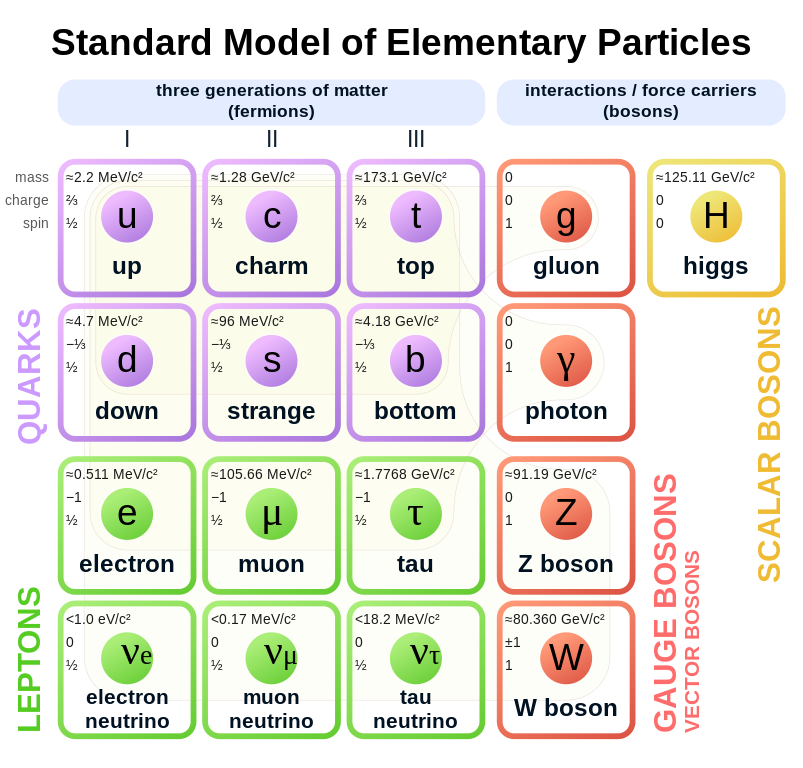
\includegraphics[width=0.8\textwidth]{Images/Theory/particlesSM.png} % TODO update to a more up to date. % TODO update the ref
    \caption[Particles in the SM]{Elementary particles of the Standard Model \cite{tableSMWiki}. Elementary fermions (quarks on top, lepton on the bottom) are listed in the three left columns and elementary bosons in the two right ones, the gauge bosons in the first column and the Higgs scalar boson in the last one. The mass, electrical charge, and spins of the particles are indicated.}
    \label{particlesSM}
\end{figure}

Particles are separated based on their intrinsic angular momentum or \textit{spin}, with half-spin particles following the Fermi-Dirac statistics called \textit{fermions}, and integer-spin particles called \textit{bosons} following the Bose-Einstein statistics. The elementary fermions are evenly split into 6 quarks and 6 leptons, with only the first generation of each being stable. The distinction between these two types stems from the different quantum numbers categorising them. Quarks carry a fractional electromagnetic charge as well as a colour charge making them sensitive to the strong interaction. On the contrary, leptons are colour-neutral and either have an electrical charge of -1$e^+$, in units of the anti-electron (positron) charge, or are neutral. The charged leptons include the electron $e^-$ - the lightest and only stable one -, the muon $\mu^-$, and the tau $\tau^-$. The neutral leptons are called neutrinos, with one neutrino $\nu_\ell$ associated per charged lepton $ell$, e.g., the electron-neutrino $\nu_e$. For the quarks, the electromagnetic charge is fractional, dividing them evenly between \textit{up}-type quarks with charge +$\frac{2}{3}$ consisting of the up $u$, charm $c$, and top $t$ flavours, and the \textit{down}-type quarks with charge -$\frac{1}{3}$ and the flavours down $d$, strange $s$, and bottom $b$. To every particle corresponds an \textit{anti}particle, with the same quantum numbers except for the electrical charge that changes sign. \\

The kinematics and dynamics of the fields representing the particles in the theory are expressed through a Lagrangian density $\mathcal{L}$, a spacetime discretisated element of the general Lagrangian. Symmetries of the Lagrangian density play an essential role as they define conserved quantities through Noether's theorem. The construction of the \gls{sm} Lagrangian id dictated by the expression of these symmetries to satisfy the experimentally observed conserved quantities, such as the electromagnetic charge. Two types of symmetries can be considered: global ones that are valid across spacetime and local ones, the so-called gauge symmetries valid for localised transformations. The \gls{sm} Lagrangian must satisfy the global Poincaré symmetry, encapsulating the symmetry required for special relativity, and a local non-Abelian $SU(3)_C \otimes SU(2)_L \otimes U(1)_Y$ gauge symmetry. Non-Abelian groups are such that their generators do not commute. The Lagrangian density of a field $\psi$ is a function of $\psi$ and its spacetime partial derivative $\partial_{\mu} \psi$, where $\mu$ indexes the time and space dimenions in the 4-vector formalism. The full \gls{sm} Lagrangian $\mathcal{L}_{\text{SM}}$ can be decomposed into 4 terms:
\begin{equation}\label{eq-SMGlobal}
    \mathcal{L}_{\text{SM}} = \mathcal{L}_{\text{EW}} + \mathcal{L}_{\text{QCD}} + \mathcal{L}_{\text{Higgs}} + \mathcal{L}_{\text{Yukawa}}.
\end{equation}
These different terms represent different effects encoded within the unified framework of the \gls{sm}. Three of the four known interactions of nature are encapuslated in the \gls{sm}: the strong, the electromagnetic, and the weak forces, with the gravitational force considered aside due to the weakness of its influence at sub-atomic scales. The mediators of the three included interactions are the gauge bosons, spin 1 particles with different properties arising from the nature of the interaction they carry. The electromagnetic and weak force have been successfully unified as a single \gls{ew} interaction, while the theory of the strong force is \gls{qcd}. One essential element in the \gls{sm} is the so-called Higgs interaction, a special force through which some gauge bosons acquire mass. This Higgs interaction is underpinned by a Higgs field, an excitation of which is called a Higgs boson $H$. Interactions between the Higgs field and quark can be introduced to assign masses to the latter through Yukawa couplings. The latter part of this thesis is dedicated to a measurement of such couplings to $b$- and $c$-quarks. The different interactions and their respective gauge bosons are further reviewed in this chapter.

\subsection{Quantum Electrodynamics}\label{subsec-QED}
\glsfirst{qed} is the theory underpinning the behaviour of free fermions and their electromagnetic interactions, for which the gauge carried are the photons. Fermions are represented by a Dirac spinor field $\psi(x)$ defined over spacetime $x$. The Dirac equation of quantum mechanics is a first order partial derivative equation modelling the free dynamics of such a spin-$\frac{1}{2}$ fermion with:
\begin{equation}\label{eq-dirac}
    (i\gamma^{\mu} \partial_{\mu} - m) \psi = 0,
\end{equation}
where $\gamma^{\mu}$ are the Dirac $\gamma$-matrices generalising the Pauli spin matrices to spacetime dimension, and the Einstein notation is adopted, summing over indices repeated as covariant and contravariant. For clarity, any contraction $\gamma^{\mu} \partial_{\mu}$ is denoted as $\cancel{\partial}$. A Lagragian density can be constructed to result in the dynamics described by Equation \ref{eq-dirac} through application of Euler-Lagrange:
\begin{equation}\label{eq-diracLag}
   \mathcal{L}_{\text{Dirac}} = \bar{\psi} (i \cancel{\partial}- m) \psi,
\end{equation}
Such a Lagrangian models the free dynamics of any spin-$\frac{1}{2}$ fermion, such as an electron $e^-$. Electrons have a $q = -1$ charge that is conserved by every known interactions. This conservations must be the result of a symmetry: the Dirac Lagrangian must be made invariant under a local gauge $U(1)$ transformation:
\begin{equation}\label{eq-GaugeU1}
    \psi \rightarrow \psi' = e^{-iq\alpha(x)} \psi ,
\end{equation}
which corresponds to a rotation in the complex spacetime by a phase $q\alpha(x)$. For the Lagrangian of Equation \ref{eq-diracLag} to satisfy this symmetry, the partial derivative $\partial_{\mu}$ must be replaced by the \textit{gauge covriant derivative $D_{\mu}$}:
\begin{equation}\label{eq-GaugeU1}
    \partial_{\mu} \rightarrow \partial_{\mu} + iqA_{\mu},
\end{equation}
where a new vector field $A\mu$ is introduced and required to transform under the $U(1)$ symmetry as $A_{\mu} \rightarrow A'_{\mu} = A_{\mu} + \partial_{\mu} \alpha(x)$. The elegance of this approach is the possibility to give this fauge field $A_{\mu}$ its own dynamic, modifying the Lagrangian of Equation \ref{eq-diracLag} into the \gls{qed} Lagrangian: \[ \mathcal{L}_{\text{QED}} = \bar{\psi} (i \cancel{\partial}- m) \psi + q \bar{\psi} \cancel{A} \psi - \frac{1}{4} F_{\mu\nu} F^{\mu\nu} \]
\begin{equation}
    \mathcal{L}_{\text{QED}} = \bar{\psi} (i \cancel{D}- m) \psi - \frac{1}{4} F_{\mu\nu} F^{\mu\nu}
\end{equation}
where $F_{\mu\nu} = \partial_{\mu} A_\nu - \partial_\nu A_{\mu} $ is the electromagnetic field tensor. The last term introduces a kinetic term for the gauge field and the interaction between the fermion $\psi$ and the gauge field $A$ is represented by the term combining them. In the present case, the charge $q$ is the conserved quantity of the gauge symmetry, which required the introduction of a new gauge field $A_\mu$ that can be interpreted as the photon field and given the dynamic of the electromagnetic interaction through $F_{\mu\nu}$. Fermionic fields can be introduced in this approach for the different known fermions, $\psi_e$, $\psi_{\mu}$, $\psi_u$, $\psi_c$, etc. Their interactions with $A_\mu$ defining each time a unique conserved electromagnetic charge $q_e$, $q_{\mu}$, $q_u$, $q_c$, etc.  This procedure is however general: the gauge invariance of a Lagrangian introduces a spin-1 gauge vector boson. The required $U(1)$ invariance forbids the presence of mass terms of the form $m^2 A^{\mu} A_{\mu}$, seemingly condemning the gauge bosons to be massless. 

\subsection{Electroweak Sector}
The weak force is described by two massive gauge vector bosons: the $W^{\pm}$ of mass $m_W \approx 80.4$ GeV\footnote{The unit system adopted throughtout this thesis is to set the speed of light in vacuum $c$ at 1, leading to masses expressed in GeV. To convert to mass units, one simply needs to divide by the standard unit $c^2$.} and the $Z^0$ of mass $m_Z \approx 91.2$ GeV. This apparent contradiction with the massless requirements of a $U(1)$ symmetry is elegantly solved by the Brout-Englert-Higgs mechanism \cite{Englert:1964et,  PhysRevLett.13.508}. This mechanism, described in the next section, is applied to a joint expression of the electromagnetic and weak forces known as \glsfirst{ew} theory in the Glashow-Weinberg-Salam (GWS) model \cite{GLASHOW1961579, PhysRevLett.19.1264, Salam:1968rm}. The fundamental symmetry group the theory is built upon is the non-Abelian $SU(2)_L \otimes U(1)_Y$, where $SU(2)_L$ is the weak isospin and $U(1)_Y$ the weak hypercharge. A local $SU(2)$ transformation acts as:
\begin{equation}\label{eq-GaugeSU2}
    \psi \rightarrow \psi' = e^{i g \alpha^a(x) T^a } \psi,
\end{equation}
where $T^a = \sigma^a / 2$ are the generators of the $SU(2)_L$ group, built from the $\sigma^a$ Pauli matrices ($a = 1, 2, 3)$. Each generator corresponds to a gauge field. The gauge field linked to $SU(2)_L$ leads to covariant derivative, simularly to Equation \ref{eq-GaugeSU2}, to ensure gauge invariance as expressed by
\begin{equation}\label{eq-GaugeSU2}
   D_{\mu}  = \partial_{\mu} + igT_a W_{\mu}^a,
\end{equation}
with three gauge fields $W_{\mu}^1$, $W_{\mu}^2$, $W_{\mu}^3$ with interaction strength $g$. The particularity of the weak interaction is that the charged current interactions described by the symmetry group $SU(2)_L$ only apply to left-handed $L$ particles states and not the right-handed $R$. Consequently, fermionic fields are decomposed into \[\psi = \psi_L + \psi_R\] with left-and right-handed particles represented by isospin doublets. The weak isospin $I_W$ charge of left-handed particles is $I_W = 1/2$, with a third component $I_W^3 = \pm  1/2$. For the right-handed part, $I_W = 0$ with $I_W^3 = 0$, decoupling it from the gauge bosons $W_{\mu}^a$. Physically, the observed weak charge current interaction corresponding to the $W^{\pm}$ bosons are the linear combinations of gauge fields:
\begin{equation}
    W_{\mu}^{\pm} = \frac{1}{\sqrt{2}} \left(W_{\mu}^{1} \mp W_{\mu}^{2} \right)
\end{equation}
These $W$ bosons only couple to left-handed particles, but an experimentally observed $Z$ boson couples to both left- and right-handed particles. This represented by the additional $U(1)_Y$ symmetry of the weak interaction in the \gls{sm}, with weak hypercharge $Y$, coupling $g'$, and an additional gauge field $B_{\mu}$. The weak hypercharge is \[Y = 2 (Q - I_W^3),\] with $Q$ the electromagnetic charge. The total covariant derivative of the electroweak sector of the \gls{sm} is therefore expressed by the GSM model as 
\begin{equation}\label{eq-GaugeEW}
    D_{\mu}  = \partial_{\mu} + ig T_a W_{\mu}^a + ig' \frac{Y}{2} B_{\mu}. % TODO should these be the g and g
\end{equation}
where $W_{\mu}^a$ and $B_{\mu}$ are respectively the $SU(2)_L$ and $U(1)_Y$ gauge bosons. The GSM model re-expresses the electromagnetic photonic field $A_\mu$ and the $Z$-boson field $Z_{\mu}$ as a linear combination of $B_{\mu}$ and $W_{\mu}^3$ depending on the \textit{weak mixing angle} $\theta_W$, a fundamental parameter of the \gls{sm} such that:
\begin{equation}\label{eq-weakmixangle}
    \cos\theta_W = \frac{g}{\sqrt{g^2 +g'^2}}.
\end{equation}
This establishes a connexion between the coupling strengths of the weak interaction and the electromagnetic interaction coupling $e$ as \[e = g \sin \theta_W = g' \sin\theta_W \cos\theta_W.\] The intrinsic strength of the weak interactions is indeed of similar ordar to that of the electromagnetic interaction but is weak in apparance due to its gauge bosons being massive. The weak force is the only known fundamental interaction to violate parity conservation. Neutrinos can only interact throught the weak force, which can itself only apply to left-handed particles. As a result, there are no right-handed neutrinos in the \gls{sm}. \\

A significant achievement of modern particle physics is the unification of interactions that are perceived as different at low-energies. The problem of the measured mass of the vector gauge bosons remains. Additionaly, the split of fermionic fields into a left- and right-handed componets lead the mass terms to violate the gauge invariance. Both issues are resolved by the mechanisn of the Brout-Englert-Higgs and Yukawa interactions, introduced in the next sections.

\subsection{The Brout-Englert-Higgs Mechanism}
The Brout-Englert-Higgs mechanism, abbreviated $BEH$ henceforth, offers a solution to introduce mass terms to the gauge fields $W_{\mu}^{\pm}$ and $Z_{\mu}$ \cite{Englert:1964et,  PhysRevLett.13.508}. It introduces a new scalar Higgs field, permeating the Universe. The field is mathematically defined as a weak isospin doublet, with a neutral component $\phi^0$ and a charged one $\phi^+$. They are jointly expressed as complex scalar field with 4 degrees of freedom:
\begin{equation}
\phi = \begin{pmatrix}
    \phi^+\\ 
    \phi^0
\end{pmatrix} = \frac{1}{2} \begin{pmatrix}
    \phi_1 + i\phi_2 \\ 
    \phi_3 + i\phi_4
\end{pmatrix}
\end{equation}
This complex scalar field is made to interact with the electroweak gauge fields as 
\begin{equation}\label{eq-HiggsLag}
    \mathcal{L_{\text{Higgs}}} = (D_{\mu}\phi)^{\dagger} (D^{\mu}\phi) - V(\phi),
 \end{equation}
where the first term described the kinetic of the $\phi$ and the second term is the Higgs potential energy:
\begin{equation}\label{eq-HiggsLag}
 V(\phi) = - \mu^2  \phi^{\dagger} \phi + \lambda (\phi^{\dagger} \phi)^2.
\end{equation}
where the expression of this potential is constrained by the need for the theory to be renormalisable. Two scalars constants govern the Higgs potential: $\mu$ and $\lambda$ describing, respectively, the quadratic and quartic interaction of the complex Higgs field $\phi$. The former manifests the interaction with the gauge bosons, while the latter introduces self-interactions. The minimum of this potential corresponds to the vacuum state. The requirement that the vacuum be stable demands $\lambda > 0$. For a positive $\mu^2 > 0$, a degenerate minimum is found at field values such that
\begin{equation}\label{eq-HiggsLag}
    \phi^{\dagger} \phi  = \frac{1}{2} (\phi_1^2 + \phi_2^2 + \phi_3^2 + \phi_4^2) = \frac{- \mu^2}{2\lambda} = \frac{v^2}{2}
\end{equation}
introducing in the last equality the so-called \textit{vacuum expectation value} $v = \sqrt{\frac{|\mu^2|}{\lambda}}$ of the field $\phi$. This infinite degeneracy of the Higgs potential minimum states underlines a special $SU(2)$ symmetry such that $\phi^{\dagger} \phi = v^2/2$. Through \textit{spontaneous symmetry breaking}, the BEH mechanism crumbles this degeneracy into one single vacuum state, typically chosen by setting the components $\phi_1 = \phi_2 = \phi_4 = 0$ and $\phi_3 = v$ so that the vacuum expactation is simply
\begin{equation}
\langle0|\phi|0 \rangle = \frac{1}{\sqrt{2}} \begin{pmatrix}
        0\\ 
        v
    \end{pmatrix}.
\end{equation}
The breaking of the symmetry enforces \[ SU(2)_L \otimes U(1)_Y \rightarrow U(1)_Q,\] with the final vacuum state correctly set as chargeless. Expanding the full field dynamic around the chosen vacuum state with a particular gauge choice to absord unphysical Goldstone fields into the vector fields called \textit{unitarity gauge} \cite{PhysRevD.7.1068}, the expansion can be simplified to 
\begin{equation}
    \phi = \frac{1}{\sqrt{2}} \begin{pmatrix}
            0\\ 
            v + h(x)
        \end{pmatrix},
\end{equation}
where $h$ is the real neutral Higgs scalar field. Introducing this expression into the Higgs Lagrangian of Equation~\ref{eq-HiggsLag} gives
\begin{equation}\label{eq-fullHiggs}
    \begin{split}
        \mathcal{L}_{\text{Higgs}} = & \,\frac{1}{2} (\partial_\mu h)(\partial^\mu h) + \frac{\mu^2}{2}(v+h)^2  - \frac{\lambda}{16}(v+h)^4 \\
        &+ \frac{1}{4} g^2 (W_{\mu}^+W^{\mu-})(v+h)^2 + \frac{g^2_W + {g'}^2}{8}(Z_{\mu}Z^{\mu})(v+h)^2 
    \end{split}
\end{equation}
where one can clearly identify mass terms for the physical gauge fields $W_{\mu}^{\pm}$ and $Z_\mu$ in the last line, but not for $A_{\mu}$ as required from observations that photons are massless. The vector gauge bosons masses are:
\begin{equation}
    m_W = \frac{v}{2} g , \, m_Z = \frac{v}{2}\sqrt{g^2 +g'^2} 
\end{equation}
or equivalenty expressing the mass of the $Z$-boson in terms of the $W$-boson mass \[m_Z = \frac{m_W}{\cos\theta_W}.\] The Higgs field is massive\footnote{This requires to isolate the terms in $h^2$ in Equation \ref{eq-fullHiggs}.} with mass \[m_H = \sqrt{2|\mu^2|}.\]
The BEH mechanism elegantly assigns mass to the gauge vector boson, with the photon remaining massless and the addition of the Higgs boson $H$ as a massive elementary particle. Furthermore, the introduction of the related Higgs field permits the expression of mass terms for the fermions in the standard model, as explained in Section~\ref{subset-yukint} on Yukawa interactions. 

\subsection{Quantum Chromodynamics}
The strong interaction is described by the theory of \textit{\glsfirst{qcd}}, underpinned by an $SU(3)_C$ symmetry with conserved quantum number called \textit{colour}. The only particles having a colour charge in the \gls{sm} are quarks and gluons $g$, the gauge mediators of the strong interactions. There are three colour charges typically labelled \textit{red}, \textit{blue}, and \textit{green}, each coming into its direct or anti-colour (e.g., anti-red). Quarks carry one such charge and gluons two. Similarly to the electroweak sector, the symmetry leads to a covariant derivative under the $SU(3)_C$ group of
\begin{equation}\label{eq-GaugeQCD}
    D_{\mu}  = \partial_{\mu} + ig_s \lambda_a G_{\mu}^a. % TODO should these be the g and g
\end{equation}
where the coupling constant $g_s$ of the strong interaction is often re-expressed as $\alpha_s = \frac{g_s}{4\pi}$, and the generator of the $SU(3)_C$ group are the set of eight $\lambda_a$ Gell-Mann matrices. The gauge field introduced here are the $G_{\mu}^a$ corresponding to the associate mediator of the strong field: the gluons $g$. Gluons carry 2 colour charges, leading to the 8 Gell-Mann matrices $\lambda^a$ and 8 gauge vector fields $G_{\mu}^a$. The generators of the $SU(3)_C$ group do not commutate: \[ [\lambda^a, \lambda^b] = i f^{abc} \lambda^c,\] where $f^{abc}$ are the $SU(3)_C$ structure constants.  Similarly to the electromagnetic strength tensor, strength tensors are built from the gluon fields as \[G_{\mu\nu}^a = \partial_{\mu} G_{\nu}^a   - \partial_{\nu} G_{\mu}^a - g_s f^{abc} G_{\mu}^b G_{\nu}^c.\]
This leads to a total \gls{qcd} Lagrangian of:
\begin{equation}\label{eq-QCDLag}
    \mathcal{L}_{\text{QCD}} = -\frac{1}{4} G_{\mu\nu}^a G^{\mu\nu}_a + \sum_{k} \bar{\psi}_k (i \cancel{D} - m_k) \psi_k,
\end{equation}
where $\psi_k$ are the six quarks fields, one per flavour, transforming as an $SU(3)_C$ triplet with one component per colour quantum number. Cubic and quartir terms in the gluon gauge fields $G_{\mu}^a$ are included, introducing self interaction of gluons. The non-commutation of the $SU(3)_C$ generators means the $SU(3)_C$ part of the \gls{sm} is non-Abelian group, and therefore a case of a Yang-Mills theory requiring this self-interacting gauge fields \cite{PhysRev.96.191}. \\

Like every coupling constant, $\alpha_s$ varies with energy. At low energies, the interaction is so strong that perturbative calculation breaks and the behaviour of \textit{colour confinement} is observed: any attempt to isolate a quark requires so much energy that a quark-antiquark pair is spontaneously produced. The strength of this interaction explains it short propagation distance despite the fact its gluonic mediatiors are massless. At higher energies $\sim 100$ GeV, asympotic freedom and perturbative calculations are possible thanks to the smallness of the coupling strength. This typically requires higher-order corrections for calculation to converge, with some terms, such as quark self-energy loops, diverging to infinity. This type of diverge is  called \textit{ultraviolet divergence}, and it is fixed by renormalising fields and parameters so that the divergence are absorbed away. This correction requires two parameters to arbitrarily define the scale of the process: the \textit{renormalisation scale} $\mu_R$ and \textit{factorisation scale} $\mu_F$ \cite{collins2004factorization}. The former is introduced to deal with ultraviolet divergences in the running of $\alpha_s$. The latter addresses the so-called \textit{infrared divergences} due to massless particles radiating further massless particles at low-energies by entering the parton distribution and fragmentation functions, introduced latter in this chapter.\\

Quarks must combine to form colour-less aggregate of matters called hadrons, with either a 2-quark system combining a quark and an antiquark into a \textit{meson}, or a 3-quark system forming a \textit{baryon} of which the proton ($uud$, $q_p = +1$) and the neutrons ($udd$, $q_n = 0$) are prime examples. The content of hadrons are called partons. The process leading to the neutralisation of the colour-charge of an asymptotically freed quark is called \textit{hadronisation}.\\

\subsection{Yukawa Interactions}\label{subset-yukint}
In the \gls{qcd} Lagrangian of Equation~\ref{eq-QCDLag}, the introduction of the mass terms for the quarks breaks the gauge invariance of the theory to $SU(2)_L \otimes U(1)_Y$ and must be therefore further modified. The masses of all fermions can however be included in the \gls{sm} by introducing so-called Yukawa interactions between the Higgs and fermionic fields. Such terms are expressed as the following Lagrangian:
\begin{equation}\label{eq-YukLag}
    \mathcal{L}_{\text{Yukawa}} = - \frac{1}{\sqrt{2}} \sum_{f} 
    y_f \bar{\psi}_f (v + h) \psi_f,
\end{equation}
where $\psi_f$ are the fermionic fields and the fundamental \textit{Yukawa coupling} parameters $y_f = \sqrt{2} \frac{m_f}{v}$ for each flavour of fermion $f$ are introduced as coupling strengths. Picking the $v$ component in the sum in parenthesis gives a clear mass term to the fermion, with the $h$ terms leading to Higgs-fermion interactions. The vacuum expectation value plays the role of a mass scale setting, with Yukawa coupling refining the specific strength for each fermionic species. For the quark sector, a futher correction is required as the weak interaction eigenstate basis is different from the mass basis in which physical particles are detected. The transformation from the mass eigenstates basis is specified by the complex unitary \textit{\gls{ckm} matrix} \cite{Tanabashi:2018oca}:
\begin{equation}
    V_{CKM} = \begin{pmatrix}
            V_{ud} & V_{us} & V_{ub}\\ 
            V_{cd} & V_{cs} & V_{cb}\\ 
            V_{td} & V_{ts} & V_{tb}\\ 
        \end{pmatrix},
\end{equation}
where the probability of a transition $p \rightarrow q$ is given by the magnitude $|V_{pq}|^2$ of the associated element. Through this quark mixing matrix, weak charged currents interaction allows for flavour-changing processes through charged currents interactions. The matrix is almost diagonal, hence transitions between quarks of the same generation are preferred (e.g., $t \rightarrow b$ preferred over $t \rightarrow d$).

\subsection{Experimental Higgs Phenomenology}
The experimental process to observe the Higgs bosons at the \gls{lhc} is to collide two proton beams head-on, as described in Chapter~\ref{chapter-ATLAS}. The accelerator is primarily designed to achieve these measurements, targeting different production and decay channels. Protons are composite particules (hadrons) and, at high energies, the main \textit{hard-scattering} interaction is beteen components of the protons called \textit{partons}. These partons are primarily the \textit{valence} quarks ($uud$ for a proton) but also contribution from \textit{sea} quarks, as well as gluons and photons present within the hadron due to quantum interactions. In a $pp$ collision, two interacting partons $ab$ from within the protons undergo the main event $ab \rightarrow X$, with the activity from the rest of the protons assigned to the so-called \textit{\gls{ue}}. The cross-section for the global process $pp \rightarrow X$ is expressed using the factorisation theorem \cite{collins2004factorization}: 
\begin{equation}
\sigma_{pp\rightarrow X} \sum_{a,b} \int_0^1 dx_a \int_0^1 dx_b f_a(x_a, \mu_F) f_b(x_b, \mu_F) \int d\sigma_{ab\rightarrow X}\left(x_aP_a, x_bP_b, \mu_R, \mu_F \right),
\end{equation}
where $f_i(x_i, \mu_F)$ is the \textit{\gls{pdf}} giving the probability for the parton $i$ to undergo a hard scattering with momentum $p_i = x_i P_i$, where $x_i$ is the fraction of the proton momentum $P_i$, $\mu_F$ is the previously introduced factorisation scale, as the \gls{pdf} depend on the energy scale of the underlying process. The interaction is effectively split into two steps: picking up the interacting partons and their fraction of momentum, then considering the main $ab \rightarrow X$ event.\\

As introduces in the previous section, the Higgs couples to particles proportionally to their measured mass, which influences its production and decay modes. The leading order production modes of the Higgs boson are schematised in Figure \ref{fig:prodH}. At the \gls{lhc} with a centre of mass energy $\sqrt{s} = 13$ TeV and a Higgs boson mass $m_H = 125$ GeV, the main processes presented are by decreasing cross-sections: 
\begin{itemize}[leftmargin=*] % TODO check values % TODO check for qqH
    \item \textit{Gluon-gluon fusion $ggF$}: two gluons fuse into a quark loop with a radiated Higgs boson: $pp \rightarrow H$. The quarks in the loop must couple to the Higgs, hence top $t$-quarks are preferred, followed by bottom $b$-quarks. The cross-section for this process is $\sigma_{ggF} = 48.6 \pm 2.4$ pb \cite{LHCHiggsCrossSectionWorkingGroup:2016ypw}. This process is favoured thanks the large contributions of gluons to the protonic \gls{pdf}s.
    \item \textit{Vector boson fusion $VBF$}: two off-shell vector bosons $V$ ($W$ or $Z$) radiated from partonic quarks fuse to form a Higgs $pp \rightarrow qqH$, with cross-section $\sigma_{VBF} = 3.77 \pm 0.09$ pb \cite{LHCHiggsCrossSectionWorkingGroup:2016ypw}. The quarks leave a characteristic twin forward jets in the event.
    \item \textit{Associated production with a vector boson $VH$}: the Higgs boson is produced in association with a vector boson $V$ ($W$ or $Z$): $pp \rightarrow VH$. This process is studied in greater detail in Chapter~\ref{}, dedicated to an analysis of Higgs decaying to $b$- or $c$-quarks from this production mode. It has a cross-section of $\sigma_{VH} = 2.24 \pm 0.14$ pb \cite{LHCHiggsCrossSectionWorkingGroup:2016ypw}. Leptonic decays of the associated vector boson give clean event signatures.
    \item \textit{Associated production with a quark pair $q\bar{q}H$}: an ``open quark loop'' is produced from a pair of partonic gluons, with a Higgs radiated $pp \rightarrow q\bar{q}H$. The dominating contributions come from the $t\bar{t}H$ associated production with cross-section $\sigma_{VH} = 0.51 \pm 0.04$ pb, followed by the $b\bar{b}H$ \cite{LHCHiggsCrossSectionWorkingGroup:2016ypw}.
\end{itemize}

\begin{figure}[h!]
    \center
    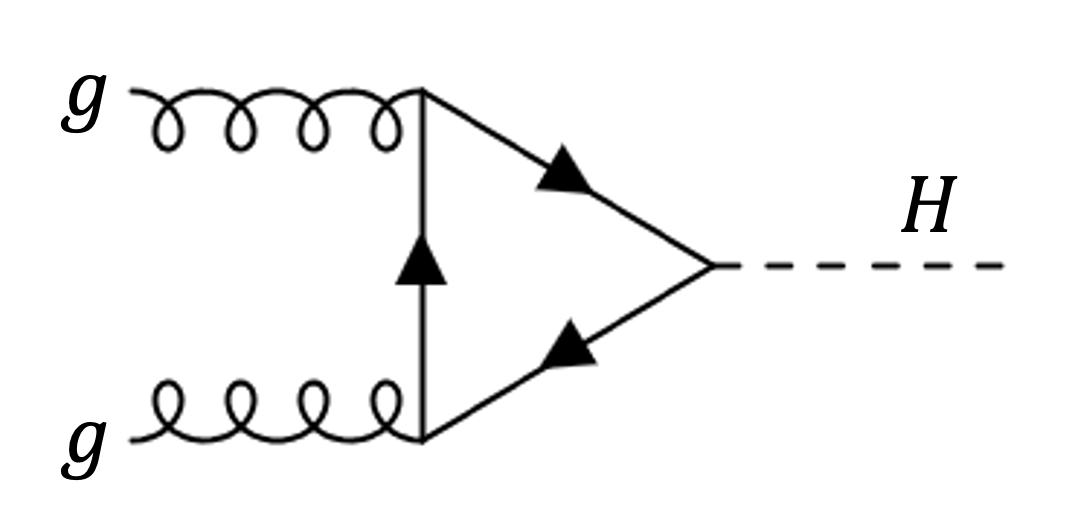
\includegraphics[width=0.24\textwidth]{Images/Theory/ggH.png}
    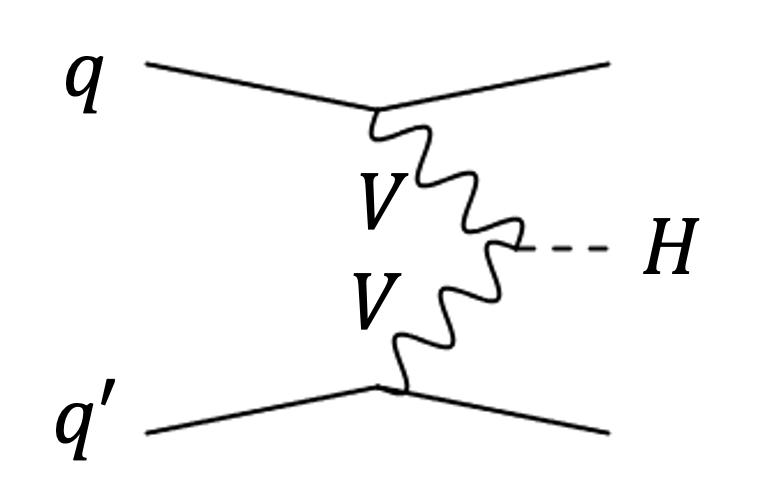
\includegraphics[width=0.24\textwidth]{Images/Theory/vvH.png}
    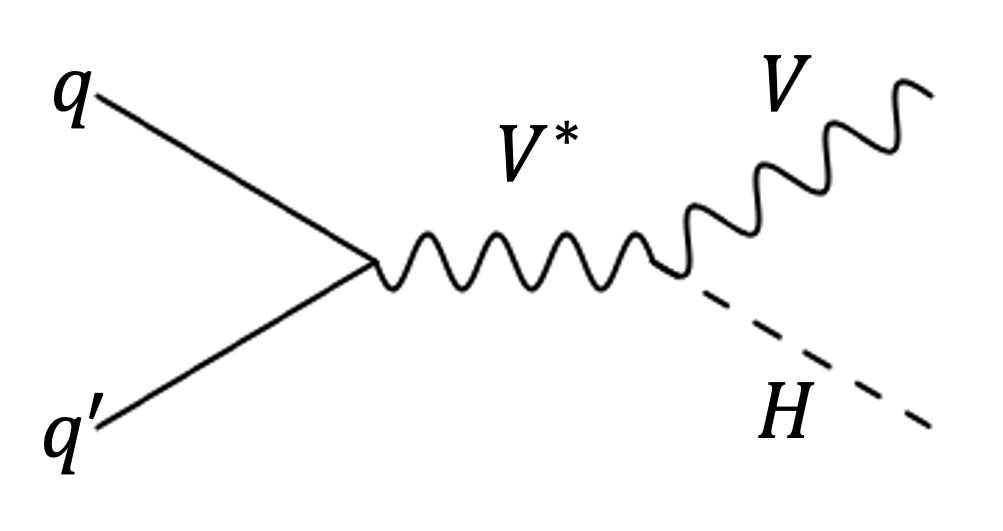
\includegraphics[width=0.24\textwidth]{Images/Theory/vh.png}
    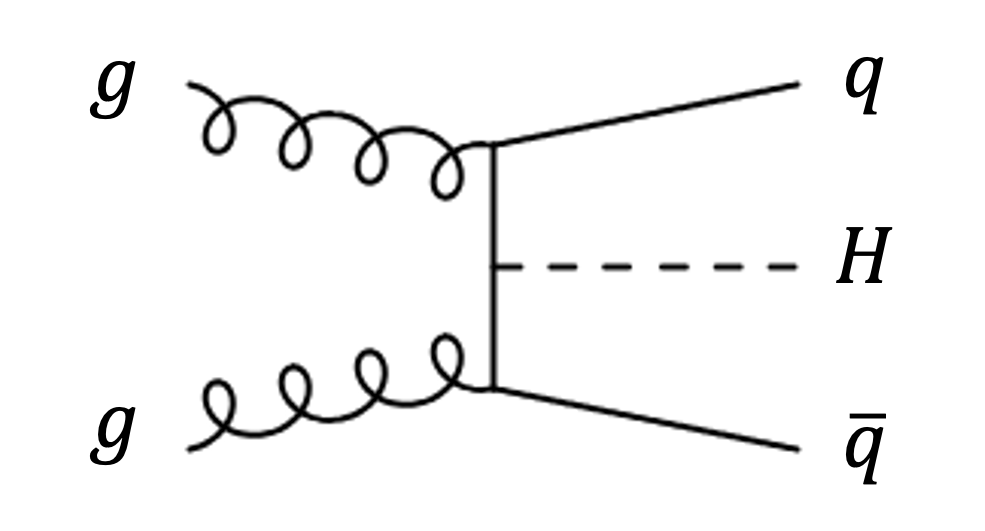
\includegraphics[width=0.24\textwidth]{Images/Theory/qqH.png}
    \caption{The leading order Feynman diagrams for Higgs production at the LHC, from left to right: gluon-gluon fusion ($ggF$), vector boson $V$ fusion ($VBF$), associated production with a vector boson ($VH$), and associated production with a $q\bar{q}$ pair ($q\bar{q}H$).}
    \label{fig:prodH}
\end{figure}

The dependency of the Higgs boson production from proton-proton collisions at $\sqrt{s} = 13$ TeV are represented in the left of Figure~\ref{fig:prodH} as a function of the Higgs boson mass $m_H$. The total width of the \gls{sm} Higgs boson is $\Gamma_H = 4$ MeV, implying a short lifetime of $\tau_H ~ 10^{-22}$ $s$ and restricting measurement to its decay products. The decay branching ratios are displayed in the right of the figure, with decays to heavier particles favoured due to the proportionality of the Higgs coupling strength to the mass. Decays to the massless gluons $g$ and photons $\gamma$ are possible thanks to intermediate quark loops, similarly to $ggF$. Relative decay rates are quantified by their branching ratio $BR$ as
\begin{equation}
    BR(H \rightarrow X) = \frac{\Gamma(H\rightarrow X)}{\Gamma_H}
\end{equation},
where the total Higgs width $\Gamma_H$ is the sum of all partial decay width $\Gamma(H\rightarrow X)$, for all possible $X$. The right of Figure~\ref{fig:prodH} displays the \gls{sm} Higgs branching ratio at $\sqrt{s} = 13$ TeV. The most likely Higgs decay mode is to a pair $b\bar{b}$ ($BR \approx 58$ \%), followed by the decay to a $WW$ pair ($BR \approx 21$ \%), and the $c\bar{c}$ decay branching ratio is 2.9\%. All the decay branching ratios are displayed in the right of the figure, with decays to heavier particles favoured due to the proportionality of the Higgs coupling strength to the mass. \\

\begin{figure}[h!]
    \center
    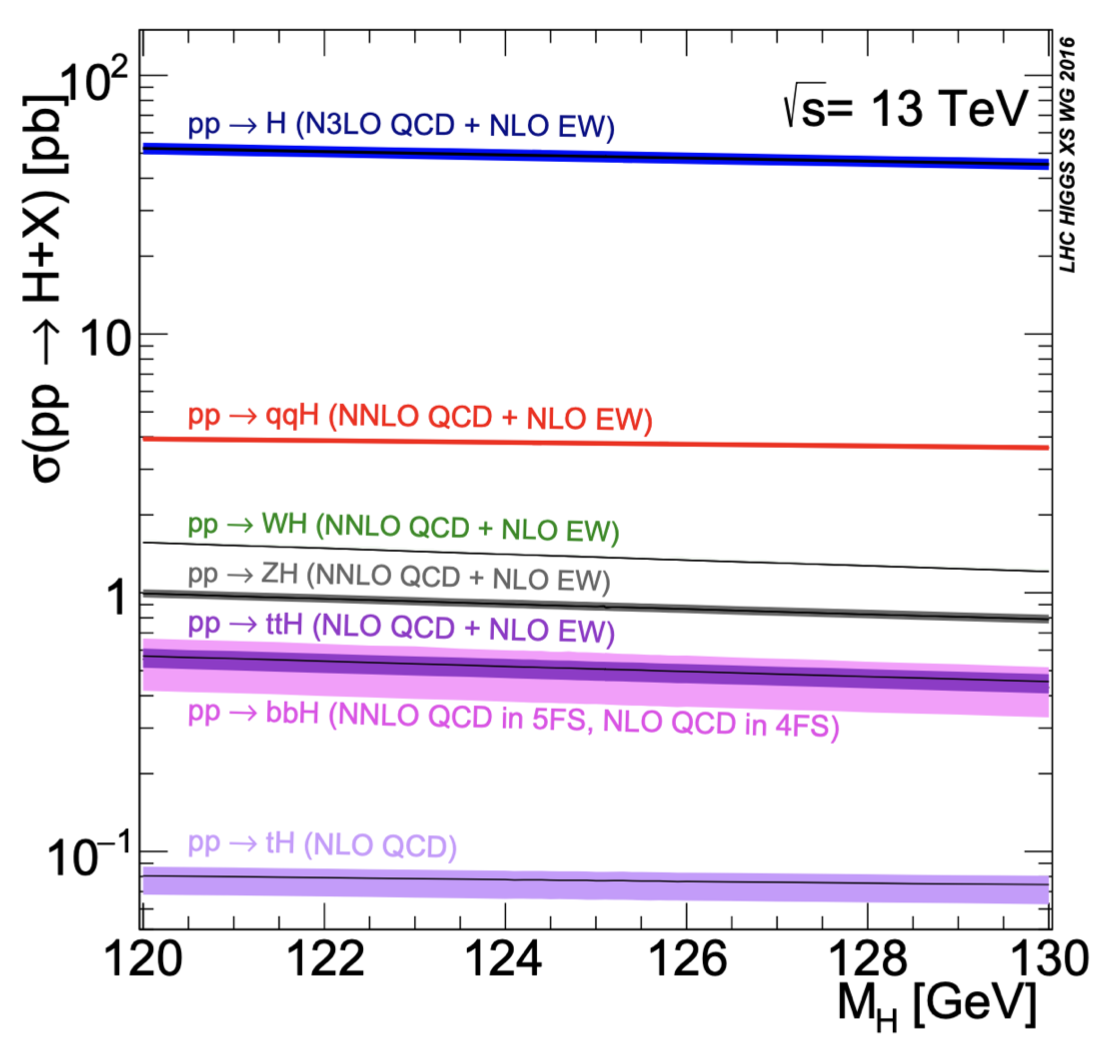
\includegraphics[width=0.48\textwidth]{Images/Theory/prodHiggs.png}
    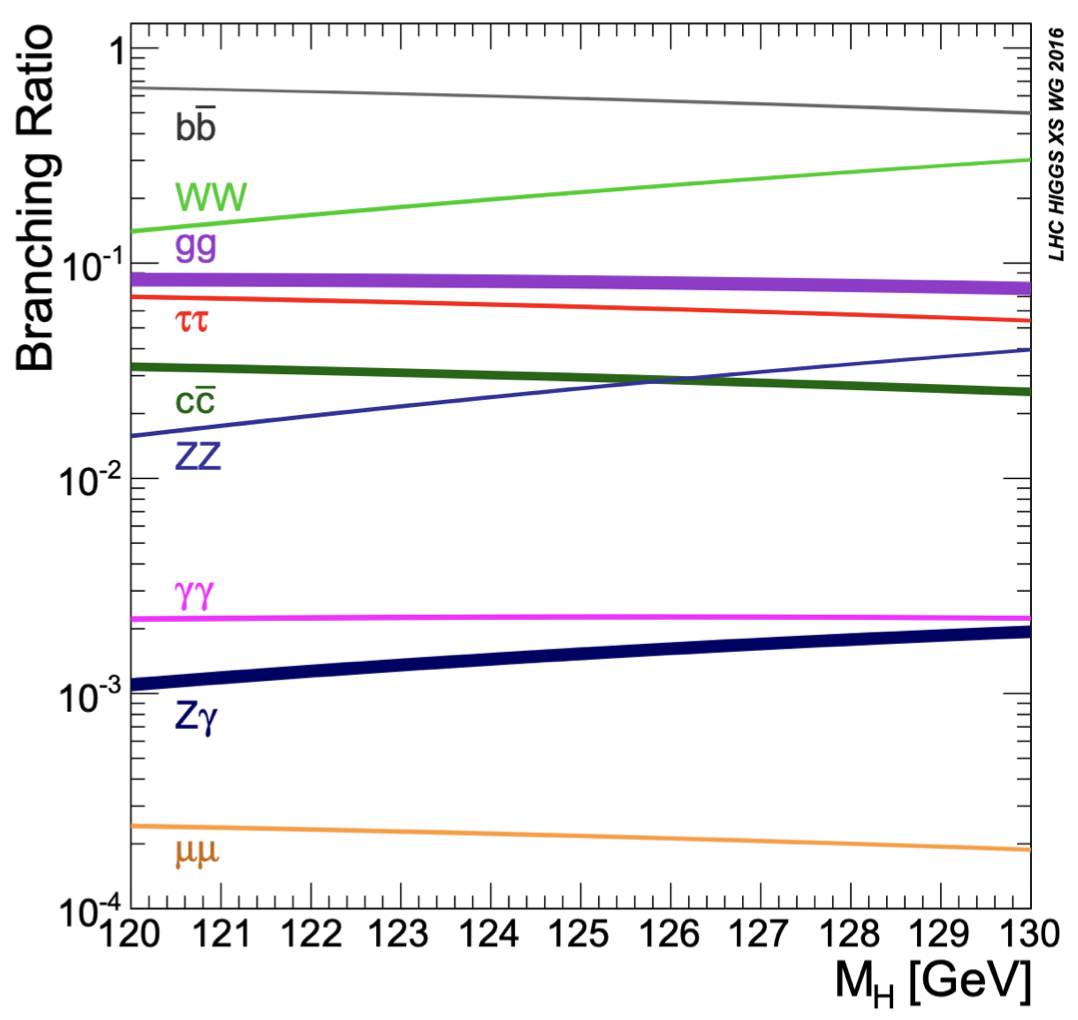
\includegraphics[width=0.48\textwidth]{Images/Theory/decayHiggs.png}
    \caption{The Standard Model production cross-sections from proton-proton collisions (left) and decay branching ratio (right) of the Higgs boson as a function of $m_H$, at $\sqrt{s} = 13$ TeV, from \cite{LHCHiggsCrossSectionWorkingGroup:2016ypw}.}
    \label{fig:prodH}
\end{figure}
\begin{figure}[h!]
    \hspace{-0.48cm}
    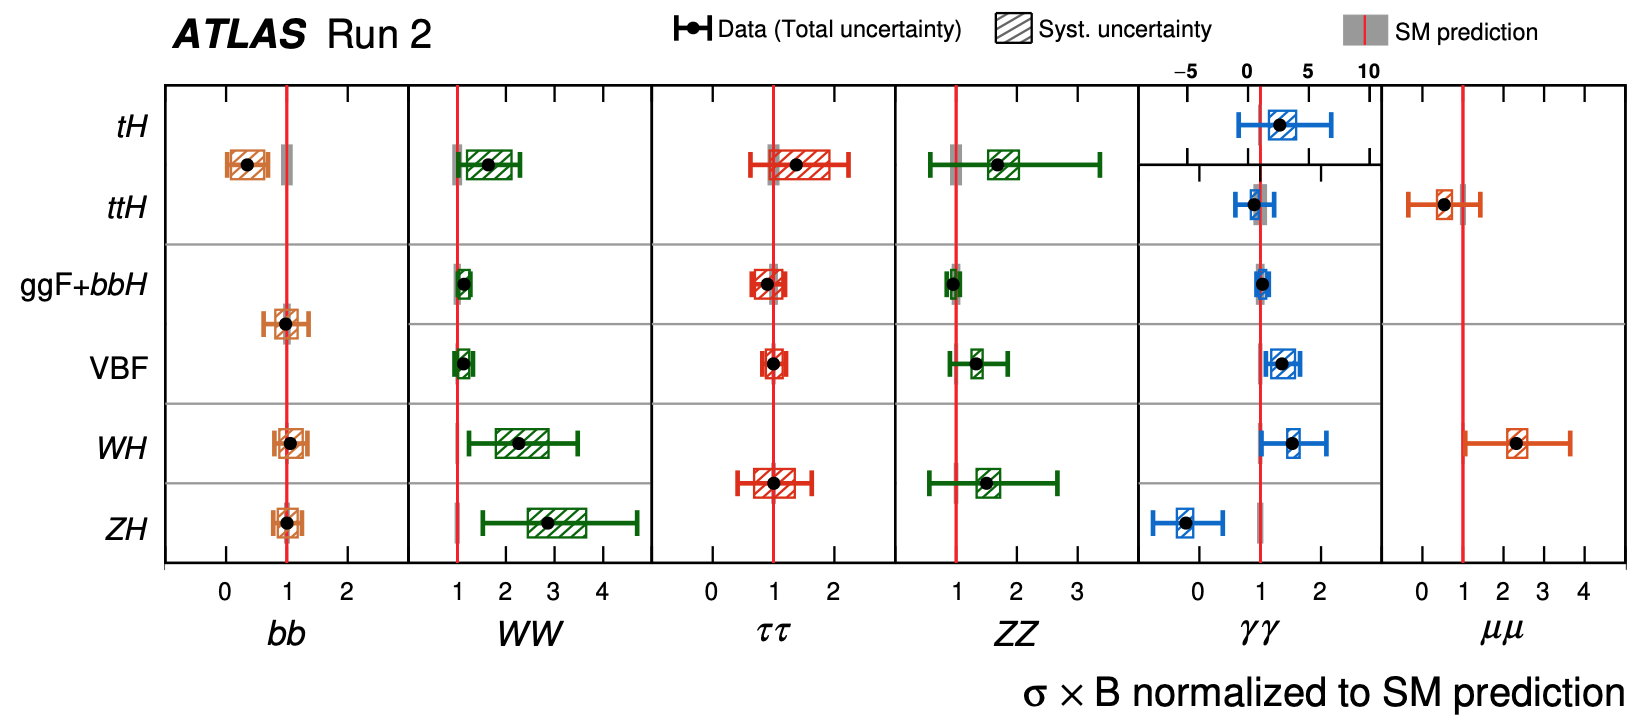
\includegraphics[width=\textwidth]{Images/Theory/allMesRun2.png}
    \caption{Ratio of observed to the SM predicted event rate for different combinations of Higgs boson production and decay mode, from \cite{ATLAS:2022vkf}. The horizontal bars denote the 68\% confidence interval, with grey bands showing the theory uncertainties on the SM cross-section $\times$ branching ratio predictions.}
    \label{fig:measprodH}
\end{figure}

The $W^+W^-$ and $ZZ$ decays can only be achieved by a virtual off-shell Higgs bosons. The fermionic decays are hard to observe due to the larger multi-jet background in a hadron collider. The vector bosons and di-photons leptonic decays benefit from advantageous experimental conditions, being easier to identify thanks to the presence of leptons and suffering from less background contamination. For these reasons, the ATLAS and CMS experiment both observed a particle of mass $m_H = 125$ GeV with the same properties as the Higgs boson in 2012 by combining the $H \rightarrow \gamma\gamma$, $H \rightarrow ZZ \rightarrow \ell^+\ell^-\ell'^+\ell'^-$, and $H \rightarrow W^+W^- \rightarrow \ell^+\ell^-\nu \bar{\nu}$ channels \cite{ATLAS:2012yve, CMS:2012qbp}. This opened the way to many additional Higgs measurements, with some of the most sensitive ones summarised in Figure \ref{fig:measprodH}. Decay modes to third generations particles ($t, b, \tau$) have been observed, with the sensitivity rising for the second generation ($\mu$). In all analyses, the Higgs boson is measured to be in remarkably consistent with the predictions from the \gls{sm} \cite{ATLAS:2022vkf}. 


\newpage
\chapter{\color{oxfordblue} The LHC \& ATLAS Experiment}\label{chapter-ATLAS}
\ChapFrame

\textit{
Modern particle physics explores the frontier of the technological reach of science. A remarkably complex infrastructure was necessary to probe physics at the required scale to discover the Higgs boson. The \gls{cern} hosts the largest and most powerful particle accelerator ever built: the \glsreset{lhc}\gls{lhc}. It has held this title since its construction concluded in 2008 \cite{LyndonEvans_2008}, and ranks among the most intricate machines ever created. Protons are accelerated to 99.9999991\% of the speed of light in a giant 27 km-long ring-shaped beamline, located 100 m below the surface of the French-Swiss border in the suburbs of Geneva. Superconducting magnets cooled with liquid helium to 1.9 $K$ steer this energetic beam thanks to powerful magnetic fields of 8.33 Tesla. The beams, composed of bunches of particles, collide at four precise interaction points where large detectors are built and operated by dedicated collaborations: ATLAS \cite{TheATLASCollaboration_2008}, CMS \cite{TheCMSCollaboration_2008}, ALICE \cite{TheALICECollaboration_2008}, and LHC$b$ \cite{TheLHCbCollaboration_2008}. The first two are multipurpose experiments with overlapping physics programs, while ALICE and LHC$b$ respectively study heavy-ion and heavy-flavour physics. This chapter describes the experimental setup of the \gls{lhc} and the ATLAS experiment, focusing on proton-proton collisions and introducing relevant elements for the work presented in this thesis.} 

\section{The Large Hadron Collider}\label{sec-LHC}
The last machine in the complex multi-stage accelerator system of CERN depicted in Figure \ref{fig-CernAccSys}, the \glsreset{lhc}\gls{lhc} is capable of frontally colliding proton or heavy ion beams packed into bunches. The beams collide at four interaction points, where dedicated experiments such as ATLAS measure the resulting physics signatures in large detectors designed for their specific physics programmes. The life of a proton beam starts in a bottle of ionised hydrogen ($H^-$) gas, the contents of which are passed through a linear accelerator called \textsc{linac} 4\footnote{\textsc{linac} 2 before 2020.} to reach an energy of 160 MeV \cite{Vretenar:2020quc}. After stripping the ionised hydrogen atoms of their two electrons to leave bare protons, the next acceleration stage happens in the Proton Synchrotron Booster (\textsc{booster}), bringing the beam's energy to 2 GeV \cite{Reich:1969fw}. The protons are then handed to increasingly larger synchrotrons: the Proton Synchrotron (\textsc{ps}) to reach an energy of 26 GeV \cite{CERNPS}, followed by the Super Proton Synchrotron (\textsc{sps}) to reach an energy of 450 GeV \cite{Synchrotron:1997188}. The beam is finally injected into the \gls{lhc} in two different beamlines circulating the proton in opposite directions \cite{Evans:2008zzb}. Superconducting dipole magnets generating an 8.33 T field steer the highly energetic beams, while complex geometries of magnets, such as quadrupoles and sextupoles, refine the bunch shape through focusing effects. Powerful radiofrequency cavities accelerate the protons to their final energy of 6.5 TeV each, giving a total $pp$ collision centre-of-mass energy of $\sqrt{s} = 13$ TeV in Run 2. 

\begin{figure}[!h]
  \centering
  \makebox[\textwidth][c]{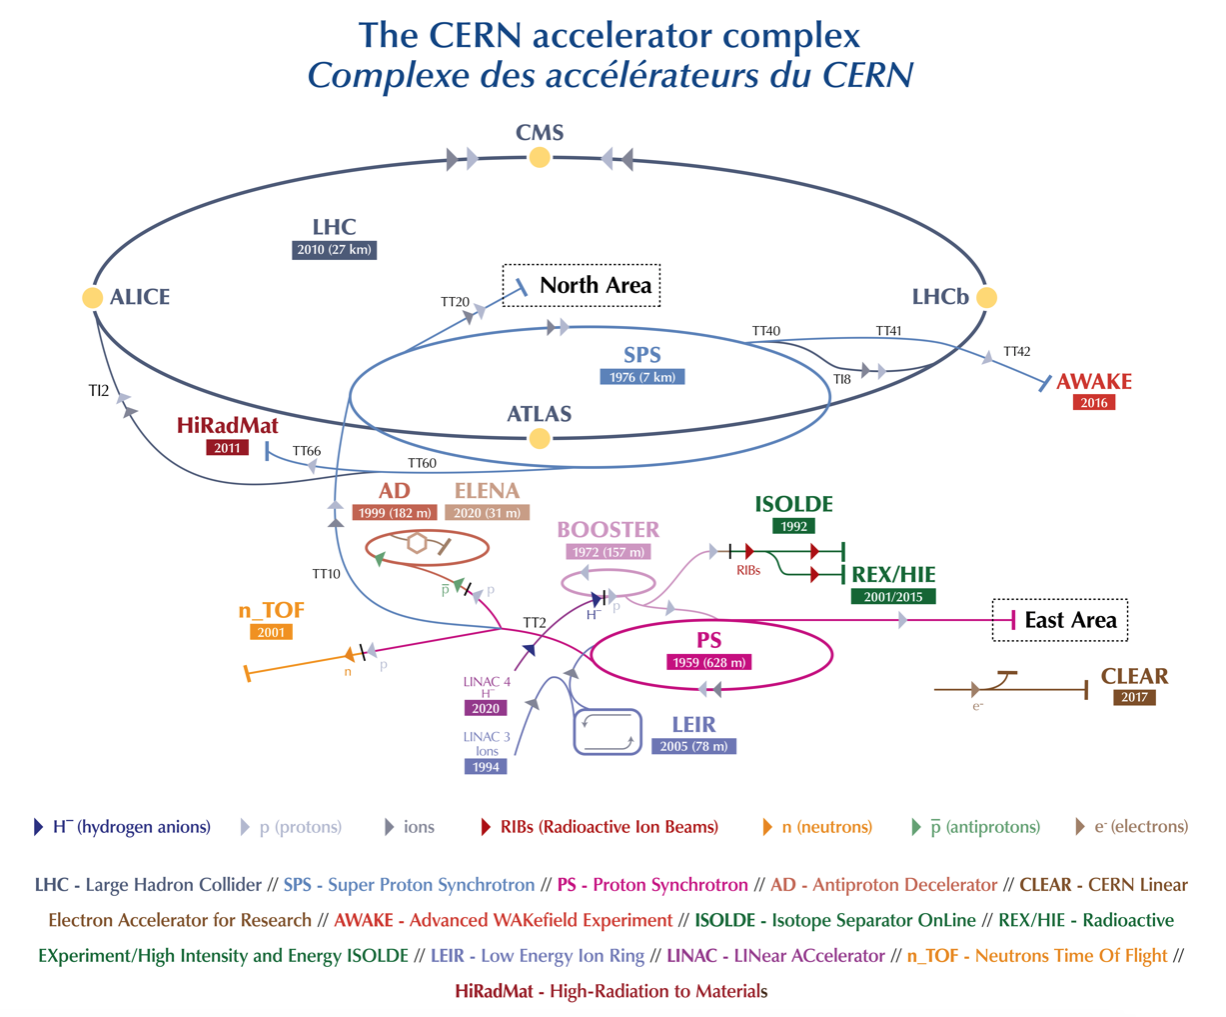
\includegraphics[width=1.05\textwidth]{Images/ATLAS/cernAcc}}
  \caption{The complete accelerator complex of CERN for Run 3 \cite{CERNAcc}.}
  \label{fig-CernAccSys}
\end{figure}

The operation of the \gls{lhc} is split into dedicated \textit{runs} of data-taking separated by \textit{shutdowns} to maintain or upgrade the infrastructure. Key metrics about these runs from the point of view of the ATLAS experiment are displayed in Table~\ref{tbl:LHCATLASperf}. Run 2 operated at a larger centre-of-mass energy ($\sqrt{s}$) and higher average instantaneous luminosity ($\mathcal{L}$) than Run 1.

%\vspace{-1cm}
\begin{table}[!htbp]
  \begin{center}
      \renewcommand{\arraystretch}{1.2}
    %\resizebox{0.99\textwidth}{!}{
      \begin{tabular}{cc|cccc} \hline \hline 
        & Year & $\sqrt{s}$ [TeV] & $\langle \mu \rangle$ &  Luminosity $\mathcal{L}$ [cm$^{-2}$s$^{-1}$] & $\int\mathcal{L}$ [fb$^{-1}$] \\ \hline
        Run 1 & 2010 - 2012 & 7-8    & 18 & 0.8 $\times$ $10^{34}$    & $26.4$ \\
        Run 2 & 2015 - 2018 & 13     & 34 & 1-2 $\times$ $10^{34}$  & $140.1$ \\
        Run 3 & 2022 - 2025 & 13.6     & 50 & 2 $\times$ $10^{33}$    & $65$ \\

        \hline\hline
      \end{tabular}
    %}
    \caption{Metrics on the accelerator performance of the LHC in the different runs of data taking. The reported values correspond to those recorded by the ATLAS experiment \cite{ATLAS:run1Lumi, ATLAS:2022hro, ATL-DAPR-PUB-2023-001}. Numbers for the ongoing Run 3 are preliminary, with the integrated luminosity listed considering events recorded until July 2023. The number of interactions per bunch crossing averaged over each run is displayed as $\langle \mu \rangle$.}
    \label{tbl:LHCATLASperf}
  \end{center}
\end{table}

The average instantaneous luminosity $\mathcal{L}$ measures the rate of data collection as
\begin{equation}
  \frac{dN}{dt} = \mathcal{L} \times \sigma,
\end{equation}
relating the event rate of a particular process to its cross section $\sigma$. The instantaneous luminosity is a machine parameter: it depends on the design and the operation of the accelerator. It is calculated from
\begin{equation}
  \mathcal{L} = \frac{N_1N_2N_bf}{4\pi\sigma_x\sigma_y}
\end{equation}
where $N_1$ and $N_2$ are the numbers of protons in each bunch, $N_b$ the number of bunches, $f$ is the collider revolution frequency, and $\sigma_x$ and $\sigma_y$ are the geometrical extensions of the beam density distribution in the $x$- and $y$-directions. The integrated luminosity $\int \mathcal{L}\, dt$ measures the number of events collected over a certain period, often expressed in units of inverse \textit{barn} b$^{-1}$, where 1 b $= 10^{-28}$ m$^{2}$. For Run 2, the total luminosity recorded by ATLAS corresponds to 140.1 $\pm$ 1.2 fb$^{-1}$, with a small uncertainty of 0.83\% \cite{ATLAS:2022hro} thanks to a complex measurement involving luminosity-dedicated detectors such as LUCID-2 \cite{Avoni_2018}. Figure \ref{fig-atlasLumiPileup} shows the cumulative distribution of the integrated luminosity during Run 2, along with another important machine parameter: the average number of interactions per bunch crossing $\langle \mu\rangle$.

\begin{figure}[!h]
  \centering
  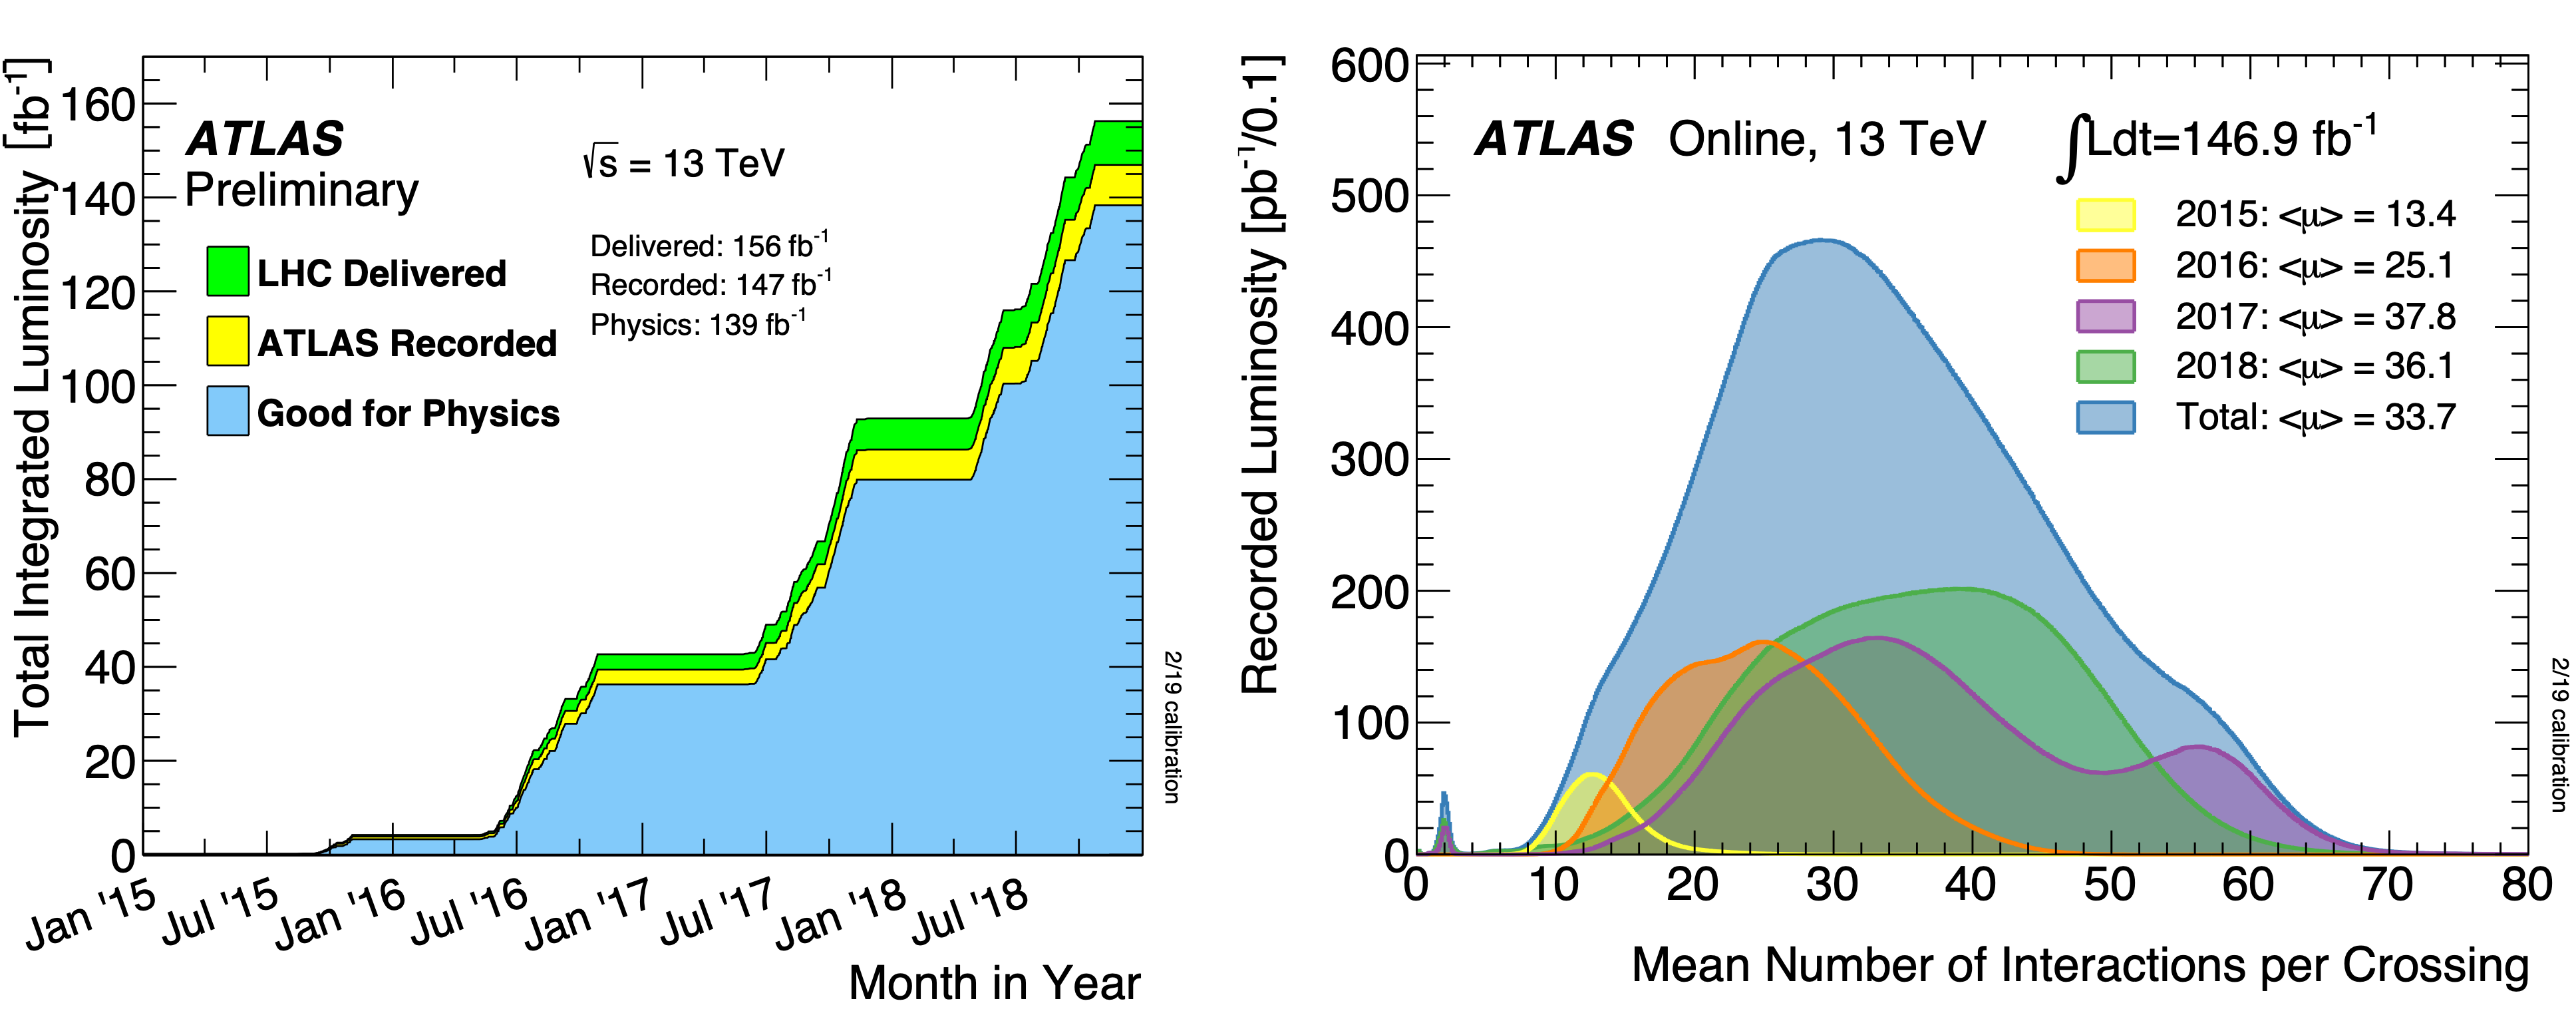
\includegraphics[width=\textwidth]{Images/ATLAS/recoATLAS.png}
  \caption{The cumulative integrated luminosity delivered, recorded, and useful for physics (left), and the average luminosity-weighted pile-up distribution (right) during Run 2 at ATLAS \cite{PubAtlasLumi}. The luminosities listed correspond to an early calculation that was refined in Ref. \cite{ATLAS:2022hro}.}
  \label{fig-atlasLumiPileup}
\end{figure}

The main event during the collisions of two protons is the inelastic hard scattering, where most of the energy transfer occurs. Other protons in the bunches can have softer interactions, leading to background activity referred to as \textit{\gls{pu}}. Two types of pile-up are distinguished: \textit{in-time \gls{pu}} when the soft interaction is from protons in the same bunch as those involved in the hard scattering, and \textit{out-of-time \gls{pu}} if the protons are from bunch-crossings just before or after the collision of interest. The \gls{lhc} separates bunches by a 25 ns delay, corresponding to a machine frequency of 40 MHz. To control the luminosity, the angle of attack of the beams is tweaked so that their geometrical overlap, measured by $\sigma_x$ and $\sigma_y$, at the point of impact is tunable. Having more head-on collisions leads to a larger overlap and higher luminosity but comes at the price of more \gls{pu}. 

\section{The ATLAS Detector}\label{sec-ATLASDet}
The ATLAS Collaboration maintains and operates the eponymous cylindrically shaped multi-layered detector, lying 100 m underground, with a length of 45 m and a diameter of 26 m \cite{TheATLASCollaboration_2008}, as presented in Figure~\ref{fig-AtlasDec}. The experiment is designed to probe a broad range of physical phenomena. Aiming to be as hermetic as possible, the detector wraps around the interaction point, with the barrel forming the central part of the cylinder and the endcaps closing the geometry at its extremities. Essential requirements in the technical design had to be met to manage the extreme event rate, requiring a fast response from radiation-hard sensors with state-of-the-art readout electronics in combination with good spatial and temporal resolution to disentangle the effect of pile-up.

\begin{figure}[!h]
\centering
\hspace{-1.25cm}
\makebox[\textwidth][c]{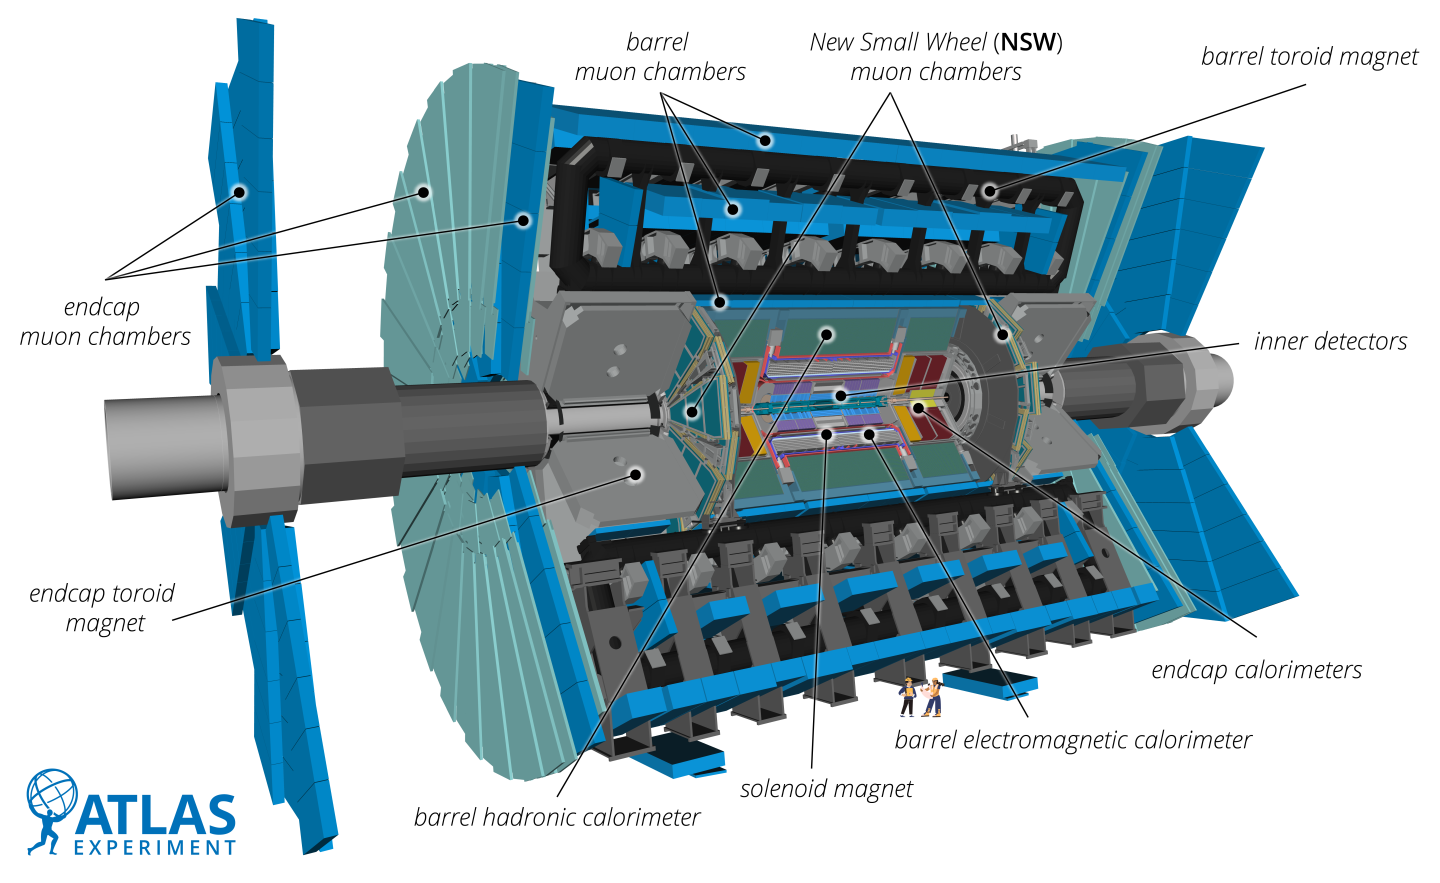
\includegraphics[width=1.08\textwidth]{Images/ATLAS/atlasDet.png}}
\caption{Cut-away view of the ATLAS detector \cite{ATLASschematics}.}
\label{fig-AtlasDec}
\end{figure}

\newpage
The coordinate system adopted in ATLAS is described in Figure \ref{fig-AtlasCoord}: the $x$-axis points to the centre of the \gls{lhc} ring, the $y$-axis points upwards, and the $z$-axis is in the longitudinal direction along the beamline, anti-clockwise when viewed from above. The azimuthal angle $\phi$ is defined in the transverse plane $x-y$, and the polar angle $\theta$ is measured upwards from the beam axis. The transverse momentum \pt\ of a particle is obtained from its momentum vector $\boldsymbol{p} = (p_x, p_y, p_z)$, of magnitude $p$, as \pt\ $= p \sin\theta = \sqrt{p_x^2 + p_y^2}$. This projection plays a crucial role, as the longitudinal component $p_z$ is not fully resolvable due to the openings for the beamline and the interacting partons carrying only a fraction of the original proton momenta. Therefore, only the transverse momentum can be reliably measured. Since the partons are mostly longitudinally boosted, the transverse momenta in an event are approximately balanced. The rapidity $y$ of a particle is expressed as 
\begin{equation}
  y = \frac{1}{2} \ln \left(\frac{E + p_z}{E - p_z}\right)
\end{equation}
with $E$ and $p_z$ the energy and longitudinal momentum of the particle. In the ultrarelativistic limit, when $p >> m$, the rest mass is negligible, and $E \approx p$. In this case, the rapidity $y$ is well approximated by the experimentally reconstructable pseudorapidity $\eta$:
\begin{equation}
  \eta = -\ln \left(\tan \frac{\theta}{2}\right).
\end{equation}
At high energies, $\Delta \eta$ becomes approximately invariant under Lorentz boosts along the $z$-axis. The pseudorapidity is often combined with the azimuthal angular aperture $\Delta \phi$ to define the angular separation $\Delta R$ between two objects as
\begin{equation}\label{eq-def-deltaR}
  \Delta R = \sqrt{\Delta \phi^2 + \Delta \eta^2} =  \sqrt{\Delta (\phi_2 - \phi_1)^2 + \Delta (\eta_2 - \eta_1)^2}.
\end{equation}

\begin{figure}[!h]
  \centering
  %\hspace{+0.5cm}
  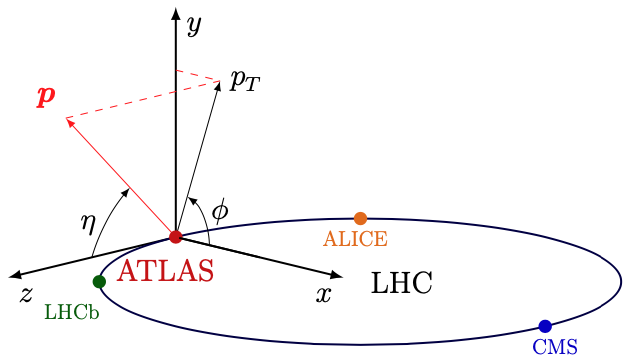
\includegraphics[width=0.6\textwidth]{Images/ATLAS/atlasCoor.png}
  \caption{The ATLAS coordinate system \cite{Strong:2020mge}.}
  \label{fig-AtlasCoord}
\end{figure}

As depicted in Figure~\ref{fig-AtlasDec}, ATLAS is composed of many subdetectors measuring information in the range $|\eta|<  2.5$, with some specialised subdetectors such as the calorimeters extending further. An essential feature of the detector is its magnetic fields. In ATLAS, they are provided by four superconducting magnets: the \textit{Central Solenoid}, which generates a 2 T axial magnetic field used by the central trackers, and a tangential magnetic field of about 1 T at the muon detectors, achieved by the \textit{Barrel Toroid} and the two \textit{Endcap Toroids}. A $q$-charged particle of momentum $p$ is deflected by a magnetic field $B$ due to the Lorentz force, leading to a relation between the radius of curvature $R$ of the trajectory and the momentum $p$ such that 
\begin{equation}
  p_{\perp} = 0.3 \, qBR \, [\text{GeV}/c],
\end{equation}
where $p_{\perp}$ is the magnitude of the momentum perpendicular to the magnetic field $\boldsymbol{B}$, and $q$ is expressed in the unit of proton charge. Therefore, the component of the momentum transverse to the magnitude $B$ can be inferred by measuring the curvature. Higher magnetic fields induce larger curvature, simplifying the measurement of $R$ and improving the resolution of $p_{\perp}$. \\ 

The rest of this chapter reviews the different subdetectors of ATLAS and introduces some common reconstruction methods that are relevant to the work presented in this thesis. 

\subsection{The Inner Detector Tracker}
The detector placed closest to the beam crossing point is the \textit{\gls{id}} \cite{CERN-LHCC-97-016}. This tracker, covering the range $|\eta| < 2.5$ in a radius of 3 cm to 1 m, is designed to record localised energy deposits called \textit{hits} in silicon semiconductors or straw tubes from the passage of charged particles. Subsequently, the trajectories or \textit{tracks} of these particles can be reconstructed by combining these signatures. The powerful 2 T magnetic field of the Central Solenoid enables this detector to measure both the charge and the momentum of charged particles. The \gls{id} combines three subsystems, represented in Figure \ref{fig-AtlasDecID}. 

\begin{figure}[!h]
  \centering
  \hspace{-1.25cm}
  \makebox[\textwidth][c]{\includegraphics[width=1.1\textwidth]{Images/ATLAS/ATLASinDecComb.png}}
  \caption{The Inner Detector of ATLAS \cite{ATLASschematics}.}
  \label{fig-AtlasDecID}
\end{figure}

First, the high-granularity \textit{Pixel Detector} covers the innermost region with three barrel and three endcap layers, for a total of 80 million sensitive semiconductor pixels \cite{CERN-LHCC-97-016, Potamianos:2015lar}. During Run 2, an additional \textit{\gls{ibl}} with 12 million pixels was added at a radius of 33 mm \cite{Capeans:1291633}. This detector gives robust and precise tracking performance and plays a major role in flavour tagging, as described in Chapter~\ref{chap-ftag}. The pixel dimensions range from 50 $\times$ 400 $\mu$m$^2$ in the Pixel Detector to 50 $\times$ 250 $\mu$m$^2$ in the \gls{ibl}, where the smaller dimension is used for the $R\phi$ measurement. The geometrical position resolution delivered is of 10 $\mu$m (67 $\mu$m) in the transverse $R\phi$ plane ($z$-direction) \cite{Pernegger_2015, ATL-INDET-PUB-2016-001}. \\

The \textit{\gls{sct}} is the next detector, constructed by arranging pairs of silicon microstrips layers into modules assembled into 4 concentric barrel layers and 9 disks in each endcap \cite{AHMAD200798, CERN-LHCC-2017-005}. The resolution is of 17 $\mu$m in $R\phi$ and 580 $\mu$m in $z$ \cite{ATLASSCT}. \\

The final system is the \textit{\gls{trt}}, a gas-based straw-tube tracker aiding track reconstruction by delivering numerous hits \cite{TheATLASTRTcollaboration_2008}. Approximately 300,000 drift tubes of a 4 mm diameter filled with a mixture of argon and xenon are arranged along the beamline in the barrel and radially in the endcaps. Each tube is fitted with a conducting wire at its centre and the surface is electrically charged, so that the passage of a charged particle ionises the gas leading to a measurable signal. Polyethylene is placed between the tubes to encourage the emission of transition radiations from relativistic particles proportionally to their Lorentz boost $\gamma \sim E / m$. The \gls{trt} is used for both tracking and electron and pion identification, by reconstructing the mass of the charged particles from the amount of $\gamma$-radiation. For tracking, the position resolution is 130 $\mu$m in the $R\phi$ plane for the barrel and the $z\phi$ plane for the endcaps \cite{Vogel:1537991}. \\

Altogether, the track inverse transverse momentum resolution of the ATLAS \gls{id} is
\begin{equation}
  \sigma(1 / p_T) = 0.36 \oplus \frac{13}{p_T \sin\theta} \text{TeV}^{-1}
\end{equation}
where $\oplus$ denotes a sum in quadrature \cite{TheATLASCollaboration_2008}. This corresponds to a relative error of about 0.01\% for a track with \pt\ $\sim$ 500 MeV, and 4\% at a \pt\ $\sim$ 100 GeV.

\subsection{Electronic and Hadronic Calorimeters}
Covering the $|\eta| < 4.9$ region, calorimeters collect the energy of all interacting particles, neutral and charged. The system is composed of an \textit{\gls{ecal}} and a \textit{\gls{hcal}}, both covering the $|\eta| < 3.2$ central region, and a forward calorimeter for the $3.2 < |\eta| < 4.9$ region \cite{TheATLASCollaboration_2008}, as displayed in Figure~\ref{fig-AtlasDecCalo}.\\

The \gls{ecal} is designed to collect the energy of electrons and photons and contributes to the measurement of the energy of jets. The active material is \gls{lar}, with absorbing plates of lead used as passive material to encourage \textit{bremsstrahlung}, $e \rightarrow e\gamma$, and pair production from photons, $\gamma \rightarrow e^+e^-$. The \gls{ecal} has a depth of at least 22 $X_0$, where the unit of \textit{radiation length} $X_0$ tracks the distance for an electron to retain only 1/$e$ of its original energy. The energy resolution is parametrised into three terms representing the sampling term, the electric noise, and a constant contribution for miscalibrations, summed in quadrature as \cite{Cavallari_2011}
\begin{equation}
  \frac{\sigma_E^{\text{ECAL}}(E)}{E} = \frac{10\%}{\sqrt{E}} \oplus \frac{0.17 [\text{GeV}]}{E} \oplus 0.7\%,
\end{equation}
giving an energy resolution between $\sim$0.5\% for 10 GeV electrons, and $\sim$ 0.6\% for 60 GeV photons.\\

\begin{figure}[!h]
  \centering
  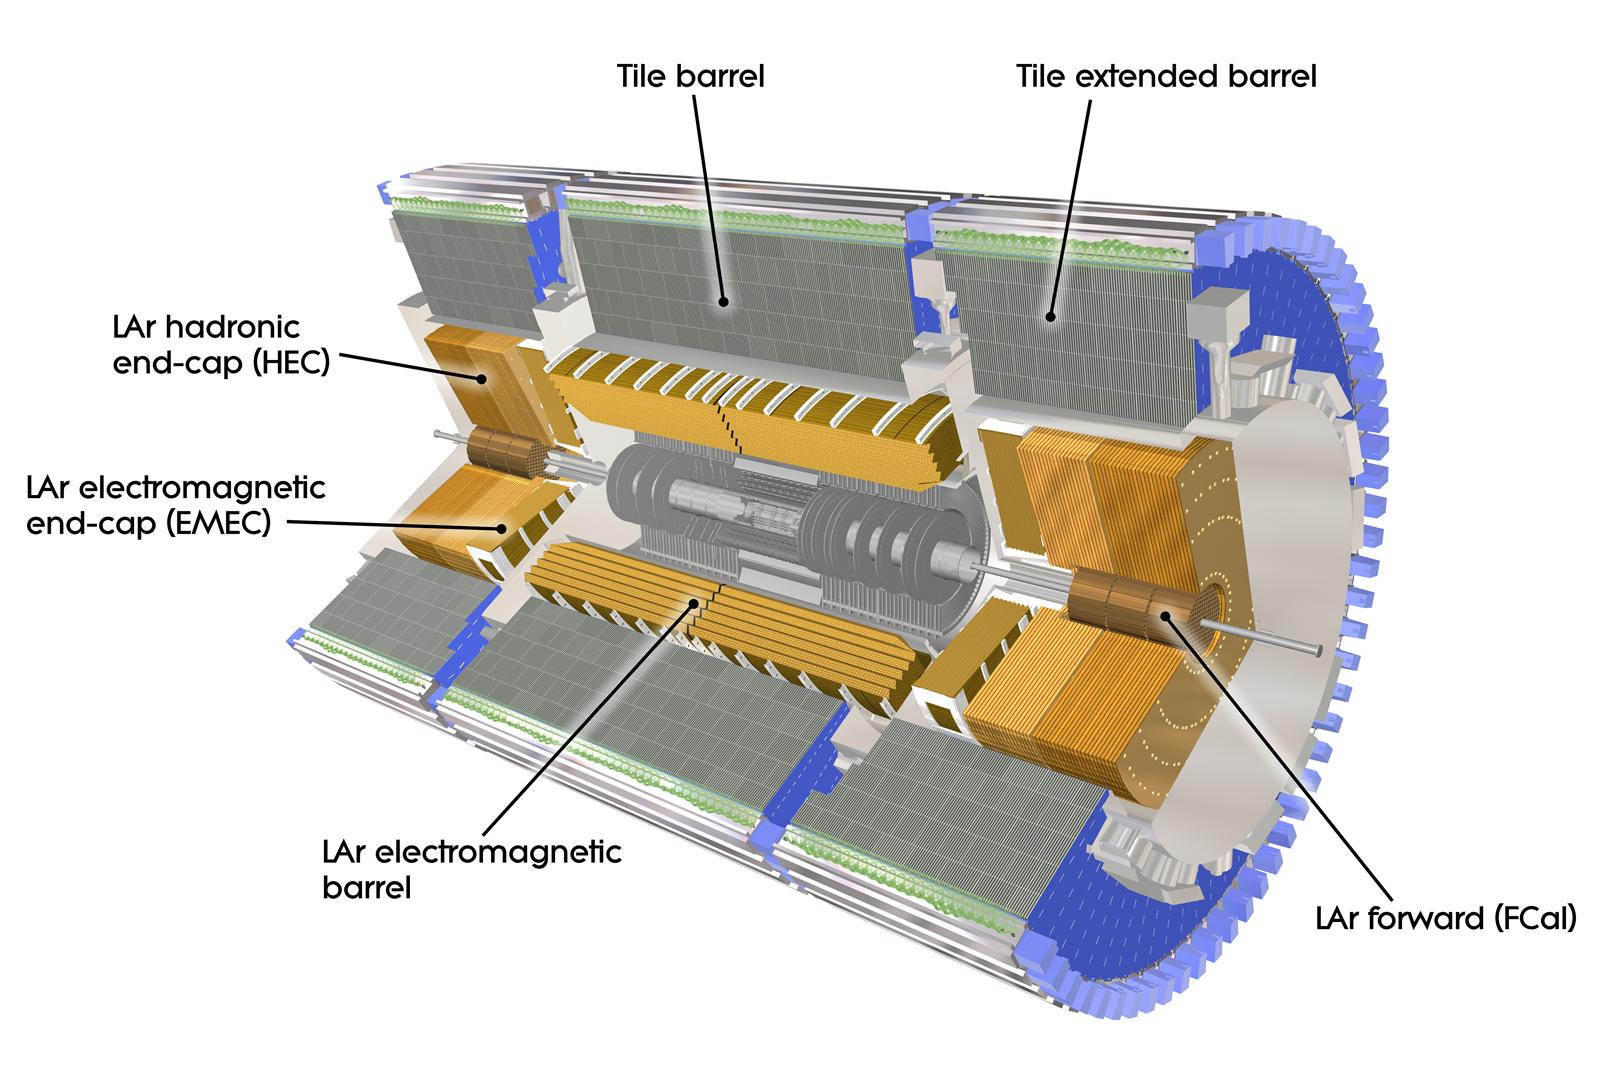
\includegraphics[width=\textwidth]{Images/ATLAS/ATLASCalo.jpg}
  \caption{The calorimeter systems of ATLAS \cite{ATLASschematics}.}
  \label{fig-AtlasDecCalo}
\end{figure}

The \gls{hcal} is designed to capture the energy of hadronic showers, with \gls{lar} as active material for the endcap and forward calorimeters and scintillating plastic tiles for the barrel. As passive material, the endcaps use copper plates, the forward calorimeters use copper and tungsten, and the tile calorimeter in the barrel uses steel. The depth of the hadronic calorimeter is approximately $10 \lambda$, where $\lambda$ is the nuclear interaction length tracking the average distance before a hadron interacts with a nucleus. The calorimeters collect the majority of the energy of hadrons, with an \gls{hcal} resolution expressed as \cite{Cavallari_2011}
\begin{equation}
  \frac{\sigma_E^{\text{HCAL}}(E)}{E} = \frac{52.9\%}{\sqrt{E}} \oplus 5.7\%.
\end{equation}
This translates into a resolution of $\sim$17\% ($\sim$6\%) at energies of $\sim$10 GeV ($\sim$100 GeV).

\subsection{Muon Detection Systems}
Muons require dedicated detection systems to be efficiently and precisely reconstructed. While they leave good tracks in the \gls{id}, muons do not leave much energy in the calorimeters due to their high mass-suppressing bremsstrahlung radiations. For this reason, the outermost subdetectors of ATLAS are specially designed to be sensitive to muons. The \textit{\gls{ms}}, shown in Figure~\ref{fig-AtlasDecMuon}, is a dedicated muon tracking system that also provides an effective triggering hardware, as described later in this chapter. The muon tracker is composed of drift tubes split between the barrel region for $|\eta| < 1.2$ and the endcaps $1.2 < |\eta| < 2.7$, with cathode strip chambers in the inner layers of the endcaps. The trigger system relies on resistive plate chambers in the barrel and thin gap chambers in the endcaps. To improve momentum and charge measurements from the reconstructed tracks, powerful superconducting toroidal magnets are used to deflect muons in the \gls{ms}. The resolution on \pt\ is measured to be of $\sim 2.3$\% (2.9\%) for muons from $Z$ decays in the central (forward) region \cite{atlasMuonPTReco}.

\begin{figure}[!h]
  \centering
  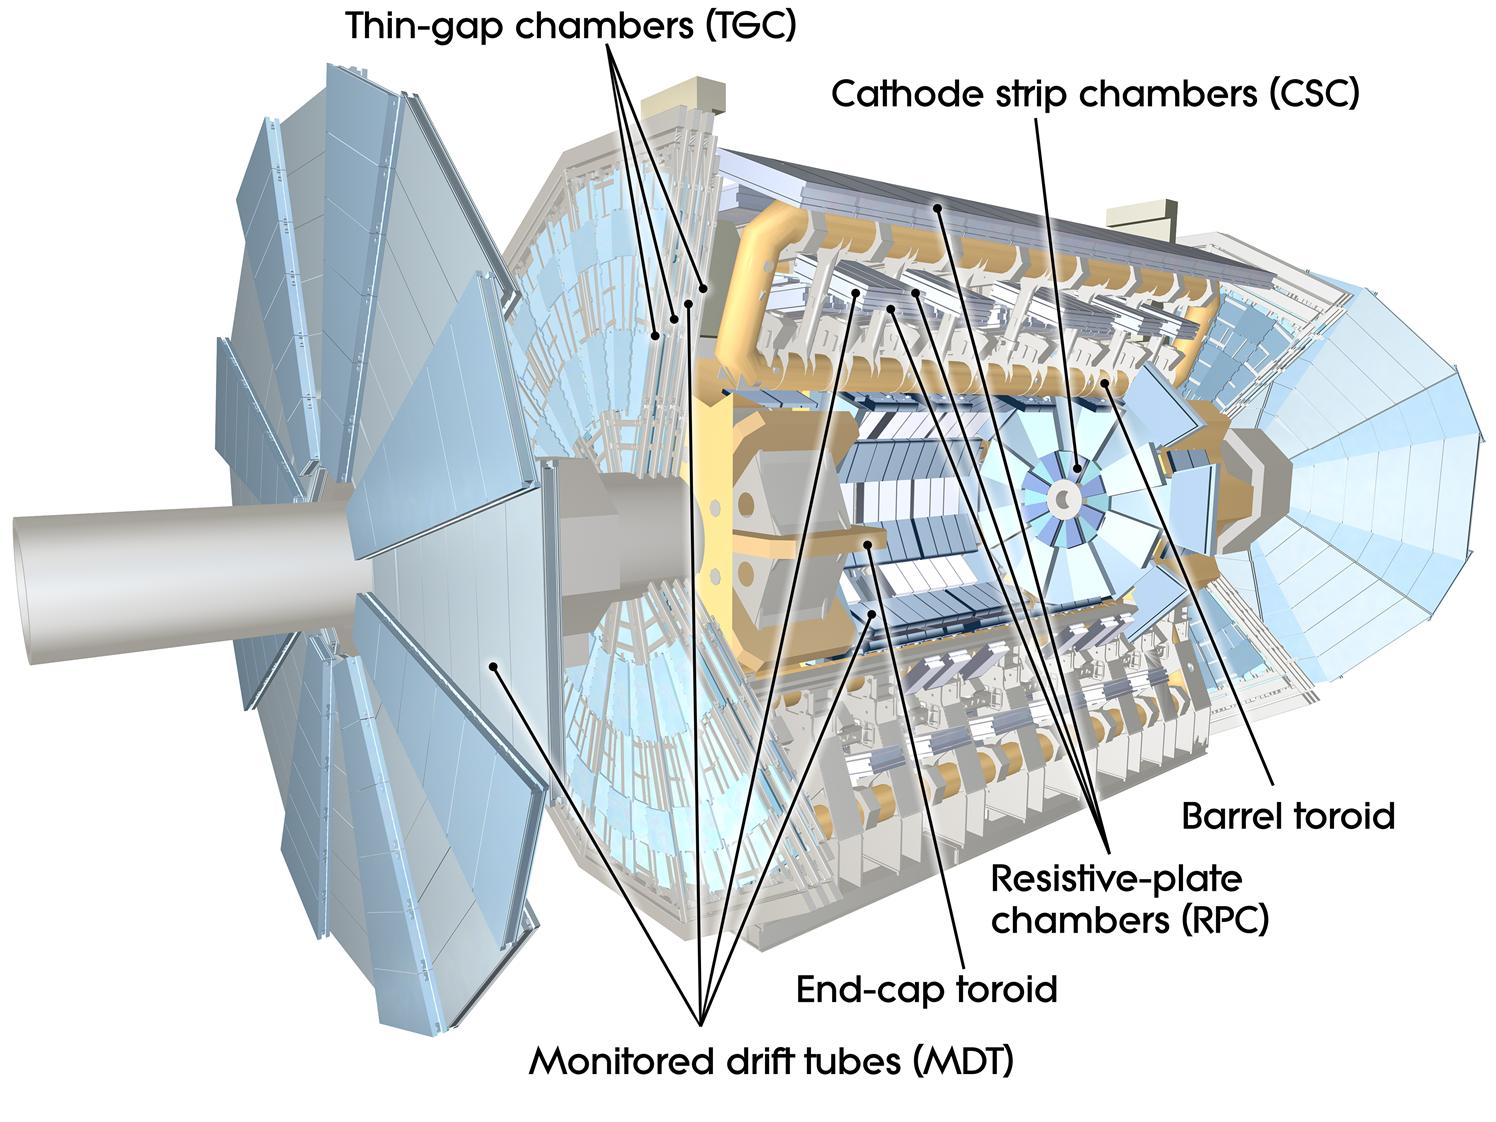
\includegraphics[width=0.9\textwidth]{Images/ATLAS/ATLASMuon.jpg}
  \caption{The muon detectors of ATLAS \cite{ATLASschematics}.}
  \label{fig-AtlasDecMuon}
\end{figure}

\section{Operation and Reconstruction with the ATLAS Detector}\label{chap-atlas-reco}
For physics-quality data taking, the different subdetectors of ATLAS must be performing according to specifications. In operation, the event rate produced by the \gls{lhc} in the heart of the ATLAS detector is 40 MHz, due to the 25 ns bunch-crossing. This unfortunately leads to a data generation rate that is too high for the computing resources available, requiring the Collaboration to design specific approaches to reduce the rate to a manageable level \cite{Nedden_2017}. This is the task of the trigger system, which is described in this section. Events that pass the trigger thresholds are stored and must be further analysed to reconstruct the physics processes from the low-level measurements performed by the different subdetectors: this is the task of reconstruction, the last subject described in this chapter for object types relevant to the presented work. This latter step is performed thanks to the extensive ATLAS software \cite{ATL-SOFT-PUB-2021-001, ATL-SOFT-PUB-2020-001}, exploiting the specific signatures of the different detected particles as schematised in Figure~\ref{fig-ATLASdetect}.

\begin{figure}[!h]
  \centering
  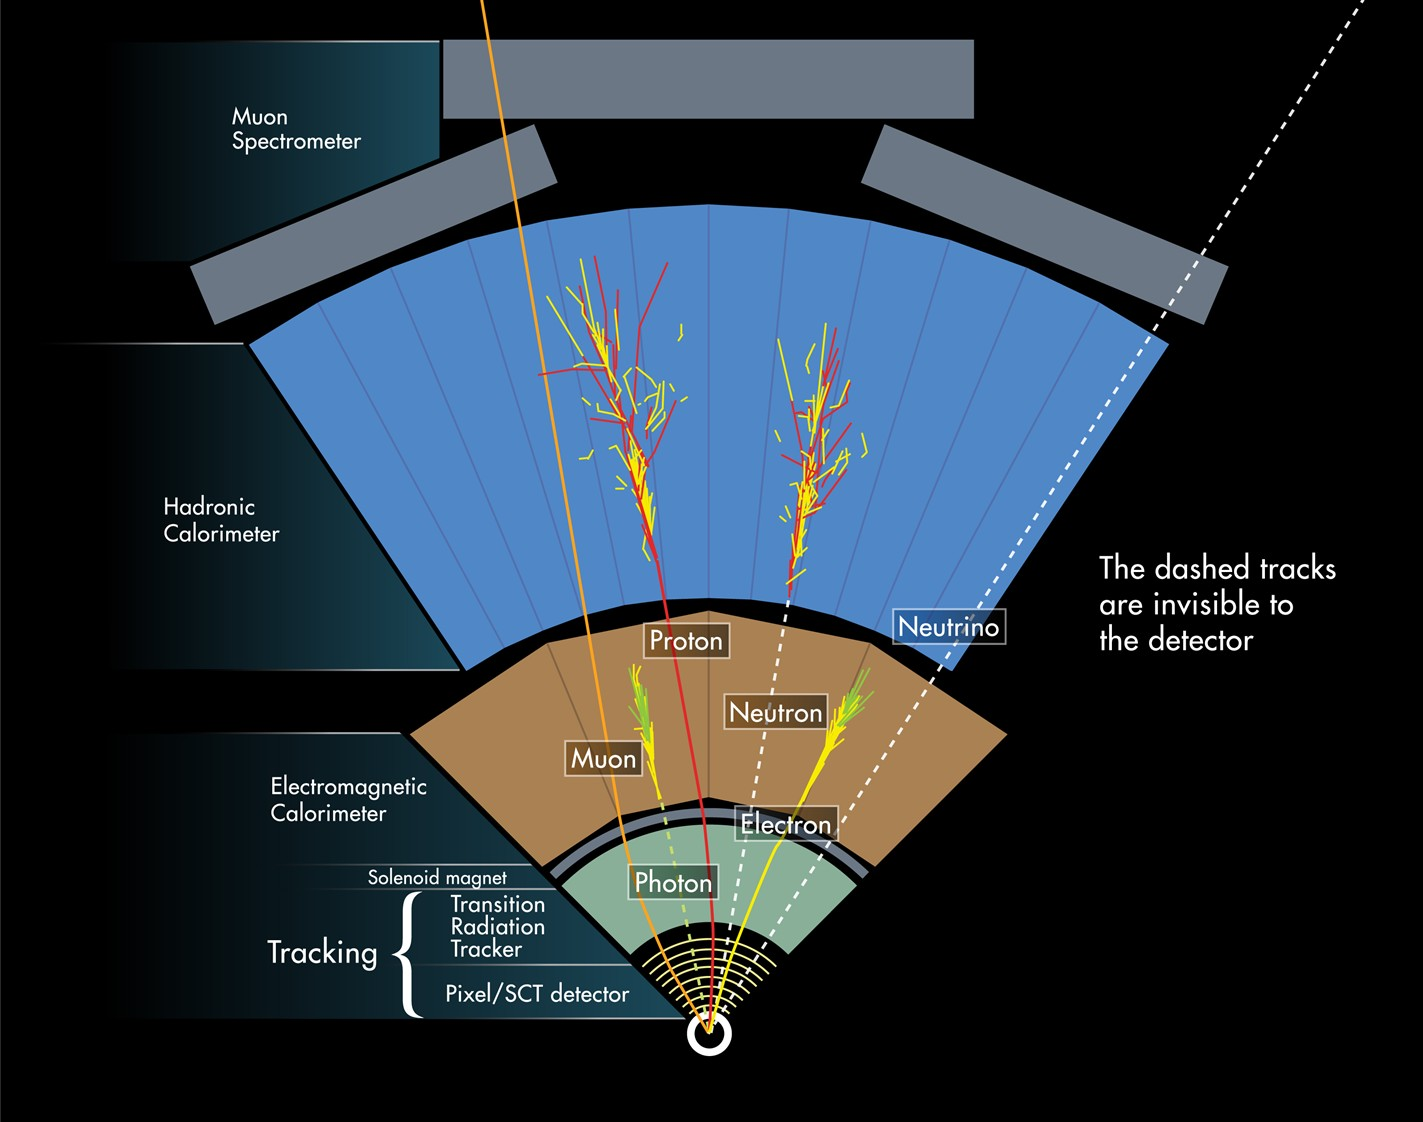
\includegraphics[width=\textwidth]{Images/ATLAS/ATLASdetection.jpg} %0.8
  \caption{Schematics of different particles signatures in the ATLAS detector \cite{Pequenao:1505342}.}
  \label{fig-ATLASdetect}
\end{figure}

\subsection{Trigger System}\label{sub-sec-trigger}
The ATLAS trigger system relies on a hierarchical approach to progressively reduce the data rate and select events deemed interesting for physics. Firstly, the Level-1 (L1) trigger is built on fast electronic hardware accessing coarse information to reduce the rate to 100 kHz in $\sim$ 2.5 $\mu$s. This is followed by the High-Level Trigger (HLT) that runs on a farm of 40,000 \glspl{cpu} to implement a finer software-based selection, bringing the rate down to 1.2 kHz or 1.2 GB/s, suitable for data storage \cite{TriggerATLAScollaboration_2020}. In this process, increasingly complex information is accessed by dedicated readout and measurement systems. Some commonly used triggers are based on signatures of electrons, muons, missing transverse energy, and $b$-jets. Different trigger menus are designed by the Collaboration, with dedicated data-taking periods for each setup. Analyses can then select data collected with the optimal trigger stream for the specific signatures sought.

\subsection{Low-Level Signatures: Tracks, Vertices, and Clusters}\label{sec-atlas-lw}
Low-level signatures are used in higher-level reconstruction processes to identify physics objects, such as electrons and jets. Three types are described here: the trajectory of charged particles called \textit{tracks}, the construction of vertices, and the formation of calorimeter clusters. \\

Tracks are the reconstructed trajectories of charged particles through the detector from the collected localised energy deposits called \textit{hits}. A \textit{hole} is a missing hit in a sensitive detector element when one is expected based on the reconstructed track trajectory. With denser pile-up activity, the number of hits in a single event becomes significant, making track reconstruction a computationally challenging problem \cite{ATL-PHYS-PUB-2015-006, ATLAS-tracks-algo,}. The trajectories are curved due to the previously described superconducting magnets. From a set of hits, tracks are fitted inside-out \cite{ATLAS-tracks-algo}: clusters of three hits in the Pixel or \gls{sct} detectors are first identified as \textit{seeds}, with additional hits associated by a combinatorial Kalman Filter \cite{10.1115/1.3662552} based on compatibility criteria with the initial track. Hits can initially be shared by several tracks, with the ambiguity resolved later when the reconstructed tracks are ranked by quality and $\chi^2$ fits are performed to quantify the best possible association while favouring high \pt\ tracks. The process is then extended to the \gls{trt} from the outside-in, and followed by additional quality criteria such as requiring tracks to have a \pt\ > 500 MeV in $|\eta| < 2.5$, a minimum of 7 hits in the Pixel and \gls{sct}, at most one hole, and at most two shared hits. Tracks are parameterised by the longitudinal (along $z$) and transverse (in the $x-y$ plane) \glspl{ip}, respectively $z_0$ and $d_0$, measuring the distance from the \gls{pv} to the point of closest approach of the track (the perigee). \\

If a reconstructed charged particle is produced in the hard scattering event, its trajectory leads back to a location called the \textit{\glsreset{pv}\gls{pv}} \cite{ATLAS:2016nnj}, where the $pp$ interaction occurs. If the particle is produced in a subsequent decay, the point of emission can sometimes be distinguished and is labelled \textit{\gls{sv}} \cite{Kostyukhin:685551}. Reconstructing the vertices is crucial for the physics programme of the Collaboration. The primary vertex is identified from a seed vertex first from the set of all well-reconstructed tracks \cite{ATL-PHYS-PUB-2015-026}. The vertex position is then iteratively refined by removing tracks incompatible with the reconstructed vertex and refitting until quality criteria are met. Discarded tracks are then used to identify secondary and tertiary vertices. The primary vertex is the one with the highest sum of squares of contributing track transverse momenta \pt. \\

In the ATLAS calorimeters, \textit{clusters} are identified by grouping cells with energy deposits matching specific criteria, using either the \textit{sliding window} or \textit{topocluster} algorithms \cite{Lampl:1099735}. The former generates fixed-size rectangular clusters by translating a window to maximize the transverse energy $E_T$ measured. The latter clusters neighbouring cells based on a signal-to-noise criterion. As the sliding window method is easier to calibrate, it is used in electron, photon, and hadronic-$\tau$ reconstruction. Topoclusters are robust against noise and are therefore used for jet and missing transverse energy reconstruction.

\subsection{Electrons}\label{sec-atlas-el}
Electrons leave signatures in the \gls{id} and the \gls{ecal}. In the central region $|\eta| < 2.5$, electrons are identified and reconstructed with both subdetectors. The forward region $2.5 < |\eta| < 4.9$ is only covered by the calorimeters, and the shape of the shower is used to identify electrons. Here, only centrally produced \textit{prompt} electron reconstruction is described, where \textit{non-prompt} electrons are not produced from the main physics process but through subsequent decays or interactions with the detector itself. \\

Since photons, pions, and jets can be mistaken for electrons, identification and isolation criteria must be implemented to provide high-purity electron candidates for analyses. The reconstruction relies on calorimeter clusters and track information. Tracks are matched to clusters with the expected energy loss taken into consideration. The track is extrapolated to ensure compatibility with the cluster barycentre, and the process is run again with more stringent conditions after refitting the matched tracks. A prompt electron is required to have a track matched to the \gls{pv}. The absence of precision hits or a matched track leads to considering the calorimeter clusters as a photon deposit. Photons can however be mistaken as electrons due to the photon-conversion process, where $\gamma \rightarrow e^+e^-$. Converted photons are allowed hits in the outer layers of the \gls{id}. \\

To further distinguish prompt electrons from non-prompt electrons and photons, a likelihood-based identification algorithm built on a \glsreset{mva}\gls{mva} discriminant is deployed \cite{Aaboud:2657964}. Features exploited include the number of hits in each tracker layer, the track \glspl{ip}, and some calorimeter cluster parameters. Several operating points that are progressively more selective are defined on the \gls{mva} discriminant, from \textit{Very Loose}, \textit{Loose}, \textit{Medium}, to \textit{Tight}. Prompt electron candidates are required to be isolated from other tracks and energy deposits, with specific isolation criteria that are either \gls{id}- or calorimeter-based. In the former case, the sum of tracks \pt\ in a $\Delta R$ cone around the electron is used, while the latter analyses the sum of calorimeter energy deposits in a cone around the electron cluster. As further described in Chapter~\ref{sec-unc}, the efficiencies of the electron reconstruction, including identification and isolation, are estimated by comparing the measured and simulated measurements of the $Z\rightarrow e^+e^-$ and $J/\psi\rightarrow e^+e^-$. 

\subsection{Muons}\label{sec-atlas-mu}
The \gls{ms} is the main detector to identify muons, with other subdetectors such as the \gls{id} used to reconstruct the properties of these leptons. Muons also leave some energy deposits in the calorimeters. The signatures in the different subdetectors are combined to reconstruct muon candidates. In the \gls{ms}, tracks are constructed from a fit of the successive hits in the different chambers. \textit{Combined muons} are defined by matching a track in the \gls{ms} to a track in the \gls{id}, with additional information from the calorimeters. \\

Prompt muons are separated from background-produced muons (such as in the decay of a $b$-hadron) by specific criteria targeting discrepancies in the \pt\ between the \gls{ms} and \gls{id}. Increasingly selective operating points are defined to identify muons as \textit{Loose}, \textit{Medium}, \textit{Tight}, and \textit{High-\pt}. Isolation requirements are applied similarly to the electron case, either track- or calorimeter-based, in a $\Delta R$ cone around the candidate muons. The calibration of muons is performed similarly to the electrons, on $Z\rightarrow \mu^+\mu^-$ and $J/\psi\rightarrow \mu^+\mu^-$ samples.

\subsection{Jets}\label{sec-atlas-jets}
Quarks and gluons are the most commonly produced particles in a hadron collider. As described in Chapter~\ref{chap-theory}, these particles carry colour charges and therefore undergo hadronisation when produced to neutralise their free colour. This complex phenomenological process leaves a unique signature in the detector: a spray of particles emitted within the original parton direction called a \textit{jet}. Electrically charged and neutral particles are contained within jets, with most of the energy deposited in the hadron calorimeters. These aggregated objects are constructed by applying a clustering algorithm on tracks and/or calorimeter clusters, depending on the jet definition. \\ 

The most notorious clustering method is the anti-$k_T$ algorithm, thanks to the robustness of the defined jets to collinear splitting and additional soft emissions \cite{Cacciari:2008gp}. The algorithm starts by considering high-momentum objects, after which softer objects are considered and potentially added to grow the jets or start a new jet. Two objects are considered at a specific step of the algorithm: the seed object $i$, either the highest momentum object or the jet in construction, and the currently unassigned highest transverse momentum object $j$. Two distances are evaluated when considering whether to cluster these objects
\begin{equation}
  d_{ij} = \min\left(\frac{1}{k_{Ti}^2}, \frac{1}{k_{Tj}^2} \right) \frac{\Delta R_{ij}^2}{R^2} \quad \text{and} \quad d_{iB} = \frac{1}{k_{Ti}^2}.
\end{equation}
The first distance, $d_{ij}$, combines the angular aperture $\Delta R_{ij} = \sqrt{(\eta_i - \eta_j)^2 + (\phi_i - \phi_j)^2}$ between $i$ and $j$ with the transverse momentum $k_T$ of the two objects and a fixed \textit{radius} parameter $R$. This distance defines a radius limiting the size of the jet cone. It is compared to the second distance, $d_{iB}$, assessing the size of the already formed jet $i$. If $d_{ij} < d_{iB}$, $j$ is clustered with $i$ into a larger jet $i$, otherwise $i$ is identified as a jet and removed from consideration. The algorithm proceeds after updating the distances until all constituents are assigned. Typical radii for ATLAS are $R = 0.4$ and $R=1.0$, defining respectively small-$R$ and large-$R$ jets. The former is commonly used for quark and gluon jets, while the latter is employed to identify heavy object decay, such as $W$ or Higgs bosons. \\

Jets can be constructed from tracks, calorimeter clusters, or both. In ATLAS, several types of jets are deployed. The following types are all reconstructed with the anti-$k_T$ algorithm but clustering different objects:
\begin{itemize}[leftmargin=*]
\item PFlow jets combine particle-flow objects \cite{atlasPFLOWjet} with a radius $R$ = 0.4. These objects combine tracking information from the \gls{id} with the calorimeter clusters, leading to a better energy resolution at low \pt\ and lower pile-up contamination after calibration \cite{PhysRevD.96.072002}.
\item EMTopo jets are constructed from denoised topological calorimeter clusters called \textit{topoclusters}, based on the per cell energy significance $S_{\text{cell}} = E_{\text{cell}} / \sigma_{\text{cell}}$, where $E_{\text{cell}}$ is the energy and $\sigma_{\text{cell}}$ the expected noise level in the cell \cite{atlasEMTOpo}. The topoclusters are then used with the anti-$k_T$ method with a small (0.4) or large (1.0) radius.
\item Large-$R$ jets are built from topological calorimeter clusters with a radius $R = 1.0$. These jets are trimmed to remove the contributions from soft contamination, which is mainly due to pile-up and underlying event activity, leading to an improved mass resolution \cite{ATLAS:largeRjet}.
\item Track-jets or \glsreset{vr} jets are constructed with a variable radius depending on the jet \pt, such that the wide cone used at low \pt\ ($R \sim 0.4$) becomes narrower at high \pt\ ($R \sim 0.02$). They are typically identified as sub-jets of a large-$R$ jet, to give access to the single-jet flavour tagging techniques described in Chapter~\ref{chap-ftag}.
\end{itemize}
PFlow and \gls{vr} jets are used to train the algorithms of Chapter~\ref{chap-ftag}, while EMTopo, large-$R$, and track-jets are used in the analysis of Chapter~\ref{chap-VH}. Jets are assigned a flavour based on the presence of an original parton within a $\Delta R = 0.3$ cone around the jet axis. Experimentally, the flavour is often determined based on the hadrons found within the jet, as described in detail in Chapter~\ref{chap-ftag}. \\

\newpage
Jets benefit from an extensive calibration to correct their reconstructed properties such as the mass, the energy, and the jet axis. In particular, corrections to account for \gls{pu} activity and out-of-cone emissions and deposits are considered. Detector effects are also taken into account, such as differences between the electromagnetic and hadronic calorimeters and leakage out of the active regions. The \textit{\gls{jes}} calibration implements these corrections in successive steps \cite{ATLASjesjerMeas}: 
\begin{itemize}[leftmargin=*]
\item \textit{Origin}: the jet axis, initially constructed from the centre of ATLAS, is corrected to point from the \gls{pv}, and the reconstructed \pt\ is updated.
\item \textit{Pile-up}: both in-time and out-of-time pile-up leave additional energy deposits in the calorimeters. This is subtracted from the jet, first from an overall estimation based on the average \gls{pu} and then from the actual number of interactions and vertices in the event. 
\item \textit{Absolute}: absolute energy corrections dependent on the energy $E$ and $\eta$ are derived to match the data energy scale to the particle-level energy scale with dedicated simulation samples.
\item \textit{Eta inter-calibration}: the detector is not homogeneous and the forward region measurements ($|\eta|>1.4$) are typically less accurate. Corrections are applied to forward jets based on central jets ($|\eta|<1.4$).
\item \textit{Global sequential calibration}: energy leakage in the calorimeters is accounted for with a set of momentum corrections based on five different observables representing the jets shape and energy.  
\item \textit{In-situ calibration}: corrects any potential differences due to an incorrect description of the detector in the simulations by performing a fit to data in the dedicated measurement of a well-reconstructed object. Events from the following processes are used at increasing \pt\ scales: $Z+$jet events with the leptonic $Z$ decays, $\gamma$+jet, and \gls{qcd} multi-jet events.
\end{itemize}
The \gls{jes} is parametrised by \pt, and uncertainties are derived for analyses to include in their modelling. The \textit{Jet Energy Resolution (JER)} is then defined as $\sigma_{p_T}/p_T$, and also calibrated with uncertainties derived from a fit to di-jet events \cite{ATLASjesjerMeas}. Despite the \gls{jes} correction procedure, \gls{pu} jets can still be significant and a \textit{\gls{jvt}} is used to reject this background \cite{ATLAS-CONF-2014-018}. This implements a 2D likelihood method built from track variables. From this discriminant, different selection criteria are derived as operating points with specific \gls{pu} jet rejections. 

\subsection{Taus}\label{sec-atlas-tau}
Taus are the heaviest generation of charged lepton, with a mass of 1.8 GeV slightly higher than that of $c$-quarks \cite{Tanabashi:2018oca}. Their lifetime is so short that they mostly decay within the beampipe. They leptonically decay 35\% of the time to neutrinos and an $e$ or a $\mu$, hence their hadronic decays are more frequent. The leptonic decays are hard to disentangle from prompt electrons and muons. Hadronic decays however leave a discernible signature reconstructed as a small-$R$ jet identified by a \glsreset{rnn}\gls{rnn}, to disentangle them from \gls{pu} and \gls{qcd} jets \cite{ATL-PHYS-PUB-2019-033}. Different operating points are derived at specific efficiencies. 

\newpage
\subsection{Missing Transverse Energy}\label{sec-atlas-met}
Some physics objects do not leave a signature in the detector, such as neutrinos. Their presence is not directly detectable but can be inferred thanks to the negligible initial \pt\ of the two interacting partons. Requiring the transverse energy \etm\ and momentum to be balanced, the missing transverse energy is calculated as the negative vectorial sum of the transverse momenta of objects, as
\begin{equation}
  \boldsymbol{E}_T^{\text{miss}} = - \sum_{\text{hard}} \boldsymbol{p}_T - \sum_{\text{soft}} \boldsymbol{p}_T,
\end{equation}
where the sum is decomposed into a \textit{hard} term encompassing all high-level physics objects and a soft term including good-quality \gls{id} tracks associated with the primary vertex but not matched to a high-level physics object \cite{ATLASmetReco}. The performance of the reconstruction is measured by comparing simulations to data, with scale and resolution derived with uncertainties to be used by physics analyses. 

\newpage
\chapter{\color{oxfordblue} Machine Learning \& Deep Learning}
\ChapFrame

\textit{
This chapter is dedicated to a review of relevant machine learning and deep learning methods in the context of High Energy Physics (HEP). As for other fields of science and technology, the recent advancements in artificial intelligence have introduced many useful techniques that can be leveraged in particle physics. Before starting the review, some definitions of the different terms are presented. This is followed by introducing the most commonly deployed approaches in particle physics: decision trees and deep neural networks. A final word on optimisation techniques is given at the conclusion of this chapter.
}

\section{Definitions}
\subsection{Artificial Intelligence}
Artificial Intelligence encapsulates any piece of software, any \textit{program}, that aims to mimic an aspect of human intelligence, a non-exhaustive list of which includes: 
\begin{itemize}
    \item \textit{Reasoning}, the ability to conduct logical thoughts and estabish their validity.
    \item \textit{Inferring}, the ability to connect logical statements to induce or deduce new statements.
    \item \textit{Creativity}, the ability to generate new information. 
    \item \textit{Acting}, the ability to perform a task or to change the environment.
\end{itemize}
\gls{ai} research is a large field of investigation that studies these various aspects in many subjects such as robotics, \gls{nlp}, computer vision, generative modelling, and reinforcement learning. Artificial intelligence can be broadly separated into three levels according to the performance of the created system: 
\begin{enumerate}
    \item \textit{Narrow Intelligence:} representing artificial intelligence capabilities on a specified problem, for which the underlying software is uniquely trained or designed. This field includes \textit{reactive \gls{ai}}, where a model is trained to output an optimal decision or prediction based on current conditions only and \textit{limited memory \gls{ai}}, where a model is able to draw knowledge from past data to build an internal understanding of the problem and take better-informed decisions later. An example of the former is the IBM chess player Deep Blue, while the latter is most famously demonstrated by OpenAI's GPT model powering its ChatGPT chat-box. 
    \item \textit{General Intelligence:} representing an artificial intelligence capable of matching human problem-solving skills in multiple environments. In particular, this hypothetical setting would let a machine learn new tasks on its own and extrapolate from its pre-acquired knowledge, a process referred to as \textit{transfer learning}. Such a model would have the ability to adopt and combine several of the traits of intelligence and to generalise its automated learning process to any situation.
    \item \textit{Super Intelligence:} describes a hypothetical type of intelligence able to exceed human abilities and exhibit independent control of thoughts. 
\end{enumerate}

Of these, currently only the first one is accessible and widely deployed, with the second one being an ambitious focus of research for state-of-the-art research laboratories. The inception of reactive \gls{ai}, the first approach attempted, can be found in the research into games in the 50s and 60s. This paradigm saw the rise of algorithms capable of searching for the optimal move in a large space of possible actions using \textit{heuristics}, human-passed knowledge on useful features of the specific environment of the game. For example, in chess one can use the point system assigning arbitrary values to each piece to help decide what action is worthwile (e.g., a queen is worth more than a simple pion). In this reactive approach, neither the rules of the game nor the decision process are learnt. The former is forced into the search logic and the latter is the outcome of the search process. Unfortunately state space exploration of many realistic problems scales asymptotically scales with the dimension of the input, quickly rendering reactive-based approaches unable to perform in a reasonable amount of time and computing power. Combined with the need for human-encoded insight into the problem, the potential of reactive \gls{ai} is restricted to specfic well-controlled settings with a high degree of human understanding and low environment complexity. Limited memory \gls{ai} revolutionised the field by removing the need for complete human control of the data interpretation and state formulation, letting instead a well-crafted mathematical model abstract and represent the information internally. It opens the door to applications that are not otherwise realistically be feasible, such as autonomous driving, speech recognition, seamless robotics, etc. For such problems, there does not exist a problem formulation that would be compatible with a reactive-based approach. The new paradigm of limited memory \gls{ai} has also been observed to outperform reactive \gls{ai} in all settings (e.g., in chess) and can be exploited in abstract scenarios where heuristics finding is impractical or intractable. For this reason, the focus of this chapter is on limited memory \gls{ai} as exemplified by machine learning. 

\subsection{Machine Learning} 
Machine Learning (\gls{ml}) underpins the field of narrow \gls{ai} with limited memory capabilities. It represents a shift of paradigm in \gls{ai}, moving away from human-declared logic-based rules written in a specific syntax, the wholemark of reactive \gls{ai} that executes statements such as \[\textrm{\textit{If x happens, do y}},\] for an input $x$ and an output $y$. In limited memory \gls{ai}, the state representation and update steps are encoded by mathematical models of both the dataspace ($\mathcal{D}$) and the learning process: \[\forall\, x \in \mathcal{D}, \textrm{ do }f(x) = \hat{y}; \textrm{ update }f(x) \textrm{ given } (x, y),\] where $\hat{y}$ is the prediction of the model. In this case, both the internal representation of the rules and the decision-making is underpinned by the trained mathematical model $f$. Essentially, two distinct steps are applied to the model underpinned by adjustable parameters: 
\begin{enumerate}
    \item \textit{Inferring:} the model has to give its prediction $\hat{y}$ on a new data point $x$: $f(x) = \hat{y}$.
    \item \textit{Learning:} the parameters of the model are updated based on a specified training or fitting procedure, depending on whether the training will be progressively exposed to the data points of a training dataset or directly exposed to entirety of the set. The objective is to align the output of the model $\hat{y}$ with the expected behaviour $y$: given the couple $(x, y)$, let $f(x) = \hat{y} \rightarrow y$ under training convergence - this means the model $f$ has to become an accurate estimator of the label $y$. Note that not every \gls{ml} model requires a declared target output $y$, a paradigm referred to as \textit{unsupervised} learning as described later in this chapter.
\end{enumerate}
The training process closely depends on the type of model being deployed. These can be broadly separated into two groups:
\begin{itemize}
    \item \textit{Classical machine learning:} covers model exploiting specific algorithms to exploit the data in a pre-defined and fixed approach. They include linear regression, decision trees (\gls{bdt} or \gls{mva}, random forest, ...), Support Vector Machine, logistic regression, kernel methods, $k$-Nearest Neighbours, ...
    \item \textit{Deep Learning} (\gls{dl}): these methods are based on a core logical module called the Artificial Neuron. This module is stacked into layers of given width, meaning a given number of neurons, and several layers of such modules are then connected along depth. Within this category, the information flow through the network defines different types of \gls{dl}.
\end{itemize}
\gls{dl} is thus very much a part of \gls{ml}, only constituting a specialised approach to building models on a core unit. Non-\gls{dl} are often referred to as \textit{classical} machine learning and still prove valuable in many application thanks to their ease of use and their ability to be deployed in context with small dataset sizes. There are many possible tasks for a \gls{ml} model: 
\begin{itemize}
    \item \textit{Classification:} the task of assigning discrete variables, also called labels, to a datapoint: e.g., labelling a jet as a $b$-jet. The general case is multiclass, with $n$ labels possible, and a particular common case is binary classification with $n = 2$.
    \item \textit{Regression:} the task of predicting continuous variables of a datapoint: e.g., the momentum of the particle is 15 GeV/$c$. 
    \item \textit{Features extraction:} given a dataset with specific internal features, reconstruct or extract new features, e.g., given a set of tracks, reconstruct the secondary vertex. A special subcase of this category is embedding datapoints into a different space. The dimension of this final space can be smaller - the case of dimensionality reduction, e.g. performing a projection to a subspace spanned by the principal eigenvetors (those of largest eigenvalues)  with the Primary Component Analysis - or larger when embedding the data into a richer space. 
    \item \textit{Generation:} output samples from a distribution matching the training dataset distribution. E.g., Given a sample of 1 million $t\bar{t}$ events, sample 10 new datapoints from the underlying statistical model. 
    \item \textit{Anomaly detection:} identify and flag rare events in an unlabelled dataset.
\end{itemize}

To perform these different tasks, models are constructed following different paradigms of \gls{ml}, divided mostly along the lines of the amount of human intervention \cite{MurphyML}:
\begin{itemize}
    \item \textit{Supervised learning:} the data used for training is endowed with the information the model must predict. In the learning step, the model is therefore optimised to make predictions that closely align with the target. Classification and regression are the most common tasks that fall under this realm.
    \item \textit{Unsupervised learning:} the data is not endowed with extra-information the model must learn to predict but rather has underlying features that must be extracted. The model is therefore trained with an objective to optimise without explicit targets, and should discover patterns and insights without any guidance. Generative models and clustering are prime examples. 
    \item \textit{Semi-supervised learning:} also called \textit{weak supervision}, is a paradigm combining the supervised and unsupervised approaches. The model is mostly unsupervised but can benefit from some labelled cases or human input (a technique also named \textit{active learning}). A prime example is a clustering unsupervised tasks followed by a classification of the formed clusters. This is particularly fruitful when the cost of labelling the data is expensive, as is the case with real human-linked data but thankfully not so in the case of particle physics data.
    \item \textit{Self-supervised learning:} a machine instructs itself on what tasks should be learnt. The overarching goal of the model is loosely defined and the learning process should include superficial objectives to learn.
    \item \textit{Reinforcement Learning:} this paradigm of \gls{ml} is dedicated to the setting of a game theoretic environment. An agent must explore and interact with its environment by choosing a specific action policy - a method by which the agent selects an action given its current situation and expected reward. In \gls{rl}, the objective is for the agent to learn how to construct the best policy to satisfy a reward function and therefore obtain the best outcome for itself.
\end{itemize}

These different settings can be explored in \gls{ml} and more spefically in deep learning. The latter is widely considered to be the most performant one thanks to its ease of scaling and is the main focus of research at the moment.

\subsection{Deep Learning} 
Deep Learning (\gls{dl}) combines a family of methods predominantly derived in the 1980s that have quickly grown in popularity around 2010, with widely advertised results on competitive benchmark tasks in pattern recognition, as exemplified by the super-human performance of the \textit{DanNet} model \cite{DanNet} based on \gls{cnn} \cite{NIPS198953c3bce6}. The basis of any \gls{dl} method is the Artificial Neuron, a logical unit built to mimic the functioning of a human neuron. Several such neurons are then combined into layers of any numbers of neurons (the width of the layer) and the layers themselves are stacked into depth, with deeper layer receiving as input the output of earlier layers. Different \gls{dl} models are constructed by modifying the structure of the layers - in particular, the input, output, and activation function used - and the transfer of information between neurons, be that between layers, depth-wise, or between neurons, width-wise. \gls{dl} is specifically well-suited to the setting of the \gls{atlas} experiment, because:
\begin{itemize}
    \item Large datasets of both real and simulated data are available.
    \item Thanks to advanced \gls{mc}-based simulation programs of both the physics process and the detector reconstruction effets, the simulated data points are faithful representations of the real data.
    \item The data and data-model from which the data originates is well understood in physics, the former coming from measurements from well-calibrated detectors and the second from crafted theories of the field. 
    \item The data exhibits reach features due to the collection of different detectors and the different scales of the underlying physicsprocesses. The typical available representations span images, sequences, sets, and graphs, all four being the main data representations studied throughout the deep learning community.
\end{itemize}
Given how important this form of \gls{ai} has become in all technological fields, this chapter is primarily dedicated to introducing some of its approaches most relevant to \gls{hep}. 

\section{Machine Learning Methods for Physics}
High-energy physicists enjoy a special relationship with \gls{ml} methods. Experimental particle physics largely relies on statistical analyses of complex and large datasets, be that simulated using \gls{mc} methods or collected from sophisticated detector apparata. A typical physics' analysis can be described as the combination of five main steps:
\begin{enumerate}
    \item Data collection: real data is collected from a detector exposed to the underlying physics desired, e.g., at \gls{cern} placing and callibrating the \gls{atlas} detector at an interaction point of the \gls{lhc} to collect proton-proton collision data. 
    \item Simulated data is generated to match the condition of collection of the real data in terms of detector effects and operational conditions such as energy, \gls{pu} and luminosity. This simulated data englobes the best of our current theorical knowledge of the law of physics. 
    \item The detector of a modern particle physics experiment is a complex set of sub-detectors sensitive to different physical phenomena, as described in chapter REF. % TODO ADD CHAPTER REF
    This low-level information collected by different devices must be processed and recombined to generate \textit{objects}, aggregated information that often hold physical meaning. For examples, from hits in the tracking detector a track can be fitted and some of its physical properties, such as \pt, reconstructed. This task corresponds to a mapping \textit{low}-level $\rightarrow$ \textit{high}-level information to reconstruct interesting and physically meaningful features of the measured data. 
    \item An analysis strategy is established, with objective to similarly restrict the full datasets of both simulated and real data to a portion of the dataspace that is most sensitive to the studied \textit{signal} or process. The sensitivity aspect underlies the need to take into account limited knowledge of theorical physics, limited precision of the apparata, limited statistics of both simulations and data collected, etc. To optimise the analysis, selection rules are derived based on physically accessible information, e.g., the centre-of-mass energy, presence of leptons, the transverse momentum \pt, and other high-level object reconstructed in the previous step.
    \item With the optimally selected set of real and simulated datapoints, a statistical model is built to quantify the agreement of the measured data with the expectations from the theory under the conditions of the experiment. This is most often achieved through a profile likelihood computation, where the parameters of interested target by the analysis are measured to be those maximising the likelihood under the given measured data.
\end{enumerate}

Modern advanced machine learning has the potential to improve all steps of this process:
\begin{enumerate}
    \item The operational side of running the detector and the accelerators can benefit from \gls{rl} methods for improved control of the different electronic device and accelerator control. Triggers, an essential component of the \gls{atlas} experiment described later in this thesis, can be upgraded to use sophisticated \gls{dl} model running online thanks to a hardware back-bone built on \gls{fpga} or \gls{gpu}.
    \item Simulating a dataset using a \gls{mc} approach is a computationally intensive task. Each event must pass through a selection of probabilistic step, with only a simulated datapoint sastifying all requirements ending in the usable sample. This process can be sped-up and optimised significantly with more advanced and refined \gls{mc} methods, but the cost remains significant to generate datasets of sufficient statistics. Generative \gls{ai} has the potential to accelerate this step by giving statistical model that can be efficiently sampled. \gls{gan} and \gls{vae} have been shown to perform the sampling step in a competitive amount of time. However, a key limitation of these stasticial approach is their limited ability to encorporate the sophisticated theorical model required to simulate the data, and any discrepancy or unclosure introduces levels of disagreements that are counter-productive to the final objective of the physics analysis.
    \item \gls{ml} is particularly well-suited for the object reconstruction task. Broadly, \gls{ml}-based method can offer scalable, efficient, and precise solutions for objects reconstruction. Important examples in \gls{atlas} are identifying particles in the detector (e.g., $\tau$ identification), reconstructing missing transverse energe ($E_T$), and classifying heavy-flavour jets - as exemplified in the next chapter of this thesis dedicated to flavour tagging. % TODO check its the right chapter and refer to it
    \item Historically, physicists have relied on a cut-base approach to select their data: they analyse each of the relevant variables for the physics problem at hand to try and identify the best features to use to restrict the dataspace through manually-defined restrictions. For example, to a measure an interesting physical quantity of the process of $Z$-bosons decaying to two charged leptons $l^+l^-$, restricting the invariant mass of the lepton pair $m_{l^+l^-}$ to lie close the $Z$-boson rest mass $m_Z \approx 91.19$ GeV/$c^2$ is beneficial, as most of the signal will be found there. Machine learning is able to entirely bypass this manual operation, learning directly from an appropriate set of signal and background datasets with given features a transformation of the input data features to a discriminant optimising the separation of signal from background. 
    \item The likelihood function of the constructed statistical test, verifying the level of agreement between the real data and the theory through the simulated sample, can be directly learnt by a model given access to both sets. Furthermore, anamoly detection settings, such as those in the search for unknown resonances, can be derived using \gls{ml} model in an unsupervised setting, thereby automating the discovery process and requiring only real data. 
\end{enumerate}

One of the main focus of this thesis can be broadly summarised as contributing to step 3 in the aformentioned list: developping \gls{dl}-tools for improved object reconstruction. The analysis presented in the latter part of this document also introduces some classical \gls{ml} technique of data selection - corresponding to step 4. The rest of this chapter now address a more detailed review of the relevant \gls{ml} methods. 

\subsection{Decision Trees}
\gls{dt}, also called \textit{Classification and Regression Trees} (CART) are the bread-and-butter of any data analysis. They are simple to train, give a good ground performance for both classification and regression tasks, and are white box model - meaning there decision process is easy to interpret. Underlying the model is a recursive partitioning approach of the input space \cite{MurphyML}. Labelling a partition step as \textit{node}, the tree structure emmerges from a \textit{root} state that is subsquently partitioned along different branches with one \textit{leaf} per final region. The splits are done along a feature of the input space, and the method accept both discrete categorical values (e.g., the label of a lepton as $e, \mu, \tau$) and continuous values (e.g., $m_l$). For example, the following is a simple classification tree outputting the predicted class as 0 or 1:

\Tree[.\textit{$x_i \leq c_i$} [.{True \\\textit{$x_j \geq c_j$}} [.True 1 ]
            [.False 0 ]]
        [.{False \\\textit{$x_k \leq c_k$}} [.True 0 ]
            [.{False \\{\textit{$x_l$} is \textit{$e$}}} [.True 0 ]
                            [.False 1 ]]]]

At each node there is a learnt condition with $x_i, x_j, x_k$ being continuous features of the dataset that are cut at the thresholds $c_i, c_j, c_k$ and $c_l$ is a categorical feature (e.g., is the lepton an electron). The leaf values are the output of the tree in different regions defined by the combination of successive selections - here a binary variable indicating a class. An example of a tree performing classification is shown in Figure \ref{fig:tree-ex}, where a tree with two nodes is able to isolate most of the blue class from the red class with the region limited by green lines, corresponding to both conditions $x_1 \geq c_2$ and $x_2 \geq c_2$ being satisfied.

\begin{figure}[h!]
    \center
    \begin{minipage}[c]{0.3\textwidth}
        \caption{A binary classification problem with two features. A decision tree applies two successive cuts $c_1$ and $c_2$ to isolate most of the blue class from the red.}\label{fig:tree-ex}
      \end{minipage}
      \begin{minipage}[c]{0.5\textwidth}
        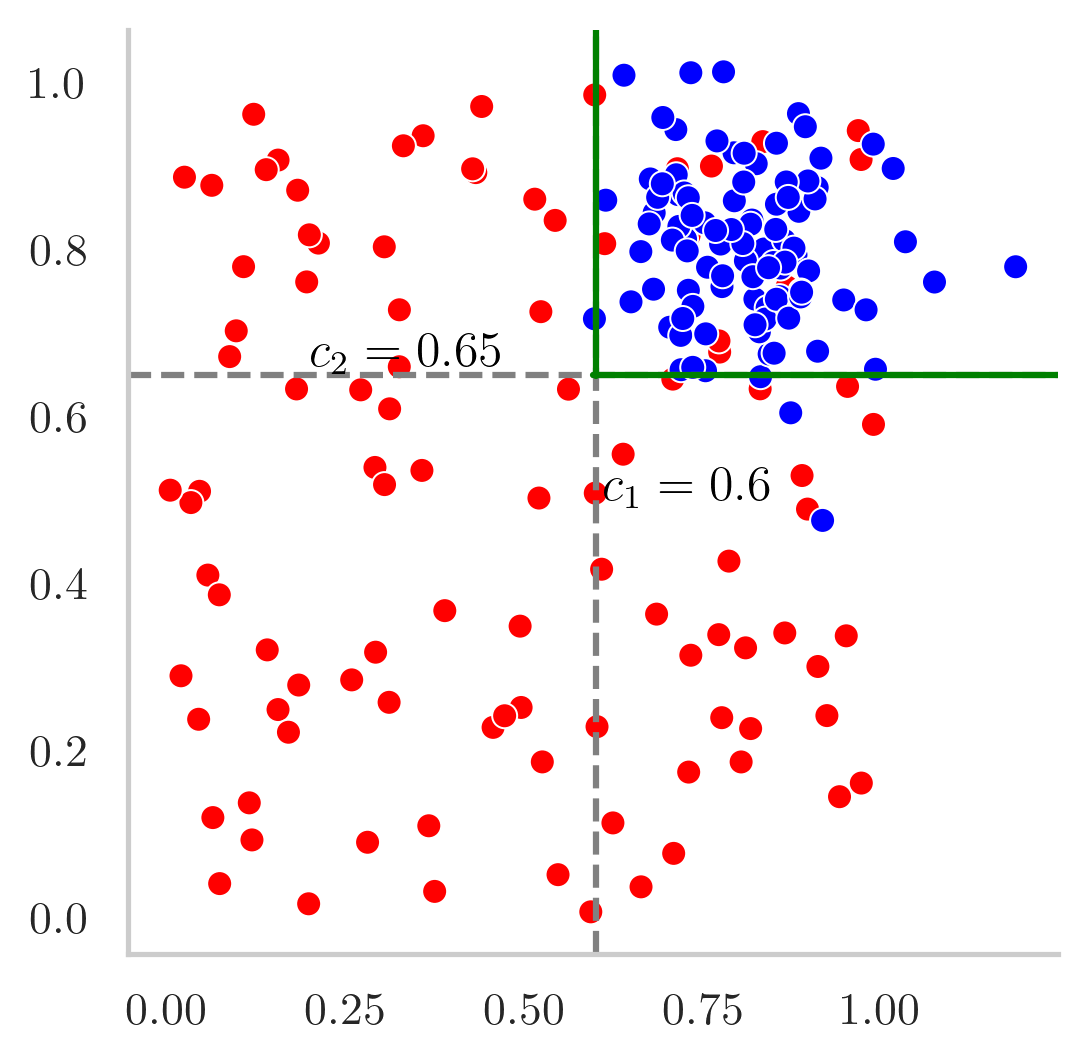
\includegraphics[width=\textwidth]{Images/ML/scatterPlot.png}
      \end{minipage}
\end{figure}
    
Finding the optimal set of partitions of a dataset is an NP-complete problem and therefore intractable for large datasets. To build a tree, a greedy approach must be adopted - meaning using a heuristic approach to find a satsifying solutions, e.g., successively choosing the most optimal step at each stage with no guarantee to find a global optimum instead of a local one. The chosen split is selected based on a defined \textit{cost} function as suggested in Equation \ref{eq:DTcost}.

\begin{equation}\label{eq:DTcost}
    (j^*, t^*) = \arg\min_{j\in \{1, ..., D\},\, t \in T_j} \min \left(\text{cost} (\{x_i, y_i : x_{ij} \leq t\}) + \text{cost}(\{x_i, y_i : x_j > t\}) \right)
\end{equation}
where $T_j$ is the set of possible thresholds, $x_j$, $y_j$ are the features and label (or regressive objective). For categorical variable, the inequality $x_j >< t$ is converted in a value equality $x_j == t$. The \textit{cost} function will depend on the objective of the tree, with the regression case typically using the error function \[cost(D) : \sum_{i\in D}(y_i - \bar{y})^2,\] and for a classification the loss would be one of the following:
\begin{itemize}
    \item \textit{Missclassification rate:} $\frac{1}{|D|} \sum_{i \in D} \mathbb{I}(y_i \neq \hat{y})$, where $D$ is the data in the leaf of the tree and $\mathbb{I}$ is the identity function: $\mathbb{I}(x) = 1$ if $x$ is True, else $0$. 
    \item \textit{Statistical entropy:} defining the class-condition probability as $\pi_c = \frac{1}{|D|} \sum_{i \in D} \mathbb{I}((y_i) \neq c)$, the entropy over the ($C$) classes is defined in Equation \ref{eq:statEntropy}
    \begin{equation}\label{eq:statEntropy}
        H(\vec{\pi}) = - \sum_{c=1}^C \pi_c \log \pi_c,
    \end{equation}
    with $\vec{\pi}$ being a vector ($\pi_1, \pi_2, ..., \pi_C$) with the class-condition probabilities as components.
    \item \textit{Information Gain:} an equivalent formulation to the entropy, where the gain in information that should be maximised is the relative change in entropy by adding a selection on feature $X_j$ over the current stage: 
    \[ \text{Gain}(X_j < t, Y) = H(Y) - H(Y | X_j < t) \]
    \item \textbf{Gini:} computes and minimises the expected error rate:
    \begin{equation}\label{eq:giniClass} 
        \sum_{c=1}^C \pi_c (1 - \pi_c).
    \end{equation}
\end{itemize}

The pseudocode algorithm to train a \gls{dt} with the update rule of Equation \ref{eq:DTcost} is summarised in Algorithm \ref{ag:DT}. 

\begin{algorithm}
    \caption{Recursive Procedure to Train a Decision Tree \cite{MurphyML}.}
    \begin{algorithmic}
    \Function{fitTree}{node, $D$, depth}
        \State $\text{node.prediction} \gets \text{mean}(\{y_i : i \in $D$\})$ 
        \State $(j^*, t^*, D_L, D_R) \gets \text{split}(D)$
        \If{\text{not worthSplitting}(\text{depth}, \text{cost}, $D_L$, $D_R$)}
            \State \Return node
        \Else
            \State node.left $\gets$ FITTREE(node, $D_L$, depth + 1)
            \State node.right $\gets$ FITTREE(node, $D_R$, depth + 1)
            \State \Return node
        \EndIf
    \EndFunction
    \end{algorithmic}
    \label{ag:DT}
\end{algorithm}

\gls{dt} can overfit a dataset: the model may tune itself to specific features of the training set that are not generalisable to any set samples from the true original distribution. Regularisation serves as an important step to avoid this often undesirable behaviour. For trees, a natural procedure to avoid overtraining is to interrupt the growth of the tree when it is no longer worth doing so - a criterion that is hard to decide \textit{a priori} - or to \textit{prune} the tree - removing nodes or branches that contribute little to the overall performance. A simpler way to regularise the performance by reducing the variance of the estimate of the model is to train several trees with different subsets of the data chosen randomly with replacement and aggregate the results into a single prediction. For example, for regression, one can take as output the average over each base learners: \[ y(x) = \frac{1}{N_l} \sum_{i=1}^{N_l} y_i(x),\] for $N_l$ base learner making prediction $y_i(x)$ given the input features $x$ and for classification select the class by majority voting. This statistical technique of using ensemble of predictors is referred to as \textit{bagging}. To further decorrelate the performance of the different predictors, these can be built on a subset of the input features and training datapoints, thereby forming a \textit{random forest}.

\subsection{Boosted Decision Trees}
A popular extension to the simple decision trees approach is to introduce the concept of \textit{boosting}, leading to a model referred to as a Boosted Decision Trees (\gls{bdt}) or \gls{mva} in particle physics. Boosting is a greedy algorithm leveraging a weak learner or predictor (e.g., a \gls{dt}) and applying it sequentially to weighted versions of the data, with a larger weight given to missclassified or miss-regressed datapoints, as per the use case. This method is hugely popular in data science, having earned the title \textit{``best off-the-shelf classifier in the world''} \cite{baggingML}. Two particularly useful approaches are adaptive boosting (AdaBoost) \cite{Adaboost} and gradient boosting \cite{gradientBoosting}, both combining an ensemble of $M$ weak learners $f_i$ ($i = 1, ..., M$) into a strong learner $F$: \[F(x) = \sum_{i=1}^M f_i(x).\] For the following discussion, the model is built using a training dataset $ \{(x_1, y_1), ..., (x_N, y_N)\}$ with input vectors $x_i \in \{\mathbb{R} \otimes \mathbb{D}\}^d$ of $d$ features that are real or discrete ($\mathbb{D}$) and $y \in \mathbb{R}^d$ is a $d$-dimension real vector that serves as output to be predicted by the model.

\subsubsection{AdaBoost}
AdaBoost combines the $M$ weak learners $f_i$ with adaptive weights $\alpha_i$ to improve the ensemble performance as \[F(x) = \sum_{i=1}^M \alpha_i f_i(x),\] where $F$ is the boosted model, and the successive boosting stages $F_T = \sum_{i=1}^{T \leq M} \alpha_i f_i(x)$ define stronger and stronger boosted variants of the model that combine weak learners $f_i$ with a weight $\alpha_i \in \mathbb{R}$. At each iteration $m$ of the training process ($m = 1, ..., M$), a weak learner $f_m$ is fitted to the training set to minimise a loss function $L(y_i, F_{m}(x_i))$. The loss in AdaBoost is the exponential loss on the datapoints of Equation \ref{eq:adaboosterror}:

\begin{equation}\label{eq:adaboosterror}
    L(y, F_m(x)) = \sum_{i=1}^N \exp\left(-y_i F_m(x_i)\right) = \sum_{i=1}^N \exp\left(-y_i (F_{m-1}(x_i) + \alpha_m f_m(x_i))\right),
\end{equation}
that the added new weak learner $\alpha_m f_m$ at step $m$ has to minimise: $(\alpha_m, f_m) = \arg \min_{(\alpha_m, f_m)} L(y, F_m(x))$. The typical case for AdaBoost is binary classification with $y_i \in \{-1, 1\}$ but the algorithm can be generalised to other cases \cite{MurphyML}. Equation \ref{eq:adaboosterror} can be re-expressed as: \[\sum_{i=1}^N w_{i,m} \exp\left(-\alpha_m y_i f_m(x_i)\right),\] where $w_{i,m} = \exp\left(-y_i F_{m-1}(x_i)\right)$ can be interpreted as a weight applied to the datapoint indexed by $i$ $(x_i, y_i)$ at step $m$ proportionaly to the error of the current strong learner. It can be shown that the weak learner $f_m$ minimising the optimisation objective at step $m$ is the one minimising the miss-classified weights sum error $\epsilon_m$ of the reweighted version of the dataset with weights $w_{i,m}$ \cite{MurphyML}, where: \[\epsilon_m = \sum_i w_{i,m} \mathbb{I}(y_i \neq f_m(x_i)).\] For the first time step $m = 1$, these weights are initialised to $1 / N$. The weights are then updated to \[w_{i,m+1} = w_{i,m} e^{-\alpha_m y_i f_m(x_i)},\] and renormalised so that $\sum_i w_{i, m+1} = 1$ before being assigned to each training sample $i$ for the next step. The weak learner can be combined with the strong learner using an optimal weight $\alpha_m$ found by minimising the loss $L$ of the combined learner: \[\alpha_m = \frac{1}{2} \log \frac{1 - \epsilon_m}{\epsilon_m},\] giving the overall update rule of Equation \ref{eq:updateOverall}:
\begin{equation}\label{eq:updateOverall}
    F_m(x) = F_{m-1}(x) + \alpha_m f_m(x),
\end{equation}
combining the new weak learners $f_m$ with optimal weight $\alpha_m$ to the current strong learner. The AdaBoost algorithm is summarised in Algorithm \ref{algo:adaboost}.

\begin{algorithm}
    \caption{Adaboost for Binary Classification with Exponential Loss \cite{MurphyML}}
    \label{algo:adaboost}
    \begin{algorithmic}
    \State Initialise weights: $w_{i,1} = \frac{1}{N}$, where $N$ is the number of samples.
    \For{$m = 1$ to $M$}
        \State Minimise $\epsilon_m = \sum_i w_{i,m} \mathbb{I}(y_i \neq f_m(x_i))$ on training set with weights $w_{i,m}$ to find $f_m(x)$.
        \State Compute $\alpha_m = \frac{1}{2} \log\left(\frac{1 - \epsilon_m}{\epsilon_m}\right)$.
        \State Update weights: $w_{i,m+1} \leftarrow w_{i,m} \, \exp(-\alpha_m y_i f_m(x_i))$ and renormalised $\sum_i w_{i, m+1} = 1$.
    \EndFor
    \State \Return $F(x) = \sum_{m=1}^M \alpha_m f_m(x)$
    \end{algorithmic}
\end{algorithm}

\subsubsection{Gradient boosting}
Gradient boosting is a generic approach which, contrary to AdaBoost, does not require a specific derivation for each loss function. The objective is to minimise the empirical risk, the expected value of the loss function $L$ on the training set as shown in Equation \ref{eq:empRisk} 
\begin{equation}\label{eq:empRisk}
    \hat{f}  = \arg \min_f \mathbb{E}_{x,y} L(y, f(x))
\end{equation}
where $f(x) = (f(x_1), ..., f(x_N))$ is the output of the learner on the whole training set. As the name suggests, the approach leverages gradient descent to find the optimal $\hat{f}$. At step $m$, the gradient of the loss $L$ is evaluated at $f = f_{m-1}$ as \[ g_{i,m} = \left[ \frac{\partial  L(y_i, f(x_i))}{\partial f(x_i)} \right]_{f= f_{m-1}}, \] which is then used to update the learner with a step \[ f_m = f_{m-1} - \alpha_m g_{m},\] where $g_m$ = ($g_{1, m}, g_{2, m}, ..., g_{N,m}$) and the step-length $\alpha_m$ is chosen to minimise the residual loss $L(y, f_{m-1}$ $- \alpha_m g_{m})$. This implements functional gradient descent, and leads the model to fit the $N$ datapoints of the set. This procedure naturally leads to overfitting the training set, an undesirable feature that is remedied by using a weak learner to approximates the negative gradient. In the specific case of gradient boosted decision trees, at step $m$ a decision tree $h_m(x)$ is fitted to the pseudo-residuals $g_{i,m}$. This \gls{dt} $h_m$ at step $m$ defines $J_m$ disjoint regions through its leaves with predictions $b_{jm}$ in each $j = 1, ... J_m$ region: \[ h_m(x) = \sum_{j=1}^{J_m} b_{jm} \textbf{1}_{R_{jm}}(x),\] where $\textbf{1}_{R_{jm}}(x)$ is the indicator function - equals to 1 when $x \in R_{jm}$ and 0 otherwise. The update to the model is chosen so that: \[f_m(x) = f_{m-1} + \alpha_m h_m(x),\] with $\alpha_m$ selected by minimising the empirical risk of the updated model: \[ \alpha_m = \arg \min_{\alpha} \sum_{i=1}^N L(y_i, f_{m-1}(x_i) + \alpha h_m(x_i)).\]

\begin{algorithm}
    \caption{Gradient Boosting \cite{MurphyML}}
    \label{algo:gradient_boosting}
    \begin{algorithmic}
    \State Initialise $f_0(x) = \arg\min_\alpha \,\sum_{i=1}^N L(y_i, \alpha)$
    \For{$m = 1$ to $M$}
        \State Compute the gradient residual for each $i= 1, ..., N$: $g_{i,m} = -\left[\frac{\partial L(y_i, f(x_i))}{\partial f(x_i)}\right]_{f(x_i) = f_{m-1}(x_i)}$
        \State Train weak learner $h_m$ on the dataset $\{(x_i, g_{i,m})\}_{i=1}^N$
        \State Compute $\alpha_m$ by minimising $\sum_{i=1}^N L(y_i, f_{m-1}(x_i) + \alpha h_m(x_i))$
        \State Update $f_m(x) = f_{m-1}(x) + \nu \alpha_m h_m(x)$
    \EndFor
    \State \Return $f(x) = f_M(x)$
    \end{algorithmic}
\end{algorithm}

The full algorithm for Gradient Boosting is presented in Algorithm \ref{algo:gradient_boosting}, where the update rule is added a \textit{learning rate} hyperparameter $\nu$ to introduce regularisation and reduce the risk of overfitting. By keeping $0 < \nu \leq 1$, it limits the ability of the model to fully adapt to the training error, thereby improving generalisation. The price is a slower updating of the model and therefore a more demanding computational complexity. Further regularising techniques are bootstrap aggregation - training each weak learner on a random subset of the data -, limiting the number of leaves, or more generally penalising model of larger complexity - removing branches that do not reduce the loss by a minimal amount. \\

\gls{bdt} resist better to overtraining thanks to the regularisation effect of boosting and the different techniques described in this section. Unfortuntaly, an undiserable feature of boosting is the loss of direct interpretability of the decision-making but this is more than met by an appreciable \textit{boost} in performance of the underlying model. An interesting property exhibited by all tree-based algorithms and many \gls{ml} approaches is the ease to quantify the impact of a specific feature on the result. This technique of \textit{feature importance} assigns a score to each input feature, typically the Gini importance of Equation \ref{eq:giniClass}, quantifying the reduction in entropy obtained by adding a feature, or the Shapley value, measuring the average marginal contribution of each feature.  

\paragraph{Pros:}
\begin{itemize}
    \item \textit{Adaptability to Different Distributions:} Boosting algorithms, such as AdaBoost and Gradient Boosting, can adapt well to different types of data distributions and can capture non-linear relationships in the data.
    \item \textit{High Accuracy:} \gls{bdt} easily achieve high accuracy in both classification and regression tasks, making them suitable for a wide range of applications.
    \item \textit{Ensemble Learning:} The boosting technique leverages ensembling by combining multiple weak learners to create a strong learner, improving overall model performance.
    \item \textit{Robustness to Overfitting:} Boosting helps mitigate overfitting, enhancing the  generalisation of the model to unseen data. \gls{bdt} typically perform reasonably well out-of-the-box. 
    \item \textit{Feature Importance:} \gls{bdt} provide a measure of feature importance, aiding in feature selection and interpretability of the model.
\end{itemize}

\paragraph{Cons:}
\begin{itemize}
    \item \textit{Sensitivity to Noisy Data:} \gls{bdt} can be sensitive to noisy data and outliers, potentially leading to overfitting.
    \item \textit{Computational Complexity:} Training multiple weak learners sequentially can be computationally expensive, especially for large datasets or deep tree structures.
    \item \textit{Parameter Tuning:} \gls{bdt} still require some fine-tuning of the hyperparameters, such as learning rate and tree depth, for optimal performance.
    \item \textit{Black Box Nature:} The ensemble nature of boosted decision trees make them somewhat of a black box, sacrifing the perfect interpretability of \gls{dt} for the sake of performance.
\end{itemize}

\subsection{Artificial Neurons}
The Artificial Neuron, also called the \textit{perceptron} by its inventor Frank Rosenblatt in his seminal 1958 paper \cite{rosenblatt1958perceptron}, is the logical gate that underpins most \gls{dl} models. Notably, a \gls{mlp} - also called a \gls{dnn} - is a stacking of layers of artificial neurons. Inspired by biological principles, the perceptron, as shown in Figure \ref{fig:annModel}, accepts multiple intputs and gives as output 1 if the combination of inputs exceeds a certain modifiable threshold, otherwise giving 0. This combination accepts weights to scale the input which, remarkably, can be adjusted during a training phase if the output of the perceptron is incorrect. Artificial neurons are a direct generalisation of this very principle, with the output no longer being thresholded but applied a chosen function $f$ after being added a learnable bias term $b$. 

\begin{figure}[h!]
    \center
    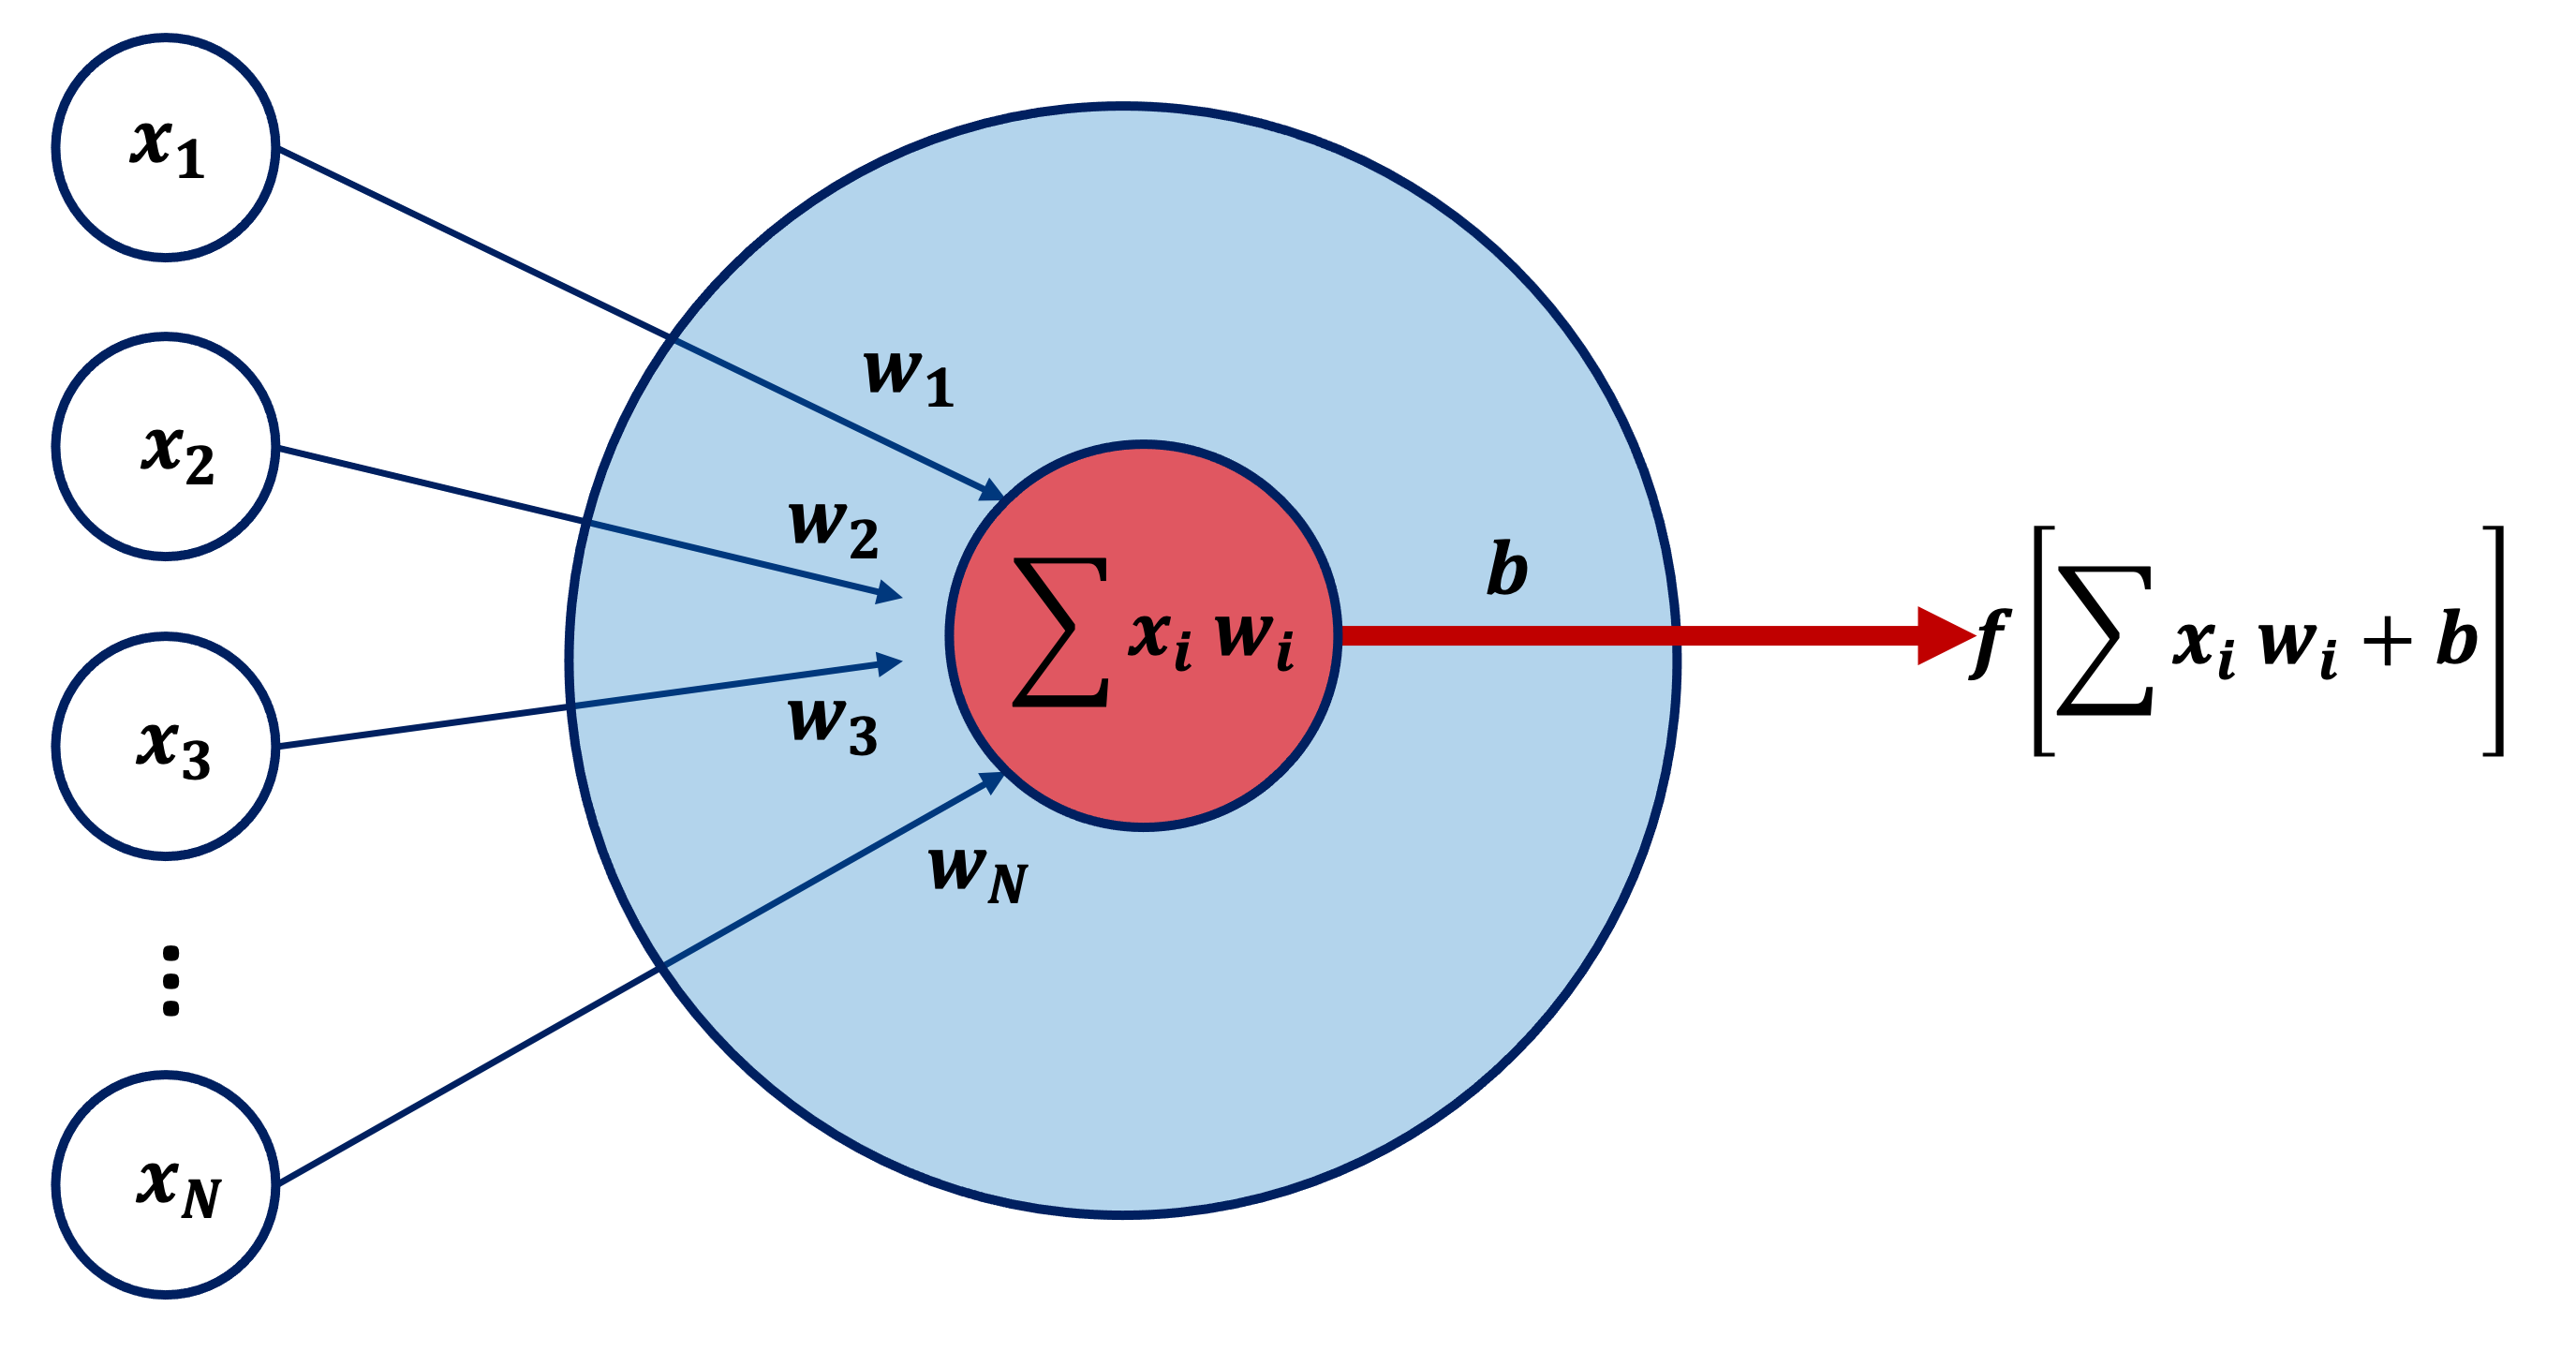
\includegraphics[scale=0.4]{Images/ML/ann.png}
    \caption{Schematics of a perceptron or an artifical neuron: the inputs $x_i$ ($i= 1, ..., N$) is multiplied by learnable weights $w_i$, summed and added a bias $b$ before being passed to an output function $f$.} 
    \label{fig:annModel}
\end{figure}

In this thesis, a \textit{perceptron} shall refer to a single artificial neuron, which is equivalent to a logistic regression model. The interest of the artificial neuron stems from a significant theoretical result: stacks of artificial neurons are \textit{universal function approximator} \cite{universalFuncApproxNN,HORNIK1989359}, as is shown in the next section on deep neural network. This theoretical result is built on a mathematically advantageous function choice for $f$: the sigmoid $\sigma$, defined in equation \ref{eq:sigmoid} and shown in Figure \ref{fig:sigmoid}:
\begin{wrapfigure}{r}{0.5\textwidth}
    \begin{center}
        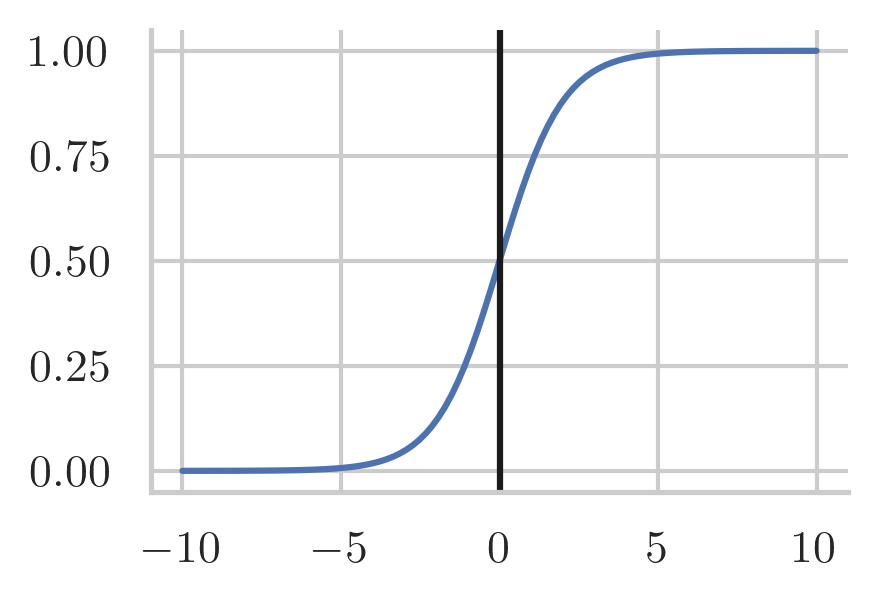
\includegraphics[width=0.35\textwidth]{Images/ML/sigmoid.png}
        \caption{The sigmoid function $\sigma$.} 
        \label{fig:sigmoid}
    \end{center}
\end{wrapfigure}

\begin{equation}\label{eq:sigmoid}
    \sigma(x) = \frac{1}{1 + e^{-x}}.
\end{equation}

Thanks to its property to map the range of real numbers to the [0, 1] range, this activation function is often used for numerical stability and to map some input to a probability distribution. A practical mathematical property of the sigmoid that is particularly relevant for \gls{dl} is the ease to compute its derivative: \[\sigma^\prime(x) = \sigma(x) (1- \sigma(x)).\]

The power of the artificial neuron comes from its ability to be efficiently combined into a well-ordered structure with powerful representation power. For an input $x \in \mathbb{R}^d$, a neuron individually applies an affine transformation $W_i^T x + b_i$, where $W_i \in \mathbb{R}^d,\,b_i \in \mathbb{R}$ are the weights and bias of the neuron $i$, that is passed through an activation function $f$ for a total output of a single neuron $f(W_i^T x + b_i)$. Combining these operations, as shown in the next section, leads to a well-structure mathematical model that has the power to represent all well-behaved continuous functions. 

\subsection{Deep Neural Networks}
A Deep Neural Network (\gls{dnn}), also called Multilayer Perceptron (\gls{mlp}), \gls{ann}, \gls{nn}, or feed-forward neural network, is made by stacking layers of artificial neurons as shown in Figure \ref{fig:neuralnet} Each neuron in a layer receives as input the output of each neuron of the previous layer, and connects to each neuron of the next layer. Layers of artificial neurons that are placed between the input and output are said to be \textit{hidden layers}. The particularlity of the design of this architecture is that layers of neurons connect to all neurons of the next layers only, defining a feed-forward computation graph from input $x$ to output $y$. Mathematically, a single layers at depth $i$ with $m$ units given as input the previous layer of dim $n$ at depth $i-1$ computes the  transformation of Equation \ref{eq:feedforward}

\begin{equation}\label{eq:feedforward}
    a^i = f^i\left({W^i}^T a^{i-1} + b_i\right),
\end{equation}
where $W^i \in \mathbb{R}^{m \times n}$ is the matrix of weight of layer $i$ - one row per unit of layer $i$, one column per unit of layer $i-1$, $b_i \in \mathbb{R}^m$ is the vector of bias, one per unit of layer $i$, $f^i$ is the activation function of layer $i$, and $a^{i-1} \in \mathbb{R}^n$ are the $n$ activated output of layer $i-1$. Note that strictly speaking the activation could be different for the units of the layer but is often unique per layer to accelerate matrix computations with vector operations.

\begin{figure}[h!]
    \center
    \begin{minipage}[l]{0.38\textwidth}
        \caption{A deep neural network with $d$ layers of width $m$, $l$ ..., $k$. Each artificial neuron, represented by a ball of darkening blue along depth, computes an affine transformation of the input of the layer followed by an activation function. The input of the \gls{dnn} is $x$ and the output is $y$.} 
    \label{fig:neuralnet}
      \end{minipage}
      \begin{minipage}[c]{0.6\textwidth}
        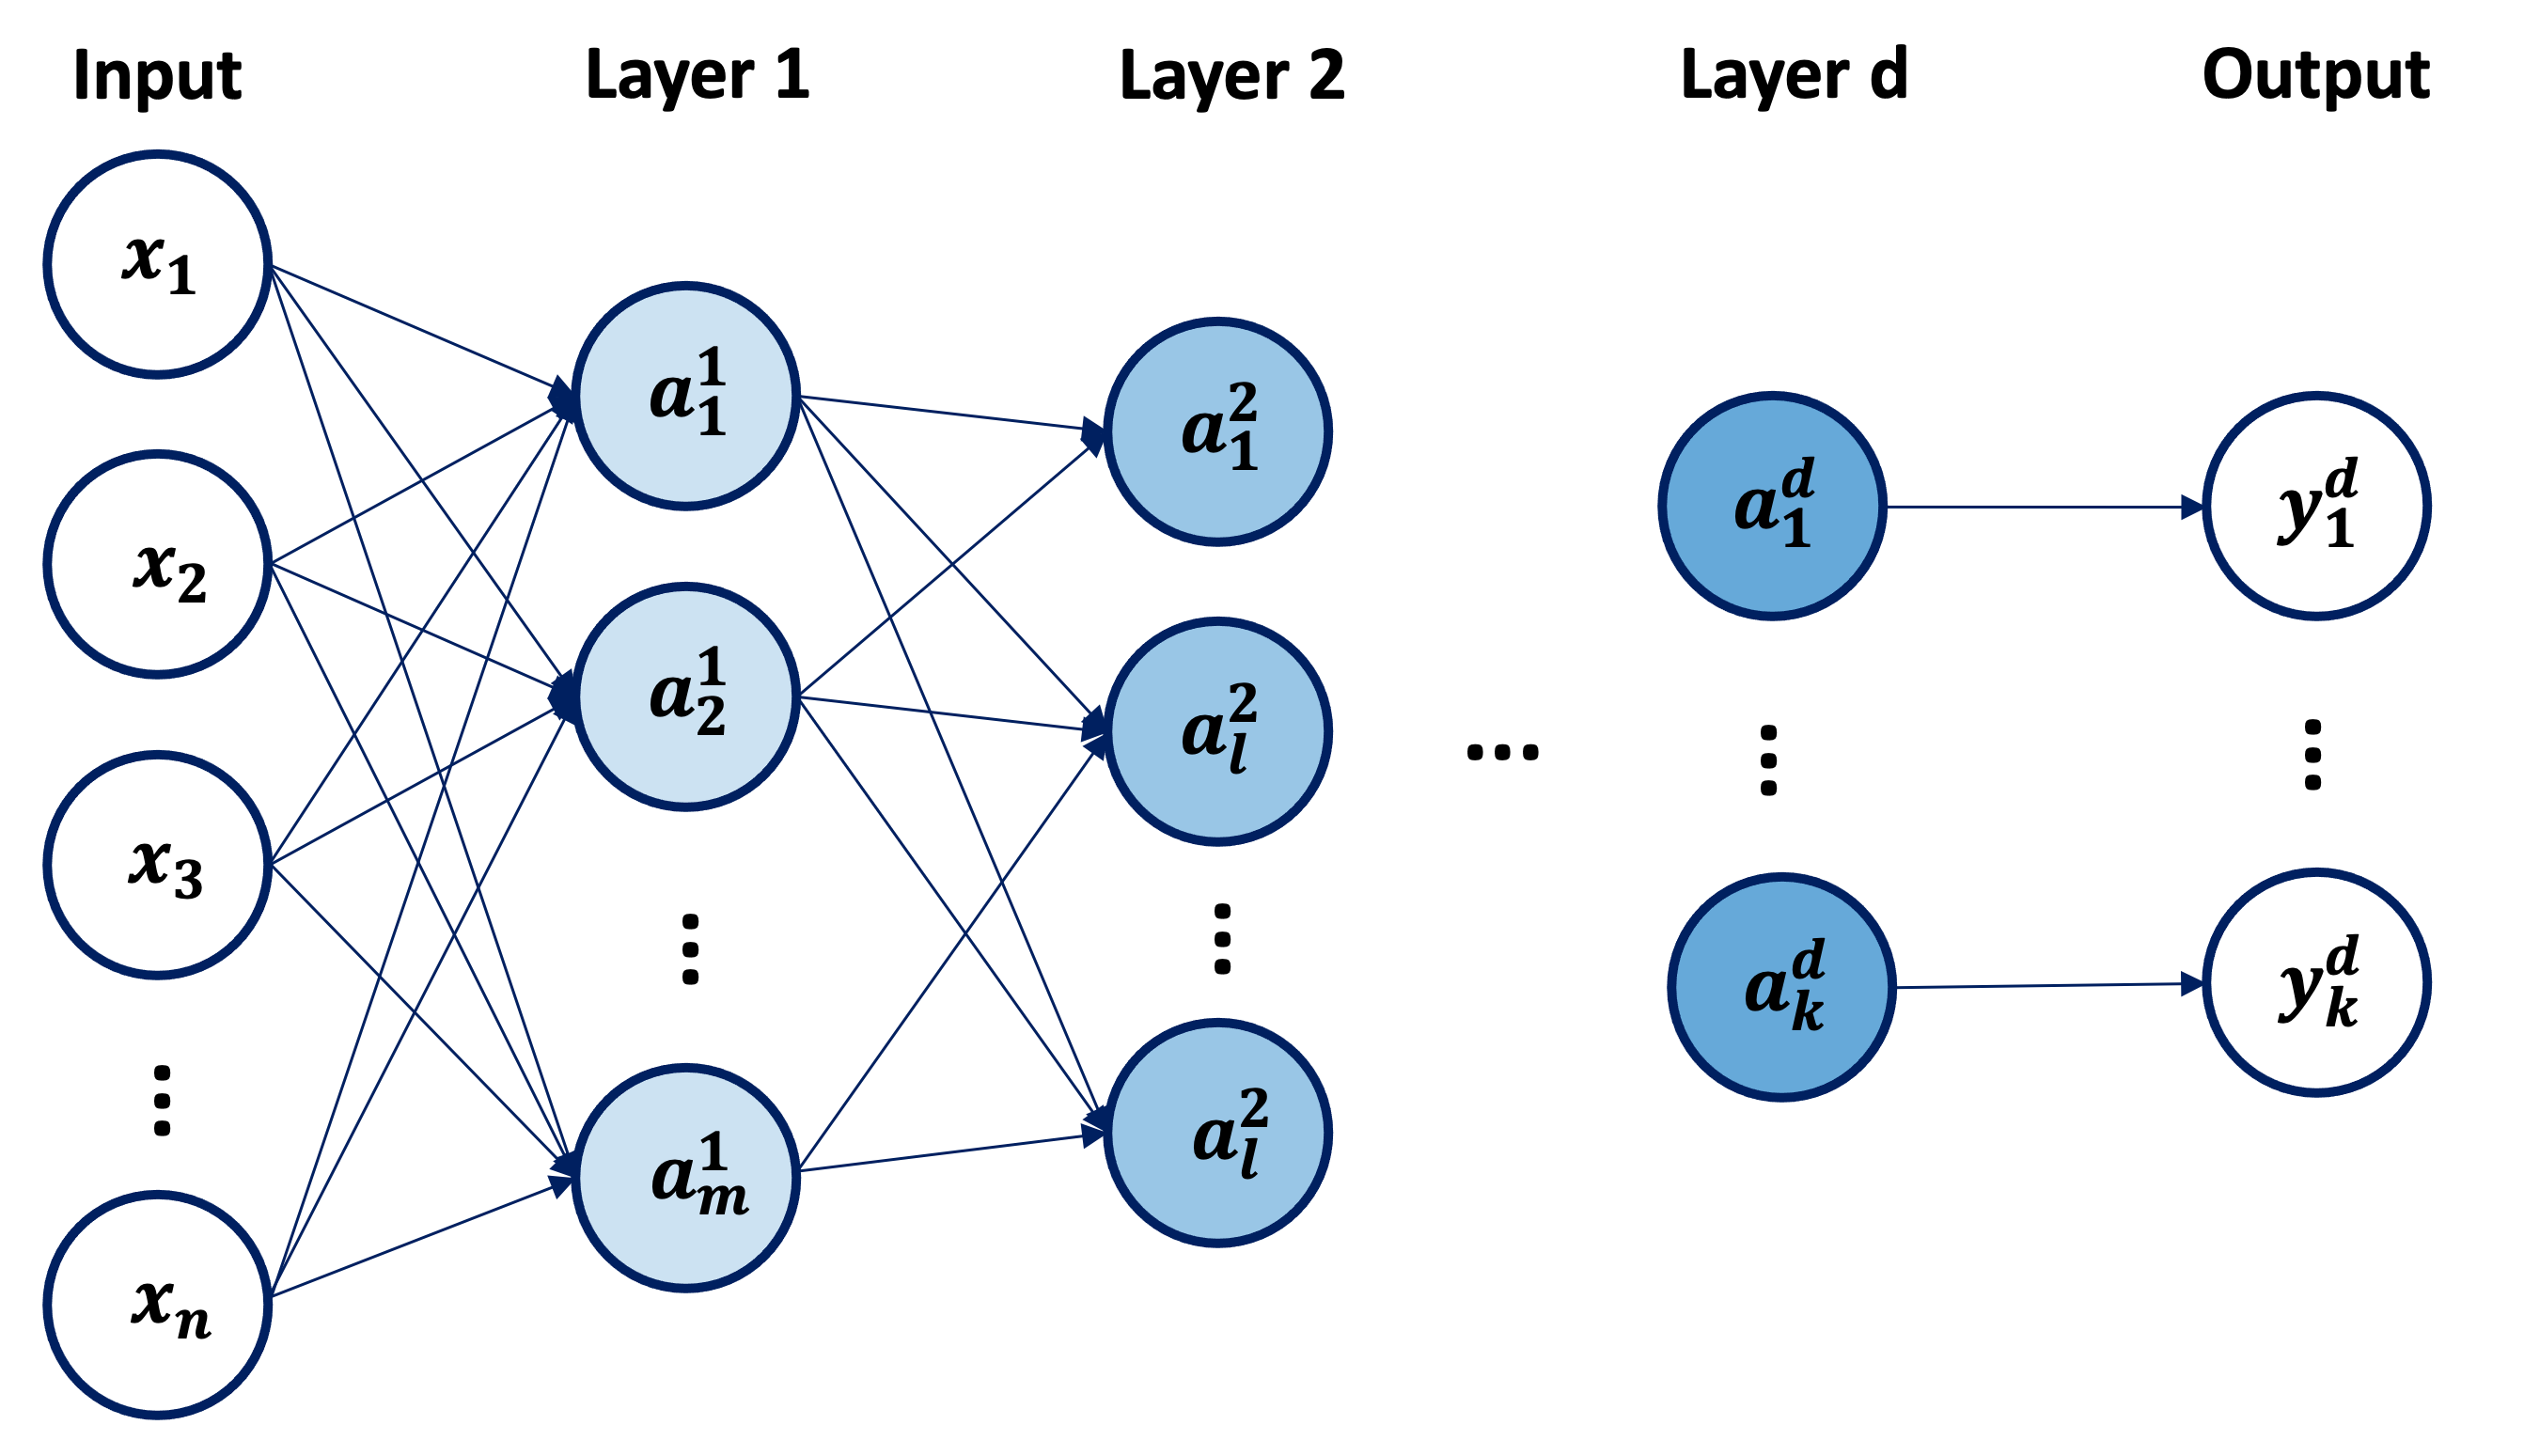
\includegraphics[width=\textwidth]{Images/ML/neuralnet.png}
      \end{minipage}
\end{figure}

Neural networks implement a system computing combination of Equation \ref{eq:feedforward}. A powerful theoretical motivation for neural networks stems from the fact they are Universal Function Approximator. This theorem, or rather family of theorem depending on the type of activation $f$ considered, establishes that neural network built with appropriate activation functions are able to approximate most well-behaving functions. The most famous such theorem states \cite{universalFuncApproxNN,HORNIK1989359}:

\paragraph{Theorem:} \textit{Let $C([0, 1]^n)$ denote the set of all continuous function $[0, 1]^n \rightarrow \mathbb{R}$ and $\sigma$ be any sigmoidal activation function. Then the finite sum $f(x) = \sum_{i=1}^N \alpha_i \sigma(w_i^T x + b_i)$ is dence in $C([0, 1]^n)$. In other words, given any $f \in C([0, 1]^n)$ and $\epsilon > 0$, $\exists$ a sum $G(x)$ of the above form for which: \[ G(x) - f(x) < \epsilon \quad \forall x \in [0, 1]^n.\]}

The statement of the theorem essentially is that any function defined over the $n$-dimensional unite hypercube $[0, 1]^n$ can be approximated by an arbitrarily wide neural network. This result only requires $\sigma$ to be sigmoidal or discriminatory in the sense:
\begin{equation}
    \sigma(x) \rightarrow
    \begin{cases}
        1 \text{ if } x \rightarrow \infty,  \\
        0 \text{ if } x \rightarrow -\infty,
    \end{cases}
\end{equation}
which is, for example, satisfied by the sigmoid function. Interestingly, similar theorems were derived for other important activation function commonly used in \gls{dl}, for example for ReLu in \cite{universApproximator-Relu}. Many flavours of \gls{dnn} exist with different functions used. An important theoretical result is the requirement for the output function applied to the artificial neuron to possess some degree of \textit{non-linearity}. A neural network with strictly linear functions can indeed be seen to collapse to a linear regression model. Such a function, when applied to the output of an artificial neuron, is said to \textit{activate} it and is hence called \textit{activation functions}. The most popular such functions, shown in Figure \ref{fig:commonAct}, are:
\begin{itemize}
    \item The sigmoid function of Equation \ref{eq:sigmoid}.
    \item The hyperbolic tangent function $tanh = \frac{e^x - e^{-x}}{e^x + e^{-x}}$.
    \item The \gls{relu} function of Equation \ref{eq:relu}
    \begin{equation}\label{eq:relu}
        \text{ReLu}(x) = \text{max}(0, x),
    \end{equation}
    note that the non-linearity here is strictly between positive and negative inputs, making this activation function one of the simplest that can be leveraged in \gls{dnn} for universal function approximation. The deriviative of this function is indeed particularly easy to compute. A generalisation of \gls{relu} called leakyReLU introduces a linear function in the negative range as leakyReLu $= \max(\alpha x, x)$, with $\alpha \in [0, 1[$. 
    \item The Exponential Linear Unit (ELU) function, shown in Equation \ref{eq:elu}, modifies the Leakage \gls{relu} in the negative domain while keeping the saturation property:
    \begin{equation}\label{eq:elu}
        \text{Elu}(x) = 
        \begin{cases}
            x \quad \text{ if } x >= 0, \\
            \alpha (e^x - 1) \text{ otherwise},
        \end{cases}
    \end{equation}
    where the a hyperparameter $\alpha > 0$.
    \item The softmax function. For an $x \in \mathbb{R}^n$, the softmax return a vector softmax$(x) = [..., \frac{e^{x_i}}{Z}, ...]$ (for $i= 1, ..., N$), where $Z = \sum_i e^{x_i}$. For a 2-dimensional $x$, the softmax is equivalent to the sigmoid function. In $n$-dimension, it maps each entry of $x$ to the range $[0, 1]$ and guarantees $\sum_i $softmax$(x)_i = 1$. The softmax is therefore  helpful to define probability distributions over multidimensional outputs.
\end{itemize}

\begin{wrapfigure}{R}{0.5\textwidth}
    \begin{center}
        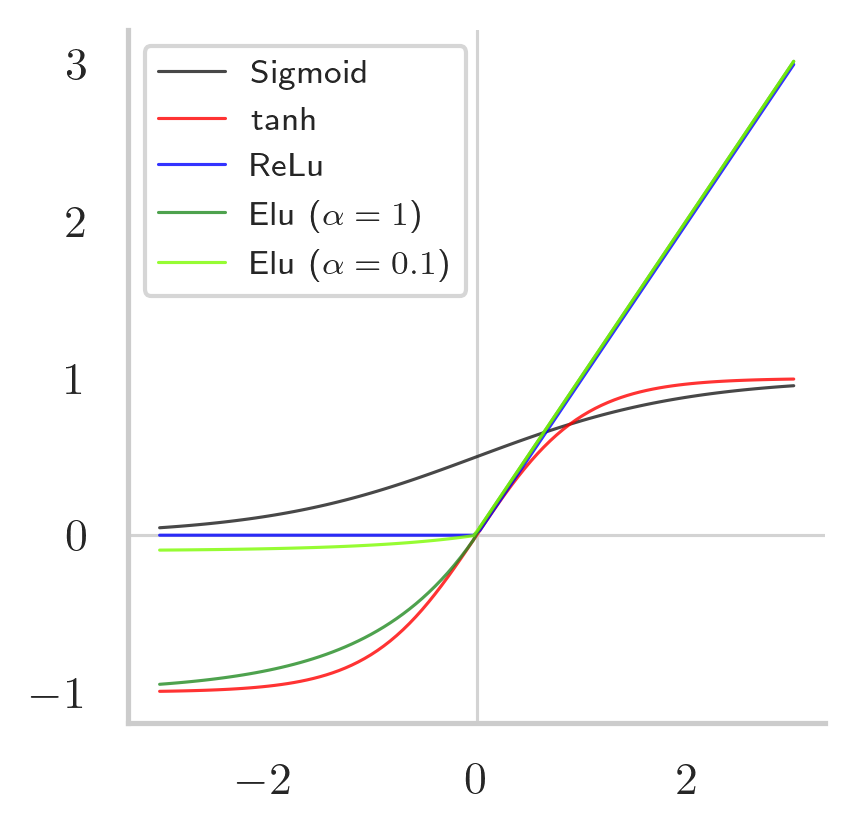
\includegraphics[width=0.45\textwidth]{Images/ML/activations.png}
        \caption{The most common non-linear activations used in deep learning.} 
        \label{fig:commonAct}
    \end{center}
\end{wrapfigure}

Many more functions have been defined in the field of \gls{ai}, with none seemingly offering a clear advantage over the ones listed here. The sigmoid is no-longer the choice of reference, due to its tendency to quickly saturates - meaning its gradient for large positive or negative input values vanishes in the sense that it tends to 0. The hyperbolic tangent $tanh$ offers larger gradients thanks to its [-1, 1]range with steeper curvature and is often the activation of choice for autoregressive architecture, such as the \gls{rnn}. The \gls{relu} function is the most widely used activation function as its derivative is extremelly efficient to compute - 1 for positive inputs and otherwise 0 - and does not suffer from vanishing gradients for positive values. Its fixed 0-value for negative input is a double edge sword: on one side, it helps the network regularises itself by deactivating neurons, on the other it could let some neurons being stuck in \textit{off}-mode if the weights are such that its pre-activation value is always negative for the input data. For this reason, it is important to correctly initialises the weights of a \gls{dnn}. An easy work around this limitation is the leakyReLu and the Elu activations, which both introduce some leakage in the negative value as controlled by a parameter $\alpha$.\\
While the Universal Function Approximator theorem gives a powerful endorsment of \gls{dl} networks, it does not state how to derive such a netowrk to fit a specific function. The task of choising the right architecture depthwise and widthwise and the correct weights and biases must be approximated by a learning strategy updating the weights and biases to reduce the error between the output and a given target. Many other data models are also Universal Function Approximators and what sets appart \gls{dl}-like models that are built on artificial neurons is the simplicity of the procedure to update their weights: thanks to their nice computational structure, under a reasonable choice of activation functions for each layer, the network is \textit{differentiable}. This means a gradient can be computed on a function measuring the difference between the target $y$ and the output $\hat{y}$ - often called a loss function when it should be minimised or a reward function when it is to be maximised - and \textit{backpropagated} across each neuron of each layer to give a local update to be applied to each individual weight and biases. The recent rise of \gls{dl} in \gls{ai} can be traced back to improvements in making this backpropagation of the gradients with publicaly available software, such as PyTorch \cite{pytorch} and TensorFlow \cite{tensorflow2015-whitepaper}, implementing efficient algorithm to perform this essential step. \\
One of the main difficulty in training a neural network is the non-convexity of the loss function as a function of the model parameters. The large number of parameters typically implemented by neural networks require large dataset to correctly assign values to the parameters without suffering from overtraining - the property to only correctly describe the data of the training set without being able to generalise the performance to data not seen during the training phase. There are two main difficulties encountered when optimising a neural network: the non-convexity of the objective function means saddle points and local minima are typically abundant and the computational complexity due to the large number of parameters makes a single update using a large dataset expensive. To circumvent these, the \textit{backpropagation} algorithm of Algorithm \ref{ag:backpropagation} is used \cite{backprop}.

\begin{algorithm}
    \caption{Backpropagation Algorithm}
    \begin{algorithmic}
    \Function{Update}{$x$, $y$, $N$, $\mathcal{L}$}
        \State Forward step: propagate input $x$ through network $N$ to get prediction $\hat{y}$
        \State Loss: compute the loss or reward of $N$: $\mathcal{L}(y, \hat{y})$
        \While{$\exists$ a layer with no gradients}
            \State Take right-most layer required a gradient
            \State Take input of layer to its right 
            \State Using the chain-rule of calculus, propagate gradient of next layer to that of current layer
            \State Store the gradient at the layer
        \EndWhile
    \EndFunction
    \end{algorithmic}
    \label{ag:backpropagation}
\end{algorithm}

In summary, the backpropagation algorithm serves as an effective way to compute \[ \frac{\partial\mathcal{L}(\theta)}{\partial\theta} = \sum_{i=1}^N \frac{\partial l(\theta)}{\partial\theta},\] 
where $\theta$ encapsulates all parameters of the model and there are $N$ datapoints, with a per datapoint loss of $l$. 
The backpropagation algorithm starts with a forward pass through the network: \[ x \xrightarrow{\times W^1 + b^1} z^1 \xrightarrow{f^1()} a^1 \xrightarrow{\times W^2 + b^2} z^2 \xrightarrow{f^2()} a^2 \xrightarrow{\times W^3 + b^3} ... \xrightarrow{\times W^d + b^d} a^d = \hat{y},\] the loss is then computed $\mathcal{L}(y, \hat{y} | W^1, b^1, W^2, b^2, ..., W^d, b^d)$ before computing the gradient of each layer by starting from the right:\[\text{grad}_{W^d, b^d} = \nabla_{W^d, b^d} \mathcal{L} \rightarrow \text{grad}_{W^{d-1}, b^{d-1}} = \nabla_{W^{d-1}, b^{d-1}} \text{grad}_{W^d, b^d} \rightarrow ... \rightarrow \nabla_{W^{1}, b^1} \text{grad}_{W^2}, \]
where the operation $\text{grad}_{W^{d-1}, b^{d-1}} = \nabla_{W^{d-1}, b^{d-1}} \text{grad}_{W^d, b^{d}}$ implies a use of the chain rule to obtain the local gradient, based on information already obtained. In the context of \gls{dl}, the chain rule of multivariate calculus offers a transformation:
\begin{equation}
    \frac{\partial h}{\partial x} = \frac{\partial h}{\partial z}\frac{\partial z}{\partial x},
\end{equation}
for a function $h: \mathbb{R}^n \rightarrow \mathbb{R}^m$, composiong two functions $h = g \circ f$ defined as $f: \mathbb{R}^n \rightarrow \mathbb{R}^k$, $g: \mathbb{R}^k \rightarrow \mathbb{R}^m$, with $x \in \mathbb{R}^n$ and $z = f(x) \in \mathbb{R}^k$. Two types of updates are necessary: 
\begin{itemize}
    \item For a layer $l$, the activation can be unpacked: \[\frac{\partial l}{\partial z^l} = \frac{\partial l}{\partial a^l} \frac{\partial a^l}{\partial z^l}\]
    \item For a layer $l$ having access to next layer $l+1$ $(\frac{\partial l}{\partial z^{l+1}})$: \[\frac{\partial l}{\partial z^l} = \frac{\partial l}{\partial z^{l+1}} \frac{\partial z^{l+1}}{\partial z^l} = \frac{\partial l}{\partial z^{l+1}} \frac{\partial z^{l+1}}{\partial a^l} \frac{\partial a^l}{\partial z^l}, \] but since $z^{l+1} = W^{l+1}a^l + b^{l+1}$, this reduces to:\[\frac{\partial l}{\partial z^l} = \frac{\partial l}{\partial z^{l+1}} W^{l+1} \frac{\partial a^l}{\partial z^l}, \]

    \item Combining the two above, we can compute $\frac{\partial l}{\partial z^l}$ for each layer in backward order. One thus now requires the derivative with respect to the per-layer weights: \[\frac{\partial l}{\partial W^l} = (a^{l-1} \frac{\partial l}{\partial z^l})^T,\] 
    
    for the weight matrix - an outer product between a row vector $\frac{\partial l}{\partial z^l}$ and a column vector $a^{l-1}$. For the bias: \[\frac{\partial l}{\partial b^l} = \frac{\partial l}{\partial z^l},\] the result is directly obtained from the row vector. 
\end{itemize}

Once all the gradients are locally available, the next step is to update all the parameters to reduce the loss by taking a step in the direction opposed to the gradient, giving the largest reduction in loss. For example for a specific parameter $w_{ij}$ at training step $t+1$:
\begin{equation}\label{eq:gradientdescent}
    w^{T=t+1}_{ij} \leftarrow w^{T=t}_{ij} - lr \times \text{grad}\left[w^{T=t}_{ij}\right],
\end{equation}
where the \textit{learning rate} $lr$ controls how large a step is taken in the opposite direction of the gradient. Since the gradient of the earlier layers will be derived from the gradient of later layers, it is important for the gradients to respect some numerical stability to avoid the risk of vanishing gradient ($\rightarrow$ 0) or exploiding gradients ($\rightarrow \infty$). This requires some care in the architecture choice and might motivate the use of a specific activation function over another. Note that strictly speaking, the activation function needs not be a continuous differentiable function ($C^1$), as the existence of a right or left derivative is sufficient, hence the function should at least be continuous ($C^0$). \\
Concerning the loss function $\mathcal{L}$, there is a lot of freedom in how to set it up - although it should be differentiable - and some typical choices are:
\begin{itemize}
    \item The cross-entropy loss function - also called the logistic loss - is based on the notion of entropy, as defined in Equation \ref{eq:statEntropy}, and is often used to assign probabilities in a classification with $c$ classes: \[ -y_i \log\hat{y}_i,\] where $y_i$ is the real label of the datapoint and $\hat{y} \in [0, 1]^C$ is the model prediction, respecting $\sum_i \hat{y}_i = 1$. Given the requirements on the output, it is typically combined with a softmax. 
    \item the Mean Squared Error (MSE): \[\frac{1}{N}\sum_i^N (y_i - \hat{y}_i)^2.\] 
    \item the Mean Absolute Error (MAE): \[\frac{1}{N}\sum_i^N |y_i - \hat{y}_i|.\]
\end{itemize} 
To regularise the model, it is common to add terms to the loss function called \textit{regulariser} in order to restric the model weights to a certain size. This can be achieved by adding to the loss $\mathcal{L}$ an L2-penalty \[\lambda \sum_i w_i^2,\] on the sum of the squared values of the weights, or an L1-penalty \[\lambda \sum_i |w_i|,\] where this last approach using the absolute value has the nice additional feature to make the network sparse - meaning to set un-necessary weights at 0. The amount of regularisation is controlled by the hyperparameter $\lambda$. Further regularisation can be obtained by randomly dropping out some connexions of the network during training, a technique called \textit{dropout} and controled by the dropout probability $p$ to incude an artificial neuron or not.

\paragraph{Pros:}
\begin{itemize}
    \item \textit{Universal Function Approximators:}
    Feedforward networks, particularly deep ones, are known to be universal function approximators. They can approximate any continuous function to arbitrary precision given sufficient hidden units and appropriate activation functions.
    \item \textit{Flexible Architecture:} The architecture of feedforward networks is flexible, allowing for customization in terms of the number of layers, the number of neurons in each layer, and the choice of activation functions. This flexibility makes them suitable for various tasks.
    \item \textit{Feature Learning:} Feedforward networks can automatically learn hierarchical representations of features from the input data. This is beneficial for tasks where the underlying patterns are complex and not easily captured by handcrafted features.
    \item \textit{Non-linearity Handling:} By introducing non-linear activation functions, feedforward networks can capture and model non-linear relationships in data, enabling them to solve more complex problems compared to linear models.
    \item \textit{Availability of Optimisation Techniques:} Various optimisation techniques, such as gradient descent and its variants, are well-suited for training feedforward networks. This makes it possible to efficiently update the network weights during the training process.
\end{itemize}

\paragraph{Cons:}
\begin{itemize}
    \item \textit{Limited Modeling of Sequential Data:} Feedforward networks are not naturally designed for handling sequential data and temporal dependencies. \gls{rnn} and Transformer architectures are often preferred for tasks involving sequential information.
    \item \textit{Fixed Input Size:} Traditional feedforward networks have a fixed input size. While techniques like padding or resizing can be employed, they might not be suitable for handling inputs of varying lengths in tasks like natural language processing.
    \item \textit{Lack of Memory:} Feedforward networks do not have an inherent memory mechanism, which can be a limitation when dealing with tasks requiring the model to retain information over a sequence of inputs.
    \item \textit{Vanishing and Exploding Gradients:} Training deep feedforward networks can be challenging due to the vanishing and exploding gradient problems. Gradients may become too small or too large during backpropagation, leading to difficulties in learning deep representations.
    \item \textit{Need for Sufficient Labelled Data:} Feedforward networks often require a large amount of labelled data for effective training. In domains where labelled data is scarce, the performance may be limited.
\end{itemize}

This section introduces deep neural networks, the simplest feed-forward architecture constituted of artificial neurons stacked into layers to generate an output $y$ based on an input $x$. There are many refinements to this base architecture, and some are explored in the next sections. 

\subsection{Recurrent Neural Networks}\label{sec:RNN}
The first modification to the \gls{dnn} considered in this thesis are Recurrent Neural Networks (\gls{rnn}). These models were derived to work with sequences, such as occuring in natural language processing. The main change with the \gls{dnn} architecture is in the way information is passed through the network: \gls{rnn} are autoregressive models. The information flow is bidirectional: the computation sequentially processes through the same structure the input at given step with the output of the prior step. The advantage of this representaton is that this cyclical flow can be unfolded into a direct acyclical computational graph that, for a given sequence length, is equivalent to a \gls{dnn} pass. Figure \ref{fig:rnnNet} presents the structure of an \gls{rnn}-based network as well as its unfolding. The input $x$ is a sequence of $N$ tokens, and the length of different inputs $x_i$ in the dataset can vary. The mathematical structures implemented by this architecture to generate an output $y$ of length equal to the input is that of Equation \ref{eq:rnnModel} for the step $t$ ($t=1, ..., N$):
\begin{equation}\label{eq:rnnModel}
    y_t = W(h_t) = W(V(x_t) + U(h_{t-1})),
\end{equation}
where $U$, $V$, and $W$ are three, potentially different, \gls{dnn}s mapping taking at timestep $t$ respectively the previous hidden state $h_{t-1}$, the current input token $x_t$ and the new hidden state $h_t = V(x_t) + U(h_{t-1})$. The initial hidden state $h_0$ is usually initiated from a special mapping from the whole input $x$. An interesting feature of such a network is its ability to build an internal memory of previous inputs up to a timestep $T$ thanks to the chain of hidden states $h_{t<T}$. To avoid having too large (exploding) or small (vanishing) gradients, which would not correctly update the weights of the model during gradient descent, the $\tanh$ function is often used as activation in \gls{rnn} thanks to its smooth distribution and limitation to the range $[-1, 1]$. Unfortunately, due to the network relying on repetitive multiplications of numbers in the range $[-1, 1]$, the effect of much earlier timestep ($h_{t<<T}$) can be lost when processing later input at $T$. This process is referred to as \textit{memory loss}. Thankfully, there are many main architectural modifications to \gls{rnn} that improve their operational memory, of which the two main ones are \gls{lstm} and \gls{gru}.

\begin{figure}[h!]
    \center
    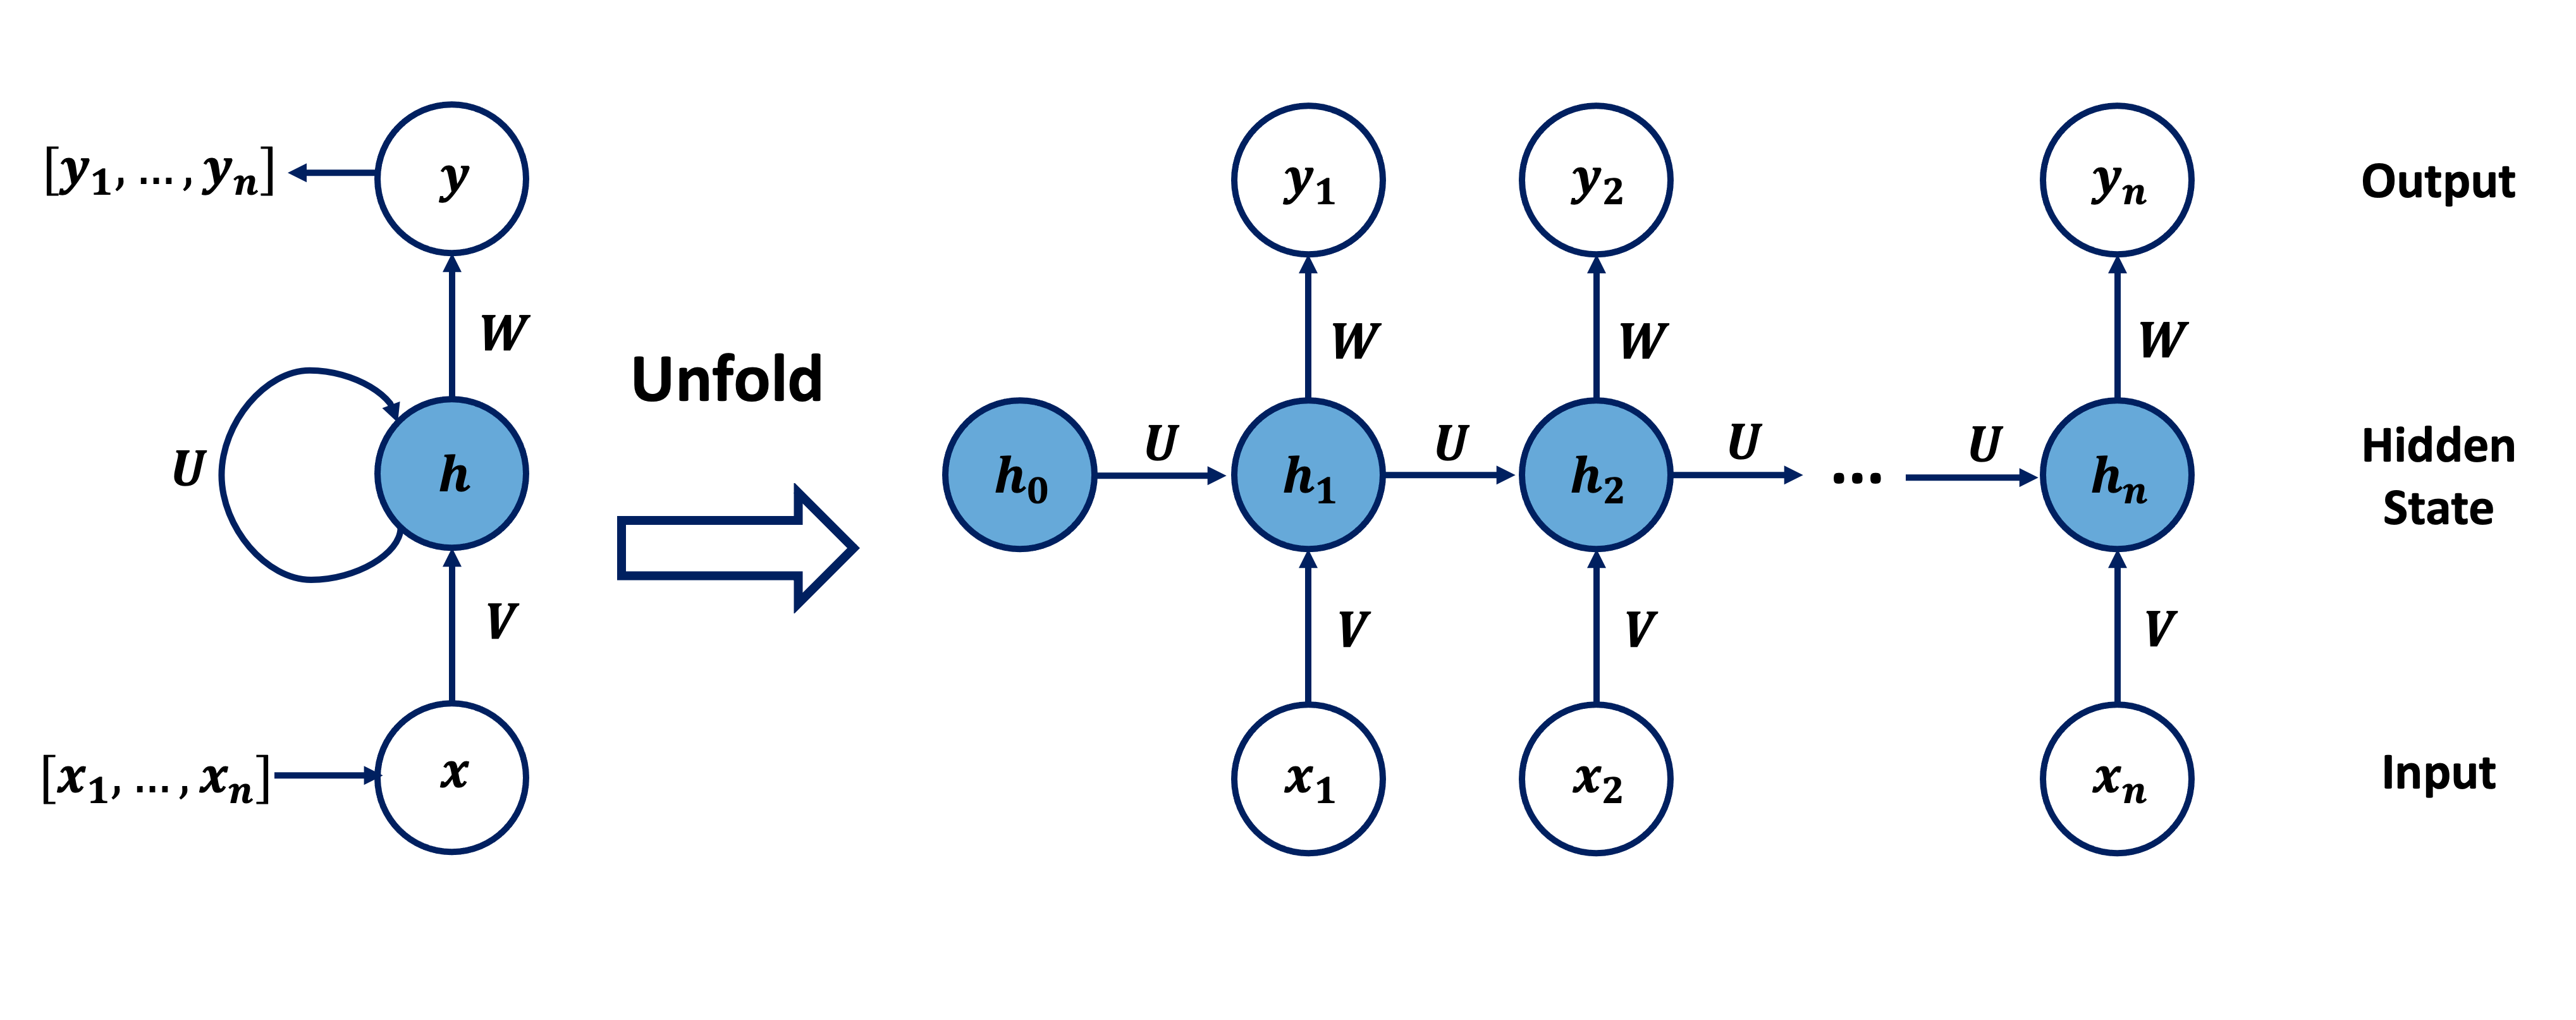
\includegraphics[scale=0.5]{Images/ML/rnn.png}
    \caption{A recurrent neural network, using 3 feed-forward neural networks (DNN) $U$, $V$, $W$, to map the input sequence $x = [x_1, x_2, ..., x_N]$ to the output $y = [y_1, y_2, ..., y_N]$ using the internal hidden state $h^t$ evovling for each timestep $t$. $h_0$ would typically be obtained by a mapping of the whole input sequence $x$. } 
    \label{fig:rnnNet}
\end{figure}

\subsubsection{Long-Short Term Memory} 
As shown in Figure \ref{fig:lstmCell}, Long-Short Term Memory (\gls{lstm}) cells implement a specific architecture to propagate information along the sequence, with the introducion of a new control state $c$ \cite{lstmPaper}. Three gates covering the forget, the input, and the output regulate the flow of information from the cell. In particular, the forget gate $F$ decides what information to keep from prior states, by multiplying these values by a factor 1 and discards the rest through a multiplication by a factor close to 0. The input gate $I$ is tasked with creating the new internal state of the cell and what information to store in it. Finally, the output gate $O$ decides what information in the cell should be brought to the output. This selectivty of the \gls{lstm} cell to decide what to use from memory, what to keep in memory, and what to output give this architecture a much improved memory for long sequences which result in a much improved efficiency. 

\begin{figure}[h!]
    \center
    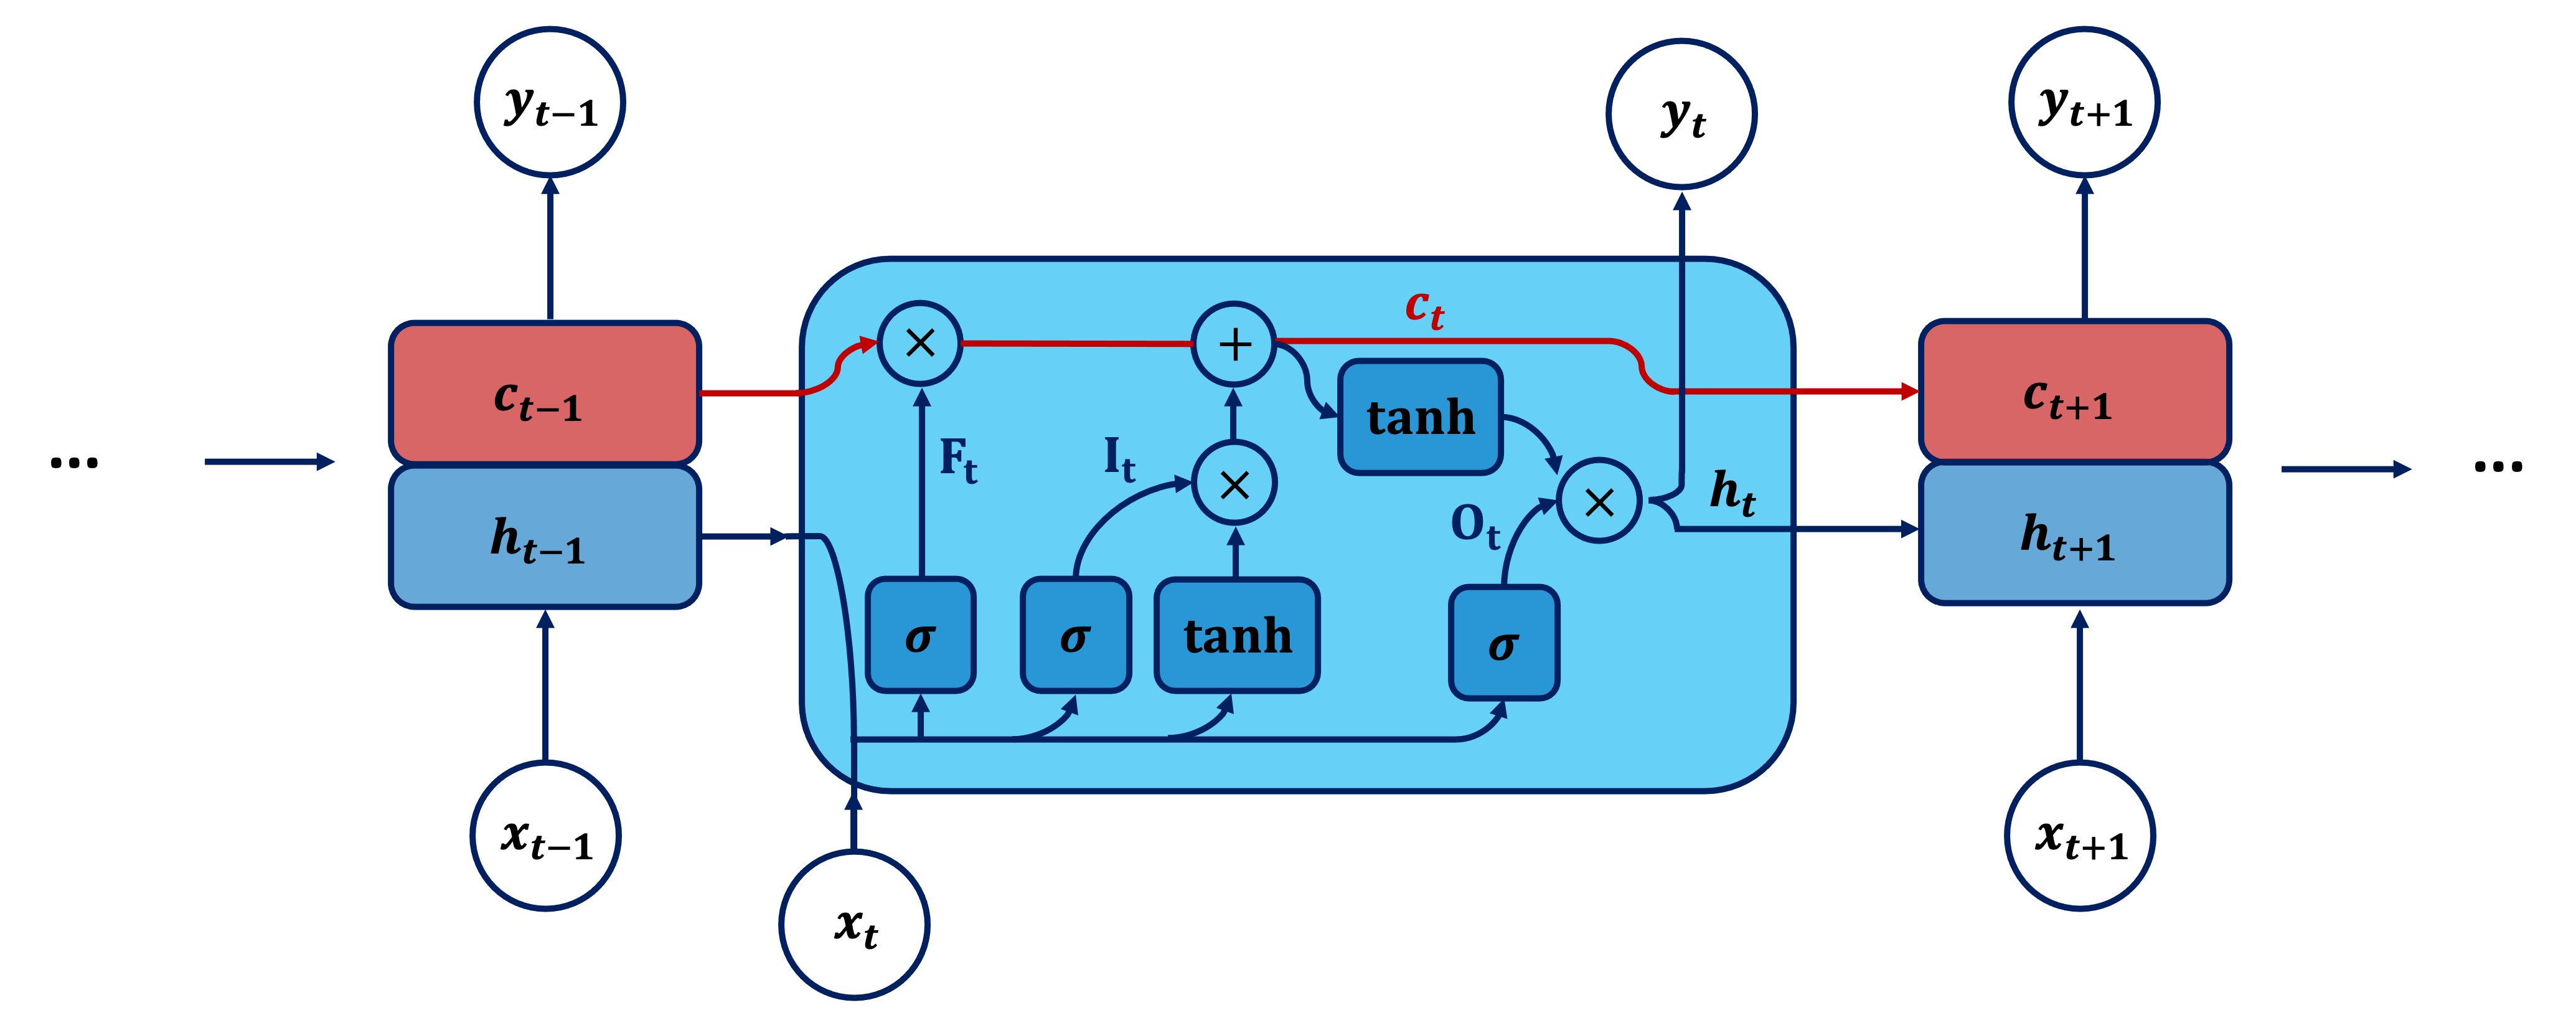
\includegraphics[scale=0.5]{Images/ML/lstm.png}
    \caption{An LSTM cell. Arrows and lines that merge imply concatenation of the inputs, the $\times$, $+$, and tanh are element-wise operation and the $\sigma$ are different layered transformations (1-layer feed-forward network). $F_t$ is the forget gate of the memory cell $c$, $I_t$ the input gate, and $O_t$ the output gate. } 
    \label{fig:lstmCell}
\end{figure}

\subsubsection{Gated Recurrent Unit} 
The Gated Recurrent Unit (\gls{gru}) is another adventageous design to improve the memory of a recurrent-like network without using as many parameters as an \gls{lstm} \cite{gruPaper}. There is no output gate and only one internal hidden state $h_t$ is required. This architecture comes in different version, with the fully gated version presented in Figure \ref{fig:gruCell}. It only requires two gates: the \textit{update gate} $Z$ and the \textit{reset gate} $R$. The former lets the model decide how much of the past information should be kept and the latter is used to forget past information.

\begin{figure}[h!]
    \center
    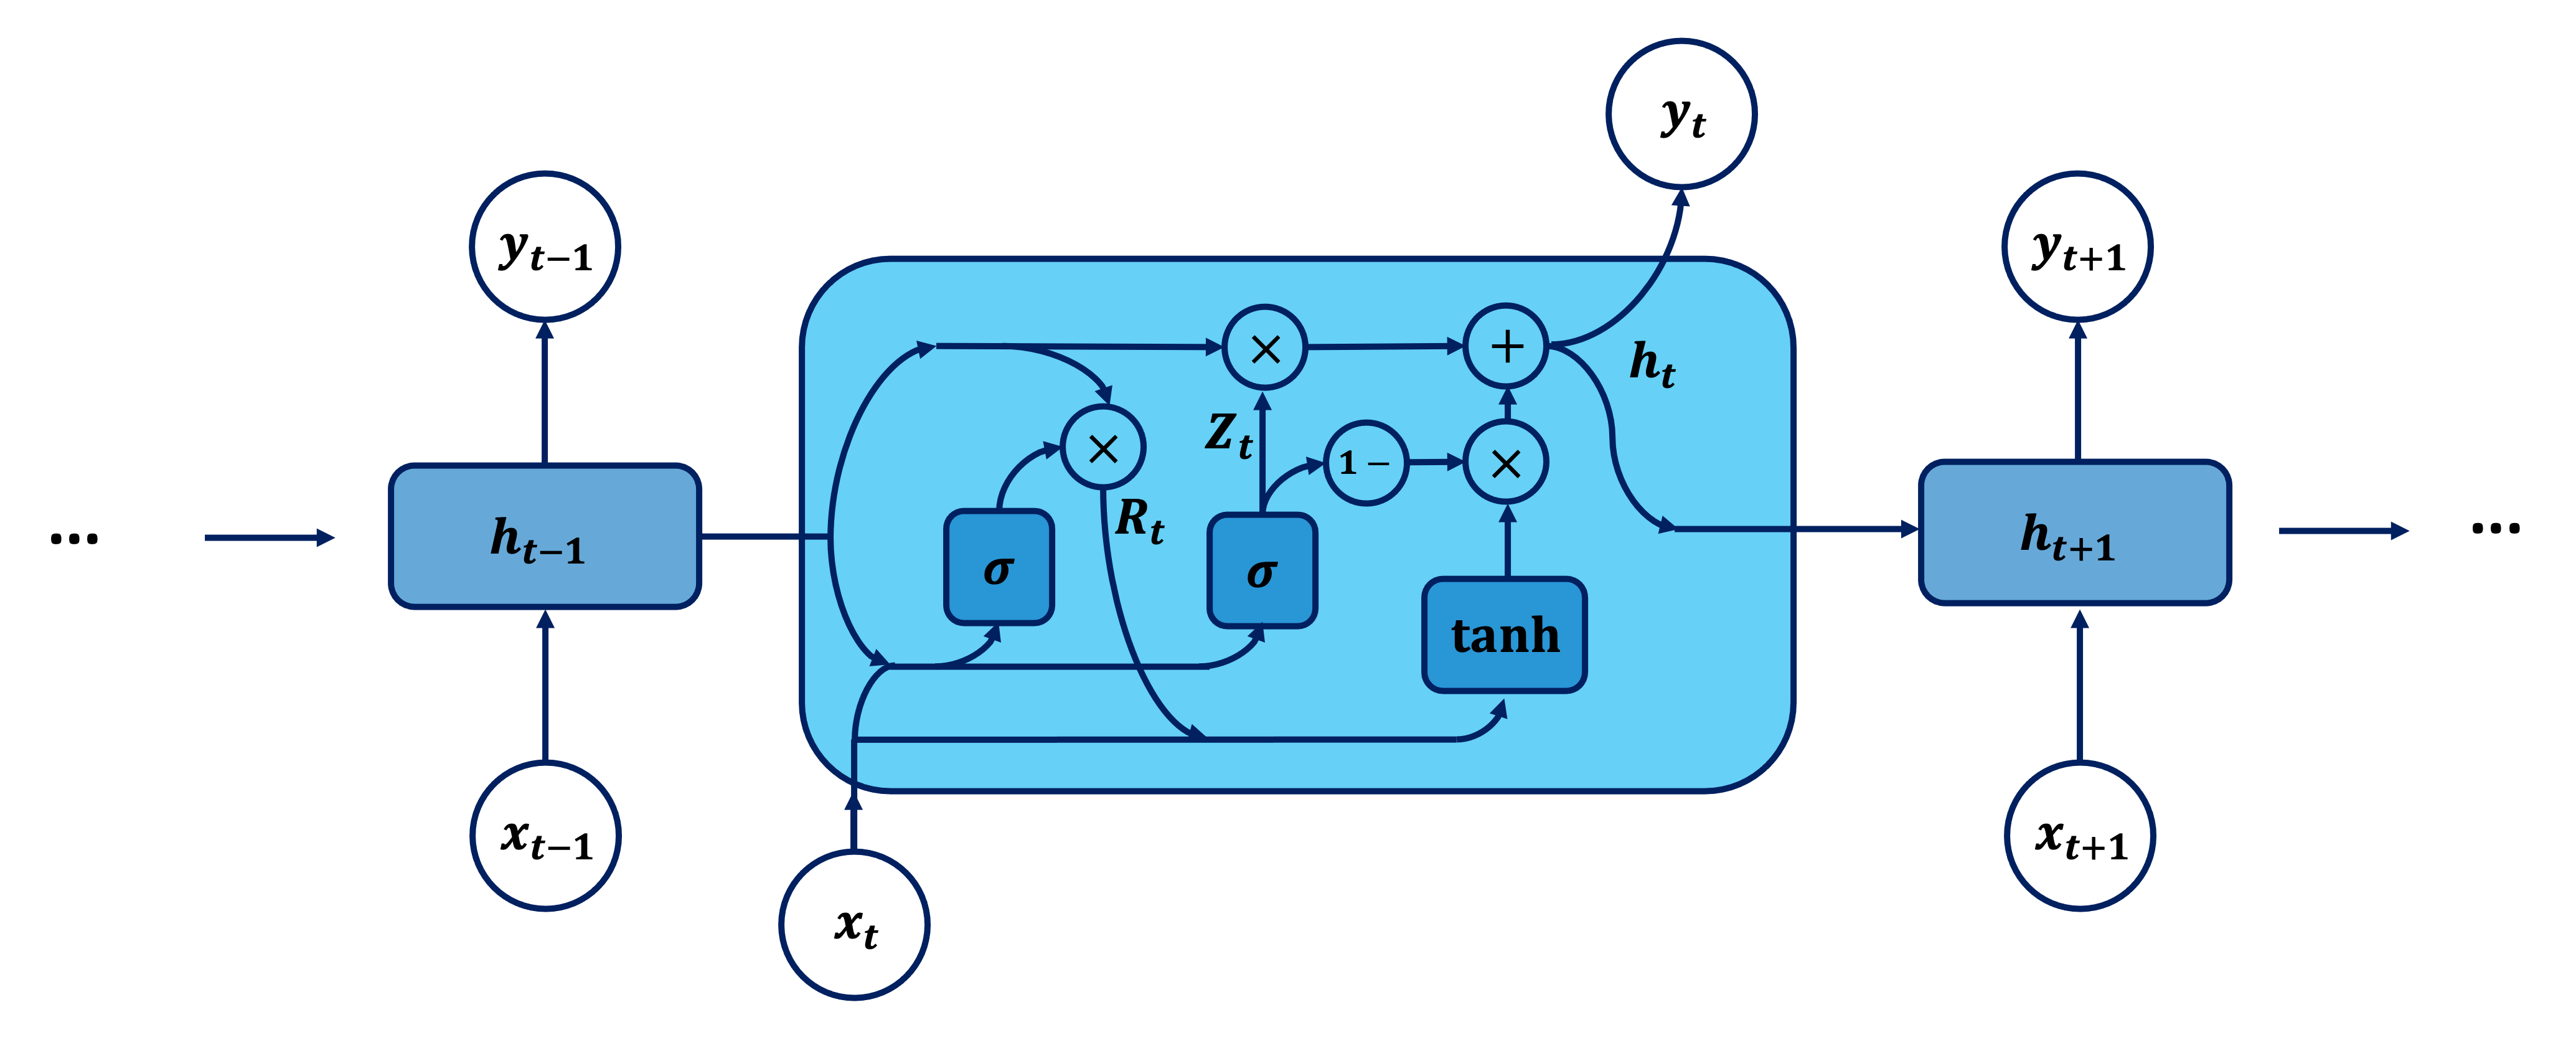
\includegraphics[scale=0.5]{Images/ML/gru.png}
    \caption{A Gated Recurrent Unit cell (fully-gated version). Arrows and lines that merge imply concatenation of the inputs, the $\times$, $+$, tanh, and ``1 - '' are element-wise operation - the last one outputting the vector 1 minus its inputs - and the $\sigma$ are two different layered transformations (1-layer feed-forward network) with sigmoid-like activation function. $Z_t$ is the update gate and $R_t$ the reset gate. } 
    \label{fig:gruCell}
\end{figure}

\gls{rnn}s and their modification have been designed for ordered sequence analysis and have had great results in such settings. Ordered sequences are natural in language analysis, where a sentence such as \textit{``the boy hit the car''} is meaninguflly different to its permutation \textit{``the car hit the boy''}. The choice to sequentially analyse the tokens of a sequence with memory lets \gls{rnn}-based operates simularly to a Turing Machine, endowing them with the powerful representational flexibility of Universal Turing Machine \cite{NEURIPS2021_ef452c63}. A significant drawback however is the impossibility to fully parallelise the analysis of the sequence due to its strict ordering, making \gls{rnn}s expensive models to train even on highly parallelised hardware. The main motivation behind the Transformer design, introduced in section \ref{sec:transformer}, was to fix this crucial weakness. \\

\paragraph{Pros:}
\begin{itemize}
    \item \textit{Sequential Processing:} \gls{rnn} are designed to handle sequential data, making them suitable for tasks with temporal dependencies.
    \item \textit{Flexibility:} \gls{rnn} can operate on input sequences of variable length.
    \item \textit{Memory:} \gls{rnn} have a memory mechanism that allows them to retain information about previous inputs.
\end{itemize}

\paragraph{Cons:}
\begin{itemize}
    \item \textit{Vanishing and Exploding Gradients:} Training deep \gls{rnn} can suffer from vanishing and exploding gradient problems, affecting the learning of long-term dependencies.
    \item \textit{Limited Short-Term Memory:} Traditional \gls{rnn} struggle to capture long-range dependencies due to their limited short-term memory. 
    \item \textit{Complexity:} While \gls{lstm} and \gls{gru} architectures can mitigate the two points above, the cost is a more complex architecture that is harder to train and requires more resources. 
    \item \textit{Interpretability:} The internal workings of a \gls{rnn} is challenging to interpret.
\end{itemize}

\subsection{Convolutional Neural Networks}
Convolutional Neural Networks (\gls{cnn}) \cite{NIPS198953c3bce6, NIPS2012_c399862d} have emerged as a powerful class of deep learning models that are particularly effective in computer vision tasks, including image and video analysis. The architecture of \gls{cnn}s is roughly based on human visual processing. It consists of convolutional layers - implementing the fundamental convolution operation-, pooling layers, and feed-forward layers (\gls{dnn}). This architecture, presented in Figure \ref{fig:cnnDesign}, enables \gls{cnn} to automatically learn hierarchical representations of features while respecting properties of image-based data: spaciality (geometrical grounding), locality (neighbourhoods) and spatial symmetry.

\begin{figure}[h!]
    \center
    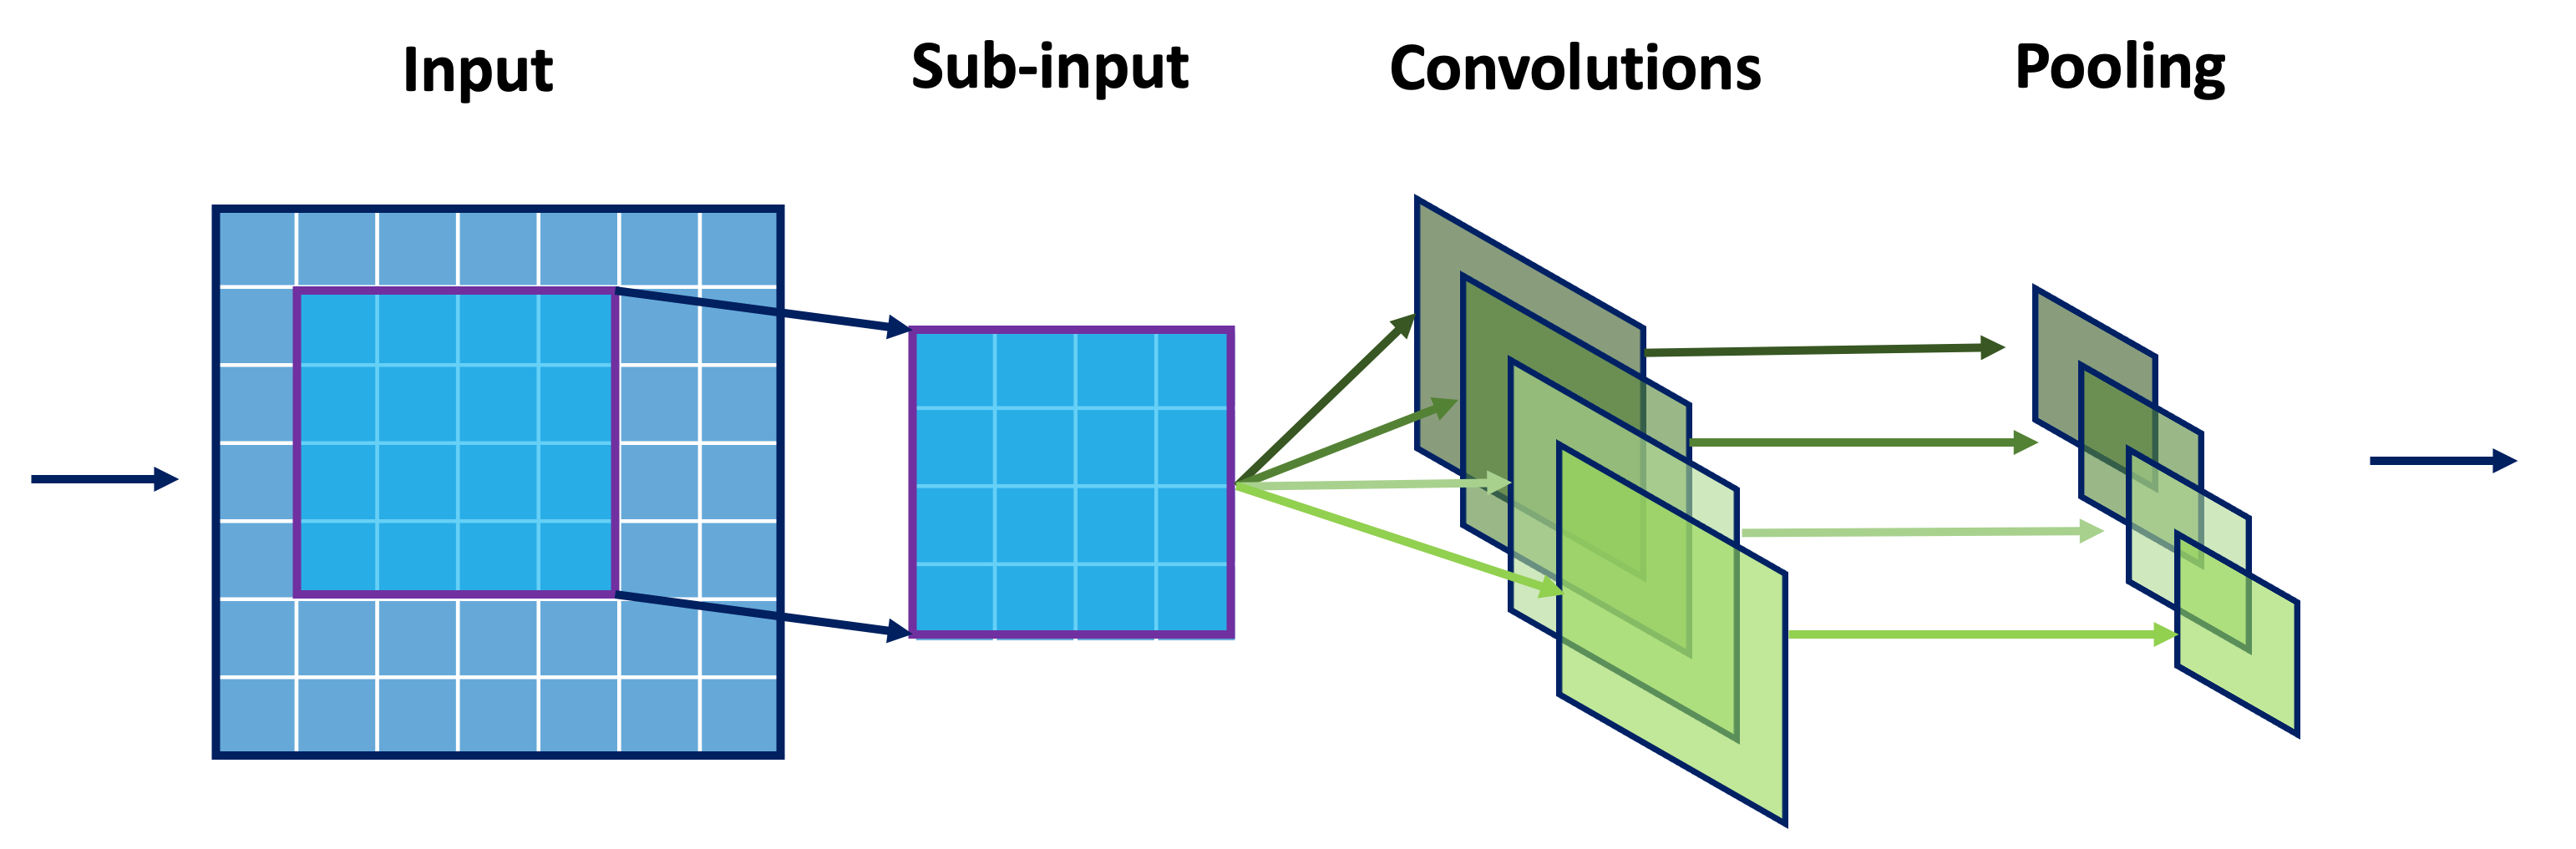
\includegraphics[scale=0.5]{Images/ML/cnn.png}
    \caption{A layer of a convolutional neural network, implementing a convolution with 4 kernels followed by a pooling operation. This design can be stacked to create deep architecture, and combined with a feed-forward neural network, after flattening the output at some depth, before reaching the final loss function layer. In this example, the receptive field size is 4 and there are 4 different kernels used to analyse an input image of size 7 $\times$ 7.} 
    \label{fig:cnnDesign}
\end{figure}

The functioning of \gls{cnn} involves the use of convolutional layers to extract local patterns and features from input data. Convolutional operations are applied to the input data by multiplying entry-by-entry a learnable \textit{kernel} or \textit{filter}, represented by a matrix of weights of smaller dimension than the total image size, with an equal size subpart of the input and applying an activation function. The size of the filter or kernel restricts the processing of the input to a given \textit{receptive field} dimension, and this window is passed over the full input image by moving it by a defined \textit{stride} length. Pooling layers are then used to reduce spatial dimensions and retain important features. This process can be parallelised for an image of multiple channel: e.g., a coloured image would be represented by a tuple of 3 values (for example, using the RGB coding) for each pixel. For classification and regression, a \gls{cnn} based model would typically stack several convolutional and pooling layers before leading to a fully connected neural network ``flattening'' the last representation to make predictions. \textit{Flattening} refers to the process of transforming the input image, represented as a matrix $\mathbb{R}^{x} \times \mathbb{R}^{y}$, into a vector $\mathbb{R}^{x \times y}$. \gls{cnn}-based models, such as AlexNet \cite{NIPS2012_c399862d} and ResNet \cite{resNetPaper}, have demonstrated state-of-the-art performance in various computer vision tasks.\\
A main advantage of the convolution operation on an image of size $x \times y$ is the reduction of the number of artificial neurons required to process the image, which helps to regularise the network.
\begin{itemize}
    \item A \gls{dnn} given the flattened image would require $x \times y$ neurons. 
    \item A \gls{cnn} with $k$ kernels of size $\alpha \times \beta$ would require $k \times \alpha \times \beta$ artificial neurons, that would be applied to different subpart of the image. 
\end{itemize}
For example, for an image of size 100 $\times$ 100, a \gls{dnn} would require 10,000 weights while a \gls{cnn} can process the image with only 25 if a single kernel of size 5 $\times$ 5 is used. Typical pooling functions are the \textit{maxPooling} or the \textit{sumPooling}, which, respectively, takes the largest element or the sum in each window of their input, with specific hyperparameters governing the size and the movements of the window.\\
\paragraph{Pros:}
\begin{itemize}
    \item \textit{Feature Learning:} \gls{cnn} automatically learn hierarchical representations of features on multidimensional data, reducing the need for manual feature engineering.
    \item \textit{Spatial Hierarchies:} Convolutional and pooling layers enable the model to capture spatial hierarchies in the input data while respecting the properties of images, namely locality: how close pixels are. 
    \item \textit{State-of-the-Art Performance:} \gls{cnn} have achieved state-of-the-art performance in image classification, object detection, and segmentation tasks.
\end{itemize}

\paragraph{Cons:}
\begin{itemize}
    \item \textit{Computational Complexity:} Training deep \gls{cnn} can be computationally intensive, requiring substantial resources.
    \item \textit{Large Datasets:} \gls{cnn} often require large labelled datasets for effective training, which may not be available for every application.
    \item \textit{Interpretability:} The internal workings of \gls{cnn} can be challenging to interpret, making them somewhat of a "black box".
\end{itemize}

\subsection{Graph Neural Networks}
In the last few years, \gls{gnn} have gained significant attention for their ability to model and analyse complex relationships within graph-structured data \cite{graphNetRef}. Originally designed for tasks such as node classification and link prediction, \gls{gnn}s have found applications in diverse domains such as social networks modelling, recommendation systems, and physics, for modelling the dynamic of a $N$-body system, performing tracks reconstruction, and identifying particles.\\
\gls{gnn}s operate on graph-structured data, where nodes or vertices represent entities, and edges represent relationships between these entities. The functioning of \gls{gnn}s involves iterative aggregation of information from neighbouring nodes and updating of the edges, allowing them to capture local and global structures as defined by the graph. This is achieved through the use of message-passing mechanisms. An interesting feature of graphs is that the input information does not need to be given a rigid structure. Consequently, graph based-methods have a much greater representation power than image- or sequence-based ones. Graphs are in fact able to represent abritrary relational structures, as defined by the graph through its directional weighted edges \cite{graphInductiveBias}. A particular feature arising from this property is that graph are permutation equivariant: the order of nodes can be rearranged without impact. \\

\begin{figure}[h!]
    \center
    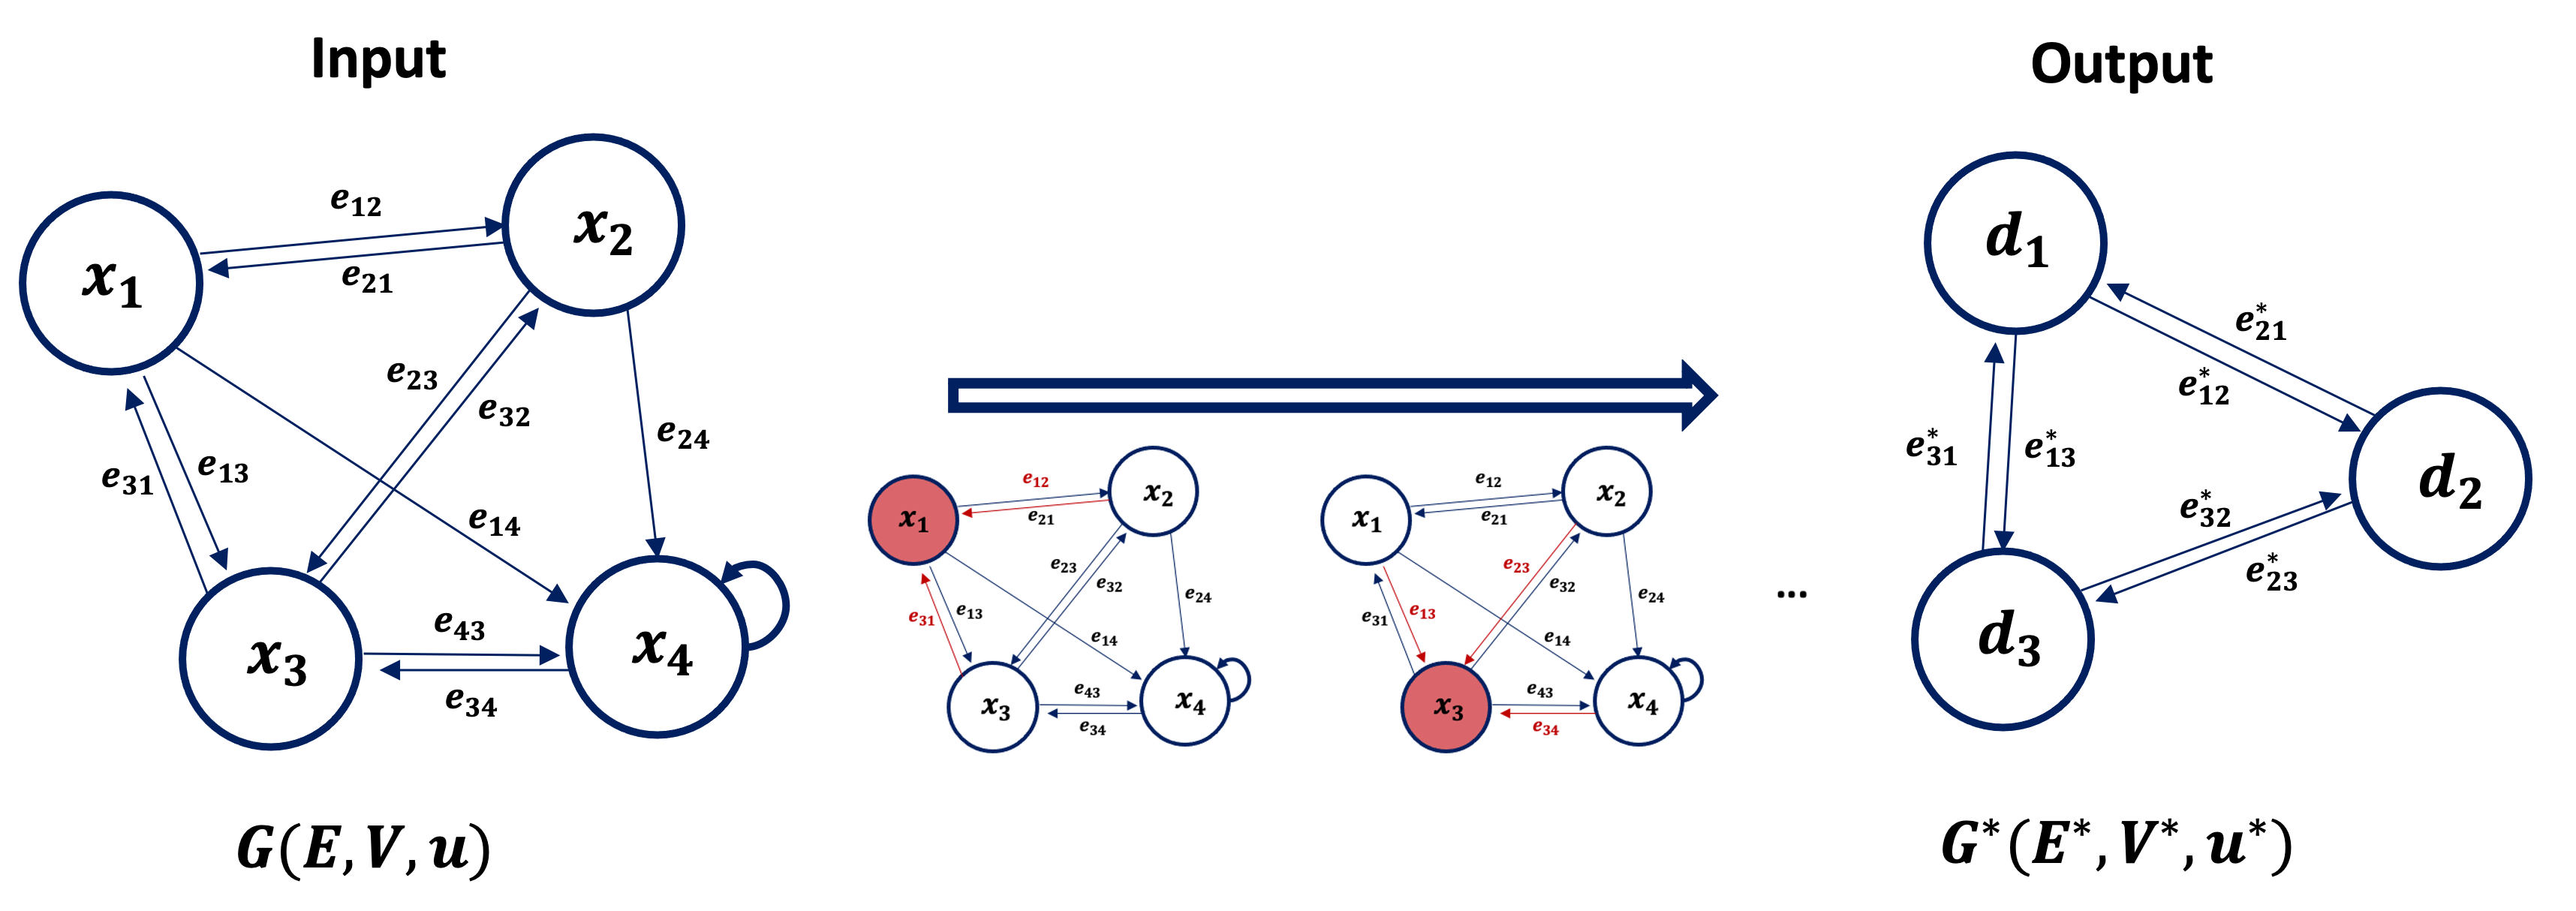
\includegraphics[scale=0.5]{Images/ML/gnn.png}
    \caption{A graph neural network update on a directed graph $G(V, E, u)$ with a global representation $u$, four initial nodes $\in V$ and edges $e_{ij} \in E$ connecting nodes $i \rightarrow j$ (in the notation of the text, each node is given a different integer index $k$ and written $(e_k, r_k, s_k)$, with $r_k = j$ and $s_k = i$). By analysing the neighbours of each node, the graph is updated to a new graph $G^*(V^*, E^*, u^*)$.} 
    \label{fig:gnnScheme}
\end{figure}

Typically, a \gls{gnn} architecture consists of multiple layers of message passing operations. Each layer updates the node representations by aggregating information from neighbouring nodes, as schematised in Figure \ref{fig:gnnScheme}. Different architectures implement different update processes for the graph, with popular \gls{gnn} architectures being Graph Convolutional Networks (GCNs) \cite{gcnPaper} and Graph Attention Network \cite{velickovic2018graph}. In this thesis, the notation adopted is to represent a graph $G$ has a tuple of three entires:
\begin{enumerate}
    \item $E = \{(e_k, r_k, s_k)\}_{k=1:N^e}$ the set of edges, with each edge having a real vector of features $e_k \in \mathbb{R}^e$ and storing the index of the receiver (sender) as $r_k$ ($s_k$).
    \item $V = \{v\}_{i=1:N^v}$ the set of nodes, each node having a real vector of features $v_i \in \mathbb{R}^v$.
    \item $u$, a global attribute of the graph modelled by a real vector of features $u \in \mathbb{R}^u$. 
\end{enumerate}

\begin{algorithm}
    \caption{Steps of Computation in a Full Graph Network Block \cite{graphInductiveBias}}
    \label{algo:graph_network}
    \begin{algorithmic}[1]
    \Function{GraphNetworkUpdate}{$E, V, u$}
        \For{$k \in \{1 \ldots N^e\}$}
            \State $e^*_k \gets \phi^e(e_k, v_{r_k}, v_{s_k}, u)$
        \EndFor

        \For{$i \in \{1 \ldots N^n\}$}
            \State Let $E_i^* = \{(e^*_k, r_k, s_k)\}$ for $k = 1 : N^e$ where $r_k = i$
            \State $\overline{e^*_i} \gets \rho^{e \to v}(E^*_i)$
            \State $v^*_i \gets \phi^v(\overline{e^*_i}, v_i, u)$
        \EndFor

        \State Let $V^* = \{v^*\}_{i=1}^{N^v}$
        \State Let $E^* = \{(e^*_k, r_k, s_k)\}_{k=1}^{N^e}$
        \State $\overline{e^*} \gets \rho_{e \to u}(E^*)$
        \State $\overline{v^*} \gets \rho_{v \to u}(V^*)$
        \State $u^* \gets \phi_u(\overline{e^*}, \overline{v^*}, u)$

        \State \Return $(E^*, V^*, u^*)$
    \EndFunction
    \end{algorithmic}
\end{algorithm}

The most general graph update algorithm to describe an update stage of a full \gls{gnn} block is described in Algorithm \ref{algo:graph_network}. Essentially, for a given step the input is a graph $G(E, V, u)$ that is updated into a new graph $G^*(E^*, V^*, u^*)$ by first updating the edges $e \in E$ and then modifying the nodes $v \in V$ and the global representation $u$. The update rule leverages different neural networks $\phi$ and aggregation function $\rho$ to update the graph. The aggregation function should accept a variable number of input with permutation invariance to output a single element per group, and is typically implemented to do the sum or max pooling. The update is decomposed into successive updates of: 
\begin{itemize}
    \item The edges, with a \gls{dnn} $\phi^e$ mapping each of the input edge, their respective receiver and sender nodes and the global state $u$ to output a new edge feature vector $e^*_k$ for each edge $k$: $e^*_k = \phi^e(e_k, v_{r_k}, v_{s_k}, u)$. The new edges are stored in a set $E^*$. 
    \item Before updating a vertex $i$ represented by $v_i$, the $E_i^*$ updated edges connecting to $i$ ($i == r_k$) are pooled locally over the node as $\overline{e^*_i} = \rho^{e \rightarrow v}(E_i^*)$.
    \item The vertex is then updated with a \gls{dnn} $\phi^v$, mapping the pooled representation of the edges $\overline{e^*_i}$ connecting to the vertex being updated, the input vertex feature $v_i$ and the global representation $u$ to update $v_i \rightarrow v^*_i = \phi^v(\overline{e^*_i}, v_i, u)$. The new vertices are stored in a set $V^*$.
    \item The set of edges is updated by a global pooling $\overline{E^*} = \rho^{e \rightarrow u}(E^*)$.
    \item The set of vertices is updated by a global pooling $\overline{V^*} = \rho^{v \rightarrow u}(V^*)$.
    \item The global representation is updated by \gls{dnn} $\phi^u$ mapping $u^* = \phi^u(\overline{e^*}, \overline{v^*}, u)$, where $\overline{e^*} = \rho^{e \rightarrow u}(E^*)$ and $\overline{v^*} = \rho^{v \rightarrow u}(V^*)$ are globalyl pooled updated edges ($\overline{E^*}$) and vertices ($\overline{V^*}$). 
\end{itemize} 
This formulation of a graph as a message-passing with edges update device is the most complete architecture of a \gls{gnn}. The design is however flexible: for example, \gls{rnn}s or \gls{cnn}s can be used instead of \gls{dnn}. Furthemore, many specialisations of the structures exist to reduce the degree of complexity of the model and avoid overfitting or converge issues, as listed in Figure \ref{fig:diverseGNN}. A notable example for this thesis is the Deep Set architecture \cite{NIPS2017f22e4747}, designed to runs specifically on sets where the ordering does not matter. It essentially simplifies the graph network by dropping altogether the edges and considering instead a fully connected graph with static edges, with an update of the global representation only based on pooled node information: 
\[v^*_i = \phi^v(\overline{e^*_i}, v_i, u) = \phi^v(v_i, u),\] 
\[\overline{V^*} = \rho^{v \rightarrow u} = \sum_i v^*_i,\] 
\[u^* = \phi^u(\overline{e^*}, \overline{v^*}, u) = \phi^u( \overline{v^*}, u).\] This is somewhat simular to PointNet, a \gls{gnn} designed to analyse sets of 3D points, that uses an analoguous update with max-aggregation instead of sum pooling after updating the nodes in two steps \cite{pointNet}.  

\begin{figure}[h!]
    \centering
    \begin{subfigure}[b]{0.49\textwidth}
        \centering
        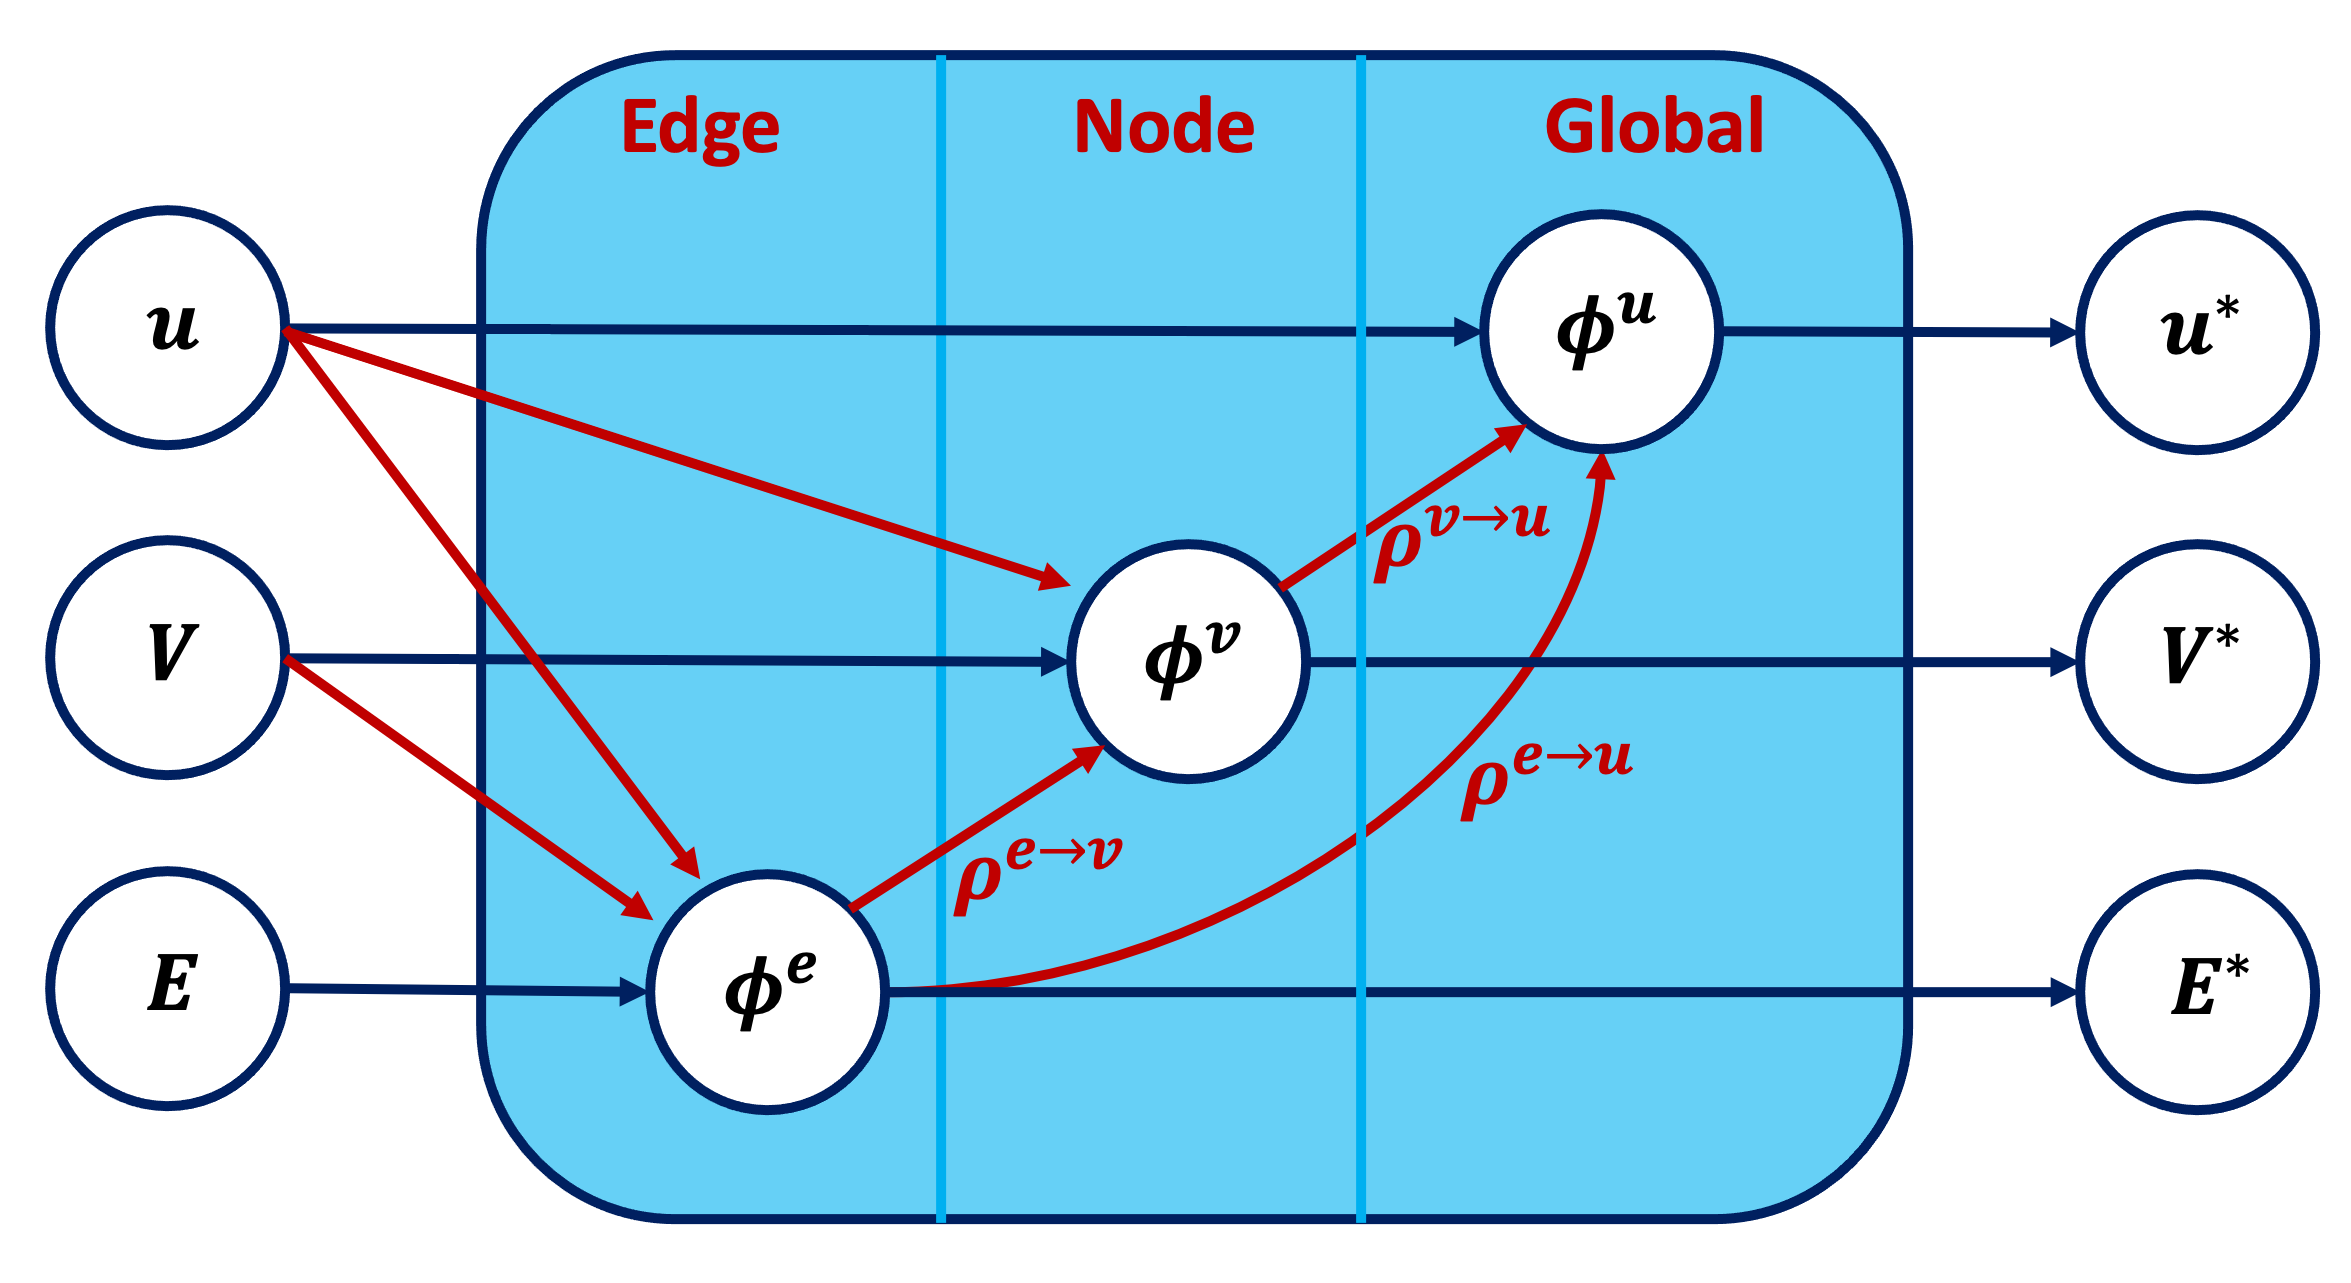
\includegraphics[scale=0.43]{Images/ML/fullGNN.png}
        \caption{Full \gls{gnn}.} 
        \label{fig:diverseGNNfull}
    \end{subfigure}
    \hfill
    \begin{subfigure}[b]{0.49\textwidth}
        \centering
        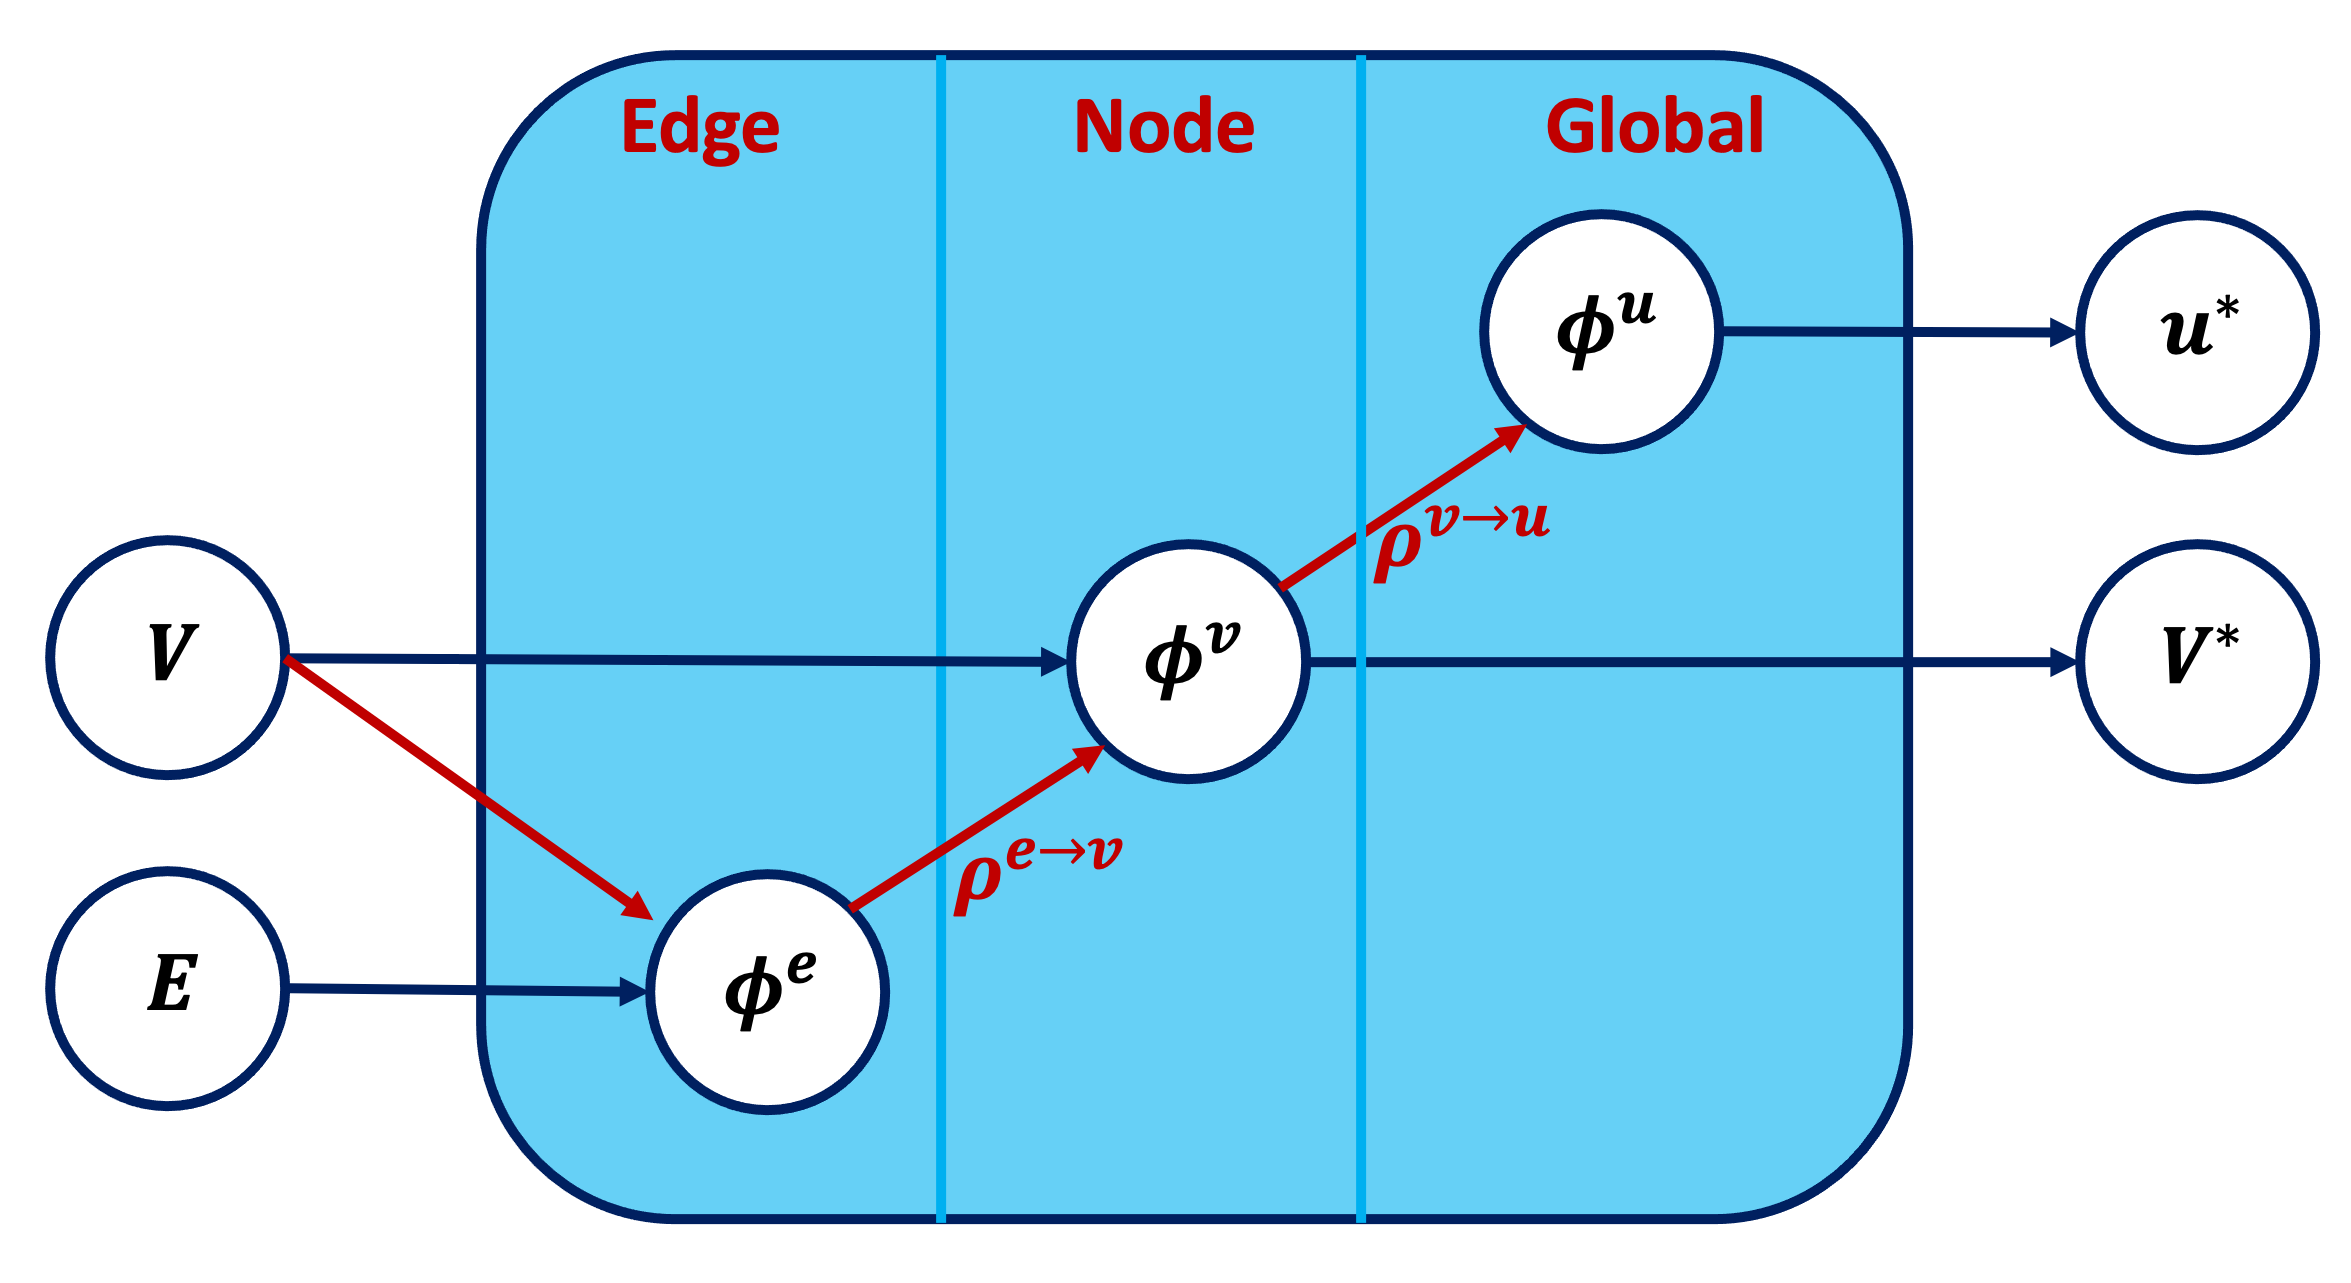
\includegraphics[scale=0.43]{Images/ML/messagepassingNN.png}
        \caption{Message-passing \gls{gnn}.} 
        \label{fig:pullsFTAGmp}
    \end{subfigure}
    \\  % newline
    \begin{subfigure}[b]{0.49\textwidth}
        \centering
        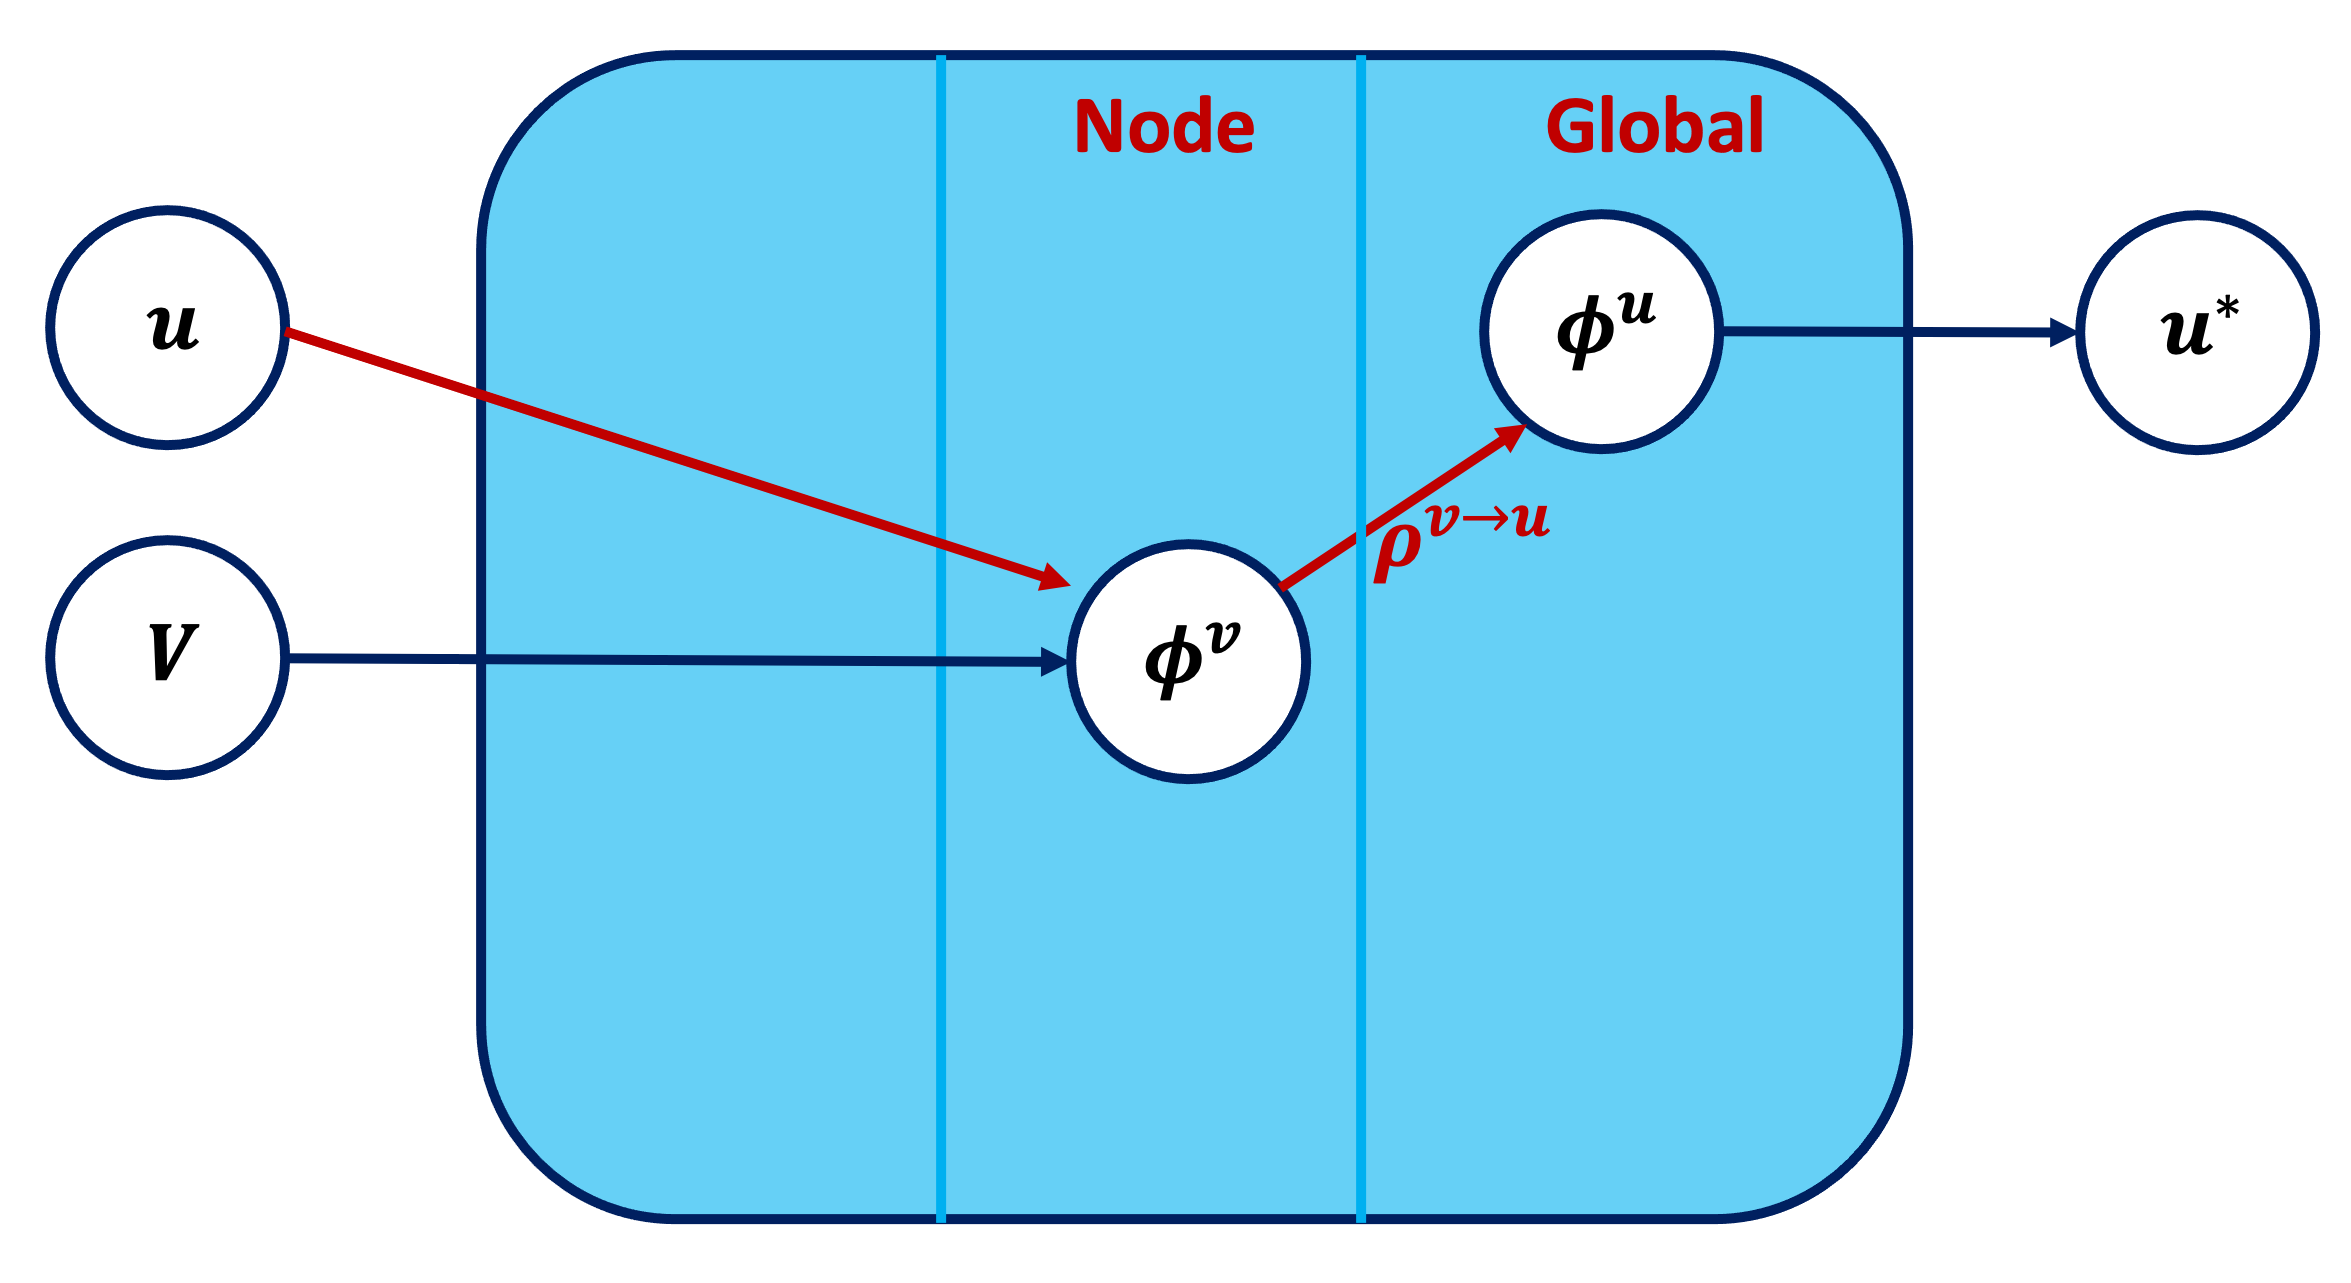
\includegraphics[scale=0.43]{Images/ML/deepSet.png}
        \caption{Deep Set.} 
        \label{fig:deepSetFig}
    \end{subfigure}
    \hfill
    \begin{subfigure}[b]{0.49\textwidth}
        \centering
        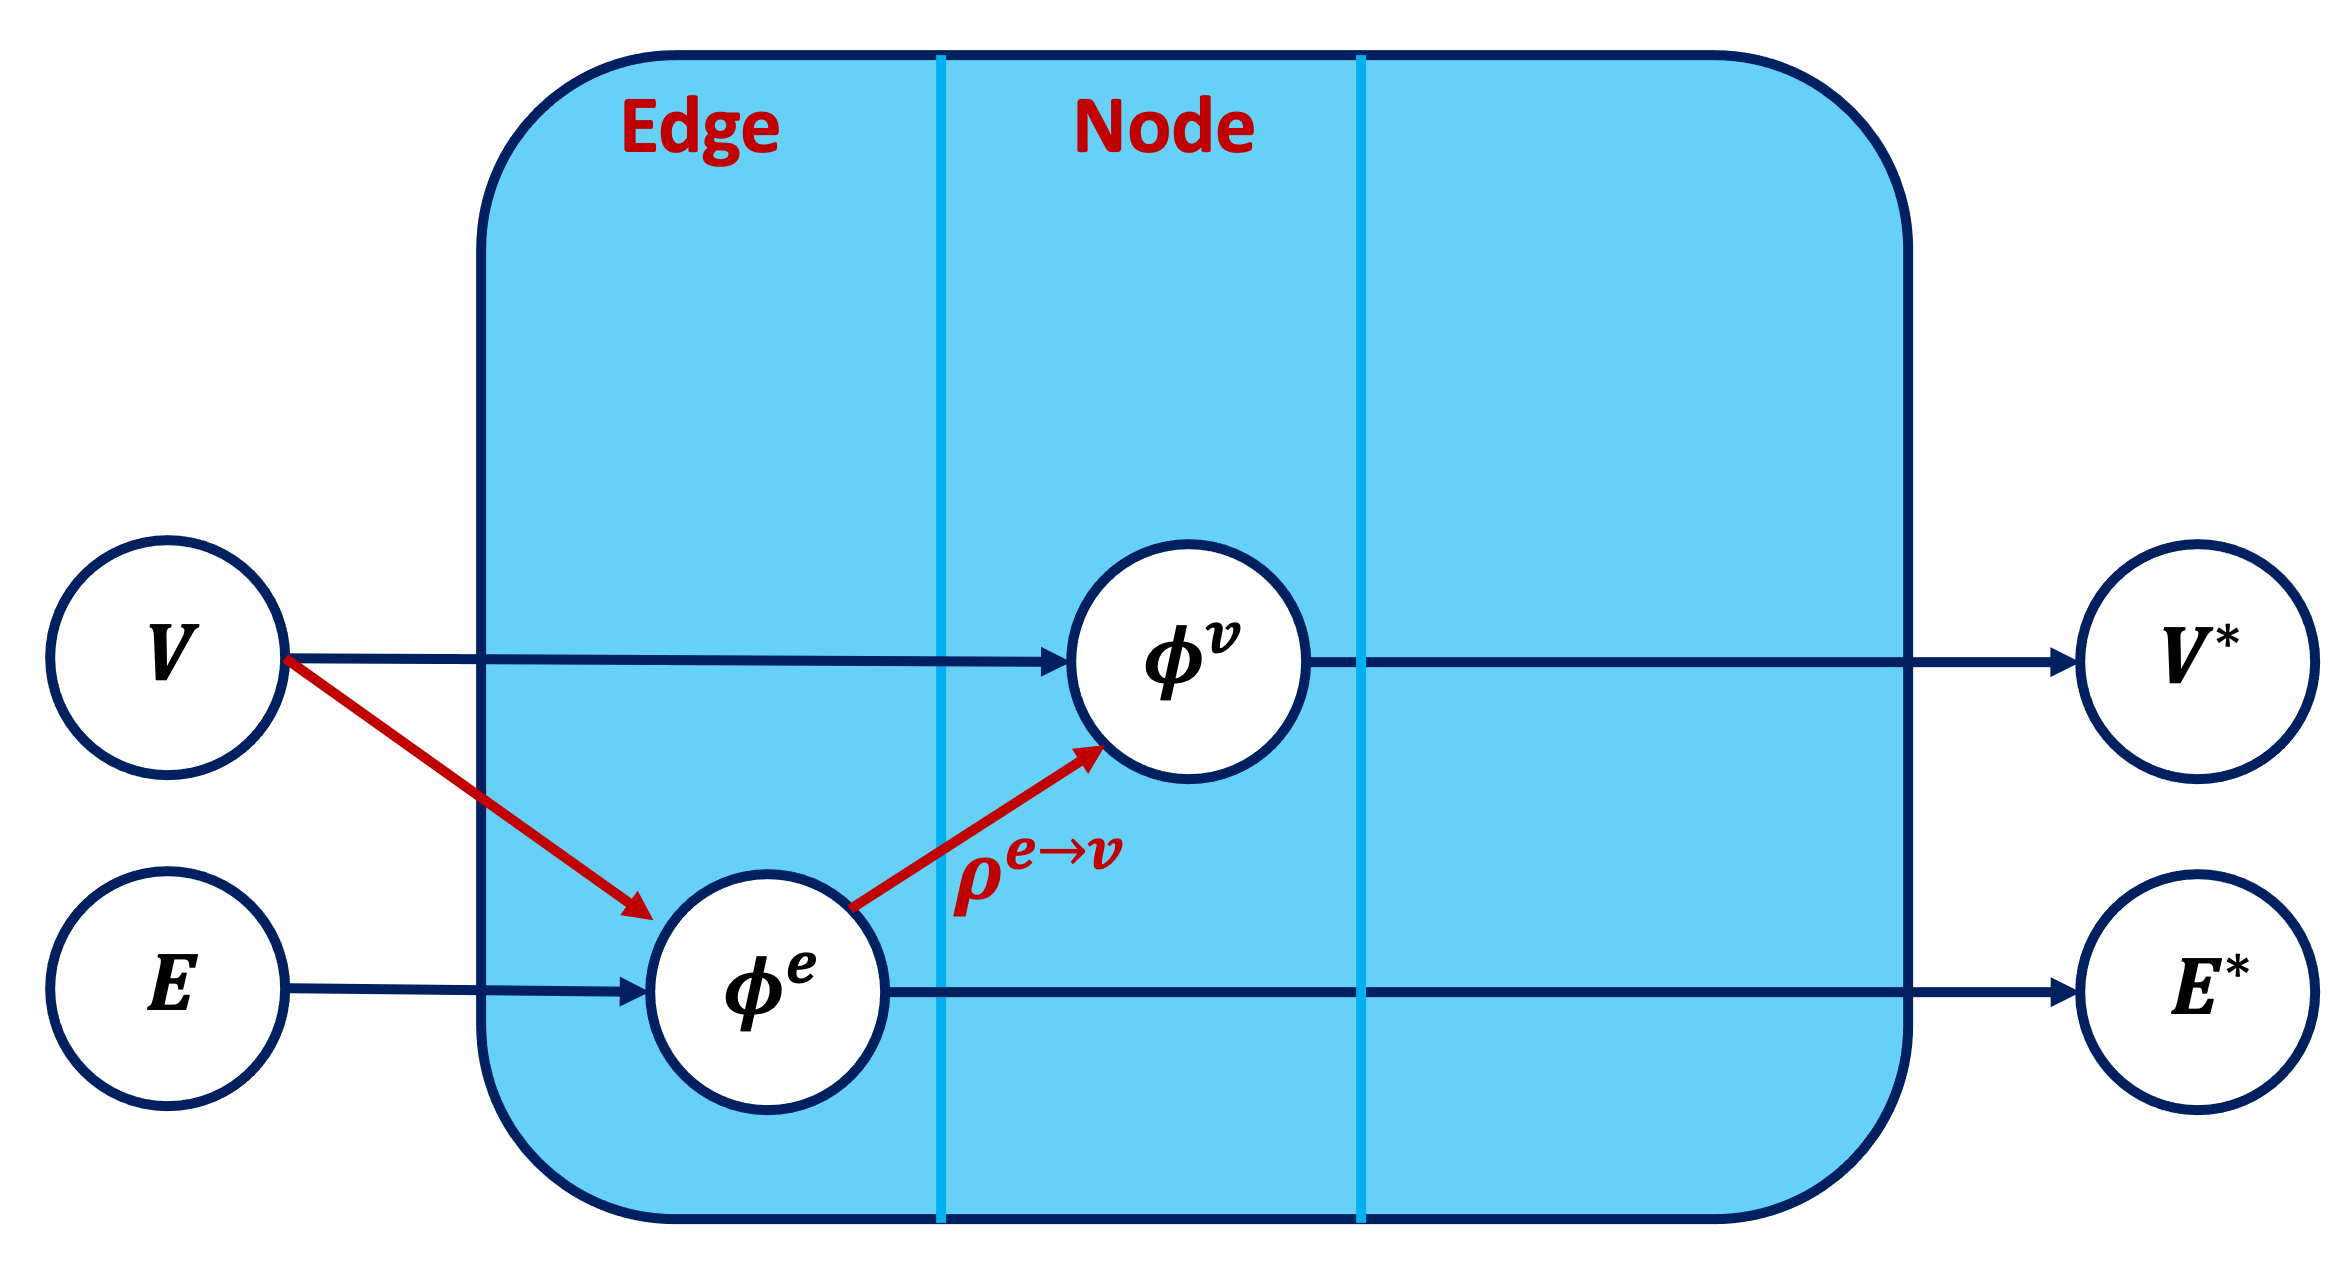
\includegraphics[scale=0.43]{Images/ML/nlnn.png}
        \caption{Non-local \gls{nn}.} 
        \label{fig:pullsFTAGnlnn}
    \end{subfigure}
    \caption{Different types of \gls{gnn} update rules, defining different \gls{gnn} architecture \cite{graphInductiveBias}.}
    \label{fig:diverseGNN}
\end{figure} 

A different approach introduced in \cite{nlnnPaper} defines the non-local neural network, unifying different types of \textit{attention}-based architecture. Attention is an essential feature of modern deep learning: it refers to how an element is given a weighted version of the inputs, with weights standing for the degree of attention to be given to each different part of the input. This concept is not restricted to \gls{gnn} but is easily encapsulated in this formalism. As will be shown in the next section, the Transformer is a special case of this non-local \gls{nn} family. In this section only the \gls{gat} is introduced for the sake of conciseness \cite{velickovic2018graph}. \gls{gat} introduces the attention mechanism by having a learnable weighting of the neighbour of the node being updated. When updating node $v_i$, a score is computed for each of the connected neigbour of $v_i$ by a \gls{nn} mapping: \[e(v_i, v_j) = \phi(v_i, v_j) = a^T \text{ leakyReLU}([W v_i, Wv_j]),\] where leakyReLU is the modification of the \gls{relu} with negative leakage, the nodes $v_i, v_j \in \mathbb{R}^d$ with $j$ connected to $i$, and the operation implements an embedding of the two nodes to a dimension $d'$ with two learnable parameters: $a \in \mathbb{R}^{2d'}$ and $W \in \mathbb{R}^{d' \times d}$. The operation $[,]$ stands for concatenation of the elements. These scores are then combined for each node $i$ over its neighbours $\{j\}$ to give attention scores $\alpha_{ij}$: \[ \alpha_{ij} = \text{softmax}_j (e(v_i, v_j)) = \frac{\exp(e(v_i, v_j))}{\sum_{j' \in \text{neighours of i}}e(v_i, v_{j'})}.\] The final step is to leverage these attention weights when updating each node $v_i$: \[v^*_i = \sigma\left(\sum_{j} \alpha_{ij} . W^v v_j \right),\] where the sum over $j$ is taken over neighbouring nodes of $i$, $\sigma$ is any activation function and $W^v$ is another matrix of learnable parameters.\\

\paragraph{Pros:}
\begin{itemize}
    \item \textit{Modeling Graph Structure:} \gls{gnn}s naturally handle graph-structured data, making them well-suited for tasks involving relationships between entities.
    \item \textit{Transferability:} Pre-trained \gls{gnn} models on one graph can be fine-tuned for related tasks on another graph.
    \item \textit{State-of-the-Art Performance:} \gls{gnn}s have achieved state-of-the-art results in various graph-related tasks, including node classification and link prediction.
\end{itemize}

\paragraph{Cons:}
\begin{itemize}
    \item \textit{Computational Complexity:} Training \gls{gnn}s can be computationally expensive, particularly for large graphs.
    \item \textit{Limited Global Context:} Some \gls{gnn} architectures may struggle to capture long-range dependencies in graphs, limiting their ability to consider global context.
    \item \textit{Interpretability:} Similar to other deep learning models, \gls{gnn} lack interpretability, making it challenging to understand the learned representations.
\end{itemize}

\subsection{The rise of the Transformers}\label{sec:transformer}

The Transformer architecture, introduced in 2017 \cite{NIPS_transformerPaper}, has become a foundational design for \gls{nlp} tasks. It has significantly impacted the field, enabling the development of state-of-the-art models such as BERT \cite{devlin-etal-2019-bert} and GPT \cite{radford2018improving}. More recentely, the transformer is also spearheading a revolution in computer vision tasks thanks to the generalisation of the architecture into the Vision Transformer (ViT) \cite{vitPaper}.

The Transformer architecture is based on the mechanism of self-attention introduced in the last section on graphs. As mentionned in section \ref{sec:RNN} on \gls{rnn}, it moves away from sequential processing and adopts a fully parallelised approach, allowing for efficient computation on dedicated hardware. The key components of the Transformer are the self-attention mechanism and position-wise feedforward networks. Self-attention allows the model to weigh the importance of different words or tokens in a sequence when assessing a specific token. This mechanism enables the model to capture long-range dependencies in the input data without the added complexity of \gls{lstm} or \gls{gru}. Strictly speaking, the input of a Transformer is a sequence that has no strict order. For \gls{nlp}, the important ordering of the sequence is built in the model using position-wise embedding. This lets the network decypher the index of the token in the input sequence and leverage this information for its tasks. For the computer vision case, the Vision Transformer first splits the input image $x$ into patches of fixed size, flattens them into a vector and maps them with a learnable positional embedding before processing them as a regular Transformer would.

\begin{figure}[h!]
    \center
    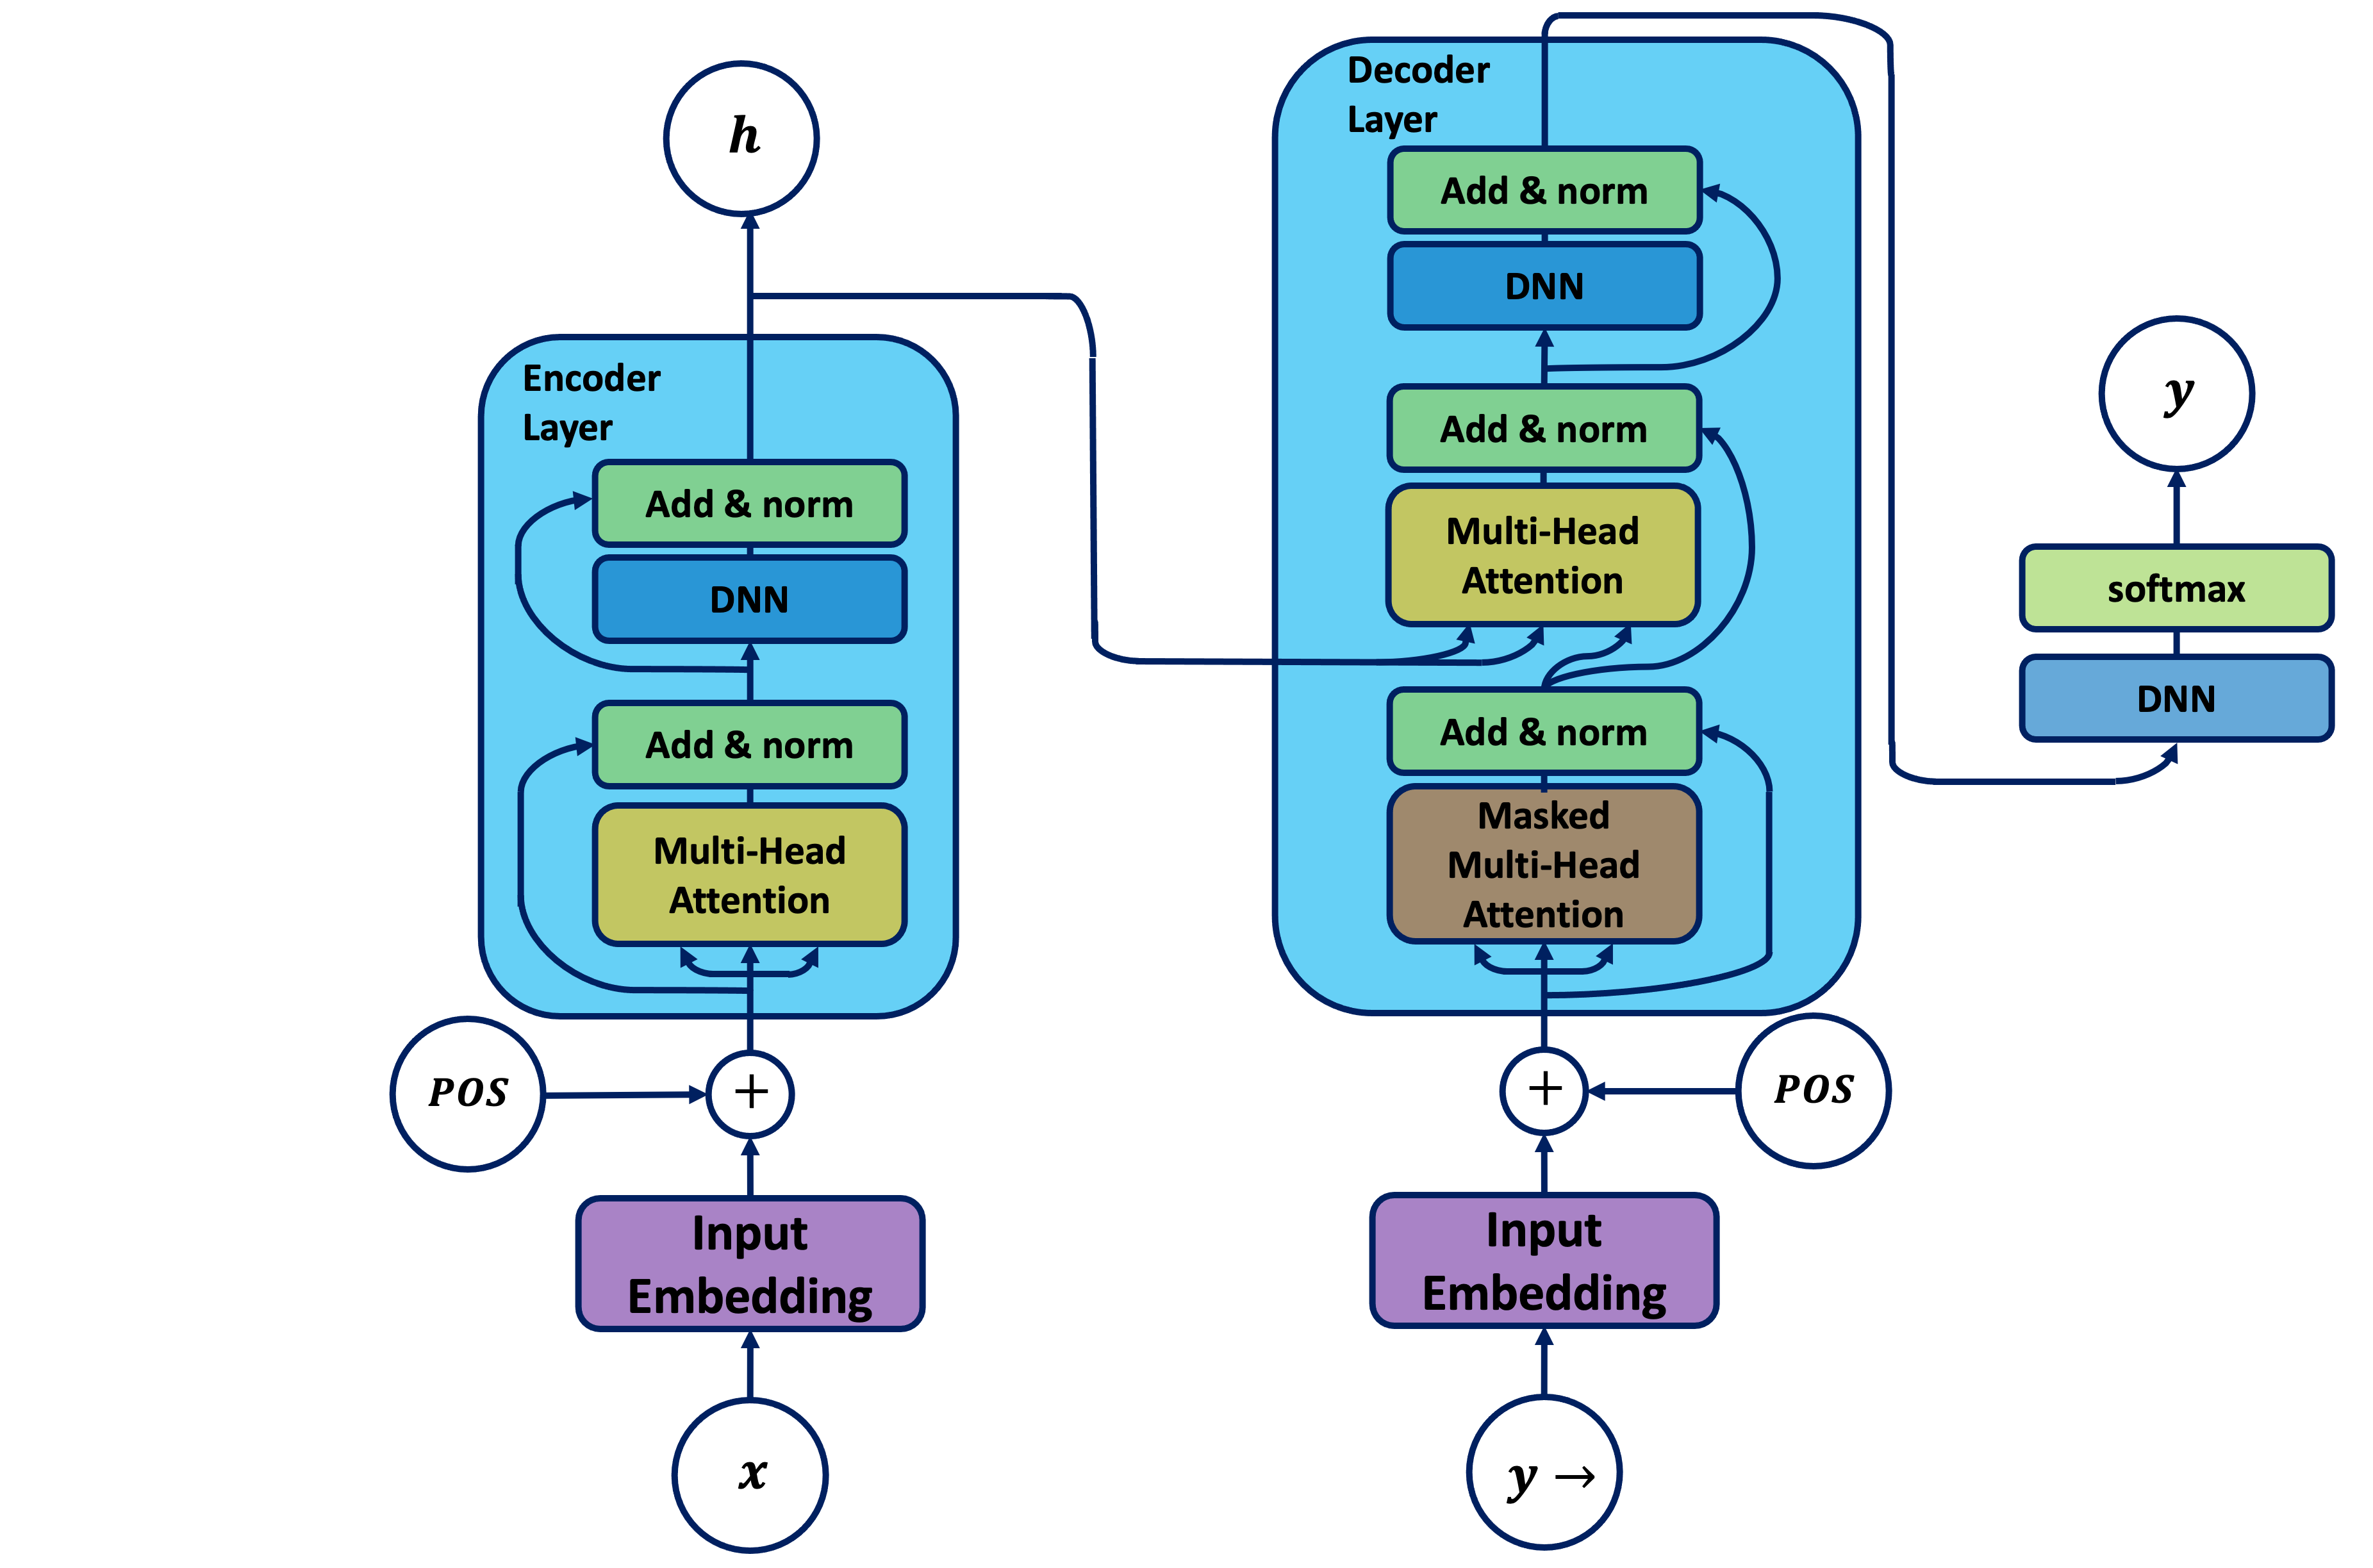
\includegraphics[scale=0.5]{Images/ML/transformer.png}
    \caption{The full transformer architecture, combining an encoder and a decoder each made of an arbitrary number of layers. The input $x$ is first embedded with a dedicated mapping which can, when order matters, be supplemented with positional embedding. The encoder generates an internal representation $h$ that is passed to the decoder. This component, depicted on the right, produces the next output using the internal representation $y$ and the output shifted to the right - to force output token to only access prior information. } 
    \label{fig:tranfoArchi}
\end{figure}

As presented in Figure \ref{fig:tranfoArchi}, the general Transformer architecture consists of an encoder and a decoder, the main feature of auto-encoder models. The decoder works in an autoregressive way, combining the current outputs $y_{t<T}$ with an internal representation $h$ built by the encoder to generate the next output tokens $y_{T}$. Both the encoder and the decoder are composed of multiple layers, each containing a multi-head self-attention mechanism and position-wise feedforward networks (\gls{dnn}). The decoder is further endowed with a masked attention layer, for the output to compute self-attention with information accessible prior to the token's position. The attention mechanism allows the model to focus on different parts of the input sequence, while the feedforward networks provide additional non-linear transformations. Residual connexions are added to let the gradients propagate efficiently in depth and layer normalisation is used after each block to avoid vanishing or exploding gradients and improve training speed \cite{ba2016layer}. This type of normalisation scales each activation (each neuron) by substracting the empirical mean and dividing by the standard deviation per datapoint. \\
The attention mechanism maps the queries and a set of key-value pairs to an output as defined in Equation \ref{eq:scdotatt} and schematised in Figure \ref{fig:scaledDotAtt}, with query $Q \in \mathbb{R}^{d_k \times d_q}$, key $K \in \mathbb{R}^{d_k \times d_v}$, and value $V \in \mathbb{R}^{d_v}$ and the output is a vector $\mathbb{R}^{d_q \times d_v}$ assigned a vector of attention values to each value per query. This combines $d_q$ different queries of the $d_k$ keys mapping to $d_v$ values. Equation \ref{eq:scdotatt} implements for each query weighted sum of the values, based on a compatibilty function established by comparing the queries and keys:
\begin{equation}\label{eq:scdotatt}
    \text{Attention}(Q, K, V) = \text{softmax}\left( \frac{Q^T . K}{\sqrt{d_k}}\right) V,
\end{equation} 
where the scaling by $\sqrt{d_k}$ is implemented to reduce the magnitude of the dot product $Q^T K$ and avoid landing in regions of saturation of the following softmax, that is applied per row of the formed attention matrix. This scaled dot-product attention mechanism leverages the extensive research into numerical optimisation of matrix multiplications, making this operation less time and memory demanding than using a \gls{dnn} mapping to compute the attention - a technique referred to as \textit{additive attention} \cite{Bahdanau2014NeuralMT}. As shown in Figure \ref{fig:mulitheadAtt}, multi-head attention runs this dot-product attention in parallel for $h$ different heads, each head $h_i$ ($i = 1, ..., h$) implementing a separate learnable projection from the input $Q$, $K$, $V$ with linear transformations of respective weights $W_i^Q \in \mathbb{R}^{d \times d_k}$, $W_i^K \in \mathbb{R}^{d \times d_k}$, and $W_i^Q \in \mathbb{R}^{d \times d_v}$, where $N$ is the length of the sequence, $d$ is the model dimension and $h$ the number of heads: \[Q_i = Q W_i^Q,\] \[K_i = K W_i^K,\] \[V_i = V W_i^V,\] \[H_i = \text{Attention}(QW_i^Q, KW_i^K, VW_i^V).\] The multi-head module then concatenates the $h$ different heads $H_i$ outputs and applies another linear tranformation of parameters $W^O \in \mathbb{R}^{hd_v \times d}$: \[\text{Multi-Head Attention}(Q, K, V) = \left[H_1, ..., H_h\right]W^o .\] In multi-head attention, there are therefore 3 different learnable projections $W_i^Q$, $W_i^K$, and $W_i^V$ per head and a single global projection $W^O$ for the output of the cell. Self-attention is a special case in which the input of the cell is not a tuple $(Q, K, V)$ of distinctive vectors but a single input $x \in \mathbb{R}^{N \times d_v}$ that is mapped out to the tuple with the learnable projections: \[Q = xW_i^Q,\] \[K = xW_i^K,\] \[V = xW_i^V.\]
The self-attention operation is equivalent to graph attention on a fully connected graph with only node features. 


\begin{figure}[h!]
    \centering
    \begin{subfigure}[b]{0.49\textwidth}
        \centering
        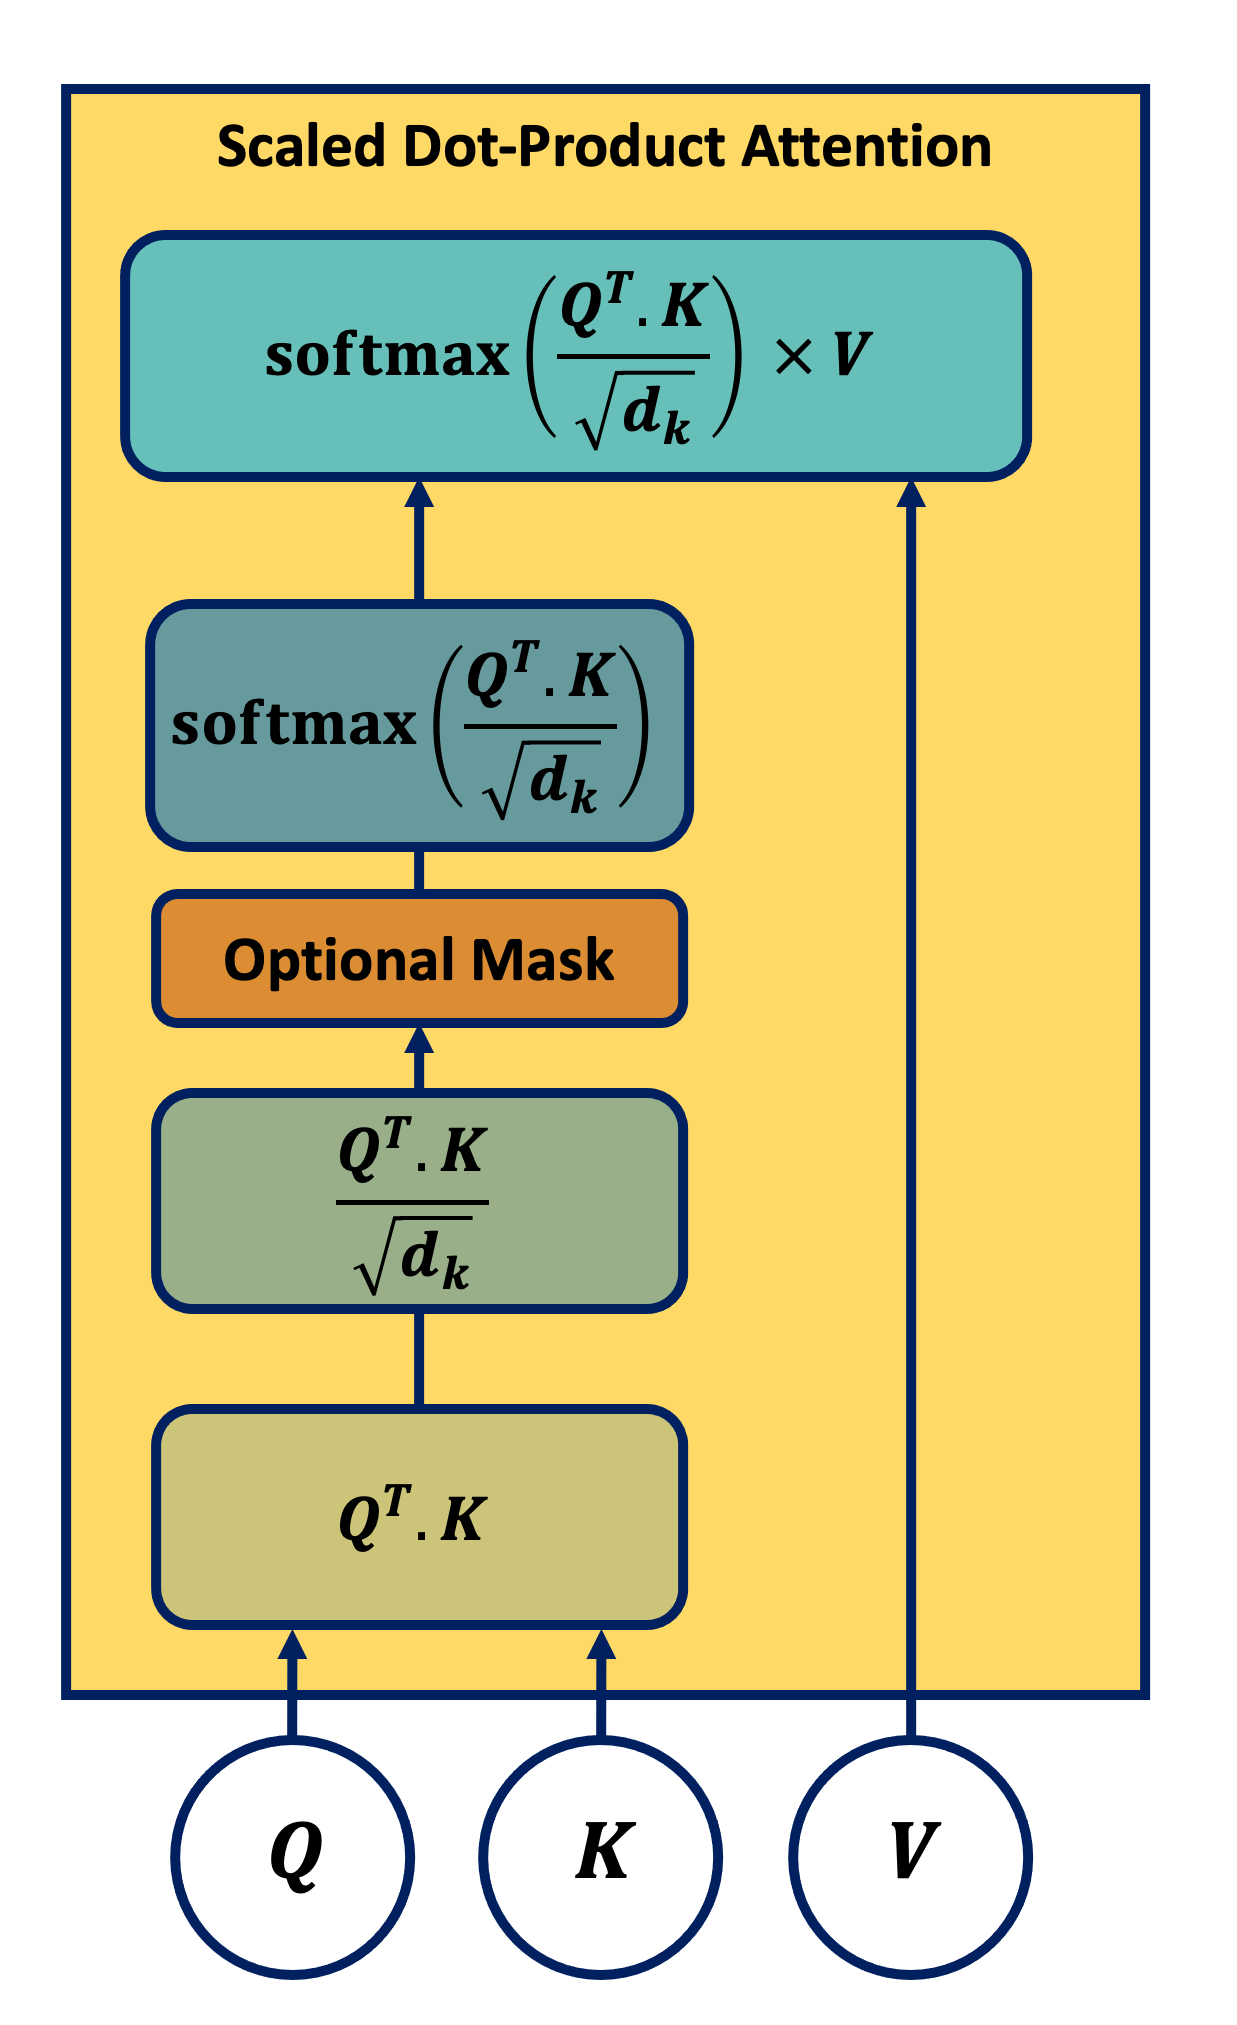
\includegraphics[scale=0.65]{Images/ML/scaledDotAtt.png}
        \caption{Scaled dot-product attention with optional masking.} 
        \label{fig:scaledDotAtt}
    \end{subfigure}
    \hfill
    \begin{subfigure}[b]{0.5\textwidth}
        \centering
        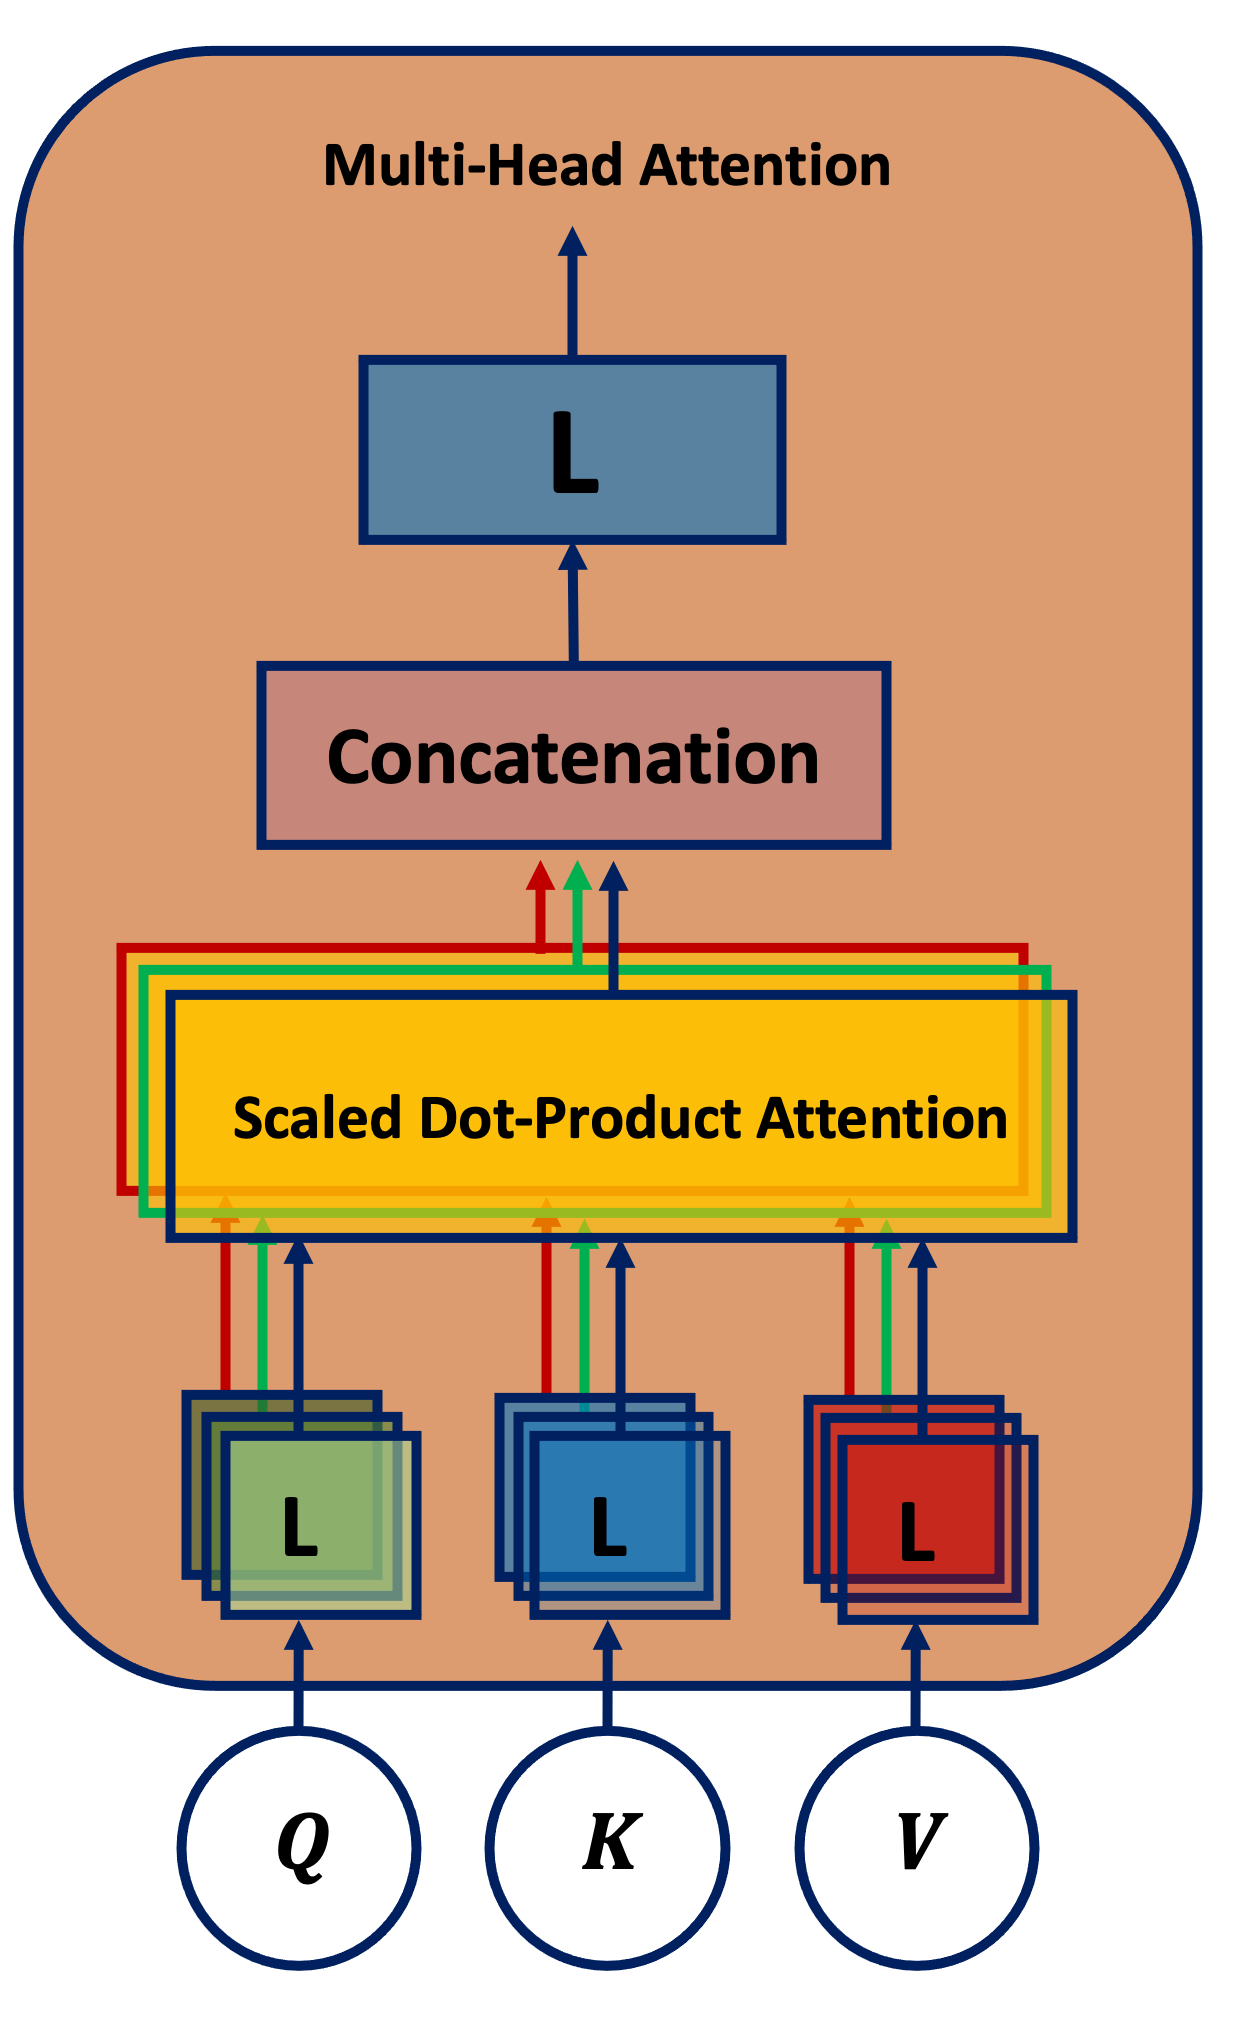
\includegraphics[scale=0.65]{Images/ML/multiHeadAtt.png}
        \caption{Multi-head attention module, where $L$ stands for a linear transformation of the input.} 
        \label{fig:mulitheadAtt}
    \end{subfigure}
    \caption{Multi-head attention mechanism in a transformer. The core operation is an optionally masked scalled dot-product of the queries $Q$, keys $K$, and values $V$. A head consists in three (optionally different) linear projection of the tuple $(Q, K, V)$, each leading to a separate scaled dot-product. The multi-head modules then concatenates all the different head results and finishes with another linear transformation.}
    \label{fig:transAtt}
\end{figure} 

\paragraph{Pros:}
\begin{itemize}
    \item \textit{Versatility:} The Transformer architecture has been successfully applied to various \gls{nlp} tasks - including machine translation, text summarization, and language modeling - and computer vision tasks.
    \item \textit{Parallelisation:} The architecture allows for efficient parallelisation of training, speeding up the learning process.
    \item \textit{Capturing Dependencies:} The self-attention mechanism enables the model to capture long-range dependencies in sequences.
    \item \textit{Stability:} per design Transformers benefit from regularisation effect due to residual connexions and normalisation layers. Models based on this structure can therefore scale to in complexity while resisting overtraining and with robust training conditions.
\end{itemize}

\paragraph{Cons:}
\begin{itemize}
    \item \textit{Computational Complexity:} Training large Transformer models can be computationally expensive, requiring powerful hardware.
    \item \textit{Interpretability:} The attention mechanism, while effective, can be challenging to interpret, making the model somewhat of a "black box."
    \item \textit{Data Dependency:} Transformer models may require large amounts of data for effective training, which may limit their application in domains with limited labelled data.
\end{itemize}

\section{Training and Optimising Deep Learning Models}
Training and optimising neural network models involve a combination of selecting appropriate architectures, fine-tuning hyperparameters - which cannot be learnt by backpropagation-, and employing acceleration techniques to improve efficiency and convergence. In this section, key aspects of the training process are explored, and acceleration techniques commonly used in practice are discussed.

\subsection{Training Algorithms}
When optimising the learnable parameters of a model, different training algorithms can be deployed to update the weights. All strategies are refinement on the base gradient descent rule of Equation \ref{eq:gradientdescent}, and each method has different advantages. The two main approaches are: 
\begin{itemize}
    \item \gls{sgd}: the update rule is the same as that of Equation \ref{eq:gradientdescent}, with the only difference being in how the gradient of the weights is computed. Instead of deriving it for the whole dataset (full-batch), the expectation over a random sub-batch is taken, hence the stochastic behaviour: \[ \nabla w = \frac{1}{b} \sum_{s=1}^b \nabla w_s,\] with $\nabla w_s$ being the gradients of the parameters computed for a single datapoint. A common observation is that for sub-batches - from now-on referred to as just \textit{batch} - of sufficient size, the stasticial estimator of the gradient based on the batch is unbiased. This greatly accelerates the time it takes to compute the gradient and naturally splits the loop over the dataset into different iterations called \textit{steps}, at which a batch is passed throught the network, a beneficial feature in the case of large datasets that would not fit in memory. This has also an effect on regularisation of the model, has each computed gradient on a batch has larger variance than a full-batch, making it harder for the model to overtrain. 
    \item Adam is an algorithm published in 2014 leveraging an adaptive moment estimation approach as well as batch processing \cite{adamPaper}. The moment in this sense is analoguous to the physical moment and encapsulates the dynamic of the optimisation as dervied by the gradient. The fundamental idea is that larger gradients indicate a steep slope that can be quickly traversed, so that any slowing down due to a changing curvature of the objective function landscape can be mitigated due to the inertia of the weights. This behaviour is implemented as an exponentially decaying moving average: the moment $m^t_w$ of weight $w$ at step $t$ is updated with a gradient forgetting factor $\beta_1 \in [0, 1[$ such that: \[ m_t \leftarrow \beta_1 m^{t-1}_w + (1 - \beta_1) \nabla_w \mathcal{L}^t,\] where the previous contribution are successively mutliplied by $\beta_1$ reducing the importance of earlier gradients progressively. Additionally, another element is taken into account in the gradient descent rule: the second moment $(\nabla_w \mathcal{L}^t)^2$. This tracks the magnitude of the gradient and, by multiplying the gradient update by a term inversely proportional to the second moment, accelerates the gradient updates in ``flatter'' regions of the objective landscape giving small gradient magnitudes with the term: \[ v_t \leftarrow \beta_2 v^{t-1}_w + (1 - \beta_2) (\nabla_w \mathcal{L}^t)^2,\] where a second moment forgetting factor $\beta_2 \in [0, 1[$ is introduced. To avoiding biasing the gradient update, both the momentum (first moment) and the second moment are corrected with \[\hat{m}^t_w \leftarrow \frac{m^t_w}{1 - \beta_1},\] and \[\hat{v}^t_w \leftarrow \frac{v^t_w}{1 - \beta_2}.\] The two contributions are then combined into a single gradient descent step following equation \ref{eq:adam}
    \begin{equation}\label{eq:adam}
        w^{t} \leftarrow w^{t-1} - lr \times \frac{\hat{m}^t_w}{\sqrt{\hat{v}^t_w} + \epsilon},
    \end{equation}
    where $\epsilon$ is added for numerical stability and is typically chosen to be a very small number to not bias the results.
\end{itemize}

A key hyperparameter in any gradient descent algorithm is the learning rate $lr$. There is no evident choice for this parameter and suitable values have to be derived on a case-by-case approach. A useful technique to let the training process converge to a good minimum of the loss function and avoid unsuitable local minima is to adapt a \textit{learning rate schedule}: the learning rate is modified throughout training to resolve different part of the loss function. Initially, having a relatively larger $lr$ allows the model to quickly update its weights in the direction of the minimum. If the rate is kept too high, the weights will not be able to approach the minimum and will overshoot or ``bounce' around the optimal set. In order to avoid this, the scheduler should reduce the learning rate so that smaller steps can be taken later in the training to approach the chosen optimum. At the beginning, the rate is typically not set to its maximum to start the gradient process in a valley of interest. An equivalent choice is to modify the batch size while keeping the $lr$ fixed \cite{smith2017decay}. This has also a regularising effect on the gradient: small batch sizes capture large variances and let the optimisation make drastic changes of orientation in the optimising function landscape, thereby avoid unsatisfactory local minima. Larger batch sizes stabilises the direction of descent, thereby offering a lower variance but potentially biased estimates towards a minimum. Combining these two characteristics at different epoch of the training is therefore an effective way to improve the training performance. Some methods, such as Adam, have other specific hyperparameters that should be optimised with the procedure described later in this chapter for hyperparameters.

\subsection{Regularisation}
Regularisation techniques are applied in the architecture and training procudure to prevent overfitting. Common methods include \textit{dropout}, which randomly drops connexions during training with Bernouilli probability distribution of parameter $p$, and L2 (L1) regularisations, which penalise large weights proportionaly to a penalisation parameter $\lambda$ times the sum of the squared (absolute value) of the weights. Both $p$ and $\lambda$ require careful optimisation as regularising the model can introduce bias and hit the overall performance. Additionally, batch normalisation is a technique that normalises the inputs of a layer over the batch, reducing internal covariate shifts. It helps stabilise and accelerate the training process. This is distinct from the layer normalisation used in the Transformer architecture of section \ref{sec:transformer} as the normalisation is carried over the batch samples rather than the activations. 

\subsection{Architecture \& Hyperparameters Optimisation}
There are several characteristics of the network that need to be optimised. Mainly: 
\begin{itemize}
    \item \textbf{Architecture Selection:} choosing the right architecture is crucial for the success of a \gls{nn}. Factors to consider include the complexity of the task, the nature of the data, and the desired trade-off between model complexity and interpretability. Limits in computing power should be factored in. Elements of the architecture include the type of \gls{ml} chosen (\gls{bdt}, \gls{dnn}, \gls{cnn}, \gls{rnn}, Transformer, ...), the choice of activation functions (\gls{relu}, tanh, ...), and the number of layers and nodes as well as connexions between the units.
    \item \textbf{Hyperparameter Tuning:} optimising hyperparameters - parameters that cannot be optimised with backpropagation of the gradients of the loss - is essential for achieving good model performance. Key hyperparameters include learning rate-related parameters, the batch size, and regularisation parameters.
\end{itemize}
The optimisation process for both hyperparameter tuning and architecture selection is expensive: it requires training and testing models with different combinations of hyperparameters or model architecture to evaluate their respective performance and uncover the best peforming options. Techniques such as grid search, random search, and Bayesian optimisation can be employed to efficiently explore the hyperparameter space. Architecture search is usually performed by trials and attempts, and the literature offers insights and guidance into what models might best perform in specific situations. 

\subsection{Acceleration Techniques}
Training an \gls{ml} model is often a computationally demanding tasks that can be carried out more effectively on specifically designed hardware and with some tricks in the process. 
\begin{itemize}
    \item \textbf{Parallel Dataloading:} loading data in parallel can significantly speed up the training process. Libraries like TensorFlow and PyTorch provide functionalities for efficient parallel dataloading. Instead of preparing a single batch, multiple batches can be loaded by different processing units in parallel to avoid this step becoming a bottleneck in performance. 
    \item \textbf{Early Stopping:} to prevent overfitting and save computation time, early stopping involves monitoring the model's performance on a validation set and halting training when performance ceases to improve.
    \item  \textbf{Hardware Accelerators:} specialised hardware accelerators can further accelerate training. The \gls{gpu} architecture is design to perform simple mathematical operation in parallel. This is precisely the needs of \gls{nn} optimisation, as each computational step consists in a matrix multiplication. Utilising \gls{gpu} for training and inference can give substantial speedups compared to \gls{cpu}-based computing. Other types of hardware optimised for \gls{dl} include the Tensor Processing Units (TPU) and the Neural Processing Units (NPU). 
    \item \textbf{Transfer Learning:} transfer learning leverages pre-trained models on large datasets and applies them to a new task. The idea is that there are some fundamental simularities between the new task and the task used to train the fondational model that will let this latter one start with useful information. Fine-tuning these models on specific tasks can significantly reduce the required training time and data compared to training a model from scratch. This approach is becoming increasingly fashionable, as larger \textit{foundational} models trained on multiple tasks with huge datasets can then be applied to a specific task, with the pre-trained weights either kept fixed or free to be modified to optimise the new task. New modules can also be added on top the foundational model to specialise it to a specific use-case. Such large foundational models are already available in \gls{nlp} (e.g., the Mistral 7B \cite{jiang2023mistral} - a 7 billion parameters Transformer capable of analysing English sentences and code) and computer vision (e.g., the Florence-2 model by Microsoft \cite{xiao2023florence2} - built on a Transformer with 0.5 billion parameters).
\end{itemize}
Training and optimizing deep learning models involve a combination of careful architectural choices, hyperparameter tuning, and the use of acceleration techniques. Selecting the most appropriate techniques is a task-specific challenge that will further depend on available resources and the desired trade-offs between training time and model performance as well as interpretability.


\newpage
\chapter{\color{oxfordblue} Flavour Tagging}\label{chap-ftag}
\ChapFrame

\textit{
The focus of this chapter is on an essential task in the ATLAS experiment: identifying particles flying through the detector. This objective of assigning labels to reconstructed particles from measurements is referred to as tagging. An important family of particules to be tagged are quarks, and disentangling which specific flavour of the quarks should be assigned to an observed signal is called flavour tagging. Free quarks and gluons hadronise as per the rules of \gls{qcd}, forming large number of particles that can themselves further decay. Such a dynamic results in a many particles radiating within a clone centred around the inital flavoured particle, a structure referred to as a jet. Consequently, this chapter introduces method to tag jets, as labelled by the flavour of the initial parton. In particular, the different algortihms and methods relevant for this task developped during the during of the author's contribution to ATLAS are reviewed, with the first trainings of DIPS, DL1d, GN1, and GN2 described in details as well as early studies of the hyperparameter optimisation of GN2.
}

\section{Heavy-Flavour Jet Tagging}
A fundamental ingredient in any ATLAS analysis is the ability to correctly identify particles in the aftermath of a collision, from $\tau$-leptons, to $b$- and $c$-quarks, and gluons $g$. Having well-calibrated and optimally performing b- and c-tagging tools is of primary importance in studies of the Higgs boson couplings to $b$- and $c$-quarks. It is also critical for top $t$-quark measurements and searches for extensions of the \gls{sm}. As described by the theory of \glsfirst{qcd}, colour-charged objects, such as a $b$- or a $c$-quark, undergo hadronisation to form collections of colourless hadrons. These hadrons, mostly $B$ for $b$-quark and $D$ for $c$-quark, are quasi-stable and further decay in the volume of the detector. Such a succession of decays leaves a collection of particles within a cone oriented in the direction of the original parton, an easily recognisable pattern referred to as a \textit{jet}. From an analysis of the complicated structure of the jet, the flavour of the initially decaying particle can be reconstructed. The labelling scheme applied to jet consist in identifying the hadron associated to the jet: a $b$-jet must contain at least one $b$-hadron, a $c$-jet at least one $D$-hadron and no $b$-hadron, and if none of these hadrons are found the jet is said to be a light-jet, thereby grouping $u$-, $d$-, and $s$-quarks with gluons $g$. This is the task of \textit{flavour tagging}, and the tool to achieve this identification is called a \textit{tagger}. \\

\subsection{Decay Topology}
When a $b$-quark is produced, such as in the aftermath of a hard scatter due to a proton-proton collision, it quickly undergoes the process of hadronisation to neutralise its free colour-charge. This process leading free quarks and gluons to a final state of hadrons and leptons is intrinsically non-perturbative and can only be described with phenomenological models of framgentation \cite{Webber:419784}. The family of $b$-hadrons is composed of different ensemble of a bottom quark $b$ with one or more light quarks. These include the $B$-mesons, mainly $B^0=d\bar{b}$, $B^-=\bar{u}b$, $B^+=u\bar{b}$, and the strange and charmed $B$-mesons, and baryons, such as the $\Lambda_b^0=udb$ \cite{ATL-PHYS-PUB-2014-008}. For $b$-quarks, the hadronisation process is hard and most ($\sim$ 70-80\%) of the quark momentum is passed to the $b$-hadron \cite{Webber:419784}. Tagging $b$-jets benefits from a particularly advantageous configuration: the $b$ is the lightest element of the third generation of quarks and must decay through a flavour-changing process through the weak interaction. Because of the relatively small \gls{sm} value of the $V_{bc}$ \gls{ckm} matrix element, decay processes involving a transition $b \rightarrow c$ are suppressed, giving $b$-hadrons a characteristically long proper lifetime $\tau_B \approx 1.5$ ps corresponding to a proper decay length $c\tau_{B} \sim 450$ $\mu$m \cite{Tanabashi:2018oca}. In the laboratory frame and considering the boost of the $b$-hadron given by a Lorentz $\gamma$ factor ($\gamma > 1$) and $\beta = v/c \approx 1$ in the high energy limit, the distance travelled is given by \[d = \gamma \beta c \tau_B \approx \gamma c \tau_B.\] In the high-energy limit, $\gamma \approx E_B / m_B$, where the mass of $B$-hadrons is in the range 5-6 GeV. Consequently, a 50 GeV $b$-hadron decays at a distance of $d \approx 4.5$ mm from the primary vertex which can be resolved. This distance travelled, also called the $b$-hadron radius $L_{xy}$, further increases with jet $p_T$ and at transverse momentum above $\sim$500 GeV even overpasses the first detector layer of the \gls{ibl}, located at a distance of roughly 33 mm from the centre of ATLAS as shown in Figure \ref{fig:bhaddecay}. The location of the $b$-hadron decay can often be reconstructed by the ATLAS detector, and the reconstructed point of decay is called \gls{sv} \cite{Aad:2019aic}. Some important variables describing the decay of $b$-hadrons are the \glspl{ip} $d_0$ and $z_0$ of the charged particles emanating from the \gls{sv}. As shown in Figure \ref{fig:bjet}, $d_0$ and $z_0$ are the transversal and longitudinal distances from the primary vertex to the perigee\footnote{The point of closest approach.} of the track associated with the charged particle. For a $b$-jet, the \glspl{ip} can be large thanks to the long lifetime of the associated hadron. On average, a $b$-hadron decays weakly to four or five charged stable particles \cite{ATL-PHYS-PUB-2014-008}. Another characteristic of $b$-jets is the likely presence of leptons in the jet cone, as 40\% of the decays of $b$ and $c$-hadrons are semi-leptonic and include either an $e$ or a $\mu$ \cite{Tanabashi:2018oca}. \\

\begin{figure}[h!]
\center
\begin{subfigure}[b]{0.48\textwidth}
  \centering
  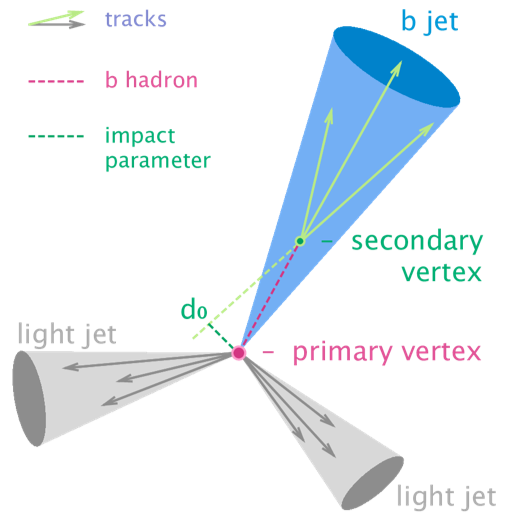
\includegraphics[width=0.9\textwidth]{Images/bjet}
  \caption{Representation of a $b$-jet \cite{bjetimage}.}
  \label{fig:bjet}
\end{subfigure}
\begin{subfigure}[b]{0.49\textwidth}
  \centering
  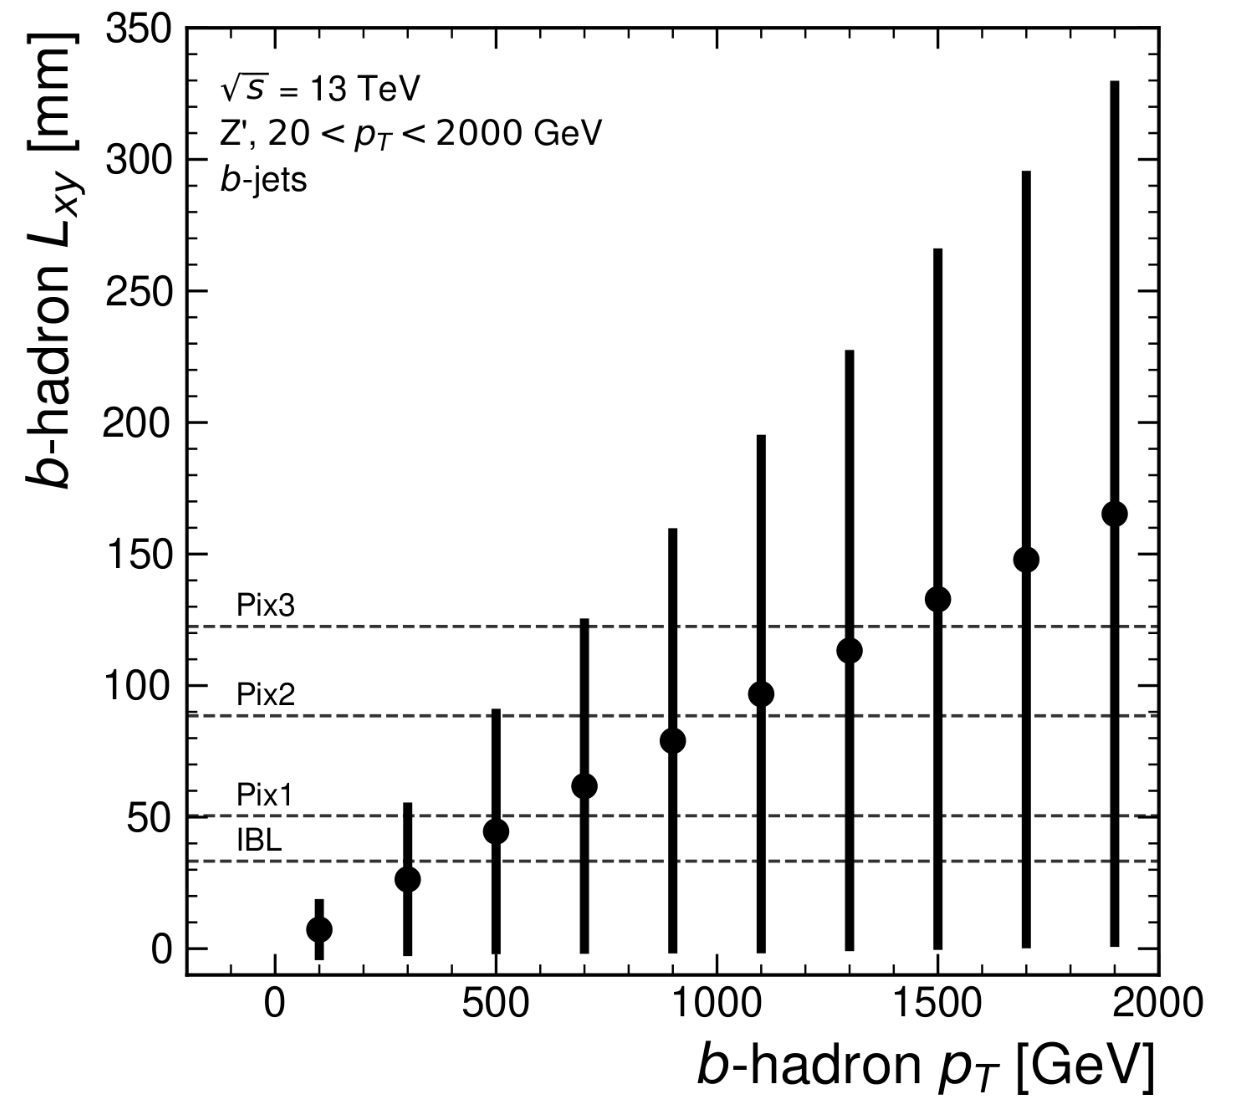
\includegraphics[width=0.98\textwidth]{Images/FTAG/intro/bhaddecay.png}
  \caption{$b$-hadron decay radius as a function of jet $p_T$ reconstructed for $b$-jets in a $Z'$ events with the IBL and pixel layers indicated, from \cite{VanStroud:2869719}. Error bars show the standard deviation of $L_{xy}$ in each $p_T$ bin.} 
  \label{fig:bhaddecay}
\end{subfigure}
\end{figure}

While $b$-jets benefit from an advantageous topology, tagging $c$-jets proves much more challenging as they are at an intermediate scale between light- ($u$, $d$, $s$, and gluons) and heavy flavour jets. A $c$-jet must contain at least one $c$-hadron, from either a $D$-meson (e.g., $D^+=c\bar{d}$, $D^-=d\bar{c}$, $D^0=c\bar{u}$) or a $c$-baryon (e.g., $\Lambda_c^+:udc$). The average decay length for charged (neutral) $D$-mesons, $c\tau_D \sim 300$ $(100)$ $\mu$m \cite{Tanabashi:2018oca}, is smaller than for $b$-hadrons and is harder to resolve with the currently deployed tracker. The decay chain of $b$-hadrons often includes a $c$-hadron, making a clean separation of $c$-jets from $b$-jets harder. Compared to $b$-jets, $c$-jets have a lower final state charged particle multiplicity, on average 4. This lets $\tau$-jets easily being mistaken for $c$-jets, as these leptons can hadronically decay into a similar number of particles to mimic a jet in the detector. For all these reasons, less effort has been historically dedicated to constructing $c$-taggers in ATLAS. The task is however gaining particular attention due to the focus on the challenging $H \rightarrow c\bar{c}$ search \cite{Aaboud:2018fhh, Collaboration:2721696, arXiv:2205.05550}. The focus of this chapter is on the development of novel taggers to identify $b$- and $c$-jet for the ATLAS experiment during the 2020-2024 period, overlaping with the end of Run 2 (2015-2018) analyses and the begining of Run 3 (2022-2026).

\subsection{Flavour Tagging at ATLAS}
In the ATLAS experiment, a choice was made to develop centrally a tagger to be used by the whole collaboration. It relies on a dedicated set of algorithms to perform simultaneously $b$- and $c$-tagging and is continuously improved to meet the requirements of the physics program. Currently, all adopted approaches rely on \gls{dl} methods, given their vastly superior effectiveness. This area of research has been evolving rapidly in recent times due to the community adopting advanced methods from the field of \gls{ai}. As such, various models have been introduced and the last two generations can be split into two categories: 
\begin{enumerate}
  \item The DL1 family are \gls{dl} models built in a hierarchical way. These \gls{dl} methods rely on high-level features reconstructed by sub-algorithms based on physics variables, such as the tracks \glspl{ip}, and the reconstruction of secondary vertices \cite{ATL-PHYS-PUB-2015-022}. The most important models in this family are those including a \gls{dl} sub-model to analyse tracks with either a \gls{rnn} approach for \gls{dl1r} \cite{ATLAS:2017bcq}, leveraging the \gls{rnnip} sub-tagger \cite{ATL-PHYS-PUB-2017-003}, and a Deep Set approaches for \gls{dl1d}, leveraging the \gls{dips} sub-tagger \cite{ATL-PHYS-PUB-2020-014}. This last tagger is, at the moment of writing this thesis, the state-of-the-art deployable tagger for ATLAS in the ATLAS software \cite{ATL-SOFT-PUB-2021-001}. Algorithms from this family were developped for Run 2 of the ATLAS experiment \cite{atlas:FTAGRUN2}, with \gls{dl1d} behind developped towards the end of this data campaign.
  \item The GN family of taggers are built on more advanced \gls{dl} method, as they move away from the hierarchical approach of the DL1 family and directly analyse track and jet information in a unique complex architecture. The GN family is based either on a full Graph Attention Network (\gls{gat}) for \gls{gn1}, and a Transformer encoder for \gls{gn2} \cite{ATL-PHYS-PUB-2022-027, ATL-PLOT-FTAG-2023-01, duperrin2023flavour}. This lighter algorithm pipeline greatly simplifies the maintenance and turnaround time for modification, making the process of updating the taggers nimbler and easier to tailor to specific applications. The GN taggers greatly outperform the DL1 family and represent an exciting area of progress for future analysis requiring precise flavour jets tagging. These methods are being integrated in the ATLAS software stack with objective to be integrated in analyses of the ongoing Run 3 \cite{ATL-SOFT-PUB-2021-001}.  
\end{enumerate}

\begin{figure}[h!]
  \center
  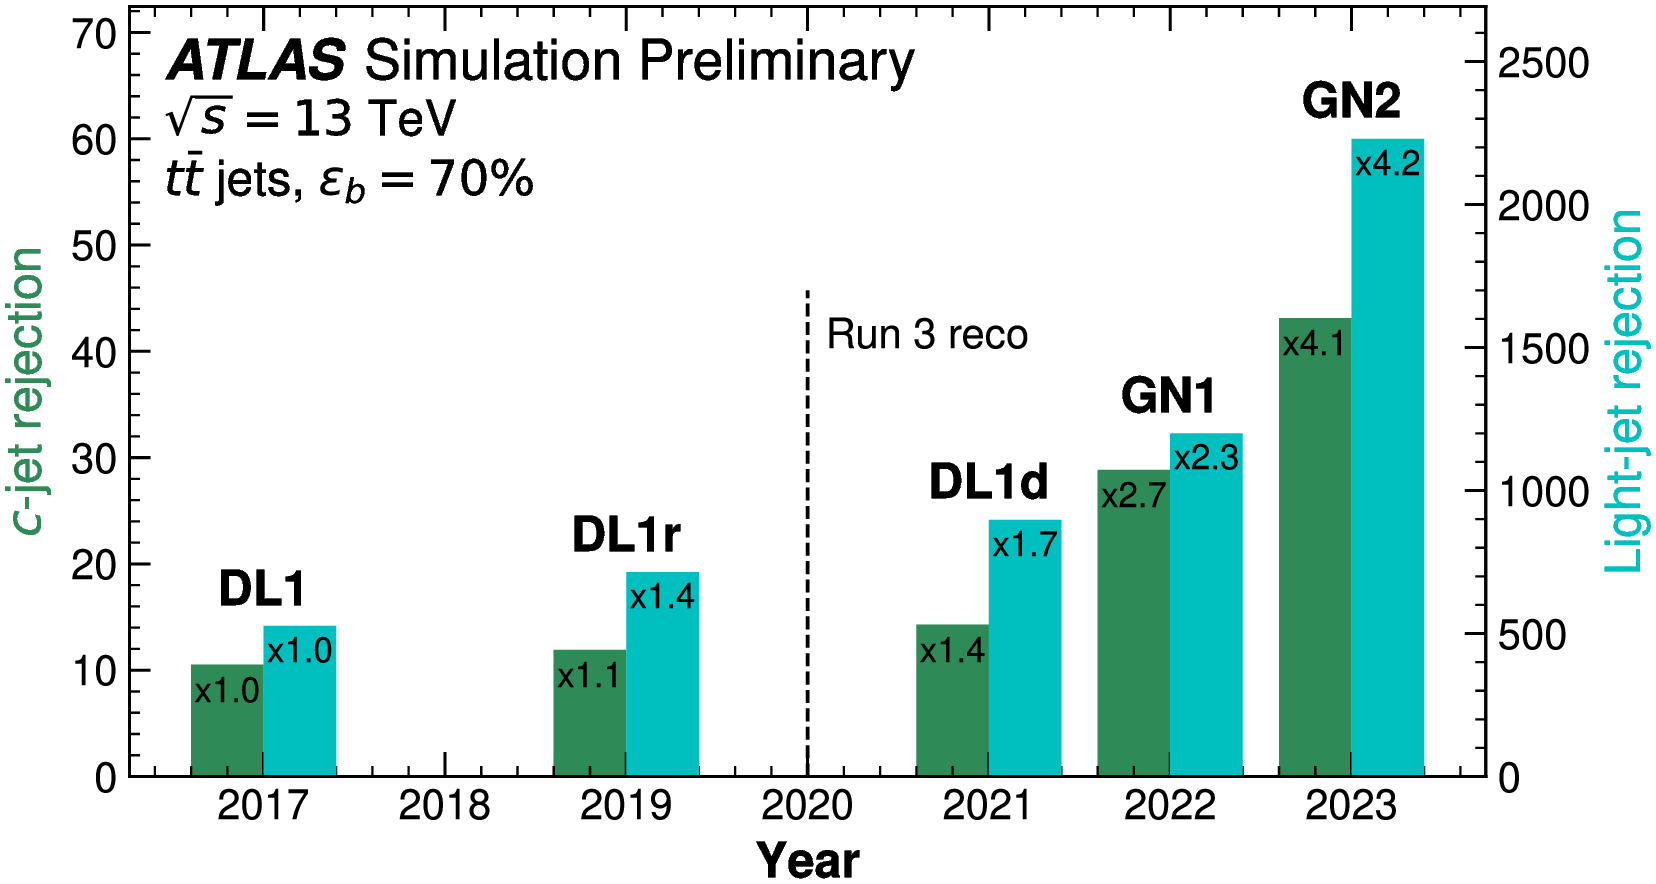
\includegraphics[width=0.8\textwidth]{Images/FTAG/storyFtag.png}
  \caption{Comparison of the performance of flavour tagging models introduced through the years, from \cite{ATL-PLOT-FTAG-2023-01}. Light and $c$-jet rejections are plotted for different taggers at a fixed $b$-jet tagging efficiency of 70\% on a common $t\bar{t}$ evaluation sets. The multiplicative factors in the bars are with respect to the bare DL1 model performance.} 
  \label{fig:storyFtag}
\end{figure}

A historical perspective on the evolution of performance for the different taggers mentioned is presented in Figure \ref{fig:storyFtag}, showing a remarkable continuous increase in light- and $c$-jet rejections at a fixed $b$-tagging efficiency of 70\% on a $t\bar{t}$ dataset. The analysis presented in the latter part of this thesis was carried out in the span of 2021-2024, and was therefore restricted to tools and methods available to the experimental team during this period. As such, due to the need to calibrate the GN taggers as explained latter in Section \ref{chap-calibration} of this chapter, the second family of taggers based on graphs was not yet ready for deployement, making the first family still relevant to explore. Furthemore, some specialised use of flavour taggers and early Run 3 analyses still required the DL1 family, such as the $X_{bb}$ tagger identifying pairs of $b\bar{b}$ and $c\bar{c}$ produced by heavy resonance decays such as a Higgs or a $W$, as described in Section \ref{chap-GN2X}. All the taggers described in this chapter have been integrated in the ATLAS software \cite{ATL-SOFT-PUB-2021-001}. Some early studies of the future performance of the \gls{dl1d} and \gls{gn1} taggers with the updated \gls{itk} detector at the high-luminosity \gls{lhc} as been performed in Ref \cite{ATL-PHYS-PUB-2022-047}.

\subsection{Datasets}\label{ftagdatasets}
The $p_T$ spectrum studied by ATLAS covers a wide range of energies, extending up to 7 TeV. In order to train models able to perform on this large phase space, two datasets are typically combined and described in this section. Each dataset is based from simulated proton-proton collisions at a centre of mass energy $\sqrt{s}$ = 13 TeV. The lower $p_T$ phase space is simulated with the \gls{sm} top-antitop quark pair production $t\bar{t}$ process with at least one $W$ boson produced decaying leptonically, while a \gls{bsm} $Z'$ process is used for the higher momentum region. The latter simulates a modified $Z$ boson from the \gls{sm} with an increased mass to generate a relatively flat jet $p_T$ spectrum of up to 6 TeV. This $Z'$ boson decays in similar proportions to a pair of $b$, $c$, and light-jets. All simulations include realistic effects present in the real data, such as multiple proton-proton interactions per bunch crossing, so-called \glsfirst{pu}, with an average value of $\mu = 40$. Other effects including in the simulations are the detector response from prior and posterior bunch crossing (in-time pile-up) as well the activity from the rest of the event (underlying event). \\

Events in the $t\bar{t}$ samples are simulated using \uppercase{POWHEGBOX V2} generators to next-to-leading (NLO) order in the strong coupling constant $\alpha_s$ \cite{PaoloNason_2004, StefanoFrixione_2007, StefanoFrixione_20072, POWHEGBOX}. The hard scatter matrix element is computed for proton-proton collision with the \uppercase{NNPDF3.0NNLO} set of parton distribution functions (PDF) \cite{PDFLHCrun2}, and the simulated hard scatter events are interfaced with \uppercase{PYTHIA 8.230} \cite{SJOSTRAND2015159} using the A14 parameter tune \cite{ATL-PHYS-PUB-2014-021} and the \uppercase{NNPDF2.3LO} PDFs for the parton shower, hadronisation, and underlying event simulations \cite{BALL2013244}. Studies in Refs \cite{ATL-PHYS-PUB-2016-020, ATL-PHYS-PUB-2020-023} showed these to be the optimal choice to correctly model the top quark $p_T$ and the number of additional jets in the event, with the $h_{\textrm{damp}}$ parameter set at 1.5 the mass of the top-quark $m_{\textrm{top}} = 172.5$ GeV. The $Z'$ events are fully simualted with \uppercase{PYTHIA 8.212}, A14 tune and the \uppercase{NNPDF2.3LO} PDFs. The decays of $b$- and $c$-hadrons are performed by \uppercase{EvtGEN} v1.6.0 \cite{LANGE2001152}. \\

The detector reconstruction effect of ATLAS and the modelling of the interaction between long-lived hadrons and the detector material are simulated with a dedicated software \cite{ATLASSimulationInfra} built on GEANT4 \cite{Agostinelli:602040}. Jets are selected in the phase space region defined by $|\eta| < 2.5$ and $p_T > 20$ GeV, with no overlapping with prompt generator-level $e$ or $\mu$ from the $W$ decay allowed. Pile-up contamination is further reduced by an additional standard selection using the \glsfirst{jvt} algorithm at a tight working point for jets with $p_T < 60$ GeV and $|\eta| < 2.4$ \cite{ATLAS-CONF-2014-018}. Tracks are associated to jets using a $\Delta R$ association cone of width decreasing with $p_T$ ($\Delta R \approx 0.45$ at $p_T =$ 20 GeV and $\Delta R \approx 0.25$ at $p_T > 200$ GeV). Tracks within the cones of several jets are associated to jet with minimal $\Delta R(\textrm{track, jet})$. The label of the jet is inferred from the presence of a truth-level hadron within the cone $\Delta R(\textrm{hadron, jet}) < 0.3$ centred around the jet axis.

\section{DL1 Family of Models: DL1r \& DL1d}
This family of tagger is built with a hierarchical approach, combining low-level algorithms that are independentely optimised into a final \gls{dnn} network of a few layers to output a final prediction. Not all low-level modules are based on \gls{dl}, with some instead directly implementing physics-motivated algorithms. They consist of \cite{Paganini:2289214, atlas:FTAGRUN2}:
\begin{itemize}
  \item \gls{ip} likelihood: IP2D and IP3D are likelihood-ratio templates in 2D and 3D to assign flavour-discriminating weights based, respectively, on the transversal and global impact parameters significance (corresponding to the reweighted \gls{ip} variables by their respective uncertainties) $S_{d_0}$ (35 bins) and $S_{z_0}$ (20 bins) of the tracks, and 14 bins of track catogarisation for IP3D \cite{ATLAS:2017bcq}. For the three flavours, this results in $35 \times 20 \times 14 \times 3 = 29,400$ final bins, which each probability being computed per track. The likelihood assigned to the jet assumes the tracks are independent and is therefore calculated as the product of the per-track likelihoods. A discriminant is derived from the conditional log-likelihood, e.g., $D^b_{IP3D,f} = \sum_{i \in \textrm{tracks}} \log\frac{p_b^i}{p_f^i}$, with $f= c$ or light \cite{ATL-PHYS-PUB-2015-022}.
  \item Track collection analyser: either with \gls{rnnip} \cite{ATL-PHYS-PUB-2017-003} or \gls{dips} \cite{ATL-PHYS-PUB-2020-014}. These are \gls{dl} approaches to extract discrimination information on the set of tracks associated with a jet. These taggers are further described later in this chapter.  
  \item \gls{sv1}: combining a secondary vertex finder and a tagger to offer flavour discrimination information \cite{atlas:FTAGRUN2}. The former, based on the VKalVrt vertex reconstruction package \cite{Kostyukhin:685551}, returns a list of candidate secondary vertices with measured quantities assigned to each vertex. The latter derives jet weights based on discriminative variables and computes properties of the \gls{sv}, such as the mass. 
  \item Jet Fitter: a vertexing algorithm based on a Kalman filter to reconstruct the topology and fit the decay chain \gls{pv} $\rightarrow$ $B$ $\rightarrow$ $D$ with the assumption that the vertices of the weakly decaying B/D-hadrons tend to align with the \gls{pv} \cite{atlas:FTAGRUN2, ATL-PHYS-PUB-2018-025}. 
\end{itemize}

\begin{figure}[h!]
  \centerline{
  \begin{minipage}[c]{0.4\textwidth}
      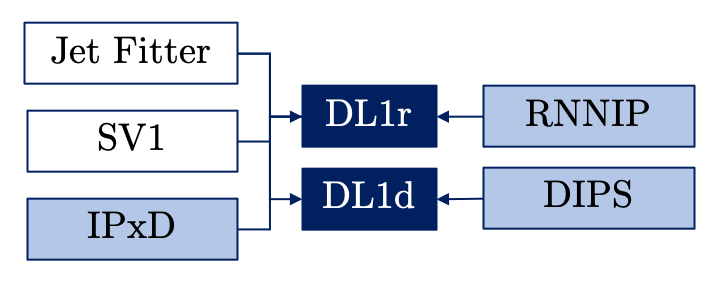
\includegraphics[scale=0.5]{Images/Algorithms}
    \end{minipage}
  \begin{minipage}[c]{0.6\textwidth}
      \caption{The algorithms for flavour tagging at ATLAS. High-level taggers are in dark blue, track-based taggers in light blue and vertex-related taggers in white.}
      \label{fig:algo}
    \end{minipage}
  }
\end{figure}

The outputs of these low-level algorithms, as well as certain jet-related variables, such as $p_T$, are then combined as input to a high-level tagger consisting of a fully-connected \gls{nn} called \gls{dl1r} or \gls{dl1d}, respectively if \gls{rnnip} or \gls{dips} is used. The input vector is typically made of 44-45 features. This high-level tagger outputs three probabilities $p_X$ for the analysed jet to correspond to a $b$-, $c$-, or light--flavour (indicated with the letter $u$) such that $p_b + p_c + p_u = 1$. A $b$-tagging score $D_b$ is then derived by computing a scaled log-likelihood ratio: 
\begin{equation}\label{bdisc}
D_b = \log \frac{p_b}{f^b_c \times p_c + (1 - f^b_c) \times p_u},
\end{equation}
where $f^b_c$ is the charm fraction, a parameter that can be modified to tweak the importance of each flavour. The analogous $c$-tagging score $D_c$ is: 
\begin{equation}\label{cdisc}
D_c = \log \frac{p_c}{f^c_b \times p_b + (1 - f^c_b) \times p_u}.
\end{equation}

A jet is $X$-tagged if the $D_X$ discriminant score is above a set threshold constant $c_{wp}$, defining a \gls{wp} with a unique configuration of signal and background (mis-tag) efficiencies. In this context, the efficiency $\epsilon^X_Y$ for $Y$-flavour jets to be $X$-tagged and the corresponding rejection $\mathcal{R}^X_Y$ are respectively defined as:
\begin{equation}
\epsilon^X_Y = \frac{N^{X-tagged}_{Y-jets}}{N_{Y-jets}} \quad \textrm{and} \quad \mathcal{R}^X_Y = \frac{1}{\epsilon^X_Y},
\end{equation}
where $N^{X-tagged}_{Y-jets}$ and $N_{Y-jets}$ are respectively the number of $X$-tagged $Y$-flavoured jets and the total number of $Y$-flavoured jets. The $f$-rejection is the inverse miss-tagged efficiency of flavour $f$.  \\

These high-level models are trained on \gls{mc} simulated data samples, as mentioned in Section \ref{ftagdatasets}, and need to be calibrated on real data to deliver an unbiased estimate, by deriving \glspl{sf} weights correcting the predictions for each jet as described in Section \ref{chap-calibration}. Uncertainties are derived on the predicted score and passed along to analyses using the tool. The novel algorithm of this family introduced in this work is the \gls{dl1d} tagger, which relies on the \gls{dips} sub-tagger to extract correlations between the tracks.  

\subsection{RNNIP}
The \gls{rnnip} tagger runs on arbitrary-length input sequences made of track features, as ordered by the absolute transverse \gls{ip} significance $|S_{d_0}|$, to extract tagging information from correlations between tracks \cite{ATL-PHYS-PUB-2017-003}. The vector of track features, described in greater details in Table \ref{tab:rnnipVar}, includes the transverse and longitudinal impact parameter significances, the jet $p_T$ fraction carried by the track, the distance between the track and the jet axis, and a learned 2D embedding of the track quality \cite{Paganini:2289214}. It outputs a probability $p_X$ for the jet to belong to flavour $X$ $\in$ [$b$, $c$, light, $\tau$].

\begin{figure}[h!]
  \center
  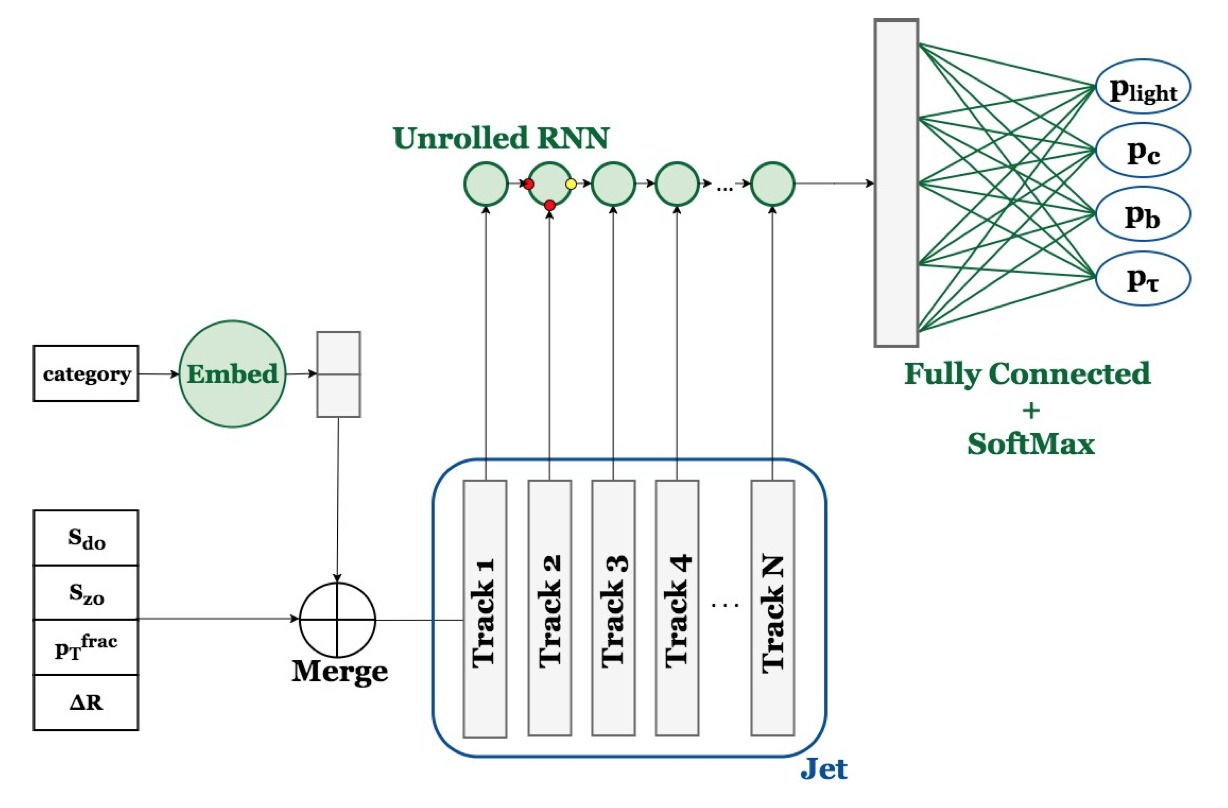
\includegraphics[scale=0.6]{Images/FTAG/rnnip_structure.png}
  \caption{Diagram of the \gls{rnnip} tagger for flavour tagging, from \cite{Paganini:2289214}. The input consists in track features augmented with an embedding of track categories. Tracks are then ordered by absolute transverse \gls{ip} significance and fed through an \gls{lstm} core. The unrolled sequence outputed from this \gls{lstm} is padded to a fixed size and processed by a \gls{dnn} to output the per-flavour probabilities.} 
  \label{fig:rnnipModel}
\end{figure}

The architecture of \gls{rnnip} is a \gls{rnn}-based model leveraging an \gls{lstm} core, as depicted in Figure \ref{fig:rnnipModel}. The arbitrary-length sequence fed as input is mapped by the \gls{lstm} cell with a 100-unit hidden layer into a 50-dimensional vector. This vector is then processed by a 20-unit fully-connected feed-forward neural network outputing the per-flavour probabilities by computing the softmax of the last layer's output. To avoid overfitting, a dropout value of 0.2 is applied to the \gls{lstm} cell. 

\begin{table}[h]
  \begin{center}
      \begin{tabular}{C{3cm}|C{13cm}} 
      	 \hline \hline
          Track Variables & Description  \\ \hline \hline
          $S_{d_0}$      & Lifetime signed transverse \gls{ip} significance $d_0 / \sigma_{d_0}$, with $d_0$ the transverse \gls{ip} - the transverse distance from the \gls{pv} to the point of closest approach (perigee) of the track - and $\sigma_{d_0}$ the error on $d_0$. If the perigee is in front (behind) the \gls{pv} with respect to the jet direction, the sign is positive (negative). \\ \hline
          $S_{z_0}$      & Lifetime signed longitudinal \gls{ip} significance $z_0 / \sigma_{z_0}$, with $z_0$ the longitudinal \gls{ip} - the longitudinal distance from the \gls{pv} to the perigee of the track - and $\sigma_{z_0}$ the error on $z_0$. A sign is assigned as per the prescription of $S_{d_0}$. \\ \hline
          $p_T^{\textrm{frac}}$   & Fraction of the reconstructed jet $p_T^{\textrm{jet}}$ carried by the track $p_T^{\textrm{frac}} = p_T^{\textrm{track}} / p_T^{\textrm{jet}}$. \\ \hline
          $\Delta R$(track, jet) & Geometrical distance in 2D angle between the track direction and jet axis $\Delta R = \sqrt{(\phi_{\textrm{track}} - \phi_{\textrm{jet}})^2 + (\eta_{\textrm{track} - \eta_{\textrm{jet}}})^2}$. \\ \hline
          Category       & 2D representation of the track quality learnt by an embedding layer. The categorisation is based on the number of observed, expected and missing hits in the different layers of the tracker (silicon pixel and strip detectors) \cite{ATL-PHYS-PUB-2015-022}.  \\ \hline
      \end{tabular}
    \caption{Track variables passed to the initial version of the \gls{rnnip} model \cite{ATL-PHYS-PUB-2017-003}. Later versions removed the category embedding and added the per-track hit information shown for \gls{dips} in Table \ref{tab:dipsVar}.}
    \label{tab:rnnipVar}
  \end{center}
\end{table}

\gls{rnnip} is designed to capture correlations between the tracks of a jet, a rich information explicitely missing from the \gls{ip}-based discriminant of IP2D and IP3D due to the factorisation of the likelihood. Some degree of correlation is expected between tracks, as these can emerge from the same secondary or tertiary vertex of the displaced decay in $b$- and $c$-jets. It removes the cumbersome procedure to built likelihood templates, which demands large amount of data to scale to finer bin resolution and is computationally expensive due to the number of bins scaling exponentially with the number of variables. Early tests showed that \gls{rnnip} is effective at building a discriminant, delivering superior performances to the \gls{ip}-based approaches with only $\sim$40 \% of the parameters - 11,636 trainable parameters for \gls{rnnip} \cite{Paganini:2289214}.

\subsection{DIPS}
The \gls{dips} tagger, based on the Deep Set architecture \cite{NIPS2017f22e4747} and depicted in Figure \ref{fig:dipsModel}, is a \gls{gnn}-based alternative approach to \gls{rnnip} to model the correlations between an arbitrary number of tracks \cite{ATL-PHYS-PUB-2020-014}. As introduced in Chapter \ref{chapter-GNN}, such a model is composed of two fully-connected feed-forward neural network. A first \gls{dnn} called the \textit{track network} $\Phi$ maps each individual track feature vector - similar to the input of \gls{rnnip} - to a latent space representing the nodes of a graph. The representations of each track in this latent space are then pooled by a simple summation operation - representing the unweighted edges of a fully connected graph - and given as input to a secondary \gls{dnn}, called the \textit{jet network} $F$, outputting the predicted probability $p_X$ for the jet to belong to flavour $X$ $\in$ [$b$, $c$, light, $\tau$]. This last network represents the global attribute of the graph $u$, in the notation of Chapter \ref{chapter-GNN}. 
In summary, \gls{dips} computes the following equation on the set of track features $\{ p_i \}$, with $i = 1, ..., N$ for arbitrarily-sized jets of $N$ tracks:
\begin{equation}
  DIPS( \{p_1, ..., p_N \} ) = F\left( \sum_{i=1}^N \Phi(p_i) \right),
\end{equation}
to output the per-flavour probabilities. The separation of computation into a per-track embedding and a per-jet processing after a size-indepent pooling performed by the sumation operator allows the model to process unordered sets of variable size. The track features used as inputs are described in Table \ref{tab:dipsVar}, with only the top 15 tracks as ranked by decreasing $S_{d_0}$ being kept.

\begin{figure}[h!]
  \center
  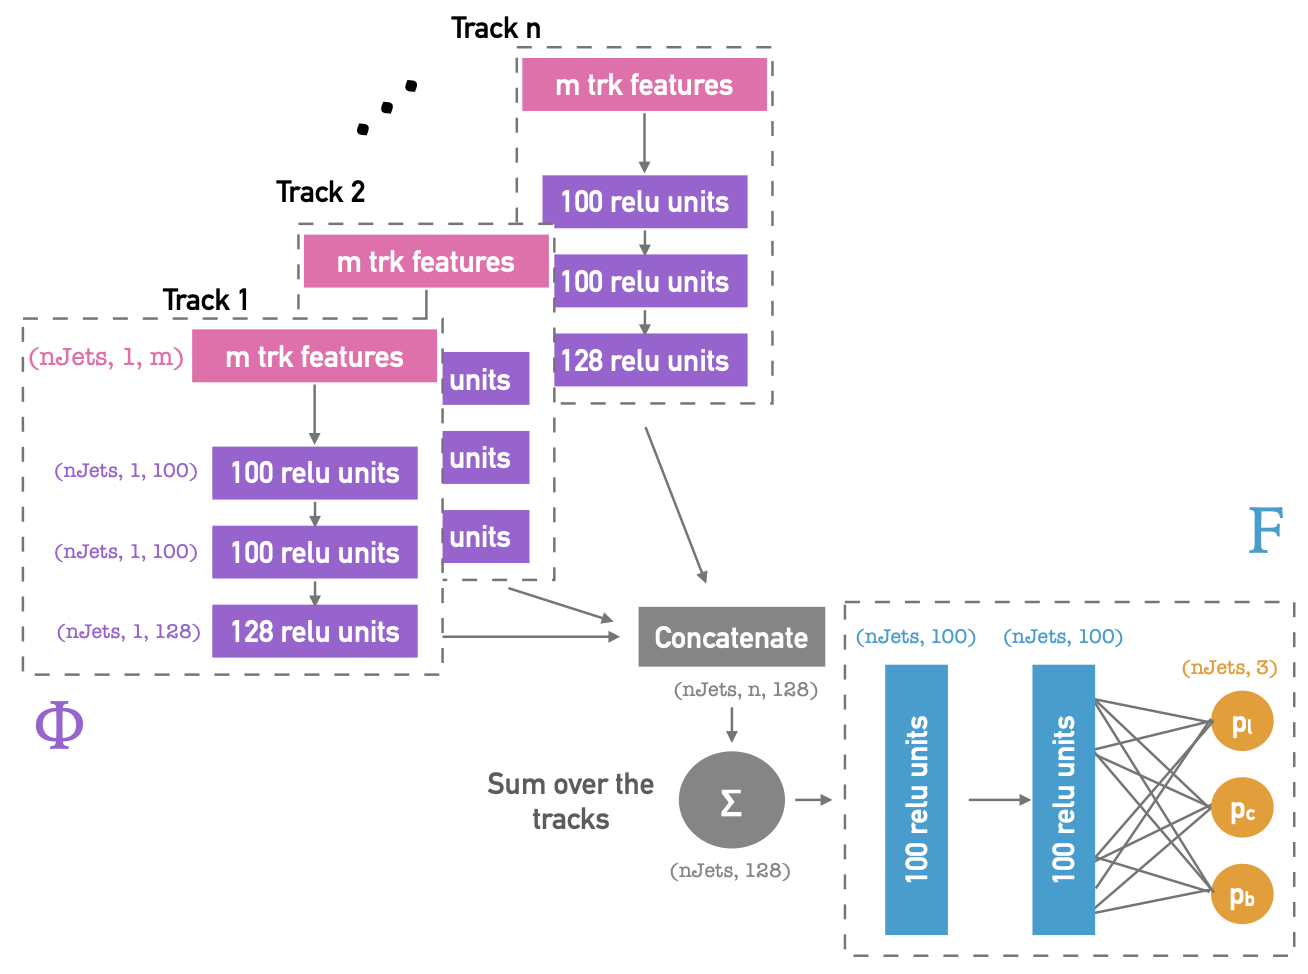
\includegraphics[scale=0.6]{Images/FTAG/dips_structure.png}
  \caption{Diagram of the \gls{dips} tagger for flavour tagging, from \cite{ATL-PHYS-PUB-2020-014}. The input consists in a set of $N$ tracks each represented by a feature vector. Each track is embedded by a \gls{dnn} track network $\Phi$ into a fixed-dimension vector. All embedded track vectors are then pooled by summation to a fixed-size vector. The last step is to process this vector with another \gls{dnn} jet network $F$ outputing the per-flavour probabilities. The number and width of layers presented here are the nominal architecture.} 
  \label{fig:dipsModel}
\end{figure}

\begin{table}[h]
  \begin{center}
      \begin{tabular}{C{3cm}|C{13cm}} 
      	 \hline \hline
          Variables & Description  \\ \hline
          $S_{d_0}$      & Lifetime signed transverse \gls{ip} significance $d_0 / \sigma_{d_0}$, with $d_0$ the transverse \gls{ip} - the transverse distance from the \gls{pv} to the point of closest approach (perigee) of the track - and $\sigma_{d_0}$ the error on $d_0$. If the perigee is in front (behind) the \gls{pv} with respect to the jet direction, the sign is positive (negative). \\ \hline
          $S_{z_0}$      & Lifetime signed longitudinal \gls{ip} significance $z_0 / \sigma_{z_0}$, with $z_0$ the longitudinal \gls{ip} - the longitudinal distance from the \gls{pv} to the perigee of the track - and $\sigma_{z_0}$ the error on $z_0$. A sign is assigned as per the prescription of $S_{d_0}$. \\ \hline
          $\log p_T^{\textrm{frac}}$   & Logarithm of the fraction of the reconstructed jet $p_T^{\textrm{jet}}$ carried by the track $\log p_T^{\textrm{frac}} = \log p_T^{\textrm{track}} / p_T^{\textrm{jet}}$. \\ \hline
          $\log \Delta R$(track, jet) & Logarithm of the geometrical distance in 2D angle between the track direction and jet axis $\log \Delta R = \log \sqrt{(\phi_{\textrm{track}} - \phi_{\textrm{jet}})^2 + (\eta_{\textrm{track} - \eta_{\textrm{jet}}})^2}$. \\ \hline
          IBL hits      & Number of hits recorded in the \gls{ibl} - 0, 1, or 2. \\ \hline
          PIX1 hits       & Number of hits in the innermost pixel layer, after the \gls{ibl} - 0, 1, or 2.  \\ \hline
          Shared IBL hits & Number of hits in the \gls{ibl} that are shared by more than one track. \\ \hline
          Split IBL hits  & Number of split hits in the \gls{ibl}, that are created by multiple charged particles. \\ \hline
          nPixHits        & Total number of hits in all the pixel layers.\\ \hline
          Shared pixel hits & Number of shared hits in the pixel layers.\\ \hline
          Split pixel hits  & Number of split hits in the pixel layers.\\ \hline
          nSCTHits          & Total number of hits in the \gls{sct} layers. \\ \hline
          Shared SCT hits   & Number of shared hits in the \gls{sct} layers.\\ \hline \hline
      \end{tabular}
      \caption{Track variables passed to the \gls{dips} model and later versions of the \gls{rnnip} model \cite{ATL-PHYS-PUB-2020-014}. Compared to the initial \gls{rnnip} variables of Table \ref{tab:rnnipVar}, the $p_T^{\textrm{frac}}$ and $\Delta R$ are passed as log values to reduce the magnitude of the long tail observed at large values and improve the training time. Shared hits are hits used by multiple tracks without being classific as split by a dedicated cluster-splitting \gls{nn} \cite{ATLAS-tracks-algo}.}
    \label{tab:dipsVar}
  \end{center}
\end{table}

This approach has several advantages over \gls{rnnip}, mainly the physically motivated permutation-invariance of the input and the improved training and evaluation time thanks to a more parallelisable architecture, as the track embedding performed by $\Phi$ can be massively parallalised on \gls{gpu}. These motivations are translated in an appreciable performance delivered by \gls{dips}, which is observed to globally outpeform version of \gls{rnnip} using the same variables, while operating at a reduced computational cost \cite{ATL-PHYS-PUB-2020-014}. The performance can be assessed from Figure \ref{fig:dipsrnnipPerf}, presenting the \gls{roc} curves for baselines trainings of \gls{dips} and \gls{rnnip} in terms of light- and $c$-rejection for $b$-jet tagging on the same held-out $t\bar{t}$ evaluation sample.

\begin{figure}[h!]
  \centering
  \begin{subfigure}[b]{0.48\textwidth}
      \centering
      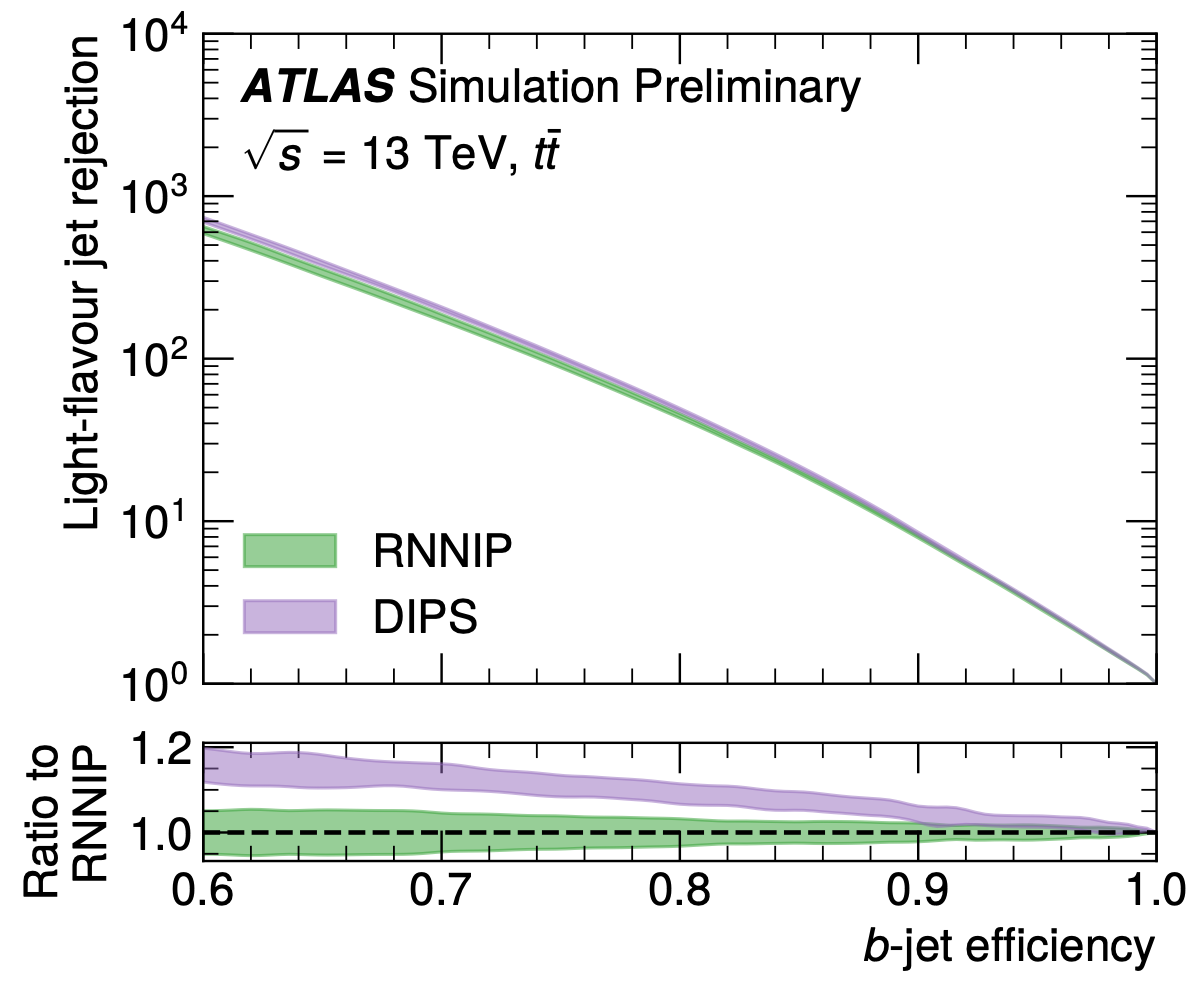
\includegraphics[width=0.98\textwidth]{Images/FTAG/dipsrnnipL.png}
      \caption{Light-rejection.} 
      \label{fig:dipsrnnipPerfL}
  \end{subfigure}
  \hfill
  \begin{subfigure}[b]{0.48\textwidth}
      \centering
      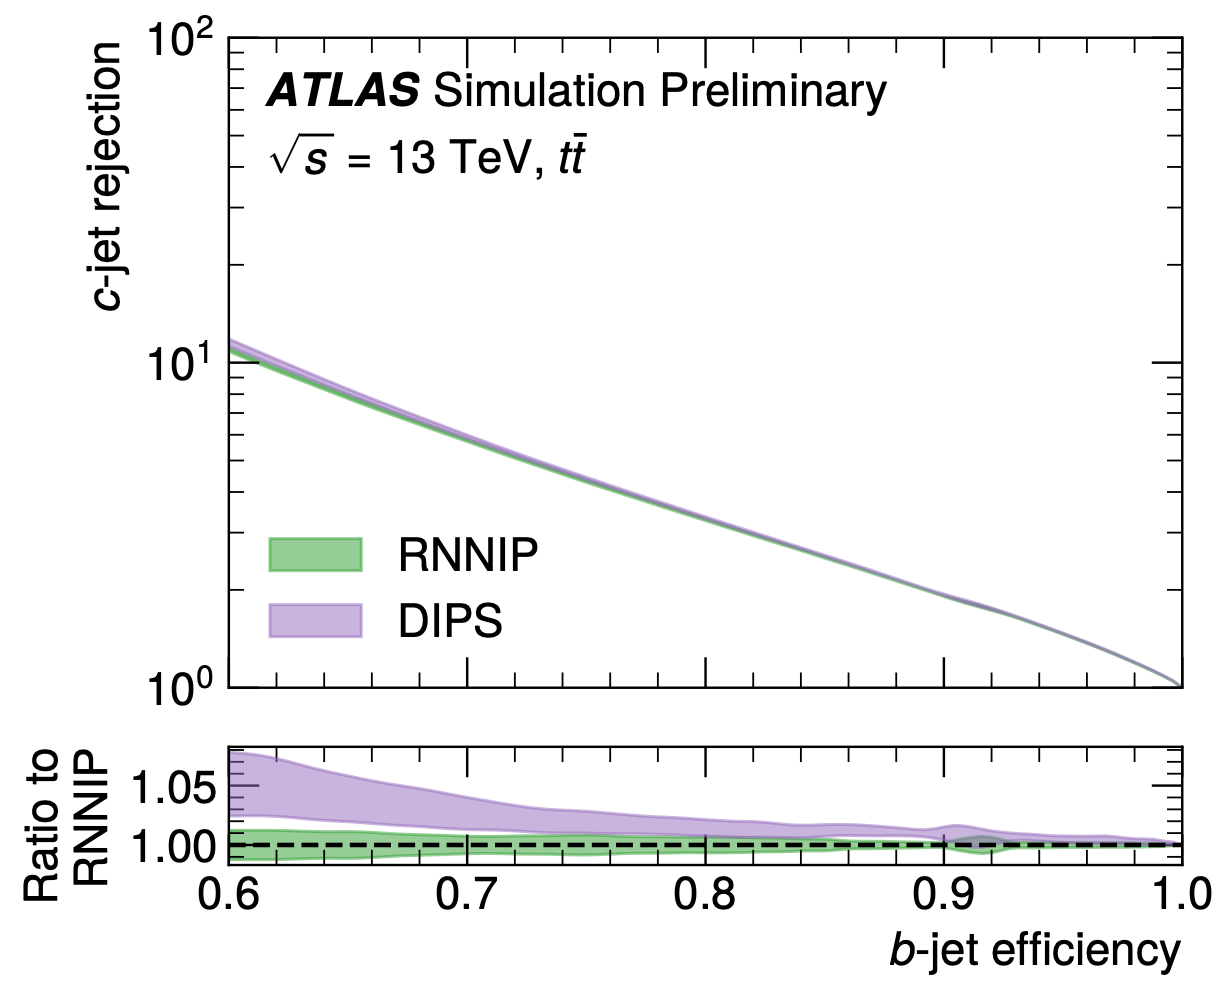
\includegraphics[width=0.98\textwidth]{Images/FTAG/dipsrnnipC.png}
      \caption{$c$-rejection.} 
      \label{fig:dipsrnnipPerfC}
  \end{subfigure}
  \caption{Light- (left) and $c$-rejection (right) as a function of $b$-jet tagging efficiency for \gls{rnnip} (green) and \gls{dips} (purple), taken from \cite{ATL-PHYS-PUB-2020-014}. Each curve and error bands show, respectively, the mean and standard deviation of the rejections for 5 trainings per algorithm. The bottom panel shows the ratio with respect to \gls{rnnip}, showing a clear performance gain for \gls{dips} at all $b$-jet efficiency considered.}
  \label{fig:dipsrnnipPerf}
\end{figure} 

The training times on the same \gls{gpu} hardware for a 48k parameters \gls{dips} model is estimated to take 78 $\pm$ 4 seconds per epoch - averaging over 5 seeds - while a 47k parameters \gls{rnnip} requires roughly thrice as much, 241 $\pm$ 14 seconds per epoch \cite{ATL-PHYS-PUB-2020-014}. The faster training time allowed the Collaboration to focus on optimisation studies of the hyperparameters. The optimisation campaign focused on three aspects of the \gls{dips} network: the architecture of the two \gls{nn}, the track selection, and the set of trac features used as input in addition to those of Table \ref{tab:dipsVar}. Regarding architecture, a grid search over various possible values for the number of layers in $\Phi$ and $F$, number of nodes, and the dimension of the track embedding space showed no significant performance change. The selected architecture is:
\begin{itemize}
  \item Track network $\Phi$: three layers of 100, 100, and 128 units applied to each track. 
  \item Jet network $F$: four layers of size 100, 100, 100, 30 before the final output of size dictated by the number of flavour to identify. 
\end{itemize}
To regularise and avoid overfitting, both batch normalisation and dropout were tested with the former observed to give better results. \\ 

The second optimisation step however uncovered that a variation to the track selection does offer opportunities for improved performance. Jets are reconstructed with the anti-kT algorithm with a radius of R = 0.4. For \gls{rnnip}, IP2D, and IP3D, the selected tracks must pass the following quality selection: $\geq$ 7 hits in the silicon layers, $\leq$ 2 missing hits in the silicon layers, $\geq$ 1 hit in the pixel detector, $\leq$ 1 hit shared by multiple tracks, $p_T$ > 1 GeV, $|d_0|$ < 1 mm, and $|z_0 \textrm{ sin}(\theta)|$ < 1.5 mm. For \gls{dips}, a looser track selection increasing the acceptance of the last three cuts was studied, modifying the nominal selection in the following way: $p_T$ > 0.5 GeV, $|d_0|$ < 3.5 mm, and $|z_0 \textrm{ sin}(\theta)|$ < 5 mm \cite{ATL-PHYS-PUB-2020-014}. Loosening the selection and keeping the top 25 tracks as ranked by decreasing $S_{d°0}$ to capture more tracks from heavy flavour decays was observed to lead to a significant improvement in performance for jets with a $p_T < 250$ GeV for \gls{dips}. From an \gls{ml} viewpoint, a larger set of input information with more noise can still prove beneficial if the underlying model is complex enough to capture useful features in the noisy data, that would otherwise be erased by a more stringent selection. The performance gain from this loosened selection-trained \gls{dips} is displayed in the \gls{roc} curves of Figure \ref{fig:dipsOptRoc}. \\

\begin{figure}[h!]
  \centering
  \begin{subfigure}[b]{0.48\textwidth}
      \centering
      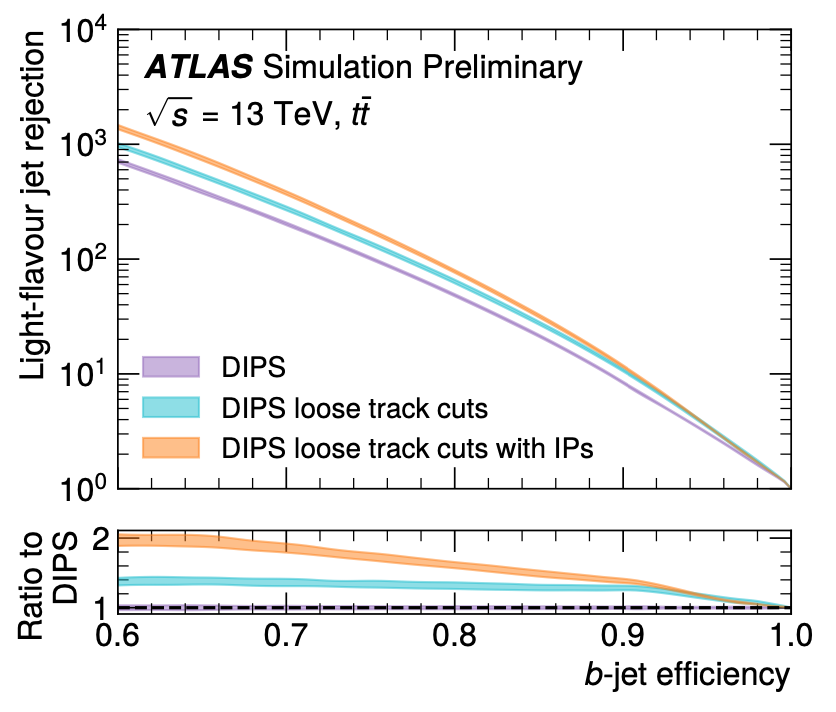
\includegraphics[width=0.98\textwidth]{Images/FTAG/dipsOptL.png}
      \caption{Light-rejection.} 
      \label{fig:dipsOptRocL}
  \end{subfigure}
  \hfill
  \begin{subfigure}[b]{0.48\textwidth}
      \centering
      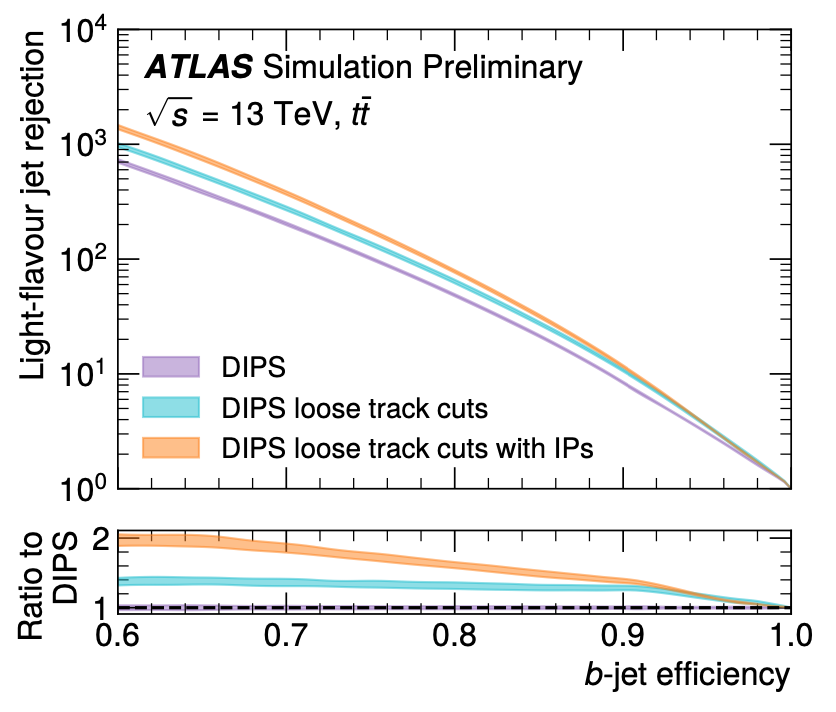
\includegraphics[width=0.98\textwidth]{Images/FTAG/dipsOptL.png}
      \caption{$c$-rejection.} 
      \label{fig:dipsOptRocC}
  \end{subfigure}
  \caption{Light- (left) and $c$-rejection (right) as a function of $b$-jet tagging efficiency for different \gls{dips} model, with the baseline (nominal) \gls{dips} in purple, the loosened track selection in blue, and the fully optimised \gls{dips} in orange, from \cite{ATL-PHYS-PUB-2020-014}. The curve and error bands show, respectively, the mean and standard deviation of the rejections for 5 trainings per algorithm with different initial random seed. The bottom panel shows the ratio with respect to the baseline \gls{dips}, showing a clear performance gain from the two steps optimisation procedure at all $b$-jet efficiency considered.}
  \label{fig:dipsOptRoc}
\end{figure} 

Furthemore, clear benefits are obtained when adding additional track features as input on top of the looser selection, as shown by the orange curve of Figure \ref{fig:dipsOptRoc}, which plots the performance of a loose track selection \gls{dips} trained with the per-track \gls{ip} parameters $d_0$ and $z_0$ in addition to the features of Table \ref{tab:dipsVar}.

\begin{figure}[h!]
  \center
  \begin{minipage}[c]{0.7\textwidth}
    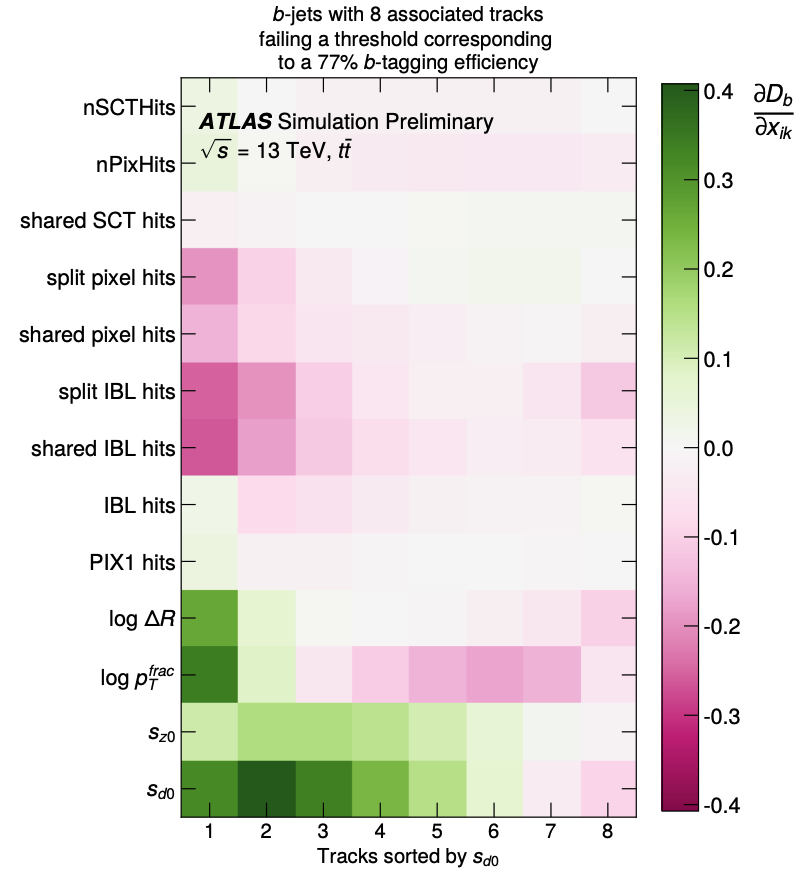
\includegraphics[width=\textwidth]{Images/FTAG/dipsSaliency.png}
  \end{minipage}
  \begin{minipage}[c]{0.25\textwidth}
    \caption{Saliency map for $b$-tagging with 8 tracks sorted by $|S_{d_0}|$, showing the gradient of the discrimant $D_b$ with respect to the track features $x_{ik}$ displayed on the $y$-axis \cite{ATL-PHYS-PUB-2020-014}.} 
  \label{fig:dipsSaliency}
  \end{minipage}
\end{figure}

How does \gls{dips} work? Interpretability of machine learning models is an active area of research. Several effective approaches exist to gauge the importance of the input on the prediction, such as Shapley values. Figure \ref{fig:dipsSaliency} presents an alternative technique called \textit{saliency maps} \cite{Simonyan2013DeepIC}. Using the $b$-tagging discriminant $D_b$ of Equation \ref{bdisc} at a fixed efficiency of 77\%, the average importance of each feature in the track inputs is assessed by averaging the gradient of the discriminant with respect to the track feature over a set of $N$ jets with strictly 8 associated tracks failing the threshold:
\begin{equation}
  \frac{\partial D_b}{\partial x_{ik}} = \frac{1}{N} \sum_{j=1}^N \frac{\partial D_b^{j}}{\partial x_{ik}^{j}},
\end{equation} 
where $i$ indexes the 8 tracks, $j$ indexes the jet in the sample of size $N$, $x_{ik}$ is the $k^{th}$ feature of the $i^{th}$ jet \cite{ATL-PHYS-PUB-2020-014}. This process effectively indicates the linear sensitivity of the discriminant on the track features. Using the saliency map, one can infer what features to modify to correct the failed tagged assigned to the $b$-jets sample. The most sensitive parameters are measured to be the \gls{ip} significances of the first five tracks, and the logarithm of the $p_T^{\textrm{frac}}$ and $\Delta R$ of the track with largest $|s_{d_0}|$. This observation is physically motivated by the dynamic of the harder fragmentation of $b$-quarks, compared to light- and $c$-quarks. Negative gradients are measured for shared and split hits observables, translating into a further incorrect discriminant under linear change of these features. This is also physically motivated, as higher count typically trace back to denser environment where random combinations of hits to form tracks are more likely. However, total hit counts in the different tracker layers have a small positive impact, as these correlate with the reconstruction of the \gls{ip} parameters.

\subsection{Training of DIPS with Variable Radius Jets for Run 3}\label{chapter:dipsVRtrain}
The physics program of the ATLAS Collaboration covers a wide range of analyses, targeting different topologies and processes at different energies. With respect to flavour tagging, a particularly relevant aspect is the energy or tranverse momenta of the jets to label. Indeed, flavour tagger are extremely sensitive to the dynamic of the underlying events. At higher energies, corresponding to higher momenta of the hadronised quark or gluon, the jet constituents emenating from the decaying parton tend to be more collimated in the same direction, as they have to share a high initial energy between themselves. This topology confends tracks and blends the rich internal jet dynamics in the measured signature, making tracks separation and secondary or tertiary vertex identification more difficult. Analyses targeting jets from hadronic or semileptonic decays of heavy particles, such as the top $t$-quark, Higgs, or the gauge bosons $W/Z$, can easily produce such highly energetic or \textit{boosted} jets.  \\

So far in this chapter, mentions of ``jets'' were always referring to the object as reconstructed by the anti-$k_T$ algorithm with a fixed radius $R = 0.4$ applied to PFLow objects, as introduced in Chapter \ref{chapter-ATLAS}. This reconstruction method proves robust in the hadron collider setting as it both leads to suitably-shaped jet structure and \gls{pu}-removing properties. This fixed radius however becomes a hurdle for boosted jet, as their average radius decreases with energy due to the collimation of the jet components. Indeed, the angular separation $\Delta R = \sqrt(\Delta\eta^2 + \Delta \phi^2)$ between the products of a decaying particle $X$ of large mass $m_X$ scales inversely to the transverse momentum \cite{ATLAS:largeRjet}: 
\begin{equation}\label{eq:sizeJet}
  \Delta R \approx \frac{2 m_X}{p_T^X}.
\end{equation}
At low $p_T^X$, the individually produced particle from the decay are sufficiently separated to be reconstructed as individual objects, hence the \textit{resolved} regime label \cite{ATLAS:2016hcf}. For example, a non-boosted Higgs decaying to a $b\bar{b}$ pair can be reconstructed as two $b$-jets with small $R$. At higher momentum however, the content of the decay is collimated and overlaps: this is the \textit{boosted} regime. The decaying particle $X$ in such a regime is typically reconstructed as a single large radius jets, to catch the different underlying jets, for example with the anti-$k_T$ method with radius $R = 1.0$. Using such a fixed large radius overestimates the size of boosted jets which are easily contaminated by the \gls{pu}, as well as the underlying event and initial-state radiations.  \\

A novel approach to model jets from boosted object decays is to reconstruct them with \gls{vr} jet algorithm \cite{vrJetPaper}, as introduced in Chapter \ref{chapter-ATLAS}. \gls{vr} jets have a size that scales with the inverse of the reconstructed jet momentum, thus correctly following the expected dynamic of Equation \ref{eq:sizeJet}. Such a significant change to the jet reconstruction is bound to have an impact on algorithms learning structure from the jet contents, as is the case of all deep learning-based taggers presented in this chapter. These models have therefore to be fine-tuned seperately to this new jet-type for optimal performance, which is the focus of this section. \\  % Chapter with VR JET

For the \gls{vr}-training, the dataset is composed of three samples simulating proton-proton collisions at $\sqrt{s} = 13$ with the following fractions:
\begin{enumerate}
  \item 85 \% of jets are sampled from the $t\bar{t}$ with a maximal $p_T$ of 400 GeV. At least one of the $W$-boson from the $t$-quark is required to decay leptonically.
  \item 7.5\% are sampled from $Z'$ events, where an exotic boson $Z'$ decays as $Z' \rightarrow q\bar{q} \textrm{ or } \tau \bar{\tau}$, with a variable $Z'$ mass to generate a flat $p_T$ spectrum extending the $p_T$-range of the jets studied up to 4 TeV. These jets are required to have a $p_T > 150$ GeV.
  \item 7.5\% are sampled from a simulated graviton process to also increase the range towards higher momenta. These jets are required to have a $p_T > 150$ GeV.
\end{enumerate}

The simulation process is similar to that introduced in Section \ref{ftagdatasets}. Figure \ref{fig:vrjetdist} displays the jet $p_T$ and $|\eta|$ distributions for the hybrid sample as well as the individual samples it is based upon, for a total of 40 $\times$ $10^6$ jets per flavour in \{$b$, $c$, light\}. In order to reach such high statistics, importance sampling is used to over-sample the limited amount of $c$-jets while using all available $b$- and downsampling light-jets. A particularity of the processing is the requirement for the $p_T$ and $|\eta|$ spectra to be equally-distributed for all jet flavours, so that these features arising from inherent physics effects in the specific processes simulated cannot be used by the model to discriminate between flavours. The technique implemented is importance sampling with replacement. It selects jets of different flavours to match a target distribution. The importance sampling weights are derived by first deriving the ratio of the target 2D distribution to the per flavour one. Weights above 1 indicate jets in the $i, j$ bin have to be oversampled, while values lower than 1 indicate the typical downsampling requirement. Jets are then iteratively sampled until the sampled distribution of each flavour individually matches the target distribution. As displayed in Figure \ref{fig:vrjetdisth} for which the target were $b$-jets, the thus constructed distribution as the same $p_T$ and $|\eta|$ distributions for all flavours. This work introduced to the first implementation of the importance sampling method, now widely used to develop flavour tagging tools.  

\begin{figure}[h!]
  \centering
  \begin{subfigure}[b]{0.98\textwidth}
      \centering
      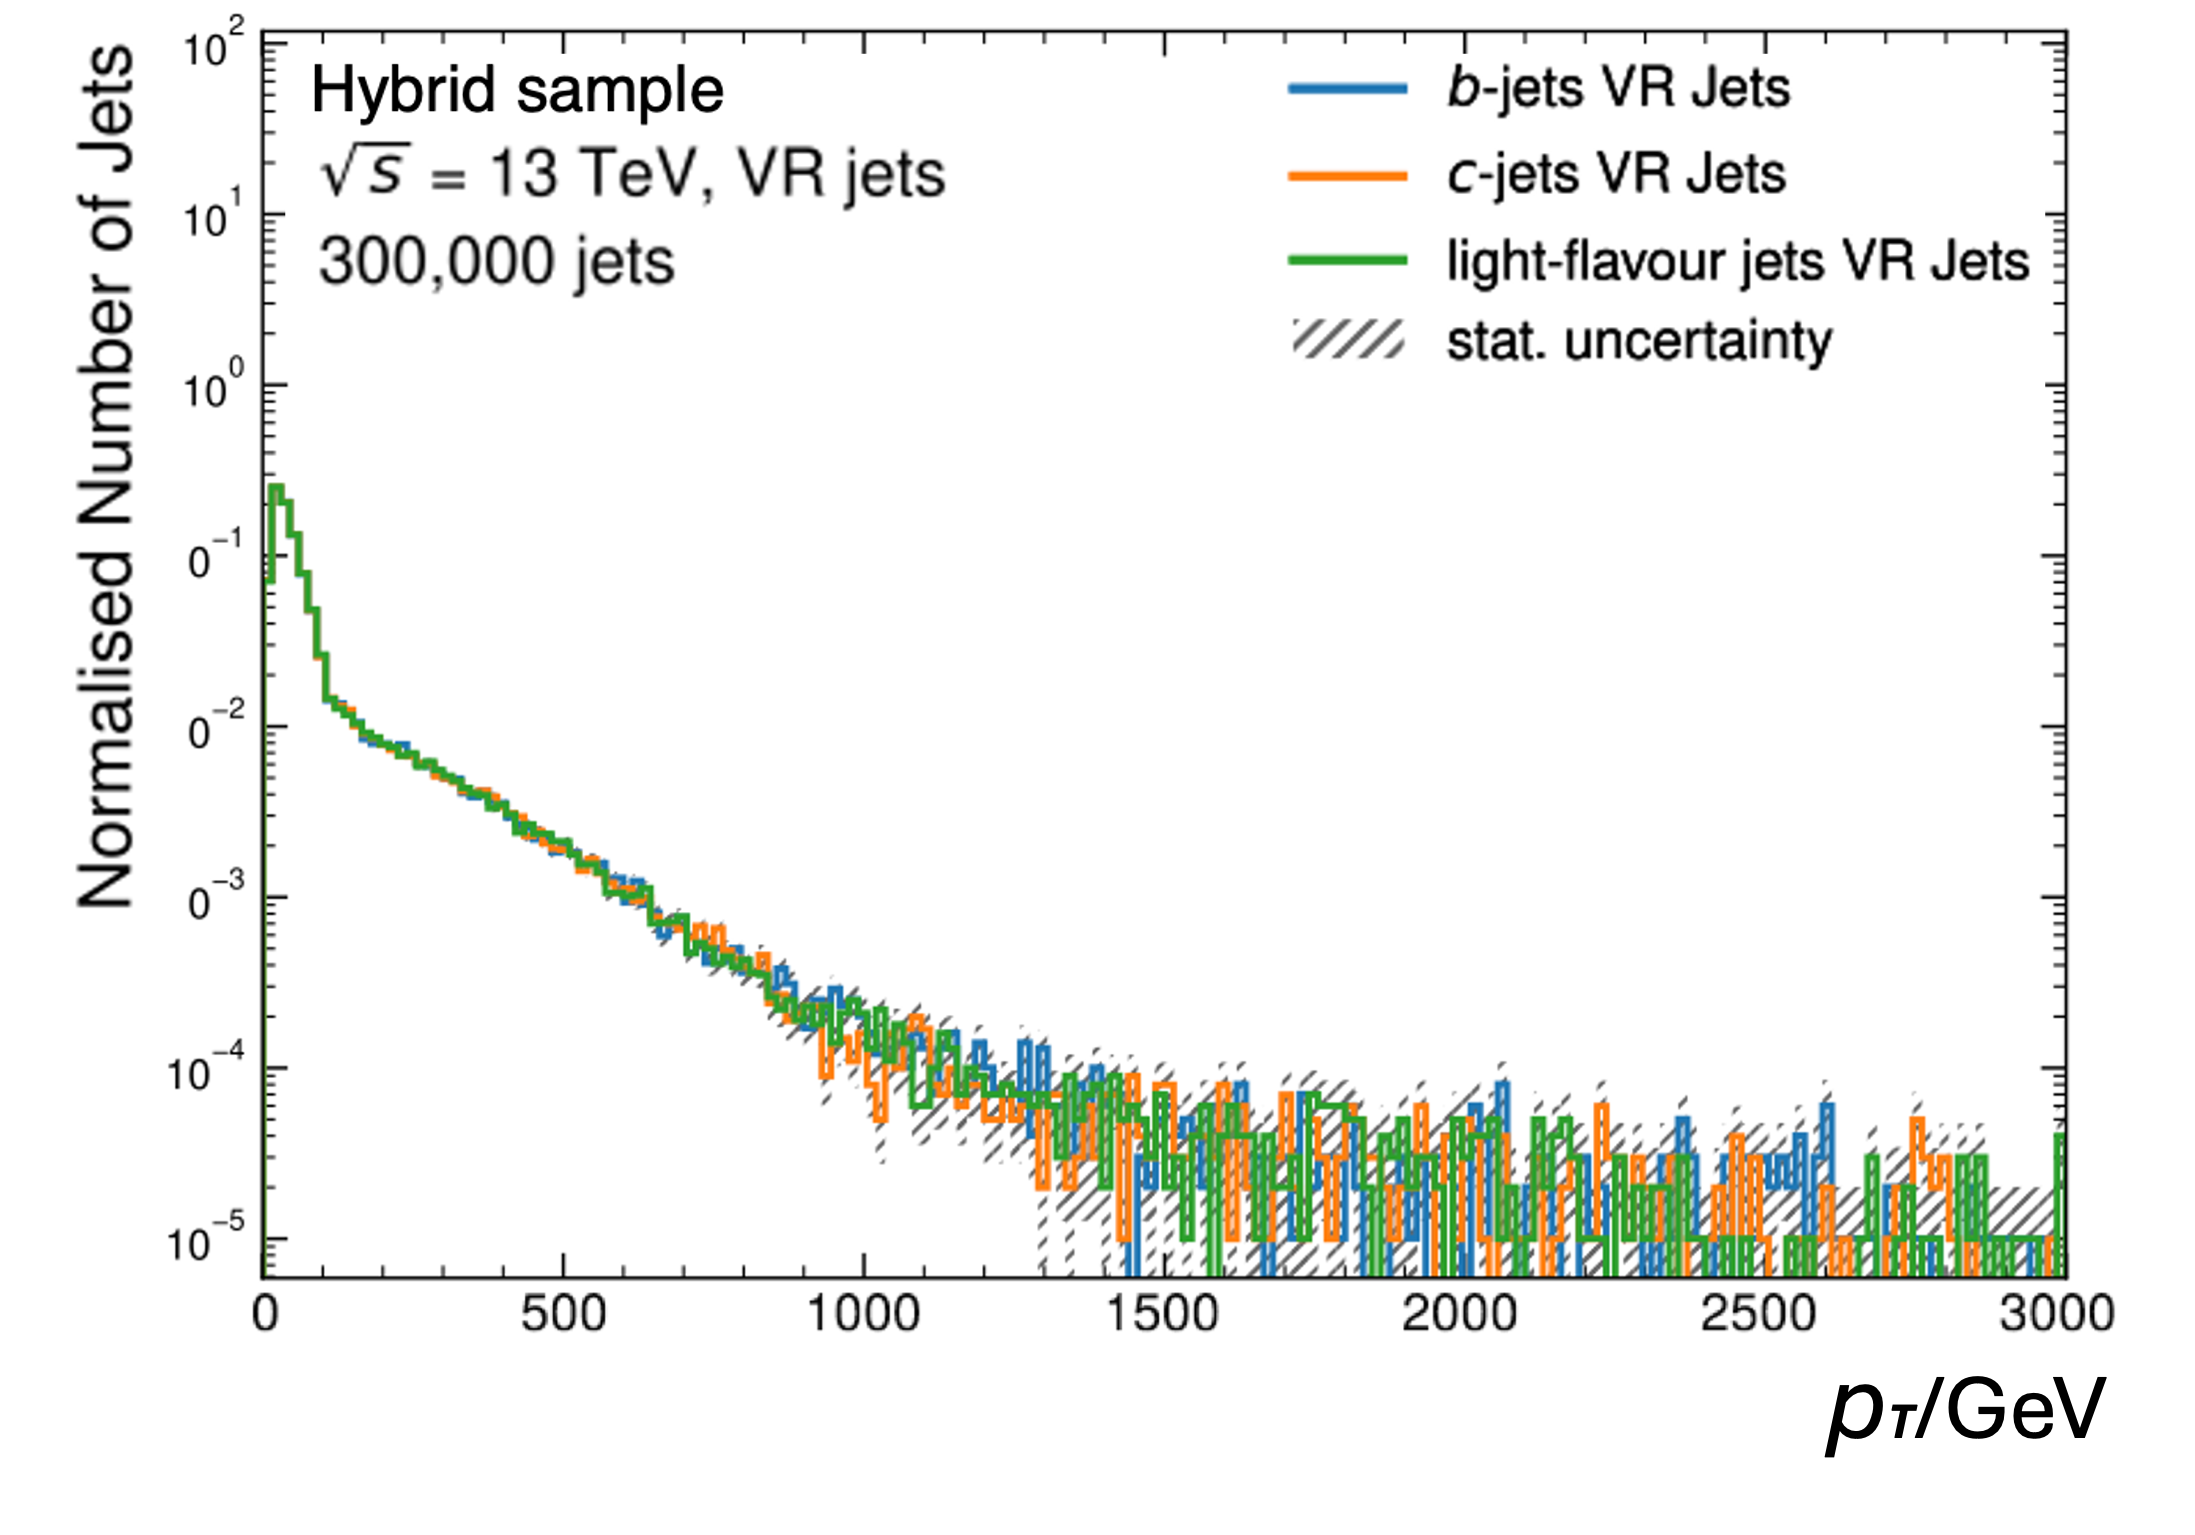
\includegraphics[width=0.48\textwidth]{Images/FTAG/VRDips/JetDist/hspt.png}
      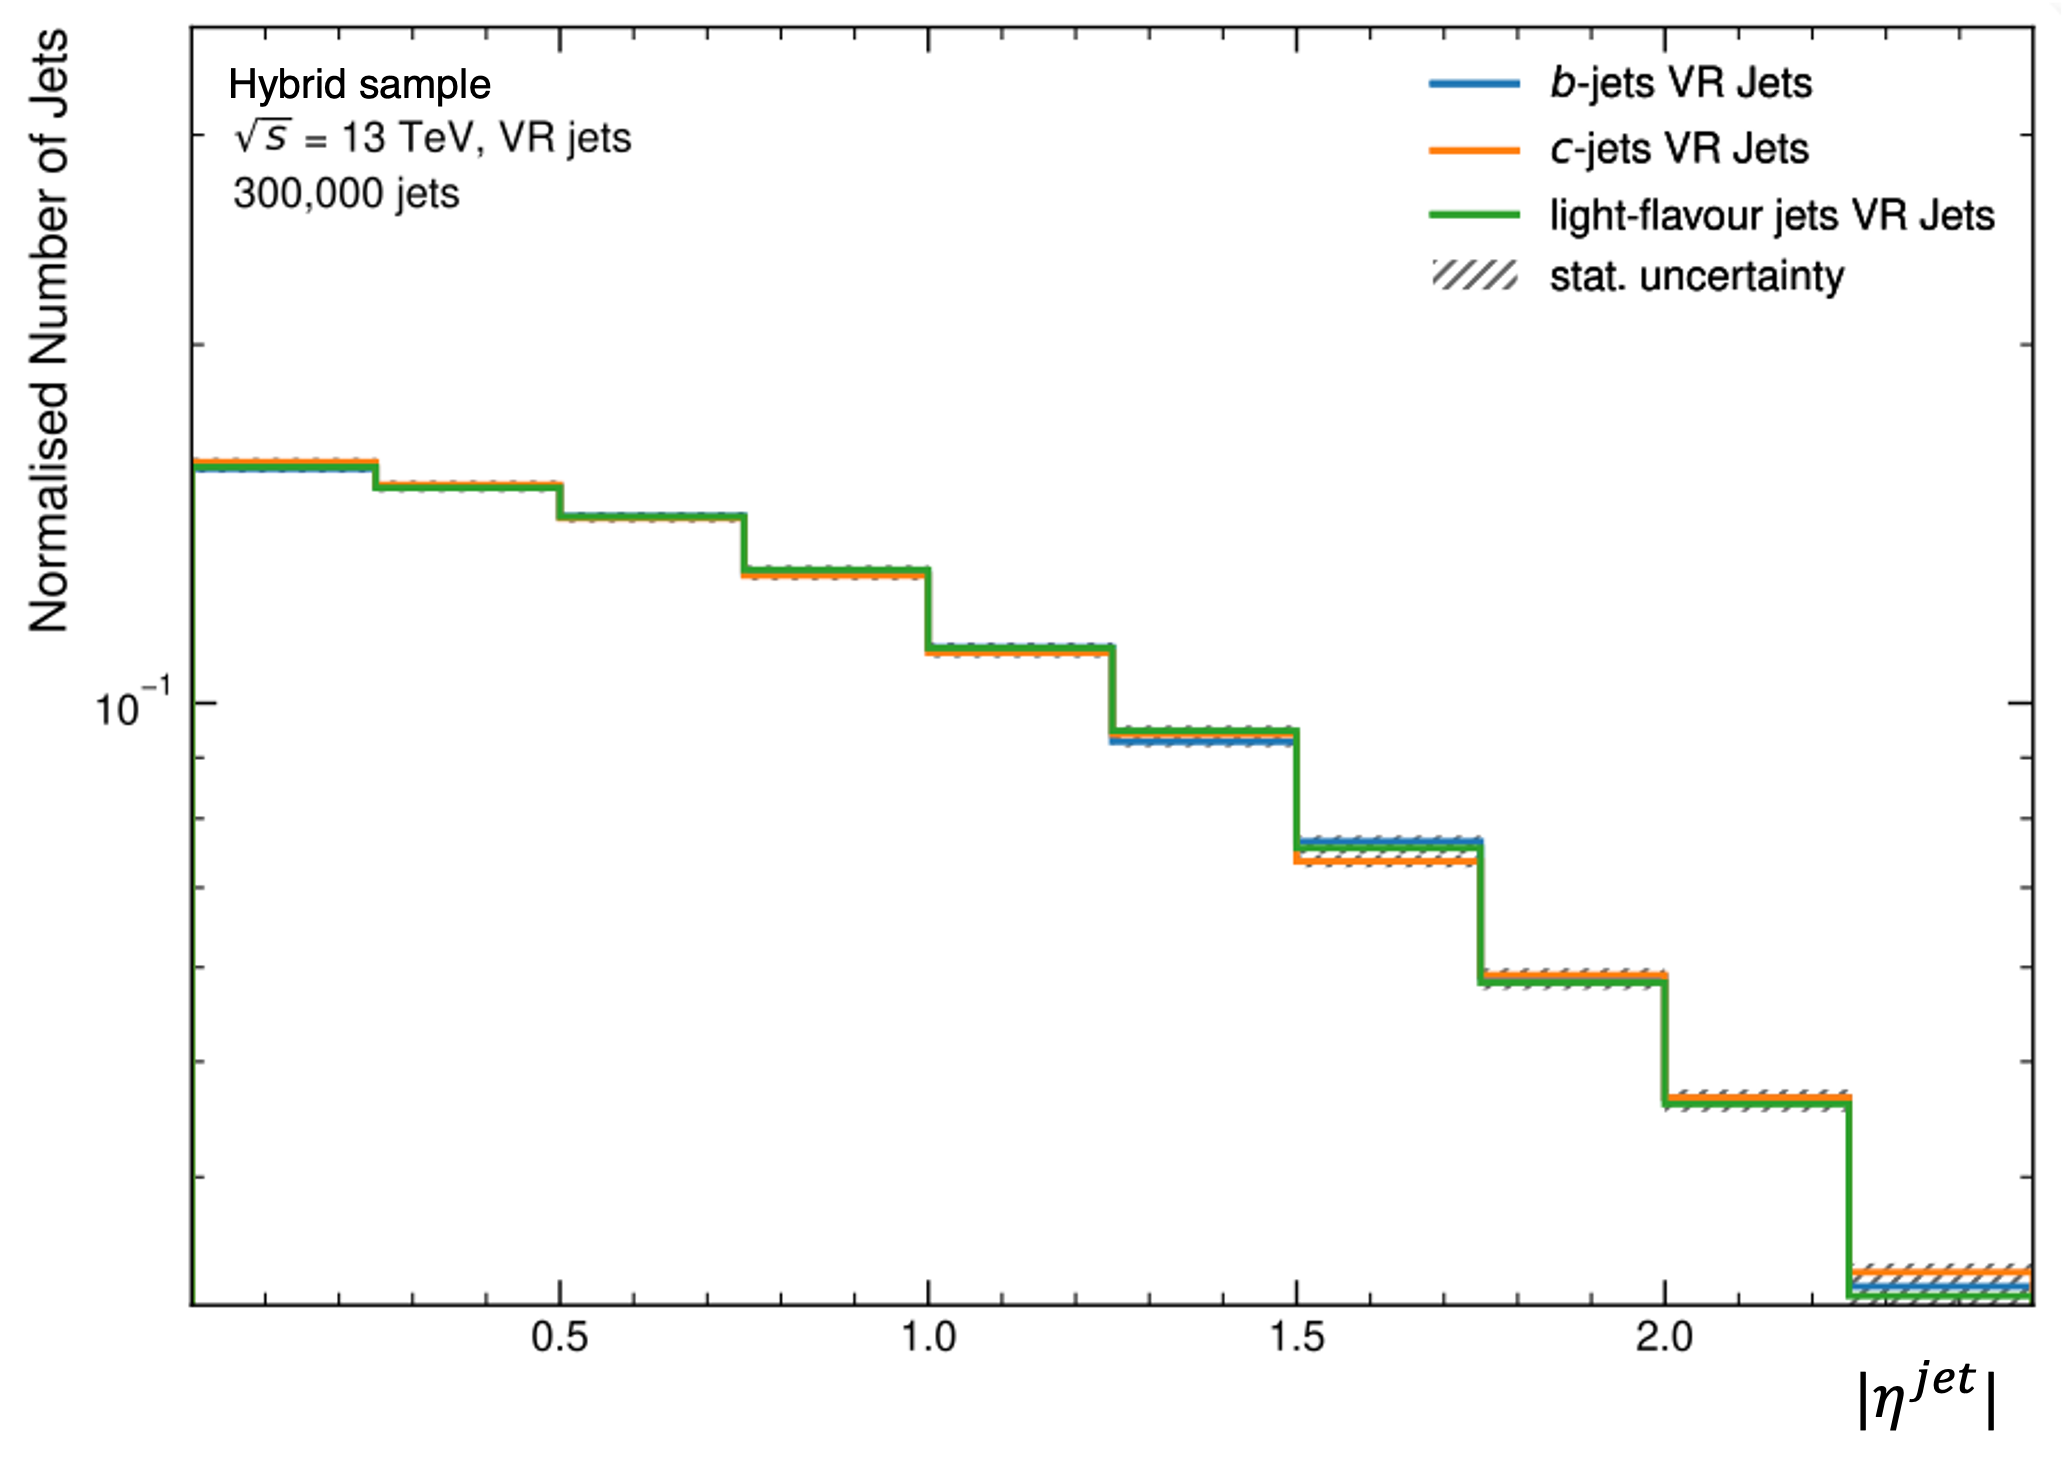
\includegraphics[width=0.48\textwidth]{Images/FTAG/VRDips/JetDist/hseta.png}
      \caption{Hybrid sample.} 
      \label{fig:vrjetdisth}
  \end{subfigure}\\
  \begin{subfigure}[b]{0.98\textwidth}
      \centering
      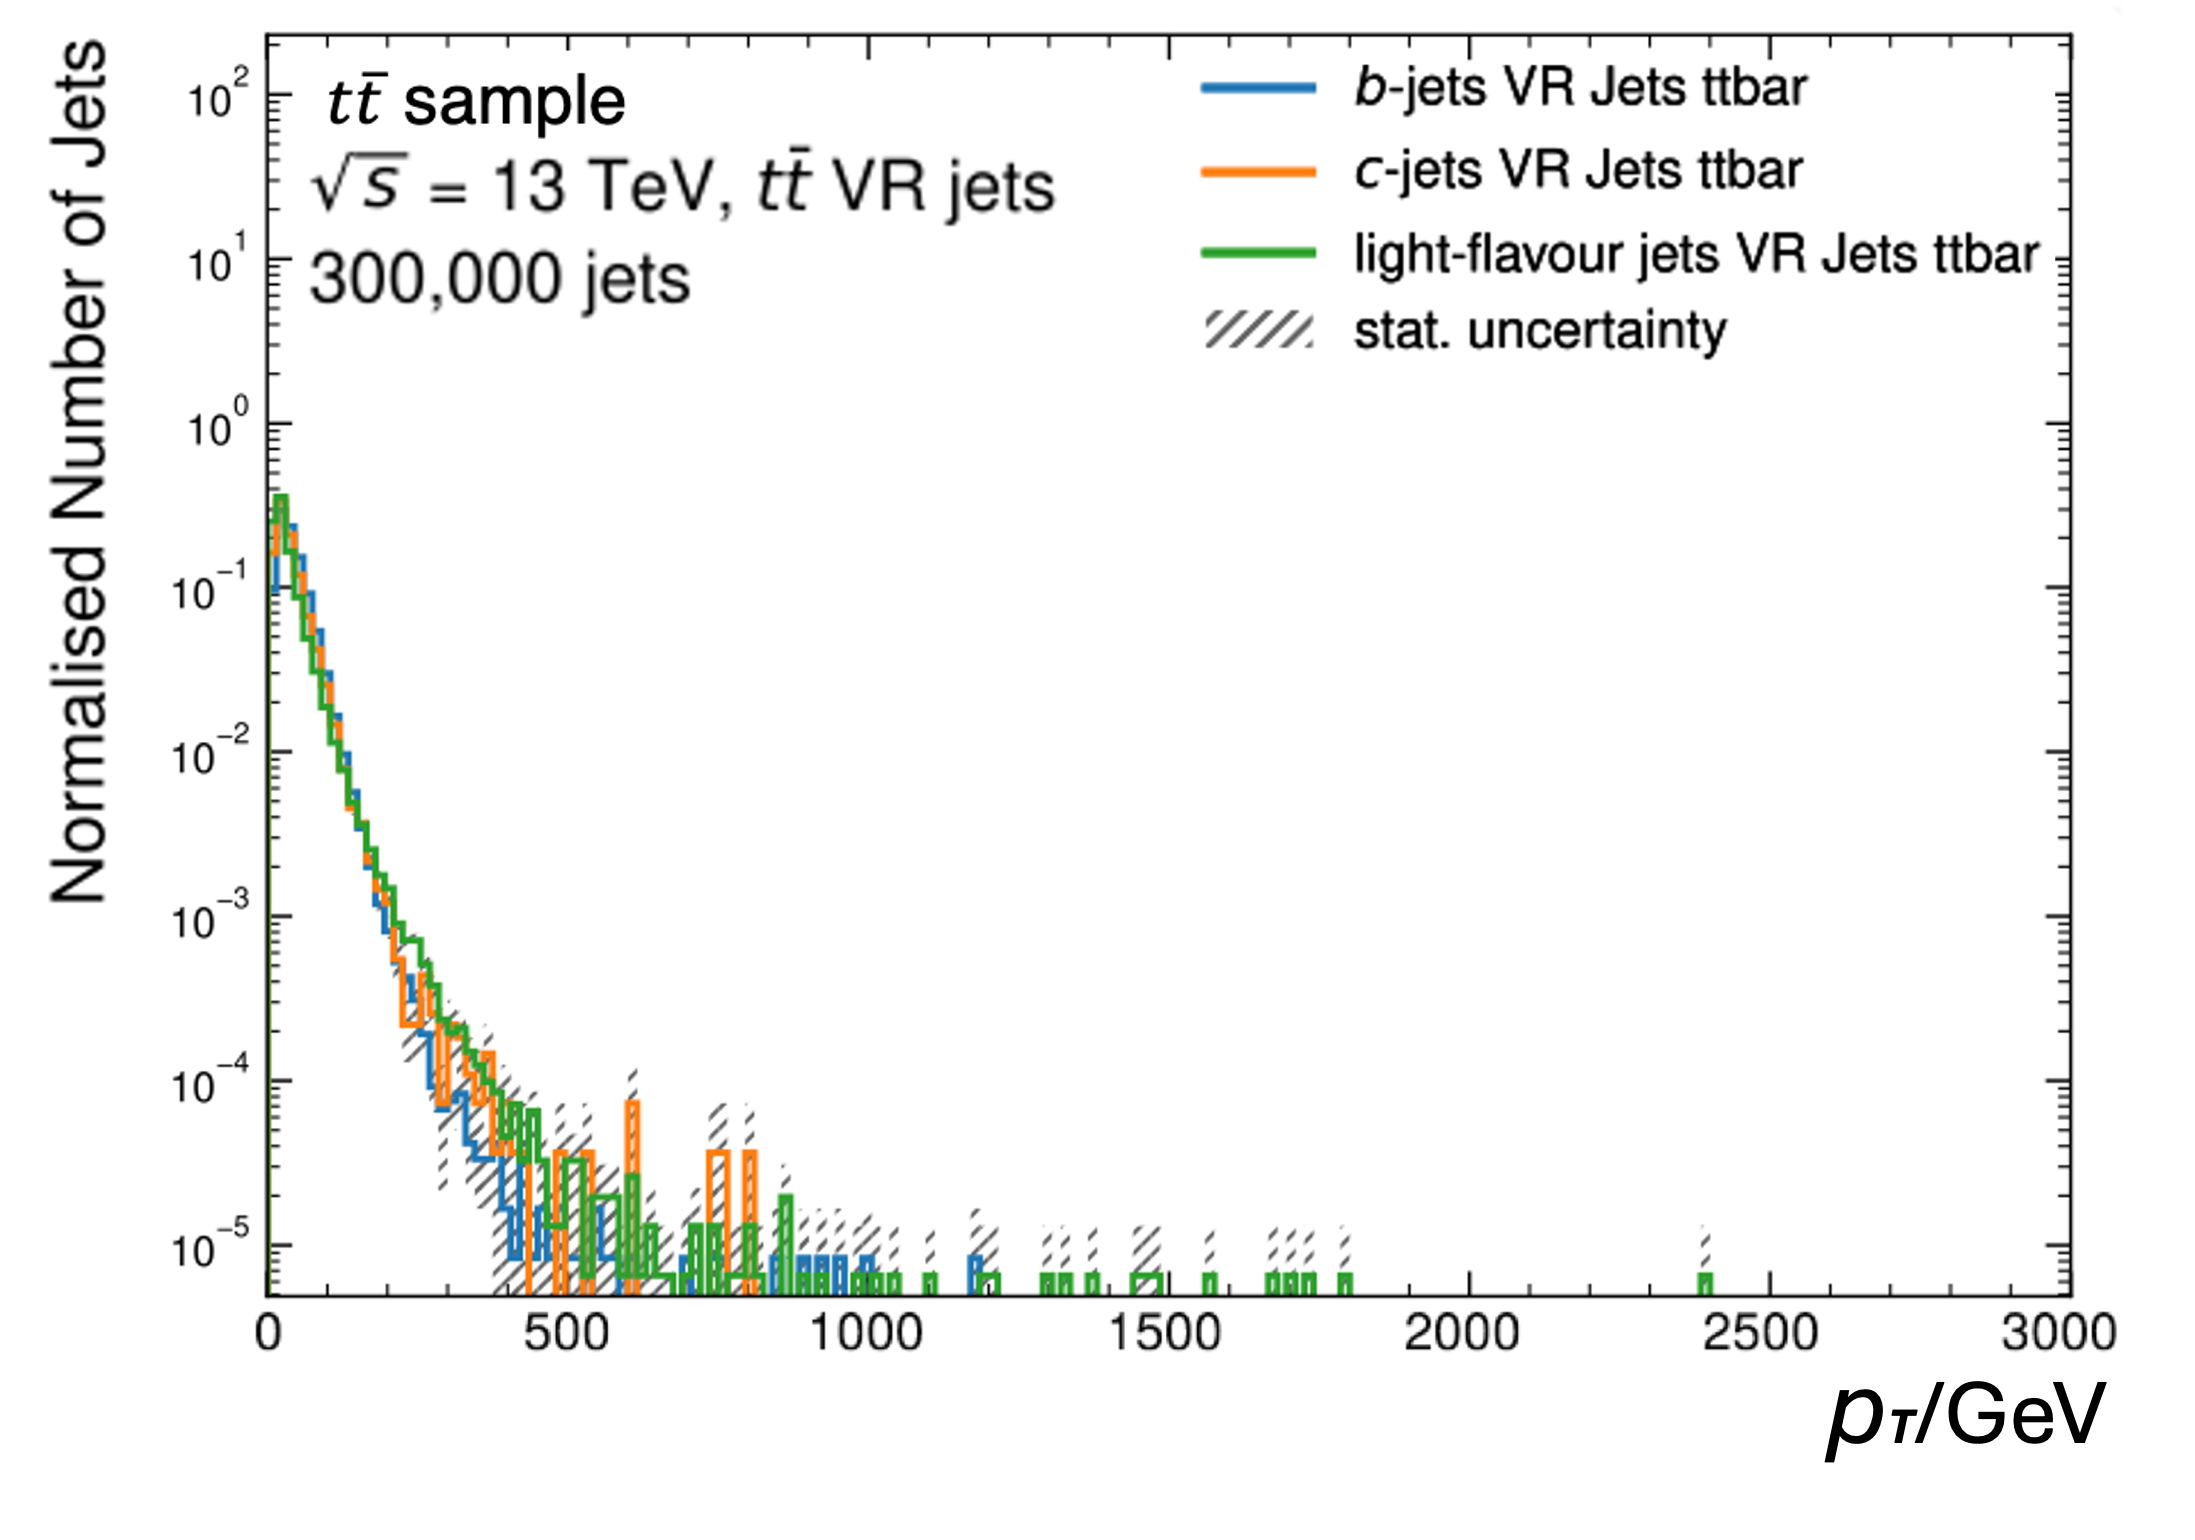
\includegraphics[width=0.48\textwidth]{Images/FTAG/VRDips/JetDist/ttpt.png}
      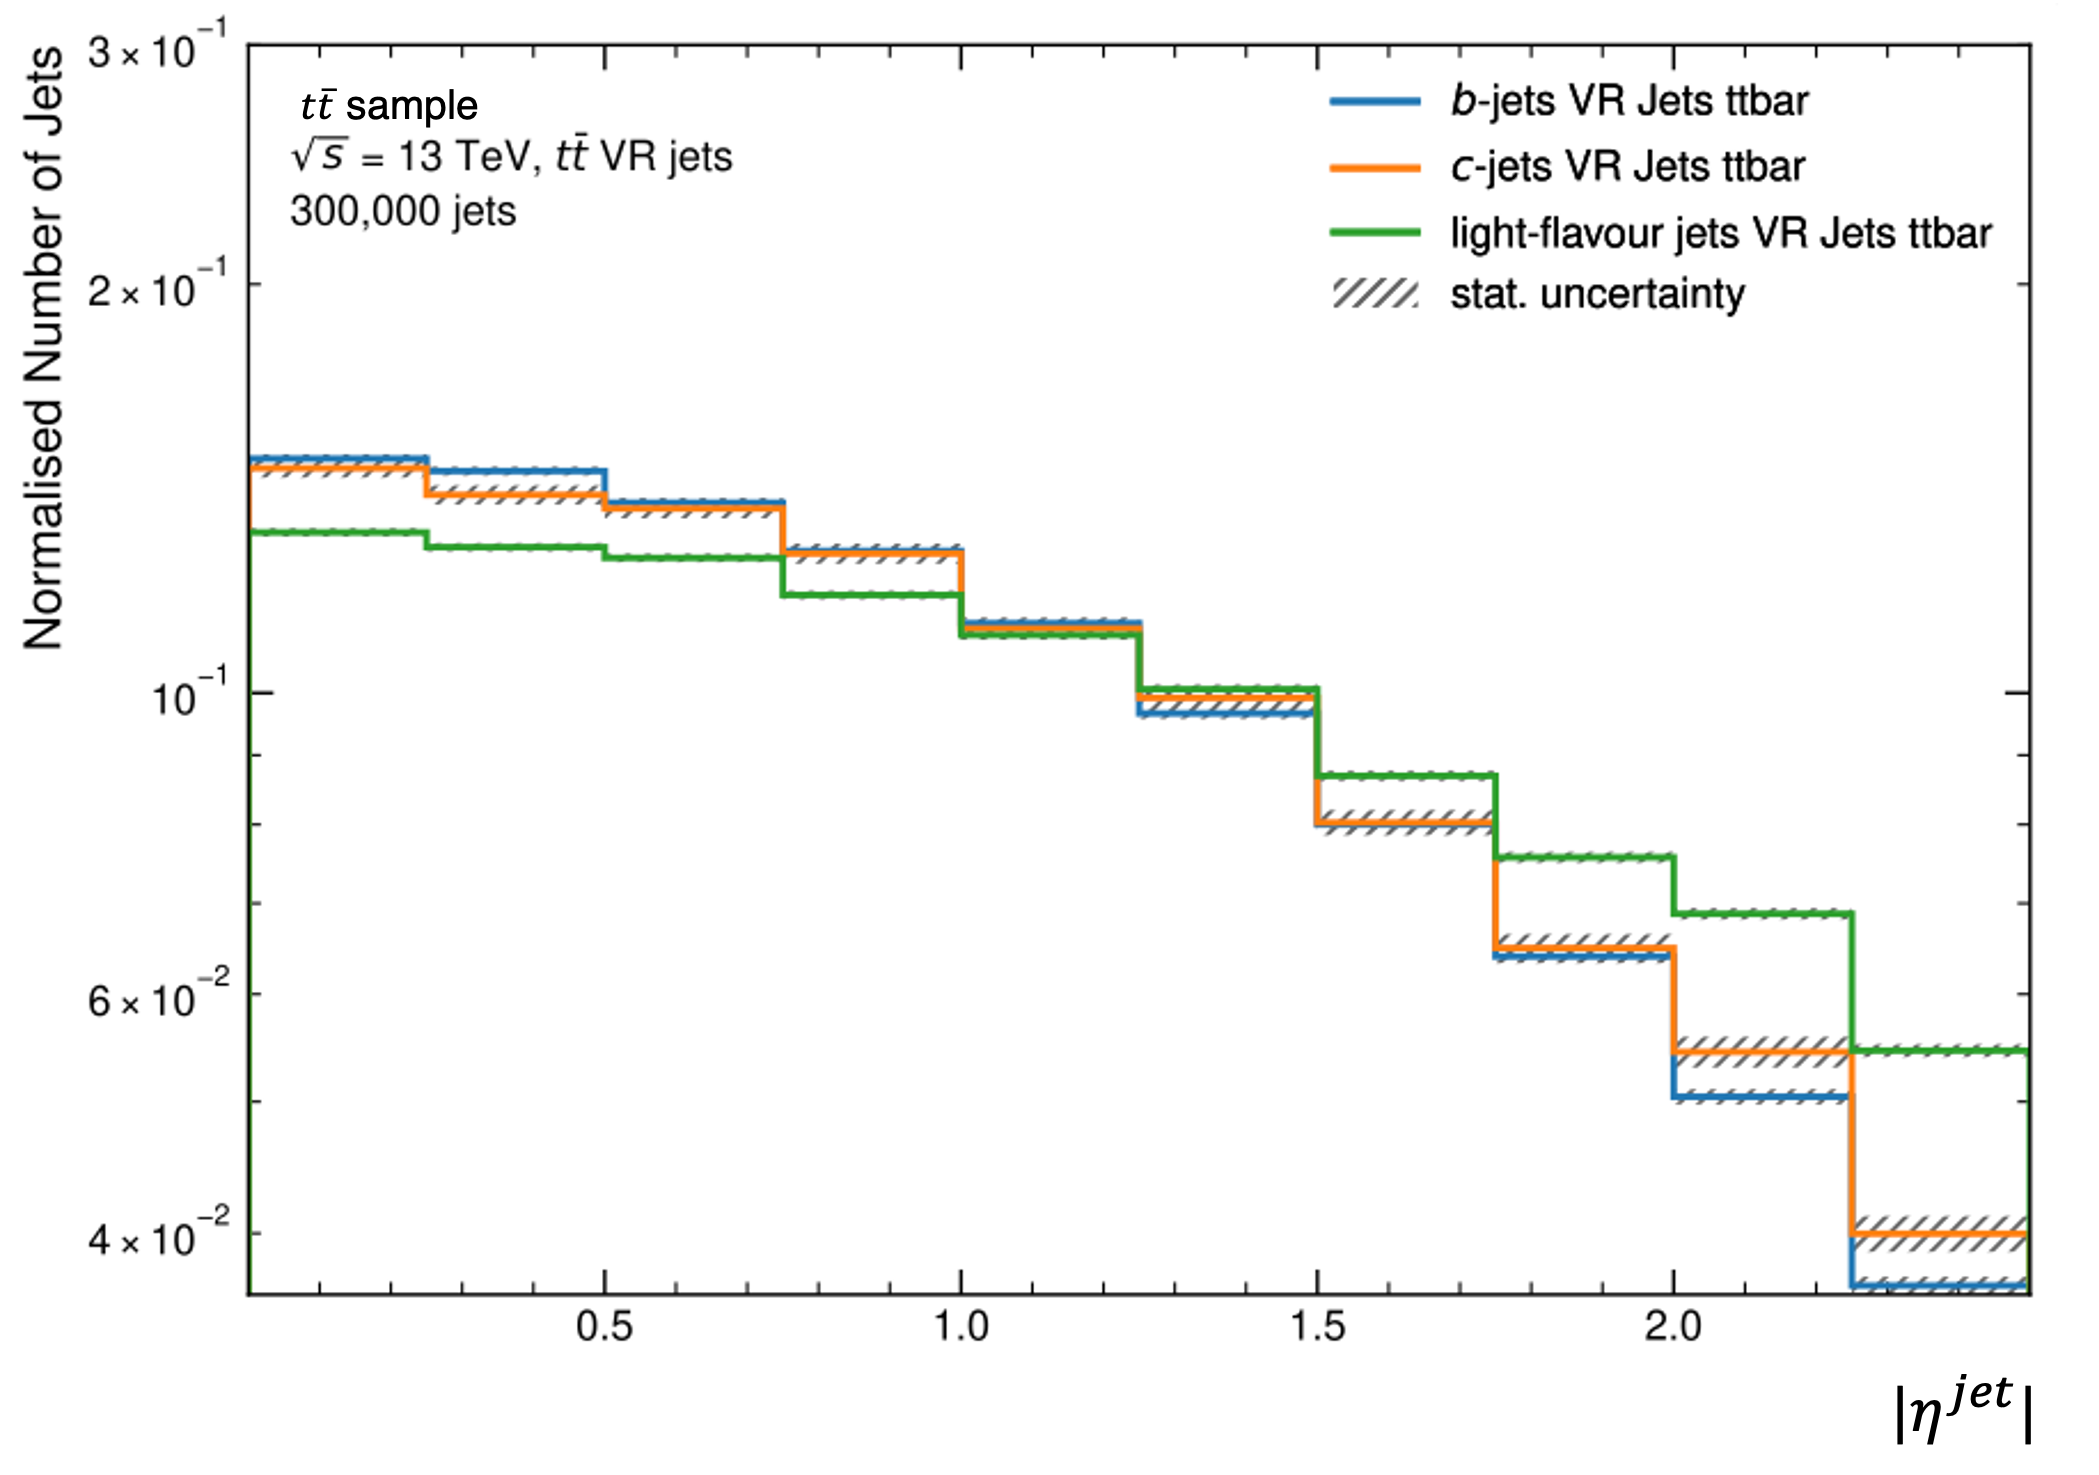
\includegraphics[width=0.48\textwidth]{Images/FTAG/VRDips/JetDist/tteta.png}
      \caption{$t\bar{t}$ sample.} 
      \label{fig:vrjetdistt}
  \end{subfigure}\\
  \begin{subfigure}[b]{0.98\textwidth}
      \centering
      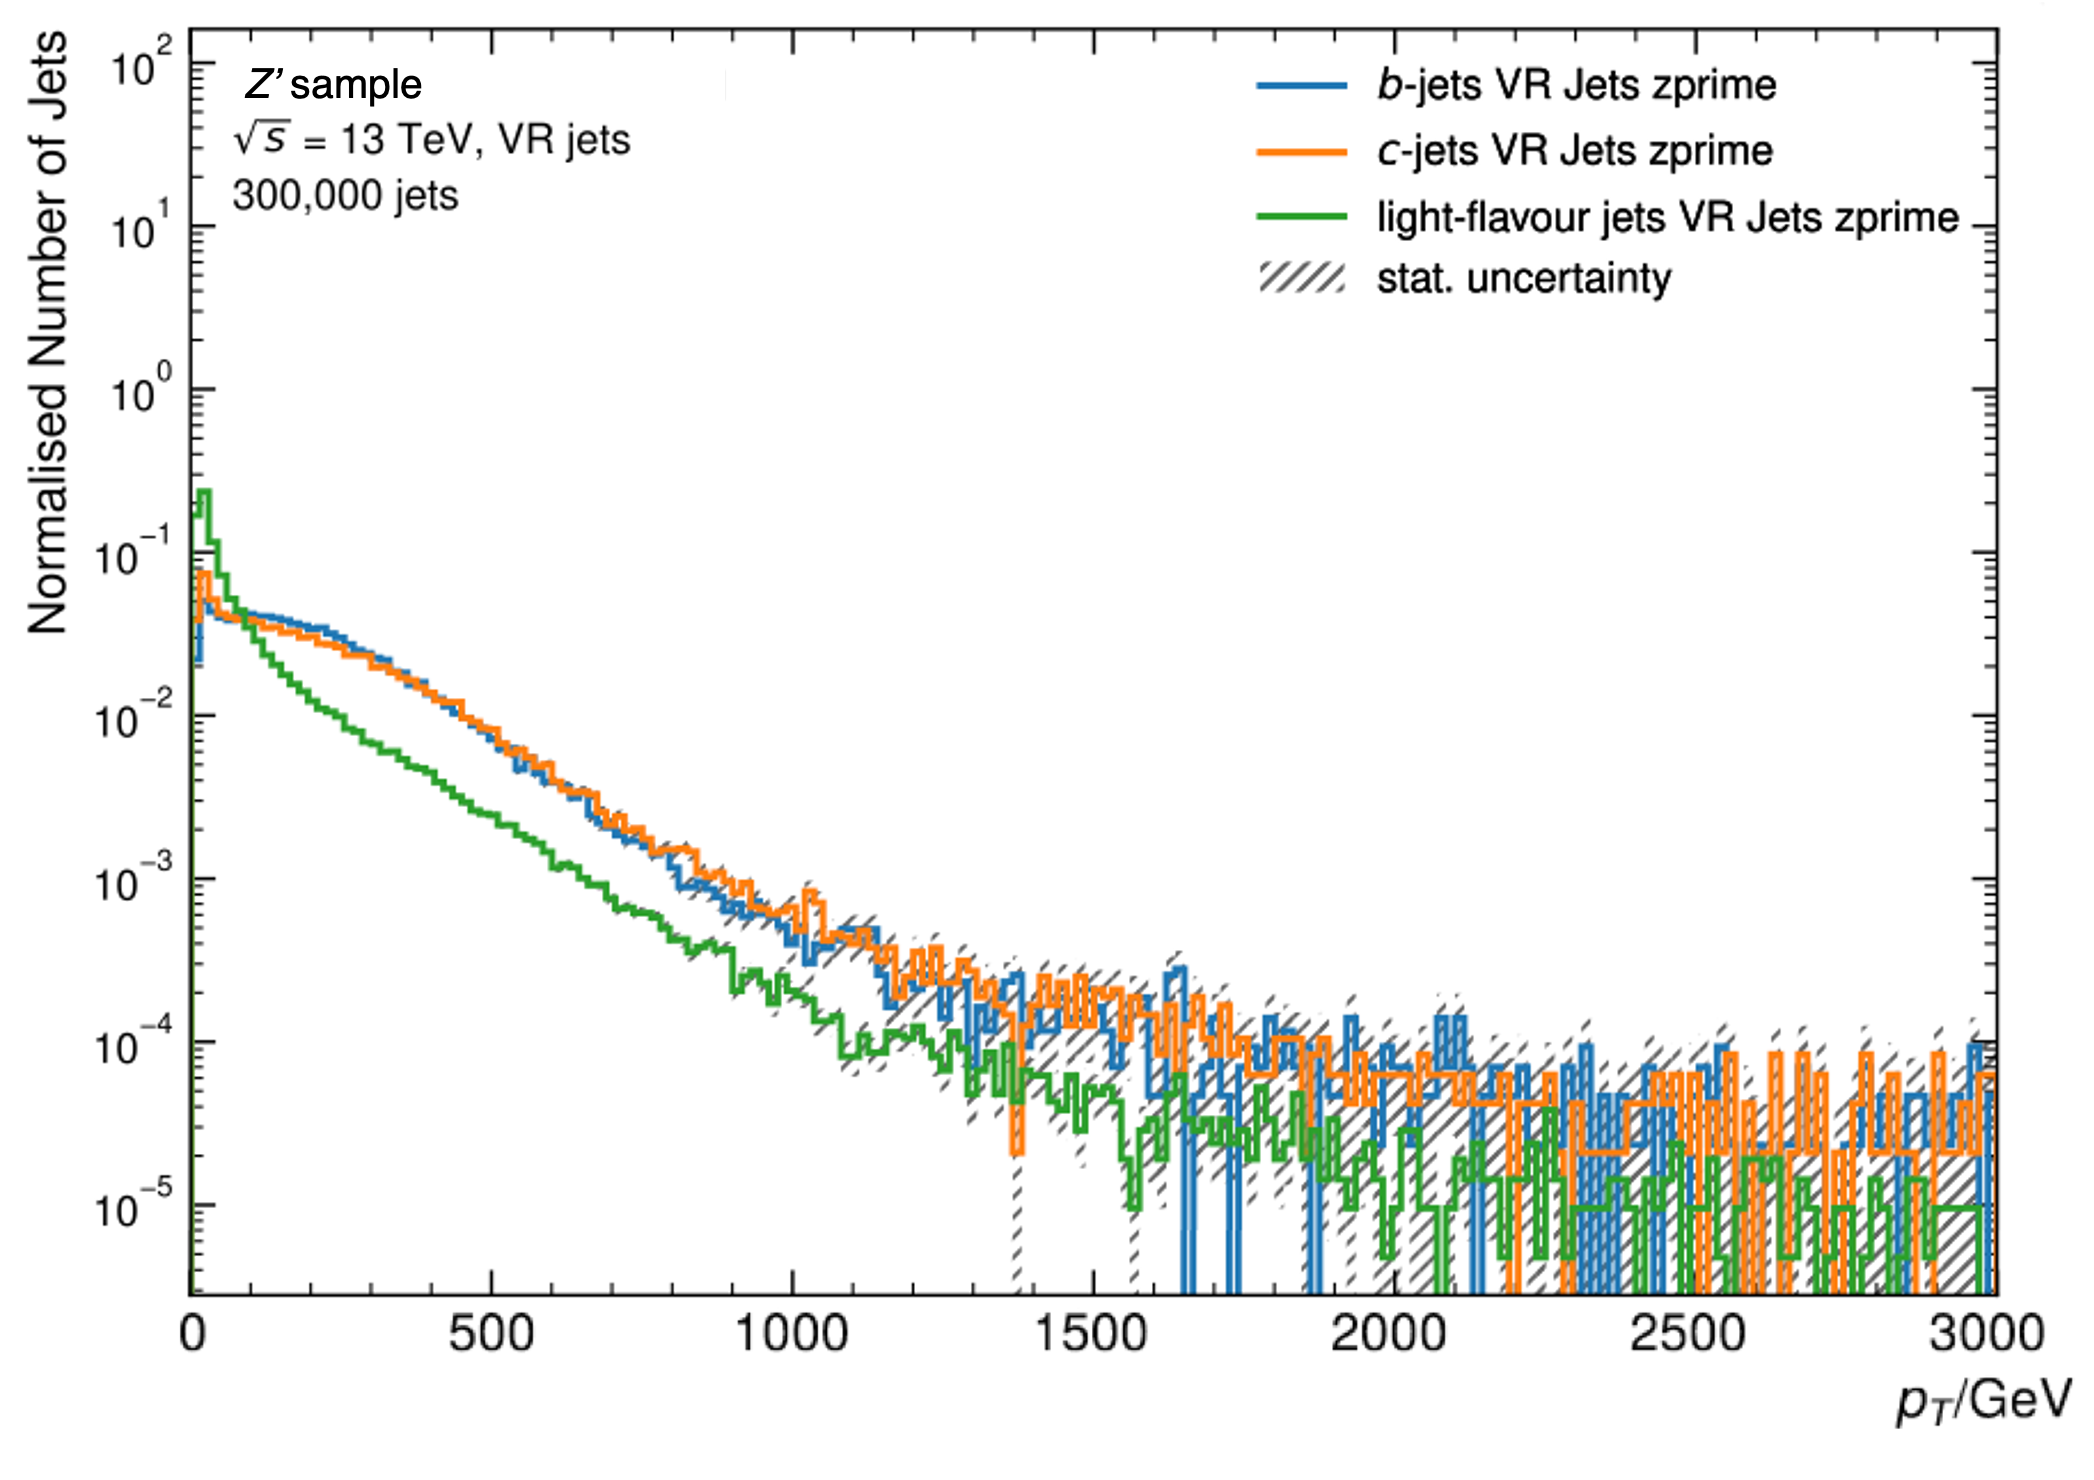
\includegraphics[width=0.48\textwidth]{Images/FTAG/VRDips/JetDist/zppt.png}
      \includegraphics[width=0.48\textwidth]{Images/FTAG/VRDips/JetDist/zpeta.png}
      \caption{$Z'$ sample.} 
      \label{fig:vrjetdiszp}
  \end{subfigure}\\
  \begin{subfigure}[b]{0.98\textwidth}
      \centering
      \includegraphics[width=0.48\textwidth]{Images/FTAG/VRDips/JetDist/grpt.png}
      \includegraphics[width=0.48\textwidth]{Images/FTAG/VRDips/JetDist/greta.png}
      \caption{Graviton sample.} 
      \label{fig:vrjetdisgr}
  \end{subfigure}
  \caption{Distributions for the \gls{vr}-jet training of jets $p_T$ (left) and $|\eta|$ (right) for the hybrid combined process (top row) made from the three bottom processes, in the order $t\bar{t}$, $Z'$, and the graviton.}
  \label{fig:vrjetdist}
\end{figure} 
 
The optimised \gls{dips} model with 62,167 learnable parameters from the previous section was trained for 200 epochs on 4 Quadro RTX 8000 \gls{gpu}. The learning rate started at 0.001 and was reduced by a factor 0.8 on plateaus of 3 epochs, with a batch size of 15k jets, batch normalisation, and a dropout rate of 0.1 for the $F$ network. Training proved stable with no signs of overtraining. The model at the epoch giving the smallest loss on a heldout validation set of 300k jets as well as the best light- and $c$-rejections at a fixed 77\% $b$-tagging efficiency was selected for further comparison. Figure \ref{fig:dipsVRROC} shows the \gls{roc} curves for $b$- and $c$-tagging of the best \gls{dips} model on \gls{vr}-jets (blue), as well as some comparison to the \gls{dips} model trained on PFlow jets (orange) and \gls{rnnip} trained on \gls{vr}-jets from the previous software release R21 (green). 

\begin{sidewaysfigure}
  \vspace{0.5cm}
  %\hspace{0.5cm}
  \begin{subfigure}[t]{0.3\textwidth}
    \centering
    \includegraphics[scale=0.43]{Images/FTAG/VRDips/ROC/ttb.png}
    \caption{$t\bar{t}$ test sample $b$-tagging.}
    \label{fig:dipsVRROCtt}
  \end{subfigure}
  \hfill
  \begin{subfigure}[t]{0.3\textwidth}
    \centering
    \includegraphics[scale=0.43]{Images/FTAG/VRDips/ROC/zpb.png}
    \caption{$Z'$ test sample $b$-tagging.}
    \label{fig:dipsVRROCzp}
  \end{subfigure}
  \hfill
  \begin{subfigure}[t]{0.3\textwidth}
    \centering
    \includegraphics[scale=0.43]{Images/FTAG/VRDips/ROC/grb.png}
    \caption{Graviton test sample $b$-tagging.}
    \label{fig:dipsVRROCgr}
  \end{subfigure} \\
  \begin{subfigure}[t]{0.3\textwidth}
    \centering
    \includegraphics[scale=0.43]{Images/FTAG/VRDips/ROC/ttc.png}
    \caption{$t\bar{t}$ test sample $c$-tagging.}
    \label{fig:dipsVRROCttc}
  \end{subfigure}
  \hfill
  \begin{subfigure}[t]{0.3\textwidth}
    \centering
    \includegraphics[scale=0.43]{Images/FTAG/VRDips/ROC/zpc.png}
    \caption{$Z'$ test sample $c$-tagging.}
    \label{fig:dipsVRROCzpc}
  \end{subfigure}
  \hfill
  \begin{subfigure}[t]{0.3\textwidth}
    \centering
    \includegraphics[scale=0.43]{Images/FTAG/VRDips/ROC/grc.png}
    \caption{Graviton test sample $c$-tagging.}
    \label{fig:dipsVRROCgrc}
  \end{subfigure}
  \caption{\gls{roc} curves for $b$-tagging (top) and $c$-tagging (bottom) on test samples of 300 k jets for $t\bar{t}$ (left), $Z'$ (centre), and the graviton process (right). Models are displayed as curves of different colours, with the \gls{vr}-jets \gls{dips} in blue, the \gls{dips} model trained on PFlow jets in orange, and \gls{rnnip} trained on \gls{vr}-jets from the previous software release R21 in green.}
  \label{fig:dipsVRROC}
\end{sidewaysfigure}

Training \gls{dips} on a dedicated set of \gls{vr}-jets clearly improves performance over relying on the PFlow-trained version, as observed by comparing the blue (\gls{vr}-trained \gls{dips}) to orange curves (PFlow-trained \gls{dips}). At a $b$-tagging efficiency of 77\%, the light-rejection is PFlow-trained \gls{dips} is indeed roughly 40\% lower. However, the $c$-rejection does not benefit as much, being either on par or even lower for the \gls{vr}-trained \gls{dips} on the $t\bar{t}$ samples. This difference in performance indicates an inappropriate choice of $f_c$ value for the $b$-tagging discriminant of the \gls{vr}-trained \gls{dips}. A so-called \textit{flavour fraction scans}, displaying the rejections at a fixed tagging efficiency for different value of the flavour fraction, can lead to a better choice for a balanced improvement in both background jet rejections. However, \gls{dips} probabilities are not meant to be used directly as discrimant but rather passed on to the high level algorithm \gls{dl1d}, hence this optimisation is reserved for the final model as presented in Chapter \ref{sec:VRdl1dTrain}. Figures \ref{fig:dipsVRROCttc} to \ref{fig:dipsVRROCgrc} lead to similar conclusions for $c$-tagging.

\subsection{Training of DL1d \& DL1r with PFlow for Run 3}
The ATLAS Collaboration continuously updates its software, updating specific methods to adopt new techniques, maintaining its many tools and adding capabilities. In preparation for the current Run 3 of the \gls{lhc} that started in 2022, ATLAS improved its reconstruction software from release 21 (R21) to release 22 (R22). As such, important elements used by flavour tagging methods have changed, requiring to retrain all taggers to ensure optimal performance under the new conditions. This work presents the first ATLAS study of the retraining of \gls{dl1r} on the new release R22 and the first training of \gls{dl1d}, including the \gls{dips} sub-tagger in the high-level flavour tagging tool. Other important novelties of this work are the possible inclusion of $\tau$-jets in the \gls{dl1} model's predictions and a new technique to efficiently process the training data into high statistics dataset using importance sampling, as mentioned in the previous section. The interest of including $\tau$ stems from their tendency to be miss-classified as $c$-jets when hadronically decaying, as both particles commonly leave three particles in the detector. The resulting taggers are observed to efficiently identify $\tau$-jets thereby providing a new way to perform $\tau$-identification and improving $c$-jet tagging. However, due to the widespread use of the \gls{ftag} algorithms and the difficulties arising in calibrating a tagger with excellent rejection against $\tau$-jets, these are not included in the default version of the tagger nor in the results shown here, but are actively under study for the new generation of tagger in the GN family. \\ % Problem: reference to tau tagging but no plots ... add them?
Two samples, the $t\bar{t}$ and $Z'$ from proton-proton collisions at $\sqrt{s} = 13$, are simulated and combined in the datasets, as described in Section \ref{ftagdatasets}. For both samples, PFlow jets are reconstructed using the anti-$k_T$ algorithm with radius $R = 0.4$. These two samples are combined into a single \textit{hybrid} sample to train the taggers, with 70\% of the total number of jets coming from $t\bar{t}$ and the remaining from the $Z'$. The $t\bar{t}$ and $Z'$ samples cover, respectively, a low- and high-$p_T$ region based on a reconstructed $b$-hadron $p_T$ separation threshold of 250 GeV for $b$-jets and a jet $p_T$ of 250 GeV for non-$b$-jets. They are re-sampled to have the same $p_T-|\eta|$ distributions, as described in the next paragraph. The relative proportion of each sample was chosen to avoid any discontinuity in the $p_T$ spectrum at their junction, as evidenced in Figure \ref{fig:distTraining}. The final evaluation of the performance of a trained tagger is performed on separated test sets of both processes and unfolded over the flavours.\\

\begin{figure}[h!]
  \center
  \includegraphics[width=0.48\textwidth]{Images/FTAG/DL1d/ptdist.png}
  \includegraphics[width=0.48\textwidth]{Images/FTAG/DL1d/etadist.png}
  \caption{The $p_T$ (left - in MeV) and $|\eta|$ distributions of the resampled $b$-, $c$-, and light-jets in, respectively, blue, orange, and green. The three ses are resampled to have the same $p_T-|\eta|$ 2D distributions. The flat $p_T$ spectrum extending up to several TeV is due to the exotic $Z'$ process generated with varying mass, starting at 150 GeV. The large peak at lower $p_T$ is the $t\bar{t}$-process. These sets have 8.3 million jets per flavour.} 
  \label{fig:distTraining}
\end{figure}

ATLAS flavour tagging tools are widely used across the Collaboration. It is therefore essential for the taggers not to learn specific features of the processes simulated but to focus on the inherent differences between the studied flavours in order to generalise to other processes. An effective way to limit the importance of the simulated processes is to downsample the hybrid sample in [$p_T - \eta$] bins to have the same number of $b$-, $c$-, and light-jets in each 2D bin. This removes the distinction of kinematic phase space between each flavour due to the process specific physics. To avoid biasing the output of the tagger towards the most likely flavours in the process, each jet-flavour is also required to be equally likely in the training set, a requirement satisfied by having the same yield of $b$-, $c$-, and light-jets. Applying this technique, the total statistics available for the R22 training is of $25 \times 10^{6}$ jets per flavour for training. The $t\bar{t}$ and $Z'$ samples for validation and testing are each made of 1 million jets and are not downsampled to have the same [$p_T - \eta$] distribution nor the same yield of different flavours: they represent a realistic distribution of the underlying processes. The main limitator when downsampling are $c$-jets, as all $c$-jets from the $t\bar{t}$ process are selected which limits the amount of $b$- and light-jet that can be taken. This process is extremely wasteful, using only 17\% (11\%) of all available $b$-jets (light-jets) in the $t\bar{t}$ sample.\\

Training is done with the \uppercase{Umami} framework \cite{UmamiCite} based on TensorFlow \cite{tensorflow2015-whitepaper} for 300 epochs with a variable learning rate schedule and the default network structure adopted in the previously released \gls{dl1r} (R21): 8 fully connected \gls{nn} of smoothly-decreasing sizes in [256, 128, 60, 48, 36, 24, 12, 6] with \gls{relu} activation leading to a final softmax layer producing the predicted probabilities for each flavour. While the \gls{dips} probabilities used as inputs to \gls{dl1d} come from a model trained on the new release, the \gls{rnnip} probabilities are still from a model trained on the previous one (R21) \cite{ATL-PHYS-PUB-2017-003, ATL-PHYS-PUB-2020-014}. Indeed, due to its significantly lower performance, \gls{rnnip} is no longer supported in the new release and is included for sake of comparability to the previous techniques. The models at an epoch offering the best combined results in terms of $b$-tagging efficiency and rejection from $b$-jets on the validation set are selected for further analysis. Importantly, every training converged to a fixed set of performance values, with no overtraining occurring.\\

Several modifications to the model architecture, list of input variables, and preprocessing and training procedures have been explored, with no significant gain observed:
\begin{itemize}
\item The preprocessing steps were revised to reduce the size of the evaluation sets for the benefit of the training one. A dual approach, downsampling light-jets and upsampling $c$-jets to the $b$-jets [$p_T - \eta$], has also been implemented. As previously described, this approach uses importance sampling with replacement to obtain the same fraction of the different flavours and the same $p_T$ and $|\eta|$ distribution. While the performance of the majority classes was observed to improve, the efficiency at tagging the upsampled minority class ($c$-jets) was slightly lower. This trade-off can be compensated by modifying the flavour fractions and thus does not result in any significant performance changed. This is likely due to the model saturating its performance given the large dataset already available. Other models, such as those from the GN family that have more parameters, have however been observed to make gains from the importance sampling approach.
\item Several modifications to the list of input features have been attempted, with no clear advantage uncovered. Adding pile-up information (the actual number of interactions per crossing and the number of primary vertices were tested) was not observed to have an impact on the tagging efficiency. Adding other variables from \gls{sv1} or JetFitter was also not observed to improve performance. However, a positive observation is that the IP2D and IP3D taggers can both be safely removed without changes to the performance, as the information they add is in all likelihood now covered by the \gls{dips} sub-tagger, thereby reducing the list of sub-taggers to maintain and simplifying the architecture.
\item The structure of the network and its training procedure, leveraging transfer learning. Using samples produced with an older release of the ATLAS software (R21) to pre-train the model was not observed to deliver a boost in performance when later training on the new release (R22). Changing the size of the network and the batch size was also not observed to have a positive effect.
\end{itemize}

The conclusion driven by the lack of improvements from these three attempts is that models built on this simple \gls{dnn} structure with large dataset are already likely saturating their performance from the set of inputs. The performance of the retrained \gls{dl1r} tagger on the new release was found to be in good agreement with the at-the-time released \gls{dl1r}, despite using the same training of \gls{rnnip} on the previous release. In order to establish a meaningful benchmark for the newly trained taggers, the performance of the then released \gls{dl1r} tagger, trained and evaluated on an analogous set of samples from the previous release (R21), is included in the following results as benchmark under the label \textit{Recom. \gls{dl1r}}. A first look at the new family of taggers is also advertised by plotting the performance of a pre-release \gls{gn1} tagger, although this is discussed in further details in the next Chapter \ref{chap:GN}. \\

Figure \ref{fig:DL1dtt} presents the \gls{roc} curves on the $t\bar{t}$ (left) and $Z'$ (right) samples for $b$-tagging. These \gls{roc} plots show, on the $x$-axis, the $b$-tagging efficiency ($\epsilon^b_b$) versus, on the $y$-axis, the rejection $\mathcal{R}^b_Y$ for $Y \in$ [$c$, light]. The two bottom sub-plots present the ratio of the c-jet rejection and light-jet rejection curves to the blue ones. This blue curve is the recommended \gls{dl1r} performance and serves as the baseline of the comparison, while the new tagger \gls{dl1d} is plotted in orange. Figure \ref{fig:DL1dz} shows the same plots for $c$-tagging, with respect to $b$- and light-jet rejections. The important observation is the clear gain obtained when replacing \gls{rnnip} with \gls{dips}. Both the $b$- and $c$-tagging performance of \gls{dl1d} clearly dominate the \gls{dl1r} versions, with a significant improvement in background flavour rejection for all tagging efficiency considered, as summarised in Table \ref{tab:max-perf}. The largest improvement in performance is obtained for $b$-tagging on the $t\bar{t}$ process, corresponding to a lower jet momentum. This latter points to a dynamical behaviour of the \gls{dips} subtagger that can be traced back to the looser jet selection. Higher momentum jets are more likely to have a larger set of tracks and these tracks tend to be closer to each other due to relativistic boosting. The looser selection forces the \gls{dips} model enduce to sift through a larger set of noisy tracks which brings lower performance at higher momentum, while a gain is obtained at lower momentum from the nicer geometrical separation and smaller initial set.  \\

The light-rejection from $b$-jets \gls{roc} curve in Figure \ref{fig:DL1dtt} traces an elbow at high $b$-jet efficiencies. This effect is also present in the $b$-rejection from $c$-tagging, Figure \ref{fig:DL1dz}. Both correspond to a set of, respectively, light-jets and $b$-jets that do not overlap with the $b$-jets $b$-tagging and $c$-jets $c$-tagging discriminants distributions, as shown in Figures \ref{fig:scoreDL1dtt} and \ref{fig:scoreDL1dz}. These ``background`` jets are easily removed from the core set of ``signal'' jets due to inherent differences between the flavours and the discrete nature of some sub-taggers used. \\

The background rejections of the various taggers for $b$-tagging ($c$-tagging) as a function of the jet transverse momentum $p_T$ at an inclusive $b$-efficiency of 70\% ($c$-efficiency of 30\%) per region displayed are shown in Figure \ref{fig:ptDL1dtt} (Figure \ref{fig:ptDL1dz}). Throughout the $p_T$ range considered, \gls{dl1d} outperforms the \gls{dl1r} tagger. The low $p_T$ $b$-rejection from $c$-jets is noticeably better for the newly trained tagger compared to \gls{dl1r}. The discontinuity of the rejections between the two processes arises from the inclusive $b$-tagging efficiency being computed inclusively per-region and not exclusively for the whole range. 

%
\begin{center}
\begin{figure}[h!]
\centerline{
\includegraphics[scale=0.45]{Images/FTAG/DL1d/ROC/ttb.png}
\includegraphics[scale=0.45]{Images/FTAG/DL1d/ROC/zpb.png}
}
\caption{Performance for $b$-tagging with a flavour fraction of $f^b_c = 0.018$. Left: $t\bar{t}$; right: $Z'$. Top: \gls{roc} curves; centre: ratio of $c$-jets rejection from $b$-jets relative to the R22-retrained \gls{dl1r}; bottom: same ratio for light-jets rejection. List of taggers: {\color{blue} recommended \gls{dl1r} from the previous release}; {\color{orange} \gls{dl1d} trained on the new release}; {\color{greenforest} \gls{gn1} test-model trained on the new release}.}
\label{fig:DL1dtt}
\bigskip
\centerline{
\includegraphics[scale=0.45]{Images/FTAG/DL1d/ROC/ttc.png}
\includegraphics[scale=0.45]{Images/FTAG/DL1d/ROC/zpc.png}
}
\caption{Performance for $c$-tagging with a flavour fraction of $f^c_b = 0.2$. Left: $t\bar{t}$; right: $Z'$. Top: \gls{roc} curves; centre: ratio of $b$-jets rejection from $c$-jets relative to the R22-retrained \gls{dl1r}; bottom: same ratio for light-jets rejection. List of taggers: {\color{blue} recommended \gls{dl1r} from the previous release}; {\color{orange} \gls{dl1d} trained on the new release}; {\color{greenforest} \gls{gn1} test-model trained on the new release}.}
\label{fig:DL1dz}
\end{figure}
\end{center}

\begin{table}[h]
  \begin{center}
      \begin{tabular}{C{2cm}|cc} 
      	 \hline \hline
          \multicolumn{3}{c}{$b$-tagging on $t\bar{t}$} \\ \hline
          WP & $c$-rejection  & light-rejection  \\ \hline
          60\%   & +26\% & +73\% \\ 
          70\%   & +19\% & +56\% \\ 
          77\%   & +12\% & +41\% \\ 
          85\%   & +7\%   & +32\% \\ \hline
          \multicolumn{3}{c}{} \\
           \hline  \hline
           \multicolumn{3}{c}{$c$-tagging on $t\bar{t}$} \\ \hline
          WP & $b$-rejection  & light-rejection  \\ \hline
          25\%   & +26\% & +5\% \\
          30\%   & +25\% & +9\% \\
          40\%   & +22\% & +12\% \\
          50\%   & +18\% & +15\% \\ \hline \hline
      \end{tabular}
      \quad
       \begin{tabular}{C{2cm}|cc} 
       	 \hline  \hline
          \multicolumn{3}{c}{$b$-tagging on $Z'$} \\ \hline
          WP & $c$-rejection  & light-rejection  \\ \hline
          60\%   & +19\% & +43\% \\
          70\%   & +10\% & +32\% \\
          77\%   & +9\%  & +26\% \\
          85\%   & +6\%  & +19\% \\ \hline
          \multicolumn{3}{c}{} \\
           \hline  \hline
           \multicolumn{3}{c}{$c$-tagging on $Z'$} \\ \hline
          WP & $b$-rejection  & light-rejection  \\ \hline
          25\%   & +12\% & +22\% \\
          30\%   & +11\% & +19\% \\
          40\%   & +8\%   & +14\% \\
          50\%   & +7\%   & +10\% \\ \hline  \hline
      \end{tabular}
    \caption{The change in background flavour rejection of \gls{dl1d} relative to \gls{dl1r} at various tagging efficiencies, both trained on the new release. Top: $b$-tagging ($f^b_c = 0.018$); bottom: $c$-tagging ($f^c_b = 0.2$); left: $t\bar{t}$; right: $Z'$.}
    \label{tab:max-perf}
  \end{center}
\end{table}

%
\begin{center}
\begin{figure}[h!]
%\vspace{-0.2cm}
\centerline{
\includegraphics[scale=0.5]{Images/FTAG/DL1d/ROC/scores_DL1_ttbar_300.png}
\includegraphics[scale=0.5]{Images/FTAG/DL1d/ROC/scores_DL1_zp_300.png}
}
\caption{Distribution of \gls{dl1d} $b$-tagging discriminant with $f_c = 0.018$ for the different jet flavours, evaluated on $t\bar{t}$ (left) and $Z'$ (right).}
\label{fig:scoreDL1dtt}
\centerline{
\includegraphics[scale=0.5]{Images/FTAG/DL1d/ROC/scores_DL1_ttbar_c_299.png}
\includegraphics[scale=0.5]{Images/FTAG/DL1d/ROC/scores_DL1_zp_c_299.png}
}
%\vspace{-0.3cm}
\caption{Distribution of \gls{dl1d} $c$-tagging discriminant with $f_b = 0.2$ for the different jet flavours, evaluated on $t\bar{t}$ (left) and $Z'$ (right).}
\label{fig:scoreDL1dz}
\end{figure}
\end{center}
%
\newpage
%
\begin{center}
\begin{figure}[h!]
\vspace{-0.55cm}
\centerline{
  \includegraphics[scale=0.425]{Images/FTAG/DL1d/perpT/ttbc.png}
  \includegraphics[scale=0.425]{Images/FTAG/DL1d/perpT/ttbu.png}
}
\centerline{
  \includegraphics[scale=0.425]{Images/FTAG/DL1d/perpT/zpbc.png}
  \includegraphics[scale=0.425]{Images/FTAG/DL1d/perpT/zpbu.png}
}
\caption{Background flavour rejections at a fixed $b$-tagging efficiency of 70\% (per region shown) for the various taggers. Top: $t\bar{t}$; bottom: $Z'$; left: $c$-rejection; right: light-rejection. For each plot, the bottom panel presents the ratio to the recommended \gls{dl1r}.}
\label{fig:ptDL1dtt}
\bigskip
\centerline{
\includegraphics[scale=0.425]{Images/FTAG/DL1d/perpT/ttcb.png}
\includegraphics[scale=0.425]{Images/FTAG/DL1d/perpT/ttcu.png}}
\centerline{
\includegraphics[scale=0.425]{Images/FTAG/DL1d/perpT/zpcb.png}
\includegraphics[scale=0.425]{Images/FTAG/DL1d/perpT/zpcu.png}
}
\caption{Background flavour rejections at a fixed $c$-tagging efficiency of 30\% (per region shown) for the various taggers. Top: $t\bar{t}$; bottom: $Z'$; left: $b$-rejection; right: light-rejection. For each plot, the bottom panel presents the ratio to the recommended \gls{dl1r}.}
\label{fig:ptDL1dz}
\end{figure}
\end{center}

In Figures \ref{fig:DL1dtt} and \ref{fig:DL1dz}, a GN-like tagger trained on 20 million jets from the new family base on \gls{gnn} that was in development at the time is introduced: \gls{gn1} \cite{ATL-PHYS-PUB-2022-027}. This model is based on a graph attention network (\gls{gat}) directly processing low-level inputs, thereby diverging from the traditional ATLAS flavour tagging philosophy of combining several low-level sub-taggers into a high-level one, such as in \gls{dl1d}. As examplified in this plot, the method offersa significant boost in performance and is explored in further details in Chapter \ref{chap:GN}. \\

The \gls{dl1d} model, integrating the Deep Set-based \gls{dips} network in the classical \gls{dl1} hierarchical approach, was a valuable step in the development of a modern performant flavour tagger for ATLAS. Thanks to its simularities with the previous \gls{dl1r} generation of tagger, built with the \gls{rnn}-based \gls{rnnip}, it was smoothly integrated in the processing pipeline of the flavour tagger group. Its quick callibration lead to its rapid introduction to the Collaboration that used it in several analyses, such as di-Higgs searches decaying to $b\bar{b}$ pairs and Run 3 analyses. To exploit the full potential of the trained model and to catter to specific needs of each experience, several working points were defined and calibrated. An important parameter to control the relative importance of the jet classes to be rejected with the discriminants of Equations \ref{bdisc} and \ref{cdisc}, light and $c$ for $b$-tagging and light and $b$ for $c$-tagging, are the flavour fractions $f_c$ and $f_b$. Naturally, this is a trade-of: for $b$-tagging, a larger $f_c$-value favorised a better $c$-rejection at the cost of a degraded light-rejection. To measure this dependency, flavour fractions scans are performed at a fixed $b$-tagging ($c$-tagging) efficiency of 77\% (30\%) in Figure \ref{fig:DL1dscanfb} (Figure \ref{fig:DL1dscanfc}). % NEED ref of the di-higgs used of DL1d

\begin{figure}[h!]
  \centering
  \begin{subfigure}[b]{\textwidth}
      \centering
      \includegraphics[width=0.49\textwidth]{Images/FTAG/DL1d/extra_plots/contour_fraction_ttbar_300.pdf}
      \includegraphics[width=0.49\textwidth]{Images/FTAG/DL1d/extra_plots/contour_fraction_zp_300.pdf}
      \caption{Flavour fraction $f_c^b$ for $b$-tagging scan: left is $t\bar{t}$ and right $Z'$ test samples.} 
      \label{fig:DL1dscanfb}
  \end{subfigure}\\
  \begin{subfigure}[b]{\textwidth}
    \centering % NEED TO CORRECT THE WP for the c-tagging case
    \includegraphics[width=0.49\textwidth]{Images/FTAG/DL1d/extra_plots/contour_fraction_c_ttbar_299.pdf}
    \includegraphics[width=0.49\textwidth]{Images/FTAG/DL1d/extra_plots/contour_fraction_c_zp_299.pdf}
    \caption{Flavour fraction $f_b^c$ for $c$-tagging scan: left is $t\bar{t}$ and right $Z'$ test samples.} 
    \label{fig:DL1dscanfc}
\end{subfigure}
  \caption{The flavour fraction scans of the DL1d model. The chosen values are marked on the curves, displaying on the $y$-axis the $c$-rejection ($b$-rejection) for $b$-tagging ($c$-tagging) vs the light-rejection on the $x$ axis at a fixed working point of 77\% (33\%). Increasing $f_c$ or $f_b$ shifts the marker upwards along the curves. }
  \label{fig:DL1dscanf}
\end{figure} 

With regard to interpretability, it is of course challeging to outright explain the decision process underscoring the predictions of \gls{dl1d}. An effective technique to measure the relative importance of the different variables is to quantify their contribution to the output using Shapley values \cite{Rozemberczki2022TheSV}. This technique for model explanation calculates the average contribution of each input to the output \cite{Rozemberczki2022TheSV}. Figures \ref{fig:DL1dshapb} and \ref{fig:DL1dshapc} present the outcome of applying the framework proposed in Ref. \cite{NIPS2017_7062} to approximate the Shapley values of the inputs to the $b$-tagging $D_b$ and $c$-tagging $D_c$ discriminants of \gls{dl1d}. These so-called \textit{beeswarm} plots measure the impact of the evidence on the output of the model for each input feature. The plots display how each feature' Shapley value modifies the discriminant by moving from a prior background-data distribution expectation to the final model prediction using the real feature. A set of test datapoints of the targeted jet distributions are sampled and, for each, a prior expectation was randomly sampled for the initial test and the impact of using the real value was measured. Positive Shapley values indicate variables having an increasing effect on the discriminant, thereby helping either $b$- or $c$ tagging as per the plot considered. Each datapoint is coloured on a gradient scale from low- eature value in blue to high feature value in red, and the dots pile up to show density of the distribution. A feature that has a more weight of its Shapley values distribution at larger values of the feature can be expected to help the model in identifying the main flavour of jets. Conversely, if for large values of the feature the Shapley values are negative, the feature value should be lowered for the model discriminant to improve. 

%\begin{figure}[h!]
\begin{sidewaysfigure}
  \centering
  \includegraphics[scale=0.7]{Images/FTAG/DL1d/Shap/ttb.png}
  \includegraphics[scale=0.7]{Images/FTAG/DL1d/Shap/zpb.png}
  \caption{Shapley values of the different inputs variables of DL1d for $b$-tagging, $t\bar{t}$ on the left and $Z'$ on the right.} 
  \label{fig:DL1dshapb}
\end{sidewaysfigure} 


%\begin{figure}[h!]
\begin{sidewaysfigure}
  \centering
  \includegraphics[scale=0.7]{Images/FTAG/DL1d/Shap/ttc.png}
  \includegraphics[scale=0.7]{Images/FTAG/DL1d/Shap/zpc.png}
  \caption{Shapley values of the different inputs variables of DL1d for $c$-tagging, $t\bar{t}$ on the left and $Z'$ on the right.} 
  \label{fig:DL1dshapc}
\end{sidewaysfigure} 

Inspecting Figure \ref{fig:DL1dshapb} reveals some interesting patterns in the \gls{dl1d} network for the task of $b$-tagging. The most important family of features for this task are the \gls{dips} probabilities, with higher values of $p_b$ correctly identifying the jet as $b$ while higher values of $p_c$ and $p_{\textrm{light}}$ (noted $p_u$) have the opposite effect. The number of 2-track pairs from \gls{sv1} and some JetFitter variables - namely the mass of the vertex, the energy fraction and the number of tracks at the vertex - are also highlighted as important features. These observations are in line with the physics-based reasoning about the dynamic behind the jet: $b$-jets are expected to have a large charged particle multiplicity and the exchange of momentum is hard, with the $b$-hadron taking most of the $b$-quark momentum. Some other interesting features to consider are the ones formatted as  ``algoName\_isDefaults'': they track whether the base-method ``algoName'' is activated (0 - blue) or not and thus defaulting (1 - red) for each jet. Interestingly, most of the occurences of a defaulting behaviour of \gls{sv1} and JetFitter are associated with a negative Shapley values, demonstrating the validaty of the physics-reasoning behind these methods and their active contributions to $b$-tagging. IPxD variables generally score low in the ranking, indicating these methods contribute little to the model predictions and can be safely removed, an observation confirmed by direct searches over the input features set. Contrasting the Shapley values for $t\bar{t}$ (left) and $Z'$ (right), the same variables roughly rank in the same order with minimal differences explained by the change in kinematic phase space between the two samples. \\

The same analysis can be carried out for $c$-tagging, with the results displayed in Figure \ref{fig:DL1dshapc}. As discussed for $b$-tagging, the most important features are again the \gls{dips} probabilities with $p_c$ ranking first and contributing the most to $D_c$. Interestingly, the ranking of features is roughly the same as for $D_b$, with most features that had a positive impact on $D_b$ when taking larger values now having a negative impact on $D_c$. This is the case of most of the JetFitter and \gls{sv1} variables. Defaulting behaviour of these algorithms, occuring when the conditions of a jet do not pass certain requirements, often has a positive effect on $D_c$ as expected. Again, the IPxD family of features score low, indicating the limited importance of their contributions to the output. 

\subsection{Training of DL1d on Variable Radius Jets for Run 3}\label{sec:VRdl1dTrain}
As for \gls{dips}, changing the jet definition from PFlow to \gls{vr}-jets is expected to have a large impact on the performance of the methods described here. Building on from the \gls{vr}-trained \gls{dips} model introduced in Section \ref{chapter:dipsVRtrain}, this section presents the training of \gls{dl1d} for \gls{vr}-jets. The datasets are similar to those of Section \ref{chapter:dipsVRtrain}. The \gls{vr}-trained \gls{dl1d} was trained for 300 epochs with no signs of overtraining. Its performance here is compared to the PFlow version introduced in the previous section, as well as the R21 \gls{dl1r} version trained on \gls{vr}-jets too and a pre-release \gls{gn1} trained on 20 million \gls{vr}-jets.

\begin{sidewaysfigure}
  \vspace{0.6cm}
  %\hspace{0.5cm}
  \begin{subfigure}[t]{0.3\textwidth}
    \centering
    \includegraphics[scale=0.43]{Images/FTAG/VRDL1d/ROC/ttb.png}
    \caption{$t\bar{t}$ test sample $b$-tagging, $f_c = 0.018$ for DL1d.}
    \label{fig:dl1dVRROCtt}
  \end{subfigure}
  \hfill
  \begin{subfigure}[t]{0.3\textwidth}
    \centering
    \includegraphics[scale=0.43]{Images/FTAG/VRDL1d/ROC/zpb.png}
    \caption{$Z'$ test sample $b$-tagging, $f_c = 0.018$ for DL1d.}
    \label{fig:dl1dVRROCzp}
  \end{subfigure}
  \hfill
  \begin{subfigure}[t]{0.3\textwidth}
    \centering
    \includegraphics[scale=0.43]{Images/FTAG/VRDL1d/ROC/grb.png}
    \caption{Graviton sample $b$-tagging, $f_c = 0.018$ for DL1d.}
    \label{fig:dl1dVRROCgr}
  \end{subfigure} \\
  \begin{subfigure}[t]{0.3\textwidth}
    \centering
    \includegraphics[scale=0.43]{Images/FTAG/VRDL1d/ROC/ttbupf.png}
    \caption{$t\bar{t}$ test sample $b$-tagging, $f_c = 0.1$ for DL1d.}
    \label{fig:dl1dVRROCttc}
  \end{subfigure}
  \hfill
  \begin{subfigure}[t]{0.3\textwidth}
    \centering
    \includegraphics[scale=0.43]{Images/FTAG/VRDL1d/ROC/zpbupf.png}
    \caption{$Z'$ test sample $b$-tagging, $f_c = 0.1$ for DL1d.}
    \label{fig:dl1dVRROCzpc}
  \end{subfigure}
  \hfill
  \begin{subfigure}[t]{0.3\textwidth}
    \centering
    \includegraphics[scale=0.43]{Images/FTAG/VRDL1d/ROC/grbupf.png}
    \caption{Graviton sample $b$-tagging, $f_c = 0.1$ for DL1d.}
    \label{fig:dl1dVRROCgrc}
  \end{subfigure}
  \caption{\gls{roc} curves for $b$-tagging for $t\bar{t}$ (left), $Z'$ (centre), and graviton (right)processes. Top row uses $f_c = 0.018$ for DL1d, while bottom row is $f_c = 0.1$ (GN1 $f_c = 0.05$ everywhere). Models are displayed as curves of different colours, with the \gls{vr}-jets \gls{dl1d} in blue, a pre-release \gls{vr}-trained \gls{gn1} on 20 million in orange, \gls{dl1r} trained on \gls{vr}-jets with the previous software release R21 in green, and the PFlow trained \gls{dl1d} in red.}
  \label{fig:dl1dVRROC}
\end{sidewaysfigure}

A clear benefit from retraining on the dedicated \gls{vr}-jet sets is observed on the \gls{roc} curves, with the \gls{vr}-\gls{dl1d} outperforming the PFlow version for all $b$- and $c$-tagging efficiencies considered. Introducing \gls{dips} in the \gls{dl1} architecture has a significant impact on the performance of the tagger and greatly overmatches the \gls{rnnip} contribution. This is further highlighted by Table \ref{tab:max-perf-dl1dVR} reporting the rejections obtained at different \gls{wp} of typical interest in analyses.

\begin{table}[h]
  \begin{center}
      \begin{tabular}{C{1.5cm}|cc|cc|cc} 
      	 \hline \hline
          \multicolumn{7}{c}{$b$-tagging}\\ \hline
          & \multicolumn{2}{c|}{$t\bar{t}$} & \multicolumn{2}{c|}{$Z'$} & \multicolumn{2}{c}{Graviton} \\
          WP & $c$-rej  & light-rej & $c$-rej  & light-rej & $c$-rej  & light-rej  \\ \hline
          60\%  & +20\% &  +6\% & +14\% & +83\% & +19\% & +72\%  \\ 
          70\%  & +18\% &  +9\% & +14\% & +65\% & +16\% & +57\%  \\ 
          77\%  & +13\% & +15\% & +13\% & +56\% & +14\% & +51\%  \\ 
          85\%  &  +1\% & +25\% & +11\% & +45\% & +12\% & +40\%  \\ \hline
          \multicolumn{3}{c}{} \\
           \hline  \hline
           \multicolumn{7}{c}{$c$-tagging}\\ \hline
          & \multicolumn{2}{c|}{$t\bar{t}$} & \multicolumn{2}{c|}{$Z'$} & \multicolumn{2}{c}{Graviton} \\ 
          WP & $b$-rej  & light-rej & $b$-rej  & light-rej & $b$-rej  & light-rej  \\ \hline
          25\%   & -20\% & +137\% & -17\% & +90\% & -17\% & +80\% \\
          30\%   & -25\% & +114\% & -21\% & +73\% & -19\% & +66\% \\
          40\%   & -29\% &  +99\% & -23\% & +53\% & -22\% & +48\% \\
          50\%   & -29\% &  +80\% & -24\% & +39\% & -22\% & +35\% \\ \hline \hline
      \end{tabular}
    \caption{The change in background flavour rejection of \gls{vr}-trained \gls{dl1d} relative to the PFlow trained \gls{dl1d} at various tagging efficiencies, both trained on the new release. Top: $b$-tagging ($f^b_c = 0.1$ and 0.018 for the \gls{vr} and PFlow trainijng); bottom: $c$-tagging ($f^c_b = 0.2$); left: $t\bar{t}$; centre: $Z'$, left: graviton.}
    \label{tab:max-perf-dl1dVR}
  \end{center}
\end{table}

As shown in Table \ref{tab:max-perf-dl1dVR}, the new \gls{vr}-trained \gls{dl1d} is found to outperform the PFlow version with the flavour fraction parameter for $b$-tagging $f^b_c$ changed from 0.018 (for PFlow) to 0.1. For $c$-tagging, a clear gain in light-rejection comes at a cost of $b$-rejection which can also be corrected by an appropriate change of the flavour fraction parameter for $c$-tagging $f^c_b$, currently set at 0.2. As concluded in Figure \ref{apfig:DL1dVRscanf} of Appendix \ref{ap-DL1dVR}, which displays flavour fractions scans for $b$- and $c$-tagging, this choice of $f^c_b$ is not optimal for the 30\% \gls{wp}. \\

While this physics-motivated architecture optimisation moving from an \gls{rnn}-based to a Deep Set-based track analyser improves the efficiency of the hieararchical model, a clear gain in performance is accessible throught a more radical modification of the architecture as is done with the \gls{gn1} model. This is a classical observation in the world of machine learning: vast amount of low-level noisy data can be better exploited by sophisticated architecture than by using a simple model fed a few highly engineered and reconstructed features, even when these are physically motivated. \gls{gn1} is not based on any physics principles. As will be shown in the next section, tracks themselves contain enough of the rich physics signature required to unlock the label of the jet they compose. 

\section{Graph Neural Network Family of Taggers}\label{chap:GN}
The new generation of classifiers developed for flavour tagging at ATLAS introduces a fundamental shift in design, moving away from the hierarchical approach. Instead, a single large neural network operates on a set of track information as well as some jet features to directly output the per flavour probabilities. As suggested in Figure~\ref{fig:ftagArchi}, this change to the flavour tagging software stacks greatly simplifies the maintenance and development, with all the attention focused on a single network. A new software called \textsc{Salt} \cite{SaltCite} built on PyTorch \cite{pytorch} is introduced to simplify the definition and training of multitasking multimodal models with multiple \glspl{gpu}. This large network is built on a far more powerful architecture, thanks to a modified graph attention network (\gls{gat}) \cite{velickovic2018graph, brody2022how} for \gls{gn1} and a transformer encoder for \gls{gn2} \cite{NIPS_transformerPaper}. 

\begin{figure}[h!]
  \center
  \includegraphics[width=0.9\textwidth]{Images/FTAG/GN/Intro/schematics_difference.png}
  \caption{Comparison of the tagging scheme between the DL1 family (left) and the GN family (right) \cite{ATL-PHYS-PUB-2022-027}. Solid lines represent reconstructed information while dashed lines represent truth information only accessible from the simulations.} 
  \label{fig:ftagArchi}
\end{figure}

\paragraph{}\gls{gn1} uses the information associated with charged tracks in a jet to directly output the flavour-tag probabilities, which are then combined into analogous discriminants to Equations \ref{bdisc} and \ref{cdisc}. This constitutes the primary goal of the network. Alongside predicting the flavour of the jet, auxiliary objectives are also optimised to aid and guide the training. This so-called \textit{multitasking} framework is a common way to distil expert knowledge into the design of an \gls{ml} method, focusing the attention of the network on multiple metrics. In this case, two side tasks are passed along due to the physical insights they highlight.
\begin{enumerate}
\item \textit{Track origin prediction}: a classification task aiming to assign a physical process from which the track arises, as per the prescriptions detailed in Table~\ref{tab:gnTrackOrigin}. The flavour of a jet is strongly correlated to the origin of the tracks. This task brings the attention of the network to this important information as a form of supervised attention \cite{hwang2021selfsupervised}.
\item \textit{Vertex prediction}: a classification task predicting whether two tracks come from the same vertex. The decays of $b$- and $c$-hadrons include secondary and tertiary vertices inside a jet. Highlighting the compatibility of two tracks to share a vertex allows the model to infer the presence of such vertices. On the truth side, vertices separated by a distance < 0.1 mm are merged, and tracks labelled as Pileup or Fake are forced to not have any shared vertex.
\end{enumerate}
These complementary objectives use truth information from the simulation and cannot therefore be predicted at inference time on real data. They improve performance during the training by providing useful information on the content of the jets. A modified approach in which a model is pre-trained on the auxiliary objectives and then fine-tuned on the primary objective is not observed to lead to a gain in performance, hence the objectives are optimised simultaneously. \\

\begin{table}[h]
  \begin{center}
      \begin{tabular}{ll} 
      	 \hline \hline
          Truth Origin & Description \\ \hline
          Pileup           & From a $pp$ collision other than the primary interaction   \\
          Fake             & Created from the hits of multiple particles  \\
          Primary          & Does not originate from any secondary decay  \\
          fromB            & From the decay of a $b$-hadron  \\
          fromBC           & From a $c$-hadron decay, which itself is from the decay of a $b$-hadron   \\
          fromC            & From the decay of a $c$-hadron \\
          OtherSecondary   & From other secondary interactions and decays  \\ \hline \hline
      \end{tabular}
    \caption{Truth origins used to label the physics process leading to the produced tracks \cite{ATL-PHYS-PUB-2022-027}. Charged particles and tracks are matched using the truth matching probability \cite{ATLAS-tracks-algo}, and a value below 0.5 is taken to imply the reconstructed track parameters are mismeasured.}
    \label{tab:gnTrackOrigin}
  \end{center}
\end{table}

\begin{table}[h]
  \begin{center}
      \begin{tabular}{rl} 
      	 \hline \hline
          \multicolumn{2}{c}{Jet Inputs}\\ \hline
          $p_t$   & Jet transverse momentum \\ 
          $\eta$  & Signed jet pseudorapidity \\ \hline \\
          \multicolumn{2}{c}{Track Inputs}\\ \hline
          $q/p$             & Track charge divided by momentum (curvature)  \\
          $d\eta$           & Pseudorapidity of the track, relative to the jet $\eta$ \\
          $d\phi$           & Azimuthal angle of the track, relative to the jet $\phi$ \\
          $d_0$             & Closest distance from the track to the PV in the longitudinal plane  \\
          $z_0 \sin\theta$  & Closest distance from the track to the PV in the transverse plane  \\
          $\sigma(q/p)$     & Uncertainty on $q/p$ \\
          $\sigma(\theta)$  & Uncertainty on track polar angle $\theta$ \\
          $\sigma(\phi)$    & Uncertainty on track azimuthal angle $\phi$ \\
          $\sigma(d_0)$     & Lifetime signed transverse \gls{ip} significance \\
          $\sigma(z_0)$     & Lifetime signed longitudinal \gls{ip} significance \\
          nPixHits          & Number of Pixel hits \\
          nSCTHits          & Number of \gls{sct} hits \\
          nIBLHits          & Number of \gls{ibl} hits \\
          nBLHits           & Number of B-layer hits \\
          nIBLShared        & Number of shared \gls{ibl} hits \\
          nIBLSplit         & Number of split \gls{ibl} hits \\
          nPixShared        & Number of shared Pixel hits \\
          nPixSplit         & Number of split Pixel hits \\
          nSCTShared        & Number of shared \gls{sct} hits \\
          %nPixHoles         & Number of Pixel holes \\
          nSCTHoles         & Number of \gls{sct} holes \\ \hline \hline
      \end{tabular}
    \caption{Input features of the GN family of models \cite{ATL-PHYS-PUB-2022-027}.}
    \label{tab:gnInputVariables}
  \end{center}
\end{table}

Being built around a graph computation, the \gls{gn1} and \gls{gn2} networks are directly adapted to work with a variable number of unordered inputs. The input is composed of 21 tracks with track features listed in Table~\ref{tab:gnInputVariables}. Each track is further enriched with 2 jet-level features: the jet transverse momentum $p_T$ and pseudorapidity $\eta$. Tracks are selected from a set of requirements slightly modified from those used for \gls{dips}: $\geq$ 8 hits in the silicon layers with $<$ 2 shared hits, $<$ 3 holes in the silicon layers, $<$ 2 holes in the pixel detector, and tracks must have $p_T > 0.5$ GeV, $|d_0| < 3.5$ mm, and $|z_0 \sin\theta| < 5$ mm. A hole is a missing hit that was expected on a layer between two recorded hits of the same track. At most the first 40 tracks associated with a jet as ranked by transverse \gls{ip} significance $s_{d_0}$ are selected for processing. The input feature list includes missing information from the track and shared hits to specifically target high $p_T$ jets, where tracks are more collimated and their separation can be unresolvable with the deployed detector technology. The \gls{gn1} and \gls{gn2} models share the properties presented so far. They however differ in their architecture, which is explored in further detail in the next two sections.

\subsection{GN1: Graph Attention Network for Flavour Tagging}\label{chap-GN1}
The architecture of \gls{gn1}, described in Figure~\ref{fig:gnnArchitecture}, relies on a modified graph attention network \cite{brody2022how} specifically designed for graph learning on sets, the so-called \textit{Set2Graph} \cite{serviansky2020set2graph}. The design of the network architecture was subject to coarse hyperparameter optimisation. The first step takes all tracks, each represented by a vector of features composed of the 21 track features plus the two jet features, and embeds each of these track vectors into a latent space of dimension 64 with a feed-forward network of three hidden layers with 64 neurons. This is similar to the track neural network $\Phi$ of the \gls{dips} model. \\

\begin{figure}[h!]
  \center
  \hspace{-1.6cm}
  \includegraphics[width=1.1\textwidth]{Images/FTAG/GN/Intro/gnn_architecture.png}
  \caption{The architecture of the GN1 network \cite{ATL-PHYS-PUB-2022-027}. The combined input is made of the set of tracks, each of which is given a copy of the two jet variables in addition to the track features, as described in Table~\ref{tab:gnInputVariables}. After a first embedding taking the input to an enriched latent representation, a fully connected graph is defined with the embedded tracks as nodes. The output of the graph is a conditional track representation used by the three training objectives.} 
  \label{fig:gnnArchitecture}
\end{figure}

A fully-connected graph is built with the embedded track representations as nodes. For this section, there is one node per track labelled $h_i$ and represented by a feature vector of dimension 64. The graph network updates the defined graph $G(\mathcal{N})$ into a graph $G'(\mathcal{N}')$, with $\mathcal{N}$ and $\mathcal{N}'$ the set of nodes, by aggregating the features of each vertex $h_i$ and neighbouring nodes $\mathcal{N}_i$ to $h_i$ using the operation of Ref. \cite{brody2022how}. In the present case, the graph is fully connected, hence $\mathcal{N}_i = \mathcal{N}$. The following 4 steps are applied during a single graph update \cite{ATL-PHYS-PUB-2022-027}:
\begin{enumerate}
  \item Each node feature vector is passed through a fully connected layer $W$ producing an updated representation $W\,h_i$ of size 64.
  \item Pairwise scalar edge scores are computed for each pair of nodes $i, j \in \mathcal{N}$ by 
  \begin{equation}
    e\left(h_i, h_j\right) = V^T \theta\left([Wh_i, Wh_j]\right),
  \end{equation}
  where $V$ is a second feed-forward layer of size 128, $\theta$ is the \gls{relu} activation function, and $[,]$ stands for the concatenation operation of two tensors. 
  \item Attention weights are derived from the pairwise edge scores, using a softmax over all $j$ per node $h_i$:
  \begin{equation}
    a_{i,j} = \textrm{softmax}_j\left(e(h_i, h_j)\right).
  \end{equation}
  \item The final step is to aggregate the information to update each node $h_i \rightarrow h'_i$ by computing the attention-weighted sum over all node representations $\forall j \in \mathcal{N}$: 
  \begin{equation}
    h'_i = \sum_{j} a_{i,j} \,.\, W h_j,
  \end{equation} 
\end{enumerate}

For \gls{gn1}, applying 2 attention heads with 3 successive graph network layers is found to deliver optimal performance without any overtraining observed. The outputs of the graph network are \textit{conditional track representations}, updating every track representation with information from other tracks. The ordering of the conditional tracks is kept similar to that of the original set to match processed tracks to their truth information. Furthermore, a global representation is derived by combining the conditional track representation with a pooling operation using learnable attention weights. These rich conditional and global representations can now be passed as inputs to three distinct feed-forward neural networks leading to the different objectives \cite{ATL-PHYS-PUB-2022-027}:
\begin{enumerate}
  \item \textit{Jet flavour prediction}: performed by a graph classification network that is only fed the global representation. The primary objective of predicting the jet flavour is done by this network, composed of 4 hidden layers with 128, 64, 32, and 16 neurons respectively, finishing on an output of size 3 with a softmax activation for $b$-, $c$-, and light-jet probabilities (4 with $\tau$-jets).
  \item \textit{Track origin prediction}: performed by a node classifier processing each conditional track representation with the global representation. This network is built with three layers of reducing size 128, 64, and 32 to finish on the output layers of size 7 with a softmax activation, matching to the 7 classes corresponding to the different truth origins considered in Table~\ref{tab:gnTrackOrigin}.
  \item \textit{Vertex prediction}: performed by a node-pairs binary classifier that receives every possible combination of conditional track representations as well as the global representation. This network is made of 3 layers of size 128, 64, and 32 for a final output of size 1 with a sigmoid activation, stating whether the pair of tracks have a common vertex or not. 
\end{enumerate}

The architecture of \gls{gn1} is somewhat akin to an enhanced version of \gls{dips}, with the track initialiser and graph classifiers corresponding to $\Phi$ and $F$. Added elements are the powerful \gls{gnn} layers and conditional representation pooling layer with attention, as well as the auxiliary objectives. \gls{gn1} is trained by  minimising the combined loss function $\mathcal{L}_{\textrm{total}}$ defined as 
\begin{equation}\label{eq:totalobjgn}
  \mathcal{L}_{\textrm{total}} = \mathcal{L}_{\textrm{flavour}} + \alpha \, \mathcal{L}_{\textrm{track}} + \beta \, \mathcal{L}_{\textrm{vertex}}.
\end{equation}
$\mathcal{L}_{\textrm{flavour}}$ is the categorical cross-entropy loss, as defined in Equation \ref{eq:statEntropy}, over the different jet flavours to output the per flavour probabilities. $\mathcal{L}_{\textrm{track}}$ is the categorical cross-entropy loss for the track origin prediction averaged over all tracks in a batch. Due to intrinsic differences in the relative frequency of track origins, the contribution of each origin is weighted by its inverse frequency of occurrence. Finally, $\mathcal{L}_{\textrm{vertex}}$ is the binary cross-entropy of the track-pair compatibility averaged over all track-pairs in a batch. The importance of matching tracks from $b$- and $c$-hadrons is artificially increased by doubling the weights of their track-pairs. In Equation \ref{eq:totalobjgn}, special weights are applied to combine the different tasks that are represented by distinct values, reflecting their specific loss functions and difficulties. Weights of $\alpha = 0.5$ and $\beta = 1.5$ \cite{ATL-PHYS-PUB-2022-027} lead the auxiliary objectives to converge to similar values, giving the different additional terms equal weighting in $\mathcal{L}_{\textrm{total}}$. This choice of parameters also lets the primary objective $\mathcal{L}_{\textrm{flavour}}$ dominate the global loss, with small variations of $\alpha$ and $\beta$ not significantly impacting the performance. The results presented here come from Ref. \cite{ATL-PHYS-PUB-2022-027}, where a \gls{gn1} model is trained for 100 epochs with a sample of 30 million jets made of 60\% $t\bar{t}$ and 40\% $Z'$, as previously described in this chapter. The validation loss on a statistically independent sample of 500k jets is monitored, with the epoch minimising it selected for further analysis. The optimiser is based on Adam \cite{adamPaper} with a learning rate of $10^{-3}$ and a batch size of 4000 jets spread across 4 \glspl{gpu}. \\


\begin{figure}[h!]
  \centering
  \begin{subfigure}[b]{0.98\textwidth}
      \centering
      \includegraphics[width=0.98\textwidth]{Images/FTAG/GN/GN1/ROC/ttb.png}
      \caption{GN1 and DL1r performance on the $t\bar{t}$ test sample, with $20 < p_T < 250$ GeV.} 
      \label{fig:GN1ttb}
  \end{subfigure}\\
  \begin{subfigure}[b]{0.98\textwidth}
    \centering % UNreadable: increase font size
      \includegraphics[width=0.98\textwidth]{Images/FTAG/GN/GN1/ROC/zpb.png}
      \caption{GN1 and DL1r performance on the $Z'$ test sample, with $250 < p_T < 5000$ GeV.} 
      \label{fig:GN1zpb}
  \end{subfigure}
  \caption{ROC curves tracing the $b$-tagging efficiency versus the $c$-jet (left) and light-jet (right) rejections for the $t\bar{t}$ (top) and $Z'$ (bottom) test samples \cite{ATL-PHYS-PUB-2022-027}. Models compared are DL1r in red, GN1 in blue, and GN1 Lep in purple. The bottom panels show the ratio to DL1r. The flavour fraction is set at $f^b_c = 0.018$ for DL1r and 0.05 for GN1 and GN1 Lep. The binomial error bands are shown as shaded regions.}
  \label{fig:GN1rocb}
\end{figure} 


The results of the training are presented in Figures \ref{fig:GN1rocb} and \ref{fig:GN1rocc} for $b$- and $c$-tagging respectively, where a \gls{dl1r} model retrained on similar inputs to the GN1 with 75 million jets is presented as reference. The \gls{roc} curves of a GN1 model with an additional track input to those of Table~\ref{tab:gnInputVariables} indicating whether a track was used in the reconstruction of an electron or a muon is also included as GN1 Lep. The performance of \gls{dl1d} is approximately 20\% to 50\% above \gls{dl1r} at the 70\% \gls{wp}, far from the observed gains made by the \gls{gn1} models - as was highlighted in Figures \ref{fig:DL1dshapc} and \ref{fig:DL1dshapb}. Most of the improvement in rejection from \gls{gn1} models is found a lower tagging efficiencies. At the typical \gls{wp} of 70\% on the low $p_T$ region defined by $t\bar{t}$, the $c$-jet (light-jet) rejection is 110\% (80\%) above that of \gls{dl1r}. Gains are made across the  $p_T$ spectrum, with a 180\% (500\%) increase in rejection at a 30\% \gls{wp} on $Z'$, which roughly corresponds to the efficiency obtained when applying the 70\% \gls{wp} from $t\bar{t}$ on this higher energy sample. The \gls{gn1} version with lepton information further improves the performance, to a $c$-rejection (light-rejection) of 180\% (150\%) at the 70\% \gls{wp} on $t\bar{t}$ and 180\% (600\%) on the $Z'$ at the 30\% \gls{wp}. A factor behind the observed performance improvement is the looser track selection leveraged by \gls{gn1} and the more sophisticated exploitation of the noisy set of low-level track information. The \gls{gn1} and \gls{dl1r} discriminants for $b$-tagging are presented in Figure~\ref{fig:GN1disb}. The distributions for \gls{gn1} move the $b$-jet distribution to higher values of the discriminants, indicating higher confidence in the associated predicted $p_b$. \\

\begin{figure}[h!]
  \centering
  \includegraphics[width=0.8\textwidth]{Images/FTAG/GN/GN1/eff/ttb.png}
  \includegraphics[width=0.8\textwidth]{Images/FTAG/GN/GN1/eff/zpb.png}
  \caption{Comparing the GN1 and DL1r $b$-tagging discriminants $D_b$ normalised distributions on the $t\bar{t}$ (top) and $Z'$ (bottom) test samples \cite{ATL-PHYS-PUB-2022-027}. Models compared are DL1r in dashed lines and GN1 in continuous lines. Each flavour is indicated by a different colour: green for $b$-jets, yellow for $c$-jets, and blue for light-jets. The flavour fraction is set at $f^b_c = 0.018$ for DL1r and 0.05 for GN1.}
  \label{fig:GN1disb}
\end{figure} 

The $c$-tagging performance is presented in Figures \ref{fig:GN1rocc} and \ref{fig:GN1disc}, displaying the \gls{roc} curves and $c$-tagging discriminant distributions $D_c$. \gls{gn1} significantly outperforms \gls{dl1r} for $c$-tagging: both background rejections are doubled on the $t\bar{t}$ sampled at a $c$-tagging \gls{wp} of 25\%, with a more modest increase on the $Z'$ sample of 60\% for $b$-rejection and 100\% for light-rejection at the same $c$-tagging \gls{wp}. 

\newpage
\vspace{-0.2cm}
\begin{figure}[h!]
  \centering
  \begin{subfigure}[b]{0.98\textwidth}
      \centering
      \includegraphics[width=0.98\textwidth]{Images/FTAG/GN/GN1/ROC/ttc.png}
      \caption{GN1 performance on the $t\bar{t}$ test sample, with $20 < p_T < 250$ GeV.} 
      \label{fig:GN1ttc}
  \end{subfigure}\\
  \begin{subfigure}[b]{0.98\textwidth}
    \centering
      \includegraphics[width=0.98\textwidth]{Images/FTAG/GN/GN1/ROC/zpc.png}
      \caption{GN1 performance on the $Z'$ test sample, with $250 < p_T < 5000$ GeV.} 
      \label{fig:GN1zpc}
  \end{subfigure}
  \caption{ROC curves tracing the $c$-tagging efficiency versus the $b$-jet (left) and light-jet (right) rejections for the $t\bar{t}$ (top) and $Z'$ (bottom) test samples \cite{ATL-PHYS-PUB-2022-027}. Models compared are DL1r in red, GN1 in blue, and GN1 Lep in purple. The bottom panels show the ratio to DL1r. The flavour fraction is set at $f^c_b = 0.2$. The binomial error bands are shown as shaded regions.}
  \label{fig:GN1rocc}
\end{figure} 

\begin{figure}[h!]
  \centering
  \includegraphics[width=0.8\textwidth]{Images/FTAG/GN/GN1/eff/ttc.png}
  \includegraphics[width=0.8\textwidth]{Images/FTAG/GN/GN1/eff/zpc.png}
  \caption{Comparing the GN1 and DL1r $c$-tagging discriminants $D_c$ normalised distributions on the $t\bar{t}$ (top) and $Z'$ (bottom) test samples \cite{ATL-PHYS-PUB-2022-027}. Models compared are DL1r in dashed lines and GN1 in continuous lines. Each flavour is indicated by a different colour: green for $b$-jets, yellow for $c$-jets, and blue for light-jets. The flavour fraction is set at $f^c_b = 0.2$.}
  \label{fig:GN1disc}
\end{figure} 

\begin{figure}[h!]
  \centering
  \includegraphics[width=0.45\textwidth]{Images/FTAG/GN/GN1/eff/ptttb.png}
  \includegraphics[width=0.45\textwidth]{Images/FTAG/GN/GN1/eff/ptzpb.png}
  \caption{Comparing the GN1 and DL1r $b$-tagging efficiency as a function of jet $p_T$ at a fixed 100 light-jet rejection in each bin on the $t\bar{t}$ (left) and $Z'$ (right) test samples \cite{ATL-PHYS-PUB-2022-027}. Models compared are DL1r in dashed lines and GN1 in continuous lines. The flavour fraction is set at $f^b_c = 0.018$ for DL1r and 0.05 for GN1 and GN1 Lep.}
  \label{fig:GN1ptb}
\end{figure} 

\vspace{-0.2cm}
As previously highlighted, the tagging performance is strongly anti-correlated with the jet energy considered, explaining the observed rejection differences between the $t\bar{t}$ and $Z'$ samples. Higher energies correlate with higher transverse momentum $p_T$. More energy in the system introduces a higher multiplicity of fragmentation particles challenging the reconstruction process. The direction of emission of the particles is more collimated and approaches the resolution power of the tracking detector granularity. Different tracks are no longer individually resolvable and their hits are merged. Due to relativistic effects, at higher $p_T$ the time of flight of heavy-hadrons increases, delaying their decay further into the depth of the detector. Traces left by the heavy-hadrons paths and fragmentation particles introduce inaccuracies in the reconstructed track parameters \cite{ATLAS-tracks-algo}. This degradation of the track quality impacts the jet tagging performance significantly, as displayed in Figure~\ref{fig:GN1ptb} showing the $b$-tagging efficiency as a function of jet $p_T$ for a fixed light-jet rejection of 100 in each bin. \gls{gn1} outperforms \gls{dl1r} across the studied $p_T$ spectrum, with a very significant $b$-efficiency improvement of a factor $\sim$ 2 at high values of $p_T$, above 2 TeV. \\

To conclude this section on \gls{gn1}, the importance of the auxiliary tasks is discussed by presenting ablations studies removing them iteratively from the full \gls{gn1} model. For this purpose, three variants of \gls{gn1} are trained equivalently to the full \gls{gn1} but without:
\begin{itemize}
  \item Any auxiliary objectives, leading to a model label ``GN1 No Aux'' only optimising the jet classification objective.
  \item The vertexing objective but not the track classification, for the model labelled ``GN1 Vert''.
  \item The track classification objective without vertex, referred to as ``GN1 TC''.
\end{itemize}
Figure~\ref{fig:GN1ablb} displays the \gls{roc} curves of these modified models compared to the previously introduced \gls{dl1r} and the full \gls{gn1}. Removing the auxiliary objectives has a large impact on performance. The \gls{gn1} No Aux model is effectively similar to a \gls{dl1d} model, having similar performance gains with respect to \gls{dl1r}. Remarkably, this performance is obtained from a single network processing track without any of the sub-tagger nor methods used by the \gls{dl1} family, effectively underlying the powerful representation power of \gls{gat}. Adding either of the auxiliary tasks has the same beneficial impact on performance, as GN1 TC and GN1 Vert performs similarly and each is enough to significantly outmatch \gls{dl1r}. The real gain is obtained by adding both auxiliary tasks, which further boosts the effectiveness of the model.

\begin{figure}[h!]
  \centering
  \includegraphics[width=0.98\textwidth]{Images/FTAG/GN/GN1/ablations/ttb.png}
  \includegraphics[width=0.98\textwidth]{Images/FTAG/GN/GN1/ablations/zpb.png}
  \caption{ROC curves tracing the $b$-tagging efficiency versus the $c$-rejection (left) and light-rejection (right) for the $t\bar{t}$ (top) and $Z'$ (bottom) test samples \cite{ATL-PHYS-PUB-2022-027}. Models compared are DL1r in red, GN1 in blue, and versions of GN1 with missing auxiliary tasks. GN1 No Aux in green has none of the auxiliary, GN1 Vert in purple only the vertexing task, and GN1 TC in orange only the track classification. The flavour fraction is set at $f^b_c = 0.018$ for DL1r and 0.05 for GN1. The binomial error bands are shown as shaded regions.}
  \label{fig:GN1ablb}
\end{figure} 

\paragraph{}So far, the performance of \gls{gn1} on the primary objective of jet flavour classification has been discussed. The performance on the auxiliary objectives is not directly relevant as they are only there to distil information to help the primary goal. The track-pairs vertexing performance can be assessed by leveraging the information to perform vertex finding: grouping sets of tracks that are found to share a vertex into a single reconstructed vertex. The result is compared to the truth vertex label available in the simulations. Vertices identified by \gls{gn1} as containing tracks coming from a $b$-hadron decay are grouped, and the same procedure is applied to the truth information. To measure performance, the reconstructed and true vertices are compared as well as the number of tracks correctly assigned. A vertex is correctly identified when it contains at least 65\% of the correct tracks with a purity of at least 50\%. The comparison is only carried out for reconstructed tracks, meaning a 100\% \gls{gn1} efficiency corresponds to correctly identifying all possible secondary vertices within the limit of the track reconstruction efficiency. An inclusive reconstruction efficiency in $b$-jets of $\sim$80\% is measured for \gls{gn1}, effectively proving that the model can identify $b$-hadron decay vertices. An important caveat is the current restriction is only on finding such vertices, not on reconstructing them. To implement a fully-fledged secondary vertex fitter as an auxiliary objective, the fitting of the vertex must be produced by a differentiable algorithm to allow for backpropagation. This is a promising area of research, given the physics-based interest in accessing this important \gls{sv} information. Promising work from Ref. \cite{smith2023differentiable} is under study to introduce an auxiliary differentiable single vertex fitting task. \\

Concerning the track origin classification performance, Figure~\ref{fig:GN1trackperf} presents the traditional \gls{roc} curves, comparing the false positive rate (tracks wrongly assigned a label) versus the true positive rate (correctly assigned the label), for the different track origin classes of Table~\ref{tab:gnTrackOrigin}. Some classes are combined with weights dictated by the subclass relative abundance: this is the case of the FromB, FromBC, and FromC classes that are combined as Heavy Flavour, and the Primary and OtherSecondary labels. The \gls{auc} of the \gls{roc} of all groups is above 90\%, indicating good classification performance. The most challenging categories are the Heavy Flavour, Primary, and OtherSecondary tracks, while the Fake and Pileup tracks are effectively identified. The global mean (weighted) \glspl{auc} are of 92\% (95\%) on $t\bar{t}$ and 94\% (96\%) on $Z'$ \cite{ATL-PHYS-PUB-2022-027}. This performance ranking is in line with a physics-based intuition, and the $p_T$ effect can be noted by the reduction in \gls{auc} for the Heavy Flavour tracks on the $Z'$ sample. \\

\begin{figure}[h!]
  \centering
  \includegraphics[width=0.48\textwidth]{Images/FTAG/GN/GN1/ablations/ttroc.png}
  \includegraphics[width=0.48\textwidth]{Images/FTAG/GN/GN1/ablations/zproc.png}
  \caption{ROC curves tracing the false positive rate versus the true positive rate of the truth origin classification on the $t\bar{t}$ (left) and $Z'$ (right) test samples \cite{ATL-PHYS-PUB-2022-027}. Heavy Flavour is a weighted combination of the FromB, FromBC, and FromC by their relative abundance.}
  \label{fig:GN1trackperf}
\end{figure} 

\gls{gn1} shows clear benefits in moving away from the previous recipe to build taggers by combining several sub-algorithms and methods with physics meaning. Embracing modern advanced machine learning, it underlines the superiority of a single network built around an advanced core unit. While the inner workings of the model is somewhat less interpretable than the previous \gls{dl1} family of taggers, expert knowledge is still passed to the network thanks to the multitasking paradigm. %Building on this success, an upgraded architecture was quickly developed to accelerate the speed of training and continue pushing the performance of the method ever higher: \gls{gn2}.

\subsection{GN2: Transformer Encoder for Flavour Tagging}\label{chap-GN2}
\gls{gn2} is a fine-tuned modification of \gls{gn1} built with the same conceptual processing chain but easier to train and simpler to scale in parameters. The main modification with respect to \gls{gn1} is the replacement of the computationally complex and expensive \gls{gat} layers by a now ubiquitous architecture in machine learning: the transformer \cite{NIPS_transformerPaper}. As described in Chapter \ref{sec:transformer}, the transformer is a remarkably effective, both able to extract fine-grained correlations between ordered and unordered tokens in a sequence through the mechanism of attention and to scale to very large network size without suffering from overtraining. By design, transformers combine rich attention computing and regularisation-inducing steps which let such networks scale significantly their number of parameters while guaranteeing effective parallelisable training on \gls{gpu} hardware.  \\

\begin{table}[h]
  \begin{center}
      \begin{tabular}{c|c|c|c} 
      	 \hline \hline
          Modification & Parameter & GN1 & GN2 \\ \hline
          Hyperparameter  & Trainable parameters & 0.8M & 1.5M \\ 
          Hyperparameter  & Learning rate & Fixed 1e-3 & One-cycle scheduler\\ 
          Hyperparameter  & Core unit layers & 3 & 6 \\ 
          Hyperparameter  & Attention heads & 2 & 8 \\ 
          Hyperparameter  & Embedding dimension & 128 & 192 \\ \hline
          Architecture    & Attention Type & \gls{gat}v2 & Scaled dot product \\ 
          Architecture    & Dense update & No & Yes (dim 256) \\ 
          Architecture    & Separate value projection & No & Yes \\ 
          Architecture    & LayerNorm + Dropout & No & Yes \\ \hline
          Inputs          & Number of training jets & 30M & 192M  \\ \hline \hline
      \end{tabular}
    \caption{Main modifications between the last generation of GN1 and the first generation of GN2, taken from \cite{ATL-PLOT-FTAG-2023-01}.}
    \label{tab:gn2compGN1}
  \end{center}
\end{table}

In the case of \gls{gn2}, the design only requires building a global representation of the sets of tracks composing a jet, hence only the encoder part introduced in Ref. \cite{NIPS_transformerPaper} and modified in Ref. \cite{shleifer2021normformer} is deployed to replace the \gls{gat} component of Figure~\ref{fig:ftagArchi}. A summary of the modifications adopted when switching from \gls{gn1} to \gls{gn2} is presented in Table~\ref{tab:gn2compGN1}. The reference to \gls{gn1} corresponds to the last version of the model that was developed, which already adopted some minor modifications to the \gls{gn1} model previously described. Similarly, the \gls{gn2} model described here corresponds to the first publically released model, and this generation is also being refined and improved at the time of writing this thesis. Some significant changes adopted for \gls{gn2} are a learning rate scheduler, a larger embedding space dimension giving a wider and deeper - thanks to the doubling of the number of layers - core transformer unit, and the introduction of regularising effects from layer normalisation and dropout \cite{ba2016layer}. The learning rate scheduler is based on the one-cycle scheduler of Ref.~\cite{smith2018disciplined}, with some important parameters described in Table~\ref{tab:onecyclescheduler}. This scheduler speeds up the training by initially growing the learning rate to large values, corresponding to large steps in the parameters' optimisation landscape, before annealing progressively the learning rate to small values, helping the optimiser to converge to a specific minimum \cite{smith2018superconvergence}. The attention computation implemented by the transformer allows similar physics performance to the \gls{gat} at a reduced memory footprint and training time \cite{duperrin2023flavour}. The improved computational performance of \gls{gn2} makes it possible to scale up the number of parameters of the network and the training dataset size. Consequently, \gls{gn2} has roughly twice as many parameters as \gls{gn1} and was trained on a much larger training dataset. \gls{gn2} can indeed be trained on roughly $\times 6$ more jets than \gls{gn1} with the same computing resources. The datasets for the \gls{gn2} training presented here are derived similarly to those previously introduced for \gls{dl1d} and \gls{gn1}, using importance sampling to fully utilise the $b$- and light-jets statistics. 

\begin{table}[h]
  \begin{center}
      \begin{tabular}{c|c} 
      	 \hline \hline
          Parameter   & Description \\ \hline
          LR initial  & Initial value of the learning rate   \\ 
          LR maximal  & Maximal value of the learning rate reached at the end of warm-up   \\ 
          LR final    & Value of the learning rate reached at peak epoch    \\ 
          Warm-up     & Period covering the increase from initial to maximal   \\ 
          Peak epoch  & Epoch at which LR maximal should be reached   \\ \hline \hline
      \end{tabular}
    \caption{The five parameters of the one-cycle scheduler.}
    \label{tab:onecyclescheduler}
  \end{center}
\end{table}

The attention mechanism in the transformer is subtly different from the \gls{gat} and corresponds to the multihead self-attention process described in Chapter \ref{sec:transformer}. The nodes are updated in two steps: first attention is computed and applied, then a dense layer updates the set of nodes. In more detail, the transformer implements the following update on the set of nodes $h_i \in \mathcal{N}$ defining the fully connected graph $G(\mathcal{N})$:
\begin{enumerate}
  \item Layer normalisation is applied to the input set of nodes $\mathcal{N}$.
  \item For each attention head, 3 individual mappings represented by layers $W_q$, $W_k$, and $W_v$ map each node $h_i \in \mathcal{N}$ to three independent representations $W_qh_i$, $W_kh_i$, and $W_vh_i$.
  \item For each node $h_i \in \mathcal{N}$, edge scores are computed with all nodes $h_j$ using the scaled dot product attention \[e\left(h_i, h_j\right) = \frac{W_q h_i\, . \, W_k h_j}{\sqrt{s}},\] where the $s$ parameter representing the scaling weight is typically taken to be the dimension of matrix $W_k$. 
  \item The edge scores are turned into attention scores for node $i$, by taking the softmax over all nodes: \[a_{i, j} = \textrm{softmax}_j\left(e(h_i, h_j) \right).\]
  \item Each node $h_i \in \mathcal{N}$ is updated into a node $h_i' \in \mathcal{N}'$ as: \[h_i' = \sum_j a_{i, j} \,.\, W_v h_j\]
  \item Using a skip connection, the updated nodes $\mathcal{N}'$ are added their original $\mathcal{N}$ values. 
  \item Layer normalisation is applied to the updated nodes $\mathcal{N}'$.
  \item The updated nodes are passed through a \gls{dnn}.
  \item The output of the \gls{dnn} is summed to the updated nodes by a skip connection, given the final updated set of nodes $\mathcal{N}'$.
\end{enumerate}

The \gls{gn2} model presented here combines 6 such transformer layers with 8 attention heads in total. A comparison of the global performance of this PFlow-trained \gls{gn2} model to the already introduced PFlow-trained \gls{dl1r}, \gls{dl1d}, and \gls{gn1} models is displayed in the $b$-tagging \gls{roc} curves of Figures \ref{fig:GN2rocb}. For this comparison, the \gls{gn2} and \gls{dl1d} models have been retrained on the same datasets, with the \gls{dl1r} and \gls{gn1} models equivalent to those presented in the previous section. \gls{gn2} delivers yet another significant boost in performance, drastically surpassing the \gls{gn1} rejections at all efficiencies considered. The largest improvement is obtained at lower $b$-jet efficiencies. Compared to \gls{gn1}, \gls{gn2} delivers $\times 1.5$ ($\times 1.7$) the $c$-rejection (light-rejection) on $t\bar{t}$ at the 70\% $b$-tagging \gls{wp} and $\times 1$ ($\times 1.7$) on $Z'$ at 30\% \gls{wp}. With respect to \gls{dl1d}, the gains in $c$-rejection (light-rejection) are respectively close to $\times 3$ ($\times 2$) for $t\bar{t}$ and $\times 3$ ($\times 4$) on $Z'$ at the same \gls{wp}. The $c$-rejection on $Z'$ of the \gls{gnn} models is essentially equivalent, although the significantly improved light-rejection of \gls{gn2} indicates its $c$-rejection can be boosted by further increasing its flavour fraction $f^b_c$ above 0.1. \\

Turning to $c$-tagging, as displayed in Figure~\ref{fig:GN2rocc}, a similar large performance gained is obtained by the new \gls{gnn} family over the \gls{dl1} one, both in terms of $b$- and light-rejection. \gls{gn2} introduces a large improvement on top of \gls{gn1}, although their $b$-rejection performance is equivalent on $Z'$. The gains from \gls{gn2} with respect to \gls{gn1} are of a factor $\times 1.3$ ($\times 1.3$) for $b$-rejection (light-rejection) on $t\bar{t}$ at the 30\% \gls{wp}, while they are $\times 1$ ($\times 1.2$) on $Z'$. The comparison to \gls{dl1d} is of $\times 1.9$ ($\times 2.1$) on $t\bar{t}$ and $\times 1.3$ ($\times 1.8$) on $Z'$ at the same \gls{wp}.

\begin{center}
  \begin{figure}[h!]
  \centerline{
  \includegraphics[width=0.50\textwidth]{Images/FTAG/GN/GN2/rocs/roc_ttbar.png}
  \includegraphics[width=0.50\textwidth]{Images/FTAG/GN/GN2/rocs/roc_zp.png}
  }
  \caption{The $c$- and light-rejections as a function of the $b$-jet tagging efficiency in the $t\bar{t}$ with $20 < p_T < 250$ GeV (left) and $Z'$ with $250 < p_T < 6000$ GeV (right) test samples. Models compared are DL1r in purple, DL1d in green, GN1 in blue, and GN2 in yellow. The bottom plots show the ratio to the DL1d performance. Flavour fractions are set at $f^b_c = 0.018$ for DL1r and DL1d, 0.05 for GN1, and 0.1 for GN2. Shaded regions represent the binominal error band.}
  \label{fig:GN2rocb}
  \bigskip
  \centerline{
  \includegraphics[width=0.50\textwidth]{Images/FTAG/GN/GN2/rocs/roc_ttbar_c.png}
  \includegraphics[width=0.50\textwidth]{Images/FTAG/GN/GN2/rocs/roc_zp_c.png}
  }
  \caption{The $b$- and light-rejections as a function of the $c$-jet tagging efficiency in the $t\bar{t}$ with $20 < p_T < 250$ GeV (left) and $Z'$ with $250 < p_T < 6000$ GeV (right) test samples. Models compared are DL1r in purple, DL1d in green, GN1 in blue, and GN2 in yellow. The bottom plots show the ratio to the DL1d performance. Flavour fractions are set at $f^c_b = 0.2$ for all models. Shaded regions represent the binominal error band.}
  \label{fig:GN2rocc}
  \end{figure}
\end{center}

Fixing the $b$-tagging performance at the 77\% \gls{wp} for both the $t\bar{t}$ and $Z'$, Figure~\ref{fig:GNxscansfc} scans the $f^b_c$ flavour fractions for the different models. A clear hierarchy of performance is observed: \gls{gn2} is orders of magnitude above the DL1 family and occupies undisputedly the highest rejections regions, followed by \gls{gn1}, \gls{dl1d}, and finally \gls{dl1r}. For $b$-tagging on $Z'$, the $c$-rejection can be further improved with limited impact on light-rejection by increasing $f^b_c$. However, the flavour fractions are optimised for an improved $c$-rejection on $t\bar{t}$, with limited change to the light-rejection across tagger generations. If desired, the light-rejection on $t\bar{t}$ of a \gls{gn2} taggers could be increased by lowering the $f^b_c$, reaching values as high as 1800 at a $c$-rej of 4.8. The maximal \gls{dl1d} light-rejection is 450 for a $c$-rejection of 4.5, thus a mere 25\% of the \gls{gn2} light-rejection. Similarly, \gls{gn2} can reach a $c$-rejection of 19.5 at a light-rejection of 110, compared to a maximal $c$-rejection of 9.7 at a light-rejection of 40. \\

\begin{figure}[h!]
  \centering
  \includegraphics[width=0.48\textwidth]{Images/FTAG/GN/GN2/fraction_scans/FractionScanPlot_tt.png}
  \includegraphics[width=0.48\textwidth]{Images/FTAG/GN/GN2/fraction_scans/FractionScanPlot_zp.png}
  \caption{The flavour fraction $f^b_c$ scans for $b$-tagging at a fixed \gls{wp} of 77\% of the different models considered evaluated on the $t\bar{t}$ (left) and $Z'$ (right). The chosen values are marked on the curves, displaying on the $x$-axis the $c$-rejection vs the light-rejection on the $y$ axis. Increasing $f^b_c$ shifts the marker rightwards along the curves. }
  \label{fig:GNxscansfc}
\end{figure} 

Figure~\ref{fig:GNxscansfb} displays the flavour fraction $f^c_b$ scans for $c$-tagging at the 30\% \gls{wp}. The same conclusions as for $b$-tagging hold, underlying the overall superiority of \gls{gn2}. The $f_b^c$ scans for $c$-tagging show a different shape than the $b$-tagging ones: at large $f^b_c$, the $b$-rejection rapidly increases while for $b$-tagging the $c$-rejection was saturating. This behaviour is due to the comparatively easier identification of $b$-jets compared to the overlap of $c$- and light-jets. \\

\begin{figure}[h!]
  \centering
  \includegraphics[width=0.48\textwidth]{Images/FTAG/GN/GN2/fraction_scans/FractionScanPlot_tt_c.png}
  \includegraphics[width=0.48\textwidth]{Images/FTAG/GN/GN2/fraction_scans/FractionScanPlot_zp_c.png}
  \caption{The flavour fraction $f^c_b$ scans for $c$-tagging at a fixed \gls{wp} of 30\% of the different models considered evaluated on the $t\bar{t}$ (left) and $Z'$ (right). The chosen values are marked on the curves, displaying on the $x$-axis the $b$-rejection vs the light-rejection on the $y$ axis. Increasing $f^c_b$ shifts the marker rightwards along the curves. }
  \label{fig:GNxscansfb}
\end{figure} 

% Eff for fixed WP
Figure~\ref{fig:GNxptb_eff} displays the effective per bin $b$-tagging efficiency for inclusive $b$-tagging efficiency of 70\% for $t\bar{t}$ and 30\% for $Z'$ in each $p_T$ region considered. The performance is visibly not uniform across $p_T$, with the model accommodating specific parts of the $p_T$ spectrum more easily. The region [100, 800] GeV overlapping the two samples is a sweet spot for performance, with more challenging results at lower and higher $p_T$. The performance for $Z'$ in particular reduces dramatically with larger momentum, due to the physics reasons previously explained. Figure~\ref{apfig:GNxptc_eff} in Appendix \ref{app-GN2sup} displays the same information for $c$-tagging, leading to the same conclusions. 
\begin{figure}[h!]
  \centering
  \includegraphics[width=0.48\textwidth]{Images/FTAG/GN/GN2/pt_plots/pt_ttbar_b_eff.png}
  \includegraphics[width=0.48\textwidth]{Images/FTAG/GN/GN2/pt_plots/pt_zp_b_eff.png}
  \caption{Comparing the different models $b$-tagging efficiency as a function of jet $p_T$ for the inclusive $b$-tagging 70\% \gls{wp} on the $t\bar{t}$ (left) and 30\% \gls{wp} on $Z'$ (right). The flavour fraction is set at $f^b_c = 0.018$ for DL1r and DL1d, 0.05 for GN1, and 0.1 for GN2.}
  \label{fig:GNxptb_eff}
\end{figure} 

To avoid biasing the analysis of the results with this per bin performance dependency, Figure~\ref{fig:GNxptb_efffixedl} displays the $b$-tagging efficiency distribution across $p_T$ at a fixed per bin light-rejection of 100. The superior capabilities of \gls{gn2} are exhibited across the $p_T$ spectrum. The same conclusion holds for $c$-tagging, as displayed in Figure~\ref{apfig:GNxptc_efffixedl} of the appendix. Inspecting the rejections at a fixed $b$-tagging efficiency of 70\% per bin also leads to concluding the clear superiority of \gls{gn2}. Figures \ref{fig:GNxptb_crejflat} and \ref{fig:GNxptb_urejflat} respectively display the $c$- and light-rejection for a 70\% $b$-efficiency per bin, showing that most of the improvement from \gls{gn2} and \gls{gn1} is in the [100, 800] GeV $p_T$ region. The same distribution with an inclusive 70\% $b$-tagging efficiency, over the entire $p_T$ regions, is displayed in Figures \ref{apfig:GNxptb_crej} and \ref{apfig:GNxptb_urej} of the appendix. The $b$- and light-rejection at the 30\% $c$-tagging per bin \gls{wp} are displayed in Figures \ref{fig:GNxptc_brejflat} and \ref{fig:GNxptc_urejflat} respectively. \\

% Eff fixed light
\begin{figure}[h!]
  \centering
  \includegraphics[width=0.48\textwidth]{Images/FTAG/GN/GN2/pt_plots/pt_ttbar_b_eff_fixedlight.png}
  \includegraphics[width=0.48\textwidth]{Images/FTAG/GN/GN2/pt_plots/pt_zp_b_eff_fixedlight.png}
  \caption{Comparing the different models $b$-tagging efficiency as a function of jet $p_T$ at a fixed 100 light-jet rejection per bin on the $t\bar{t}$ (left) and $Z'$ (right) test samples. The flavour fraction is set at $f^b_c = 0.018$ for DL1r and DL1d, 0.05 for GN1, and 0.1 for GN2.}
  \label{fig:GNxptb_efffixedl}
\end{figure} 

% Rej c - flat btagging
\begin{figure}[h!]
  \centering
  \includegraphics[width=0.48\textwidth]{Images/FTAG/GN/GN2/pt_plots/pt_ttbar_flat_c_rej.png}
  \includegraphics[width=0.48\textwidth]{Images/FTAG/GN/GN2/pt_plots/pt_zp_flat_c_rej.png}
  \caption{Comparing the different models $c$-rejection as a function of jet $p_T$ for the $b$-tagging 70\% \gls{wp} per bin on the $t\bar{t}$ (left) and the 30\% \gls{wp} per bin on $Z'$ (right). The flavour fraction is set at $f^b_c = 0.018$ for DL1r and DL1d, 0.05 for GN1, and 0.1 for GN2.}
  \label{fig:GNxptb_crejflat}
\end{figure} 

% Rej light -flat  btagging
\begin{figure}[h!]
  \centering
  \includegraphics[width=0.48\textwidth]{Images/FTAG/GN/GN2/pt_plots/pt_ttbar_flat_light_rej.png}
  \includegraphics[width=0.48\textwidth]{Images/FTAG/GN/GN2/pt_plots/pt_zp_flat_light_rej.png}
  \caption{Comparing the different models light-rejection as a function of jet $p_T$ for the $b$-tagging 70\% \gls{wp} per bin on the $t\bar{t}$ (left) and the 30\% \gls{wp} per bin on $Z'$ (right). The flavour fraction is set at $f^b_c = 0.018$ for DL1r and DL1d, 0.05 for GN1, and 0.1 for GN2.}
  \label{fig:GNxptb_urejflat}
\end{figure} 

%%%

% Rej b - flat ctagging
\begin{figure}[h!]
  \centering
  \includegraphics[width=0.48\textwidth]{Images/FTAG/GN/GN2/pt_plots/pt_ttbar_flat_b_rej_c.png}
  \includegraphics[width=0.48\textwidth]{Images/FTAG/GN/GN2/pt_plots/pt_zp_flat_b_rej_c.png}
  \caption{Comparing the different models $b$-rejection as a function of jet $p_T$ for the $c$-tagging 30\% \gls{wp} per bin on the $t\bar{t}$ (left) and $Z'$ (right). The flavour fraction is set at $f^c_b = 0.2$ for all taggers.}
  \label{fig:GNxptc_brejflat}
\end{figure} 

% Rej light -flat  ctagging
\begin{figure}[h!]
  \centering
  \includegraphics[width=0.48\textwidth]{Images/FTAG/GN/GN2/pt_plots/pt_ttbar_flat_light_rej_c.png}
  \includegraphics[width=0.48\textwidth]{Images/FTAG/GN/GN2/pt_plots/pt_zp_flat_light_rej_c.png}
  \caption{Comparing the different models light-rejection as a function of jet $p_T$ for the $c$-tagging 30\% \gls{wp} per bin on the $t\bar{t}$ (left) and $Z'$ (right). The flavour fraction is set at $f^c_b = 0.2$ for all taggers.}
  \label{fig:GNxptc_urejflat}
\end{figure} 

These results, albeit intermediary as the development of the new tagger is still underway at the time of writing, are highly suggestive of the promised performance unleashed by the state-of-the-art \gls{gn2} model. Leveraging a simpler design and a more parallelisable architecture, \gls{gn2} can effectively grow to a larger amount of parameters processing ever larger datasets, with no significant overtraining occurring. \gls{rnnip} and \gls{dips} required 50-60k parameters, which when introduced in the high-level algorithm to form \gls{dl1r} and \gls{dl1d} give rise to models with $\sim$130k parameters. \gls{gn1} revolutionises the approach by adopting a single powerful architecture with a total of $\sim$800k parameters. \gls{gn2} modifies this radical new design to adopt a highly efficient, regularised, and parallelisable model that easily scales the number of parameters to $\sim$1200k, being the first flavour tagger to cross the 1 million parameters threshold. The latest design of \gls{gn2} uses 2.6M parameters, and some tests have raised this number to $\sim$70M parameters. Expert knowledge is passed to the latest generation of models using supervised attention, framing the physics intuition as learnable tasks enforced during training instead of as sub-techniques that need to be manually optimised and maintained. Thanks to the flexibility of the \textsc{salt} software, \gls{gn2} has been successfully optimised for boosted object tagging, with the GN2X tagger presented in Appendix~\ref{app-chap-GN2X} \cite{ATL-PHYS-PUB-2023-021}.


\subsection{Optimising GN2}\label{chap-GN2Opt}
The state-of-the-art flavour tagger at ATLAS is, at the time of writing, built on the \gls{gn2} architecture. Naturally, fine-tuning the model is required to further push the performance higher. Many studies are currently being carried out to deliver yet a stronger tagger than the \gls{gn2} version presented in this thesis. A non-exhaustive lists of ongoing research directions include: 
\begin{itemize}
  \item Optimising the track selection and the jet reconstruction type. Moving towards yet a looser selection and letting the network sift through a larger set of background tracks could deliver further performance. Assessing the effect of modelling uncertainties is however of particular importance for these modiciations.
  \item The inclusion of neutral constituent information. Tracks are reconstructed from hits in semiconductor-based detectors. Such hits are only recorded for charged particles flying through the active regions of the sensors. This entirely misses neutral particles, from neutrons, neutral pions and kaons, and neutrinos. All but the latters leave energy in the calorimeters that is measurable and accessible. Studies are ongoing to add this information to the set of tracks. 
  \item The inclusion of leptonic information. 40\% of $b$-hadrons include either an $e$ or a $\mu$ in the jet cone \cite{Tanabashi:2018oca}. As seen with \gls{gn1}, the inclusion of a leptonic information in the set of tracks leads to a significant performance increase. Studies are ongoing to build a finer lepton-information analyser within \gls{gn2}.
  \item Hadronic decays of $\tau$ are a major source of backgrounf for analysis focusing on $c$-jet tagging, due to similar signatures. Including theses leptonic decays in the classification objective has been seen to deliver promising results in initial studies. 
  \item Finer output classes categorisation. Currently, the simple labelling scheme requires combining topologies with significant differences. For example, purely hadronic and semi-leptonic decays of $b$-jets are both labelled $b$-jets. Adopting a greater flexibility in the definition of classes allows the model to fully utilise the unique signature of each process. 
  \item Integrating further expert information into the design is known to deliver a great boost to performance. Studies are ongoing to upgrade the set of auxiliary tasks, in particular for secondary vertex fitting and reconstruction. A \gls{gn2} model able to reliably reconstruct this information would have a use case in the ATLAS experiment beyond heavy-flavour jet tagging, while benefitting from improved performance for this essential task.  
\end{itemize}

Larger design considerations as studied in the above list are paramount to a well-functioning tagger. An equally essential endeavour is to fine-tunie an architecture to extract the best performance from a chosen data processing strategy. This section focuses on some initial studies to perform \gls{hpo} and network architecture search for \gls{gn2}. The essential challenge is that a test of higher a change to a hyperparameter or to the model architecture requires to fully train a gls{gn2} model with the new choices. This is a costly process, as a single epoch of the \gls{gn2} takes roughly $\sim$28 min for 2 NVIDIA A100 \gls{gpu} each fed data by 20 \gls{cpu} to perform 1 epoch on a 30M jets dataset with batchsize 2k split on the \gls{gpu}. \gls{gn2} has many hyperparameters that should be optimised to deliver optimal performance, among which the most relevant are: initial $lr$, maximal $lr$, end $lr$, the weights of the 2 auxiliary tasks, the amount of weight decay, the batchisze, and the float precision. Architecture-level changes are the embedding dimension (output of the initialiser and as input and output of each transformer encoder), the depth of the initialiser, the number of layers and heads in the transformer encoder, the size of the transformer output, the auxiliary tasks \gls{dnn}, the activation functions, and the specific loss functions and their class-weights used. \\

Unfortunately, access to \gls{gpu} was, at the time of writing, limited for members of the Collaboration. Most of the computing power leveraged to train advanced \gls{ml} models such as \gls{gn2} is accessed on high-performance cluster of institutes members belong to. In this respect, a promising area of development is being pursued by \gls{cern}, with the introduction of a Kubeflow-backed served hosted on \textit{ml.cern.ch} \cite{KubeflowCern}. Kubeflow, created by Google and now backed by the Cloud Native Computing Foundation, is an open-source framework built on Kubernetes to perform machine learning operations such as training, inference, deployment, and hyperparameter optimisation. The project aims to centralise the \gls{gpu} resources of the different \gls{cern} experiments into a single centralised cluster with datastorage, efficient I/O reading capabilities, and dedicated \gls{gpu} nodes. Katib, Kubeflow's dedicated \gls{hpo} workload, is a promising approach to perform effective hyperparameter optimisation with state-of-the-art autoML techniques, which automate and refine the strategy to test and converge on the best hyperparameters \cite{george2020katib}. At the time of writing, the server was still in a testing phase with little hardware accessible, thereby removing it from consideration as a possible solution to carry out the full \gls{hpo} of \gls{gn2}. However, the salt framework \gls{gn2} is trained with was adapted to run on Kubeflow platform and tests showed promising possibilites for the Collaboration. Being accessible to any member of the ATLAS Collaboration, it greatly ``democratises'' access to projects requiring powerful computing power for insitutes lacking a \gls{hpc}. \\

Large \gls{nn}, for example large language models, develop in the future at ATLAS will require cluster designed for machine learning, with many \gls{gpu} accessible on dedicated nodes for splitting the process. This paradigm of computing is markedly different from the typical grid-base distributed computing deployed in particle physics experiments. While \gls{mc}-based samples and sub-sampled datasets can be effectivly processed in parallel by autonomous parallel jobs, Machine learning however requires communication between the different jobs to keep the weights of the model being updated during training synchronised on the different \gls{gpu}. A fast connexion between these \gls{gpu} is essential, as is having fast read access to the full datasets due to the need to loop over the whole data for each epoch during training. Distributing the computation across different \gls{hpc} geographically distant, as is common with the current \gls{cern} computing grid, is not effective for this purpose. The \gls{cern} Kubeflow server is an exciting area of development for future computational needs of ATLAS. Furthermore, having a framework compatible with Kubeflow allows operating on multiple platforms, giving the flexibility to scale resource access for computationally demanding tasks, such as \gls{hpo}. For example, Google Cloud is Kubeflow-compatible and host a larger amount of \gls{gpu}, but so are other large cloud providers such as Amazon Web Service and Microsoft's Azure. Salt can be effectivly trained on one of these cloud prodividers or the \gls{cern}'s Kubeflow with no noticeable distinction for the user. \\

While leveraging a large amount of computing power is the natural solution to the challenging task of \gls{hpo} of a ``large'', by ATLAS standards, neural network models, a more refined technique can be exploited in the present case. Recent works suggest that the optimal hyperparameters of a nominal model can be estimated from a smaller model \cite{yang2021tuning}. Here smaller refers to either the depth - the number of layers - or the width - the number of neurons per layer or, in the case of a transformer, the number of heads in the multihead attention - of the neural network. Ref \cite{pmlr-v139-yang21c} establishes the mathematical foundation backing this surprising behaviour of deep neural network: the \gls{mup}. The rest of this section is dedicated to introducing and defining the maximal update parametrisation before establishing its relevance for \gls{hpo}. \\

\subsubsection{Maximal Update Parametrisation}
The maximal update parametrisation is first and foremost a \textit{parametrisation}. In this context, the parametrisation of a neural network refers to the definition of the weights of each individual neurons, the way they are initialised, and how they are updated from a given optimisation algorithms, such as Adam or \gls{sgd} \cite{adamPaper}. In the presented context, the default or \textit{standard} parametrisation (SP) refers to a parametrisation of the weights following the so-called LeCun parametrisation \cite{LeCun2012}. Such a parametrisation, routinely deployed in \gls{ml} frameworks such as PyTorch \cite{pytorch}, initialises the weights by sampling them from a Gaussian with mean 0 and standard deviation being the inverse of the input dimension of the layer the weight belongs to. For both Adam and \gls{sgd}, a single master learning rate (LR) $\eta$ is used when updating all weights. For \gls{mup}, some subtle difference are applied, as summarised in Table \ref{tab:mupvsspdef}. Mainly, the output layer weights are sampled from a Gaussian with a standard deviation being the inverse of the input dimension \textbf{squared} of the output layer. Concerning the learning rates, the hidden and output layers are scaled down by their respective input dimension for Adam. For \gls{sgd}, the output layer LR is scaled similarly, but the input and the bias LR are scaled up by the output dimension of the layers. 

\begin{table}[h]
  \begin{center}
      \begin{tabular}{c|cc|cc|cc} 
      	 \hline \hline
          & \multicolumn{2}{c|}{Initialisation Distribution} & \multicolumn{2}{c|}{Adam LR} & \multicolumn{2}{c}{SGD LR}  \\
            & SP  & \gls{mup} & SP  & \gls{mup} & SP  & \gls{mup}  \\ \hline
          $w^{L_\textrm{inp}}$ & $\sim$ $\mathcal{N}\left(0, \frac{1}{d^{\textrm{in}}_{L_\textrm{inp}}}\right)$ & $\sim$ $\mathcal{N}\left(0, \frac{1}{d^{\textrm{in}}_{L_\textrm{inp}}}\right)$                                         & $\eta$ & $\eta$                                    & $\eta$ & $\eta \times d^{\textrm{out}}_{L_\textrm{inp}}$ \\ 
          $w^{L_\textrm{hid}}$ & $\sim$ $\mathcal{N}\left(0, \frac{1}{d^{\textrm{in}}_{L_\textrm{hid}}}\right)$ & $\sim$ $\mathcal{N}\left(0, \frac{1}{d^{\textrm{in}}_{L_\textrm{hid}}}\right)$                                         & $\eta$ & $\eta / d^{\textrm{in}}_{L_\textrm{hid}}$ & $\eta$ & $\eta$                                    \\ 
          $w^{L_\textrm{out}}$ & $\sim$ $\mathcal{N}\left(0, \frac{1}{d^{\textrm{in}}_{L_\textrm{out}}}\right)$ & $\sim$ $\mathcal{N}\left(0, \frac{1}{d^{\textrm{in}}_{L_\textrm{out}}\times d^{\textrm{in}}_{L_\textrm{out}}}\right)$  & $\eta$ & $\eta / d^{\textrm{in}}_{L_\textrm{out}}$ & $\eta$ & $\eta / d^{\textrm{in}}_{L_\textrm{out}}$ \\
          $b^{L} \;\forall L$ & 0 & 0                                                                                                                                                                                          & $\eta$ & $\eta$                                    & $\eta$ & $\eta \times d^{\textrm{out}}_{L}$              \\  \hline \hline
      \end{tabular}
    \caption{Comparing the Standard Parametrisation (SP) to the Maximal Update Parametrisation ($\mu P$), as defined in Ref \cite{yang2021tuning} based on the work of Ref \cite{pmlr-v139-yang21c}.}
    \label{tab:mupvsspdef}
  \end{center}
\end{table}

This particular derivation of \gls{mup}, derived in Ref \cite{yang2021tuning}, is equivalent to the original \gls{mup} derivation spelled out in Ref \cite{pmlr-v139-yang21c}. \gls{mup} turns out to be the unique parametrisation that maximally updates the weights of a neural network, where ``\textit{maximal update}'' refers to the size of the update of a network of width tending towards infinity. For such a hypotethical model useful only for theorical considerations, the updates naturally must be independent of the width, otherwise they would become infinite leading the model to be unstable. For the specific case of the attention mechanism as present in the multihead attention of transformers, the scaling has to be modified from $\sqrt{d_k} \rightarrow d_k$ to properly scale with width, as shown in Ref \cite{yang2021tuning}. Figure \ref{fig:muspweights} shows a comparison of a \gls{gn2} model with \gls{mup} parametrisation to a standardly parametrised \gls{gn2}, referred to as the SP model. Each curve displays, for different embedding width in the transformer and the track initialiser, the sum of the absolute values of the weights before the activation ($L_1(\textrm{layer}) = \sum_{w_i \in \textrm{layer}} |w_i|$) for the initialiser and transformer models only. Three timesteps are displayed for each model, the initialisation ($t=1$) and after 1 ($t=2$) and 2 ($t=2$) training steps. The interesting behaviour highlighted in this figure is that for the SP model, the pre-activation weights blow up with width during training. For \gls{mup} however, the $L_1$ of each layer stays flat with width even during the training, proving the correct parametrisation of the model and the ``width-independent'' scaling. This unstable behaviour of the SP parametrisation is easily highlighted thanks to the use of a large and fixed learning rate (here $lr = 10^{-2}$). 

\begin{figure}[h!]
  \centering
  \includegraphics[width=\textwidth]{Images/FTAG/GN/HPO/spweights.png}\\
  \includegraphics[width=\textwidth]{Images/FTAG/GN/HPO/mupweights.png}
  \caption{The sum of the absolute value of the pre-activation weights for the different layers in the initialiser and transformer parts of a GN2-like model in standard parametrisation (SP - top) and in $\mu$P parametrisation (bottom), at three timesteps: initialisation ($t=1$ - left), after one training step with $lr = 10^{-2}$ ($t=2$ - centre), and a second training step ($t=3$). Taken from \cite{publicplotMUP}. The models displayed are labelled GN2-like as they lack auxiliary tasks. }
  \label{fig:muspweights}
\end{figure} 

Theoretically, a \gls{mup} model should deliver equal to better performance to an equivalent SP model when both have optimal hyperparameters. This behaviour is due to the maximal updating of the former, leading to optimal in-depth updates of all layers. The standard parametrisation does not implement this correct updating, with outter layers closer to the loss function having an opaque effect on the propagation of the update for the input layers proportionally to their widths. Scaling down the learning rate is not a sufficient modification to correc SP: as displayed in Figure \ref{fig:muspweights}, not all layers update incorrectly with some pre-activation sum staying flat across width. By updating all activation maximally indepentely of the width, \gls{mup} should outperform SP for a tuned learning rate \cite{pmlr-v139-yang21c}. A significant advantage of this width independent effect is that the optimal learning rate for a \gls{mup} architecture becomes width-independent. This leads to the $\mu$Transfer algorithm for \gls{hpo}: one can search for the best hyperparameters on a \gls{mup} model with fewer neurons per layers (smaller width) and transfer the found optimal to the full-size model at no extra cost (0-transfer) \cite{yang2021tuning}. The benefit of adopting the maximal update parametrisation are:
\begin{enumerate}
  \item Better performance of a \gls{mup} model compared to an SP model for a tuned learning rate.
  \item Improved hyperparameter optimisation with the $\mu$Transfer algorithm: performing the \gls{hpo} scan on a smaller and easier to train model to 0-transfer the best set of hyperparameters to the full-size models. 
  \item Better hardware usage for \gls{hpo}: a smaller model can be trained on a single \gls{gpu}. This is of particular interest for the ATLAS Collaboration, as most of the \gls{gpu} resource accessible is scattered on geographically distant computing tiers and not on single nodes.  
  \item Simplified architecture: in the \gls{mup}, a wider model outperforms a smaller model if no overtraining occurs. Therefore, the best learning rate hyperparameter has to be found ounce for all \gls{gn2} model of varying widths.  
\end{enumerate}

Hyperparameters that can be optimised with the $\mu$Transfer algorithms are said to be $\mu$Transferable. They consist of \cite{yang2021tuning}: 
\begin{itemize}
  \item Learning rate and parameters of a learning rate scheduler.
  \item Optimiser parameters (momentum, Adam $\alpha$ and $\beta$).
  \item Initialisation parameters (initial per-layer variance).
  \item Multiplicative constants.
\end{itemize}
Many parameters unfortunately do not $\mu$Tranfer as they combine aspects of the model and the data. They must be studied on the full size model directly. For example, the regularisation parameters (dropout, weight decay, normalisation, ...) do not scale, as a particular model size will overfit depending on the data. Finally, the last important family of hyperparameters are those defining the scale of the problem. These parameters are not found from $\mu$Transfer but rather ``$\mu$Transfered along''. They consist of the width (number of neurons per layer, number of attention heads in a transformer, ...), the depth, and the batchsize. Only the scaling along width is theoretically justified thanks to \gls{mup}, while the others are empiraclly observed to hold \cite{yang2021tuning}.\\

Studies of the \gls{mup} parametrisation and $\mu$Transfer algorithm were performed for the \gls{gn2} flavour tagger. In this architecture, the most relevant dimensions are the width and the depth of the transformer part, tasks with building a global conditional representation of the tracks from the embedded tracks processed by the initialiser network. These two dimensions are keys as most of the parameters of the \gls{gn2} model are in the transformer and the initialiser, with only few parameters set in the networks of the primary and auxiliary tasks. As such, the dimension scaled with $\mu$Transfer is the embedding width. The number of parameters in the tranformer roughly scales with the square of the embedding width due to the attention mechanism, making it the most sensitive parameter to define the complexity of \gls{gn2}. 

\begin{figure}[h!]
  \centering
  \includegraphics[width=\textwidth]{Images/FTAG/GN/HPO/maincompmupsp.png}
  \caption{Comparison of a maximal learning rate value scan at an initial learning rate value of $10^{-5}$ for an SP (left) and a \gls{mup} GN2 models (right) for three different embedding widths: 64 (yellow), 128 (red), and 256 (purple). The $y$-axis displays the validation loss attained. Taken from \cite{publicplotMUP}.}
  \label{fig:maincompmupsp}
\end{figure} 

To demonstrate the effect of \gls{mup} on \gls{gn2}, a learning rate hyperparameter optimisation campaign targeting the initial and maximal value of the learning rate (the final value - LR end - was not modified and is kept at $10^{-5}$ for all test due to limited compute) is performed using the standard and maximal update parameterisation (SP vs \gls{mup}). Three embedding widths are considered: the nominal 256 embedding width, defining a \gls{gn2} model with 2.3M parameters, a mid-size 128 embedding width (0.72M parameters), and a small 64 embedding width model with 0.23M parameters. Interestingly, this smaller model with an embedding 1/4 of the full model only has a 10th of the parameters. Furthermore, the small model was found to be trainable on a single \gls{gpu} while the full and mid-size models required two \gls{gpu} to be trained in a reasonable amount of time. All models are full \gls{gn2} models (with auxiliary tasks) trained on 30M PFlow jets composed 60\% $t\bar{t}$ and 40\% $Z'$ for 40 epochs with batchsize 1024. All parameters not mentioned are kept similar between embedding widths and parametrisation, and the epoch giving the lowest validation loss is picked for each model. Figure \ref{fig:maincompmupsp} displays the main result from this campaign, displaying the various LR max considered at the best LR initial found ($10^{-5}$). Three main observations can be drawn from analysing the result:
\begin{enumerate}
  \item With \gls{mup}, the wider \gls{gn2} model - larger embedding width - outperforms the smaller version. 
  \item Wider models do not always outperform smaller model with SP. In particular at large LR max the wider model becomes unstable and its performnce in terms of validation loss significantly decreases.
  \item The optimal LR max (and LR init as shown in Figure \ref{fig:fullSPmup}) are shared across width with \gls{mup}, while no such behaviour is guaranteed for SP - but is observed in the present case.
\end{enumerate}

\begin{figure}[h!]
  \centering
  \includegraphics[width=\textwidth]{Images/FTAG/GN/HPO/fullSP2.png}\\
  \includegraphics[width=\textwidth]{Images/FTAG/GN/HPO/fullmup2.png}
  \caption{Scan of the maximal learning rate ($x$-axis) versus initial learning rate (individual column) as measured by the validation loss ($y$-axis) of SP models (top) and the $\mu$P model (bottom) with three different embedding widths: 64 (yellow), 128 (red), and 256 (purple). Taken from \cite{publicplotMUP}. The scan at LR initial = $10^{-5}$ benefitted from more test to capture the sudden rise in validation loss at larger LR max for SP.}
  \label{fig:fullSPmup}
\end{figure} 

The full LR init vs LR max scans can be found in Figure \ref{fig:fullSPmup} for SP and \gls{mup}. Changing the LR init has little effect on the reached performance, due to the LR scheduler quickly moving away from the initial value and the common LR end value of $10^{-5}$ shared by all model at the end of training. The LR max however is a significant hyperparameter having a large impact on performance. All SP models with 256 embedding width are found to become unstable at large value of max LR. Note that the scan at LR initial = $10^{-5}$ benefitted from more test to capture the sudden rise in validation loss at larger LR max. As expected from the previous discussion, all \gls{mup} models stay stable, even at larger value of the learning rate. On the contrary, SP models become unstable with large LR max. \gls{mup} models share the same optimal LR parameters, although some variance impacts the precision of the method on the smallest model. Due to limited computing power available, only one seed was run per-test, introducing some unmeasurable statistical variance in the output. An essential conclusion is this respect is the computing gain from performing the \gls{hpo} on the smaller width model then the full width one:
\begin{itemize}
  \item The full width model (embedding size 256) has 2.3M parameters, taking $\sim$39 min per epoch on 2 A100 \gls{gpu}s each fed data by 20 \gls{cpu}s.
  \item The small width model (embedding size 64) has 0.23M parameters, taking $\sim$20 min per epoch on 1 A100 \gls{gpu} fed data by 20 \gls{cpu}s.
\end{itemize}
Essentially, a single full width model hyperparameter test is in computing terms equivalent to running 4 individual tests on the smaller model. Given a fixed computing budget, one can therefore have a far better coverage of the hyperparameter search space with $\mu$Transfer.

This optimisation study was carried out to demonstrate the benefits of \gls{mup} on \gls{gn2}. Interestingly, the optimal value found for both the \gls{mup} and SP models is at an LR max = $5 \times 10^{-4}$ and LR initial = $10^{-5}$. The default values used in the prior training of \gls{gn2} were, by luck, the same LR max but a larger LR init of $10^{-7}$. To quantify the effect on performance, the $b$-efficiency versus $c$- and light-rejection on $t\bar{t}$ and $Z'$ of two \gls{mup} models are displayed in Figure \ref{fig:rocmupGN2}, with the suboptimal one being the worst performing full-width model (LR max = $5 \times 10^{-5}$, LR init = $10^{-7}$) and the optimal one the best performing one (LR max = $5\times 10^{-5}$, LR init = $10^{-5}$). While the optimal and suboptimal models had close validation loss, respectively 0.601 and 0.591, a significant difference in background rejection at all efficiency is observed. At a $b$-tagging working point of 70\%, the suboptimal \gls{gn2} model underperforms the optimal one on $t\bar{t}$ by 18\% (14\%) on $c$-rejection (light-rejection) and the disparity is even higher on $Z'$, rising to 24\% (26\%) at a $b$-tagging working point of 30\% - which is equivalent to the 30\% \gls{wp} on $t\bar{t}$.

\begin{center}
  \begin{figure}[h!]
  \centerline{
  \includegraphics[width=0.50\textwidth]{Images/FTAG/GN/HPO/thesis_roc/roc_ttbar.png}
  \includegraphics[width=0.50\textwidth]{Images/FTAG/GN/HPO/thesis_roc/roc_zp.png}
  }
  \caption{The $c$- and light-rejections as a function of the $b$-jet tagging efficiency in the $t\bar{t}$ (left) and $Z'$ (right) test samples, from \cite{publicplotMUP}. Models compared are the optimal $\mu$P GN2 (LR max = $5\times 10^{-5}$, LR init = $10^{-5}$) and the suboptimal $\mu$P GN2 (LR max = $5 \times 10^{-5}$, LR init = $10^{-7}$), all with 256 embedding width. Shaded regions represent the binominal error band.}
  \label{fig:rocmupGN2}
  \end{figure}
\end{center}

More preliminary tests of \gls{mup} were performed with \gls{gn2}, showing good scaling across depth as expected from empirical results \cite{yang2021tuning}. Due to limited computing power available, the study of SP versus \gls{mup} only encompassed two hyperparameters: the initial and maximal learning rate. The validity of the method has been confirmed and future studies optimising all of the learning rate scheduler hyperparameter (including the warm-up and the learning rate at the end) will be carried out. Other hyperparameters that can best optimised with $\mu$Transfer are the initialisation variances of the different layers and the auxiliary objectives individual weights of Equation \ref{eq:totalobjgn}. In summary, the present work introduces two approaches that are combined to deliver an improved hyperparameter optimisation:
\begin{itemize}
  \item Carrying out the \gls{hpo} on Kubeflow with the Katib workload to benefit from state-of-the-art autoML algorithm.
  \item Leveraging the \gls{mup} parametrisation to increase the performance of the tuned \gls{gn2} and benefit from the factor 4 boost in hyperparameter test coverage from $\mu$Transfer.
\end{itemize}
The full optimisation of \gls{gn2} is, at the time of writing, an ongoing effort of the ATLAS Collaboration.

\subsection{GN2X: a GN2 variant for Boosted Higgs Bosons Decay to Heavy Flavours}\label{chap-GN2X}
A final aspect of the \gls{gn2} model presented in this thesis is an application of the architecture to a specialised objective: identifying boosted Higgs boson decaying into a pair of $b$- or $c$-quarks. Having an effective tagger to identify these boosted decays can significantly help analyses studying the decay of Higgs particles to a $c\bar{c}$ pair \cite{ATLAS:2022ers}, for the precise measurement of the Higgs boson $p_T$ spectrum \cite{PhysRevD.105.092003}, and for beyond the \gls{sm} measurements \cite{ATLAS:2023azi}. To perform this task, a new algorithm labelled GN2X is introduced based on the design of \gls{gn2} \cite{ATL-PHYS-PUB-2023-021}. Its main task is to discriminate jets from boosted Higgs boson decaying into a $b\bar{b}$ or a $c\bar{c}$ pair from those originating from the fully-hadronic top-quark decay and the multijet processes. While other taggers presented in this chapter relied on small-radius ($R=0.4$) PFlow jets or \gls{vr} jets, GN2X is trained on jet reconstructed with a large-radius ($R=1.0$) with \gls{ufo} objects to capture the majority of the decay products \cite{atlasLARGERJet}. \gls{ufo} combines PFlow \cite{atlasPFLOW} and Track-Calo clusters objects \cite{ATL-PHYS-PUB-2017-015}, thereby including neutral and charged components in the reconstruction. \gls{ufo} large-$R$ jets are reconstructed with the anti-$k_T$ algorithm with a radius $R = 1.0$ \cite{Cacciari:2008gp}. \\

To train the algorithm, Higgs produced in association with a $Z$ boson and decaying to a pair of heavy flavour quarks ($b\bar{b}$ or a $c\bar{c}$) are simulated. To not bias the result towards a specific $p_T$, $\eta$, and mass distributions of the jets, the simulation are biased through sampling to have an approximately flat distribution of jet mass in the training set, while the validation set follow the \gls{sm} $ZH$ prodcution for a Higgs boson $H$ of a mass equal to 125 GeV. Similarly, the top-quark decay with subsequent hadronic decay of the $W$ boson in the $t \rightarrow bW$ chain is simulated for the training sample using a hypothetical $Z'$ boson of 4 TeV mass decaying as $Z' \rightarrow t\bar(t)$ with approximately flat jet $p_T$ distribution. The evaluation sample uses the \gls{sm} $t\bar{t}$ decay with filters on the scalar sum of the objects $p_T$ in the event. Finally, the multijet process is simulated in slices of particle-level jet $p_T$ to have the same spectrum. More details on the simulated samples used can be found in Ref \cite{ATL-PHYS-PUB-2023-021}. After resampling the samples to ahve similar $p_T$, $\eta$, and mass distributions, there are 62 million jets split between 15 million $H_{b\bar{b}}$, 15 million $H_{c\bar{c}}$, 10 million top, and 22 million multijets. \\

The previous algorithm for this task that now serves as benchmark in this study is the $X_{bb}$ tagger, a feed-forward network combining the flavour tagging discriminants of \gls{dl1r} or \gls{dl1d} for up to three \gls{vr} subjets associated to the large-$R$ jet \cite{ATL-PHYS-PUB-2020-019, ATL-PHYS-PUB-2021-035}. The track selection is similar to that of the GN-models (Section \ref{chap:GN}), and the inputs of the model are equivalent to those of Table \ref{tab:gnInputVariables}, with the jet variables defined on the large-$R$ jet and an additional jet variable being used: the mass of the large-$R$ jet. At most 100 tracks associated with a jet are supplied to the network, as sorted by the decreasing transverse impact parameter significance $S_{d_0}$. The same auxiliary tasks as in \gls{gn2} are used with the same respective weights and neural network designs. The initialiser has an 192 embedding dimension and the transformer encoder combines 6 layers with 4 attention heads. The global representation is again obtained from a weighted sumer over the conditional tracks, with learnable attention weights. GN2X contains in total 1.5 million parameters, and is trained on 4 A100 \gls{gpu}s for 40 epochs ($\sim$1 hour per epoch) with a batchsize of 1000. 

\begin{center}
  \begin{figure}[h!]
  \centerline{
  \includegraphics[width=0.50\textwidth]{Images/FTAG/GN2X/roc/rocHbb.pdf}
  \includegraphics[width=0.50\textwidth]{Images/FTAG/GN2X/roc/rocHcc.pdf}
  }
  \caption{The ROC curves for $H(b\bar{b})$ (left) and $H(c\bar{c})$ tagging (right) on an SM simulated test samples, from \cite{ATL-PHYS-PUB-2023-021}. The respective tagging efficiency is displayed versus the top and multijet rejections, for jets with a $p_T > 250$ GeV and a mass $50 < m_J < 200$ GeV. Models compared are the baseline $X_{bb}$ tagger, using the variable-radius DL1r of at most 3 identified subjet in the large-$R$ jet, the tag obtained by combining the tag on two variable-radius jets within the large-$R$ jet with the single-jet GN2 tagger, and the GN2X model. The former is only available for $H(b\bar{b})$ tagging, and the $H(b\bar{b})$ rejection is displayed for $H(c\bar{c})$ tagging. The $H(c\bar{c})$ background is negligible for $H(b\bar{b})$ tagging. Shaded regions represent the binominal error band.}
  \label{fig:rocGN2X}
  \end{figure}
\end{center}

To discriminate, the model outputs four probabilities $p_{H_{b\bar{b}}}$, $p_{H_{c\bar{c}}}$, $p_{\textrm{top}}$, and $p_{\textrm{QCD}}$ that are combined in a discriminant score equivalent to Equations \ref{bdisc} and \ref{cdisc}: 
\begin{equation}
  D_{H_{b\bar{b}}} = \log \frac{p_{H_{b\bar{b}}}}{f_{H_{c\bar{c}}} . p_{H_{c\bar{c}}} + f_{\textrm{top}} . p_{\textrm{top}} + (1 - f_{H_{c\bar{c}}} - f_{\textrm{top}}) . p_{\textrm{QCD}}},
\end{equation}
where the flavour fractions were chosen from dedicated performance studies to be $f_{H_{c\bar{c}}} = 0.02$ and $f_{\textrm{top}} = 0.25$. A discriminant for $H_{b\bar{b}}$ is similarly defined:
\begin{equation}
  D_{H_{c\bar{c}}} = \log \frac{p_{H_{c\bar{c}}}}{f_{H_{b\bar{b}}} . p_{H_{b\bar{b}}} + f_{\textrm{top}} . p_{\textrm{top}} + (1 - f_{H_{b\bar{b}}} - f_{\textrm{top}}) . p_{\textrm{QCD}}},
\end{equation}
with $f_{H_{b\bar{b}}} = 0.3$ and $f_{\textrm{top}} = 0.25$. The performance of GN2X can be assessed from the \gls{roc} curves presented in Figure \ref{fig:rocGN2X}. An additional performance to $X_{bb}$ and GN2X is presented, where two individual \gls{vr} subjets are $b$- or $c$-tagged by a \gls{vr}-trained \gls{gn2} model. The jets used are the leading \gls{vr} subjets associated to the large-$R$ jet. Note that $X_{bb}$ was not retrained on the specific samples.


A clear performance gained is delivered by the GN2X method above both the $X_{bb}$ tagger and the combination of two individual tags with \gls{gn2}. The latter approach does not access correlations between the subjets, explaining its lower performance at higher $H(b\bar{b})$ and $H(c\bar{c})$ efficiencies than the GN2X and $X_{bb}$ model. At a 50\% $H(b\bar{b})$ \gls{wp}, GN2X improves the top rejection (multijet rejection) on $X_{bb}$ by a factor 1.6 (2.5) \cite{ATL-PHYS-PUB-2023-021}. For $H(b\bar{b})$ tagging, the $H(c\bar{c})$ background is negligible. GN2X also improves the performance for $H(c\bar{c})$ tagging over the approach combining two individual \gls{vr} tagged-jets: at a 50\% \gls{wp}, GN2X improves the top rejection by a factor 3, the multijet rejection by a fator 5, and the $H(b\bar{b})$ rejection by a factor 6. This novel approach to perform boosted object tagging is the first of its kind in ATLAS and is now integrated in the ATLAS software.

\section{Calibration}\label{chap-calibration}
All flavour taggers presented in this chapter have been trained on \gls{mc} simulations, as described in Section \ref{ftagdatasets}. As such, they depend on and acquire specific features of the simulated data that might not be present in the real data collected by the ATLAS experiment. While the Collaboration aims to generate the highest-fidelity simulation possible with advance software build on GEANT4 \cite{Agostinelli:602040} and many other specialised framework, inherent and unavoidable differences are left. To quantify the effect of using a simulation-trained network on real data, the ATLAS Collaboration performs Data-Monte Carlo agreement and calibration studies. These are performed in two steps: 
\begin{itemize}
  \item Data-\gls{mc} Scale Factor (\gls{sf}) are derived, comparing the output of the tagger on a simulated and real dataset with equivalent selection \cite{Aad:2019aic, ATLAS-CONF-2018-045, ATLAS-CONF-2018-006, cjettaggingCalib}. The efficiencies $\epsilon^f$ for each flavour $f \in {b, c, \textrm{light}}$ are measured, both on the simulated and real dataset, with \[\epsilon^f(p_T) = \frac{N^f_{\textrm{tagged}}(p_T)}{N^f_{\textrm{all}}(p_T)},\] where $N^f_{\textrm{tagged}}(p_T)$ is the number of jet of flavour $f$ in the bin of $p_T$ that are $b$-tagged and $N^f_{\textrm{all}}$ the total number of jet of flavour $f$ in the same bin. A scale factor is then derived for each flavour $f$ as \[\textrm{SF}^f_{\textrm{Data-MC}}(p_T) = \frac{\epsilon^f_{\textrm{Data}}(p_T)}{\epsilon^f_{\textrm{MC}}(p_T)},\] giving the ratio of the measured efficiency in data over simulation. To include dynamic effect of the taggers, the efficiencies $\epsilon^f$ and \gls{sf} are derived in bins of jet $p_T$. Such calibration factors correct the efficiencies of tagging and misstaging and are applied to all analyses using the flavour tagger. This calibration is performed independently for each output flavour of the tagger, as it relies on selecting a portion of the ATLAS data with a large proportion of the studied flavour. The $b$-tagging efficiency is derived from a sample of $t\bar{t}$ with two charged leptons in the final state, as described in Ref \cite{Aad:2019aic}. The \gls{sf} for $c$-jet misstagging is calibrated on a $t\bar{t}$ sample decaying to exactly one charged lepton and several jets \cite{cjettaggingCalib}. Finally, the \gls{sf} for light-jets is derived in a sample of $Z$ bosons produced in association with jets ($Z+$jets) \cite{ATLAS:2023lwk}. Due to the extreme rejection power of modern flavour tagger, a special technique so-called ``flip tagger'' is used for this last \gls{sf} in which the tagger is modified to have a reduced light-rejection.
  \item \gls{mc}-\gls{mc} \gls{sf} are then derived between the chosen Monte Carlo simulator for the training and other simulators or by changing the tuning \cite{ATL-PHYS-PUB-2020-009}. This dependency is measured by applying the same tagger to samples simulated with different generators, mainly \uppercase{Pythia} \cite{SJOSTRAND2015159}, \uppercase{Herwig} \cite{bellm2017herwig}, and \uppercase{Sherpa} \cite{sherpa2.2paper} for variation to the parton shower and hadronisation and \uppercase{MadGraph} for variation of the matrix element \cite{madgraph}. The decay chains of $b$- and $c$-hadrons in ATLAS is further simulated with the \uppercase{EvtGen} package \cite{LANGE2001152}. 
  These effects are measured into \gls{sf} using the same technique as the data-\gls{mc} scale factors. For an alternative generator, the \gls{sf} of flavour $f$ is derived by composing the Data-\gls{mc} \gls{sf} with the nominal sample and the \gls{mc}-\gls{mc} \gls{sf} as: \[\textrm{SF}^f_{\textrm{Alternative}}(p_T) = \frac{\epsilon^f_{\textrm{Data}}(p_T)}{\epsilon^f_{\textrm{Nominal MC}}(p_T)} \times \frac{\epsilon^f_{\textrm{Nominal MC}}(p_T)}{\epsilon^f_{\textrm{Alternative MC}}(p_T)} = \frac{SF^f_{\textrm{data-MC}}(p_T)}{SF^f_{\textrm{MC-MC}}(p_T)}.\] 
\end{itemize}
These scale factors are applied in physics analyses as a per-jet weight. Some early studies of both scale factor types have been performed in Ref \cite{ATL-PLOT-FTAG-2023-01}, showing good agreement between the data and simulated performance of \gls{dl1d} and \gls{gn1}. Variations due to the change of generator are also found to be at most of 8\% with respect to the nominal choice.

\section{Conclusion}
This chapter introduces the main machine learning models developped for heavy-flavour jets identification in ATLAS during the period covering 2020 to 2024. Work carried out in and presented in this thesis includes the first training of the \gls{dl1d} model, including the \gls{dips} sub-tagger of the first time in the ATLAS software. \gls{dl1d} is found to have improved background rejections at a fixed working point for both $b$- and $c$-tagging compared to the at-the-time released tagger: \gls{dl1r}. Significant changes in addition to the development of this new tagger were made to the preprocessing pipeline of the \uppercase{Umami} framework \cite{UmamiCite} and the architecture as well as the list of features used. Finally, the new family of taggers based on graph neural network for \gls{gn1} and transformers for \gls{gn2} is introduced, with the architecture adopted fully introduced as well as a presentation and comparison of the results obtained by the new methods. A discussion on the hyperparameter optimisation of \gls{gn2} is also included, introducing the possibilities of using a new infrastructure of the Kubeflow server managed by \gls{cern} as well as the relevance of the maximal update parametrisation for improving the search for optimal hyperparameters of \gls{gn2}. Significant contributions were made to the development of the \uppercase{Salt} framework used to train GN-typed model were made to support these studies \cite{SaltCite}. 

%\begin{tcolorbox}[colback=oxfordblue!5,colframe=blue!40!black,title=Summary of the Chapter]
%In this chapter, the \gls{ftag} world is introduced. 
%\end{tcolorbox}

\newpage
\chapter[\color{oxfordblue} Combined \vhbc\ Analysis]{\color{oxfordblue} Combined \vhbc\ Analysis}\label{chap-VH} %\boldvhbc\
\ChapFrame

\textit{Perhaps the most important \textit{raison d'être} of the \textit{Large Hadron Collider} was to discover the Brout-Englert-Higgs boson (Higgs - $H$), a feat achieved by the ATLAS and CMS Experiments in July 2012 \cite{ATLAS:2012yve, CMS:2012qbp}. Theorised in 1964 by two independent papers introducing the mechanism of spontaneous symmetry breaking to give mass to the gauge bosons \cite{Englert:1964et,  PhysRevLett.13.508}, its discovery almost fifty years later marked one of the greatest achievements of the particle physics community. The Higgs boson is an essential part of the Standard Model. It is tied to the mechanism through which particles acquire mass without breaking the electroweak gauge invariance, as described in Chapter~\ref{chap-theory}. While the gauge bosons $W$ and $Z$ gain mass through symmetry breaking, in the \gls{sm} the fermions acquire theirs through Yukawa interactions with the Higgs fields \cite{10.1143/PTPS.1.1}. The scale of the interaction for each fermion $f$ is set by an associated Yukawa coupling $y_f$. These couplings are fundamental parameters of the \gls{sm}, depending on the quark masses and the Higgs field vacuum expectation. This chapter is dedicated to an ATLAS measurement of the $y_b$ Yukawa coupling for $b$-quarks and a search of the $H \rightarrow c\bar{c}$ decay mode.}

\section{Introduction}
The Higgs boson $H$ \cite{Englert:1964et, PhysRevLett.13.508, Higgs:1964ia, PhysRevLett.13.585} was discovered in 2012 by the ATLAS and CMS Collaborations using the data of the \gls{lhc} Run 1 \cite{ATLAS:2012yve, CMS:2012qbp}. This triggered a race by both experiments to study the specific properties of the discovered particle, and in particular to observe the different production and decay modes presented in Chapter~\ref{th-sec-higphe}. The initial decay channels studied for the discovery were the bosonic decays of the Higgs to final states of photons and leptons: $H \rightarrow \gamma\gamma$, $H \rightarrow ZZ$, and $H \rightarrow WW$. These channels benefit from clean experimental conditions, reliable measurements, and limited backgrounds. The new particle is now being studied in ever finer detail, confirming its coupling to many massive particles of the \gls{sm} and showing remarkable agreement with the properties dictated by the theory. During the \gls{lhc} Run 2, corresponding to data taken from 2015 to 2018, the $t\bar{t}H$ production mechanism was observed for the first time, providing the first direct measurement of the top Yukawa coupling \cite{ATLAS:2018mme, CMS:2018uxb}. Additionally, the decay of Higgs bosons to a pair of $\tau$-lepton is now well established, and different cross section measurements have been performed \cite{atlasTauMeasu, CMS:2021gxc}. Importantly, the decay channel of the Higgs boson to a $b\bar{b}$ pair was observed by both ATLAS and CMS \cite{ATLAS:2018kot, CMS:2018nsn}. This last decay channel is of particular significance since it has the largest predicted branching ratio of 58\% for an \gls{sm} Higgs with a mass of 125 GeV. \\ 

Concerning the second generation of fermions, there is 3 $\sigma$ evidence of the decay to a $\mu^-\mu^+$ pair by CMS \cite{CMS:2020xwi} and a 2 $\sigma$ excess over the background-only hypothesis by ATLAS \cite{ATLAS:2020fzp}. Additionally, constraints on the branching ratio of the $H$ to another second generation fermion, the $c$-quark, have been set by both Collaborations studying the $H \rightarrow c\bar{c}$ decay mode \cite{Aaboud:2018fhh}. This decay mode is the most common Higgs decay mode that has yet to be observed. It is particularly challenging due to the combination of the small 2.9\% predicted branching ratio \cite{DJOUADI199856}, large background rates, and the experimental difficulties in identifying $c$-jets. It is a fertile ground for new physics beyond the \gls{sm} due to the smallness of the predicted $c$-quark Yukawa coupling $y_c \approx 3.99 \times 10^{-3} $ \cite{yukawac}, as well as an important test of the validity of the model \cite{PhysRevD.89.033014,PhysRevD.92.033016,Botella:2016krk,PhysRevD.98.055001,GHOSH2016504,PhysRevLett.123.031802,PhysRevD.100.115041}. The Yukawa couplings in the \gls{sm} are largely added ad-hoc and do not explain the distinct mass hierarchy between the three generations of fermions. This open problem is probed by studying the coupling strengths of the quarks to the Higgs boson. The $VH (H \rightarrow b\bar{b}/c\bar{c})$ analysis to which this chapter is dedicated scrutinises the hierarchy of mass between the $b$- and $c$-quarks.

\section[The \vhb\ and \vhc\ ATLAS Analyses]{The \boldvhb\ and \boldvhc\ ATLAS Analyses}
While $H \rightarrow b\bar{b}$ enjoys the largest decay branching ratio at the observed Higgs mass, the large multi-jet background in a hadron collider makes this decay mode very challenging. The measurements for both the $b\bar{b}$ and $c\bar{c}$ decay modes are therefore performed in the \textit{associated production mode}, where the $H$ is produced in addition to an extra vector boson $V$ ($W$ or $Z$) decaying leptonically, to electrons ($e$), muons ($\mu$), neutrinos ($\nu$), or a combination $e\nu$ or $\mu\nu$. Despite the relatively small cross section of the $VH$ production mode ($\sigma_{VH}$ = 2.25 pb compared to the total $H$ production $\sigma_H \approx$ 51 pb), the process benefits from more experimentally favourable conditions thanks to the presence of leptons in the event signature, allowing for efficient triggering and greatly reducing the contribution of the multi-jet background. Other analyses relying on full-hadronic final states in the associated or other production modes are also performed by the ATLAS Collaboration but are less sensitive to the Higgs coupling to heavy-flavour quarks. The \vhb\ and \vhc\ ATLAS analyses adopt very similar strategies. The main ingredient is to reliably tag the flavour of jets produced in an event to reconstruct the heavy-quark pair produced in the $H$ decay, with the taggers described in Chapter \ref{chap-ftag}. \\ 

Using the Run 2 dataset with an integrated luminosity of 139 fb$^{-1}$, the published \vhc\ ATLAS analysis obtained an observed (expected) upper limits on the \vhc\ signal strength of 26 $\times$ \gls{sm} (31 $\times$ \gls{sm}) \cite{Collaboration:2721696}. The measurement also provided the first constraint on the Higgs-charm coupling modifier $|\kappa_c| < 8.5$. For comparison, CMS reported an observed (expected) upper limit of 14.4 $\times$ \gls{sm} (7.6 $\times$ \gls{sm}) and a constraint of $|\kappa_c| < 3.4 $ on the coupling modifier \cite{arXiv:2205.05550}. \\ 

For the $VH (H\rightarrow b\bar{b})$, thanks to a larger expected signal, the ATLAS analysis reaches a sensitivity of 6.7 standard deviations \cite{ATLAS:2020fcp}. Having reached the observation level, the focus for this channel is now to perform precision differential measurements of the fiducial cross section as a function of momentum in the reduced \glsreset{stxs}\gls{stxs} scheme. To probe larger $p_T$ ranges, the analysis is split into the \textit{resolved} \cite{ATLAS:2020fcp} and the \textit{boosted} \cite{ATLAS:2020jwz} analyses, with the latter restricting to values of the transverse momentum of the associated vector boson \ptv\ above 250 GeV - a property highly correlated to the \pt\ of the Higgs $p_T^H$. The name of these analyses comes from the strategy to reconstruct the Higgs boson candidate. At low \ptv, the two $b$-jets from the $H$ boson decay can be independently resolved into two distinct small cone radius (small-$R$) jets. At high \ptv, the $H$ boson is highly Lorentz-boosted and the candidate $H$ boson is efficiently reconstructed as a single large-radius ($R = 1$) jet merging the two $b$-jets. The measured signal strengths, defined as the ratio of the measured yield to the \gls{sm} predictions, are: 
\begin{itemize}
\item For the resolved analysis: a signal strength of $1.02_{-0.17}^{+0.18}$ corresponding to an observed (expected) significance of 6.7 (6.7) standard deviations \cite{ATLAS:2020fcp}. Due to the good sensitivity of the analysis, the result is further detailed into the $WH$ and $ZH$ production processes with observed (expected) significances of, respectively, 4.0 (4.1) and 5.3 (5.1) standard deviations. Furthermore, the $VH$ cross section times the $H \rightarrow b\bar{b}$ and $V\rightarrow$ leptons branching fractions ($\sigma \times BR$) are reported in the reduced \gls{stxs} scheme.
\item For the boosted analysis: a signal strength of  $0.72_{-0.36}^{+0.39}$ corresponding to an observed (expected) significance of 2.1 (2.7) standard deviations \cite{ATLAS:2020jwz}.
\end{itemize}

Preliminary studies combining the different analyses have been performed, with the resolved \vhb\ and \vhc\ analyses combined in Ref. \cite{Collaboration:2721696}, and the resolved and boosted $VH (H \rightarrow b\bar{b})$ combined in Ref. \cite{ATLAS:2021wqh}\footnote{CMS published an analogous combination in Ref. \cite{CMS-PAS-HIG-20-001}.}. These combinations require careful studies to remove the overlap between the individual analyses. The objective of the combined analysis presented here is to define a common analysis strategy, correlating as much as possible the experimental and modelling uncertainties for both Higgs decay modes and \ptv\ regimes, thereby improving the measurements of $VH (H \rightarrow b\bar{b})$ and $VH (H \rightarrow c\bar{c})$ simultaneously. The new combined measurement strategy brings two main benefits: 
\begin{itemize}
\item The Higgs-charm and -beauty coupling modifiers, $\kappa_c$ and $\kappa_b$, and their ratio $\kappa_c/\kappa_b$ can be measured directly. 
\item The auxiliary measurements of background processes are shared, leading to a better constraining of important backgrounds such as the $V$+jets and top-quark processes.
\end{itemize}
The combined analysis also benefits from improved signal selections thanks to upgraded physics objects and event reconstruction techniques. In particular, new machine learning-based techniques are integrated for both the event selection, the discriminant, and flavour tagging.

This chapter details the state of the $VH (H\rightarrow b\bar{b}/c\bar{c})$ analysis at the time of writing, before its presentation at ICHEP 2024 \cite{ATLAS-CONF-2024-010}. The stage described here corresponds to that attained at the end of the third unblinding approval review, hence none of the results is unblinded. Some minor modifications to the analysis have been adopted for the soon-to-be-published final result, in particular to the modelling strategy and the fit framework. The work presented here is largely based on the internal documentation of the experimental team and personal results produced during the research project. 

\section[Overview of the Combined \vhbc\ Analysis]{Overview of the Combined \boldvhbc\ Analysis}
The combined analysis is performed with the full ATLAS Run 2 proton-proton collision data. The regions and boundaries between the different regimes of the analysis are illustrated in Figure~\ref{fig:ana-strat}. \vhb\ and \vhc\ are separated by the required presence of two $b$-tagged jets or a $c$-tagged jets. The \ptv\ cut marks the change of the Higgs candidate reconstruction strategy from the resolved to the boosted \vhb: two $b$-tagged small radius (R = 0.4) jets when \ptv\ $<$ 400 GeV, otherwise one large radius (R = 1) jets with two $b$-tagged track-jets associated to the large-$R$ jet.

\begin{figure}[h!]
\center
\includegraphics[width=\textwidth]{Images/VH/Cat/AnalysisRegime.png}
\caption{The analysis regimes considered in the combined $VH (H\rightarrow b\bar{b}/c\bar{c})$ analysis.} 
\label{fig:ana-strat}
\end{figure}

For each analysis regime, three channels are defined based on the decay mode of the vector boson $V$: $Z \rightarrow \nu \nu$ defines the \textit{0-lepton (0L)}, $W \rightarrow \ell \nu $ the \textit{1-lepton (1L)}, and $Z \rightarrow\ell^+\ell^-$ the \textit{2-lepton (2L)}, where $\ell$ refers to an electron or a muon and $\nu$ to a neutrino. The signals are the \vhb\ and \vhc\ processes, with the \gls{sm} diboson processes $VZ (Z\rightarrow b\bar{b})$ and $VZ (Z\rightarrow c\bar{c})$ considered as signals in a cross-check analysis. Having a larger cross section and being kinematically similar to the signals, these latter processes can be measured with good statistical significance and offer a useful test to validate the strategy adopted. The main backgrounds are the production of a vector boson with additional jets ($V$+jets) and the top-quark processes (\textit{top}, predominantly the top-quark pair production $t\bar{t}$, with one of the $t$ decaying leptonically, and a subleading contribution from single top-quark production with an extra $W$ boson). Minor backgrounds are the \gls{qcd} multi-jet, the single-top process (without an associated $W$ boson) and non-signal diboson pair productions ($VV$). The processes are further described in the Section \ref{sec-datasets}. \\ 

Flavour tagging plays an essential role in the analysis, splitting the analysis phase space into different regimes. The most important backgrounds are also split based on flavour components. The $V+$jets is split into three components: $V+$ heavy flavour jets (\vhf, including $V+bb$ and $V+cc$), $V+$ mixed flavour (\vmf, including the $V+bc$, $V+bl$, and $V+cl$), and the $V+$ light flavours (\vlf, as well as all other possible flavour selection, including $\tau$-leptons). The top-quark background is also split by flavour: the top$(bb)$, in which the two selected jets are $b$-tagged, is treated separately from the top$(bq/qq)$ which groups all other flavours ($bc$, $bl$, and $qq$). The former is important in \vhb\ while the latter is the dominant flavour background in \vhc. The multi-jet is only included in the 1-lepton channel, as it is negligible in the other channels thanks to the required presence of leptons. \\

This chapter is separated into different sections introducing the datasets and \gls{mc} simulations (Section \ref{sec-datasets}), the object and event selection and categorisation (Section \ref{sec-selectionandcat}), the analysis discriminants (Section \ref{sec-vh-disc}) the experimental and processes modelling (Section \ref{sec-unc} and \ref{sec-mod}), the fit framework (Section \ref{subsec-likelidef}), and finally the main results (Section \ref{subsec-subsecVHBCfit}).

\section{Data and Simulated Samples}\label{sec-datasets} 
The combined analysis is performed on data collected during Run 2 of the \gls{lhc}, with proton-proton collisions recorded between 2015 and 2018 at a $\sqrt{s} = 13$ TeV for an integrated luminosity of 140.1 fb$^{-1}$ \cite{ATLAS:2022hro}. Data events passing quality requirements are selected, ensuring for example that all subdetectors are correctly operating. The analysis requires extensive and accurate \gls{mc} modelling of the signal and the background processes, except for the \gls{qcd} multi-jet and the \ttb\ background in the 2-lepton channel which have data-driven estimations. All \gls{mc} samples are simulated with the ATLAS detector \cite{ATLASSimulationInfra} using \textsc{Geant4} \cite{Agostinelli:602040}. The nominal samples are produced with the prescriptions described in Table \ref{tab:VHgenerators}, detailing the \gls{me} generators, \glsreset{ps}\gls{ps}, and \glsreset{pdf}\gls{pdf} releases used as well as the cross section precision. Samples are normalised either to the best theoretical cross section predictions or the generator cross sections. \\

\begin{table}
    \centering
    %\rotatebox{90}{
    \resizebox{\textwidth}{!}{
    \begin{tabular}{ l| l | l | l | l | l}
        \hline \hline
    Process & Matrix Element & PDF Set (ME) & Parton Shower & $\sigma$ order & $\sigma \times$ Br [pb] \\
     \hline \hline
     $qq \to WH \to \ell \nu b\bar{b}$ & PowHeg-Box v2 + GoSam + MiNLO & NNPDF3.0NLO & Pythia-8.245 & NNLO(QCD)+
    NLO(EW) & $2.69 \times 10^{-1}$ \\
     $qq \to ZH \to \nu \nu b\bar{b}$ & PowHeg-Box v2 + GoSam + MiNLO & NNPDF3.0NLO & Pythia-8.245 & NNLO(QCD)+
    NLO(EW) & $8.91 \times 10^{-2}$ \\
     $qq \to ZH \to \ell \ell b\bar{b}$ & PowHeg-Box v2 + GoSam + MiNLO & NNPDF3.0NLO & Pythia-8.245 & NNLO (QCD)+NLO(EW) & $4.48 \times 10^{-2}$ \\
     $gg \to ZH \to \nu \nu b\bar{b}$ & PowHeg-Box v2                   & NNPDF3.0NLO & Pythia-8.307 & NLO+NLL & $1.43 \times 10^{-2}$ \\
     $gg \to ZH \to \ell \ell b\bar{b}$ & PowHeg-Box v2                 & NNPDF3.0NLO & Pythia-8.307 & NLO+NLL & $7.23 \times 10^{-3}$ \\
     \hline
     $qq \to WH \to \ell \nu c\bar{c}$ & PowHeg-Box v2 + GoSam + MiNLO & NNPDF3.0NLO & Pythia-8.245 & NNLO(QCD)+
    NLO(EW) & $1.34 \times 10^{-2}$ \\
     $qq \to ZH \to \nu \nu c\bar{c}$ & PowHeg-Box v2 + GoSam + MiNLO & NNPDF3.0NLO & Pythia-8.245 & NNLO(QCD)+
    NLO(EW) & $4.42 \times 10^{-3}$ \\
     $qq \to ZH \to \ell \ell c\bar{c}$ & PowHeg-Box v2 + GoSam + MiNLO & NNPDF3.0NLO & Pythia-8.245 & NNLO (QCD)+NLO(EW) & $2.23 \times 10^{-3}$ \\
     $gg \to ZH \to \nu \nu c\bar{c}$ & PowHeg-Box v2                   & NNPDF3.0NLO & Pythia-8.307 & NLO+NLL & $7.10 \times 10^{-4}$ \\
     $gg \to ZH \to \ell \ell c\bar{c}$ & PowHeg-Box v2                 & NNPDF3.0NLO & Pythia-8.307 & NLO+NLL & $3.59 \times 10^{-4}$ \\
    % \hline
    %  $Z \to \nu \nu$ + jets   & Sherpa 2.2.1 & NNPDF3.0NNLO & Sherpa 2.2.1 & NNLO & 10700 \\
    %  $W \to \ell \nu$ + jets  & Sherpa 2.2.1 & NNPDF3.0NNLO & Sherpa 2.2.1 & NNLO & 60200 \\
    %  $Z \to \ell \ell$ + jets & Sherpa 2.2.1 & NNPDF3.0NNLO & Sherpa 2.2.1 & NNLO & 6300 \\
      \hline
      $W \to \ell \nu$ + jets  & Sherpa 2.2.11 & NNPDF3.0NNLO & Sherpa 2.2.11 & NNLO & 60242  \\
      $Z \to \ell \ell$ + jets & Sherpa 2.2.11 & NNPDF3.0NNLO & Sherpa 2.2.11 & NNLO & 6201   \\
      $Z \to \nu \nu$ + jets   & Sherpa 2.2.11 & NNPDF3.0NNLO & Sherpa 2.2.11 & NNLO & 416.05  \\
      \hline
      \ttb   & Powheg-Box v2 & NNPDF3.0NLO & Pythia-8.230 & NNLO+NNLL &  704  \\
      single-top ($Wt$)  & Powheg-Box v2 & NNPDF3.0NLO & Pythia-8.230 & Approx. NNLO & 80.03  \\
      single-top ($t$)   & Powheg-Box v2 & NNPDF3.0NLO & Pythia-8.230 & NLO       & 70.7  \\
      single-top ($s$)   & Powheg-Box v2 & NNPDF3.0NLO & Pythia-8.230 & NLO       & 3.35  \\
    %  \hline
    %  $qq \to WW$ & Sherpa 2.2.1 & NNPDF3.0NNLO & Sherpa 2.2.1 & NLO & 45.7 \\
    %  $qq \to WZ$ & Sherpa 2.2.1 & NNPDF3.0NNLO & Sherpa 2.2.1 & NLO & 21.7 \\
    %  $qq \to ZZ$ & Sherpa 2.2.1 & NNPDF3.0NNLO & Sherpa 2.2.1 & NLO & 6.53 \\
      \hline
      $qq \to WW$ & Sherpa 2.2.11 & NNPDF3.0NNLO & Sherpa 2.2.11 & NLO & 47.93 \\
      $qq \to WZ$ & Sherpa 2.2.11 & NNPDF3.0NNLO & Sherpa 2.2.11 & NLO & 20.85 \\
      $qq \to ZZ$ & Sherpa 2.2.11 & NNPDF3.0NNLO & Sherpa 2.2.11 & NLO & 6.33 \\
      $gg \to VV$ & Sherpa 2.2.2 & NNPDF3.0NNLO  & Sherpa 2.2.2 & NLO & 2.78 \\
     \hline \hline
    \end{tabular}
    }
    \caption{The nominal Monte Carlo samples used in the \vhbc\ analysis, and the corresponding process cross-sections at $\sqrt{s} = 13$ TeV. The PDF sets in the table are the ones used for the matrix element.}
    \label{tab:VHgenerators}
\end{table}
    

Both simulated samples and data are reconstructed with the ATLAS offline reconstruction software \cite{ATL-SOFT-PUB-2021-001}. The \textsc{EvtGen} 1.6.0 program is used to simulate the properties of $b$- and $c$-hadrons decays\footnote{\textsc{EvtGen} 1.7.0 is used for the \textsc{Sherpa} generated samples.} \cite{LANGE2001152}. Pile-up is included in the simulation, both from multiple interactions in the same and adjacent bunch crossings. This is performed by overlaying events with minimum bias simulated using \textsc{\textsc{Pythia}} 8 with A3 tune and interfaced with the \textsc{NNPDF} 2.3 \glspl{pdf} \cite{SJOSTRAND2015159}. The rest of this section gives more details about the simulation of the different processes. When relevant, alternative samples generated from a different setup to the nominal samples are introduced. These alternative samples are used to assess modelling uncertainties in Section \ref{sec-modStrat}, as summarised in Table~\ref{tab:summary_altsamples}.

\subsection{Signal Processes}
The analysis targets the \vhb\ and \vhc\ processes as \textit{signals}. The Leading Order (LO) Feynman diagrams contributing to the associated production $VH$ are the $qq$-initiated modes depicted in Figure~\ref{fig:feynloVH}. A gluon-initiated production of $ZH$ is also possible at Next-to-Leading Order (NLO) with a quark loop (mostly top-quark), as depicted in Figure~\ref{fig:feynnloVH}. The \glsreset{me}\gls{me} calculations are based on the \textsc{Powheg-Box v2} generator \cite{StefanoFrixione_20072, POWHEGBOX}. The $qq$-initiated $VH$ samples are simulated with the \textsc{Powheg} generator with the multiscale improved NLO (\textsc{MiNLO}) procedure \cite{powhegHW}, with one-loop amplitudes computed with the GoSam automated software \cite{gosam}. The \glsreset{ps}\gls{ps}, \glsreset{ue}\gls{ue}, and multiple parton interactions effects are simulated with \textsc{Pythia} 8.245 for the $qq$-initiated samples, and with \textsc{Pythia} 8.307 for the $gg$-initiated \cite{SJOSTRAND2015159}. Both use the AZNLO tune \cite{measureZGboson} and the \glspl{pdf} based on the \textsc{NNPDF3.0NLO} set for matrix elements \cite{PDFLHCrun2}. \\

\begin{figure}[h!]
  \center
  \includegraphics[width=0.48\textwidth]{Images/VH/Feynman/zh.png}
  \includegraphics[width=0.48\textwidth]{Images/VH/Feynman/wh.png}
  \caption{Leading order Feynman diagrams for the $qq$-initiated \vhbc.} 
  \label{fig:feynloVH}
\end{figure}

\begin{figure}[h!]
  \center
  \includegraphics[width=0.48\textwidth]{Images/VH/Feynman/vh2order.png}
  \includegraphics[width=0.48\textwidth]{Images/VH/Feynman/vh3order.png}
  \caption{Feynman diagrams of the $gg$-initiated contributions to $ZH(H\rightarrow b\bar{b}/c\bar{c})$.} 
  \label{fig:feynnloVH}
\end{figure}

The inclusive cross sections for $WH$ and $ZH$ are calculated at NNLO in \gls{qcd} \cite{BREIN2004149} and NLO in \glsreset{ew}\gls{ew} \cite{PDFLHCrun2}. The $gg$-initiaed $ZH$ contribution relies on the LO prediction from \textsc{Powheg} instantiated with \textsc{Pythia} 8.

\paragraph{Alternative samples} are simulated with \textsc{Powheg}+\textsc{MiNLO}+\textsc{Herwig} 7.0 \cite{bellm2017herwig}, with the same simulation stack as the nominal samples but replacing \textsc{Pythia} 8 by \textsc{Herwig} 7.0 for the simulation of the \gls{ps}, hadronisation, \gls{ue}, and multiple parton interactions.

\subsection{Background Processes}
\subsubsection{$\boldsymbol{V+}$jets}
The production of a gauge vector boson $V$ in association with jets is the largest background in the analysis. Some leading Feynman diagrams contributing to this process are presented in Figure~\ref{fig:feynVJ}. Both the $Z+$jets and $W+$jets are simulated with \textsc{Sherpa} 2.2.11 \cite{10.21468/SciPostPhys.7.3.034}, which delivers NLO precision on \gls{me} computation for up to 2 jets and LO accuracy for between 3 and 5 jets. \gls{ps} and hadronisation are treated by the default \textsc{Sherpa} generator, with the NNLO \glspl{pdf} based on NNPDF3.0NNLO \cite{PDFLHCrun2}. Uncertainties from missing higher orders are evaluated by varying the \gls{qcd} renormalisation and factorisation scales, $\mu_R$ and $\mu_F$, in the matrix elements by respective factors 0.5 and 2. Flavour filtering is applied to generate samples enriched with heavy-flavour quarks.

\begin{figure}[h!]
  \center
  \includegraphics[width=0.48\textwidth]{Images/VH/Feynman/vjet.png}
  \includegraphics[width=0.48\textwidth]{Images/VH/Feynman/vjet2.png}
  \caption{Leading order Feynman diagrams of the $V+$jets process. The left diagram gives jet pairs of the same flavour due to the gluon splitting, while the right one can give mixed flavours.} 
  \label{fig:feynVJ}
\end{figure}

\paragraph{Alternative samples} Two sets of alternative samples are available:
\begin{itemize}
  \item \textsc{MadGraph FxFx} \cite{Frederix:2012ps} samples are produced for the modelling studies, using the \textsc{MadGraph5\_aMC@NLO} 2.6.5 program \cite{madgraph}. This generates events with a $V$ boson and up to three additional partons in the final state at NLO accuracy. The scales $\mu_R$ and $\mu_F$ are set to 1/2 the transverse mass of all final-state partons + leptons. \textsc{Pythia} 8.240 is interfaced for \gls{ps} and hadronisation, with the A14 tune \cite{ATL-PHYS-PUB-2014-021} and the NNPDF2.3LO \gls{pdf} \cite{BALL2013244} set using $\alpha_s = 0.13$.
  \item \textsc{Sherpa} 2.2.1 \cite{sherpa2.2paper} samples are used as alternative as they give different \ptv\ distributions to \textsc{Sherpa} 2.2.11 \cite{simVjet}, an important modification given some observed data-\gls{mc} disagreements in the \ptv\ distributions.
\end{itemize}

\subsubsection{Top-pair Production}\label{subsec-vh-top-samples}
The \ttb\ process is the second most important background in the analysis. The leading order Feynman diagram for this process is shown in Figure \ref{fig:feynttb}. The nominal samples are generated for the 0L and 1L channels with \textsc{Powheg} at NLO calculation of the matrix element \cite{StefanoFrixione_2007, PaoloNason_2004}. It is interfaced with \textsc{Pythia} 8.230 with the NNPDF3.0NLO \glspl{pdf} using the A14 tune for \gls{ps}, hadronisation, and \gls{ue} description. Filtering is applied while simulating to enhance statistics. Cross sections are calculated to NNLO in \gls{qcd}, with resummation of the Next-to-Next-to-Leading Logarithmic (NNLL) soft gluon terms \cite{CZAKON20142930}.

\begin{figure}[h!]
  \center
  \includegraphics[width=0.5\textwidth]{Images/VH/Feynman/ttb.png}
  \caption{Feynman diagrams of the \ttb\ production and decay.} 
  \label{fig:feynttb}
\end{figure}

\paragraph{Alternative samples} Several alternatives are simulated for the modelling studies:
\begin{itemize}
  \item Replacing \textsc{Pythia} by \textsc{Herwing} 7.0 with H7UE tune \cite{herwig7R} while keeping the same nominal \textsc{Powheg} setup. This sample is used to systematically assess variations to the parton shower, hadronisation, and underlying event modelling.
  \item Replacing \textsc{Powheg} by \textsc{MadGraph5\_aMC@NLO} \cite{madgraph} for NLO hard scattering matrix element modelling with the nominal \textsc{Pythia} for \gls{ps}, hadronisation, and the \gls{ue} simulation. This sample is used to systematically assess variation in the matrix element prediction.
  \item Weights variations tuning the \glsreset{isr}\gls{isr} and \glsreset{fsr}\gls{fsr} contributions relative to the nominal setup. There are 4 such variations, based on the nominal \textsc{Powheg} + \textsc{Pythia} 8.230:
  \begin{itemize}
    \item High- / low-variations of \gls{isr}, where the $\mu_R$ and $\mu_F$ scales are halved / doubled. %\footnote{For the high variation, the \textit{hdamp} parameter is doubled from its nominal value of 1.5 $\times$ $m_{\text{top}}$.}.
    \item Up- / down-variations of \gls{fsr}, obtained by halving / doubling the renormalisation scale $\mu_{R}$. 
  \end{itemize}
\end{itemize} 

\subsubsection{Single-top Production}
The single-top process combines different channels, with the leading Feynman diagrams depicted in Figure~\ref{fig:feynstop}. The dominant contribution is the associated top-production $Wt$ channel, with the $t \rightarrow Wb$. The two other contributions are the $t$- and $s$-channel, with the former having a larger cross section than the $s$-channel. These processes are simulated similarly to the \ttb, with the cross sections calculated for a top-quark mass of $m_t = 172.5$ GeV at NLO in \gls{qcd} for the $t$- and $s$-channels \cite{ALIEV20111034, KANT201574}, and with approximate NNLO accuracy from NNLL soft gluon resummation for the fiducial $Wt$ production cross section \cite{PhysRevD.82.054018, kidonakis2013quark}.
\begin{figure}[h!]
  \center
  \includegraphics[width=0.7\textwidth]{Images/VH/Feynman/singletop.png}
  \caption{Feynman diagrams of the $Wt$-production (top) and the single top production (bottom) in the $t$-channel (left) and the $s$-channel (right).} 
  \label{fig:feynstop}
\end{figure}

The $Wt$ production has diagrams overlapping with the \ttb\ production at NLO in \gls{qcd}. In the analysis, a \textit{Diagram Subtraction} (\textit{DS}) scheme is applied to remove the overlap with \ttb\ by locally cancelling the \ttb\ contributions in the NLO $Wt$ cross section calculation \cite{StefanoFrixione_2008}. 

\paragraph{Alternative samples} are produced for the single-top $Wt$- and $t$-channels\footnote{No alternatives are derived for the single-top $s$-channel due to its small contribution in the analysis.}:
\begin{itemize}
  \item The 2 alternative generators and the 4 changes to the \gls{isr} and \gls{fsr} used for the alternatives of \ttb\ are also applied to the $Wt$- and $t$-channels.
  \item For $Wt$ only, a sample using a different overlap removal procedure is produced with the \textit{Diagram Removal} (\textit{DR}) scheme \cite{StefanoFrixione_2008} to systematically model the overlap with \ttb. This scheme removes the diagrams in the NLO $Wt$ amplitudes that are doubly-resonant, when both $t$-quark are on-shell. $DR$ was the default scheme in prior iterations of this analysis, but the $DS$ samples showed better agreement with data in the boosted regime.
\end{itemize}

\subsubsection{Diboson Process}
The diboson processes $WW$, $WZ$, and $ZZ$ enter the analysis both as a background, with a hadronically decaying $V$ boson mistaken for the Higgs, and as a cross-check signal when decaying into a $b\bar{b}$ or $c\bar{c}$ pair. Some leading $qq$-initated Feynman diagrams are depicted in Figure \ref{fig:feyndiV}, with gluon-initiated diagrams also possible via quark-loops. The $qq$-initiated diboson samples are simulated similarly to the $V+$jets, using \textsc{Sherpa} 2.2.11 \cite{10.21468/SciPostPhys.7.3.034}. The $gg$-initiated processes are simulated with \textsc{Sherpa} 2.2.2. The cross sections are computed at NLO precision, with the NNLO \glspl{pdf} based on the NNPDF3.0NNLO set \cite{PDFLHCrun2} for both the matrix element and parton shower.
\begin{figure}[h!]
  \center
  \includegraphics[width=0.32\textwidth]{Images/VH/Feynman/diboson.png}
  \includegraphics[width=0.32\textwidth]{Images/VH/Feynman/diW.png}
  \includegraphics[width=0.32\textwidth]{Images/VH/Feynman/diWZ.png}
  \caption{Feynman diagrams of the diboson production in the $t$- (left) and $s$-channel (centre and right). The $t$-channel can lead to any combination of $W$ and $Z$ bosons depending on the initial quark-pair.}
  \label{fig:feyndiV}
\end{figure}

\paragraph{Alternative samples:}
\begin{itemize}
  \item \textsc{Powheg} v2 interfaced with \textsc{Pythia} 8 samples are produced to systematically assess \gls{me} and \gls{ps} variations. 
  \item \textsc{Sherpa} 2.2.1 samples are produced to systematically model the impact of varying the fragmentation function. 
\end{itemize}

\subsubsection{QCD Multi-jet}
This process is estimated from data instead of simulations because of the difficulty in generating samples with sufficient statistics due to the low selection efficiency, despite having a much larger production cross section than the Higgs. \gls{qcd} multi-jet events can be selected when heavy-flavour hadrons decay semi-leptonically or jets are misidentified as leptons. Such leptons are normally not isolated, and only a small fraction passes the lepton requirements. The multi-jet is negligible in the 0-lepton and 2-lepton channels thanks to the strict selections available. In the 1-lepton resolved channel, the remaining contribution is assessed from data-driven templates for \vhb, and as a dedicated control region for \vhc. In both cases, a region enriched in multi-jet is defined by inverting the lepton isolation requirements. The residual multi-jet is mostly present at low \ptv\ values and is therefore ignored in the boosted regime.

%In the template method, the shape of the multi-jet is derived in a special control region \textit{mjCR} enriched in \gls{qcd} events, with the multi-jet normalisation factor free-floated in the signal region fit. Independent template fits are performed for the electron and muon channels in the low and medium \ptv\ regions\footnot{Respectively $[75, 150]$ GeV, and $[150, 400]$ GeV.}, for 2- and 3-jet categories separately. The mjCR is obtained by inverting some of the tight isolation cuts for the lepton and requiring only 1 $B$-tag to increase statistics. The distribution of $m_T^W$ in the mjCR is used in the fit as it gives the best discrimination between multi-jet and the other processes. Indeed, the main other backgrounds in the mjCRs are the $W+$jets and \ttb, which both have a characteristic peak close to the $W$ mass while the multi-jet has a smoothly falling distribution.

\subsection{Event Selection}\label{sec-regimeCat}
The trigger selections of the \vhb and \vhc resolved have been harmonised for the combined analysis, and are specified per lepton channel in 0-lepton (0L), 1-lepton (1L), and 2-lepton (2L). Further details on the trigger setup are given in Table~\ref{aptab:trigs2015_to_2018} of the Appendix. In 0L, events are selected using the lowest un-prescaled \etm trigger, with increasing threshold rising from 70 GeV for data recorded in 2015, 90 to 110 GeV for 2016, and to 110 GeV for 2017 and 2018 due to higher trigger rate later in Run 3. The 1L channel triggers cover both the $e$ and the $\mu$ sub-channels. For the $e$-channel, single electron events must be triggered by the lwoest un-prescaled single electron triggers. For muons, the \etm trigger of 0L is used for events with \ptv > 150 GeV, while the lowest un-prescaled single muon trigger is used for events with a lower \ptv. Finally, the triggers for 2L are equivalent to 1L except for the muon channel where the \ptv threshold for switching between triggers is raised to 250 GeV. The use of \etm trigger at high \ptv for muons was shown to increase signal acceptancy by $\sim$ 5\%.\\


The different regimes of the analysis are defined by flavour tagging and the strategy to reconstruct the Higgs boson. In the resolved regime, an event must have at least two central jets. Two candidate jets are selected to reconstruct the Higgs using the so-called \textit{All Signal Jets} strategy, and define an event-tag by combining their individual tags. A hierarchy of tags is introduced, following the ordering: $B$ > $T$ > $L$ > $N$. The pair of candidates is selected from the two central jets having the highest tags, and the highest $p_T$ in case of ties. Events are labelled based on the tag of the selected jets, e.g., $TT$ is assigned to events with 2 tight $c$-tagged jet and $BL$ to events with a $b$-tagged and a loose $c$-tagged jets. In the boosted regime, at least to track-jets are required to be associated to the large-$R$ jet leading by $p_T$, and the tags of the 3 track-jets with the highest $p_T$ are considered for the event. This labelling and the reconstructed \ptv defines the different regimes of the resolved and boosted \vhb and \vhc parts of the cobpined analysis. To fully reconstruct the Higgs boson from the two candidates, additional selections are applied.

\paragraph{Higgs candidates in resolved regime:} for \vhb, the two candidates must be $b$-tagged (bins 3 and 4) with no additional $B$- and tight $c$-tagged jets allowed\footnote{In 2L, additional $T$-tagged jets are allowed due to the limited statistics and the different derivation of the top \gls{cr} in 2L, requiring mixed leptons $e\mu$.}, while in \vhc no $b$-tagged jets - neither candidate nor additional - is allowed and one of the candidate must have a tight $T$-tag. As described in the next section, two control regions are defined by changing this flavour selection: the topCR, combining a $B$-tag with a $T$-tag and the $V+l$ require loose $L$-tagged jet with an untagged $N$ jet for \vhc.. The Higgs candidates are sorted by $p_T$ into a leading $j_1$ and sub-leading $j_2$ candidates. The leading candidate must have $p_T > 45$ GeV, while other jets are required to have $p_T > 20 GeV$. The invariant mass of the Higgs candidate as measured by $m_{bb}$ ($m_{cc}$) for \vhb (\vhc) must be above 50 GeV before reconstruction techniques are applied to the candidate, to avoid the $V$+jets gluon splitting mis-modelling at low masses.  \\ %TODO bc overlap in 2L VHbb: tight c jets are allowed? % TODO check V+l has LL LN, ... % TODO the additional jet cut is not clearly mentioned in the text: it seems it's only 20 geV
\paragraph{Higgs candidates in boosted regime:} the selection requires exactly two $B$ tags among the at-most 3 leading track-jets by $p_T$ associated to the leading large-$R$. The reconstructed mass of the Higgs candidate based on the leading-$R$ jet mass is required to be $m_J > 50$ GeV with a leading large-$R$ jet $p_T > 250$ GeV. \\

In all regimes, the number of reconstructed charged lepton in the final state defines three channels as the 0-lepton (0L), 1-lepton (1L), and 2-lepton (2L). The objective of this leptonic selection is to reconstruct the associated $V$ boson. The selection of events in the resolved regime is presented in Table~\ref{tbl:VHbbccevSelTable} and in the boosted regime in Table~\ref{tbl:VHbbBoostevSelTable}. Additional channel-specific requirements are also introduced to limit backgrounds contamination and are reviewed in the rest of this section.

\subsubsection{Selection specific to the 0-lepton channel}
In the 0-lepton chanenel, 0 $VH$-loose leptons should be selected and \etm should be larger than 150 GeV (250 GeV) in the resolved (boosted) regime to target a $Z \rightarrow \nu\nu$ (with $H \rightarrow b\bar{b}/c\bar{c}$). \\ % TODO Conflict in the main note: selection is 200 in text for boosted and 250 in the table.

In the resolved regime, the scalar sum of the jet $p_T$ in the events $S_T$ is required to be $> 120$ GeV ($> 150$ GeV) for 2-jets (3 or more jets) to avoid a mis-modelled region in simulation due to triggers. When a $W \rightarrow \tau \nu$ with a hadronic decay of the $\tau$-lepton reconstructed as a jet, no electron nor muon is reconstructed. To limit this fake $\tau$ contamination in the 0L channel, an extra selection is applied when at least 1 hadronic $\tau$ is reconstructed: the reconstructed transverse $W$ mass \[ m_T^W = \sqrt{2 p_T^l E_T^{\textrm{miss}} (1 - \cos(\Delta \phi(l, E_T^{\textrm{miss}} ) ) ) } \] is required to be higher than 10 GeV, with the $W$-boson $p_T$ estimated from the vectorial sum of the leading hadronic $\tau$ ($p_T^l$) and \etm instead of \ptv.

To limit the multi-jet background, so-called \textit{anti-QCD cuts} using the azimuthal angle $\phi$ are applied in all regimes:
\begin{itemize}
    \item For resolved only, $|\Delta \phi(j_1, j_2)| < 140 \ensuremath{^\circ}$.
    \item $|\Delta \phi(E_t^{\textrm{miss}}, H)| > 120 \ensuremath{^\circ}$,
    \item $\textrm{min}|\Delta \phi (E_T^{\textrm{miss}}, \textrm{ jet})|$ must be $> 20\ensuremath{^\circ}$ ($> 30 \ensuremath{^\circ}$) for resolved 2-jet (3-jet) events and $> 30\ensuremath{^\circ}$ for the boosted regime.
\end{itemize}
The cuts were tuned to limit the multi-jet contamination to a fraction of order 1\% of the total background in 0L. Consequently, the mutli-jet is deemed negligible in 0L. 

\subsubsection{Selection specific to the 1-lepton channel}
In the 1L channel, the targeted decaying vector boson is a $W \rightarrow l\nu$, with the $l = e, \mu$. Exactly 1 $WH$-signal lepton is required, with events having more than 1 $VH$-loose lepton vetoed. The vector boson is reconstructed from the vectorial sum of the \etm and the lepton tranverse momentum identified in the event, with a $p_T^W > 75$ GeV. To suppres the multi-jet background, events with an electron are required to have an \etm $>$ 30 GeV in the resolved and $> 50$ GeV in the boosted regime, with a reconstructed $m_T^W > 20$ GeV for events with low $W$ transverse momentum, $p_T^W \in [75, 150]$ GeV. For the resolved $\mu$-channel, as the same \etm trigger is used as in the 0L, the scalar sum of $p_T$ is similarly restrained as in 0L: $S_T > 120$ GeV ($> 150$ GeV) for 2-jets (3 or more jets). A significant background is the \ttb, with both $t$ decaying into a $W$ boson and a $b$-quark. Events where one of the $W$ boson decay follows $W \rightarrow \tau \nu$ with the $\tau$ decaying hadronically and the other $W$ decays into an $e$ or a $\mu$ have the same signature as the searched signal. A hadronic $\tau$-veto is applied in all regimes to suppress this background.


\subsubsection{Selection specific to the 2-lepton channel}
The 2L channel targets the associated bosonic decay $Z \rightarrow ll$, with the $Z$ reconstructed from two $VH$-loose leptons required to have the same flavour, with at least one passing the $VH$-signal lepton requirements. In the di-muon channel, the leptons are further required to be of opposite charge\footnote{This is not applied to the di-electron system due to the higher charge mis-identification.}. The invariant mass of the di-lepton system is required to be consistent with the $Z$ mass with $81 < m_{ll} < 101$ GeV in resolved and $66 < m_{ll} < 111$ GeV in boosted, to suppress non-resonant lepton-pair producing background, such a \ttb and multi-jet. The leptons must satisfy $p_T > 25$ GeV and the stricter $p_T > 27$ GeV for the leading muon when the event is selected by the muon trigger.

\clearpage
%
% From: https://gitlab.cern.ch/atlas-physics-office/HIGG/ANA-HIGG-2020-20/ANA-HIGG-2020-20-INT1/-/blob/master/Tex/Texsection/Selection/VHbbccevSelTable.tex
\begin{table}[h!]
    \begin{center}
    \begin{tabular}{C{6cm}|C{4cm}|C{4cm}}
    \hline \hline
    Resolved Analysis Regime & $VH(H\rightarrow b\bar{b})$ & $VH(H\rightarrow c\bar{c})$ \\
    \hline \hline
    \multicolumn{1}{c}{}  &\multicolumn{2}{c}{Common Selections}\\ \hline 
    Jets & \multicolumn{2}{c}{$\geq$ 2 signal jets}  \\
    Candidate jets tagging &  2 $B$-tags & $\geq1$ $T$-tag, no $B$-tag \\
    Leading Higgs ($H$) candidate jet $p_T$ & \multicolumn{2}{c}{$>$ 45 GeV} \\
    Sub-leading $H$ candidate jet $p_T$ & \multicolumn{2}{c}{$>$ 20 GeV} \\
    $m_{bb}$ or $m_{cc}$ & \multicolumn{2}{c}{> 50 GeV (before correction)} \\ 
    Non-$H$ candidate jet $p_T$ & \multicolumn{2}{c}{$>$ 20 GeV ($> 30$ GeV for nJet categorisation only)} \\ % TODO seems to be gone and fixed at 20 
    Candidate jets $\Delta R$  & \multicolumn{2}{c}{Upper cut $\Delta R \leq \pi$} \\

    \hline \hline 
    \multicolumn{1}{c}{} &\multicolumn{2}{c}{0-Lepton} \\
    \hline
    Trigger & \multicolumn{2}{c}{$E_T^{\textrm{miss}}$ triggers} \\
    Jets & $\leq$ 4 jets & $\leq$ 3 jets \\
    Additional jets tagging & no $T$-tag & no $B$-tag \\
    Top CR tagging & \multicolumn{2}{c}{$\geq$1 $B$-tag + 1 $T$-tag} \\
    Leptons & \multicolumn{2}{c}{0 $VH$-loose lepton} \\
    $E_T^{\textrm{miss}}$ & \multicolumn{2}{c}{$>$ 150~GeV}  \\
    $E_{T, trk}^{\textrm{miss}}$  & - & $>$ 30~GeV \\
    $S_T = \sum p_T^{\textrm{jets}}$ & \multicolumn{2}{c}{$>$ 120 GeV (2 jets), $>$150 GeV ($\geq3$ jets)}  \\ % Adapt: in object introduce S_T
    $m_T^W$ & \multicolumn{2}{c}{$>$ 10 GeV when $\geq$ 1 hadronic $\tau$} \\
    $|\Delta\phi(j_1, j_2)|$ & \multicolumn{2}{c}{$< 140\ensuremath{^\circ}$} \\
    $|\Delta\phi(E_T^{\textrm{miss}}, H)|$ & \multicolumn{2}{c}{$> 120\ensuremath{^\circ}$} \\
    $\textrm{min}|\Delta \phi (E_T^{\textrm{miss}}, \textrm{jet})|$& \multicolumn{2}{c}{$>20\ensuremath{^\circ}$ (2 jets), $> 30\ensuremath{^\circ}$(3 jets)} \\
    %$|\Delta\phi(E_T^{\textrm{miss}},E_{T, trk}^{\textrm{miss}})|$ & \multicolumn{2}{c}{$< 90\ensuremath{^\circ}$} \\ % TODO this is missing from the table and not mentioned in the text

    \hline\hline 
    \multicolumn{1}{c}{} & \multicolumn{2}{c}{1-Lepton} \\
    \hline
    Trigger &  \multicolumn{2}{c}{$e$-channel: single electron trigger} \\
            & \multicolumn{2}{c}{$\mu$-channel: single muon trigger ($p_T^V <$ 150 GeV)} \\
            & \multicolumn{2}{c}{and 0L $E_T^{\textrm{miss}}$ triggers} \\
    Jets & \multicolumn{2}{c}{$\leq$ 3 jets}  \\
    Additional jets tagging & no $T$-tag & no $B$-tag \\
    Top CR tagging & \multicolumn{2}{c}{$\geq$1 $B$-tag + 1 $T$-tag} \\ % TODO fix the footnoteref
    hadronic $\tau$-veto & \multicolumn{2}{c}{no hadronic $\tau$} \\ 
    Leptons & \multicolumn{2}{c}{1 $WH$-signal lepton} \\
            &  \multicolumn{2}{c}{$>1$~$VH$-loose lepton veto} \\
    $E_T^{\textrm{miss}}$   & \multicolumn{2}{c}{$>$ 30~GeV ($e$ channel)} \\
    $S_T$ & \multicolumn{2}{c}{Same as 0L for $\mu$ with \etm trigger}  \\ 
    $m_T^W$ & \multicolumn{2}{c}{$>$ 20 GeV for 75 < \ptv < 150 GeV} \\ % TODO, in text it says 20 GeV, but table says 10

    \hline\hline 
    \multicolumn{1}{c}{} & \multicolumn{2}{c}{2-Lepton}\\
    \hline
    Trigger &  \multicolumn{2}{c}{Same as 1L, \ptv $<$ 250 GeV for single $\mu$ trigger}\\
    Additional jets tagging & - & no $B$-tag \\
    Leptons & \multicolumn{2}{c}{2 $VH$-loose leptons} \\
            & \multicolumn{2}{c}{($\geq$ 1 $ZH$-signal lepton)} \\
            & \multicolumn{2}{c}{Same flavour, opposite-charge for $\mu\mu$} \\
    Top CR  & \multicolumn{2}{c}{Mixed $e\mu$ flavour} \\ 
    $m_{ll}$   & \multicolumn{2}{c}{81 $<$ $m_{ll}$ $<$ 101~GeV} \\
    %$E_T^{\textrm{miss}}$ significance (cut-based)  & \multicolumn{2}{c}{E_T^{\textrm{miss}}$/\sqrt{\textrm{HT}} < 3.5\sqrt{GeV}$} \\
    \hline\hline

    \end{tabular}
    \caption{Summary of the event selection in the 0-, 1- and 2-lepton channels of the resolved \vhb and \vhc regimes, adapted from the internal documentation. The common Top CR tagging definition ignore the candidate jet tagging requirements. For \vhc, an extra CR for $V+l$ changes the candidate tagging to one $L$-tag + no $T$-tag ($LN$).} % TODO ADAPT THE LEGEND FOR WHAT IS PRESENTED
    % There was also: Variables not presented in the text: $E_{T, trk}^{\textrm{miss}}$ is the missing transverse momentum calculated from the negative vector sum of the transverse momenta of tracks reconstructed in the inner detector and identified as originating from the primary vertex
    \label{tbl:VHbbccevSelTable}
    \end{center}
\end{table}
%

\begin{table}[htbp]
    \hspace{-0.6cm}
    \begin{tabular}{C{3cm}|C{2.95cm}|C{2.5cm}|C{1.8cm}|C{2.5cm}|C{1.8cm}}
    \hline \hline
    Selection & 0-Lepton & \multicolumn{2}{c|}{1-Lepton} & \multicolumn{2}{c}{2-Lepton}  \\
    & & $e$-channel & $\mu$-channel & $e$-channel & $\mu$-channel \\ \hline \hline
    Trigger & \etm & Single electron & \etm & Single electron & \etm \\
    Leptons & 0 $VH$-loose lepton & \multicolumn{2}{c|}{1 $WH$-signal lepton} & \multicolumn{2}{c}{$\geq$ 1 $ZH$-signal lepton} \\
     & & \multicolumn{2}{c|}{No second $VH$-loose lepton} & \multicolumn{2}{c}{2 $VH$-loose leptons} \\
     &  & \multicolumn{2}{c|}{No hadronic $\tau$} & \multicolumn{2}{c}{Same flavour leptons} \\
     &  &  \multicolumn{2}{c|}{} & \multicolumn{2}{c}{Opposite charge for $\mu\mu$} \\ \hline
    \ptv &  \multicolumn{5}{c}{$>$ 400 GeV} \\
    Large-$R$ jet & \multicolumn{5}{c}{$\geq$ 1 large-$R$ jet ($R$ = 1.0), $p_T >$ 250 GeV, $|\eta| < 2$} \\
    Track-Jets & \multicolumn{5}{c}{$\geq$ 2 track-jets ($p_T > 10$ GeV, $|\eta| < 2.5$) matched to the leading large-$R$ jet} \\
    Tagging & \multicolumn{5}{c}{Exactly 2 of the 3 leading track-jets matched to the large-$R$ jet must be $b$-tagged} \\
    $m_J$ & \multicolumn{5}{c}{$> 50$ GeV} \\ \hline
    \etm & $>$ 200 GeV & $>$ 50 GeV & - & \multicolumn{2}{c}{-} \\ % TODO For 0L, it's 200 in the text but 250 in the table
    $|\Delta\phi(E_T^{\textrm{miss}}, H)|$ & $> 120\ensuremath{^\circ}$ & \multicolumn{2}{c|}{-} & \multicolumn{2}{c}{-} \\
    $\min |\Delta\phi(E_T^{\textrm{miss}}, \textrm{jets})|$ & $> 30\ensuremath{^\circ}$ & \multicolumn{2}{c|}{-} & \multicolumn{2}{c}{-} \\
    $m_{ll}$ & - & \multicolumn{2}{c|}{-} &  \multicolumn{2}{c}{$66$ GeV $< m_{ll} < 116 $ GeV} \\ \hline \hline
    \end{tabular}
    \caption{Summary of the event selection in the 0-, 1- and 2-lepton channels of the boosted \vhb regime, adapted from the internal documentation.} % TODO ADAPT THE LEGEND FOR WHAT IS PRESENTED
    \label{tbl:VHbbBoostevSelTable}
\end{table}


\subsection{Event Categorisation}\label{sec-eventCat}
% TODO topCR here, say the candidates are highest pT B and highest pT T
Events are futher categorised following a successive decomposition into regions of defined tag, vector boson $V$ transverse momentum $p_T^V$, and number of jets (both central and forward). The full categorisation gives rise to signal and control regions that enter the statistical analysis defined in the fit framework of Section \ref{sec-fitFramework}. The control regions are defined to help constrain the modelling of specific backgrounds and the correct their yields. The definition of the regions depend on the analysis regime and the targeted Higgs decay, with Figure \ref{fig:ana-strat-det} providing a global overview of the different regions defined.

\newpage

\begin{sidewaysfigure}[t!]
    \centering
    \includegraphics[width=\textwidth]{Images/VH/Cat/VH_analysis_cat.pdf}
    \caption{The current split of the analysis regions considered in the $VH (H\rightarrow b\bar{b}/c\bar{c})$ Combined Analysis, showing the Signal Region (SR), High and Low $\Delta R$ control region (CR), and the Top CR. From the internal documentation.} 
    \label{fig:ana-strat-det}
\end{sidewaysfigure}

\subsubsection{Resolved Regime Categorisation}
In the resolved regime, the number of central + forward jets in an event defines different categories to maximise the signal sensitivity. A $p_T > 30$ GeV cut is considered for non-Higgs candidate jets just to determine the number of jet categorisation. This was found to limit the signal migration across \gls{stxs} bins in \vhb while having almost no impact on the \vhc sensitivity\footnote{It is nonetheless applied to harmonise the resolved regime.}. 

\paragraph{Resolved \vhb:} requires exactly 2 $b$-tagged jets ($BB$), with no extra $B$ nor any $T$, and events are separated into different categories based on central + forward jet multiplicity. All lepton channels have a 2-jet and 3-jet categories. The 0L channel has an addittional 4-jet category and the 2L an extra 4 or more jets (4p) category\footnote{The 4/4p-jet category in 1L overlaps with the region used to calibrate the tagger and is rejected due to the \ttb limiting the sensitivity.}. They are included for more sensitive \gls{stxs} measurements in bins with more than one additional jets. The regions are also split in different bins of $p_T^V$ as [75, 150] GeV (except for 0L\footnote{It is not feasible in 0L due to the trigger threshold on $E_T^{\textrm{miss}}$.}), [150, 250] GeV, and [250, 400] GeV.

\paragraph{Resolved \vhc:} adopts a similar event categorisation to the resolved \vhb, with now at least one candidate jet being tight c-tagged. The categorisation of the signal region is split based on the remaining candidate tag into a 2 $c$-tags region and a 1 $c$-tag region: the former requiring an extra loose ($LT$) or tight $c$-tag ($TT$), the latter an additional non-tagged jet $N$ ($NT$). The $p_T^V$ bins are similar to \vhb, except for the higgest $p_T^V$ one that is relaxed to $\geq 250$ GeV given the limited impact of the overlap with the boosted \vhb. Adding the \ptv region above 400 GeV was found to increase the total \vhc sensitivity by 10\%. The jet multiplicity is used to define a 2 and a 3 jets categories, with the latter being 3 or more jets (3p) in 2L only thanks to a reduced \ttb background.

\paragraph{The High $\Delta R$ Control region:} is designed to constrain the $V+$jets and \ttb background in \vhb normalisation and shape. It is defined by a further categorisation based on the angular separation $\Delta R(j_1, j_2)$\footnote{$\Delta R(j_1, j_2) = \sqrt{(\eta_{j_1} - \eta_{j_2})^2 + (\phi_{j_1} - \phi_{j_2})^2 }$.} between the Higgs-candidate jets. This split is governed by a $p_T^V$ dependent cut on the $\Delta R$ that is derived to give a specific signal purity in the \gls{sr}: 95\% (85\%) of the signal should enter the \gls{sr} in the 2-jet (3 or more jets) category. The mathematical expression of the cuts are presented in Table \ref{tbl:CRhigh_definition}, and illustrated in Figure~\ref{fig:drccptvCutsVHcc} with more details in Appendix~\ref{ap-sec-vh-deltaR}. Events with a $\Delta R$ below the cutting line enter the signal region, while those above go in the \highdr \gls{cr}, also called \textit{HighCR}. To avoid some mis-modeling effect at \highdr and keep the \highdr \gls{cr} kinematically close to the \gls{sr}, an upper cut of $\Delta R = \pi$ is applied to all events. This effectively remove $\sim 40$\% of events in the \highdr \gls{cr} with negligible impact on the signal region. For \vhc, the $TT$ and $LT$ events are separated in the HighCR to constrain the $V+$hf and $V$+mf, while they are merged into the 2 $c$-tags in the \gls{sr}. In \vhb, the HighCRs are used to extract the normalisation of the backgrounds while in \vhc the shape of the $m_{c\bar{c}}$ spectrum is also used. 

\begin{table}[htbp]
    \centering
    \begin{tabular}{c|c|c}
      \hline
      \hline
      Category & \highdr Cut & \lowdr Cut\\ \hline
      $2-jet$ & $ \Delta R > 0.787 + e^{1.387 - 0.0070 \times p_{T}^{V} } $      &  $ \Delta R < 0.410 + e^{ 0.818 - 0.0106  \times p_{T}^{V} } $        \\
      $3-jet$ & $ \Delta R > 0.684 + e^{1.204 - 0.0060 \times p_{T}^{V} } $      &  $ \Delta R < 0.430 + e^{ 0.399 - 0.0093  \times p_{T}^{V} } $        \\
      $4-jet$ & $ \Delta R > 0.863 + e^{0.984 - 0.0041 \times p_{T}^{V} } $ &  $ \Delta R < 0.411 + e^{ 1.204 - 0.0060  \times p_{T}^{V} } $        \\
      $5p-jet$ & $ \Delta R > 1.667 + e^{0.519 - 0.0050 \times p_{T}^{V} } $ &  $ \Delta R < 0.501 + e^{ 1.192 - 0.0075  \times p_{T}^{V} } $      \\
      \hline
      \hline
    \end{tabular}
    \caption{Cuts defining the \highdr (centre) and \lowdr (right) control regions (CRHigh and CRLow).}
    \label{tbl:CRhigh_definition}
  \end{table}
  
\begin{figure}[h!]
    %\hspace{-2.0cm}
    \center
    \includegraphics[width=0.48\textwidth]{Images/VH/dRccpTV/sr1.png}
    \includegraphics[width=0.48\textwidth]{Images/VH/dRccpTV/sr2.png}
    \caption{The $p_T^V$-$\Delta R_{c\bar{c}}$ 2D-histograms showing the signal yield of the 1-lepton $VH(H\rightarrow c\bar{c})$, for the 2-jet (left) and 3-jet (right) signal regions. The lines are the results of fitting the high and low $\Delta R_{c\bar{c}}-p_T^V$ cuts for various signal tags, with the yellow curve showing the $VH(H\rightarrow b\bar{b})$ $p_T^V$-$\Delta R_{b\bar{b}}$ cut.} 
    \label{fig:drccptvCutsVHcc}
\end{figure}

\paragraph{The Low $\Delta R$ Control region:} an extra low-$\Delta R$ control region (CRLow) is used in \vhb 1L to better control the $W+$hf contribution. This cut is defined similarly to the \highdr one with objective to let 90\% of the diboson events in the signal region, as presented in the bottom part of the plots in Figure \ref{fig:drccptvCutsVHcc}. The cuts used are defined in the right of Table \ref{tbl:CRhigh_definition}, where events with a $\Delta R$ above the cutting line enter the signal region, while those below go in the CRLow. In \vhc and the 0L and 1L \vhb, the CRLow is merged with the signal region as it has little impact.  \\ 



\paragraph{Top Control Regions in 0L and 1L:} they are defined to better control the Top background Top($bc$) and Top($bl$) components\footnote{The component in the parenthesis refers to the flavour of the Higgs candidates.}. The so-called \textit{Top(bc) CRs} are shared by resolved \vhb and \vhc, with similar \ptv and jet multiplicity categorisation as the \gls{sr}. In 0L and 1L, they are defined by requiring events to have at least one $B$-tag and at least one tight $c$-tag $T$, making them orthogonal to the signal regions. The Higgs candidate is reconstructed from the leading $B$ jet among $B$-tagged jet and leading $T$ jet among $T$-tagged jet, for kinematic similarity with the \gls{sr}. The Top($bb$) component, that is significant only for \vhb, is controlled from the previously defined HighCRs in 0L and 1L, thanks to the large $\Delta R$ between the produced $b$ jets in a \ttb. 

\paragraph{Top Control Regions in 2L:} where the Top background is mostly made of di-leptonic \ttb decays. High purity Top \gls{cr} are derived for the 2-lepton channels by requiring leptons of different flavours ($e\mu$ or $\mu e$) instead of the same flavour ($ee$ or $\mu\mu$). These so-called \textit{Top} $e\mu$ \textit{CRs} are used to derive a \ttb background template in a data-driven way for the \gls{sr}s in \vhb. For \vhc, the \ttb is a less significant component due to the tagging requirement and the $e\mu$ enters the fit as a standard \gls{cr} per \ptv and jet multiplicity, with at least one $T$-tag.

\paragraph{$V +$light-jet Control Regions:} is particularly significant for \vhc, due to the difficulties in discriminating $c$-jets from light- and $b$-jets. Dedicated \gls{cr} in 1L and 2L for the $W+l$ and $Z+l$ backgrounds respectively are defined by requiring exactly one loose $L$-tag without any $T$- nor $B$-tagged jet in the event. The candidate pair is therefore tagged as $LN$, with $N$ being the leading untagged jet. The 1L $V+l$ \gls{cr} obtains a purity of 60\% of $W+l$, while the 2L $V+l$ reaches a purity of $Z+l$ of 70\%.

\subsubsection{Boosted Regime Categorisation}
In the boosted \vhb, two \ptv bins are defined above 400 GeV to avoid overlap with the resolved \vhb: [400, 600] GeV and $\geq$ 600 GeV. The \gls{sr}s are defined by requiring exactly two of the three leading subjets associated to a single learding large-$R$ jet to be $b$-tagged, with no additional jet outside of the large-$R$ jet being $B$-tagged to enhance the top background rejection. The \gls{sr}s are further split into a \textit{high-purity signal region} (HP SR) and a \textit{low-purity signal region} (LP SR) depending on the number of small-$R$ jets found outside of the large-$R$ jet.  

\paragraph{Boosted Top Control Regions in 0L and 1L}: events that have an additional $B$-tagged track-jet outside the large-$R$ jet as defined by an angular separation of $\Delta R(\textrm{VR-track jet, large-}R\textrm{ jet}) > 1$
define the boosted Top control regions in 0L and 1L. The \ttb background is the main background in these lepton channels, when a $t$ decay is capture as a single large-$R$ jet merging the produced $b$ and a hadronically decaying $W$. The boosted TopCR effectively captures this process by identifying the $b$-quark from the other decay $t$-quark in the \ttb pair with the same 85\% \gls{wp}.\\

\subsection{Higgs-candidate jets corrections}
Several corrections are applied to the pair of selected jets to form the Higgs candidate based on the previously introduced selection. These corrections are summarised in Table \ref{tab:bjetcorrectionregions} and presented in this section.


\begin{table}[!htbp]
    \begin{center}
        \begin{tabular}{c|c|cccc} \hline \hline
          Scheme & lepton channel & muon-in-jet & PtReco & kinematic fit & FSR recovery     \\
          \hline
           \multirow{3}{*}{Resolved \vhb} & 0L & \checkmark & \checkmark &    & \\
                                          & 1L & \checkmark & \checkmark &    & \\  
                                          & 2L & \checkmark & \checkmark (nJet $\geq$ 4) & \checkmark (nJet $\leq$ 3) & \checkmark (nJet $\leq$ 4) \\  
          \hline
           \multirow{3}{*}{\vhc} & 0L & \checkmark &  &    & \\
                                          & 1L & \checkmark &  &    & \\  
                                          & 2L & \checkmark &  & \checkmark (nJet $\leq$ 3) & \checkmark (nJet $\leq$ 4) \\  
          \hline
           \multirow{3}{*}{boosted \vhb}  & 0L & \checkmark &  &    & \\
                                          & 1L & \checkmark &  &    & \\  
                                          & 2L & \checkmark &  &  \checkmark  & \\  
  
          \hline \hline
        \end{tabular}
      \caption{$H$-candidate jet energy correction for different reconstruction strategies.} 
      \label{tab:bjetcorrectionregions}
    \end{center}
  \end{table}
  
\paragraph{\textit{Muon-in-jet} correction} is applied to all events to correct the energy of semi-leptonically decaying $b$- and $c$-jets with a $\mu$. The energy of the $\mu$ is not measured in the calorimeter. For the resolved regime, the muon's 4-momentum is added to the jet if their angular separation satisfies \[\Delta R(\textrm{jet}, \mu) < \min(0.4, 0.04 + \frac{10 \textrm{ GeV}}{p_T^{\mu}}).\] In the boosted scheme, the angular separation is measured with respect to the track-jet but the muon 4-momentum is added to the large-$R$ jet in case of match. 

\paragraph{\textit{PtReco} correction} is applying to account for missing energy from neutrinos in the semi-leptonic decays and for the out-of-cone effect for $b$-jets. It is only applied to $b$-tagged jets in the resolved \vhb 0L and 1L channels, and the 4p-jets 2L channel. The correction is derived from the signal samples of \vhb by comparing the truth jet $p_T$ and the reconstructed $p_T$ after the muon-in-jet correction. The correction was not found to have a significant effect in the \vhc due to the lower likelihood of semi-leptonic decays of $c$-jets.

\paragraph{\textit{Kinematic} fit correction} is applied in the 2L channels of the resolved regime, for the 2- and 3-jet events only. The $ZH \rightarrow llb\bar{b} / llc\bar{c}$ is fully reconstructed and a kinematif fit is applied to improve the $m_{jj}$ resolution after the muon-in-jet correction. The fit is performed using a likelihood function with terms covering the object resolution, the jet transfer function, a $Z$-mass constraint term and system $p_T$ balance. The boosted 2L channel has a kinematic fit based on a Gaussian term instead. % TODO not clear for boosted. % NOTE not passed to the ETmiss.

\paragraph{\textit{FSR} recovery} is deployed for events with 3 or more jets in the resolved regime to improve the resolution of the $m_{bb}$ or $m_{cc}$ peak. Such events are likely to have jets emanating from \glsfirst{fsr}. A continuous cut on the sum $\Delta R_{j, j_1} + \Delta R_{j, j_2}$ of angular separations between a third or fourth jet ($j$) to the Higgs-candidate jet ($j_1$ and $j_2$)  is computed as a function of \ptv. Any jet below the cut is considered a radiation and is added to the closest candidate jet. This effectively corrects the reconstructed mass of Higgs bosons as well as the jet multiplicity, leading to an expected 7\% improvement in \vhb \gls{stxs} sensitivity. Due to the possible migration of the \ttb background to the sensitive region, this correction is not applied to 0L nor 1L. 

\begin{figure}[!htpb]
    \centering
    \subfigure[Resolved \vhb.]{\includegraphics[width=0.48\linewidth]{Images/VH/Correct/CorrectedDist/c_niceMbb_qqZllH125_2tag2pjets_75_400ptv.pdf}}
    \subfigure[Resolved \vhc in 2 $c$-tags combined SR+CRHigh.]{\includegraphics[width=0.48\linewidth]{Images/VH/Correct/CorrectedDist/c_niceMbb_qqZllHcc125_2ctag_75ptv_23j_modified.pdf}}
    \subfigure[Boosted \vhb.]{\includegraphics[width=0.48\linewidth]{Images/VH/Correct/CorrectedDist/c_niceMbb_qqZllH125_2tag1pfat_400ptv.pdf}}
    \caption{Performance of the energy corrections on simulated samples of different analysis schemes in the 2-lepton channels, inclusive in \ptv and number of jets.}
    \label{fig:CorrResults}
\end{figure}

The effect of the different reconstruction techniques is illustrated in Figure \ref{fig:CorrResults} for some selected 2-lepton resolved and boosted \vhb and \vhc distributions.
\section{Discriminant Variables}
The analysis uses a varied set of reconstructed physical variables in the fit to constrain the different processes and control mis-modelling effects. Figure \ref{fig:variablesControlReg} displays the variables used per control regions in the fit, for the resolved regime. Possible variables include the reconstructed mass of the Higgs as $m_{bb}$, $m_{cc}$, or $m_J$, depending on the targeted decay and the regime. The $p_T^V$ is also fitted is some \gls{cr}s, such as the CRHigh in the 2L-channel $TN$ and $BB$ tagged-regions and the $V+l$ \gls{cr} ($LN$-tag). To further boost signal and background seperation in the statistical analysis, dedicated \gls{bdt} are trained with the \textsc{TMVA} Root framework \cite{Therhaag:2011jh} in the combined analysis from dedicated set of event-level input variables to construct a one-dimensional discriminant. \\

\subsection{Multivariate Analysis}
Two sets of discriminants are trained for the analysis: one set of so-called \gls{mva} discrimants for the signal region modelling, and a specific set called mvaCRLow for the CRLow distribution in the resolved $BB$ bin. An additional set of \gls{bdt}s is trained for the cross-check analysis targetting the di-boson process as signal, where one of the di-boson is $Z$ boson ($WZ$ or $ZZ$) and a $b\bar{b}$ or $c\bar{c}$ pair is expected in the final state. For this, the signal is set to the di-boson process decayig into the expected pair of jets ($b\bar{b}$ for $VZ(\rightarrow b\bar{b})$ or $c\bar{c}$ $VZ(\rightarrow c\bar{c})$) and the non di-boson processes are set as background.

\begin{figure}[h!]
  %\hspace{-2.0cm}
  \center
  \includegraphics[width=0.98\textwidth]{Images/VH/Discriminants/Variables.pdf}
  \caption{Illustration of the discriminant variables used per control regions of the resolved regime in the fit. Norm-only indicates a region to extract a global normalisation and not binned by a variable.} % Maybe re-do it yourself ...
  \label{fig:variablesControlReg}
\end{figure}

A significant improvement over the boosted \vhb and \vhc analyses in this combined analysis is the wide adoption of \gls{bdt} discriminants in all regimes and targeted Higgs decay, as introduced in the resolved \vhb \cite{ATLAS:2020fcp}. Prior to training, the object and event selections of Section \ref{sec-selectionandcat} and the jet energy corrections of Section \ref{sec-vh-jetcor} are applied. To limit the number of training and the risk of overtraining, the \gls{bdt}s are trained on inclusive regions combining the \gls{sr}s and the $\Delta R$-based \gls{cr}s (CRHigh and CRLow). The \gls{bdt} are trained to discriminate the respective signal of the different targeted decay\footnote{The\vhb samples for \vhb, \vhc samples for \vhc.} from background samples, including $V+$jets, \ttb, single-top, and di-boson. \gls{bdt}s were specifically trained in the following categories, differing from the full analysis categorisation to guarantee sufficient statistics and avoid overtraining:

\paragraph{Resolved \vhbc:} \gls{bdt}s are trained separately for each tag in the list [$BB$, $TT+TL$, $TN$], with the first targeting \vhb and the latter the \vhc. Seperate trainings were run per lepton channel\footnote{The jet multiplicity only accounts for jets with a $p_T > 30$ GeV.}:
\begin{itemize}
    \item \textbf{0Llepton channel}: separate \gls{bdt}s are trained for the 2-, 3-, and 4-jet categories in an inclusive \ptv $> 150$ GeV region.
    \item \textbf{1L channel}: separate \gls{bdt}s are trained for the 2- and 3-jet categories in two \ptv\ bins: \ptv $\in [75, 150]$ GeV and \ptv $> 150$ GeV.
    \item \textbf{2L channel}: separate \gls{bdt}s are trained for the 2- and 3p-jet categories in two \ptv\ bins: \ptv $\in [75, 150]$ GeV and \ptv $> 150$ GeV.
\end{itemize}
\paragraph{Boosted \vhb:} one \gls{bdt} is trained per lepton channel in an inclusive bin of \ptv $>$ 400 GeV.

For training, the full \gls{mc} statistics is used with GNN truth tagging in all analysis regimes: truth tagging to $BB$ for \vhb, and to $TT$, $TL$, and $TN$ in \vhc. The variables used for each lepton channel in two regimes are listed in Table \ref{tbl:MVAVars}. Variables with long tails are clipped to contain 99\% of the centred distributions and given a specifically chosen default value when they are not defined for an event. More precise definitions of the variables can be found in Appendix \ref{ap-MVA}. The set of features used was subject to a hyperparameter optimisation campaign, with many other variables tested but eventually not included due to their negligible impact on the performance. 

\begin{table}[!htbp]
    \hspace{-1cm}
    %\renewcommand*{\arraystretch}{1.3}
    \newcommand\textunderset[2]{\ensuremath{\underset{\textrm{#1}}{\textrm{#2}}}}
      %\setlength\aboverulesep{0pt}
      %\setlength\belowrulesep{0pt}
      % resize a bit the table 
      %\resizebox{1\textwidth}{!}{ %
      \begin{tabular}{c|ccc|ccc|M{6cm}}
        %\multicolumn{1}{c}{} & \multicolumn{3}{c}{\textunderset{Resolved}{\vhbc}} & \multicolumn{3}{c}{\textunderset{Boosted}{\vhb}} & \multicolumn{1}{c}{}
        \multicolumn{1}{c}{} & \multicolumn{3}{c|}{\vhbc} & \multicolumn{3}{c}{\vhb} & \multicolumn{1}{c}{}\\
        \multicolumn{1}{c}{} & \multicolumn{3}{c|}{Resolved} & \multicolumn{3}{c}{Boosted} & \multicolumn{1}{c}{}
        \\ \hline \hline
        Variable & 0L & 1L & 2L & 0L & 1L & 2L 
        \\ \hline
        $m_{j_1j_2}$ or $m_J$
            & \checkmark & \checkmark & \checkmark 
            & \checkmark & \checkmark  & \checkmark 
            & Mass of Higgs candidate
        \\ \hline
        $m_{{j_1 j_2 j_3}}$ 
            & \checkmark & \checkmark & \checkmark 
            & & &
            & Mass of Higgs candidates and leading additional jets
        \\ \hline
        $p_T^{j_1}$
            & \checkmark & \checkmark & \checkmark 
            & \checkmark & \checkmark & \checkmark 
            & Leading Higgs candidate $p_T$
        \\ \hline
        $p_T^{j_2}$
            & \checkmark & \checkmark & \checkmark 
            & \checkmark & \checkmark & \checkmark 
            & Subleading Higgs candidate $p_T$
        \\ \hline
        $p_T^{j_3}$ 
            & & & 
            & \checkmark & \checkmark & \checkmark 
            & Leading non-Higgs candidate $p_T$
        \\ \hline
        $\sum\limits_{i\neq 1, 2}p_T^{j_i}$ 
            & \checkmark & \checkmark & \checkmark 
            & & & 
            & Sum of non-Higgs jet $p_T$
        \\ \hline
        $\Delta R(\boldsymbol{j_1}, \boldsymbol{j_2})$
            & \checkmark & \checkmark & \checkmark 
            & \checkmark & \checkmark & \checkmark 
            & Angular separation of Higgs candidates
        \\ \hline
        $\mathrm{bin}_{\mathrm{DL1r}}(j_1)$ 
            & \checkmark & \checkmark & \checkmark
            & \checkmark & \checkmark & \checkmark 
            & Tag bin of $j_1$
        \\ \hline
        $\mathrm{bin}_{\mathrm{DL1r}}(j_2)$ 
            & \checkmark & \checkmark & \checkmark
            & \checkmark & \checkmark & \checkmark 
            & Tag bin of $j_2$
        \\ \hline
        \ptv 
            & $\equiv E_T^{\textrm{miss}}$ & \checkmark  & \checkmark
            & $\equiv E_T^{\textrm{miss}}$ & \checkmark  & \checkmark
            & Vector boson $p_T$
        \\ \hline
        $E_T^{\textrm{miss}}$
            & \checkmark & \checkmark & 
            & \checkmark & \checkmark & 
            & Missing transverse energy
        \\ \hline
        $E_T^{\textrm{miss}}/\sqrt{S_T}$
            & & & \checkmark 
            & & & 
            & Ratio of \etm\ to sum of jets $p_T$
        \\ \hline
        $|\Delta y(\boldsymbol{V},\boldsymbol{H})|$
            & & \checkmark & \checkmark
            & & \checkmark & \checkmark
            & Rapidity between $V$ and $H$
        \\ \hline
        $|\Delta \phi(\boldsymbol{V},\boldsymbol{H})|$
            & \checkmark & \checkmark & \checkmark
            & \checkmark & \checkmark & \checkmark
            & Azimuthal angle between $V$ and $H$
        \\ \hline
        $|\Delta \eta(\boldsymbol{j_1},\boldsymbol{j_2})|$
            & \checkmark & & 
            & & & 
            & Pseudorapidity distance between Higgs candidates
        \\ \hline
        $\min\Delta R(j_i, j)_{i=1,2}$
            & \checkmark & \checkmark & 
            & & & 
            & Smallest angular distance between a Higgs and non-Higgs candidates
        \\ \hline
        $\mathrm{min}[\Delta\phi(\boldsymbol{\ell},\boldsymbol{j_1} \textrm{~or~} \boldsymbol{j_2})]$
            & & \checkmark  &
            & & & 
            & Smallest $\phi$ between the lepton and a Higgs candidate
        \\ \hline
        $m_{\textrm{eff}}$
            & \checkmark & & 
            & & &
            & Scalar sum of $p_T$ of all small-$R$ jet and \etm
        \\ \hline
        $m_T^W$
            & & \checkmark &
            & & &
            & Transverse mass of the $W$
        \\ \hline
        $m_{\textrm{top}}$
            & & \checkmark &
            & & &
            & Mass of reconstructed top-quark decaying semi-leptonically
        \\ \hline
        $m_{\ell\ell}$
            & & & \checkmark 
            & & & 
            & Mass of di-lepton system
        \\ \hline
        $\cos{\theta(\boldsymbol{\ell^-},\boldsymbol{Z})}$
            & & & \checkmark 
            & & & \checkmark 
            & $Z$ boson polarisation sensitive angle
        \\ \hline
        $(p_T^{\ell_1} - E_T^{\textrm{miss}})/p_T^W$
            & & &
            & & \checkmark & 
        \\ \hline
        $p_T^{\ell}$
            & & &
            & & \checkmark & 
            & \pt\ imbalance of the lepton and neutrino from $W$ 
        \\ \hline
        $N(\textrm{track-jets in }J)$
            & & & 
            & \checkmark & \checkmark & \checkmark
            & Number of track-jets associated to leading-$R$ jet
        \\ \hline
        $N(\textrm{add. small R-jets})$
            & & & 
            & \checkmark & \checkmark & \checkmark
            & Number of additional small-$R$ jets not matched
        \\ \hline
        Colour
            & & & 
            & \checkmark & \checkmark & \checkmark
            & Variable modelling colour-flow from \gls{qcd}
        \\ \hline \hline
      \end{tabular}
      %}
      \caption{%
        The variables used for the 0L, 1L, and 2L channels MVA's in the resolved and boosted regimes for the \vhbc\ combined analysis. The variables are further described in Appendix \ref{ap-MVA}.}%
      \label{tbl:MVAVars}
    \end{table}
  

The architecture was optimised, with the gradient boosting technique of Section \ref{sec-gradient-boost} used in the resolved regime to improve performance and to capture effects outside the bulk of the distributions. In the boosted regime, due to the lower statistics available and large tails in the distribution, the AdaBoost method - introduced in Section \ref{sub-adaboosted} - is deployed to stabilise training \cite{Adaboost}. Tables \ref{tbl:MVAHyperparams} and \ref{tbl:MVAHyperparams-VHcc} list the architectures used for the \vhb and \vhc \gls{bdt}s respectively, with the main and di-boson \gls{bdt}s sharing the same hyperparameters. For \vhc, the hyperparameters are further tuned to avoid overtraining due the limited statistics available in the 2L channel and the di-boson cross-check.

\begin{table}[!htbp]
  \renewcommand*{\arraystretch}{1.3}
  \newcommand\textunderset[2]{\ensuremath{\underset{\text{#1}}{\text{#2}}}}
  \centering
    % resize a bit the table 
    \resizebox{1\textwidth}{!}{%
    \begin{tabular}{c|ccc|ccc}
      \multicolumn{1}{c}{} & \multicolumn{3}{c|}{Resolved \vhb} &  \multicolumn{3}{c}{Boosted \vhb} 
      \\\hline \hline
      \textbf{Settings} & 0L & 1L & 2L & 0L & 1L & 2L
      \\\hline
      Boost type 
        & Gradient boost & Gradient boost & Gradient boost % VHbb Resolved 
        & Adaboost       & Adaboost       & Adaboost       % VHbb Boosted 
      \\\hline 
      Number of trees 
        & 200 & 600 & 200 % VHbb Resolved 
        & 800 & 800 & 400 % VHbb Boosted 
      \\\hline 
      Maximum depth
        & 3 & 4 & 4 % VHbb Resolved 
        & 3 & 3 & 3 % VHbb Boosted 
      \\\hline 
      Learning rate ($\beta$) 
        & 0.5 & 0.5 & 0.5% VHbb Resolved 
        & 0.5 & 0.35 & 0.3 % VHbb Boosted 
      \\\hline 
      Number of cuts
        & 100 & 100 & 100% VHbb Resolved 
        & 60  & 60  & 100 % VHbb Boosted 
      \\\hline 
      Minimum node size 
        & 5\% & 5\% & 5\% % VHbb Resolved 
        & 2\% & 2\% & 7\% % VHbb Boosted 
      \\ \hline \hline
    \end{tabular}}%
  \caption{%
    Hyperparameters of the BDTs in the 0L, 1L and 2L channels for the \vhb resolved and boosted. All models used the Gini index as separation method, without pruning.}%
  \label{tbl:MVAHyperparams}
\end{table}


% VHcc use different hyper parameters
\begin{table}[!htbp]
  \renewcommand*{\arraystretch}{1.3}
  \newcommand\textunderset[2]{\ensuremath{\underset{\text{#1}}{\text{#2}}}}
  \centering
    % resize a bit the table 
    %\resizebox{1\textwidth}{!}{%
    \begin{tabular}{c|cc|c}
      \multicolumn{1}{c}{} & \multicolumn{2}{c|}{\vhc} &  $VZ{\rightarrow c\bar{c}}$ signal
      \\\hline \hline
      \textbf{Settings} & 0L, 1L and most 2L regions & 2  3p-jet, low pTV & 0L, 1L and 2L
      \\\hline
      Boost type 
        & Gradient boost & Adaboost % VHcc
        & Adaboost                  % VZcc
      \\\hline 
      Number of trees 
        & 600 & 200 % VHcc
        & 200       % VZcc 
      \\\hline 
      Maximum depth
        & 4 & 4     % VHcc
        & 4         % VZcc
      \\\hline 
      Learning rate ($\beta$) 
        & 0.5 & 0.15 % VHcc
        & 0.15       % VZcc 
      \\\hline 
      Number of cuts
        & 100 & 100  % VHcc
        & 100        % VZcc
      \\\hline 
      Minimum node size 
        & 5\% & 5\%  % VHcc
        & 5\%        % VZcc
      \\ \hline \hline
    \end{tabular}
  %}
  \caption{%
    Hyperparameters of the BDTs in the 0L, 1L and 2L channels of \vhc. The 2L low pTV region mentioned is 75 GeV $<$ pTV $<$ 150 GeV. All models used the Gini index as separation method, without pruning.}%
  \label{tbl:MVAHyperparams-VHcc}
\end{table}


\begin{figure}[h!]
    \hspace{-0.3cm}
    \begin{subfigure}[b]{0.49\textwidth}
        \centering
      \includegraphics[width=\textwidth]{Images/VH/Discriminants/OvertrainCheck_BDT_0L_2J_150ptv_1of2_Test_Output_0L_2jet.pdf}
    \caption{\vhb $BB$-tag model, test AUC = 0.9.} 
    \end{subfigure}
    \begin{subfigure}[b]{0.49\textwidth}
        \centering
      \includegraphics[width=\textwidth]{Images/VH/Discriminants/OvertrainCheck_BDT_0L_2J_150ptv_1of2_0L-VHcc-TTTL.pdf}
      \caption{\vhc $TT$-tag model, test AUC = 0.898.}
    \end{subfigure}
    \caption{Overtraining checks for the BDTs trained for the resolved \vhb (left) and \vhc (right) in the 2L 2-jet region with $150 <$ \ptv.}
    \label{fig:overtrainingCheck}
\end{figure} 

Trainings are performed with the $k$-fold method, $k = 2$, meaning each \gls{bdt} is doubly trained: once on odd events and once even events. The performance is assessed on the held-out fold and the final discriminant is the combination of the odd- and even-trained \gls{bdt}s. Overtraining checks are performed on each fold's training, comparing the trained distributions to the result of the \gls{bdt} on th heldout set in the fold as presented in Figure~\ref{fig:overtrainingCheck}. The \gls{bdt}s deliver a good discrimination performance, with a typical \gls{auc} of the \gls{roc} of $\sim0.9$ and a large increase on the statistical significance compared to using the Higgs candidate mass as discriminating variable. \\
  
The particular 1L channel in \vhb resolved requires an additional \gls{mva} in the \lowdr \gls{cr} (CRLow). This region is dedicated to the $W+$jets process, with a rich contribution of the important $W+bb$ background. At low \ptv, there is also a large contribution from \ttb, reducing the purity of the $W+bb$ in the \gls{cr}. To recover a higher sensitivity to this background, an \gls{mva} is specially trained to discriminate $W+bb$ from backgrounds for CRLow $BB$-tagged events. It is trained with 2-fold on a truth tagged sample, separately for the \ptv $< 150$ GeV and \ptv $> 150$ GeV and inclusively in jet multiplicity by combining the 2- and 3-jet categories. The typical \gls{auc} of these discriminants are $\sim0.84$, with no overtraining observed.

\subsection{Output Variable Transformation}
The output of the \gls{bdt}s introduced in the previous section delivers a fine-binned \gls{mva} variable maximising the separation of signal from backgrounds. To optimise the sensitivity of the statistical analysis, the \gls{mva} distributions are re-binned such that low \gls{bdt} scores is indicative of a background-like event while large values are signal-like. This re-binning is performed with the statistical uncertainty in each bin and the final sensitivity taken into account. The combined analysis relies on the so-called \textit{Transformation D} algorithm, relying on a per bin score $Z$ as:
\begin{equation}
    Z = z_s \frac{n_s}{N_s} + z_b \frac{n_b}{N_b},
\end{equation} 
where $N_s$ ($N_b$) is the total number of signal (background) events, $n_s$ ($n_b$) the number of signal (background) events in a specific bin and $z_s$ and $z_b$ tunable parameters indirectly controlling the number of signal- and background-enriched bins desired. The algorithm starts from the initial binning of the \gls{bdt}s and successively recombines bins by starting from the higher bin values to the lower values. Bins are merged until the combined bins reach a $Z > 1$ thanks to an increasing $n_s$ and $n_b$. Once a combined bin reaches the desired scores, it is removed from consideration and the algorithm re-starts from the highest bin not yet recombined (left).\\

The $z_s$ and $z_b$ parameters were tuned for each analysis regime and lepton channel, giving regions with a final amount of \gls{bdt} bins varying from 4 to 15. An additional protection is added to avoid bins with too few data or \gls{mc} stats, by requiring at least 3 signal + background events per bin after transformation. The specific tune of the parameters for the different regime of the combined analysis is presented in Table~\ref{tab:trafoDParams}.

\begin{table}
    \resizebox{\textwidth}{!}{
    \begin{tabular}{c|c|c|c|c|c|c}
      & $75 < p_T^V <150~\text{GeV}$ & $150 < p_T^V <250~\text{GeV}$ & $250 < p_T^V <400~\text{GeV}$ & $400 < p_T^V <600~\text{GeV}$ & \multicolumn{1}{c}{$p_T^V >600~\text{GeV}$}\\ \hline \hline
      \vhb & \multicolumn{2}{c|}{$z_s = 10,\ z_b = 5$} & \multicolumn{2}{c|}{$z_s=5,\ z_b=3$} & \multicolumn{1}{c}{$z_s=\begin{cases}3&\text{for 0L \& 1L}\\2&\text{for 2L}\end{cases}, z_b=2$}\\\hline
     \vhc & 
     $\begin{cases} % 75-150
        \text{$TT$: } z_s = 5, z_b = 3 \\
        \text{Else: } z_s = 10,\ z_b = 5
      \end{cases}$ & 
      
      $\begin{cases} % 150L250
        \text{0L/1L} & \begin{cases} 
                              \text{$TT$: } z_s = 5, z_b = 3 \\
                              \text{Else: } z_s = 10,\ z_b = 5
                            \end{cases}\\
        \text{2L} & \begin{cases}
                            \text{$TT$: } z_s = 2,\ z_b = 2\\
                            \text{$LT$/$XT$: } z_s = 5,\ z_b = 5\\
                            \text{Else: } z_s = 10,\ z_b = 5
                          \end{cases}
      \end{cases}$
        & \multicolumn{3}{l}{
          $\begin{cases} \text{$TT$: } z_s = 2, z_b = 2 \\ %250L400
                          \text{$LT$/$XT$: } z_s = 5,\ z_b = 3 \\
                          \text{Else: } z_s = 10,\ z_b = 5
          \end{cases}$
        }
      \\\hline \hline
    \end{tabular}
    }
    \caption{The optimised tune of the $z_s$ and $z_b$ parameter to re-bin the MVAs with the \textit{Transformation D} in different phase space of the combined analysis. $XT$ stands for the 2 $c$-tag region ($TT$ + $LT$).}
    \label{tab:trafoDParams}
  \end{table}
  
\section{Experimental Uncertainties}\label{sec-unc}
Several types of experimental uncertainties need to be taken into account for the combind analysis, to cover systematics effect due to the detector performance, the reconstruction of objects such as leptons and jets, and the effects of flavour tagging. Table \ref{tab:ExpSysts} summarises these various contributions that are sources of uncertainty.

\begin{table}
    \centering
    \renewcommand{\arraystretch}{1.2}
    \resizebox{1.05\textwidth}{!}{%
      \begin{tabular}{llr}
        \hline \hline
        \textbf{Systematic uncertainty name} & $\quad\quad\quad\quad\quad$ \textbf{Description} &\textbf{Regime} \\
        \hline
        \multicolumn{3}{c}{Luminosity and Pile-up}\\
        \hline
        \texttt{LUMI\_2015\_2018 }& Uncertainty on total integrated luminosity & All \\
        \texttt{PRW\_DATASF}& Uncertainty on pile-up modelling & All \\
        \hline
        \multicolumn{3}{c}{\etm and $E_{\text{T,trk}}^{\text{miss}}$}\\
        \hline
        \texttt{MET\_SoftTrk\_ResoPara(Perp)}&  Soft term longitudinal (transverse) resolution uncertainty & All \\
        \texttt{MET\_SoftTrk\_Scale   }&  Soft term scale uncertainty & All \\
        \texttt{MET\_JetTrk\_Scale    }& $E_{\text{T,trk}}^{\text{miss}}$ scale uncertainty & All \\
        \texttt{METTrig\{Stat,Top,Z,Sumpt\}} & Trigger efficiency uncertainty & Resolved \\
        \hline
        \multicolumn{3}{c}{Electrons}\\
        \hline
        \texttt{EL\_EFF\_Trigger\_TOTAL}&  Trigger efficiency uncertainty & All \\
        \texttt{EL\_EFF\_Reco\_TOTAL}&  Reconstruction efficiency uncertainty & All \\
        \texttt{EL\_EFF\_ID\_TOTAL}&  Identification (ID) efficiency uncertainty & All \\
        \texttt{EL\_EFF\_Iso\_TOTAL}&  Isolation efficiency uncertainty & All \\
        \texttt{EG\_SCALE\_ALL}&        Energy scale uncertainty   &  all  \\
        \texttt{EG\_RESOLUTION\_ALL}&    Energy resolution uncertainty  & All \\
        \hline
        \multicolumn{3}{c}{Muons}\\
        \hline
        \texttt{MUON\_EFF\_RECO\_\{STAT,SYS\} }& {Reconstruction and ID efficiency uncertainty for muons with $p_T > 15$ GeV} & All \\
        \texttt{MUON\_EFF\_RECO\_\{STAT,SYS\}\_LOWPT }&{Reconstruction and ID efficiency uncertainty for muons with $p_T \leq 15$ GeV} & All \\
        \texttt{MUON\_EFF\_ISO\_\{STAT,SYS\} }& {Isolation efficiency uncertainty} & All \\
        \texttt{MUON\_EFF\_TTVA\_\{STAT,SYS\} }& {Track-to-vertex association efficiency uncertainty} & All \\
        \texttt{MUON\_SCALE}&    Momentum scale uncertainty & All \\
        \texttt{MUON\_SAGITTA\_RHO(RESBIAS)} & Momentum scale uncertainty to cover charge-dependent local misalignment effects & All \\
        \texttt{MUON\_ID(MS) }& Momentum resolution uncertainty of the inner detector (muon spectrometer) & All \\
        \texttt{MUON\_EFF\_Trig\{Stat,Sys\}Uncertainty} & Trigger efficiency uncertainty & All \\
        \hline
        \multicolumn{3}{c}{Taus}\\
        \hline
        \texttt{TAUS\_TRUEHADTAU\_EFF\_RECO\_TOTAL}& {Reconstruction efficiency} & All \\
        \texttt{TAUS\_TRUEHADTAU\_EFF\_RNNID\_*}& {RNN ID efficiency} & All \\
        \texttt{TAUS\_TRUEHADTAU\_SME\_TES\_*}& {In-Situ tau energy scale correction} & All \\
        \texttt{TAUS\_TRUEELECTRON\_EFF\_ELEBDT\_*}& {Electron Veto efficiency SF} & All \\
        \hline
        \multicolumn{3}{c}{Small-R jets}\\
        \hline
        \texttt{JET\_CR\_BJES\_Response }& Energy scale uncertainties for $b$-jets & All \\
        \texttt{JET\_CR\_EffectiveNP\_Detector\{1-2\} }& Energy scale uncertainties due to in-situ calibration & All \\
        \texttt{JET\_CR\_EffectiveNP\_Mixed\{1-3\} }& Energy scale uncertainties due to in-situ calibration & All  \\
        \texttt{JET\_CR\_EffectiveNP\_Modelling\{1-4\} }& Energy scale uncertainties due to in-situ calibration & All \\
        \texttt{JET\_CR\_EffectiveNP\_Statistical\{1-6\} }& Energy scale uncertainties due to in-situ calibration & All \\
        \texttt{JET\_CR\_EtaIntercal\_Modelling}& Energy scale uncertainties to cover $\eta$-intercalibration non-closure & All \\
        \texttt{JET\_CR\_EtaIntercal\_NonClosure\_highE}& Energy scale uncertainties to cover $\eta$-intercalibration non-closure & All \\
        \texttt{JET\_CR\_EtaIntercal\_NonClosure\_negEta}& Energy scale uncertainties to cover $\eta$-intercalibration non-closure & All \\
        \texttt{JET\_CR\_EtaIntercal\_NonClosure\_posEta}& Energy scale uncertainties to cover $\eta$-intercalibration non-closure & All \\
        \texttt{JET\_CR\_EtaIntercal\_TotalStat}& Energy scale uncertainties to cover $\eta$-intercalibration non-closure & All \\
        \texttt{JET\_CR\_Flav\_Comp(Flavor\_Response) }& Energy scale uncertainty related to flavour composition (response) & All \\
        \texttt{JET\_CR\_PunchTroughMC16 }& Energy scale uncertainty for 'punch-through' & All \\
        \texttt{JET\_CR\_SingleParticle\_HighPt }& Energy scale uncertainty for the behavior of high-\pt\ single hadrons & All \\
        \texttt{JET\_CR\_JER\_DataVsMC}& Energy resolution total uncertainty  & All \\
        \texttt{JET\_CR\_JER\_EffectiveNP\_\{1-6,7restTerm\}}& Energy resolution total uncertainties & All \\
        \texttt{JET\_JvtEfficiency}& JVT efficiency uncertainty  & All \\
        \texttt{JET\_PU\_\{OffsetMu(NPV),PtTerm,RhoTopology\}}& Energy scale uncertainties due to pile-up effects & All \\
        \hline
        \multicolumn{3}{c}{Large-R jets}\\
        \hline
        \texttt{FJ\_JMSJES\_Baseline\_Kin }&  {Energy and mass scale uncertainty due to basic data-simulation differences} & Boosted \\
        \texttt{FJ\_JMSJES\_Modelling\_Kin }& {Energy and mass scale uncertainty due to simulation differences} & Boosted \\
        \texttt{FJ\_JMSJES\_Tracking\_Kin }&  {Energy and mass scale uncertainty on reference tracks} & Boosted \\
        \texttt{FJ\_JMSJES\_TotalStat\_Kin }& {Energy and mass scale uncertainty from stat. unc. on the measurement} & Boosted \\
        \texttt{FJ\_JER }&  Energy resolution uncertainty & Boosted \\
        \texttt{FJ\_JMR }&  Mass resolution uncertainty & Boosted \\
        \hline
        \multicolumn{3}{c}{Flavour tagging: PFlow jets }\\
        \hline
        \texttt{FT\_EFF\_PFlow\_Eigen\_B\_\{0-44\}}& {Tagging efficiency uncertainties for $b$-jets} & Resolved \\
        \texttt{FT\_EFF\_PFlow\_Eigen\_C\_\{0-19\}}&{Tagging efficiency uncertainties for $c$-jets} & Resolved \\
        \texttt{FT\_EFF\_PFlow\_Eigen\_Light\_\{0-19\}}&{Tagging efficiency uncertainties for light-jets} & Resolved \\
        \texttt{FT\_EFF\_PFlow\_extrapolation }& Tagging efficiency uncertainty for high-\pt\ jets & Resolved \\
        \hline
        \multicolumn{3}{c}{$b$-tagging: VR track jets}\\
        \hline
        \texttt{FT\_EFF\_VR\_Eigen\_B\_\{0-4\}}& {$b$-tagging efficiency uncertainties for $b$-jets} & Boosted \\
        \texttt{FT\_EFF\_VR\_Eigen\_C\_\{0-3\}}&{$b$-tagging efficiency uncertainties for $c$-jets} & Boosted \\
        \texttt{FT\_EFF\_VR\_Eigen\_Light\_\{0-3\}}&{$b$-tagging efficiency uncertainties for light-jets} & Boosted \\
        \texttt{FT\_EFF\_VR\_extrapolation }& $b$-tagging efficiency uncertainty for high-\pt\ jets & Boosted \\
        \hline \hline
    \end{tabular}
    }
    \caption{Summary of all experimental systematic uncertainties. }
    \label{tab:ExpSysts}
    \renewcommand{\arraystretch}{1.0}
  \end{table}
   %TODO check that the ftag uncertainties are still completely decorrelated for the VR track and PFlow

\paragraph{Luminosity \& Pile-up:} The measured Run 2 luminosity for ATLAS is 140 fb$^{-1}$ with an uncertainty of 0.83\% \cite{ATLAS:2022hro}. The measurement is performed with $x-y$ beam separation scans combined with information from dedicated lumonisity-sensitive detectors. The pile-up uncertainty for simulated events is obtained by varying the data rescaling factor of the nominal average pile-up $\langle \mu \rangle$. \gls{mc}-simulated samples match data at a higher $\mu$, so this rescaling factor is used to reweight the data, matching a simulated $\mu = 1.0$ to a data-$\mu = 1.09$, written $1.0/1.09$. The 1$\sigma$ uncertainty is measured by varying the factor from $1.0/1.0$ to $1.0/1.18$. % TODO check this is still true: comes from Maria's thesis.

\paragraph{Triggers} Uncertainties on the trigger efficiencies are derived for the electron, muon, and \etm triggers. The electron trigger uncertainty combines the statistical and systematic effect, while for the muon triggers they are considered seperately. Scale factors to the \etm trigger efficiency are derived on $W+$jets events, taking into acount the statistics of the dataset, assessing systematic effects by deriving the \gls{sf}s with alternative top and $Z$+jets samples, and a final uncertainty modelling the efficiency dependency on the scalar sum of all final state jets. % TODO too close to Maria.

\paragraph{Leptons \& \etm\ Reconstruction} Leptons and \etm\ reconstructions were calibrated in dedicated analyses. A reduced set of uncertainties are propagated to the combined \vhbc, and include:
\begin{itemize}
    \item \etm: \gls{sf}s factors are included to account for the direction of the \etm\ as well as the soft term contributions. % TODO link to etm in detector 
    \item Electrons: uncertainties on the reconstructed values, the identification efficiency, isolation efficiency and the energy scale and resolution are included. These are derived by comparing data and simulations kinematic distributions in a $Z \rightarrow e^+ e^-$, $W\rightarrow e\nu$, and $J/\psi \rightarrow e^+e^-$ events \Cite{Aaboud:2657964}. 
    \item Muons: uncertaintes on the reconstruction and identification efficiencies for muons with $p_T > 15$ GeV and $p_T < 15$ are included separately, using respectively samples of $Z\rightarrow \mu^+\mu^-$ and $J/\psi \rightarrow \mu^+\mu^-$ \cite{Aad:2746302}. Additional, uncertainties on the isolation efficiency, track-to-vertex association efficiency, momentum scale and resolution as well as charge-dependent misalignement effects are considered. 
    \item Taus: hadronically decaying $\tau$-leptons\footnote{About $65$\% of $\tau$ decays are hadronic.} uncertainties on the reconstruction and \gls{rnn}-based identification efficiencies as well as the electron veto efficiencies are derived from samples of $Z\rightarrow\tau^+ \tau^-$ and top-quark decays to taus \cite{ATL-PHYS-PUB-2019-033, ATL-PHYS-PUB-2015-045, ATLAS-CONF-2017-029}.
\end{itemize}

\paragraph{Jets} Jets are calibrated in dedicated analyses, of which two reduced sets of uncertainties are propagated to the combined \vhbc for small- and large-$R$ jets. For the small-$R$ jets, these uncertainties cover \textit{in-situ} analyses, $\eta$-intercalibration, flavour composition, punch-through jets, high-$p_T$ hadrons, and pile-up effects as well as the jet energy scale and resolution measured in data \cite{ATLASjesjerMeas, Aad:2854733}. The reduced set is derived by a principal component analysis to preserve correlations in certain regions of jet kinematics. Large-$R$ jets uncertainties for the energy scale and resolution are also estimated from data \cite{ATLAS:2018bip}. An uncertainty covering the calibration discrepancy between data and \gls{mc}-simulations is also included.

\paragraph{Flavour Tagging} A dedicated calibration is performed to derive flavour tagging scale factors in the resolved regime, as described in Section \ref{sec-selectionandcat}, while the common ATLAS uncertainties are used for the boosted regime, as described in \ref{chap-calibration}. These flavour tagging calibration \gls{sf}s are derived by combining data-\gls{mc} efficiency modelling \gls{sf}s and \gls{mc}-\gls{mc} \gls{sf}s to account for parton showering and hadronisation variations. These scale factors are smoothed using a local polynomial kernel estimator to avoid distortions in the kinematic variables \cite{ATL-PHYS-PUB-2020-004}. For each jet flavour, there is one uncertainty per $p_T$ bin in the calibration. A $\tau$-jet uncertainty is derived by copying the $c$-jet values and decorrelating them.. A principal component analysis is deployed to reduce the large set of systematic uncertainties to 45 (5) for $b$-jet, 20 (4)for $c$-jet, and 20 (4) for light-jets in the resolved (boosted) regime. An extra uncertainty is added to model the effect of high-$p_T$ jets. Truth tagging uncertainties are covered by these flavour tagging uncertainties.

%
\section{Signal \& Background Modelling}\label{sec-mod}
The modelling of the signal and background in the \vhbc\ combined analysis is discussed in this section. The signal and background composition changes depending on the lepton channel and the analysis category, with some signal regions background composition represented in Figure \ref{fig:backCom}. The $V$+jets backgrounds are the dominant ones in the 0-lepton and 2-lepton channels, while the top processes contribute more in the 1-lepton channel and at larger jet multiplicities. Due to flavour tagging, \vhb\ primarily selects the $bb$-component of the background while \vhc\ has more diverse flavour compositions. In summary:
\begin{itemize}
    \item \textbf{0-lepton}: the dominant background is the $Z$+jets with a sizeable $W+$jets component due to large \etm or a miss-identified hadronic $\tau$ and some top backgrounds for the \vhb\ side particularly.
    \item \textbf{1-lepton}: for the \vhb, top processes are dominant while for \vhc\ a sizeable $W+$jets is present as well as the top (the latter particularly at higher jet multiplicities). Thre is a visible diboson contribution as well as some multi-jet.  
    \item \textbf{2-lepton}: the background is mostly $Z+$jets, followed by the diboson and the top process for \vhb\ (constrained from the Top $e\mu$ CR). 
\end{itemize}

\begin{figure}[h!]
    %\hspace{-2cm}
    \centering
    \makebox[\linewidth][c]{%
        \begin{subfigure}[b]{0.38\textwidth}
            \centering
            \includegraphics[width=\textwidth]{Images/VH/Own_fit/backCom_uncPrefit/GlobalFit_unconditional__Prefit/C_SRCRs_L012_BMin400.png}
            \caption{Boosted regime.}
            \label{fig:backCom_boos}
        \end{subfigure}
        \begin{subfigure}[b]{0.38\textwidth}
            \centering
            \includegraphics[width=\textwidth]{Images/VH/Own_fit/backCom_uncPrefit/GlobalFit_unconditional__Prefit/C_SRCRs_L0_BMax250_BMin150.png}
            \caption{0L, \ptv\ $\in$ [150, 250] GeV.}
            \label{fig:backCom_0L_1}
        \end{subfigure}
        \begin{subfigure}[b]{0.38\textwidth}
            \centering
            \includegraphics[width=\textwidth]{Images/VH/Own_fit/backCom_uncPrefit/GlobalFit_unconditional__Prefit/C_SRCRs_L0_BMax400_BMin250.png}
            \caption{0L, \ptv\ $\in$ [250, 400] GeV.}
            \label{fig:backCom_0L_2}
        \end{subfigure} 
    }\\
    %\hspace{-2cm}
    \makebox[\linewidth][c]{%
        \begin{subfigure}[b]{0.38\textwidth}
            \centering
            \includegraphics[width=\textwidth]{Images/VH/Own_fit/backCom_uncPrefit/GlobalFit_unconditional__Prefit/C_SRCRs_L1_BMax150_BMin75.png}
            \caption{1L, \ptv\ $\in$ [75, 150] GeV.}
            \label{fig:backCom_1L_1}
        \end{subfigure}
        \begin{subfigure}[b]{0.38\textwidth}
            \centering
            \includegraphics[width=\textwidth]{Images/VH/Own_fit/backCom_uncPrefit/GlobalFit_unconditional__Prefit/C_SRCRs_L1_BMax250_BMin150.png}
            \caption{1L, \ptv\ $\in$ [150, 250] GeV.}
            \label{fig:backCom_1L_2}
        \end{subfigure}
        \begin{subfigure}[b]{0.38\textwidth}
        \centering
        \includegraphics[width=\textwidth]{Images/VH/Own_fit/backCom_uncPrefit/GlobalFit_unconditional__Prefit/C_SRCRs_L1_BMax400_BMin250.png}
        \caption{1L, \ptv\ $\in$ [250, 400] GeV.}
        \label{fig:backCom_1L_3}
        \end{subfigure} 
    }   \\
    %\hspace{-2cm}
    \makebox[\linewidth][c]{%
        \begin{subfigure}[b]{0.38\textwidth}
            \centering
            \includegraphics[width=\textwidth]{Images/VH/Own_fit/backCom_uncPrefit/GlobalFit_unconditional__Prefit/C_SRCRs_L2_BMax150_BMin75.png}
            \caption{2L, \ptv\ $\in$ [75, 150] GeV.}
            \label{fig:backCom_2L_1}
        \end{subfigure}
        \begin{subfigure}[b]{0.38\textwidth}
            \centering
            \includegraphics[width=\textwidth]{Images/VH/Own_fit/backCom_uncPrefit/GlobalFit_unconditional__Prefit/C_SRCRs_L2_BMax250_BMin150.png}
            \caption{2L, \ptv\ $\in$ [150, 250] GeV.}
            \label{fig:backCom_2L_2}
        \end{subfigure}
        \begin{subfigure}[b]{0.38\textwidth}
            \centering
            \includegraphics[width=\textwidth]{Images/VH/Own_fit/backCom_uncPrefit/GlobalFit_unconditional__Prefit/C_SRCRs_L2_BMax400_BMin250.png}
            \caption{2L, \ptv\ $\in$ [250, 400] GeV.}
            \label{fig:backCom_2L_3}
        \end{subfigure} 
    }
    \caption{The background composition of the different analysis regimes and lepton channels, with the data - Monte Carlo prefit agreement.}
    \label{fig:backCom}
\end{figure} 
  
\subsection{Modelling Strategy}\label{sec-modStrat}
The combined analysis adopts some common strategy to model the backgrounds and signal, which are described in this section before reviewing speficities adopted for each process. A guideline for the modelling is to treat backgrounds coherently across analysis regimes and correlate uncertainties between the \vhb and \vhc side when possible. The normalisations of all major backgrounds, $V+$jets and Top, are free to float in the fit, with \gls{fn} split by \ptv\ and jet multiplicity when the statitics allows. Minor backgrounds are fixed at \gls{mc} predictions with a normalisation uncertainty. To account for \gls{mc}-generator modelling uncertainty, comparisons of the nominal samples to alternative samples introduced in section \ref{sec-datasets} and summarised in Table \ref{tab:summary_altsamples} is performed. For each process, the uncertainties are split into normalisation, relative acceptance, and shapre uncertainties.  % Check top s is treated like that;

\begin{table}[!h]
    \centering
    \begin{tabular}{llll}
      \hline \hline 
      Sample & Nominal Generator & Alternative Generators & systematic effects\\
      \hline
      \vhb & \textsc{Powheg} + \textsc{Pythia 8} & \textsc{Powheg} + \textsc{Herwig 7} & $\mu_R$, $\mu_F$, \gls{isr}, \gls{fsr}, \gls{pdf}\\
      \hline
      \vhc & \textsc{Powheg} + \textsc{Pythia 8} & \textsc{Powheg} + \textsc{Herwig 7} & $\mu_R$, $\mu_F$, \gls{isr}, \gls{fsr}, \gls{pdf} \\
      \hline
      $V$+jets & \textsc{Sherpa} 2.2.11 & \textsc{MadGraph5 FxFx}, & $\mu_R$, $\mu_F$, \gls{pdf}, \\
                                            & & \textsc{Sherpa} 2.2.1 & \gls{ew} corrections \\
      \hline
      \ttb\ \& & \textsc{Powheg}+\textsc{Pythia} 8 & \textsc{Powheg}+\textsc{Herwig} 7,  & Additional \gls{isr}, \gls{fsr}, \\
      single-top &  & \textsc{MadGraph5}+\textsc{Pythia} 8  & DS/DR (single-top $Wt$) \\
      \hline
      Diboson & \textsc{Sherpa} 2.2.11  & \textsc{Powheg}+\textsc{Pythia} 8, \textsc{Sherpa} 2.2.1 & $\mu_R$, $\mu_F, \gls{pdf}$,\\
       &  & & \gls{ew} corrections\\
      \hline \hline 
    \end{tabular}
    \caption{Summary of nominal and alternative samples in the analysis. Alternative samples include different generator and systematics effects from modification to the nominal setup.}
    \label{tab:summary_altsamples}
  \end{table}
  
  
\paragraph{Normalisation uncertainties:} an overall uncertainty on the yield of a process, computed in and applied to all regions.

\paragraph{Acceptance uncertainties:} relative acceptance uncertainties cover possible change in the distributions of events across the different regions of the analysis phase space. They account for migration of events between regions and are assessed by observing the change of ratio of events between regions when switching generated samples. The prior on these uncertainties are calculated with the double ratio of Equation \ref{eq-doubleRatio}:
\begin{equation}\label{eq-doubleRatio}
    \text{Acceptance Unc}_i = \frac{\text{Acceptance}[\text{Cat.}^B (\mathrm{alternative}_i\mathrm{\,\,MC})]}{\text{Acceptance}[\text{Cat.}^A (\mathrm{alternative}_i\mathrm{\,\,MC})]} \Bigg/ \frac{\text{Acceptance}[\text{Cat.}^B (\mathrm{nominal\,\,MC})]}{\text{Acceptance}[\text{Cat.}^A (\mathrm{nominal\,\,MC})]},
\end{equation}
where category $A$ ($\text{Cat.}^A$) is the highest purity region and $B$ ($\text{Cat.}^B$) is the region studies. If several alternative generators are used ($i > 1$), the respective double-ratio are summed in quadrature: \[ \text{Total Acceptance Unc} = \sqrt{\sum_i\left(\text{Acceptance Unc}_i\right)^2}.\] If the extrapolation is across several regions $A$, $B$, $C$ of decreasing purity order, the acceptance ratio is decomposed two extrapolations: a first one from $A \rightarrow B+C$, with an additional $B \rightarrow C$ uncertainty. 

\paragraph{Shape uncertainties:} the \gls{bdt} shapes and other kinematic distributions of the processes in the different regions are given some flexibility in the fit by introducing shape uncertainties derived from a comparison of the nominal to the alternative samples. The combined analysis introduces the novel \gls{carl} technique to derive a reweighted shape uncertainty using a neural network \cite{carl}. A \gls{dnn} is trained to discriminate the nominal from an alternative, with the process repeated for each individual alternative sampels. The \gls{carl} output scores is the probability for an event to belong to the alternative sample, which can be used to reweight the nominal distribution into the alternative distribution. The advantage of this technique is the reweighted nominal distributions benefit from a much larger statistics than the alternative ones, thus smoothing out statistical fluctuations and reducing the \gls{mc} statistics uncertainties. An example of such a derived \gls{carl} shape uncertainty for the single-top $Wt$ process \textsc{MadGraph5\_aMC@NLO} in 1-lepton is presented in Figure \ref{fig:carl:resolved_closure_stopWt}. Additional shape uncertainties from \gls{ew} corrections, \gls{qcd} scales, a \ptv\ \textsc{Sherpa} 2.2.1, parton shower alternative for the signal samples, and a shape uncertainty for single-top $Wt$ DS/DR shape are directly derived.

\begin{figure}[!htbp]
    \centering
      \subfloat[SR BDT distribution.]{
        \includegraphics[width=0.48\textwidth]{Images/VH/Carl/wt/sr.png}
      }
      \subfloat[\highdr\ CR $m_{bb}$ distribution.]{
        \includegraphics[width=0.48\textwidth]{Images/VH/Carl/wt/crhigh.png}
      }
      \caption{CARL closure plots, between the nominal \textsc{Powheg}\textsc{Pythia}8 (PwPy8) (with the DR scheme) and the alternative \textsc{MadGraph5\_aMC@NLO} (aMCatNLO - more details in Section \ref{subsec-vh-top-samples}), for the single-top $Wt$ production in \vhb, 1-lepton, 75 GeV < \ptv\ < 400 GeV, and 2 jets. The CARL interpolation (orange) of the nominal (blue) into the alternative (red) is smoother and with lower MC-stats. uncertainty. Top plots show the distributions, middle plots the ratios, and bottom plots the residuals.}
      \label{fig:carl:resolved_closure_stopWt}
  \end{figure}
  
  A summary of the signal and background modelling systematics considered is presented in Figure \ref{tab:syst_summary}.

  \begin{table}
    \scriptsize
    \resizebox{\textwidth}{!}{
    \begin{tabular}{l c c}
        \hline \hline
        Uncertainties & Resolved \vhbc & Boosted \vhb \\
        \hline
        \textbf{Signal} \\
        $qqWH$ / $qqZH$ / $ggZH$ normalisation/acceptance & \multicolumn{2}{c}{Values from previous analyses \cite{ATLAS:2020fcp, ATLAS:2020jwz, Collaboration:2721696}} \\
        $H\to bb$ BR & \multicolumn{2}{c}{1.61\%} \\
        $H\to cc$ BR & \multicolumn{2}{c}{From +5.53\% to -1.99\%} \\
        \hline
        \textbf{$Z$+jets} \\
        $Z+$\textit{hf} normalisation & \multicolumn{2}{c}{Floating} \\
        $Z+$\textit{mf} normalisation & Floating & 35\% \\
        $Z+$\textit{lf} normalisation & Floating & 35\% \\
        $Z+$\textit{hf} flavour composition ratio & 8\% - 12\% & 6\% - 9\% \\
        $Z+$\textit{mf} flavour composition ratios & 4\% - 10\% & 6\% - 9\% \\
        High-$\Delta R$ CR to SR & 5\% - 30\% & - \\
        topCR-SR extrapolation ratio & - & 15\% - 25\% \\
        2L to 0L acceptance ratio & 2\% - 10\% & 3\%\\
        \ptv\ extrapolation & - & 15\% \\
        \hline
        \textbf{$W$+jets} \\
        $W+$\textit{hf} normalisation & \multicolumn{2}{c}{Floating} \\
        $W+$\textit{mf} normalisation & Floating & 36\% \\
        $W+$\textit{lf} normalisation & Floating & 38\% \\ % TODO in 1L < 150 GeV it's fixed at 25\% norm unc.
        $W+$\textit{hf} flavour composition ratios & 4\% - 25\% & 11\% \\
        $W+$\textit{mf} flavour composition ratios & 14\% - 29\% & 9\% - 15\% \\
        $W+$\textit{lf} flavour composition ratios & 9\% & - \\
        High / Low-$\Delta R$ CR-SR extrapolation ratios & 2\% - 63\% & - \\
        topCR-SR extrapolation ratio & - & 16\% - 27\% \\
        1L to 0L acceptance ratio & 3\% - 30\% & 20\% \\
        \ptv\ extrapolation & - & 3\% \\
        $N_{\mathrm{jet}}$ extrapolation & 12\% - 20\% & - \\
        \hline
        \textbf{Top (\ttb\ + single-top $W$t) 0L \& 1L resolved} \\
        Top$(bb)$ normalisation & Floating &  - \\
        Top$(bq/qq)$ normalisation & Floating & - \\
        Flavour acceptance ratios & 5\% - 10\% & - \\
        1L to 0L acceptance ratios & 2\% - 8\% & - \\
        High / Low-$\Delta R$ CR-SR extrapolation ratios & 2\% - 10\% & - \\
        $Wt$ / \ttb\ ratios & 12\% - 48\% & - \\
        \hline
        \textbf{Top (\ttb\ + single-top $W$t) 2L resolved} \\
        Normalisation in \vhc & Floating & - \\
        Normalisation in \vhb^* & 0.08\%   & - \\
        \hline
        \textbf{Single-top ($t$-channel) 0L \& 1L resolved} \\
        Normalisation $s$ - $t$ & 4.6\% - 17\% & - \\
        High / Low-$\Delta R$ CR-SR extrapolation ratios & 3\% - 17\% & - \\
        \ptv\ extrapolation ratios & 7\% - 15\%  & - \\
        \nj\ acceptance ratios & 15\% & - \\
        1L to 0L acceptance ratio & 6\% & - \\
        \hline
        \textbf{\ttb\ and single-top boosted} \\
        top (\ttb\ + $Wt$) normalisation & - & Floating \\
        single-top $s$ and $t$ normalisations & - & 4.6\% - 10\%\\
        1L to 0L acceptance ratio top & - & 6\% - 20\% \\
        topCR-SR acceptance ratio top & - & 10\%\\
        $Wt$ / \ttbar ratio & - & 22\% - 36\%
        \hline
        \textbf{Diboson} \\
        $WW$ / $ZZ$ / $WZ$ normalisation & 16\% / 17\% / 19\% &  16\% / 17\% / 27\%\\
        $ggVV$ normalisation & \multicolumn{2}{c}{30\%} \\
        Lepton channel acceptance & 2\% - 23\% & 7\% \\
        $N_{\mathrm{jet}}$ acceptance & 10\% - 30\% & - \\
        % VZ HP-LP acceptance & - & 10-15\% \\
        \ptv\ acceptance & 3\% - 16\% & 8\% - 40\% \\
        SR / CR acceptance & 6\% - 16\% & - \\
        STXS like binning acceptance & - & 1.2\% - 42.2\% \\ % TODO Need to find this for resolved
        \hline
        \textbf{Multi-jet (1L)$^*$} \\
        Normalisation & 20\% - 100\% & - \\
        \hline \hline
    \end{tabular}
    }
    \caption{Summary of the modelling systematic uncertainties considered. The values given refer to the size of the uncertainty affecting the yield of each background. Uncertainties in the shapes of the distributions are not
    shown but taken into account for all backgrounds. $^*$The multijet background in the 1L channel and the top background in the 2L $BB$-tagged resolved are data driven.}
    \label{tab:syst_summary}

\end{table}
 % TODO, need to check the signal uncerrtainties

\subsection{Signal Modelling}\label{sec-modSignal}
The three main signal productions $qq \rightarrow WH$, $q\bar{q} \rightarrow ZH$, and $gg \rightarrow ZH$ are modelled seperately, with uncertainties modelling the production and the decay mode of the Higgs into $b\bar{b}$ or $c\bar{c}$. The goal of the analysis is to measure the fiducial cross-sections of the \vhb\ and the signal strength of the \vhc. The former objective is adressed with the adoption of the \glsfirst{stxs} in the reduced scheme of stage 1.2 \cite{badger2016les, berger2019simplified}, depicted in Figure \ref{fig:model-stxsscheme}. The bins are defined in successive regions of transverse momentum of the vector boson \ptv\ from truth information in the samples and the number of additional jets \nj\ in the event, at 0 or more than 1 additional jet.
  
  \begin{figure}[!htbp]
    \centering
    \includegraphics[width=0.48\textwidth]{Images/VH/Model/STXSsketch.png}
    \caption{The Standard Template Cross-Section scheme in the reduced stage 1.2 used for the combined \vhbc\ analysis.}
    \label{fig:model-stxsscheme}
  \end{figure}

The signal samples are finely binned following the \gls{stxs} prescription, with 5 \ptv\ bins for the $ZH$ covering $[75, 150[$ GeV, $[150, 250[$ GeV, $[250, 400[$ GeV, $[400, 600[$ GeV, and $\geq$ 600 GeV. The first three bins, corresponding to the resolved regime, are further split in \nj\ with 0-jet or $\geq 1$ jet, for a total of 8 different \gls{poi}s extracted in $ZH$. For $WH$, the binning is similar to $ZH$ but there is no an \nj\ splitting of the $[75, 150[$ GeV bin, giving a total of number of \gls{poi}s of 7 in $WH$. The full \gls{stxs} categorisation is used for \vhb\ and also for the \vhc, to enable correlation of the $VH$ uncertainties. For the \vhc\ however, the templates are merged and only one \gls{poi} is extracted: the signal strength.\\
  
The signal is coherently modelled across the resolved and boosted regimes and targeted final state \vhb\ or \vhc. Several uncertainties are implemented to model the $VH$ production of the $H \rightarrow b\bar{b}/c\bar{c}$ decay. These uncertainties include:
\begin{itemize}
    \item \textit{\gls{qcd} scale uncertainties:} the most important in the theoretical prediction of the $VH$ production cross-section, obtained by varying the renormalisation and factorisation scales $\mu_R$ and $\mu_F$. They are considered as shape uncertainties, implemented to cover modifications to the inclusive cross-sections and to parametise possible migrations across \ptv\ and additional jet multiplicity bins, following Ref \cite{ATL-PHYS-PUB-2018-035}. The quark- and gluon-initiated signal processes have cross-sections modifications parametrised separately. 
    \item \textit{\gls{pdf} + $\alpha_s$ uncertainties}: alternative parton distributions from the \textsc{PDF4LHC15\_30} modifying the $VH$ cross-sections in \gls{stxs} bins are considered  \cite{Butterworth:2015oua}. The $VH$ cross-sections in each \gls{stxs} bin is systematicaly modified by comparing the nominal \gls{pdf} to 30 alternatives. Furthermore, teh $\alpha_s$ at the $Z$-mass is varied for the nominal within its uncertainties. These uncertainties are seperately calculated for $qq$-initiaded $WH$ and $ZH$, and for $gg$-initiated $ZH$. Shape effects on the resolved regime \ptv\ distribution are considered, and variations to the boosted large-$R$ mass $m_J$ and the invariant mass $m_{bb}$ or $m_{cc}$ are negligible.
    \item \textit{\gls{ew} corrections}: NLO electroweak corrections from NNLO \gls{ew} effects are considered with uncertainties modifying the \ptv\ distribution.
    \item \textit{Branching ratio}: a theoretical uncertainty of 1.61\% on the $H \rightarrow{b\bar{b}}$ branching ratio and an uncertainty of -1.99\% to +5.53\% for the $H \rightarrow{c\bar{c}}$ branching ratio are used \cite{LHCHiggsCrossSectionWorkingGroup:2016ypw}. The $ZH$ ($WH$) cross-sections cover 96.52\% to 104.11\% (97.95\% to 101.98\%) of their values with introduced uncertainties.
    \item \textit{\gls{ps} and \gls{ue}}: parton shower and underlying event can affect the proprties of the $H \rightarrow b\bar{b} / c\bar{c}$ decay. Uncertainties are introduced to model these effects on the signal acceptance. In the resolved regime, the effects of an alternative \gls{ps} model on the signal acceptance are evaluated on truth information in a similar phase space to the analysis selection. Acceptance uncertainties are derived by comparing the signal acceptance in the analysis categories between the nominal \textsc{Pythia} 8 and the alternative \textsc{Herwig} 7. Additional sub-leading acceptance uncertainties are evaluated for \textsc{Pythia} AZNLO by tune variations. Differences in \ptv\ and $m_{bb}$ ($m_{cc}$) between \textsc{Pythia} and \textsc{Hewrig} are also considered, with the shape difference in the \gls{mva} distribution when using \textsc{Powheg}+\textsc{Herwig} 7 used in the final stage of the analysis. In the boosted regime, the same strategy with the same \gls{ps} models is employed but the full detector response and event reconstruction are simulated, with uncertainties covering modifications to the $m_J$ distribution.
\end{itemize}

\subsection{$V+$jets Modelling}\label{sec-modVjet} % TODO boosted
The $V+$jets process is modelled seperately depending on the flavour of the reconstructed vector boson. 

\subsubsection{$Z+$jets}
This background is dominant in the 0L and 2L channels, but negligible in 1L. The background is split into different components of the flavour compositions of jets selected to form the Higgs candidate, grouping compositions with similar kinematic performance as:   
\begin{itemize}
    \item \textit{$Z+$ heavy flavours (\zhf)}: $Z+bb$ and $Z+cc$
    \item \textit{$Z+$ mixed flavours (\zmf)}: $Z+bc$, $Z+bl$, and $Z+cl$ (at least a $b$ or a $c$).
    \item \textit{$Z+$ light flavours (\zlf)}: $Z+l$.
\end{itemize}
Each grouping has itws own free floating normalisations, with \zhf\ dominant in \vhb\ and the other two components significant in \vhc. These \gls{fn}s are decorrelated in \ptv\ and jet multiplicities \nj\footnote{Except for the 2L with 75 GeV < \ptv\ < 150, where the \vhb\ 4-jet is merged with 3-jet: to solve this, \vhb\ has an extra \zhf \gls{fn} for 3p-jet.}. The modelling of $Z+$jets includes several types of acceptance uncertainties that are applied in 0L and 2L:
\begin{itemize}[leftmargin=*]
    \item Channel extrapolation 2L $\rightarrow$ 0L uncertainties: for the \zhf, \zmf, and \zlf respectively. 
    \item Flavour composition uncertainties: accounting for the variation on the yields of different flavour in the combinations using the double ratio of Equation \ref{eq-doubleRatio}. These include a comparison of $cc$ to $bb$ for \zhf and of [$bc$, $bl$] to $cl$ for \zmf. They take into account \ptv\ and jet multiplicity \nj\ trends and cover the \vhb\ and \vhc\ sides of the resolved regime. 
    \item Region extrapolation uncertainties: are included to model the acceptance of different region (\gls{sr} and \gls{cr}). They are derived with the double ratio Equation \ref{eq-doubleRatio} from a high purity region to a low purity one depending on the combination:
    \begin{itemize}
        \item \zhf\ and \zmf: constrained mostly in the CRHigh and applied to the \gls{sr}. 
        \item \zlf: constrained mostly in 1 $LN$-tagged $V+l$ CR and the \gls{sr}. Applied in CRHigh. % TODO, in the text, it says that it's SR - CRHigh, but it's constrained in LN??
    \end{itemize}
\end{itemize}
The values of the acceptance uncertainties are presented in Table \ref{tbl:zjets_acc_full} of Appendix \ref{appsec-vh-backsigmod}, with a summary mentioned in Table \ref{tab:summary_altsamples}.

In addition, 4 different shape uncertainties are considered:
\begin{itemize}
    \item \gls{carl} shape: modelling the difference between \textsc{Sherpa} 2.2.11 and \textsc{MadGraph FxFx}, derived for all components and applied in all analysis regions.
    \item \textsc{Sherpa} 2.2.1 \ptv\ shape uncertainties to model the data-\gls{mc} mis-modelling of \ptv\ in \textsc{Sherpa} 2.2.11. The growing data-\gls{mc} disagreement with higher \ptv\ is visible in the plots of Appendix Figure \ref{fig:plots_VHcc_2L_topCRemu}.
    \item \gls{qcd} scale shape uncertainties by varying $\mu_R$ and $\mu_F$.
    \item \gls{ew} shape variations that are typically quite small.
\end{itemize} 

\paragraph{Boosted regime:} roughly the same modelling strategy to the resolved regime is applied, with the uncertainties fully detailed in the Appendix Table \ref{tbl:zjets_acc_fullBoos}. The \zhf\ component is left free-floating while the \zmf\ and \zlf\ components have an overall acceptance uncertainty of 35\%. The \zlf\ has no other acceptance uncertainty as it is negligible in the boosted regime. Flavour acceptance uncertainties for \zhf\ and \zmf\ are applied in 0L and 2L. The \zhf\ and \zmf\ also have channel acceptance uncertainties and \gls{sr} $\rightarrow$ topCR acceptance ratios applied in the 0L. Additional \ptv\ extrapolation uncertainties from [400, 600] GeV to $> 600$ GeV is considered in 0L and 2L. Shape uncertainties are derived similarly to the resolved regime. 

\subsubsection{$W+$jets}
The background is dominant in the 1-lepton channel with a residual contribution in 0-lepton mostly due to hadronically decaying $\tau$-lepton. It is split equivalenty to the $Z+$jets background as:   
\begin{itemize}
    \item \textit{$W+$ heavy flavours (\whf)}: $W+bb$ and $W+cc$
    \item \textit{$W+$ mixed flavours (\wmf)}: $W+bc$, $W+bl$, $W+b\tau$, $W+cl$, and $W+c\tau$ (at least a $b$ or a $c$).
    \item \textit{$W+$ light flavours (\wlf)}: $W+l$, $W+l\tau$, $W+\tau\tau$.
\end{itemize}
Each grouping has its own floating normalisation, with \whf signficant in \vhb, while \wmf and \wlf are more important in \vhc. These \gls{fn}s are decorrelated in \ptv\ and jet multiplicities \nj\footnote{The only exception is the 1L \wlf in 75 GeV < \ptv < 150 GeV, where a normalisation uncertainty of 25\% is considered.}. Acceptance uncertainties, summarised in Table \ref{tab:summary_altsamples} and listed in the Appendix Table \ref{tbl:wjets_acc_full}, are applied in 0L and 1L and include:
\begin{itemize}[leftmargin=*]
    \item Channel extrapolation 1L $\rightarrow$ 0L uncertainties: applied in 0L for the \whf, \wmf, and \wlf respectively. 
    \item Flavour composition uncertainties: include a comparison of $cc$ to $bb$ for \whf, of [$bc$, $bl$, $c\tau$, $b\tau$] to $cl$ for \wmf, and of [$l\tau$, $\tau\tau$] to $Wl$ for \wlf. They take into account \ptv\ and jet multiplicity \nj\ trends and cover the \vhb\ and \vhc\ sides of the resolved regime. 
    \item Region extrapolation uncertainties: for the different combinations:
    \begin{itemize}
        \item \whf: constrained mostly in the \gls{sr} + TopCR and the $BB$-tagged CRLow, applied to CRHigh in different \ptv\ regions. For \vhb, an extra CRLow $\rightarrow$ SR+TopCR is applied. 
        \item \wmf: constrained mostly in 2 $c$-tagged CRHigh and applied to SR+TopCR and CRLow.
        \item \wlf: constrained mostly in 1 $LN$-tagged $V+l$ CR and the SR. Applied in CRHigh. % TODO, in the text, it says that it's SR - CRHigh, but it's constrained in LN??
    \end{itemize}
    \item Jet multiplicity \nj acceptance: \gls{fn}s are left free floating in \nj (2-jet and 3-jet). For \vhb, the 4-jet category has no dedicated \gls{cr} and a 3-jet $\rightarrow$ 4-jet acceptance is applied to \whf (other components are negligible).
\end{itemize}

In addition, 4 different types of shape uncertainties are considered similarly to the $Z+$jets.

\paragraph{Boosted regime:} roughly the same modelling strategy is applied, with the uncertainties fully detailed in the Appendix Table \ref{tab:wjets_acc_fullBoos}. The \whf\ component is left free-floating while the \wmf\ and \wlf\ components have an overall acceptance uncertainty of 36\% and 38\% respectively. Flavour acceptance uncertainties are considered for \whf\ and \wmf\ from $Wbc$ (the components with $\tau$ are negligible). The different components also have channel acceptance uncertainties applied in 0L-channel and \gls{sr} $\rightarrow$ topCR acceptance ratios applied in the 0L- and 1L-channels. Additional \ptv\ extrapolation uncertainties from [400, 600] GeV to $> 600$ GeV is considered in 0L and 1L. Shape uncertainties are derived similarly to the resolved regime. 

\subsection{Top Modelling}\label{sec-modTop} 
These backgrounds adress the decay of a top-quark $t$, including the \ttb\ pair-production and the single-top $Wt$ production as well as the single-top $t$- and $s$-channels, in order of relative importance. The \ttb\ and single-top $Wt$ are combind into a \textit{Top} component in the resolved regime, while the single-top $t$- and $s$-channels are combined into an other single-top component. The Top background (throughout this chapter, Top will refer to the combination of the \ttb\ \& $Wt$ processes) in 0L and 1L are estimated from \gls{mc} and dedicated Top $BT$ control region. In the resolved regime, the Top is grouped into different components based on three flavour categories:
\begin{itemize}
    \item Top$(bb)$: mostly in the \vhb\ phase space of the signal regions and the \highdr\ \gls{cr}s thanks to the large initial angle between the emitted top-quark, passed over to the two $b$-quarks.
    \item Top$(bq)$: combinies top$(bc)$ and top$(bl)$. It is mostly in the \vhc\ phase space and is well-selected by the $BT$-tagged Top \gls{cr}.
    \item Top$(qq)$: combines top$(cc)$, top$(cl)$ and top$(ll)$. Mostly in the $TN$ and $TL$ regions of the \vhc.
\end{itemize}

\begin{figure}[!htbp]
    \centering
      \subfloat[]{
        \includegraphics[width=0.45\textwidth]{Images/VH/Model/Top/TopcompoSRLT.png}
      }
      \subfloat[]{
        \includegraphics[width=0.45\textwidth]{Images/VH/Model/Top/TopcompoSRNT.png}
        }
      \caption{The non-rebinned MVA distribution of the top background (direct tagged) in the \vhc\ signal regions ($TN$-tagged on the left, $TL$-tagged on the right) with 150 GeV $<$ \ptv\ $<$ 250 GeV and 3 jets. Top$(bb)$ in black, top$(bc)$ in red, top$(bl)$ in blue, and top$(qq)$ in green. The bottom panels show the normalised distributions.} 
      \label{fig:topflavdistr_VHcc}
\end{figure}

These grouping are based on the shared kinematics of the components, where the selected jets are either both directly from the top decay (a $b$-jet), 1 from a top decay and 1 from a subsequent hadronic $W$-decay or a radiated jet ($bc$ and $bl$), or neither directly from the top-decay ($cc$, $cl$, and $ll$). The $bc$ and $bl$ share indeed the same kinematics, as illustrated in Figures \ref{fig:topflavdistr_VHcc} in the signal regions of \vhc\. The top$(bq)$ background is particularly significant in the \vhc\ analysis as it peaks at the signal mass (having a mass $\sim (m_{\text{top}} + m_W) / 2 \approx m_H$) and therefore exhibits signal-like properties such as reaching high MVA scores, as shown in Figure \ref{fig:topflavdistr_VHcc}. Due to the small contribution of the top$(qq)$ component, it is merged with the top$(bq)$ into a single top$(bq/qq)$ component, with the different subcomponents shapes modelled by flavour composition uncertainties. The rest of this section details the modelling of the top backgrounds in the analysis regimes for 0L and 1L.

\subsubsection{The \ttb\ and $Wt$ Resolved 0L \& 1L Modelling}
There are three main contributions to the top background modelling scheme in the 0L and 1L resolved regime. Firstly, free floating normalisations are applied for the top$(bb)$ and the top$(bq/qq)$ components, constrained respectively by the \vhb\ \highdr\ CR and the $BT$-tagged Top \gls{cr}. These \gls{fn}s are separated in jet multiplicity \nj (2-jet, 3-jet, and for the 0L-channel only 4-jet) as well as \ptv, for a total of 16 \gls{fn}s. Secondly, several types of acceptance uncertainties are applied, as summarised in Table \ref{tab:summary_altsamples} and detailed in the Appendix Table \ref{tab:top_summary}:
\begin{itemize}[leftmargin=*]
    \item Channel extrapolation 1L $\rightarrow$ 0L uncertainties: the Top is dominant in 1L, hence the \gls{fn}s derivtion is driven in the 1-lepton channel. This uncertainty is split in \ptv: 2\% in [150, 250] GeV and 8\% in [250, 400] GeV.
    \item Flavour composition uncertainties: the top$(bq/qq)$ includes differently shaped subcomponents. Uncertainties are derived from the alternative samples with the double ratio Equation \ref{eq-doubleRatio} comparing $bl$ and $qq$ to $bc$ (of 5\% and 10\% respectively). 
    \item Region extrapolation uncertainties: the top$(bb)$ is dominant in the CRHigh while the top$(bq/qq)$ leads in the TopCR, hence the extrapolation differs. They are derived from the double ratio with alternative samples.
    \begin{itemize}
        \item Top$(bb$): extrapolation uncertainties are derived from the CRHigh and applied in the \gls{sr}, the TopCR and the CRLow. Additional uncertainties are applied from the \gls{sr} to the TopCR and CRLow\footnote{\label{footnote-crlow}Only for \vhb\ 1L.}. All uncertainties are split per \ptv.
        \item Top$(bq/qq)$: the uncertainties are derived from the \gls{sr} + TopCR + CRLow\cref{footnote-crlow}, due to their shared kinematic, and applied to the CRHigh. Additional uncertainties are applied from the \gls{sr} and TopCR to the CRLow\cref{footnote-crlow}. All uncertainties are split per \ptv.
    \end{itemize}
    \item Process acceptance ratios: in the \ttb\ and $Wt$ combination, the \ttb\ dominates and drives the normalisation. Additional acceptance uncertainties are included and applied to the $Wt$ to model difference in the relative contribution of the two process. These are calculated in the different \ptv\ regions, lepton channels and flavour components, with a range between 12\% and 48\%.
\end{itemize}
In addition, 5 different shape uncertainties are considered for the Top backgrounds: 
\begin{itemize}
    \item 2 \gls{carl} shapes: modelling the difference between the nominal samples (\textsc{Powheg}+\textsc{Pythia} 8) and the alternative modelling of the parton shower (\textsc{Powheg}+\textsc{Herwig} 7) and matrix element (\textsc{MadGraph5\_aMC@NLO}+\textsc{Pythia} 8). These \gls{carl} models are trained seperately for \ttb\ and $Wt$ and per lepton channel, inclusively in flavour compositions and \nj\. The DR-scheme is used as nominal for these training of $Wt$, due to alternative samples using this specific \ttb\ overlap removal scheme. 
    \item A DS-DR shape uncertainty is derived uniquely for $Wt$ to account for possible shape effect of the modification of the overlap removal procedure with \ttb. The \textsc{Powheg}+\textsc{Pythia} 8 DS-scheme samples are directly used in the fit. This shape uncertainty is unique in applying simultanesouly a normalisation uncertainty, to account for the different yields of the DS- and DR-schemes.
    \item \gls{isr} and \gls{fsr} shape uncertainties are derived by varying the scales $\mu_R$ and $\mu_F$ from the nominal setup. For each, an up-variation and a down-variation are considered, with the variations being symmetric for the \gls{isr} while the down -variation of \gls{fsr} is smaller than the up-variation. % TODO treatment of symmetrised not clear.
\end{itemize} 

\subsubsection{The Single-Top $t$- \& $s$-Channels in Resolved 0L \& 1L Modelling}
The single-top $t$- and $s$-channels are mainly negligible in the analysis, except in the \vhb\ resolved at low \ptv, where the $t$-channel reaches a total backgrounds fraction of $\sim$8\% in the 1L 75 GeV < \ptv\ < 150 GeV which quickly reduces with increasing energy\footnote{Except in the CRHigh region where the ratio stays in the 7\%-9\% range.}. In 0L and 1L, the single-top $t$- and $s$-channels are only applied cross-sections uncertainties of 17\% and 4.6\%, respectively. The single-top $t$-channel has several additional acceptance uncertainties derived by double ratio computations with alternative samples to model: 
\begin{itemize}
    \item A channel extrapolation uncertainty of 6\% from 1L to 0L.
    \item Region extrapolations: SR+TopCR $\rightarrow$ CRLow+CRHigh, with an additional CRHigh $\rightarrow$ CRLow\cref{footnote-crlow} uncertainty in 1L, \ptv\ < 150 GeV. For the higher \ptv\ regions, the extrapolations are instead from CRHigh $\rightarrow$ SR+CRLow\cref{footnote-crlow}, with an additional SR $\rightarrow$ CRLow\cref{footnote-crlow} uncertainty due to the higher purity of the CRHigh.
    \item Jet multiplicity extrapolations are considered from the 3-jet to the 2-jet, and from the 2+3-jet to the 4-jet.
    \item Since the single-top $t$-channel is mostly present in the lowest \ptv\ regions, \ptv\ extrapolation uncertainties are included from [75, 150] GeV to [150, 400] GeV, with an additional [150, 250] GeV to [250, 400] GeV uncertainty.
\end{itemize}
In addition, \gls{carl} and \gls{isr}/\gls{fsr} shape uncertainties are considered for the single-top $t$-channel in 1L only, as is done for the Top background. Table \ref{tab:stopt_summary} of the Appendix details the various stop-$t$ uncertainties considered.

\subsubsection{Resolved Regime Top Backgrounds in 2L} 
For the 2L \vhb\ resolved, data-driven estimates are used, deriving a template in the Top $e\mu$ region for the Top background with an 0.8\% extrapolation uncertainty to the signal region. For \vhc, the Top $e\mu$ region is used as a control region with the Top background left free-floating, to normalise the \gls{mc}-simulated samples.

\subsubsection{Boosted Regime Top Backgrounds} 
The modelling in the boosted regime, detailed in the Appendix Tables \ref{tab:ttbar_summary_boosted} and \ref{tab:stopt_summary_boosted}, covers:
\begin{itemize}[leftmargin=*]
    \item Top (\ttb\ and $Wt$): 
    \begin{itemize}
        \item 1 \gls{fn} per \ptv\ region for 0L and 1L. In 2L, a 20\% normalisation uncertainty is applied. 
        \item Channel extrapolation uncertainties are derived from 1L $\rightarrow$ 0L, split per \ptv.
        \item Region extrapolation uncertainties of 10\% are applied in 0L an 1L from the boosted TopCR to the \gls{sr}.
    \end{itemize}
    \item Single-top $t$- and $s$-channels, in order of importance, are not free floated but insead have respectively a 10\%, and 4.6\% normalisation uncertainties.
\end{itemize}
In addition, boosted shape uncertainties are considered simularly to what is done in the resolved regime 0L and 1L.

\subsection{Diboson Modelling}
The diboson production background consists of the $WW$, $WZ$, and $ZZ$ processes. In \vhb, the $ZZ$ primarily contributes to the 2L-channel, while $WZ$ with $W$ leptonically decaying and $Z$ hadronically decaying contributes to the 1L. Both equally contribute to 0L. In \vhc, the main contributor to 2L is the $WZ$ with $W$ hadronically decaying for a $Z$ leptonically decaying, while in 1L it is the $WW$ process that contributes the most. Again, both contribute almost similarly to 0L. The resolved and boosted acceptance uncertainties are detailed in Table \ref{table:VV_Sys_Summary} and table \ref{table:VV_SysBoos_Summary}. \\

In the resolved regime, the diboson processes are a small background in the analysis, so only normalisations uncertainties are used, for $ZZ$ (17\%), $WW$ (16\%), $WZ$ (19\%) for the $qq$-initiated and $ggVV$ (30\%) for the $gg$-initiated. All uncertainties are correlated between \vhb\ and \vhc. The $VZ \rightarrow b\bar{b}$ and $VZ \rightarrow c\bar{c}$ are classified as signals of cross-check analyses and denoted as $VZbb$ and $VZcc$ here. The rest of the $WW$, $WZ$, and $VZ$ are classified as background components, denoted as $VV$bkg. Acceptance uncertainties, summarised in Table \ref{tab:summary_altsamples} and listed in the Appendix Table \ref{table:VV_Sys_Summary}, for the signal components are always separated between the $ZZ$ and $WZ$ components and include:
\begin{itemize}[leftmargin=*]
    \item Channel extrapolation uncertainties: two sets covering 1L $\rightarrow$ 0L (for $WZ$bb and $WZcc$) and 2L $\rightarrow$ 0L (for $ZZbb$ and $ZZcc$) are included due to the different components. These are split by \nj.
    \item Acceptance in jet multiplicity are included, from low (2-jet) to high jet-multiplicity. First to 3-jet, with a different value for the low \ptv\ (< 150 GeV) region. Then from 3-jet to 4-jet inclusively in \ptv\ for 0L and 2L. These are derived seperately for the different lepton channels.
    \item Region extrapolation uncertainties go from the \gls{sr} to the CRHigh and CRLow\cref{footnote-crlow}, due to the higher diboson purity of the \gls{sr}, with an additional \gls{sr} to CRLow\cref{footnote-crlow}, separately for the different channels.
    \item Acceptances uncertainties for \ptv: the 150 < \ptv\ < 250 GeV region is the purest in signal diboson  and is therefore used to extrapolate to the other \ptv\ regions, separately for the different channels and \nj.
    \item Special \gls{stxs} binning acceptance uncertainties are included between \nj\ and \ptv\ regions for the $VZ$ signal diboson processes, considered by \gls{qcd} scale variations. % TODO need to find this for resolved and put it in ModUncSum table.
\end{itemize}

For the background components\footnote{Thus excluding the signal-like $VZbb$ and $VZcc$.} $WW$, $W_{\text{had}}Z_{\text{lep}}$, $W_{\text{lep}}Z_{\text{had}}$, and $ZZ$ with the ``had'' or ``lep'' subtext specifying the type of decay, the acceptances uncertainties included are:
\begin{itemize}[leftmargin=*]
    \item Channel extrapolation uncertainties: two sets covering 1L $\rightarrow$ 0L (for $WW$ and $W_{\text{lep}}Z_{\text{had}}$) and 2L $\rightarrow$ 0L (for $ZZ$bkg and $W_{\text{had}}Z_{\text{lep}}$) are included due to the different purities.
    \item Acceptance in jet multiplicity are included, from low (2-jet) to high jet-multiplicity. First to 3-jet, with a different value for the low \ptv\ (< 150 GeV) region. Then from 3-jet to 4-jet inclusively in \ptv\ for 0L and 2L. These are derived seperately for the different lepton channels. % TODO no value for the 4-jet?
    \item Region extrapolation uncertainties go from the \gls{sr} to the CRHigh, due to the higher diboson purity of the \gls{sr}, separately for the different channels.
    \item Acceptances uncertainties for \ptv: all extrapolation go from the 150 < \ptv\ < 250 GeV region to the other region, due to the higher purity in diboson of the medium \ptv\ range, separately for the different channels.
\end{itemize}

In addition, the diboson processes are modelled with different shape uncertainties:
\begin{itemize}
    \item 2 \gls{carl} shape uncertainties comparing the nominal \textsc{Sherpa} 2.2.11 samples to the two alternative samples \textsc{Powheg}+\textsc{Pythia}8 and \textsc{Sherpa} 2.2.1. The former accounts for differences to the matrix-element and parton shower while the latter accounts for the mis-modelled \ptv shape. These shapes are applied to all regions.
    \item \gls{qcd} scale shape uncertainties are included to model changes to the scales $\mu_R$ and $\mu_F$, similarly to the $V+$jets.
    \item \gls{pdf} shape uncertainties modelling variation to $\alpha_s$ are considered.
    \item \gls{ew} shape uncertainties are considered, similarly to $V+$jets.
\end{itemize}

\paragraph{Boosted regime:} is modelled similarly to the resolved regime, with the uncertainties fully detailed in Table \ref{table:VV_SysBoos_Summary} of the Appendix. Small contributions from mis-identified $W$ decays as jets or mis-reconstructed leptons contribute. The $ZZ$ and $WZ$ have normalisation uncertainties of 17\% and 27\% respectively. Acceptances uncertainties considered cover the lepton channel acceptance, \ptv\ acceptance and a \gls{stxs}-like uncertainty convering the \ptv\ and \nj\ bins, as is done in the resolved regime.

\subsection{Multi-jet Modelling}\label{sec-modMultiJ} 
The multi-jet background is negligible in 0L and 2L and in the boosted regime. In 1L, a data-driven estimate is used from a high purity multi-jet control region obtained by inverting the lepton isolation requirements. Shapes are derived by a template fit on the $m_T^W$ distributions in the multi-jet \gls{cr}s. The shapes of the multi-jet are extracted to the \gls{sr}s of the resolved regime, primarily in \vhc, with extrapolation and normalisation uncertainties applied. Top and $W+$jets scale factors are applied to the template to account for the large proportion of these processes in the mutli-jet \gls{cr}s.

\section{Statistical Analysis}\label{sec-fitFramework}
After collecting the data and various simulated samples, including detector effects, reconstructing the physics objects, and applying the complex events selection and categorisation, the final step in the analysis is to measure the different \textit{Parameters of interest} (\gls{poi}) with the modelling strategy defined in the previous section. The combined analysis targets several deliverables to be measured, namely:
\begin{itemize}[leftmargin=*]
\item \textit{\vhb}: 
    \begin{itemize}
        \item Inclusive signal strength $\mu_{VH_{bb}}$ and significance: 1 \gls{poi}.
        \item Signal strengths for $WH(\rightarrow b\bar{b})$ and $ZH(\rightarrow b\bar{b})$: 2 \gls{poi}s.
        \item Fiducial \gls{stxs} measurements in the reduced stage 1.2, described in Section \ref{sec-modSignal} and Figure \ref{fig:model-stxsscheme}: 15 \gls{poi}s (8 for $ZH$, 7 for $WH$).
        \item Constraints on Yukawa Higgs-bottom coupling modifier $\kappa_b$. % TODO define this
    \end{itemize}
\item \textit{\vhc}:
    \begin{itemize}
        \item The signal strength $\mu_{VH_{cc}}$ and upper limits at the 95\% \gls{cl} : 1 \gls{poi}.
        \item Constraints on Yukawa Higgs-charm coupling modifier $\kappa_c$. % TODO define this
    \end{itemize}
\item \textit{Combined \vhbc}: 
    \begin{itemize}
        \item Effective field theory interpretation.
        \item Limits on the ratio of Yukawa coupling modifiers $\kappa_c / \kappa_c$. % TODO define this
    \end{itemize}
\end{itemize}

The \textit{signal strength or enhancement factor} $\mu$ is the ratio of the measurement signal yield to the expected yield in the \gls{sm}, from the process $\sigma_{VH} \times$ branching ratio of the decay targeted.

\subsection{Likelihoof Function Definition}\label{subsec-likelidef}
All parameters of interest are estimated by comparing theory-based expactations baked into \gls{mc}-simulated samples to real collected data in a fit. This fit is performed by maximising the binned-likelihood function in all the analysis regions simultaneously, as a function of the signals strengths and statistical and systematic uncertainties. The full binned-likelihood function is composed of three terms, accounting, respectively, for the number of events per bin $\mathcal{L}_{\text{Events}}$, the impact of systematics $\mathcal{L}_{\text{Systematics}}$, and finally the impact of the limited statistics of the simulated sample $\mathcal{L}_{\text{MC-stats}}$. These are combined into the likelihood function of Equation \ref{eq-simp-like-func}: 
\begin{equation}\label{eq-simp-like-func}
    \mathcal{L} = \mathcal{L}_{\text{Events}} \times \mathcal{L}_{\text{Systematics}} \times \mathcal{L}_{\text{MC-stats}}.
\end{equation}

The first part $\mathcal{L}_{\text{Events}}$ is statistically modelled with Poisson distributed ($\mathcal{P}$) probabilities for every bin $i$ in the analaysis, comparing the number of measured data events $N_i$ to the expectations of the signal $s_i$ and backgrounds $b_i$ in simulations. The $\mu$ signals strengths \gls{poi}s enter this term as parameter modifying the expected signal contributions: \[\mathcal{L}_{\text{Events}} = \prod_{i\in \textrm{bins}} \mathcal{P}(N_i \,|\, \mu s_i + b_i) = \prod_{i\in \textrm{bins}} \frac{\left(\mu s_i + b_i\right)^{N_i}}{N_i} \, e^{-\left(\mu s_i + b_i\right)}.\] For \vhb, the several \gls{poi}s in the \gls{stxs} measurement sets the signal strengths as a vector $\boldsymbol{\mu}$ with one entry per \gls{stxs} bin.\\

The systematics uncertainties are introduced in the fit by the $\mathcal{L}_{\text{Systematics}}$ term as \gls{np} $\boldsymbol{\theta}$, accounting for possible perturbations to the expected signal and background yields $\{s_i, b_i\} \rightarrow \{s_i(\boldsymbol{\theta}), b_i(\boldsymbol{\theta})\}$ in each bin. The \gls{np}s are statistically modelled as standard Gaussian $\mathcal{N}(0, 1)$ penalties of mean 0 and unit-variance: \[ \mathcal{L}_{\text{Systematics}}(\boldsymbol{\theta}) = \prod_{\theta \in \boldsymbol{\theta}} \frac{1}{\sqrt{2\pi}} e^{- \theta^2/2}.\] The nominal value is by convention set at $\theta_0 = 0$, with $\theta = \pm 1$ representing a $\pm1$ $\sigma$ variation. The effect of each \gls{np} is determined in auxiliary measurements, following the prescriptions introduced in the modelling Sections \ref{sec-unc} and \ref{sec-mod}. For example, if an \gls{np} tracking the normalisation of a background with a 10\% prior is moved upwards by 1 standard deviation in the fit, the yield of the background is increased by 10\%. After the fit, the central values of the \gls{np}s can be moved upwards or downwards, with a deviation from the initial central value called a \textit{pull} and defined as \[ \text{pull}_{\theta} = \frac{\hat{\theta} - \theta_0}{\sigma_{\theta_0}}, \] where the prefit value $\theta_0 = 0 $ and $\sigma_{\theta_0} = 1$ for all \gls{np}s. The \textit{constraint} indicates the change in certainty on the \gls{np} after the fit, estimated by the variance $\sigma_{\hat{\theta}}$ measured in the inverse Hesse matrix at the maximal likelihood point. For the normalisation of the major backgrounds, special unconstrained \gls{np}s are included with no likelihood penalty and said to be \textit{free-floating} (\gls{fn}s). They are free to vary, and determined from data in control regions with an enhanced purity of the processes they normalised. These special \gls{np}s and have prefit values $\theta_0$ set at 1. \\

The final part covers the uncertainties linked to the limited statistics of the \gls{mc}-samples, statistically modelling $\mathcal{L}_{\text{MC-stats}}$ with $\gamma$-parameters. One such $\gamma_i$ is introduced per bin, with the freedom to modify the expected background yield as $b_i(\boldsymbol{\theta}) \rightarrow \gamma_i b_i(\boldsymbol{\theta})$. The $\boldsymbol{\gamma}$ factors are Gaussian distributed with a likelihood function: \[\mathcal{L}_{\text{MC-stats}}(\boldsymbol{\gamma}) = \prod_{i\in \textrm{bins}} \mathcal{N} \left(\beta_i \,|\, \gamma_i\beta_i, \sqrt{\gamma_i\beta_i} \right),\] with $\beta_i = 1 / \sigma_{\text{rel}}^2$ introducing the relative statistical uncertainty ($\sigma_{\text{rel}}$) on the expected yield of the sum $b_i$ of backgrounds in bin $i$. \\

Bringing every components together, the full likelihood function of Equation \ref{eq-simp-like-func} is thus defined as
\begin{equation}
\mathcal{L}\left(\boldsymbol{\mu}, \boldsymbol{\theta}, \boldsymbol{\gamma}\right) = \prod_{i\in \textrm{bins}} \mathcal{P}(N_i \,|\, \boldsymbol{\mu} s_i(\boldsymbol{\theta}) + b_i(\boldsymbol{\theta}, \boldsymbol{\gamma})) \times  \prod_{\theta \in \boldsymbol{\theta}} \mathcal{N}(\theta \,|\, 0, 1) \times \prod_{i \in \textrm{bins}} \mathcal{N}(\beta_i \,|\, \gamma_i \beta_i, \sqrt{\gamma_i \beta_i}).
\end{equation}
The parameters $\{\boldsymbol{\mu}, \boldsymbol{\theta}, \boldsymbol{\gamma}\}$ jointly maximising the likelihood are written as $\{\hat{\boldsymbol{\mu}}, \hat{\boldsymbol{\theta}}, \hat{\boldsymbol{\gamma}}\}$ while those maximising the likelihood conditionned on a fixed value of $\boldsymbol{\mu}$ are written as $\{\hat{\hat{\boldsymbol{\theta}}}, \hat{\hat{\boldsymbol{\gamma}}}\}$. These two sets are used to define a profile likelihood ratio $\lambda(\boldsymbol{\mu})$ to test a certain hypothesis about the values of $\boldsymbol{\mu}$ with
\begin{equation}\label{eq-lik-ratio}
    \lambda(\boldsymbol{\mu}) = \frac{\mathcal{L}\left(\boldsymbol{\mu}, \hat{\hat{\boldsymbol{\theta}}}, \hat{\hat{\boldsymbol{\gamma}}} \right)}{\mathcal{L}\left(\hat{\boldsymbol{\mu}}, \hat{\boldsymbol{\theta}}, \hat{\boldsymbol{\gamma}} \right)}.
\end{equation}

The $\lambda$ ratio is bound to the range [0, 1], with higher values implying a good agreement between the data and the chosen $\boldsymbol{\mu}$ while lower values are signs of disagreements. This pattern permits the construction of a likelihood ratio test statistics $t_{\boldsymbol{\mu}}$, defined as \cite{asympForm}
\begin{equation}\label{eq-lik-ratio-test}
    t_{\boldsymbol{\mu}} =
      \begin{cases}
        -2 \ln \lambda(\boldsymbol{\mu}) & \hat{\boldsymbol{\mu}} \geq \boldsymbol{\mu} \\
        0 & \hat{\boldsymbol{\mu}} < \boldsymbol{\mu}
      \end{cases},
\end{equation}
since in this case the signal can only have a positive contribution to the yield. This statistics is leveraged to perform two types of test: the no signal hypothesis $\boldsymbol{\mu} = \boldsymbol{0}$ and the nominal signal hypothesis $\boldsymbol{\mu} = \boldsymbol{1}$. In the no signal hypothesis test, also called null hypothesis, the $p$-value quantifies the compatibility of the observed data with a background-only hypothesis ($\mu = 0$). It is defined as:
\begin{equation}
    p_{\boldsymbol{\mu}}=\int_{t_{\boldsymbol{\mu},\mathrm{obs}}}^{\infty} f(t_{\boldsymbol{\mu}} \,| \, \boldsymbol{0}) dt_{\boldsymbol{\mu}},
\end{equation}
where $t_{\boldsymbol{\mu},\mathrm{obs}}$ is the observed test statistics (for the observed $\hat{\boldsymbol{\mu}}$) and $f(t_{\boldsymbol{\mu}} \,| \,0)$ is the test statiscs $t_{\boldsymbol{\mu}}$ probability density function assuming $\boldsymbol{\mu} = \boldsymbol{0}$. The $p$-value is the probability of finding data that is equally or more incompatible with the null hypothesis. Therefore, a low $p$-value gives confidence to reject the null hypthosis. In particle physics, the $p$-value is often translated into the significance $Z$, measuring the number of Gaussian standard deviations ($\sigma$) above the background as
\begin{equation}
    Z = \Phi^{-1}(1-p_{\boldsymbol{\mu}}),
\end{equation}
where $\Phi^{-1}$ is the inverse Gaussian cumulative distribution function. The standard for \textit{observation} of a process is abritrarily set by the community at 5 $\sigma$ (correspond to a $p$-value $\approx 3 \times 10^{-7}$), with a 3 $\sigma$ signal strength significance ($p$-value $\approx 10^{-3}$) taken as \textit{evidence} of a process.  \\

To determine a 95\% upper limit \gls{cl} on a signal strength, a modified frequentist \gls{cl}$_s$ method is deployed \cite{asympForm, ALRead_2002}, based on the test statistics $\tilde{t}$ defined as:
\begin{equation}
    \tilde{t} = -2 \ln \frac{\mathcal{L}_{s+b}}{\mathcal{L}_{b}} = -2 \ln \frac{\mathcal{L}\left(\mu = 1, \hat{\hat{\boldsymbol{\theta}}}(\mu = 1), \hat{\hat{\boldsymbol{\gamma}}}(\mu = 1) \right)}{\mathcal{L}\left(\mu = 0, \hat{\hat{\boldsymbol{\theta}}}(\mu = 0), \hat{\hat{\boldsymbol{\gamma}}}(\mu = 0) \right)},
\end{equation}
where $\mathcal{L}_{s+b}$ is the nominal signal hypothesis ($\mu = 1$) and $\mathcal{L}_{b}$ the null hypothesis ($\mu = 0$), with the conditional likelihood optimisation of $\boldsymbol{\theta}$ and $\boldsymbol{\gamma}$ distinct between the two hypotheses for $\mu$. The upper 95\% \gls{cl}$_s$ limit on the signal strength $\mu$ is the $\mu$ value such that the $p$-value of the test statistics $\tilde{t}$ is equal to 0.05.\\

In addition to the fits performed between real and simulated datasets, so-called \textit{Asimov} fits are perfomed. These leverage the \textit{Asimov} datasets, corresponding to the sum all simulated processes (signal + backgrounds). Two such sets are used: a \textit{prefit} Asimov dataset where the nuisance parameters are set to their initial values\footnote{0 for all \gls{np}s but the \gls{fn}s, which are set at 1.}, and a \textit{postfit} Asimov dataset where the \gls{np}s take their best-fit values from the fit to the real dataset. The postfit Asimov dataset can be used to define expected results, which quantify the sensitivity of an analysis to any similarly collected real data. Fits can be perfomed either conditionally or unconditionally, by setting the \gls{poi}s to their \gls{sm} expectations or letting them free-floating. 

\subsection[The \vhbc\ Fit]{The \boldvhbc\ fit}\label{subsec-subsecVHBCfit}
There are 15 \gls{poi}s for the \vhb\ side and 1 \gls{poi} for \vhc. The binning used and regions included as well as the variables defining the underlying distributions entering the fits are detailed in Sections \ref{sec-selectionandcat} and \ref{sec-vh-disc}. A dense summary of the full categorisation is presented in Figure \ref{fig:ana-strat-det}, underscoring the complexity of an analysis spanning 164 different regions, 84 of which are in \vhc\ (30 \gls{sr}s, 6 Top $e\mu$ \gls{cr}s, 10 $V+l$ \gls{cr}s, 48 CRHigh), 48 in the resolved \vhb\ (21 \gls{sr}s, 6 CRLow, 21 CRHigh), 12 $BT$-tagged Top \gls{cr}s shared in the resolved regime, and 10 in the boosted regime (6 \gls{sr}s, 4 boosted Top \gls{cr}s). Experimental and modelling uncertainties are introduced to account for any mis-modelling and avoid biasing the fit, as described in Sections \ref{sec-unc} and \ref{sec-mod}. The analysis described in this thesis is not yet concluded, with modifications to the modelling under active investigation at the time of writing. Consequentely, the fit is still blinded, with the data in signal regions bins most sensitive to the signal hidden. For $m_{bb}$ or $m_{cc}$ distributions, the $H$-mass peak is blinded from 70 GeV to 140 GeV. For the \gls{mva} distributions, right-most (thus most signal-like) bins are iteratively blinded until at least 60\% of the signal yield in the region is contained in blinded bins. For conditional fits, these blinded bins are used but the data is still not displayed in the plots. This thesis does not describe any unconditional fit to data, with any unconditional fits included performed with the Asimov dataset instead of the real data. % As such, the results presented here correspond to the expected results from the postfit Asimov.  % Final sentence not clear: what am I showing?

\subsubsection{\boldvhc}
Concerning the \vhc\ signal strength measurement, the 95\% \gls{cl}$_s$ expected upper limits are shown for the different lepton channels and combined in Figure \ref{fig:fit_new_vhcclimitPostfit} for the postfit Asimov and Figure \ref{fig:fit_new_vhcclimitPrefit} for the prefit Asimov. %To compare, the published ATLAS \vhc\ result is shown in Figure \ref{fig:fit_old_vhcclimit} \cite{Collaboration:2721696}.

\begin{figure}[h!]
    \centering
    %\begin{subfigure}[b]{0.32\textwidth}
    %    \centering
    %    \includegraphics[width=\textwidth]{Images/VH/Fit/fromSlides/oldVHcc.%png}
    %    \caption{\vhc\ analysis \cite{Collaboration:2721696}.}
    %    \label{fig:fit_old_vhcclimit}
    %\end{subfigure}
    \begin{subfigure}[b]{0.48\textwidth}
        \centering
        \includegraphics[width=\textwidth]{Images/VH/Fit/fromSlides/postfitVHcc.png}
        \caption{Combined postfit Asimov.}
        \label{fig:fit_new_vhcclimitPostfit}
    \end{subfigure}
    \begin{subfigure}[b]{0.48\textwidth}
      \centering
      \includegraphics[width=\textwidth]{Images/VH/Fit/fromSlides/prefitVHcc.png}
      \caption{Combined prefit Asimov.}
      \label{fig:fit_new_vhcclimitPrefit}
  \end{subfigure}
    \caption{The 95\% CL$_s$ upper limit on the \vhc\ signal strength from the combined analysis posfit (left) and prefit (right).}
    \label{fig:fit_vhcc_limits}
\end{figure} 

Significant improvements are expected for all lepton channels. The combination of all lepton channels leads to a remarkable improvement on the 95\% \gls{cl}$_s$ upper limit on $\mu_{VHcc}$ from 31 $\times$ \gls{sm} in the latest published ATLAS \vhc\ analysis \cite{Collaboration:2721696} to 11.1 $\times$ \gls{sm} (10.2 $\times$ \gls{sm}) in the postfit (prefit) Asimov combined one, a factor 2.8 improvements in sensitivity. Gains are expected to be made in all lepton channels, which now have very similar sensitivity thanks to modifications to the analysis strategy. Compared to the published analysis, the 0-lepton channel upper limits is reduced fom 40 $\times$ \gls{sm} $\rightarrow$ 17.5 $\times$ \gls{sm}, the lepton from 60 $\times$ \gls{sm} $\rightarrow$ 18.8 $\times$ \gls{sm}, and the 2-lepton from 51 $\times$ \gls{sm} $\rightarrow$ 18.8 $\times$ \gls{sm} \cite{Collaboration:2721696}. These correspond to relative sensitivity improvement factors of 2.3, 3.2, and 2.7. Most of the gains are made in the 1- and 2-lepton channels, although the 0-lepton channel remains the most sensitive one.

%\subsubsection{\vhb}
\subsubsection{\boldvhb}
On the \vhb\ side, combining the resolved and boosted regime, the postfit expected significance on the \vhb\ signal strength is of 7.9 $\sigma$ over the background-only prediction, corresponding to a 23\% improvement over the published expected significance at 6.3 $\sigma$ \cite{ATLAS:2021wqh}. This is achieved thanks to a postfit expected significance of 4.7 $\sigma$ in the 0-lepton channel (15\% improvement to published result), 5.3 $\sigma$ in 1-lepton (30\% improvement), and 4.4 $\sigma$ in 2-lepton (3\% improvement). The most sensitive channel is distinctively the 1-lepton channel in this case. \\% check the 2L improvement, seems low

Separating the \vhb\ signal strength into two \gls{poi}s for $WH(H \rightarrow{b\bar{b}})$ and $ZH(H \rightarrow{b\bar{b}})$, the prefit expected significances are 5.5 $\sigma$ for $WH$ and 6.2 $\sigma$ for $ZH$. This marks the first time a $H \rightarrow b\bar{b}$ analysis is expected to reach observation-level in $WH$, thanks to the large improvement in the 1-lepton channel sensitivity. \\

Finally, adopting the fine splitting of the \gls{stxs} stage 1.2 with 15 bins defined by \ptv\ and additional jet multiplicity \nj, with 8 bins in $ZH$ and 7 bins in $WH$, the \vhb\ analysis reaches the per bin sensitivities listed in Table \ref{tab:exp-stxs-prefit}, with evidence-level only attained for the 150 GeV < \ptv\ < 250 GeV with no additional jet $ZH$ bin. The systematics and statistical uncertainties impact on the signal strengths of the different bins are shown in Figure \ref{fig:fit-stxs-cons}.

\begin{table}[h!]
    \centering
    \renewcommand*{\arraystretch}{1.3}
    \begin{tabular}{c r | C{4cm} C{4cm}}
        \hline \hline
        $VH$ & \multicolumn{1}{c|}{Truth \ptv} & 0 additional \nj & $\geq$1 additional \nj \\
        \hline
        WH &  [75, 150[ GeV & \multicolumn{2}{c}{0.69 $\sigma$} \\
        WH & [150, 250[ GeV & 2.29 $\sigma$ & 0.55 $\sigma$ \\
        WH & [250, 400[ GeV & 2.78 $\sigma$ & 0.94 $\sigma$ \\
        WH & [400, 600[ GeV & \multicolumn{2}{c}{1.87 $\sigma$} \\
        WH & $\geq$ 600 GeV & \multicolumn{2}{c}{1.43 $\sigma$} \\ \hline

        ZH &  [75, 150[ GeV & 1.48 $\sigma$ & 0.90 $\sigma$\\
        ZH & [150, 250[ GeV & 3.37 $\sigma$ & 1.64 $\sigma$ \\
        ZH & [250, 400[ GeV & 2.85 $\sigma$ & 1.49 $\sigma$ \\
        ZH & [400, 600[ GeV & \multicolumn{2}{c}{1.91 $\sigma$} \\
        ZH & $\geq$ 600 GeV & \multicolumn{2}{c}{1.07 $\sigma$} \\ 
        \hline \hline
    \end{tabular}
    \caption{The expected prefit significance in the different STXS bins of the combined analysis.}
    \label{tab:exp-stxs-prefit}
\end{table}

\begin{figure}[h!]
    \centering
    \includegraphics[width=\textwidth]{Images/VH/Fit/fromSlides/STXS_cons.png}
    \caption{The constraints on the prefit STXS signal strength.}
    \label{fig:fit-stxs-cons}
\end{figure} 

\subsubsection{The Diboson Cross-Check}\label{subsec-DibosonC}
The diboson cross-check analysis is performed with the $VZ (\rightarrow b\bar{b})$ and $VZ (\rightarrow c\bar{c})$ as signals in a similar fashion to the \vhbc\ fit, with the intention to validate the strategy adopted. For the $VZ (\rightarrow b\bar{b})$ part, the postfit expected significance reaches a large value of 15.1 $\sigma$ when combining lepton channels. The 0-lepton channel reaches 11.2 $\sigma$, 1-lepton 6.2 $\sigma$, and 2-lepton 9 $\sigma$. On the $VZ (\rightarrow c\bar{c})$ side, the combined analysis expects to reach observation level for the first time, with a combined postfit expected significance of 5.1 $\sigma$. This represents a significant improvement of a factor 2.3 from the 2.2 $\sigma$ published expected result \cite{Collaboration:2721696}. The combined analysis reaches a postfit expected significance of 3.9 $\sigma$ in 0-lepton, 2.6 $\sigma$ in 1-lepton, and 3.1 $\sigma$ in 2-lepton.

\subsubsection{Additional Fit Results}
In addition to the main results highlighted above, some further insights into the output of the fits are given before concluding this chapter. To verify the \gls{mc}-samples correctly reproduce the data after the fit, some posfit plots are presented in Figure \ref{fig:postfit_SR_CR} for selected signal regions and control regions, with all of them listed in Appendix \ref{appsec-vh-analRegPosfit}. Interestingly, good agreement between the data and posfit \gls{mc} samples is also observed for validation distributions not directly constrained in the fit. Figure \ref{fig:postfitval} displays posfit distributions for a $BL$-tagged region analoguous to the used $BT$-tagged Top CR, an $LL$-tagged region similar to a $c$-tagged signal region, and the \ptv\ spectrum of the whole 2L $BB$-tagged 2-jet signal region. The good agreement observed between data and \gls{mc}-samples in all regions is a sign of the correct constraining by the fit. \\

\begin{figure}[h!]
    \centering
    \begin{subfigure}[b]{0.32\textwidth}
        \centering
        \includegraphics[width=\textwidth]{Images/VH/Own_fit/postfit_VHbb/Region_distmva_BMax250_BMin150_DSR_J2_TTypebb_T2_L0_Y6051_GlobalFit_conditionnal_mu1.png}
        \caption{0L, 2-jet 150 GeV $<$ \ptv\ $<$ 250 GeV $BB$-tagged.}
        \label{fig:posfit_0L_SR}
    \end{subfigure}
    \begin{subfigure}[b]{0.32\textwidth}
        \centering
        \includegraphics[width=\textwidth]{Images/VH/Own_fit/postfit_VHcc/Region_distmva_BMin250_DSR_J2_TTypext_T2_L1_Y6051_GlobalFit_conditionnal_mu1.png}
        \caption{1L, 2-jet \ptv\ $>$ 250 GeV 2 $c$-tagged.}
        \label{fig:posfit_1L_SR}
    \end{subfigure}
    \begin{subfigure}[b]{0.32\textwidth}
      \centering
      \includegraphics[width=\textwidth]{Images/VH/Own_fit/postfit_VHcc/Region_distmva_BMin250_DSR_J3_TTypent_incJet1_T1_L2_Y6051_GlobalFit_conditionnal_mu1.png}
      \caption{2L, $\geq$3-jet \ptv\ $>$ 250 GeV 1 $c$-tagged.}
      \label{fig:posfit_2L_SR}
    \end{subfigure} \\
    \begin{subfigure}[b]{0.32\textwidth}
        \centering
        \includegraphics[width=\textwidth]{Images/VH/Own_fit/postfit_VHcc/Region_distmBB_BMax250_BMin150_DtopCRBC_J2_TTypebt_T1_L0_Y6051_GlobalFit_conditionnal_mu1.png}
        \caption{0L, 2-jet 150 GeV $<$ \ptv\ $<$ 250 GeV Top $BT$ CR.}
        \label{fig:posfit_0L_CR}
    \end{subfigure}
    \begin{subfigure}[b]{0.32\textwidth}
        \centering
        \includegraphics[width=\textwidth]{Images/VH/Own_fit/postfit_VHcc/Region_distmBB_BMax150_BMin75_DtopCRBC_J2_TTypebt_T1_L1_Y6051_GlobalFit_conditionnal_mu1.png}
        \caption{1L, 2-jet 75 GeV $<$ \ptv\ $<$ 150 GeV Top $BT$ CR.}
        \label{fig:posfit_1L_CR}
    \end{subfigure}
    \begin{subfigure}[b]{0.32\textwidth}
        \centering
        \includegraphics[width=\textwidth]{Images/VH/Own_fit/postfit_VHbb/Region_distpTV_BMax250_BMin150_DCRHigh_J4_TTypebb_incJet1_T2_L2_Y6051_GlobalFit_conditionnal_mu1.png}
        \caption{2L, $\geq$ 4-jet 250 GeV $<$ \ptv\ $<$ 400 GeV $BB$-tagged CRHigh.}
        \label{fig:posfit_2L_CR}
    \end{subfigure}
    \caption{Selected posfit signal regions (top row) and control regions (bottom row), for the 0L (left), 1L (centre), and 2L (right).}
    \label{fig:postfit_SR_CR}
\end{figure} 

\begin{figure}[h!]
    \centering
    \begin{subfigure}[b]{0.32\textwidth}
        \centering
        \includegraphics[width=\textwidth]{Images/VH/Fit/fromSlides/Postfit/0LtopCRBL.png}
        \caption{0L $BL$-tagged, Top $BT$ CR-like.}
        \label{fig:val_BLtopCR}
    \end{subfigure}
    \begin{subfigure}[b]{0.32\textwidth}
        \centering
        \includegraphics[width=\textwidth]{Images/VH/Fit/fromSlides/Postfit/1L_LLSR.png}
        \caption{1L $LL$, $c$-tagged SR-like.}
        \label{fig:val_LLSR}
    \end{subfigure}
    \begin{subfigure}[b]{0.32\textwidth}
      \centering
      \includegraphics[width=\textwidth]{Images/VH/Fit/fromSlides/Postfit/2LBB.png}
      \caption{2L \ptv\ in 2-jets $BB$ SR.}
      \label{fig:fit_ptv2L}
    \end{subfigure} 
    \caption{Posfit distributions in a $BL$-tagged Top CR-like (left) and $LL$-tagged SR-like (centre) validations regions and the 2L \ptv\ spectrum in the 2-jet $BB$-tagged SR.}
    \label{fig:postfitval}
\end{figure} 


The breakdown of the uncertainties, presented in Table \ref{tab:exp-breakdown}, is a measure of the different contributions of the uncertainties to the \vhbc\ analysis. The \gls{np}s are grouped based on their origin, and their impact on the signal strengths of \vhb\ and \vhc\ is assessed by iteratively re-running fits with successive groups of \gls{np}s fixed at their postfit values. The notation adopted is to label the signal strengths (one for \vhb\ and one for \vhc) of the nominal maximal likelihood fit as $\hat{\mu}$ with uncertainty $\sigma_{\hat{\mu}}$, and of a re-ran fit with a group of \gls{np}s fixed as $\hat{\mu}'$ with uncertainty $\sigma_{\hat{\mu}'}$. The impact of the fixed group of \gls{np}s is defined as the change in uncertainty measured by 
\begin{equation}
    \text{Impact} = \sqrt{\sigma^2_{\hat{\mu}} - \sigma^2_{\hat{\mu'}}}.
\end{equation}

\begin{table}[h!]
    \centering
    \renewcommand*{\arraystretch}{1.3}
    \begin{tabular}{l  C{2cm} C{2cm}}
        \hline \hline
        Source of Uncertainty & $\mu_{VH(H\rightarrow b\bar{b})}$ & $\mu_{VH(H\rightarrow c\bar{c})}$ \\
        \hline
        \textbf{Total}               &  0.127 & 5.089 \\
        \textbf{Statistics}          &  0.095 & 3.791 \\
        \textbf{Systematics }        &  0.085 & 3.395 \\ 
        \hline \hline
        \textbf{Statistical Uncertainties} & 0.095 & 3.791 \\
        Data sample size             &  0.088 & 3.538 \\
        Floating normalisations      &  0.029 & 1.247 \\
        Top $e\mu$ CR statistics     &  0.011 & 0.130 \\ 
        \hline \hline
        \textbf{Systematics Uncertainties} & 0.085 & 3.395 \\ 
        \vhbc\ Modelling         & 0.021 & 0.237 \\
        \hline
        \textbf{Backgrounds Modelling}    & 0.069 & 2.739 \\
        $Z+$jets                     &  0.036 & 1.587 \\
        $W+$jets                     &  0.036 & 1.088 \\
        Diboson                      &  0.020 & 0.546 \\
        \ttb\                        &  0.011 & 0.613 \\
        single-top                   &  0.008 & 0.116 \\
        Multi-jet                    &  0.007 & 0.691 \\
        \hline
        \textbf{Experimental Uncertainties} & 0.035 & 1.278 \\
        Jet                          &  0.026 & 0.737 \\
        Large-$R$ jet                &  0.009 & 0.206 \\
        \etm\                        &  0.007 & 0.150 \\
        Lepton                       &  0.004 & 0.115 \\
        FTAG PFlow ($b$-jet)         &  0.015 & 0.258 \\
        FTAG PFlow ($c$-jet)         &  0.008 & 0.769 \\
        FTAG PFlow (light-jet)         &  0.003 & 0.751 \\
        FTAG PFlow (extrap)          &  0.000 & 0.000 \\
        FTAG VR ($b$-jet)            &  0.004 & 0.049 \\
        FTAG VR ($c$-jet)            &  0.001 & 0.018 \\
        FTAG VR (light-jet)            &  0.001 & 0.009 \\
        FTAG VR (extrap)             &  0.001 & 0.037 \\
        Pile-up                      &  0.005 & 0.052 \\
        Luminosity                   &  0.007 & 0.035 \\
        \hline
        \textbf{MC-samples Size}     &  0.020 & 1.410 \\
        \hline \hline
    \end{tabular}
    \caption{Breakdown of the different systematics and statistical uncertainties.}
    \label{tab:exp-breakdown}
\end{table}

To define the impact of the statistical uncertainties, a fit is run with all \gls{np}s fixed except for the floating normalisations. The total systematics effect is set to the difference in quadrature between the total and the statistical uncertainties. For both the \vhb\ and \vhc\ measurement, the statistical and systematics uncertainties are of similar size, with the statistical uncertainties being slightly larger. The uncertainties are far smaller for the \vhb\ side, as expected from the larger statistics and better performance of both the experimental reconstruction and modelling. For \vhb, the largest contributions to the systematics uncertainties come from the $V+$jets and diboson background modelling, and the signal modelling. The importance of the $V+$jets is expected, since the $W+$jets and $Z+$jets play a significant role in 1-lepton and in 0- and 2-lepton channels respectively. On the experimental side, the jet and flavour tagging uncertainties are leading. For the latter, the $b$-jets uncertainties contributes the most followed by the $c$-jets, as expected from the resemblance between heavy flavour jet species. \\

For \vhc, similar observations can be made with several nuances. On the modelling side, the signal modelling is less paramount, with the top processes and multi-jet not contributing far more significantly. Additional, the $Z+$jets uncertainties are now clearly the leading one, with the $W+$jets proportionally less important. This latter observation is connected with the larger importance of the top processes, as \vhc\ has a much larger top contribution in the 1-lepton channel, competing with $W+$jets as the leading source of uncertainty there. On the experimental side, the flavour tagging uncertainties of the $c$- and light-jet are now dominant, with the jet uncertainties. This is expected from the challenges of tagging and reconstructing $c$-jets. The statistics of the \gls{mc}-samples is far more important on the \vhc\ side, mostly due to the low $c$-tagging efficiency of the \gls{dl1r} tagger used. \\

A second technique to assess the importance of different nuisance parameters on the signal strengths is to change their \gls{np} values upwards and downwards by their postfit uncertainties $\sigma_{\theta}$ and re-run the fit with the modified \gls{np} fixed. For each \gls{np}, this requires to run two fits in addition to the nominal fit from whitch $\hat{\theta}$ and $\sigma_{\hat{\theta}}$ are measured: one with the \gls{np} fixed at $\hat{\theta} + \sigma_{\hat{\theta}}$ and one with $\hat{\theta} - \sigma_{\hat{\theta}}$. \gls{np}s are ranked by the difference of the signal strengths between these new fits and the nominal one, as shown in Figure \ref{fig:rankingPostfit}. In these plots, the central values of \gls{np}s are set at 0 (1 for \gls{fn}s and $\gamma$-factor) as the dataset is the postfit Asimov set. For \vhb, the \whf\ extrapolations have a significant impact on the predicted signal strength, with several of these systematics highly ranked. Shape uncertainties associated to the diboson process and Higgs modelling uncertainties as well as the $Wt$ DS-DR shape uncertainty and a $b$-jet tagging uncertainty also contribute meaningfully. The floating normalisation of \whf\ in the boosted region is the only \gls{fn} to make the ranking, due to its significant pull as is shown below in Figure \ref{fig:FNback}. For \vhc, the Top process \gls{carl} shapes are the leading nuisance parameters, with the $Z+cc$ shape and the $W+$jets $cc/bb$ acceptance ratio. The \zlf\ and, to a lesser extent, \wlf\ floating normalisations have a large impact on the predicted signal strength, despite the constraining offered by the $V+l$ \gls{cr}. The light- and $c$-jets uncertainties from flavour tagging are the biggest contributors in this category. Finally, the multi-jet process normalisation enters the ranking as this process contributes more in \vhc. The $\gamma$-factor listed corresponds to the last unblinded bin in the 1L high \ptv\ 2-jet \gls{sr}, shown in Figure \ref{fig:posfit_1L_SR}, where a large amount of signal is expected, and the effect of this \gls{np} should be reduced once the signal is no longer constrained to its \gls{sm} expectations in a conditional data fit.

\begin{figure}[h!]
    \centering
    \includegraphics[width=\textwidth]{Images/VH/Fit/fromSlides/ranking.png}
    \caption{The 15 most highly ranked Asimov postfit nuisance parameters for the \vhb\ (left) and \vhc\ (right) signal strengths. Modelling NPs are written in black, experimental NPs in blue, and floating normalisation (and $\gamma$-factor) in green, with values indicated by the bottom axis showing $\Delta \theta = \hat{\theta} - \theta_0$. Black points are nuisance parameters with their central value at 0 showing the pull ($\gamma$-factor with central value at 1), red points are floating normalisation with central values at 1. The error bars on the point show the 1 $\sigma$ uncertainty of the NPs. The effect of changing the NP by +1 $\sigma$ (-1 $\sigma$) induces the change in signal strength $\Delta\mu$ shown by the hashes (empty) blue rectangle, with respect to the top axis.}
    \label{fig:rankingPostfit}
\end{figure} 

\begin{figure}[h!]
    \centering
    \includegraphics[width=0.48\textwidth]{Images/VH/Fit/fromSlides/FN/FN1.png}
    \includegraphics[width=0.48\textwidth]{Images/VH/Fit/fromSlides/FN/FN2.png}\\
    \includegraphics[width=0.48\textwidth]{Images/VH/Fit/fromSlides/FN/FN3.png}
    \includegraphics[width=0.48\textwidth]{Images/VH/Fit/fromSlides/FN/FN4.png}
    \caption{The floating normalisations of the major background in the combined analysis targeting the \vhbc\ in blue, versus the cross-check analysis $VZ(\rightarrow b\bar{b}/c\bar{c})$ in green.}
    \label{fig:FNback}
\end{figure} 

In the combined analysis, the major backgrounds have free-floating normalisations decorrelated across the different \ptv\ and jet multiplicity bins. The values set by a conditional likelihood fit to data, where the \vhbc\ signal strengths are set to the \gls{sm} expectations, are presented in Figure \ref{fig:FNback}. They are compared to the same \gls{fn}s obtained in the cross-check analysis with $VZ(\rightarrow b\bar{b}/c\bar{c})$ as signals. Good agreement is observed between the two sets of floating normalisations. Some common trends per process are present. Concerning the Top backgrounds, in 0L and 1L it seems mostly overestimated in the \gls{mc} simulation, with the overestimation increasing with \ptv. In 2L, the Top process seems well estimated in the Top $e\mu$ \gls{cr}, but the lower statistics available at higher \ptv\ leads to a poor constraining of the floating normalisation. The \gls{fn}s for the Top process are generally better constrained in the 3-jet then the 2-jet category, as expected from the larger yield available for this background at higher jet multiplicities. The Top$(bq/qq)$ and Top$(bb)$ have generally similar \gls{fn} values. Concerning the $W+$jets, the \whf\ is well modelled in 2-jet across \ptv\ but less so in the $\geq$3-jet category, where the underestimation of the simulations grows with \ptv. The boosted \whf\ normalisation in the $\geq$ 400 GeV range is significantly distant from 1. The same observations hold for \wlf, which is also well modelled in 2-jet but gets higher \gls{fn}s in 3-jet. The \wmf\ component also requires large corrections from the fit, with \gls{fn} values $\sim$ 1.3 in all the \nj\ and \ptv\ bins. The final background modelled with floating normalisations is $Z+$jets, which also requires significant yield modifications from the fit in all components, jet multiplicity, and \ptv\ bins. All $Z+$jets yield are corrected up, with larger \gls{fn} values required at higher \ptv. A special case for the \zhf\ are the 3-jet and 3-jet-extra categories, adopted to account for the fact the \vhc\ side does not use 4-jet or separates 3- and $\geq$4-jet in 0L and 2L while the \vhb\ combines 3-jet with 4-jet into $\geq$3-jet in 2L. The 3-jet \gls{fn}s in the figure, labelled ``J3'', cover the $\geq$ 3-jet (for \vhb), while the 3-jet-extra, labelled ``3J\_extra'' acount only for the 3-jet category\footnote{The contribution of the \zmf\ and \zlf\ are ignored in 4-jet.}. There is therefore some overlap, with the latter set of \gls{fn}s used to correct down the large normalisation of the $\geq$ 3-jet. Similarly to the \whf, the boosted \zhf \gls{fn} value is significantly pulled away from 1.\\

The correlations between the different floating normalisations are displayed as a heat map in Figure \ref{fig:FNcorr}. A rich structure of dependencies emerge from such a plot. As expected, \gls{fn}s related to each individual process are highly correlated with the other \gls{fn} of the same process, in different analysis \ptv\ and \nj\ categories. Some stricking exceptions are visible: the boosted \ttb\ displays a very small uncorrelation with the resolved top$(bb)$ and top$(bq/qq)$. Concerning correlations across processes, the Top$(bb)$ and Top$(bq/qq)$ are respectively seen to have large correlations with the \zhf\ (and the \whf\ in lesser extend) and the \wmf\ and \zmf, as expected from the presence of the $Z+$jets and $W$+jets in the CRHigh and the 0L and 1L $BT$-tagged Top \gls{cr}. The \whf\ normalisations are slightly anti-correlated to the \vlf and slightly correlated to the \zhf\ in the low \nj\. Similarly, the \vlf\ are strongly correlated between the $W$ and $Z$.
  
\begin{figure}[h!]
    \hspace{-1cm}
    \includegraphics[width=1.1\textwidth]{Images/VH/Fit/fromSlides/SMVHbbcc_2022_MVA_mc16ade_v14.fit_012_fullRes_VHbb_fit_012_012_mc16ade_Systs_mva_VHbbcc_AsimovFit_conditional_mu1_Cov_BTag}
    \caption{The correlations between the floating normalisations of the major background in the combined \vhbc\ analysis.}
    \label{fig:FNcorr}
\end{figure} 

\section{Conclusion}
This chapter introduces the \vhbc\ combined ATLAS analysis using the 140 fb$^{-1}$ of data collected during Run 2 (2015-2018), in its state after its third unblinding approval meeting. Events are separated based on their \ptv\ and two highest tags of their jet or sub-jets into a resolved or boosted regime \vhb\ or \vhc. Tagging is performed with the machine learning-based \gls{dl1r}, and the ranking establishes a hierarchy of $b$-tagged $>$ tight $c$-tagged $>$ loose $c$-tagged $>$ untagged. This is followed by a split into lepton channel based on the number of charged lepton ($e$, $\mu$) in the final state, to separate the $Z(\rightarrow \nu\nu)H$, $W(\rightarrow \ell\nu)H$, and $Z(\rightarrow \ell^+\ell^-)H$, with the $H \rightarrow b\bar{b}$ or $H \rightarrow c\bar{c}$. To boost the sensitivity, a final categorisation further splits the analysis phase space into regions of defined \ptv\ and jet multiplicity. The major backgrounds of the analysis are the $V+$jets and the top processes, such as the \ttb\ pair production and the single-top $Wt$ production. These are respectively constrained from data in dedicated control regions defined by a cut on the angular separation of the Higgs-candidate jets and by an alternative event-tagging selection. To validate the adopted strategy, a cross-check analysis targeting the $VZ (\rightarrow b\bar{b}/c\bar{c})$ is performed. \\

The analysis promises to deliver exciting improvements in the sensitivitiy of the search for the $H\rightarrow c\bar{c}$ process, and the finest measurements to date of the differential cross-section of the \vhb. The analysis has already converged on the complex and wide-ranging categorisation strategy presented in this thesis. \gls{mva} discriminants are introduced throughout the different regimes to improve the sensitivity to the sought signals. The adoption of upgraded flavour tagging offered the opportunity to adopt a pseudo-continuous joint-tagging approach, paving the way for a more coherent joint measurements of the $VH$ to heavy flavour quarks decay. New Monte-Carlo simulated samples of higher statistics contributed to reduce the importance of uncertainties plaguing the final fit performance. The final step, still under study at the time of writing by the analysis team, is the modelling approach adopts to constrain the background within the limited knowledge of the detector and simulations uncertainties. Fine adjustements are required to understand how the complex fit introduced in this thesis constrains the different backgrounds, and whether this constraining is relying on physically motivated effects modelled by their respective nuisance parameters.\\

This analysis serves as the jointly combined  legacy \vhb\ and \vhc\ analyses of ATLAS for the full Run 2, using the entire data statistics available of 140 fb$^{-1}$. Excitingly, progress in the analysis sensitivity to the \vhc\ signal strength has greatly accelerated, with reductions in the upper limit fast approaching the realm of direct measurement of the central value. At current pace of improvement, the signal strength might be measurable in the next phase of the \gls{lhc}: the High-Luminosity-\gls{lhc} (HL-LHC). This will require continued improvement to the experimental tools and the analysis strategy. The former will primarily rely on improved flavour tagging abilities which, excitingly, is right around the corner for the $VH$ analysis: from the single tagger \gls{gn2} to the boosted $X \rightarrow b\bar{b} / c\bar{c}$ decay tagger \textit{GN2X}. The adoption of transformer-based neural networks is promising a significant increase in tagging performance. This will reverbates into an improved signal acceptance and a better separation from the backgrounds. The larger volume of data to be collected in the Run 4 of the \gls{lhc} and future data taking campaigns will significantly enrich the prospects of this severely statistically-limited analysis. This comes with an additional challenge, to operate at higher pile-up, which will require additional upgrades to the experimental techniques, particularly in pile-up jets rejection. 

\newpage
\chapter{\color{oxfordblue} Conclusion and Outlook}\label{chap-Conclusion}
\ChapFrame
\vspace{-1cm}
This thesis aims to follow a logical chain, starting from the theory underpinning modern particle physics in Chapter~\ref{chap-theory}. The \gls{sm} has been extensively validated by many experiments across the world, in particular by the ATLAS Collaboration using data collected from proton-proton collisions in the \gls{lhc}, as presented in Chapter~\ref{chapter-ATLAS}. Many properties of the particle discovered in 2012 have been confirmed to correspond to those of the predicted \gls{sm} Higgs boson. The ATLAS Collaboration continues to systematically study the new particle and challenge the \gls{sm} in evermore complex measurements, searching for any discrepancy between the observations and theory. This mission requires state-of-the-art detectors and reconstruction software. \\

At its core, a particle physics analysis is a statistical data analysis that is well suited to modern machine learning and artificial intelligence, as reviewed in Chapter~\ref{Chap-ML}. The rapid progress in this field provides an exciting avenue of development for ATLAS, helping the Collaboration propel the performance of its software to new heights by designing effective network-based models for specific purposes, such as operating the detector, generating simulated samples, reconstructing objects and events, disentangling backgrounds, and statistically modelling the physics processes. \\

One such promising area of progress concerns jet flavour tagging, which has continuously benefitted from the adoption of advanced \gls{ml} in recent years, as outlined in Chapter~\ref{chap-ftag}. \gls{gn2}, the latest generation of taggers of the ATLAS Collaboration, relies on a single multimodal network exploiting a transformer encoder at its core, with multiple tasks targeted to distil expert knowledge in the network. Far from resting on these accomplishements, the ATLAS Collaboration is further pushing the capabilities of \gls{gn2} by optimising its hyperparameters. This represents a significant computational challenge due to scarcity of available \gls{gpu} resources, a difficulty that can be addressed by deploying new techniques from the \gls{ai} community. The state-of-the-art performance delivered by \gls{gn2} will reverbate into more refined measurements from the numerous analyses targetting heavy-flavour quarks in their final state during the ongoing Run 3 of the \gls{lhc}.  \\

Two analyses benefitting starkly from flavour tagging are the \vhb\ and \vhc. They have now been joined into the combined \vhbc\ analysis, described in Chapter~\ref{chap-VH}. At the time of writing, the analysis is in its last phase with final studies on the modelling and the fit framework, hence the results presented here are still blinded. Excitingly however, there are hints of great progress in the effort to observe the $H \rightarrow c\bar{c}$ decay and measure the $c$-quark Yukawa coupling. The expected upper limit on the signal strength has been reduced by a factor of 2.8 to 11.1 $\times$ \gls{sm} expectations, compared to the last published ATLAS result and using the same data samples \cite{Collaboration:2721696}. Similarly, great progress is made in the precision measurement of the $H \rightarrow b\bar{b}$, with an expected signal strength sensitivity of 7.9 $\sigma$ corresponding to a 23\% improvement over the last ATLAS published result \cite{ATLAS:2021wqh}. For the first time, both production modes are expected to be observed at more than 5 $\sigma$ in the $H \rightarrow b\bar{b}$ decay mode, with respective significances of 5.5 $\sigma$ for $WH$ and 6.2 $\sigma$ for $ZH$. A  simplified template cross section measurement of the differential cross sections of \vhb\ is also performed in stage 1.2 \cite{Butterworth:2015oua}. \\

To continue exploring the limit of our understanding in the particle physics realm, algorithmic and machine developments are required across the experiment. Collecting large datasets is crucial to analyses searching for rare signatures and performing precision measurements. The \vhbc\ analysis presented here suffers from large statistical uncertainties that will be improved with the addition of data. Gathering more data at higher energies requires the detector to be operated in more challenging conditions, since more pile-up is the price of a higher instantaneous luminosity. The subdetectors must be upgraded to deal with this increased activity, with in particular finer-grain measurements expected to improve the detector performance. In this regard, the development of the next inner detector system called ITk is a promising avenue \cite{Bortoletto:2022wcx}. \\

Simultaneously to improving the hardware, the software of the ATLAS Collaboration must be upgraded to further push the sensitivity of the detector and deal with the future challenging conditions. In this respect, flavour tagging benefits greatly from adopting advanced new \gls{nn} architecture such as the transformer, but also from the multimodal input and multitask paradigms to nimbly introduce expert knowledge. Future avenues of progress primarily relies on pursuing this path further, adding additional low-level input information and defining additional tasks to help the main classification objective. Performance is highly correlated with the number of parameters, and reliably training larger networks requires careful design, well-thought training procedures, large datasets, and optimised hyperparameters. Across science and industry, advanced machine learning plays a crucial role in the effort to modernise software capabilities. This is particularly the case in \gls{hep}, where the large databases measured from collisions or simulated are effectively exploited to create reliable and precise models. Such networks are trained for all the uses of the field: from generative \gls{ai} to effectively produced simulated samples, to fast network deployed on \glspl{fpga}- or \gls{gpu}-based triggers, \gls{dl} to reconstruct physics objects from the rich noisy set of low-level data, and finally \gls{ml} deploying in analyses to improve signal discrimination from the backgrounds and help constrain the modelling of the different processes. 

\clearpage

{\pagestyle{plain}
\begin{singlespace}
\setcounter{chapter}{8}
\ChapFrame
\addcontentsline{toc}{chapter}{Bibliography}
\printbibliography

\pagebreak

\newpage
\begin{appendices}
\chapter{Machine Learning Algorithms}\label{app:MLalgo}
\ChapFrame

\textit{This Appendix presents additional details and pseudocode for selected algorithms presented in Chapter \ref{Chap-ML}.}

\section{Decision Trees and their extensions}
\addtocontents{toc}{\protect\setcounter{tocdepth}{1}}
\subsection{Decision Trees}\label{app:dtalgo}
Algorithm \ref{ag:DT} presents a recursive procedure to train a decision tree. 
\begin{algorithm}
    \caption{Recursive Procedure to Train a Decision Tree \cite{MurphyML}.}
    \begin{algorithmic}
    \Function{fitTree}{node, $D$, depth}
        \State $\text{node.prediction} \gets \text{mean}(\{y_i : i \in $D$\})$ 
        \State $(j^*, t^*, D_L, D_R) \gets \text{split}(D)$
        \If{\text{not worthSplitting}(\text{depth}, \text{cost}, $D_L$, $D_R$)}
            \State \Return node
        \Else
            \State node.left $\gets$ \textsc{FitTree}(node, $D_L$, depth + 1)
            \State node.right $\gets$ \textsc{FitTree}(node, $D_R$, depth + 1)
            \State \Return node
        \EndIf
    \EndFunction
    \end{algorithmic}
    \label{ag:DT}
\end{algorithm}

\subsection{AdaBoost}
Algorithm \ref{algo:adaboost} presents the Adaboost algorithm for binary classification. 
\begin{algorithm}
    \caption{Adaboost for Binary Classification with Exponential Loss \cite{MurphyML}}
    \label{algo:adaboost}
    \begin{algorithmic}
    \State Initialise weights: $w_{i,1} = 1/N$, where $N$ is the number of samples.
    \For{$m = 1$ to $M$}
        \State Minimise $\epsilon_m = \sum_i w_{i,m} \mathbb{I}(y_i \neq f_m(x_i))$ on training set with weights $w_{i,m}$ to find $f_m(x)$.
        \State Compute $\alpha_m = \frac{1}{2} \log\left(\frac{1 - \epsilon_m}{\epsilon_m}\right)$.
        \State Update weights: $w_{i,m+1} \leftarrow w_{i,m} \, \exp(-\alpha_m y_i f_m(x_i))$ and renormalise $\sum_i w_{i, m+1} = 1$.
    \EndFor
    \State \Return $F(x) = \sum_{m=1}^M \alpha_m f_m(x)$
    \end{algorithmic}
\end{algorithm}

\subsection{Gradient Boosting}
Algorithm \ref{algo:gradient_boosting} presents the gradient boosting algorithm. 
\begin{algorithm}
    \caption{Gradient Boosting \cite{MurphyML}}
    \label{algo:gradient_boosting}
    \begin{algorithmic}
    \State Initialise $f_0(x) = \arg\min_\alpha \,\sum_{i=1}^N L(y_i, \alpha)$
    \For{$m = 1$ to $M$}
        \State Compute the gradient residuals for each $i= 1, ..., N$: $g_{i,m} = -\left[\frac{\partial L(y_i, f(x_i))}{\partial f(x_i)}\right]_{f(x_i) = f_{m-1}(x_i)}$
        \State Train weak learner $h_m$ on the dataset $\{(x_i, g_{i,m})\}_{i=1}^N$
        \State Compute $\alpha_m$ by minimising $\sum_{i=1}^N L(y_i, f_{m-1}(x_i) + \alpha h_m(x_i))$
        \State Update $f_m(x) = f_{m-1}(x) + LR \times \alpha_m h_m(x)$
    \EndFor
    \State \Return $f(x) = f_M(x)$
    \end{algorithmic}
\end{algorithm}


\section{Artificial Neural Networks}\label{app:dnn_uni_approx}
\addtocontents{toc}{\protect\setcounter{tocdepth}{1}}
\subsection{Universal Function Approximator Theorem}
A family of theorems establish \glspl{dnn} as Universal Function Approximators. The most famous such theorem states \cite{universalFuncApproxNN,HORNIK1989359}:

\paragraph{Theorem:} \textit{Let $C([0, 1]^n)$ denote the set of all continuous functions $[0, 1]^n \rightarrow \mathbb{R}$ and $\sigma$ be any sigmoidal activation function. Then the finite sum $\hat{f}(x) = \sum_{i=1}^N \alpha_i \sigma(w_i^T x + b_i)$ is dense in $C([0, 1]^n)$. In other words, given any $f \in C([0, 1]^n)$ and $\epsilon > 0$, there is a sum $\hat{f}(x)$ of the above form for which \[ f(x) - \hat{f}(x)| < \epsilon \quad \forall x \in [0, 1]^n.\]}

This essentially states that any well-defined function defined over the $n$-dimensional unit hypercube $[0, 1]^n$ can be approximated by an arbitrarily wide neural network. This result can be applied outside the unit hypercube by a homothetic transformation of the data space. Interestingly, similar theorems were derived for the most important activation functions commonly used in deep learning \cite{universApproximator-Relu}.

\subsection{Backpropagation Algorithm}\label{app:back_pro}
The backpropagation algorithm \ref{ag:backpropagation} is the pinnacle of modern deep learning. Its application in combination with optimised computation graphs allows for the training of large networks on dedicated infrastructure.
\begin{algorithm}
    \caption{Backpropagation Algorithm}
    \begin{algorithmic}
    \Function{Update}{$x$, $y$, $N$, $\mathcal{L}$}
        \State Forward step: propagate input $x$ through network $N$ to get prediction $\hat{y}$
        \State Loss: compute the loss or reward of $N$ as $\mathcal{L}(y, \hat{y})$
        \While{$\exists$ a layer without local gradients}
            \State Take the right-most layer required a gradient
            \State Take the gradient at the input of the subsequent layer
            \State With the chain rule, propagate the gradient of the next layer to the current layer
            \State Store the gradient at the layer
        \EndWhile
    \EndFunction
    \end{algorithmic}
    \label{ag:backpropagation}
\end{algorithm}

\newpage

\subsection{General Graph Update}\label{app:graph_update}
The most general graph update is presented in Algorithm \ref{ag:algorithmic}
\begin{algorithm}
    \caption{Steps of Computation in a Full Graph Network Block \cite{graphInductiveBias}}
    \label{algo:graph_network}
    \begin{algorithmic}
    \Function{GraphNetworkUpdate}{$E, V, u$}
        \For{$k \in \{1 \ldots N^e\}$}
            \State $e^*_k \gets \phi^e(e_k, v_{r_k}, v_{s_k}, u)$
        \EndFor

        \For{$i \in \{1 \ldots N^n\}$}
            \State Let $E_i^* = \{(e^*_k, r_k, s_k)\}$ for $k = 1 : N^e$ where $r_k = i$
            \State $\overline{e^*_i} \gets \rho^{e \to v}(E^*_i)$
            \State $v^*_i \gets \phi^v(\overline{e^*_i}, v_i, u)$
        \EndFor

        \State Let $V^* = \{v^*\}_{i=1}^{N^v}$
        \State Let $E^* = \{(e^*_k, r_k, s_k)\}_{k=1}^{N^e}$
        \State $\overline{e^*} \gets \rho_{e \to u}(E^*)$
        \State $\overline{v^*} \gets \rho_{v \to u}(V^*)$
        \State $u^* \gets \phi_u(\overline{e^*}, \overline{v^*}, u)$

        \State \Return $(E^*, V^*, u^*)$
    \EndFunction
    \end{algorithmic}
    \label{ag:algorithmic}
\end{algorithm}
\newpage
\chapter{Flavour Tagging}
\textit{This Appendix lists some additional results in support of Chapter \ref{chap-ftag}.}

\section{DIPS with Variable Radius Jets}\label{ap-DIPSVR}
This section of the Appendix displays more information on the variable radius (\gls{vr}) jet training of \gls{dips}. The samples distributions are shown in Figure \ref{apfig:vrjetdist}.

\begin{figure}[h!]
  \centering
  \begin{subfigure}[b]{0.98\textwidth}
      \centering
      \includegraphics[width=0.48\textwidth]{Images/FTAG/VRDips/JetDist/hspt.png}
      \includegraphics[width=0.48\textwidth]{Images/FTAG/VRDips/JetDist/hseta.png}
      \caption{Hybrid sample.} 
      \label{apfig:vrjetdisth}
  \end{subfigure}\\
  \begin{subfigure}[b]{0.98\textwidth}
      \centering
      \includegraphics[width=0.48\textwidth]{Images/FTAG/VRDips/JetDist/ttpt.png}
      \includegraphics[width=0.48\textwidth]{Images/FTAG/VRDips/JetDist/tteta.png}
      \caption{$t\bar{t}$ sample.} 
      \label{apfig:vrjetdistt}
  \end{subfigure}\\
  \begin{subfigure}[b]{0.98\textwidth}
      \centering
      \includegraphics[width=0.48\textwidth]{Images/FTAG/VRDips/JetDist/zppt.png}
      \includegraphics[width=0.48\textwidth]{Images/FTAG/VRDips/JetDist/zpeta.png}
      \caption{$Z'$ sample.} 
      \label{apfig:vrjetdiszp}
  \end{subfigure}\\
  \begin{subfigure}[b]{0.98\textwidth}
      \centering
      \includegraphics[width=0.48\textwidth]{Images/FTAG/VRDips/JetDist/grpt.png}
      \includegraphics[width=0.48\textwidth]{Images/FTAG/VRDips/JetDist/greta.png}
      \caption{Graviton sample.} 
      \label{apfig:vrjetdisgr}
  \end{subfigure}
  \caption{Distributions for the \gls{vr}-jet training of jets $p_T$ (left) and $|\eta|$ (right) for the hybrid combined process (top row) made from the three bottom processes, in the order $t\bar{t}$, $Z'$, and the graviton.}
  \label{apfig:vrjetdist}
\end{figure} 

\section{DL1d with Variable Radius Jets}\label{ap-DL1dVR}
This section presents some plots on the VR-training of DL1d. Figure \ref{apfig:DL1dVRscanf} displays some flavour fractions scans for the $b$-tagging and $c$-tagging. 

\begin{figure}[h!]
  \centering
  \begin{subfigure}[b]{\textwidth}
      \centering
      \includegraphics[width=0.32\textwidth]{Images/FTAG/VRDL1d/scansfraction/thesis_plot_frac/contour_fraction_ttbar_200.pdf}
      \includegraphics[width=0.32\textwidth]{Images/FTAG/VRDL1d/scansfraction/thesis_plot_frac/contour_fraction_zpext_200.pdf}
      \includegraphics[width=0.32\textwidth]{Images/FTAG/VRDL1d/scansfraction/thesis_plot_frac/contour_fraction_graviton_200.pdf}
      \caption{Flavour fraction $f_c^b$ for $b$-tagging scans.} 
      \label{fig:DL1dVRscanfb}
  \end{subfigure}\\
  \begin{subfigure}[b]{\textwidth}
    \centering % UNreadable: increase font size
    \includegraphics[width=0.32\textwidth]{Images/FTAG/VRDL1d/scansfraction/thesis_plot_frac_c/contour_fraction_ttbar_2000.pdf}
    \includegraphics[width=0.32\textwidth]{Images/FTAG/VRDL1d/scansfraction/thesis_plot_frac_c/contour_fraction_zpext_2000.pdf}
    \includegraphics[width=0.32\textwidth]{Images/FTAG/VRDL1d/scansfraction/thesis_plot_frac_c/contour_fraction_graviton_2000.pdf}
    \caption{Flavour fraction $f_b^c$ for $c$-tagging scans.} 
    \label{fig:DL1dVRscanfc}
\end{subfigure}
  \caption{The flavour fractions scans of the VR- and PFlow-trained DL1d model in blue and red respectively: left is $t\bar{t}$, centre $Z'$, and right the graviton test samples. The chosen values are marked on the curves, displaying on the $y$-axis the $c$-rejection ($b$-rejection) for $b$-tagging ($c$-tagging) vs the light-rejection on the $x$ axis at a fixed working point of 77\% (33\%). Increasing $f_c$ or $f_b$ shifts the marker upwards along the curves. }
  \label{apfig:DL1dVRscanf}
\end{figure} 

\section{GN2 public plots}
A comparison of the global performance of this \gls{gn2} model to the \gls{dl1d} and \gls{gn1} models is displayed in the $b$- and $c$-tagging \gls{roc} curves of Figures \ref{fig:GN2rocb} and \ref{fig:GN2rocc}. These results are taken from Ref \cite{ATL-PLOT-FTAG-2023-01}, for which the \gls{dl1d} model was retrained on the same dataset as \gls{gn2}, and the \gls{dl1r} and \gls{gn1} models are taken from Chapter \ref{chap-GN1}. \gls{gn2} delivers yet another significant boost to performance, drasticaly surpassing the \gls{gn1} rejections at all efficiencies considered. The largest improvement is again obtained at lower $b$-jet efficiencies. Compared to \gls{gn1}, \gls{gn2} delivers $\times 1.5$ ($\times 1.7$) the $c$-rejection (light-rejection) on $t\bar{t}$ at the 70\% $b$-tagging \gls{wp} and $\times 1.75$ ($\times 1.2$) on $Z'$ at 30\% \gls{wp}. With respect to \gls{dl1d}, the gains in $c$-rejection (light-rejection) are respectively close to $\times 3$ ($\times 2$) for $t\bar{t}$ and $\times 3.4$ ($\times 4$) on $Z'$. 

\begin{center}
    \vspace{-1.cm}
    \begin{figure}[h!]
    \centerline{
    \includegraphics[width=0.48\textwidth]{Images/FTAG/GN/GN2/ROCpublic/ttb.png}
    \includegraphics[width=0.48\textwidth]{Images/FTAG/GN/GN2/ROCpublic/zpb.png}
    }
    \caption{The $c$- and light-rejections as a function of the $b$-jet tagging efficiency in the $t\bar{t}$ with $20 < p_T < 250$ GeV (left) and $Z'$ with $250 < p_T < 6000$ GeV (right) test samples, from \cite{ATL-PLOT-FTAG-2023-01}. Models compared are DL1d in orange, GN1 in turquoise, and GN2 in blue. The bottom plots show the ratio with respect to the DL1d performance. Flavour fractions are set at $f^b_c = 0.018$ for DL1d, 0.05 for GN1, and 0.1 for GN2. Shaded regions represent the binominal error band.}
    \label{apfig:GN2rocb}
    \bigskip
    \centerline{
    \includegraphics[width=0.48\textwidth]{Images/FTAG/GN/GN2/ROCpublic/ttc.png}
    \includegraphics[width=0.48\textwidth]{Images/FTAG/GN/GN2/ROCpublic/zpc.png}
    }
    \caption{The $b$- and light-rejections as a function of the $c$-jet tagging efficiency in the $t\bar{t}$ with $20 < p_T < 250$ GeV (left) and $Z'$ with $250 < p_T < 6000$ GeV (right) test samples, from \cite{ATL-PLOT-FTAG-2023-01}. Models compared are DL1d in orange, GN1 in turquoise, and GN2 in blue. The bottom plots show the ratio with respect to the DL1d performance. Flavour fractions are set at $f^c_b = 0.2$ for all taggers. Shaded regions represent the binominal error band.}
    \label{apfig:GN2rocc}
    \end{figure}
\end{center}

Turning to $c$-tagging, a similar large performance gained is obtained by the new \gls{gnn} family over \gls{dl1d}, although the change on the $t\bar{t}$ is more impressive for the $b$-jet ratio than for light-jet. This indicates a non-optimal choice for the flavour fraction $f^c_b$, which was set at 0.2 for all models.

\section{GN2 supporting plots}\label{app-GN2sup}
This section presents more plots in support of Chapter \ref{chap-GN2}. Figure \ref{apfig:GNxptc_eff} presents the $c$-tagging efficiency per bin for an overall $c$-tagging working point of 30\% per region displayed. 

\begin{figure}[h!]
    \centering
    \includegraphics[width=0.48\textwidth]{Images/FTAG/GN/GN2/pt_plots/pt_ttbar_c_eff.png}
    \includegraphics[width=0.48\textwidth]{Images/FTAG/GN/GN2/pt_plots/pt_zp_c_eff.png}
    \caption{Comparing the different models $c$-tagging efficiency as a function of jet $p_T$ for the inclusive $c$-tagging 30\% working point on the $t\bar{t}$ (left) and $Z'$ (right). The flavour fraction is set at $f^c_b = 0.2$ for all taggers.}
    \label{apfig:GNxptc_eff}
\end{figure} 

Figure \ref{apfig:GNxptc_efffixedl} presents the $c$-tagging efficiency per bin for a per bin light-rejection of 50 for $t\bar{t}$ and 10 for $Z'$. The \gls{gn2} performance dominates across the board, except for the highest energy bin of the $Z'$. 

\begin{figure}[h!]
    \centering
    \includegraphics[width=0.48\textwidth]{Images/FTAG/GN/GN2/pt_plots/pt_ttbar_c_eff_fixedlight.png}
    \includegraphics[width=0.48\textwidth]{Images/FTAG/GN/GN2/pt_plots/pt_zp_c_eff_fixedlight.png}
    \caption{Comparing the different models $c$-tagging efficiency as a function of jet $p_T$ at a fixed light-jet rejection per bin of 50 for the $t\bar{t}$ (left) and 10 for the $Z'$ (right) test samples. The flavour fraction is set at $f^c_b = 0.2$ for all taggers.}
    \label{apfig:GNxptc_efffixedl}
  \end{figure} 

Figures \ref{apfig:GNxptc_efffixedl} presents the $c$- and light-rejection at an inclusive 70\% $b$-tagging \gls{wp}. The equivalent information for $c$-tagging at a $c$-tagging \gls{wp} of 30\% is displayed in Figures \ref{apfig:GNxptc_brej} and \ref{apfig:GNxptc_urej} for $b$- and light-rejection. 
% Rej c - btagging
\begin{figure}[h!]
    \centering
    \includegraphics[width=0.48\textwidth]{Images/FTAG/GN/GN2/pt_plots/pt_ttbar_c_rej.png}
    \includegraphics[width=0.48\textwidth]{Images/FTAG/GN/GN2/pt_plots/pt_zp_c_rej.png}
    \caption{Comparing the different models $c$-rejection as a function of jet $p_T$ for the $b$-tagging inclusive 70\% working point on the $t\bar{t}$ (left) and 30\% working point on $Z'$ (right). The flavour fraction is set at $f^b_c = 0.018$ for DL1r and DL1d, 0.05 for GN1, and 0.1 for GN2.}
    \label{apfig:GNxptb_crej}
  \end{figure} 
  
  % Rej light - btagging
  \begin{figure}[h!]
    \centering
    \includegraphics[width=0.48\textwidth]{Images/FTAG/GN/GN2/pt_plots/pt_ttbar_light_rej.png}
    \includegraphics[width=0.48\textwidth]{Images/FTAG/GN/GN2/pt_plots/pt_zp_light_rej.png}
    \caption{Comparing the different models light-rejection as a function of jet $p_T$ for the $b$-tagging inclusive 70\% working point on the $t\bar{t}$ (left) and 30\% working point on $Z'$ (right). The flavour fraction is set at $f^b_c = 0.018$ for DL1r and DL1d, 0.05 for GN1, and 0.1 for GN2.}
    \label{apfig:GNxptb_urej}
  \end{figure} 
  
% Rej b - ctagging
\begin{figure}[h!]
    \centering
    \includegraphics[width=0.48\textwidth]{Images/FTAG/GN/GN2/pt_plots/pt_ttbar_b_rej_c.png}
    \includegraphics[width=0.48\textwidth]{Images/FTAG/GN/GN2/pt_plots/pt_zp_b_rej_c.png}
    \caption{Comparing the different models $b$-rejection as a function of jet $p_T$ for the $c$-tagging inclusive 30\% working point on the $t\bar{t}$ (left) and $Z'$ (right). The flavour fraction is set at $f^c_b = 0.2$ for all taggers.}
    \label{apfig:GNxptc_brej}
  \end{figure} 
  
  % Rej light - ctagging
  \begin{figure}[h!]
    \centering
    \includegraphics[width=0.48\textwidth]{Images/FTAG/GN/GN2/pt_plots/pt_ttbar_light_rej_c.png}
    \includegraphics[width=0.48\textwidth]{Images/FTAG/GN/GN2/pt_plots/pt_zp_light_rej_c.png}
    \caption{Comparing the different models light-rejection as a function of jet $p_T$ for the $c$-tagging inclusive 30\% working point on the $t\bar{t}$ (left) and  $Z'$ (right). The flavour fraction is set at $f^c_b = 0.2$ for all taggers.}
    \label{apfig:GNxptc_urej}
  \end{figure} 
\newpage
\chapter{Combined \vhbc\ Analysis Appendix}
\ChapFrame

\textit{This Appendix lists some additional results in support of Chapter \ref{chap-VH}.}

% Trigger to technical
%\section{Triggers}\label{appsec-trigger}
%This section gives further details on the triggers used in the combined analysis presented in Chapter \ref{chap-VH}.
%\begin{table}[!htpb]
    \begin{center}
      \scriptsize
      \resizebox{\textwidth}{!}{
        \begin{tabular}{c|c|c|c|p{7.2cm}} \hline \hline
           \textbf{ Type } & \textbf{ Trigger Name }        &     \textbf{Period}     &  \textbf{Threshold}     &     \textbf{Description}               
          \\ \hline \hline
          \multirow{5}{*}{$\etm$}  
          & HLT\_xe70\_L1XE50         &      2015               &      70 GeV                    &    
          \multirow{5}{*}{\parbox{6.6cm}{Seeded using the level L1\_XE50 (L1\_XE55) LAr and Tile calorimeter triggers, 
                          calibrated at the EM scale, with a threshold of 50(55) GeV.}} \\
          & HLT\_xe90\_mht\_L1XE50         &      2016 (A-D3)               &      90 GeV                    &     \\
          & HLT\_xe110\_mht\_L1XE50        &      2016 ($\geq$ D4)              &      110 GeV                   &     \\
          & HLT\_xe110\_pufit\_L1XE55        &      2017               &      110 GeV                   &    \\
          & HLT\_xe110\_pufit\_xe70\_L1XE50        &      2018               &      110 GeV                   &    \\
          \hline \hline
          \multirow{7}{*}{Electron}  
          & HLT\_e24\_lhmedium\_L1EM20VH  &  2015  &   24 GeV    &    Seeded using L1 EM20VH level 1 trigger calibrated at the EM scale with a threshold of 20 GeV, require likelihood medium ID.\\
          & HLT\_e60\_lhmedium            &  2015  &   60 GeV    &    Require likelihood medium ID.\\
          & HLT\_e120\_lhloose            &  2015  &  120 GeV    &    Require likelihood loose ID.\\
          & HLT\_e26\_lhtight\_nod0\_ivarloose  &      2016 -- 2018         &         26 GeV     &    Tight likelihood ID required, alignment-robust likelihood tune with no d0 information used, and variable loose isolation required\\
          & HLT\_e60\_lhmedium(\_nod0)           &      2016 -- 2018        &         60 GeV     &    Medium ID likelihood required\\
          & HLT\_e140\_lhloose(\_nod0)           &      2016 -- 2018        &         140 GeV    &    Loose ID likelihood required\\
          & HLT\_e300\_etcut                     &      2018                &         300 GeV    &    No ID requirements. \\
          \hline \hline
          \multirow{3}{*}{Muon}  
          & HLT\_mu20\_iloose\_L1MU15      &      2015           &  20 GeV &   Seeded using L1MU15 level 1 trigger with a threshold of 15 GeV, and requiring loose isolation requirements.\\
          & HLT\_mu50\                     &      2015 -- 2018   &  50 GeV &   No isolation requirements. \\
          & HLT\_mu26\_ivarmedium          &      2016 -- 2018   &  26 GeV &   Variable cone medium isolation requirements \\
          \hline \hline
        \end{tabular}
      }
      \caption{Triggers used during the 2015-2018 data collection period, from the internal documentation.
               For the HLT that L1 trigger is not mentioned, the default L1 trigger is used. 
               The default L1 trigger is EM22VHI or EM24VHI for single electron, 
               MU20 or MU21 for single muon, depends on the data taken period
               \cite{TwikiTriggerNamingRun2}. }
      \label{tab:trigs2015_to_2018}
    \end{center}
  \end{table}

\section{Analysis Categorisation}\label{ap-vhCat}
This section offers more details in two elements of the categorisation in the resolved regime: the $\Delta R$ cut and the resolved top CR for the 0- and 1-lepton channels.

\subsection{The $\Delta R$ Cut Between Higgs Candidate Jets}\label{ap-sec-vh-deltaR}
The angular separation between the two candidate jets $\Delta R(j_1, j_2)$, as defined in Equation \ref{eq-def-deltaR}, can be used to define a control region enriched in $V$+jets and $t\bar{t}$ backgrounds since these two processes give candidate jets with a flat angular spectrum while the signal peaks at low values of $\Delta R$. A \textit{high $\Delta R$} control region (High $\Delta R$ CR) is defined using parametrised cuts on $\Delta R$ between the Higgs candidate jets as a function of $p_T^V$. An additional \textit{low $\Delta R$} control region (Low $\Delta R$ CR) for the 1L channel in the resolved \vhb\ is also introduced (for \vhc, it is merged with the signal region). The philosophy behind the parametrisation of this function is to adapt the cut on the expected angular separation between the two Higgs candidate jets as a function of how boosted they are, as described by the $p_T^V$ variable. For signal events, we expect the $H$ and $V$ to be approximately back-to-back hence $p_T^V$ is a good proxy for $p_T^H$ while benefiting from better experimental resolution, as it is reconstructed from leptons $p_T$ and/or $E_T$, depending on the channel. From physical principals, boosted candidate jets are indeed expected to have a lower angular separation. The cuts are defined by fitting a template function $ c_1 \times e^{c_2 + c_3 \times p_T^V}$ to the \vhb\ selected events, so that:   
\begin{itemize}
\item 95\% (85\%) of the \vhb\ signal is below the top limit for the 2-jet (3-jet) signal region,
\item 90\% of the diboson process is above the bottom limit in both signal regions.
\end{itemize}

The results of these fits for the 1L channel are displayed in Figure~\ref{fig:drccptvCutsVHcc}, showing the signal yield in a 2-dimensional histogram ($p_T^V$ vs $\Delta R_{c\bar{c}}$) for different tags applied. Cuts derived on the \vhc\ selected events showed good agreement with the \vhb\ derived cuts. The $VH(H\rightarrow b\bar{b})$ cuts is chosen so that the kinematic selection of the two analyses is harmonised. \\

\subsection{Resolved Top Control Region in 0L and 1L}
The top control region (Top CR) is used to constrain the rather significant top background that peaks at signal-like values of the discriminant variables. Indeed, when the candidate jets selected correspond to the $b$- and $c$-jet from a $t\bar{t}$ decay, the invariant mass of the pair peaks at 120 GeV, exactly the region of interest for a Higgs decay search. The Top CR is defined by requiring at least one $c$-tagged jet in combination with at least one $b$-tagged jet using the \textit{AllSignal} strategy, as previously described. This tagging requirement renders it orthogonal to the signal region of the analysis and targets the decay topology of the different top processes: 
\begin{itemize}
\item Semi-leptonic $t\bar{t}$ decay: both $t$ follow the usual decay chain  $t \rightarrow b$ + $W$, with one of the $W$ decaying leptonically and the other one to a pair of quarks. Some events from this process can enter the signal region when some quarks are $c$-tagged or if the $b$-jets are mistagged or flew out of the detector acceptance. Requiring the combination of a $b$-tag and a $c$-tag effectively selects this process, the $b$ coming from the direct $t$ decay and the $c$ from a subsequent $W$ decay. 
\item Single top $t$-quark: predominantly the $Wt$ process $W$ $t \rightarrow W$ +  $b$ + $W$, with one $W$ decaying leptonically and the other hadronically. Some of these background events can enter the signal region if the $b$- is missed and if a jet is $c$-tagged, from the extra $W$ or if the $b$-jet is mistagged. Events from the single-top $t$- and $s$-channel of the process $t \rightarrow b$ + $W$ bring a smaller contribution, as the $c$-tagged jet must come from \textit{Initial State Radiation} (ISR) or \textit{Final State Radiation} (FSR) if the $b$ is not mistagged. Single-top is a minor background in 0L and 1L, with the main component being the production of $Wt$ pairs. The $t$-channel and $s$-channel contribute less than 1\% of the total background.
\end{itemize}

Of the two processes, the $t\bar{t}$ is therefore the most important one and a main background in the 0L and 1L channels. Due to their similarities, the $t\bar{t}$ and $Wt$ processes are considered as a single \textit{top} background in the analysis. In 2L, because this top background is small, no flavour-based Top \glspl{cr} are introduced and a different strategy is employed where the top is directly constrained in a pure top-$e\mu$ control region defined by requiring two charged leptons of different flavours. For the 0L and 1L channels, the expected top background normalisation and its kinematic distributions, as given by the MC simulation, are adjusted using data in the Top \glspl{cr}; this is extrapolated to the signal regions under consideration of extrapolation effects (and corresponding extrapolation uncertainties) that account for differences between the Top \glspl{cr} and \glspl{sr}. \\

The combined top background is separated into different components, depending on the true flavour of the two candidate jets, that can be combined during the statistical analysis. These are:
\begin{itemize}
\item top($bb$): in this case, the two $b$-jets produced during the $t\bar{t}$ decay are selected. This is a small component in the signal regions of the $VH(H\rightarrow c\bar{c})$ analysis, due to the 70\% efficiency WP for $b$-tagging and the low mistag rate for $b$-jets in $c$-tagging. Naturally, in $VH(H\rightarrow b\bar{b})$ it is the leading contribution. Due to the origin of the candidate jets, a large $\Delta R_{b\bar{b}}$ is expected between the two $b$-jets so this component is most effectively constrained by the High $\Delta R$ CR. 
\item top($bc$): where the $b$ is from a $t$ decay and the $c$ from a subsequent $W$ hadronic decay (or from ISR/FSR though this is less likely). Given the definition of the Top CR, this is the dominating component in that region and the most important to constrain in the signal regions of the $VH(H\rightarrow b\bar{b}/c\bar{c})$ analyses due to its signal-like kinematics. 
\item top($bl$): where $l$ stands for anything not $b$ nor $c$ (light jets predominantly but also some mistagged hadronic $\tau$). This component is similar to the top($bc$) as it also consists of a $b$ + a jet from the $W$ and can end up in the \glspl{sr} and Top \glspl{cr} due to mistags.
\item top($lq$): where $l$ is as above and $q$ can be any sort of jet except a $b$. This is a small component that mostly accumulates in the background-like part of the BDT score distribution. It is not constrained in the high $\Delta R$ regions nor the Top \glspl{cr}.
\end{itemize}
The signal region distributions in the 1L channel in the $p_T^V$ range $[150, 250]$ GeV are displayed in Section \ref{appsec-vh-analRegPosfit} of the Appendix. While the top is not the dominant background, except in the tighter tagged TT 3-jet region, its relative contribution to the background composition increases at signal-like values of the discriminant. \\

The components contributing the most in the \vhc\ side of the analysis are the top($bc$) and top($bl$), due to the tagging requirement. There is very little top($bb$) thanks to the good performance of the tagger. Top($lq$) is mostly found in the looser tag regions (NT, LT) and not where the signal peaks. The philosophy behind the design of the top CR leverages the pseudo-continuous tagging to select the highest $p_T$ $b$-tagged and $c$-tagged jets as Higgs candidates. Thus, BL and BT regions are defined depending on whether the highest $p_T$ $c$-tagged jet is loose- or tight-tagged. The regions are further split in the number of jets and the same definition is used in the 0L channel. The full tag compositions of each region are as follows:

\begin{itemize}
\item 2-jet: \quad BL: $BL$;  \quad BT: $BT$
\item 3-jet: \quad BL: $BLN$, $BLL$;  \quad BT: $BTN$, $BTL$, $BTT$, and $BBT$
\end{itemize}
In the \textit{AllSignal} strategy, the Higgs candidates in the Top CR are always the highest $p_T$ $b$- and $c$-tagged jets. This selection was observed to make the top control region distributions more closely match the distributions in the signal regions. For the fit, only the $BT$ region is used, as it provides sufficient control on the important top background components. The $BL$ region can however be studied to assess the data-\gls{mc} agreement after correcting the yields of the major backgrounds from the fit, as is shown in Figure \ref{fig:val_BLtopCR}. \\

For $VH(H\rightarrow c\bar{c})$, the $bc$ and $bl$ components are the most important to constrain. In $VH(H\rightarrow b\bar{b})$, while the $bc$ component is also significant and can benefit from the Top \glspl{cr}, the most important contribution comes from the $bb$ one and is well constrained by the High $\Delta R$ CR, since in a $t\bar{t}$ decay the two produced $b$-jets tend to be separated by a large $\Delta R$ due to the event topology. For the Combined Analysis, the \glspl{sr} and \glspl{cr} of both analyses are considered simultaneously. The High $\Delta R$ CR from \vhb\ are used to constrained the residual top$(bb)$ component in \vhc. \\

\newpage
\subsection{Truth Tagging}\label{app-truth-tagging}
The tagging method described in Section \ref{sec-selectionandcat}, referred to as \textit{direct tagging}, is a cut-based method where a jet passes or fails a threshold cut, as defined by dedicated working points in the \gls{pcft} or PCBT schemes. These \gls{wp} have a large rejection for $b$-tagging due to the good performance of the method. For $c$-jets, the tagging efficiency is low and many $c$-jets end up rejected by the selection. This problem is compounded by the event selection criteria, requiring two $b$-tags or at least one tight $c$-tag to enter the analysis' regions. Only a part of the events in the simulated samples satisfy these requirements, and most are discarded from the analysis. Having sufficient \gls{mc} statistics in all regions is essential to effectively model the backgrounds and reduce the \gls{mc} statistical uncertainty. An alternative approach to direct tagging used in the analysis to retain the large \gls{mc} statistics is \textit{truth tagging}. Rather than applying a pass-fail decision, truth tagging reweighs events by their probability of being selected at a specific working point, based on truth information only available in the simulated samples. The tagging scale factors are applied in the analysis after truth tagging. \\

Mathematically, truth tagging derives a per event weight $w$ from the tagging efficiency $\epsilon_j(\textbf{x}, \theta)$ for a given flavour jet $j$ to be tagged at a given working point of a classifier trained on a set of input variables $\textbf{x}$, with the assumption that the efficiency is parametrisable as a function of several variables $\theta$, such as the jet $p_T$, $\eta$, ... For a set of $m$ jets with a tagged subset $T_i$ of cardinality $|T_i| = n$, and defining the efficiency at tagging the tagged jets as \[\epsilon(T_i,\textbf{x},\theta) = \prod_{j\in T_i} \epsilon_j(\textbf{x},\theta),\] and the efficiency at not tagging the set of untagged jets $\tilde{T}$, with $|\tilde{T}_i| = m-n$, \[ \epsilon_{in}(\tilde{T}_i,\textbf{x}, \theta) = \prod_{j\in \tilde{T}_i} (1-\epsilon_j(\textbf{x}, \theta)),\] the expression for $w$ can be factorised as \cite{ATL-PHYS-PUB-2022-041}: 

\begin{equation}
  \label{eq:truthtagging1}
      w = \sum_i^C \epsilon(T_i,\textbf{x},\theta)\cdot \epsilon_{in}(\tilde{T}_i,\textbf{x},\theta),
  \end{equation}
where the sum is over all possible permutations of tags $C$. The probability of a specific configuration $i$ is given by \[ P_i = \frac{ \epsilon(T_i,\textbf{x},\theta)\cdot \epsilon_{in}(\tilde{T}_i,\textbf{x},\theta)}{w}.\] When deploying the technique, one possible permutation is randomly sampled to keep distinct bins uncorrelated in the fit and the whole weight $w$ is applied to it. \\

Technically, truth tagging was deployed with map-based 2D histograms $p_T - \eta$ parametrising the tagging efficiency of the jets in the latest standalone \vhb\ and \vhc\ analysis \cite{ATLAS:2020fcp, Collaboration:2721696}. Such histograms are called \textit{efficiency map}, leading to the implementation being referred to \textit{map-based truth tagging}. These maps were derived individually for each $b$-, $c$-, light-, and $\tau$-jets flavour and each working point. A further possibility is to combine direct tagging with truth tagging into the so-called \textit{hybrid tagging} strategy, in which a portion of the events are direct tagged and the rest is truth tagged. This last approach limits the mismodelling incurred by truth tagging and remove the need to correct for non-closure effects. \\

A new approach considered for the combined analysis relies on a \gls{gnn} to perform the so-called \textit{GNN truth tagging} \cite{ATL-PHYS-PUB-2022-041}. This removes the statistical dispersion limitation of high-dimension efficiency maps. Interestingly, it also becomes possible to include more variables to parametrise the efficiency, leading to better agreement with the direct tagging distribution comparing to map-based truth tagging. The network builds a fully-connected graph with several layers message-passing updates \cite{graphInductiveBias}, where each node represents a jet in the event\footnote{Only central jets in the resolved regime and track-jets associated with the large-$R$ jet in the boosted regime.}. The features per node are the jet-level and event-level variables listed in Table~\ref{tbl:gnn-features}, with the angular separation between the jets set as edge between the nodes. Finally, a fully-connected \gls{nn} receives the last update graph and outputs all track-jets or jets flavour-tagging efficiencies.

\begin{table}[tbp]
  \begin{center}
      \begin{tabular}{C{8cm}C{5cm}} \hline \hline
        Jet features & Type of variable \\ 
        \hline
        Jet $p_T$ & \\
        Jet $\eta$ & \\
        Jet $\phi$ & \\
        Jet flavour label & Jet level feature \\
        Mass of $p_T$ leading b or c hadron in the jet $\phi$ & \\
        $p_T$ of $p_T$ leading b or c hadron in the jet $\phi$ & \\
        $\eta$ of $p_T$ leading b or c hadron in the jet $\phi$ & \\
        $\phi$ of $p_T$ leading b or c hadron in the jet $\phi$ & \\
        \hline
        Average number of interactions per event $\langle \mu \rangle$ & Event level variable\\
        \hline
        Angular separation between two jets $\Delta R$ & Jet-pair variable\\
        \hline \hline
      \end{tabular}
    \caption{The input features to parametrise the efficiency in GNN truth tagging.}
    \label{tbl:gnn-features}
  \end{center}
\end{table}

In the combined analysis, truth tagging is deployed in all regimes and trained independently for samples with different \gls{mc} generators\footnote{Since the \glsfirst{sf} are derived per generator.}, inclusively in all lepton channels. In the resolved regime, the training is further separated for each background samples. The GNN truth tagging is seen to improve the parametrisation of the efficiency, showing better closure with the direct-tagged distributions than the map-based approach. However, some unclosure remain for particular flavours. To limit this effect, hybrid tagging is also deployed in the combined analysis with GNN truth tagging. In this hybrid tagging, $b$-jets are direct tagged and other jets are GNN truth tagged in the resolved regime. In the boosted regime, all jets are truth tagged due to the limited \gls{mc} statistics. The strategies deployed in the different regimes of the analysis are summarised in Table \ref{tbl:gnn-strategy}.

\begin{table}[!htbp]
  \begin{center}
      \begin{tabular}{c|c|c|c} \hline \hline
        & \vhb\ Resolved & \vhc\ & \vhb\ Boosted\\ 
        \hline
        Hybrid tagging & Yes ($b$-jets are DT) & No (fully TT) & No (fully TT)  \\
        Truth tag \gls{wp} & 70\% $b$ \& 70\% $b$ & $c$-tight \& $c$-tight & 85\% $b$ \& 85\% $b$ \\
        MC stat. \% for TT regions & 100\% & 8\% & 100\%\\
        \hline
        $V+$jets & HT & TT & TT\\
        single-top $s/t$ & HT & TT & TT\\
        single-top $Wt$ & DT & DT & TT\\
        \ttb\ & DT & DT & TT\\
        diboson & DT & DT & TT\\
        signal & DT & DT & DT\\
        \hline \hline
      \end{tabular}
    \caption{The tagging strategies to be used in the different regimes of the analysis, with truth tagging (TT), direct tagging (DT), and hybrid tagging (HT).}
    \label{tbl:gnn-strategy}
  \end{center}
\end{table}

The tagging strategy is optimised to maximise the \gls{mc} statistics of the different regions and boost the sensitivity. Truth and hybrid tagging are only deployed when they deliver a meaningful improvement to the analysis. The full tagging strategy of the analysis is:
\begin{itemize}
  \item Resolved \vhb: direct tagging is used except for the $V+$jets and single-top $s/t$ process where hybrid tagging is deployed, with both $b$-jets being direct tagged at the 70\% \gls{wp}.
  \item \vhc: similar to the resolved \vhb, with the $V+$jets and single-top $s/t$ now fully GNN truth tagged. For \vhc, the samples are split based on the tag region to avoid reusing an event twice. For example, an initially $LN$ direct-tagged event could enter the $TT$ region with a low truth tag weight, thereby removing the statistical independence assumed between \gls{mc} events. To correct this, only 8\% of the \gls{mc} statistics is randomly sampled and truth tagged to the $TT$-tag region, and the rest is passed to direct tagging (for the $TL$, $NT$, $LN$, and $BT$ tags). 
  \item Boosted \vhb: GNN truth tagging is applied for all background except the signal samples that are direct tagged.
\end{itemize}
Unfortunately, at the time of writing this thesis the analysis samples were not yet fully updated to the tagging scheme described here. Instead, the resolved \vhbc\ all use direct tagging everywhere and the boosted regime uses full GNN truth tagging. Moving to the full tagging scheme outlined above should have a small positive effect on \gls{mc} statistics uncertainty and bring smoother \gls{mc} templates, reducing the noise in the fit.
% TODO: this is not true: the main note was including this only for truth tagging, not for the rest: The above outlined strategy outlines the final strategy. The plots and yield tables - and correspondingly fit results - do not reflect this strategy yet and instead direct tagging is used for resolved \vhbb and \vhcc regimes and full GNN truth tagging for the boosted \vhbb regime, since fit inputs were not ready in time for this version of the note. The expected differences on the sensitivity are small (small decrease in the impact of MC stat. uncertainty and smoother MC templates that will make the fit less prone to statistical ``noise'' making the fit more robust.)}

To showcase the effectiveness of the method, the direct tagged, GNN truth tagged, and map-based truth tagged $m_{cc}$ distributions of the \textsc{Sherpa} 2.2.11 simulated $W+$jets in the 1-lepton 2-jet CRHigh \ptv\ $\in [250, 400]$ GeV region of the \vhc\ is displayed in Figure \ref{fig:truthtaggingW1LVHcc}. The GNN truth tagging is found to be in better agreement with the direct tagged distributions in the regions of sufficient statistics. In the $W+l$ region, direct tagging leads to statistically depleted regions with large uncertainties: this is effectively corrected by the GNN-based truth tagging approach. No significant non-closures are observed for from GNN truth tagging with the outlined strategy.

\begin{figure}[h!]
  \begin{subfigure}[b]{0.32\textwidth}
    \includegraphics[width=\textwidth]{Images/VH/Tagging/Whf_2tttag2jet_250_400ptv_CRHigh_mCC.pdf}
  \caption{$W+$hf in CRHigh.} 
  \end{subfigure}
  \begin{subfigure}[b]{0.32\textwidth}
    \includegraphics[width=\textwidth]{Images/VH/Tagging/Wmf_2tttag2jet_250_400ptv_CRHigh_mCC.pdf}
    \caption{$W+$mf in CRHigh.}
  \end{subfigure}
  \begin{subfigure}[b]{0.32\textwidth}
    \includegraphics[width=\textwidth]{Images/VH/Tagging/Wl_2tttag2jet_250_400ptv_CRHigh_mCC.pdf}
    \caption{$W+l$ in CRHigh.}
  \end{subfigure}
  \caption{Comparing the tagged $m_{cc}$ distribution for the \vhc\ of the \textsc{Sherpa} 2.2.11 simulated $W+$jets in 1L CRHigh 2-jet region, in the 250 GeV $<$ \ptv\ $< 400$ GeV region. TT stands for truth tagging.}
  \label{fig:truthtaggingW1LVHcc}
\end{figure} 

\clearpage
\section{MVA Variables}\label{ap-MVA}
This section is dedicated to the set of variables used to train the various MVAs used in the analysis. Notice that the $H$ candidate is reconstructed by the selected jets sorted by \pt\ and labelled $j_1$ and $j_2$.

\paragraph{Input variables for the resolved regime:}
\begin{itemize}
    \item \ptv: transverse energy of the vector boson. In 0-lepton channel it is equivalent to the missing transverse energy ($E_T^{\textrm{miss}}$); in 1-lepton channel it is the vector sum of $E_T^{\textrm{miss}}$ and the lepton \pt; in 2-lepton channel, it is the vector sum of the 2 charged lepton \pt.
    \item $p_{\text{T}}^{j_1}$ and $p_{\text{T}}^{j_2}$: transverse momenta of the Higgs candidate jets, $j_1$ has higher \pt.
    \item $m_{j_1j_2}$ or $m_J$: invariant mass of the reconstructed $H$ system, depending on the analysis regime.
    \item $\Delta R (j_1,j_2)$: angular distance between the two Higgs-candidate jets, defined as \[\Delta R(i,j) = \sqrt{(\Delta\phi(i,j))^2+ (\Delta\eta (i,j))^2}\] with $\Delta\phi(i,j) = \phi_i-\phi_j$ the azimuthal and $\Delta \eta(i,j)= \eta_i-\eta_j$ the pseudorapidity distances.
    \item $m_{j_1 j_2 j_3}$: invariant mass of two Higgs-candidate jets and the remaining jet with highest \pt. When there are only 2 jets in an event, $m_{j_1 j_2 j_3}=m_{j_1j_2}$.
    \item $\Delta \phi(\textbf{$V$},\textbf{$H$})$: azimuthal distance between the reconstructed vector boson $V$ and Higgs boson candidates $H$.
    \item $\mathrm{bin}_{\mathrm{DL1r}(j1)}$, $\mathrm{bin}_{\mathrm{DL1r}(j2)}$: variable showing the tagged-bin the jet or track-jet $j_1$ belongs to (5 possible bins, as defined in Section \ref{sec-selectionandcat}) - the untagged $N$, the loose (70\% WP) and the tight (60\% WP) $b$-tagged, and the loose and the tight $c$-tagged bins. In the MVA, the value of the two Higgs-candidate jets or track-jets are used.
    \item $\sum\limits_{i\neq 1, 2}p_T^{j_i}$: \pt~sum of non~$H$ candidate jets that have $p_T>20~\text{GeV}$.
    \item \textbf{0-lepton channel variables}: 
    \begin{itemize}
        \item $|\Delta \eta (j_1,j_2)|$: absolute value of the pseudorapidity distances between the two Higgs-candidate jets or track-jets.
        \item $\min\{\Delta R(j_i, j)\}_{i=1,2}$: the distance in $R$ between the closest $b$- or $c$-tagged Higgs candidate jet and an additional jet with \ptv$>20~\text{GeV}$.
        \item $m_{\textrm{eff}}$: the scalar sum of the \pt of all small-$R$ jets and $E_T^{\textrm{miss}}$ in the event.
    \end{itemize}
    \item \textbf{1-lepton channel variables}:  
    \begin{itemize}
        \item $m_T^W$: transverse mass of the $W$ boson candidate reconstructed from the lepton and $E_T^{\textrm{miss}}$, as presented in the 1L-specific selection of Section \ref{subsubsec-0Lsel}.
        \item $E_T^{\textrm{miss}}$: missing transverse energy. 
        \item $\Delta y(\textbf{$V$},\textbf{$H$})$: rapidity difference between the $V$ and $H$.
        \item $\min\left[\Delta\phi(\textbf{$l$},\textbf{$j_i$})\right]_{i=1,2}$: distance in $\phi$ between the lepton and the closest $b$-tagged ($c$-tagged) $H$ candidate jet. 
        \item $m_{\text{top}}$: reconstructed mass of the leptonically decaying top quark. The longitudinal momentum of the neutrino ($p_{z}^{\nu}$) is first reconstructed the mass of the $W$ boson, and selected to minimise the reconstructed $m_{\text{top}}$ with the 2 Higgs candidates.
    \end{itemize}
    \item \textbf{2-lepton channel variables}: 
    \begin{itemize}
        \item $m_{ll}$: invariant mass of the di-leptons system.  
        \item $\cos{\theta(l^-,\textbf{$Z$})}$: $Z$ boson polarisation sensitive angle. 
        \item $E_T^{\textrm{miss}}/\sqrt{S_{\mathrm{T}}}$: the quasi-significance of $E_T^{\textrm{miss}}$ with $S_{\mathrm{T}}$ being the scalar sum of the \pt\ of the leptons and jets in the event.  
        \item $\Delta y(\textbf{$V$},\textbf{$H$})$: rapidity difference between the vector boson and Higgs boson candidates. 
    \end{itemize} 
\end{itemize}

% new variables: stageB - https://indico.cern.ch/event/1254481/contributions/5270035/attachments/2593141/4475547/MVA%20Stage%20B%20Summary%20(1).pdf
% stageA - https://indico.cern.ch/event/1221988/contributions/5184468/attachments/2568369/4428463/22_12_15_MVARetrainingCampaignSummary.pdf

\paragraph{Input variables for the boosted regime:}
\begin{itemize}
  \item $m_J$: leading-$R$ jet mass, the Higgs candidate.
  \item \ptv: same as in the resolved regime.
  \item $p_{T}^{j_1}$, $p_{T}^{j_2}$ and $p_{T}^{j_3}$: transverse momenta of the track-jets inside the $H$ candidate large-$R$ jet, where $j_1$ and $j_2$ are the $b$-tagged sub-jets, and $j_3$ refers to the leading additional jet.
  \item $\Delta R(j_1,\,j_2)$: angular distance between the two $b$-tagged track-jets.  
  \item $N(\text{track-jets in $J$})$: the number of track-jets that are associated to the leading large-$R$ jet. 
  \item $N(\text{add. small $R$-jets})$: the number of additional small-$R$ jets that are not associated to the leading large-$R$ jet, such that $\Delta R (\text{small-$R$ jet, large-$R$ jet}) > 1.0$.  
  \item  $\Delta \phi(\textbf{$V$},\textbf{$H$})$: same as in the resolved regime.
  \item Colour: variable exploitting the difference in colour-flow between gluon splittings and decay from gls{qcd} singlets states. Colour is defined here as \[ \textrm{Colour} = \frac{\theta_{j_1j_3}^2 + \theta_{j_2j_3}^2}{\theta_{j_1j_2}^2},\] where $\theta$ is the angle between the indexed jets, $j_3$ is the leading additional jet, and $j_2$ are the $H$ candidate jets.
  \item $\mathrm{bin}_{\mathrm{DL1r}(j1,\text{trk})}$, $\mathrm{bin}_{\mathrm{DL1r}(j2,\text{trk})}$: corresponds to the tagged-bin the track-jet belongs to (4 possible bins): 
  the 85\%, the 77\%, the 70\% and 60\% $b$-tagging efficiency bins.
  \item \textbf{0-lepton channel specific variables}
  \begin{itemize}
      \item $E_T^{\textrm{miss}}$: missing transverse energy, same as \ptv.
  \end{itemize}
  \item \textbf{1-lepton channel specific variables}
  \begin{itemize}
      \item $\Delta y(\boldsymbol{V},\boldsymbol{H})$: same as in the resolved regime.
      \item $p_T^l$: transverse momentum of the lepton.
      \item $(p_T^{l} - E_T^{\textrm{miss}})/p_T^W$:  proxy for the $p_T$ imbalance of the charged lepton and the neutrino of the $W$-boson.
  \end{itemize}
  \item \textbf{2-lepton channel specific variables}
  \begin{itemize}
      \item $\Delta y(\textbf{$V$},\textbf{$H$})$: same as in the resolved regime.
      \item $\cos{\theta(\textbf{$l^-$},\textbf{Z})}$: same as in the resolved regime.
  \end{itemize}
\end{itemize}

\clearpage
\section{Top Modelling Uncertainties in the Fit}
There are many processes of relevance in a complex analysis such as the \vhbc. These must individually be modelled, with studies of the pulls of the different systematics required to verify the fit correctly accounts for the background's contribution to the analysis. The risk with such a complex fit structure with large numbers of \glspl{np} necessary to model a large variety of effects is to give the fit too much freedom and, in a sense, overfit to the data distributions. To highlight the process, some top-related pulls are shown in Figure \ref{apfig:topPull}, with pulls displayed for both top acceptance uncertainties and \gls{carl} shape systematics. Again, there is good agreement for most pulls between the $VH$ and $VZ$ analyses. In the acceptance systematics part, a very large significant pull is observed for the so-called ``\textit{MetTrigTop}'', an \etm\ trigger related experimental uncertainty derived from the top-process, as described in \ref{sec-unc}. 

\begin{figure}[h!]
    \centering
    \includegraphics[width=\textwidth]{Images/VH/Fit/fromSlides/FN/top1.png}\\
    \includegraphics[width=\textwidth]{Images/VH/Fit/fromSlides/FN/top2.png}
    \caption{Some Top nuisance parameters related to acceptance uncertainties (top) and CARL shapes (bottom) in the combined analysis targeting the \vhbc\ in blue, versus the cross-check analysis $VZ(\rightarrow b\bar{b}/c\bar{c})$ in green.}
    \label{apfig:topPull}
\end{figure} 

Other uncertainties presented cover the region extrapolation for the single-top $t$ (left) and combined Top process (right), as well as \nj\ and \ptv\ (for single-top $t$), lepton channel extrapolations, and the extrapolation from the Top $e/\mu$ \gls{cr}. Most of the \glspl{np} are not significantly pulled, with little constraining. This indicates that the fit is not very sensitive nor requires the effect they implement. One exception is the Top$(bb)$ extrapolation from the CRHigh in 75 GeV $<$ \ptv\ $<$ 150 GeV with 2-jet: the \gls{np} is largely pulled, and even more so in the $VZ$ cross-check analysis. This feature can be understood from the large presence of $V+$jets and Top in the 0L and 1L CRHigh, leading to an interplay between the two processes when shifting the focus towards the signal part of $V+$jets. This interplay is visible in the correlation of the boosted \ttb\ and \whf\ in Figure \ref{fig:FNcorr}.

\clearpage
\section{Signal and Background Modelling}\label{appsec-vh-backsigmod}
Additional information on the signal and background modelling is given in this section. Tables \ref{tbl:zjets_acc_full} and \ref{tbl:wjets_acc_full} list the different acceptance uncertainties for the $Z+$jets and $W+$jets respectively in the resolved regime. Tables \ref{tbl:zjets_acc_fullBoos} and \ref{tab:wjets_acc_fullBoos} present $V+$jets uncertainties in the boosted regime. The top-related uncertainties are detailed in Table \ref{tab:top_summary} for the resolved regime and Table \ref{tab:ttbar_summary_boosted} for the boosted regime, while the single-top $t$ is described in Tables \ref{tab:stopt_summary} and \ref{tab:stopt_summary_boosted}. The diboson uncertainties are described in Tables \ref{table:VV_SysBoos_Summary} and \ref{table:VV_Sys_Summary}.

\begin{table}
  \begin{tabular}{l|l|c}
    \hline
    \textbf{Acceptance Ratio Name} & \textbf{Applied} & \textbf{Value} \\
    \hline
    \zhf\ normalistion & \zhf & floating \\
    \zmf\ normalistion & \zmf & floating \\
    \zlf\ normalistion & \zlf & floating \\ 
    \hline
    $Zcc$/$Zbb$ ratio  & $Zcc$ & 12\% \\
    $Zcc$/$Zbb$ ratio  & $Zcc$, \vhb, 2-jet & 8\% \\
    $Zbl$/$Zbc$ ratio  & $Zbl$ & 4\% \\
    $Zbc$/$Zcl$ ratio  & $Zbc$ & 10\% \\
    \hline
    \zhf\ SR/CR ratio & \zhf, 2L, SR, \ptv\ 75-150 & 7\% \\
    \zhf\ SR/CR ratio & \zhf, 2L, SR, \ptv\ >150 & 15\% \\
    \zhf\ SR/CR ratio & \zhf, 0L, SR, TopCR, \ptv\ >150 & 10\% \\
    \zhf\ SR/CR ratio & \zhf, 02L, SR, TopCR, \ptv\ >250, 2-jet & 30\% \\
    \zmf\ SR/CR ratio & \zmf, 2L, SR, \ptv\ 75-150 & 7\% \\
    \zlf\ CR/SR ratio & \zlf, 2L, SR, \ptv\ 75-150 & 7\% \\
    \zmf\ SR/CR ratio & \zmf, 02L, SR, topCR, \ptv\ >150 & 5\% \\
    \zlf\ CR/SR ratio & \zlf, 02L, SR, topCR, \ptv\ >150 & 5\% \\
    \hline
    \zhf\ 0L/2L ratio  & \zhf, 0L, 2-jet & 2\% \\
    \zhf\ 0L/2L ratio  & \zhf, 0L, 3-jet & 4\% \\
    \zhf\ 0L/2L ratio  & \zhf, \vhb\ 0L, 4-jet & 8\% \\
    \zmf\ 0L/2L ratio  & \zhf, 0L, 2-jet & 3\% \\
    \zmf\ 0L/2L ratio  & \zmf, 0L, 3-jet & 8\% \\
    \zlf\ 0L/2L ratio  & \zlf, 0L, 2-jet & 4\% \\
    \zlf\ 0L/2L ratio  & \zlf, 0L, 3-jet & 10\% \\
    \hline
  \end{tabular}
  \caption{$Z+$jets acceptance uncertainties in the resolved regime.}
  \label{tbl:zjets_acc_full}
\end{table}
    

\begin{table}
  \begin{tabular}{l|l|c}
    \hline
    \textbf{Acceptance Ratio Name} & \textbf{Applied} & \textbf{Value} \\
    \zhf\ normalistion & \zhf & floating \\
    \zmf\ normalistion & \zhf & 35\% \\
    \zlf\ normalistion & \zhf & 35\% \\ 
    \hline
    $Zcc/Zbb$ ratio  & $Zcc$ in 02L & 6\% \\
    $Zbl/Zbc$ ratio  & $Zbl$ in 02L & 6\% \\
    $Zcl/Zbc$ ratio  & $Zcl$ in 02L & 6\% \\ 
    \hline
    \zhf\ TopCR/SR ratio  & \zhf, 0L, TopCR & 15\% \\
    \zmf\ TopCR/SR ratio  & \zmf, 0L, TopCR & 25\% \\
    \hline
    0L / 2L ratio & \zhf\ \& \zmf, 0L & 3\% \\
    \hline
    \ptv\ 600 / 400-600  extrap. & \zhf\ \& \zmf, 0L \& 2L & 15\% \\
    \hline \hline
  \end{tabular}
  \caption{$Z+$jets acceptance uncertainties in the boosted regime.}
  \label{tbl:zjets_acc_fullBoos}
\end{table}
    
\begin{table}
  \scriptsize
  \centering
  \resizebox{0.9\textwidth}{!}{
  \begin{tabular}{l|l|c}
    \hline \hline
    \textbf{Acceptance Ratio Name} & \textbf{Applied} & \textbf{Value} \\
    \hline 
    \whf\ normalistion & \whf & floating \\
    \wmf\ normalistion & \wmf & floating \\
    \wlf\ normalistion & \wlf & floating \\ 
    \wlf\ normalistion & \wlf 1L \ptv\ 150-250 & 25\% \\  % TODO from slides
    \hline
    $Wcc/Wbb$ ratio  & $Wcc$, 1L \ptv\ 75-150 & 20\% \\
    $Wcc/Wbb$ ratio  & $Wcc$, 1L \ptv\ >150, 2-jet & 4\% \\
    $Wcc/Wbb$ ratio  & $Wcc$, 1L \ptv\ >150, 3-jet & 15\% \\
    $Wcc/Wbb$ ratio  & $Wcc$, \vhb, 0L, 2-jet & 4\% \\
    $Wcc/Wbb$ ratio  & $Wcc$, \vhb, 0L, 3-jet & 10\% \\
    $Wcc/Wbb$ ratio  & $Wcc$, \vhb, 0L, 4-jet & 10\% \\
    $Wcc/Wbb$ ratio  & $Wcc$, \vhc, 0L & 25\% \\
    $Wbc/Wcl$ ratio  & $Wbc$, \ptv\ 75-150 & 24\% \\
    $Wbc/Wcl$ ratio  & $Wbc$, \ptv\ 150-250, 2-jet & 24\% \\
    $Wbc/Wcl$ ratio  & $Wbc$, \ptv\ 150-250, 3-jet & 14\% \\
    $Wbc/Wcl$ ratio  & $Wbc$, \ptv\ $>$250 & 14\% \\
    $Wbl/Wcl$ ratio  & $Wbl$, \ptv\ 75-150 & 29\% \\
    $Wbc/Wcl$ ratio  & $Wbc$, \ptv\ 150-250, 2-jet & 29\% \\
    $Wbc/Wcl$ ratio  & $Wbc$, \ptv\ 150-250, 3-jet & 22\% \\
    $Wbc/Wcl$ ratio  & $Wbc$, \ptv\ $>$250, 2-jet & 19\% \\
    $Wbc/Wcl$ ratio  & $Wbc$, \ptv\ $>$250, 3-jet & 12\% \\
    $Wbc/Wcl$ ratio  & $Wbc$, 0L, 4-jet & 8\% \\
    $Wq\tau / Wcl$ ratio & $Wc \tau $, $Wb\tau $ & 20\% \\
    $Wl\tau / Wcl$ ratio & $Wl \tau $, $W\tau\tau $ & 9\% \\
    \hline
    \whf\ CRHigh / SR+CRLow ratio & \whf, 1L, CRHigh, \ptv\ 75-150, 2-jet & 3\% \\
    \whf\ CRHigh / SR+CRLow ratio & \whf, 1L, CRHigh, \ptv\ 75-150, 3-jet & 7\% \\
    \whf\ CRHigh / SR+CRLow ratio & \whf, 1L, CRHigh, \ptv\ 150-250, 2-jet & 30\% \\
    \whf\ CRHigh / SR+CRLow ratio & \whf, 1L, CRHigh, \ptv\ 150-250, 3-jet & 10\% \\
    \whf\ CRHigh / SR+CRLow ratio & \whf, 1L, CRHigh, \ptv\ $>$250, 2-jet & 50\% \\
    \whf\ CRHigh / SR+CRLow ratio & \whf, 1L, CRHigh, \ptv\ $>$250, 3-jet & 20\% \\
    \whf\ CRHigh / SR+CRLow ratio & \whf, 0L, CRHigh, 2-jet & 30\% \\
    \whf\ CRHigh / SR+CRLow ratio & \whf, 0L, CRHigh, 3-jet & 20\% \\
    \whf\ CRHigh / SR+CRLow ratio & \whf, 0L, CRHigh, \ptv\ 150-250, 4-jet & 10\% \\
    \whf\ CRHigh / SR+CRLow ratio & \whf, 0L, CRHigh, \ptv\ $>$250, 4-jet & 15\% \\
    \whf\ SR / CRLow ratio  & \whf, 1L, SR, topCR, \ptv\ 75-150, 2-jet & 33\% \\
    \whf\ SR / CRLow ratio  & \whf, 1L, SR, topCR, \ptv\ 75-150, 3-jet & 3\% \\
    \whf\ SR / CRLow ratio  & \whf, 1L, SR, topCR, \ptv\ 150-250, 2-jet & 65\% \\
    \whf\ SR / CRLow ratio  & \whf, 1L, SR, topCR, \ptv\ 150-250, 3-jet & 7\% \\
    \whf\ SR / CRLow ratio  & \whf, 1L, SR, topCR, \ptv\ $>$250, 2-jet & 20\% \\
    \whf\ SR / CRLow ratio  & \whf, 1L, SR, topCR, \ptv\ $>$250, 3-jet & 13\% \\
    \wmf\ CRHigh / SR ratio & \wmf, 1L, CRHigh, CRLow, \ptv\ 75-150, 2-jet & 2\% \\
    \wmf\ CRHigh / SR ratio & \wmf, 1L, CRHigh, CRLow, \ptv\ 75-150, 3-jet & 5\% \\
    \wmf\ SR / CRHigh ratio & \wmf, 01L, SR, topCR, CRLow \ptv\ 150-250 & 7\% \\
    \wmf\ SR / CRHigh ratio & \wmf, 01L, SR, topCR, CRLow \ptv\ $>$250 & 16\% \\
    \wlf\ CRHigh / SR ratio & \wlf, 1L, CRHigh, \ptv\ 75-150, 2-jet & 5\% \\
    \wlf\ CRHigh / SR ratio & \wlf, 1L, CRHigh, \ptv\ 75-150, 3-jet & 10\% \\
    \wlf\ CRHigh / SR ratio & \wlf, 01L, CRHigh, \ptv\ 150-250, 2-jet & 5\% \\
    \wlf\ CRHigh / SR ratio & \wlf, 01L, CRHigh, \ptv\ 150-250, 3-jet & 10\% \\
    \wlf\ CRHigh / SR ratio & \wlf, 01L, CRHigh, \ptv\ $>$250, 2-jet, 3-jet & 17\% \\
    \hline
    \whf\ 4-jet / 3-jet ratio & \whf, 0L, \ptv\ 150-250, 4-jet & 12\% \\
    \whf\ 4-jet / 3-jet ratio & \whf, 0L, \ptv\ $>$250, 4-jet & 20\% \\
    \hline
    \whf\ 0L / 1L ratio & \whf, 0L, \ptv\ 150-250, 2-jet & 30\% \\
    \whf\ 0L / 1L ratio & \whf, 0L, \ptv\ 150-250, 3(+)-jet & 20\% \\
    \whf\ 0L / 1L ratio & \whf, 0L, \ptv\ $>$250, 2-jet & 20\% \\
    \whf\ 0L / 1L ratio & \whf, 0L, \ptv\ $>$250, 3(+)-jet & 13\% \\
    \wmf\ 0L / 1L ratio & \wmf, 0L, \ptv\ 150-250, 2-jet & 3\% \\
    \wmf\ 0L / 1L ratio & \wmf, 0L, \ptv\ 150-250, 3-jet & 8\% \\
    \wmf\ 0L / 1L ratio & \wmf, 0L, \ptv\ $>$250 & 10\% \\
    \wlf\ 0L / 1L ratio & \wlf, 0L & 4\% \\
    \hline \hline
  \end{tabular}
  }
  \caption{The $W+$jets acceptance uncertainties in the resolved regime.}
  \label{tbl:wjets_acc_full}
\end{table}
    

\begin{table}
  %\scriptsize
  \centering
  \begin{tabular}{l|l|c}
    \hline \hline
    \textbf{Acceptance Ratio Name} & \textbf{Applied} & \textbf{Value} \\ \hline
    \whf\ normalistion & \whf & floating \\
    \wmf\ normalistion & \whf & 36\% \\
    \wlf\ normalistion & \whf & 38\% \\ 
    \hline
    $Wcc/Wbb$ ratio & $Wcc$ & 11\% \\
    $Wcl/Wbc$ ratio & $Wcl$ & 15\% \\ 
    $Wbl/Wbc$ ratio & $Wbl$ & 9\% \\
    \hline
    \whf\ TopCR / SR ratio & \whf, 0L \& 1L, TopCR & 27\% \\
    \wmf\ TopCR / SR ratio & \wmf, 0L \& 1L, TopCR & 20\% \\
    \wlf\ TopCR / SR ratio & \wlf, 0L \& 1L, TopCR & 16\% \\
    \hline
    0L / 1L ratio  & All, 0L & 20\% \\
    \hline
    \ptv\ $>$600 / 400-600 GeV ratio & \wmf \& \wlf, 0L \& 1L & 3\% \\
    \hline \hline
  \end{tabular}
  \caption{The $W+$jets acceptance uncertainties in the boosted regime.}
  \label{tab:wjets_acc_fullBoos}
\end{table}
      


\begin{table}[!htpb] 
    \begin{center}
    \selectfont 
    \centering \resizebox{\columnwidth}{!}{         
    \begin{tabular}{ l | l | c  } 
    \hline \hline
    \textbf{Acceptance Ratio Name} & \textbf{Applied} & \textbf{Value} \\
    \hline
    Top$(bb)$ normalisation     & 0L \& 1L, decorr in \nj \& \ptv & floating \\
    Top$(bb)$ normalisation     & \vhc\ $e\mu$ CR \ 2L & floating \\ 
    Top$(bq/qq)$ normalisation  & 0L \& 1L, decorr in \nj\ \& \ptv & floating \\ 
    \hline
    Top $bl$ / $bc$ Ratio     & 01L, Top$(bl)$ & 5 \%  \\
    Top $qq$ / $bc+bl$ ratio  & 01L, Top$(qq)$ & 10 \%  \\
    \hline
    Top$(bb)$ CRLow+SR / CRHigh ratio    & 01L, CRLow, SR, TopCR, Top$(bb)$ & 2 \% (75-250 GeV) 8 \% (250-400 GeV) \\
    Top$(bb)$ CRLow / SR ratio           & \vhb\ 1L, CRLow, Top$(bb)$ & 2.5 \% (75-150 GeV) 9 \% (150-400 GeV) \\
    Top$(bq/qq)$ CRHigh / CRLow+SR ratio & 01L, CRHigh, Top$(bq/qq)$ & 4 \% (75-250 GeV) 10 \% (250-400 GeV) \\
    Top$(bq/qq)$ CRLow / SR ratio        & \vhb\ 1L, CRLow, Top$(bq/qq)$ & 2.5 \% (75-250 GeV) 4 \% (250-400 GeV) \\
    Top SR / Top $e\mu$ CR               & \vhb\ 2L & 0.8\% \\
    \hline
    $Wt$ / \ttb\ ratio & 0L, $Wt(bb)$ & 22 \% (150-250 GeV) 48 \% (250-400 GeV) \\
    $Wt$ / \ttb\ ratio & 1L, $Wt(bb)$ & 15 \% (75-150 GeV) 13 \% (150-400 GeV) \\
    $Wt$ / \ttb\ ratio & 01L, $Wt(bq/qq)$ & 12 \% (75-250 GeV) 18 \% (250-400 GeV) \\
    \hline
    Top 0L / 1L ratio & 0L & 2 \% (150-250 GeV) 8 \% (250-400 GeV) \\ 
    \hline
    \gls{carl} ME Top shape & 01L & $-$ \\
    \gls{carl} PS Top shape & 01L & $-$ \\
    $Wt$ DS/DR shape + normalisation & $Wt$, 01L & $-$ \\
    \gls{isr} Top shape & 01L & $-$ \\
    \gls{fsr} Top shape & 01L & $-$ \\
    \hline
    \hline
    \end{tabular}} 
    \caption{Resolved regime Top (\ttb\ + $Wt$) uncertainties.}
    \label{tab:top_summary}
    \end{center}
\end{table}

\begin{table}[!htpb] 
    \begin{center}
    \centering \resizebox{\columnwidth}{!}{         
    \begin{tabular}{ l | l | c  } 
    \hline \hline
    \textbf{Acceptance Ratio Name} & \textbf{Applied} & \textbf{Value} \\
    \hline 
    \ttb\ normalisation & \ttb, 01L, decorr. in \ptv & floating \\ %check name
    \ttb\ normalisation & \ttb, 2L & 20\% \\ %check name
    $Wt$ normalisation & \ttb, 012L & 25\% \\ %check name
    \hline
    \ttb\ SR / TopCR ratio & \ttb, 01L, SR &  10\%  \\
    \hline
    \ttb\ 0L / 1L ratio & \ttb, 0L & 6\% (400-600 GeV) 20\% (600+ GeV)  \\
    $Wt$ 0L / 1L ratio & \ttb, 0L & 20\% (400-600 GeV) 40\% (600+ GeV)  \\
    %\hline
    %$Wt$ / \ttb ratio & $Wt$, 01L & 22\% (400-600 GeV)  36\% (600+ GeV)  \\
    $Wt$ \ptv\ $>$600 / 400-600 GeV ratio & $Wt$, 01L 400-600 GeV & 20\% \\
    \hline
    \gls{carl} ME \ttb\ shape & \ttb, 01L & $-$ \\
    \gls{carl} PS \ttb\ shape & \ttb, 01L & $-$ \\
    \gls{carl} ME  $wt$ shape & \ttb, 01L & $-$ \\
    \gls{carl} PS  $wt$ shape & \ttb, 01L & $-$ \\
    \gls{isr} \ttb\ shape & \ttb, 01L & $-$  \\
    \gls{fsr} \ttb\ shape & \ttb, 01L & $-$  \\
    \gls{isr} $wt$ shape & \ttb, 01L & $-$  \\
    \gls{fsr} $wt$ shape & \ttb, 01L & $-$  \\
    \hline \hline
    \end{tabular} 
    } 
    \caption{Boosted regime \ttb\ and $Wt$ uncertainties.} 
    \label{tab:ttbar_summary_boosted}
    \end{center}
\end{table} 


\begin{table}[!htpb] 
    \begin{center}
    \selectfont 
    \centering \resizebox{\columnwidth}{!}{         
    \begin{tabular}{ l | l | c  } 
    \hline \hline
    \textbf{Acceptance Ratio Name} & \textbf{Applied} & \textbf{Value} \\
    \hline
    stop-$t$ normalisation& 01L, all regions & 17 \% \\ 
    \hline
    stop-$t$ CRLow+CRHigh / SR  ratio  & 1L, 75-150 GeV, CRHigh and CRLow  & 3 \%  \\
    stop-$t$ CRLow / CRHigh ratio      & 1L, 75-150 GeV, CRLow             & 6 \%  \\
    stop-$t$ CRLow+SR / CRHigh ratio   & 01L, SR, TopCR, CRLow, decorr. 150-250 and 250-400 GeV & 6 \%  \\
    stop-$t$ CRLow / SRratio           & 01L, CRLow, decorr. 150-250 and 250-400 GeV & 17 \% \\
    \hline
    stop-$t$ 2-jet / 3-jet ratio   & 01L, 2-jet region & 15 \% \\
    stop-$t$ 4-jet / 2+3-jet ratio & 0L, 4-jet region & 15 \% \\
    \hline
    stop-$t$ \ptv 150-400 / 75-150 ratio  & 01L, decorr. 150-250 and 250-400 GeV & 7 \%  \\
    stop-$t$ \ptv 250-400 / 150-250 ratio & 01L, 250-400 GeV & 15 \%  \\
    \hline
    Sysstopt\_nLepAcc & 0L / 1L & 0L & 6 \% \\
    \hline
    \gls{carl} ME stop-$t$ shape & 01L & $-$ \\
    \gls{carl} PS stop-$t$ shape & 01L & $-$ \\
    \gls{isr} stop-$t$ shape & 01L & $-$ \\
    \gls{fsr} stop-$t$ shape & 01L & $-$ \\
    \hline
    \hline
    \end{tabular}} 
    \caption{Resolved regime single-top $t$ (stop-$t$) uncertainties. The single-top $s$ is applied a global 4.6\% normalisation.}
    \label{tab:stopt_summary}
    \end{center}
\end{table}

\begin{table}[!htpb] 
    \begin{center}     
    \begin{tabular}{ l | l | c  } 
    \hline \hline
    \textbf{Acceptance Ratio Name} & \textbf{Applied} & \textbf{Value} \\
    \hline 
    stop-$t$ normalisation & 01L, all regions & 10 \% \\ 
    \hline
    \gls{isr} stop-$t$ shape & 01L & $-$ \\
    \gls{fsr} stop-$t$ shape & 01L & $-$ \\
    \hline
    \hline
    \end{tabular}
    \caption{Boosted regime single-top $t$ (stop-$t$) uncertainties.}
    \label{tab:stopt_summary_boosted}
    \end{center}
\end{table}


\begin{table}[h!]
    %\selectfont 
    \hspace{-1cm}
    \resizebox{1.1\textwidth}{!}
    {
     \begin{tabular}{ c | c | c | c | c } 
     \hline \hline
     NP Name & Description & Production mode & Decay component & Applied regions\\ [0.5ex] 
     \hline 
     ZZNorm & Total acceptance var. & $qqZZ$ & All & 17\%   \\ 
     WZNorm & Total acceptance var. & $qqWZ$ & All & 19\%   \\ 
     WWNorm & Total acceptance var. & $qqWW$ & All & 16\%   \\ 
     $ggVV$Norm & Total acceptance var. & $ggVV$ & All & 30\% \\ 
     \hline
     ZZ\_nLepAcc\_L0 & 2L to 0L ratio & $qqZZ$ & $VZbb$, $VZcc$ & 2\%-3.5\%-23\% in 2-, 3-, 4-jet 0L  \\ 
     WZ\_nLepAcc\_L0 & 1L to 0L ratio & $qqWZ$ & $VZbb$, $VZcc$ & 4\%-10\% in 2-, 3-jet 0L  \\
     WW\_nLepAcc\_L0 & 1L to 0L ratio & $qqWW$ & $VW$bkg & 3\% in 0L \\ 
     WZlephadbkg\_nLepAcc\_L0 & 1L to 0L ratio & $qqWZ$ & $VZ$bkg & 7\% in 0L    \\
     WZhadlep\_nLepAcc\_L0 & 2L to 0L ratio & $qqWZ$ & $VW$bkg & 11\% in 0L       \\ 
     ZZbkg\_nLepAcc\_L0 & 2L to 0L ratio & $qqZZ$ & $VZ$bkg & 12\% in 0L          \\
     ZZ\_extrap\_to\_CRHigh & SR to CRHigh ratio & $qqZZ$ & $VZbb$, $VZcc$ & 20\% in 0L \& 15\%-20\% in 2L     \\ 
     WZ\_extrap\_to\_CRHigh & SR to CRHigh ratio & $qqWZ$ & $VZbb$, $VZcc$ & 12\% in 0L \& 13\%-20\% in 1L     \\ 
     WZ\_extrap\_to\_CRLow & SR+CRHigh to CRLow ratio & $qqWZ$ & $VZbb$, $VZcc$ & 50\%-18\% in 1L  \\ 
     WW\_extrap\_to\_CRHigh & SR to CRHigh ratio & $qqWW$ & $VW$bkg & 10\% in 0L \& 16\% in 1L        \\ 
     WZhadlep\_extrap\_to\_CRHigh & SR to CRHigh ratio & $qqWZ$ & $VW$bkg & 14\%-12\%-17\% in 0L-1L-2L   \\ 
     WZlephadbkg\_extrap\_to\_CRHigh & SR to CRHigh ratio & $qqZZ$ & $VZ$bkg & 10\% in 0L \&  11 \% in 1L \\ 
     ZZbkg\_extrap\_to\_CRHigh & SR to CRHigh ratio & $qqWZ$ & $VZbb$, $VZ$bkg & 10\% in 0L \& 28\% in 2L \\ 
     ZZ\_nJAcc\_J3 & 2-jet to 3-jet ratio & $qqZZ$ & $VZbb$, $VZcc$ & 10\% in 0L \& 7\%-10\% in 2L \\ 
     WZ\_nJAcc\_J3 & 2-jet to 3-jet ratio & $qqWZ$ & $VZbb$, $VZcc$ & 25\% in 0L \& 20\%-25\% in 1L  \\ 
     ZZ\_nJAcc\_J4 & 3-jet to 4(4+)-jet ratio & $qqZZ$ & $VZbb$, $VZcc$ & 16\% in 0L \& 30\% in 2L \\ 
     WZ\_nJAcc\_J4 & 3-jet to 4-jet ratio & $qqWZ$ & $VZbb$, $VZcc$ & 16\% in 0L \\ 
     WW\_nJAcc\_J3p & 2-jet to 3+-jet ratio & $qqWW$ & $VW$bkg & 12\% in 0L \& 1L \\ 
     WZhadlep\_nJAcc\_J3p & 2-jet to 3+-jet ratio & $qqWZ$ & $VW$bkg & 13\%-10\%-24\% in 0L-1L-2L  \\  
     WZlephadbkg\_nJAcc\_J3p & 2-jet to 3+-jet ratio & $qqWZ$ & $VZ$bkg & 14\% in 0L \& 11\% in 1L \\ 
     ZZbkg\_nJAcc\_J3p & 2-jet to 3+-jet ratio & $qqZZ$ & $VZ$bkg & 10\% in 0L \& 28\% in 2L\\  
     %WW\_nJAcc\_J4 & 3-jet to 4-jet ratio & $qqWW$ & $VW$bkg & 0L 4-jet \\  % TODO no value? Not found in src
     WZ\_nJAcc\_J4 & 3-jet to 4+-jet ratio & $qqWZ$ & $VW$bkg & 16\% in 0L \\ % Note: the 4J values are from reading the WSMaker
     %WZlephadbkg\_nJAcc\_J4 & 3-jet to 4-jet ratio & $qqWZ$ & $VZ$bkg & 0L 4-jet \\   % TODO not found
     ZZbkg\_nJAcc\_J4 & 3-jet to 4+-jet ratio & $qqZZ$ & $VZ$bkg & 16\% 0L \& 30\% 2L \\  
     ZZ\_ptvAcc\_250-400 & \ptv [150,250] to [250,400] ratio & $qqZZ$ & $VZbb$, $VZcc$ & 3\%-9\% in 0L \& 2L \\ 
     ZZ\_ptvAcc\_075-150 & \ptv [150,250] to [75,150] ratio & $qqZZ$ & $VZbb$, $VZcc$ & 6\% in 2L  \\ 
     WZ\_ptvAcc\_250-400 & \ptv [150,250] to [250,400] ratio & $qqWZ$ & $VZbb$, $VZcc$ & 4\%-16\% in 0L \& 4\% 1L \\ 
     WZ\_ptvAcc\_075-150 & \ptv [150,250] to [75,150] ratio & $qqWZ$ & $VZbb$, $VZcc$ & 2\%-5\% in 1L  \\ 
     WW\_ptvAcc\_075-150 & \ptv [150,250] to [75,150] ratio & $qqWW$ & $VW$bkg & 5\% in 1L  \\ 
     WZhadlep\_ptvAcc\_075-150 & \ptv [150,250] to [75,150] ratio & $qqWZ$ & $VW$bkg & 4\% in 1L \& 2L     \\ 
     WZlephadbkg\_ptvAcc\_075-150 & \ptv [150,250] to [75,150] ratio & $qqWZ$ & $VZ$bkg & 3\% in 1L \& 5\% in 2L \\ 
     ZZbkg\_ptvAcc\_075-150 & \ptv [150,250] to [75,150] ratio & $qqZZ$ & $VZ$bkg & 4\% 2L \\ 
     WW\_ptvAcc\_250-400 & \ptv [150,250] to [250,400] ratio & $qqWW$ & $VW$bkg & 9\% in 0L \& 1L  \\ 
     WZhadlep\_ptvAcc\_250-400 & \ptv [150,250] to [250,400] ratio & $qqWZ$ & $VW$bkg & 10\% in all channels  \\ 
     WZlephadbkg\_ptvAcc\_250-400 & \ptv [150,250] to [250,400] ratio & $qqWZ$ & $VZ$bkg & 9\% in all channels \\ 
     ZZbkg\_ptvAcc\_250-400 & \ptv [150,250] to [250,400] ratio & $qqZZ$ & $VZ$bkg & 7\% in 0L \& 2L  \\ 
     \hline
     ZZQCDscale\_d150 &  \ptv [75,150] to [150,400] \gls{qcd} migration & $qqZZ$ & $VZbb$, $VZcc$ & -3.2\% to 7.8\% in 1L \& 2L \\
     WZQCDscale\_d150 &  \ptv [75,150] to [150,400] \gls{qcd} migration & $qqWZ$ & $VZbb$, $VZcc$ & -3.1\% to 5.8\% in 1L \& 2L \\
     ZZQCDscale\_d250 & \ptv [150,250] to [250,400] \gls{qcd} migration & $qqZZ$ & $VZbb$, $VZcc$ & -2.4\% to 8.4\%  \\ 
     WZQCDscale\_d250 & \ptv [150,250] to [250,400] \gls{qcd} migration & $qqWZ$ & $VZbb$, $VZcc$ & -1.6\% to 7.9\%  \\
     ZZQCDscale\_dJ3 & 2-jet to 3,4(4+)-jet \gls{qcd} migration & $qqZZ$ & $VZbb$, $VZcc$ & -35.6\% to 19.9\% \\ 
     WZQCDscale\_dJ3 & 2-jet to 3,4(4+)-jet \gls{qcd} migration & $qqWZ$ & $VZbb$, $VZcc$ & -37.4\% to 16.2\% \\ 
     ZZQCDscale\_dJ4 &   3-jet to 4(4+)-jet \gls{qcd} migration & $qqZZ$ & $VZbb$, $VZcc$ & -30\% to 32\% in 0L \& 2L \\ 
     WZQCDscale\_dJ4 &   3-jet to 4(4+)-jet \gls{qcd} migration & $qqWZ$ & $VZbb$, $VZcc$ & -14.7\% to 23.2\% in 0L  \\ 
     \hline
     Carl\_ZZ\_Sh2211toPwPy8 & \textsc{Powheg} + \textsc{Pythia} 8 \gls{carl} shape var. & $qqZZ$ & All & 0L \& 2L \\ 
     Carl\_ZZ\_Sh2211toSh221 & \textsc{Sherpa} 2.2.1 \gls{carl} shape var. & $qqZZ$ & All & 0L \& 2L \\
     Carl\_WZ\_Sh2211toPwPy8 & \textsc{Powheg} + \textsc{Pythia} 8 \gls{carl} shape var. & $qqZZ$ & All & 0L \& 1L (2L in \vhc\ only) \\
     Carl\_WZ\_Sh2211toSh221 & \textsc{Sherpa} 2.2.1 \gls{carl} shape var. & $qqZZ$ & All & 0L \& 1L (2L in \vhc\ only) \\
     Carl\_WW\_Sh2211toPwPy8 & \textsc{Powheg} + \textsc{Pythia} 8 \gls{carl} shape var. & $qqZZ$ & All & 0L \& 1L in \vhc\ \\
     Carl\_WW\_Sh2211toSh221 & \textsc{Sherpa} 2.2.1 \gls{carl} shape var. & $qqZZ$ & All & 0L \& 1L in \vhc\ \\
     \gls{qcd} scale shape & \textsc{Sherpa} 2.2.11 \gls{qcd} scale largest shape var. & qqVV & All & Inclusive region in 1L \& 2L \\
     \gls{ew} shape & \textsc{Sherpa} 2.2.11 \gls{ew} Correction largest shape var. & qqVV & All & Inclusive region in 1L \& 2L \\
     \hline \hline
     \end{tabular}
    }
    \caption{Diboson uncertainties in the resolved regime.} 
     \label{table:VV_Sys_Summary}
\end{table}
    

\begin{table}[h!]
    %\selectfont 
    \hspace{-1cm}
    \resizebox{1.1\textwidth}{!}
    {
     \begin{tabular}{ c | c | c | c | c } 
     \hline \hline
     NP Name & Description & Production mode & Decay component & Applied regions\\ [0.5ex] 
     \hline 
     ZZNorm\_boosted & Total acceptance var. & $qqZZ$ & All & 17\% \\ 
     WZNorm\_boosted & Total acceptance var. & $qqWZ$ & All & 27\% \\ 
     WWNorm & Total acceptance var. & $qqWW$ & All & 16\%   \\ 
     $ggVV$Norm & Total acceptance var. & $ggVV$ & All & 30\% \\ 
     \hline
     ZZ\_nLepAcc\_boosted\_L0 & 2L to 0L ratio & $qqZZ$ & $VZbb$ & 7\% \\ 
     WZ\_nLepAcc\_boosted\_L0 & 1L to 0L ratio & $qqWZ$ & $VZbb$ & 7\% \\
     (ZZ\_nJAcc\_boosted)$^*$ & HP to LP ratio & $qqZZ$ & $VZbb$, $VZcc$ & 10\% 0L LP \\ 
     (WZ\_nJAcc\_boosted)$^*$ & HP to LP ratio & $qqWZ$ & $VZbb$, $VZcc$ & 15\% 0L \& 1L in LP \\ 
     ZZ\_ptvAcc\_boosted\_Min400 & \ptv [400,600] to [600,] ratio & $qqZZ$ & $VZbb$, $VZcc$ & 8\% in 0L \& 2L \\ 
     WZ\_ptvAcc\_boosted\_Min400 & \ptv [400,600] to [600,] ratio & $qqWZ$ & $VZbb$, $VZcc$ & 40\% in 0L \& 7\% in 1L \\ 
     \hline
     ZZQCDscale\_d600 & \ptv [400,600] to [600,] \gls{qcd} migration & $qqZZ$ & $VZbb$, $VZcc$ & -1.6\% to 7.6\% in 0L \& 2L \\ 
     WZQCDscale\_d600 & \ptv [400,600] to [600,] \gls{qcd} migration & $qqWZ$ & $VZbb$, $VZcc$ & -2.2\% to 10.6\% in 0L \& 1L \\ 
     (ZZQCDscale\_dJ1)$^*$ & HP to LP \gls{qcd} migration & $qqZZ$ & $VZbb$, $VZcc$ & -17.8\% to 16.3\% 0L  \\ 
     (WZQCDscale\_dJ1)$^*$ & HP to LP \gls{qcd} migration & $qqWZ$ & $VZbb$, $VZcc$ & -42.2\% to 19.2\% 0L \& 1L \\ 
     \hline
     Carl\_ZZ\_Sh2211toPwPy8 & \textsc{Powheg} + \textsc{Pythia} 8 \gls{carl} shape var. & $qqZZ$ & All & 0L \& 2L \\ 
     Carl\_ZZ\_Sh2211toSh221 & \textsc{Sherpa} 2.2.1 \gls{carl} shape var. & $qqZZ$ & All & 0L \& 2L \\
     Carl\_WZ\_Sh2211toPwPy8 & \textsc{Powheg} + \textsc{Pythia} 8 \gls{carl} shape var. & $qqZZ$ & All & 0L \& 1L \\
     Carl\_WZ\_Sh2211toSh221 & \textsc{Sherpa} 2.2.1 \gls{carl} shape var. & $qqZZ$ & All & 0L \& 1L \\
     \gls{qcd} scale shape & \textsc{Sherpa} 2.2.11 \gls{qcd} scale largest shape var. & qqVV & All & Inclusive region in 1L \& 2L \\
     \gls{ew} shape & \textsc{Sherpa} 2.2.11 \gls{ew} Correction largest shape var. & qqVV & All & Inclusive region in 1L \& 2L \\
     \hline \hline
     \end{tabular}
    }
    \caption{Diboson uncertainties in the boosted regime.} 
     \label{table:VV_SysBoos_Summary}
\end{table}

\clearpage
\section{Analysis Postfit Regions}\label{appsec-vh-analRegPosfit}
\addtocontents{toc}{\protect\setcounter{tocdepth}{1}}
\subsection{Resolved Postfit Regions}\label{appsec-vh-analRegResPosfit}
All regions in the resolved regime of the combined \vhbc\ analysis after the conditional fit to data of Section \ref{sec-fitFramework} are presented here, organised by increasing number of charged lepton channels (0L, 1L, 2L). The distributions indicate the pre-fit expectations of the sum of processes in dashed blue lines and highlight multiples (for visibility) of either the \vhb\ or \vhc\ signal distributions in red lines. The distribution variables presented, \gls{bdt}, \ptv, etc., correspond to the one used in the fit. Figures \ref{fig:plots_VHbb_OL_SR}, \ref{fig:plots_VHbb_1L_SR}, and \ref{fig:plots_VHbb_2L_SR} are the $BB$-tagged signal regions. The 2 $c$-tagged \glspl{sr} are displayed in Figures \ref{fig:plots_VHcc_OL_SR_2c}, \ref{fig:plots_VHcc_1L_SR_2c}, and \ref{fig:plots_VHcc_2L_SR_2c}. The 1 $c$-tagged \glspl{sr} are displayed in Figures \ref{fig:plots_VHcc_OL_SR_1c}, \ref{fig:plots_VHcc_1L_SR_1c}, and \ref{fig:plots_VHcc_2L_SR_1c}. \\

The different control regions presented can be grouped as:
\begin{itemize}
  \item The $BB$-tagged \highdr\ \glspl{cr} in Figures \ref{fig:plots_VHbb_OL_CRH}, \ref{fig:plots_VHbb_1L_CRH}, and \ref{fig:plots_VHbb_2L_CRH}.
  \item The $c$-tagged ($TN$, $TL$, and $TT$) \highdr\ \glspl{cr} in Figures \ref{fig:plots_VHcc_OL_CRH_2c_2J}, \ref{fig:plots_VHcc_OL_CRH_2c_3J}, \ref{fig:plots_VHcc_1L_CRH_2J}, \ref{fig:plots_VHcc_1L_CRH_3J}, \ref{fig:plots_VHcc_2L_CRH_2J}, and \ref{fig:plots_VHcc_2L_CRH_3J}.
  \item The 1L $BB$-tagged \lowdr\ \glspl{cr} in Figure \ref{fig:plots_VHbb_1L_CRL}.
  \item The 1L and 2L $V+l$ \glspl{cr} ($LN$-tagged) in Figures \ref{fig:plots_VHcc_1L_LN} and \ref{fig:plots_VHcc_2L_LN}.
  \item The 0L and 1L top \glspl{cr} $BT$-tagged in Figures \ref{fig:plots_VHcc_OL_TopCR_2c} and \ref{fig:plots_VHcc_1L_TopCR}.
  \item The 2L top $e\mu$ \glspl{cr} with $\geq$ 1 $T$-tag in Figure \ref{fig:plots_VHcc_2L_topCRemu}.
\end{itemize}
  
\subsection{Boosted Postfit Regions}\label{appsec-vh-analRegBooPosfit}
This section presents the boosted regime regions after the conditional fit, with Figure \ref{fig:plots_VHbbBoost_OL} presenting the 0L regions, Figure \ref{fig:plots_VHbbBoost_1L} the 1L regions, and Figure \ref{fig:plots_VHbbBoost_2L_SR} the 2L regions. The distribution variables presented correspond to the ones used in the fit.

\clearpage

\begin{figure}[h!]
    \centering
    \includegraphics[width=0.32\textwidth]{Images/VH/postfit_VHbb/ZeroLep/Region_distmva_BMax250_BMin150_DSR_J2_TTypebb_T2_L0_Y6051_GlobalFit_conditionnal_mu1.pdf}
    \includegraphics[width=0.32\textwidth]{ Images/VH/postfit_VHbb/OneLep/Region_distmva_BMax250_BMin150_DSR_J2_TTypebb_T2_L1_Y6051_GlobalFit_conditionnal_mu1.pdf}
    \includegraphics[width=0.32\textwidth]{ Images/VH/postfit_VHbb/TwoLep/Region_distmva_BMax250_BMin150_DSR_J2_TTypebb_T2_L2_Y6051_GlobalFit_conditionnal_mu1.pdf}
    \caption{The \vhb\ posfit conditional distribution in the 150 < \ptv\ < 250 GeV 2-jet signal region in the 0L (left), 1L (centre), and 2L (right).}
    \label{fig:plotsVHBSR_150pt_2J}
  \end{figure} 
  
  \begin{figure}[h!]
    \centering
    \includegraphics[width=0.32\textwidth]{Images/VH/postfit_VHbb/ZeroLep/Region_distmva_BMax400_BMin250_DSR_J2_TTypebb_T2_L0_Y6051_GlobalFit_conditionnal_mu1.pdf}
    \includegraphics[width=0.32\textwidth]{ Images/VH/postfit_VHbb/OneLep/Region_distmva_BMax400_BMin250_DSR_J2_TTypebb_T2_L1_Y6051_GlobalFit_conditionnal_mu1.pdf}
    \includegraphics[width=0.32\textwidth]{ Images/VH/postfit_VHbb/TwoLep/Region_distmva_BMax400_BMin250_DSR_J2_TTypebb_T2_L2_Y6051_GlobalFit_conditionnal_mu1.pdf}
    \caption{The \vhb\ posfit conditional distribution in the 250 < \ptv\ < 400 GeV 2-jet signal region in the 0L (left), 1L (centre), and 2L (right).}
    \label{fig:plotsVHBSR_250pt_2J}
  \end{figure}
  
  \begin{figure}[h!]
    \centering
    \includegraphics[width=0.32\textwidth]{Images/VH/postfit_VHbb/ZeroLep/Region_distmva_BMax250_BMin150_DSR_J3_TTypebb_T2_L0_Y6051_GlobalFit_conditionnal_mu1.pdf}
    \includegraphics[width=0.32\textwidth]{Images/VH/postfit_VHbb/OneLep/Region_distmva_BMax250_BMin150_DSR_J3_TTypebb_T2_L1_Y6051_GlobalFit_conditionnal_mu1.pdf}
    \includegraphics[width=0.32\textwidth]{Images/VH/postfit_VHbb/TwoLep/Region_distmva_BMax250_BMin150_DSR_J3_TTypebb_T2_L2_Y6051_GlobalFit_conditionnal_mu1.pdf}
    \caption{The \vhb\ posfit conditional distribution in the 150 < \ptv\ < 250 GeV 3-jet signal region in the 0L (left), 1L (centre), and 2L (right).}
    \label{fig:plotsVHBSR_150pt_3J}
  \end{figure} 
  
  \begin{figure}[h!]
    \centering
    \includegraphics[width=0.32\textwidth]{Images/VH/postfit_VHbb/ZeroLep/Region_distmva_BMax400_BMin250_DSR_J3_TTypebb_T2_L0_Y6051_GlobalFit_conditionnal_mu1.pdf}
    \includegraphics[width=0.32\textwidth]{ Images/VH/postfit_VHbb/OneLep/Region_distmva_BMax400_BMin250_DSR_J3_TTypebb_T2_L1_Y6051_GlobalFit_conditionnal_mu1.pdf}
    \includegraphics[width=0.32\textwidth]{ Images/VH/postfit_VHbb/TwoLep/Region_distmva_BMax400_BMin250_DSR_J3_TTypebb_T2_L2_Y6051_GlobalFit_conditionnal_mu1.pdf}
    \caption{The \vhb\ posfit conditional distribution in the 250 < \ptv\ < 400 GeV 3-jet signal region in the 0L (left), 1L (centre), and 2L (right).}
    \label{fig:plotsVHBSR_250pt_3J}
  \end{figure} 
  
  % 4J mid pTV
  \begin{figure}[h!]
    \centering
    \includegraphics[width=0.24\textwidth]{Images/VH/postfit_VHbb/ZeroLep/Region_distmva_BMax250_BMin150_DSR_J4_TTypebb_T2_L0_Y6051_GlobalFit_conditionnal_mu1.pdf}
    \includegraphics[width=0.24\textwidth]{Images/VH/postfit_VHbb/ZeroLep/Region_distmva_BMax250_BMin150_DSR_J4_TTypebb_T2_L0_Y6051_GlobalFit_conditionnal_mu1.pdf}
    \includegraphics[width=0.24\textwidth]{ Images/VH/postfit_VHbb/TwoLep/Region_distmva_BMax250_BMin150_DSR_J4_TTypebb_incJet1_T2_L2_Y6051_GlobalFit_conditionnal_mu1.pdf}
    \includegraphics[width=0.24\textwidth]{ Images/VH/postfit_VHbb/TwoLep/Region_distmva_BMax250_BMin150_DSR_J4_TTypebb_incJet1_T2_L2_Y6051_GlobalFit_conditionnal_mu1.pdf}
    \caption{The \vhb\ posfit conditional distribution in the 150 < \ptv\ < 250 GeV 4-jet (4p-jet) signal region in the 0L (2 left) and 2L (2 right).}
    \label{fig:plotsVHBSR_150pt_4J}
  \end{figure} 
  
  \begin{figure}[h!]
    \centering
    \includegraphics[width=0.24\textwidth]{Images/VH/postfit_VHbb/ZeroLep/Region_distmva_BMax400_BMin250_DSR_J4_TTypebb_T2_L0_Y6051_GlobalFit_conditionnal_mu1.pdf}
    \includegraphics[width=0.24\textwidth]{Images/VH/postfit_VHbb/ZeroLep/Region_distmva_BMax400_BMin250_DSR_J4_TTypebb_T2_L0_Y6051_GlobalFit_conditionnal_mu1.pdf}
    \includegraphics[width=0.24\textwidth]{ Images/VH/postfit_VHbb/TwoLep/Region_distmva_BMax400_BMin250_DSR_J4_TTypebb_incJet1_T2_L2_Y6051_GlobalFit_conditionnal_mu1.pdf}
    \includegraphics[width=0.24\textwidth]{ Images/VH/postfit_VHbb/TwoLep/Region_distmva_BMax400_BMin250_DSR_J4_TTypebb_incJet1_T2_L2_Y6051_GlobalFit_conditionnal_mu1.pdf}
    \caption{The \vhb\ posfit conditional distribution in the 150 < \ptv\ < 250 GeV 4-jet (4p-jet) signal region in the 0L (2 left) and 2L (2 right).}
    \label{fig:plotsVHBSR_250pt_4J}
  \end{figure} 
  
  % low pTV VHbb
  \begin{figure}[h!]
    \centering
    \includegraphics[width=0.32\textwidth]{Images/VH/postfit_VHbb/OneLep/Region_distmva_BMax150_BMin75_DSR_J2_TTypebb_T2_L1_Y6051_GlobalFit_conditionnal_mu1.pdf}
    \includegraphics[width=0.32\textwidth]{Images/VH/postfit_VHbb/OneLep/Region_distmva_BMax150_BMin75_DSR_J3_TTypebb_T2_L1_Y6051_GlobalFit_conditionnal_mu1.pdf}
    \caption{The 1L \vhb\ posfit conditional distribution in the 75 < \ptv\ < 150 GeV 2-jet (left) and 3-jet (right) signal regions.}
    \label{fig:plotsVHBSR_75pt_1L}
  \end{figure} 
  
  \begin{figure}[h!]
    \centering
    \includegraphics[width=0.32\textwidth]{Images/VH/postfit_VHbb/TwoLep/Region_distmva_BMax150_BMin75_DSR_J2_TTypebb_T2_L2_Y6051_GlobalFit_conditionnal_mu1.pdf}
    \includegraphics[width=0.32\textwidth]{Images/VH/postfit_VHbb/TwoLep/Region_distmva_BMax150_BMin75_DSR_J3_TTypebb_T2_L2_Y6051_GlobalFit_conditionnal_mu1.pdf}
    \includegraphics[width=0.32\textwidth]{Images/VH/postfit_VHbb/TwoLep/Region_distmva_BMax150_BMin75_DSR_J4_TTypebb_incJet1_T2_L2_Y6051_GlobalFit_conditionnal_mu1.pdf}
    \caption{The 2L \vhb\ posfit conditional distribution in the 75 < \ptv\ < 150 GeV 2-jet (left), 3-jet (centre) and 4p-jet (right) signal regions.}
    \label{fig:plotsVHBSR_75pt_2L}
  \end{figure} 
  
  %\begin{figure}[h!]
  %  \includegraphics[width=0.32\textwidth]{Images/VH/postfit_VHbb/ZeroLep/}
  %  \includegraphics[width=0.32\textwidth]{Images/VH/postfit_VHbb/OneLep/}
  %  \includegraphics[width=0.32\textwidth]{Images/VH/postfit_VHbb/TwoLep/}
  %  \caption{}
  %  \label{fig:plots}
  %\end{figure} 


 % ---


\begin{figure}[h!]
    \centering
    \includegraphics[width=0.32\textwidth]{Images/VH/postfit_VHbb/ZeroLep/Region_distmva_BMax250_BMin150_DSR_J2_TTypebb_T2_L0_Y6051_GlobalFit_conditionnal_mu1.pdf}
    \includegraphics[width=0.32\textwidth]{Images/VH/postfit_VHbb/ZeroLep/Region_distmva_BMax250_BMin150_DSR_J3_TTypebb_T2_L0_Y6051_GlobalFit_conditionnal_mu1.pdf}
    \includegraphics[width=0.32\textwidth]{Images/VH/postfit_VHbb/ZeroLep/Region_distmva_BMax250_BMin150_DSR_J4_TTypebb_T2_L0_Y6051_GlobalFit_conditionnal_mu1.pdf}
    \caption{The 0L posfit conditional distribution in the $BB$-tag, 150 < \ptv\ < 250 GeV, 2-jet(left), 3-jet (centre), and 4-jet (right) signal regions.}
    \label{fig:plotsVHBSR_150pt_0L}
\end{figure} 

\begin{figure}[h!]
    \centering
    \includegraphics[width=0.32\textwidth]{Images/VH/postfit_VHbb/ZeroLep/Region_distmva_BMax400_BMin250_DSR_J2_TTypebb_T2_L0_Y6051_GlobalFit_conditionnal_mu1.pdf}
    \includegraphics[width=0.32\textwidth]{Images/VH/postfit_VHbb/ZeroLep/Region_distmva_BMax400_BMin250_DSR_J3_TTypebb_T2_L0_Y6051_GlobalFit_conditionnal_mu1.pdf}
    \includegraphics[width=0.32\textwidth]{Images/VH/postfit_VHbb/ZeroLep/Region_distmva_BMax400_BMin250_DSR_J4_TTypebb_T2_L0_Y6051_GlobalFit_conditionnal_mu1.pdf}
    \caption{The 0L posfit conditional distribution in the $BB$-tag, 250 < \ptv\ < 400 GeV, 2-jet(left), 3-jet (centre), and 4-jet (right) signal regions.}
    \label{fig:plotsVHBSR_250pt_0L}
\end{figure} 

\begin{figure}[h!]
    \centering
    \includegraphics[width=0.32\textwidth]{Images/VH/postfit_VHbb/ZeroLep/Region_distpTV_BMax250_BMin150_DCRHigh_J2_TTypebb_T2_L0_Y6051_GlobalFit_conditionnal_mu1.pdf}
    \includegraphics[width=0.32\textwidth]{Images/VH/postfit_VHbb/ZeroLep/Region_distpTV_BMax250_BMin150_DCRHigh_J3_TTypebb_T2_L0_Y6051_GlobalFit_conditionnal_mu1.pdf}
    \includegraphics[width=0.32\textwidth]{Images/VH/postfit_VHbb/ZeroLep/Region_distpTV_BMax250_BMin150_DCRHigh_J4_TTypebb_T2_L0_Y6051_GlobalFit_conditionnal_mu1.pdf}
    \caption{The 0L posfit conditional distribution in the $BB$-tag, 150 < \ptv\ < 250 GeV 2-jet(left), 3-jet (centre), and 4-jet (right) signal regions.}
    \label{fig:plotsVHBSR_150pt_0L}
\end{figure} 


Region_distpTV_BMax250_BMin150_DCRHigh_J2_TTypebb_T2_L0_Y6051_GlobalFit_conditionnal_mu1.pdf
Region_distpTV_BMax250_BMin150_DCRHigh_J3_TTypebb_T2_L0_Y6051_GlobalFit_conditionnal_mu1.pdf
Region_distpTV_BMax250_BMin150_DCRHigh_J4_TTypebb_T2_L0_Y6051_GlobalFit_conditionnal_mu1.pdf

Region_distpTV_BMax400_BMin250_DCRHigh_J2_TTypebb_T2_L0_Y6051_GlobalFit_conditionnal_mu1.pdf
Region_distpTV_BMax400_BMin250_DCRHigh_J3_TTypebb_T2_L0_Y6051_GlobalFit_conditionnal_mu1.pdf
Region_distpTV_BMax400_BMin250_DCRHigh_J4_TTypebb_T2_L0_Y6051_GlobalFit_conditionnal_mu1.pdf
\clearpage 
% 0L  
\vspace*{\fill}

\begin{figure}[h!]
    \centering
    \begin{subfigure}[b]{\textwidth}
        \centering
        \includegraphics[width=0.32\textwidth]{Images/VH/Own_fit/postfit_VHcc/Region_distmva_BMax250_BMin150_DSR_J2_TTypext_T2_L0_Y6051_GlobalFit_conditionnal_mu1.png}
        \includegraphics[width=0.32\textwidth]{Images/VH/Own_fit/postfit_VHcc/Region_distmva_BMax250_BMin150_DSR_J3_TTypext_T2_L0_Y6051_GlobalFit_conditionnal_mu1.png}
        \caption{150 < \ptv\ < 250 GeV.}
        \label{fig:plots_VHcc_OL_150_SR_2c}
    \end{subfigure}
    \begin{subfigure}[b]{\textwidth}
        \centering
        \includegraphics[width=0.32\textwidth]{Images/VH/Own_fit/postfit_VHcc/Region_distmva_BMin250_DSR_J2_TTypext_T2_L0_Y6051_GlobalFit_conditionnal_mu1.png}
        \includegraphics[width=0.32\textwidth]{Images/VH/Own_fit/postfit_VHcc/Region_distmva_BMin250_DSR_J3_TTypext_T2_L0_Y6051_GlobalFit_conditionnal_mu1.png}
        \caption{250 GeV < \ptv.}
        \label{fig:plots_VHcc_OL_250_SR_2c}
    \end{subfigure}
    \caption{\gls{bdt} distributions in the 0L 2 $c$-tagged signal regions, 2-jet (left) and 3-jet (right).}
    \label{fig:plots_VHcc_OL_SR_2c}
\end{figure} 
\begin{figure}[h!]
    \centering
    \begin{subfigure}[b]{\textwidth}
        \centering
        \includegraphics[width=0.32\textwidth]{Images/VH/Own_fit/postfit_VHcc/Region_distmva_BMax250_BMin150_DSR_J2_TTypent_T1_L0_Y6051_GlobalFit_conditionnal_mu1.png}
        \includegraphics[width=0.32\textwidth]{Images/VH/Own_fit/postfit_VHcc/Region_distmva_BMax250_BMin150_DSR_J3_TTypent_T1_L0_Y6051_GlobalFit_conditionnal_mu1.png}
        \caption{150 < \ptv\ < 250 GeV.}
        \label{fig:plots_VHcc_OL_150_SR_1c}
    \end{subfigure}
    \begin{subfigure}[b]{\textwidth}
        \centering
        \includegraphics[width=0.32\textwidth]{Images/VH/Own_fit/postfit_VHcc/Region_distmva_BMin250_DSR_J2_TTypent_T1_L0_Y6051_GlobalFit_conditionnal_mu1.png}
        \includegraphics[width=0.32\textwidth]{Images/VH/Own_fit/postfit_VHcc/Region_distmva_BMin250_DSR_J3_TTypent_T1_L0_Y6051_GlobalFit_conditionnal_mu1.png}
        \caption{250 GeV < \ptv.}
        \label{fig:plots_VHcc_OL_250_SR_1c}
    \end{subfigure}
    \caption{\gls{bdt} distributions in the 0L 1 $c$-tagged signal regions, 2-jet (left) and 3-jet (right).}
    \label{fig:plots_VHcc_OL_SR_1c}
\end{figure} 

\vspace*{\fill} 

\begin{figure}[h!]
    \centering
    \begin{subfigure}[b]{\textwidth}
        \centering
        \includegraphics[width=0.32\textwidth]{Images/VH/Own_fit/postfit_VHcc/Region_distmBB_BMax250_BMin150_DCRHigh_J2_TTypent_T1_L0_Y6051_GlobalFit_conditionnal_mu1.png}
        \includegraphics[width=0.32\textwidth]{Images/VH/Own_fit/postfit_VHcc/Region_distmBB_BMax250_BMin150_DCRHigh_J2_TTypelt_T2_L0_Y6051_GlobalFit_conditionnal_mu1.png}
        \includegraphics[width=0.32\textwidth]{Images/VH/Own_fit/postfit_VHcc/Region_distmBB_BMax250_BMin150_DCRHigh_J2_TTypett_T2_L0_Y6051_GlobalFit_conditionnal_mu1.png}
        \caption{150 < \ptv\ < 250 GeV, $TN$- (left), $LT$- (centre), and $TT$-tag (right).}
        \label{fig:plots_VHcc_OL_150_CRH_2c_2J}
    \end{subfigure}
    \begin{subfigure}[b]{\textwidth}
        \centering
        \includegraphics[width=0.32\textwidth]{Images/VH/Own_fit/postfit_VHcc/Region_distmBB_BMin250_DCRHigh_J2_TTypent_T1_L0_Y6051_GlobalFit_conditionnal_mu1.png}
        \includegraphics[width=0.32\textwidth]{Images/VH/Own_fit/postfit_VHcc/Region_distmBB_BMin250_DCRHigh_J2_TTypelt_T2_L0_Y6051_GlobalFit_conditionnal_mu1.png}
        \includegraphics[width=0.32\textwidth]{Images/VH/Own_fit/postfit_VHcc/Region_distmBB_BMin250_DCRHigh_J2_TTypett_T2_L0_Y6051_GlobalFit_conditionnal_mu1.png}
        \caption{250 GeV < \ptv, $TN$- (left), $LT$- (centre), and $TT$-tag (right).}
        \label{fig:plots_VHcc_OL_250_CRH_2c_2J}
    \end{subfigure}
    \caption{$H$-candidate mass distributions in the 0L 2-jet \highdr\ CRs.}
    \label{fig:plots_VHcc_OL_CRH_2c_2J}
\end{figure} 
\begin{figure}[h!]
    \centering
    \begin{subfigure}[b]{\textwidth}
        \centering
        \includegraphics[width=0.32\textwidth]{Images/VH/Own_fit/postfit_VHcc/Region_distmBB_BMax250_BMin150_DCRHigh_J3_TTypent_T1_L0_Y6051_GlobalFit_conditionnal_mu1.png}
        \includegraphics[width=0.32\textwidth]{Images/VH/Own_fit/postfit_VHcc/Region_distmBB_BMax250_BMin150_DCRHigh_J3_TTypelt_T2_L0_Y6051_GlobalFit_conditionnal_mu1.png}
        \includegraphics[width=0.32\textwidth]{Images/VH/Own_fit/postfit_VHcc/Region_distmBB_BMax250_BMin150_DCRHigh_J3_TTypett_T2_L0_Y6051_GlobalFit_conditionnal_mu1.png}
        \caption{150 GeV < \ptv\ < 250 GeV, $TN$- (left), $LT$- (centre), and $TT$-tag (right).}
        \label{fig:plots_VHcc_OL_150_CRH_2c_3J}
    \end{subfigure}
    \begin{subfigure}[b]{\textwidth}
        \centering

        \includegraphics[width=0.32\textwidth]{Images/VH/Own_fit/postfit_VHcc/Region_distmBB_BMin250_DCRHigh_J3_TTypent_T1_L0_Y6051_GlobalFit_conditionnal_mu1.png}
        \includegraphics[width=0.32\textwidth]{Images/VH/Own_fit/postfit_VHcc/Region_distmBB_BMin250_DCRHigh_J3_TTypelt_T2_L0_Y6051_GlobalFit_conditionnal_mu1.png}
        \includegraphics[width=0.32\textwidth]{Images/VH/Own_fit/postfit_VHcc/Region_distmBB_BMin250_DCRHigh_J3_TTypett_T2_L0_Y6051_GlobalFit_conditionnal_mu1.png}
        \caption{250 GeV < \ptv, $TN$- (left), $LT$- (centre), and $TT$-tag (right).}
        \label{fig:plots_VHcc_OL_250_CRH_2c_3J}
    \end{subfigure}
    \caption{$H$-candidate mass distributions in the 0L 3-jet \highdr\ CRs.}
    \label{fig:plots_VHcc_OL_CRH_2c_3J}
\end{figure} 

\vspace*{\fill} 

% TopCR 0L
\begin{figure}[h!]
    \centering
    \begin{subfigure}[b]{\textwidth}
        \centering
        \includegraphics[width=0.32\textwidth]{Images/VH/Own_fit/postfit_VHcc/Region_distmBB_BMax250_BMin150_DtopCRBC_J2_TTypebt_T1_L0_Y6051_GlobalFit_conditionnal_mu1.png}
        \includegraphics[width=0.32\textwidth]{Images/VH/Own_fit/postfit_VHcc/Region_distmBB_BMax250_BMin150_DtopCRBC_J3_TTypebt_T1_L0_Y6051_GlobalFit_conditionnal_mu1.png}
        \includegraphics[width=0.32\textwidth]{Images/VH/Own_fit/postfit_VHbb/Region_distmBB_BMax250_BMin150_DtopCRBC_J4_TTypebt_T1_L0_Y6051_GlobalFit_conditionnal_mu1.png} % Must be VHbb due to 4j
        \caption{150 < \ptv\ < 250 GeV.}
        \label{fig:plots_VHcc_OL_150_TopCR_2c}
    \end{subfigure}
    \begin{subfigure}[b]{\textwidth}
        \centering
        \includegraphics[width=0.32\textwidth]{Images/VH/Own_fit/postfit_VHcc/Region_distmBB_BMax400_BMin250_DtopCRBC_J2_TTypebt_T1_L0_Y6051_GlobalFit_conditionnal_mu1.png}
        \includegraphics[width=0.32\textwidth]{Images/VH/Own_fit/postfit_VHcc/Region_distmBB_BMax400_BMin250_DtopCRBC_J3_TTypebt_T1_L0_Y6051_GlobalFit_conditionnal_mu1.png}
        \includegraphics[width=0.32\textwidth]{Images/VH/Own_fit/postfit_VHbb/Region_distmBB_BMax400_BMin250_DtopCRBC_J4_TTypebt_T1_L0_Y6051_GlobalFit_conditionnal_mu1.png} % Must be VHbb due to 4j
        \caption{250 GeV < \ptv\ < 400 GeV.}
        \label{fig:plots_VHcc_OL_250_TopCR_2c}
    \end{subfigure}
    \caption{$H$-candidate mass distributions in the 0L $BT$-tagged Top CRs, 2-jet (left), 3-jet (centre), and 4-jet (right).}
    \label{fig:plots_VHcc_OL_TopCR_2c}
\end{figure} 

\vspace*{\fill} \newpage
\vspace*{\fill} 

% 1L
\begin{figure}[h!]
    \centering
    \begin{subfigure}[b]{\textwidth}
        \centering
        \includegraphics[width=0.32\textwidth]{Images/VH/Own_fit/postfit_VHcc/Region_distmva_BMax150_BMin75_DSR_J2_TTypext_T2_L1_Y6051_GlobalFit_conditionnal_mu1.png}
        \includegraphics[width=0.32\textwidth]{Images/VH/Own_fit/postfit_VHcc/Region_distmva_BMax250_BMin150_DSR_J2_TTypext_T2_L1_Y6051_GlobalFit_conditionnal_mu1.png}
        \includegraphics[width=0.32\textwidth]{Images/VH/Own_fit/postfit_VHcc/Region_distmva_BMin250_DSR_J2_TTypext_T2_L1_Y6051_GlobalFit_conditionnal_mu1.png}
        \caption{2-jet, [75, 150] GeV (left), [150, 250] GeV (centre), and 250  GeV $\leq$ (right) \ptv\ regions.}
        \label{fig:plots_VHcc_1L_SR_2J_2c}
    \end{subfigure}
    \begin{subfigure}[b]{\textwidth}
        \centering
        \includegraphics[width=0.32\textwidth]{Images/VH/Own_fit/postfit_VHcc/Region_distmva_BMax150_BMin75_DSR_J3_TTypext_T2_L1_Y6051_GlobalFit_conditionnal_mu1.png}
        \includegraphics[width=0.32\textwidth]{Images/VH/Own_fit/postfit_VHcc/Region_distmva_BMax250_BMin150_DSR_J3_TTypext_T2_L1_Y6051_GlobalFit_conditionnal_mu1.png}
        \includegraphics[width=0.32\textwidth]{Images/VH/Own_fit/postfit_VHcc/Region_distmva_BMin250_DSR_J3_TTypext_T2_L1_Y6051_GlobalFit_conditionnal_mu1.png}
        \caption{3-jet, [75, 150] GeV (left), [150, 250] GeV (centre), and 250  GeV $\leq$ (right) \ptv\ regions.}
        \label{fig:plots_VHcc_1L_SR_3J_2c}
    \end{subfigure}
    \caption{\gls{bdt} distributions in the 1L 2 $c$-tagged signal regions.}
    \label{fig:plots_VHcc_1L_SR_2c}
\end{figure}
\begin{figure}[h!]
    \centering
    \begin{subfigure}[b]{\textwidth}
        \centering
        \includegraphics[width=0.32\textwidth]{Images/VH/Own_fit/postfit_VHcc/Region_distmva_BMax250_BMin150_DSR_J2_TTypent_T1_L1_Y6051_GlobalFit_conditionnal_mu1.png}
        \includegraphics[width=0.32\textwidth]{Images/VH/Own_fit/postfit_VHcc/Region_distmva_BMin250_DSR_J2_TTypent_T1_L1_Y6051_GlobalFit_conditionnal_mu1.png}
        \caption{2-jet, [75, 150] GeV (left), [150, 250] GeV (centre), and 250  GeV $\leq$ (right) \ptv\ regions.}
        \label{fig:plots_VHcc_1L_SR_2J_1c}
    \end{subfigure}
    \begin{subfigure}[b]{\textwidth}
        \centering
        \includegraphics[width=0.32\textwidth]{Images/VH/Own_fit/postfit_VHcc/Region_distmva_BMax250_BMin150_DSR_J3_TTypent_T1_L1_Y6051_GlobalFit_conditionnal_mu1.png}
        \includegraphics[width=0.32\textwidth]{Images/VH/Own_fit/postfit_VHcc/Region_distmva_BMin250_DSR_J3_TTypent_T1_L1_Y6051_GlobalFit_conditionnal_mu1.png}
        \caption{3-jet, [75, 150] GeV (left), [150, 250] GeV (centre), and 250  GeV $\leq$ (right) \ptv\ regions.}
        \label{fig:plots_VHcc_1L_SR_3J_1c}
    \end{subfigure}
    \caption{\gls{bdt} distributions in the 1L 1 $c$-tagged signal regions.}
    \label{fig:plots_VHcc_1L_SR_1c}
\end{figure}

\newpage
\vspace*{\fill} 


\begin{figure}[h!]
    \centering
    \begin{subfigure}[b]{\textwidth}
        \centering
        \includegraphics[width=0.32\textwidth]{Images/VH/Own_fit/blank.png}
        \includegraphics[width=0.32\textwidth]{Images/VH/Own_fit/postfit_VHcc/Region_distmBB_BMax150_BMin75_DCRHigh_J2_TTypelt_T2_L1_Y6051_GlobalFit_conditionnal_mu1.png}
        \includegraphics[width=0.32\textwidth]{Images/VH/Own_fit/postfit_VHcc/Region_distmBB_BMax150_BMin75_DCRHigh_J2_TTypett_T2_L1_Y6051_GlobalFit_conditionnal_mu1.png}
        \caption{75 < \ptv\ < 150 GeV ($TN$ not included).}
        \label{fig:plots_VHcc_1L_75_CRH_2J}
    \end{subfigure}
    \begin{subfigure}[b]{\textwidth}
        \centering
        \includegraphics[width=0.32\textwidth]{Images/VH/Own_fit/postfit_VHcc/Region_distpTV_BMax250_BMin150_DCRHigh_J2_TTypent_T1_L1_Y6051_GlobalFit_conditionnal_mu1.png}
        \includegraphics[width=0.32\textwidth]{Images/VH/Own_fit/postfit_VHcc/Region_distmBB_BMax250_BMin150_DCRHigh_J2_TTypelt_T2_L1_Y6051_GlobalFit_conditionnal_mu1.png}
        \includegraphics[width=0.32\textwidth]{Images/VH/Own_fit/postfit_VHcc/Region_distmBB_BMax250_BMin150_DCRHigh_J2_TTypett_T2_L1_Y6051_GlobalFit_conditionnal_mu1.png}
        \caption{150 < \ptv\ < 250 GeV.}
        \label{fig:plots_VHcc_1L_150_CRH_2J}
    \end{subfigure}
    \begin{subfigure}[b]{\textwidth}
        \centering
        \includegraphics[width=0.32\textwidth]{Images/VH/Own_fit/postfit_VHcc/Region_distpTV_BMin250_DCRHigh_J2_TTypent_T1_L1_Y6051_GlobalFit_conditionnal_mu1.png}
        \includegraphics[width=0.32\textwidth]{Images/VH/Own_fit/postfit_VHcc/Region_distmBB_BMin250_DCRHigh_J2_TTypelt_T2_L1_Y6051_GlobalFit_conditionnal_mu1.png}
        \includegraphics[width=0.32\textwidth]{Images/VH/Own_fit/postfit_VHcc/Region_distmBB_BMin250_DCRHigh_J2_TTypett_T2_L1_Y6051_GlobalFit_conditionnal_mu1.png}
        \caption{250 GeV < \ptv.}
        \label{fig:plots_VHcc_1L_250_CRH_2J}
    \end{subfigure}
    \caption{$TN$-tagged \ptv\ distributions (left) and $LT$- (centre) and $TT$-tagged (right) $H$-candidate mass distributions in the 1L \highdr\ CR 2-jet regions.}
    \label{fig:plots_VHcc_1L_CRH_2J}
\end{figure}

\vspace*{\fill} \newpage
\vspace*{\fill} 

\begin{figure}[h!]
    \centering
    \begin{subfigure}[b]{\textwidth}
        \centering
        \includegraphics[width=0.32\textwidth]{Images/VH/Own_fit/blank.png}
        \includegraphics[width=0.32\textwidth]{Images/VH/Own_fit/postfit_VHcc/Region_distmBB_BMax150_BMin75_DCRHigh_J3_TTypelt_T2_L1_Y6051_GlobalFit_conditionnal_mu1.png}
        \includegraphics[width=0.32\textwidth]{Images/VH/Own_fit/postfit_VHcc/Region_distmBB_BMax150_BMin75_DCRHigh_J3_TTypett_T2_L1_Y6051_GlobalFit_conditionnal_mu1.png}
        \caption{75 < \ptv\ < 150 GeV ($TN$ not included).}
        \label{fig:plots_VHcc_1L_75_CRH_3J}
    \end{subfigure}
    \begin{subfigure}[b]{\textwidth}
        \centering
        \includegraphics[width=0.32\textwidth]{Images/VH/Own_fit/postfit_VHcc/Region_distpTV_BMax250_BMin150_DCRHigh_J3_TTypent_T1_L1_Y6051_GlobalFit_conditionnal_mu1.png}
        \includegraphics[width=0.32\textwidth]{Images/VH/Own_fit/postfit_VHcc/Region_distmBB_BMax250_BMin150_DCRHigh_J3_TTypelt_T2_L1_Y6051_GlobalFit_conditionnal_mu1.png}
        \includegraphics[width=0.32\textwidth]{Images/VH/Own_fit/postfit_VHcc/Region_distmBB_BMax250_BMin150_DCRHigh_J3_TTypett_T2_L1_Y6051_GlobalFit_conditionnal_mu1.png}
        \caption{150 < \ptv\ < 250 GeV.}
        \label{fig:plots_VHcc_1L_150_CRH_3J}
    \end{subfigure}
    \begin{subfigure}[b]{\textwidth}
        \centering
        \includegraphics[width=0.32\textwidth]{Images/VH/Own_fit/postfit_VHcc/Region_distpTV_BMin250_DCRHigh_J3_TTypent_T1_L1_Y6051_GlobalFit_conditionnal_mu1.png}
        \includegraphics[width=0.32\textwidth]{Images/VH/Own_fit/postfit_VHcc/Region_distmBB_BMin250_DCRHigh_J3_TTypelt_T2_L1_Y6051_GlobalFit_conditionnal_mu1.png}
        \includegraphics[width=0.32\textwidth]{Images/VH/Own_fit/postfit_VHcc/Region_distmBB_BMin250_DCRHigh_J3_TTypett_T2_L1_Y6051_GlobalFit_conditionnal_mu1.png}
        \caption{250 GeV < \ptv.}
        \label{fig:plots_VHcc_1L_250_CRH_3J}
    \end{subfigure}
    \caption{$TN$-tagged \ptv\ distributions (left) and $LT$- (centre) and $TT$-tagged (right) $H$-candidate mass distributions in the 1L \highdr\ CR 3-jet regions.}
    \label{fig:plots_VHcc_1L_CRH_3J}
\end{figure}

\vspace*{\fill} \newpage

\begin{figure}[h!]
    \centering
    \begin{subfigure}[b]{\textwidth}
        \centering
        \includegraphics[width=0.32\textwidth]{Images/VH/Own_fit/postfit_VHcc/Region_distmBB_BMax150_BMin75_DtopCRBC_J2_TTypebt_T1_L1_Y6051_GlobalFit_conditionnal_mu1.png}
        \includegraphics[width=0.32\textwidth]{Images/VH/Own_fit/postfit_VHcc/Region_distmBB_BMax250_BMin150_DtopCRBC_J2_TTypebt_T1_L1_Y6051_GlobalFit_conditionnal_mu1.png}
        \includegraphics[width=0.32\textwidth]{Images/VH/Own_fit/postfit_VHcc/Region_distmBB_BMax400_BMin250_DtopCRBC_J2_TTypebt_T1_L1_Y6051_GlobalFit_conditionnal_mu1.png}
        \caption{2-jet, [75, 150] GeV (left), [150, 250] GeV (centre), and 250 GeV $\leq$ (right) \ptv\ regions.}
        \label{fig:plots_VHcc_1L_TopCR_2J}
    \end{subfigure}
    \begin{subfigure}[b]{\textwidth}
        \centering
        \includegraphics[width=0.32\textwidth]{Images/VH/Own_fit/postfit_VHcc/Region_distmBB_BMax150_BMin75_DtopCRBC_J3_TTypebt_T1_L1_Y6051_GlobalFit_conditionnal_mu1.png}
        \includegraphics[width=0.32\textwidth]{Images/VH/Own_fit/postfit_VHcc/Region_distmBB_BMax250_BMin150_DtopCRBC_J3_TTypebt_T1_L1_Y6051_GlobalFit_conditionnal_mu1.png}
        \includegraphics[width=0.32\textwidth]{Images/VH/Own_fit/postfit_VHcc/Region_distmBB_BMax400_BMin250_DtopCRBC_J3_TTypebt_T1_L1_Y6051_GlobalFit_conditionnal_mu1.png}
        \caption{3-jet, [75, 150] GeV (left), [150, 250] GeV (centre), and 250 GeV $\leq$ (right) \ptv\ regions.}
        \label{fig:plots_VHcc_1L_TopCR_3J}
    \end{subfigure}
    \caption{$H$-candidate mass distribution in the 1L $BT$-tagged Top CRs.}
    \label{fig:plots_VHcc_1L_TopCR}
\end{figure}
\begin{figure}[h!]
    \centering
    \begin{subfigure}[b]{\textwidth}
        \centering
        \includegraphics[width=0.32\textwidth]{Images/VH/Own_fit/postfit_VHcc/Region_distpTV_BMax250_BMin150_DSR_J2_TTypeln_T1_L1_Y6051_GlobalFit_conditionnal_mu1.png}
        \includegraphics[width=0.32\textwidth]{Images/VH/Own_fit/postfit_VHcc/Region_distpTV_BMin250_DSR_J2_TTypeln_T1_L1_Y6051_GlobalFit_conditionnal_mu1.png}
        \caption{2-jet.}
        \label{fig:plots_VHcc_1L_LN_2J}
    \end{subfigure}
    \begin{subfigure}[b]{\textwidth}
        \centering
        \includegraphics[width=0.32\textwidth]{Images/VH/Own_fit/postfit_VHcc/Region_distpTV_BMax250_BMin150_DSR_J3_TTypeln_T1_L1_Y6051_GlobalFit_conditionnal_mu1.png}
        \includegraphics[width=0.32\textwidth]{Images/VH/Own_fit/postfit_VHcc/Region_distpTV_BMin250_DSR_J3_TTypeln_T1_L1_Y6051_GlobalFit_conditionnal_mu1.png}
        \caption{3-jet.}
        \label{fig:plots_VHcc_1L_SR_3J}
    \end{subfigure}
    \caption{\ptv\ distributions in the 1L $LN$-tagged $V+l$ CR [150, 250] GeV (left) and 250 GeV $\leq$ (right) \ptv\ regions.}
    \label{fig:plots_VHcc_1L_LN}
\end{figure}

\newpage

% 2L
\vspace*{\fill} 

\begin{figure}[h!]
    \centering
    \begin{subfigure}[b]{\textwidth}
        \centering
        \includegraphics[width=0.32\textwidth]{Images/VH/Own_fit/postfit_VHcc/Region_distmva_BMax150_BMin75_DSR_J2_TTypext_T2_L2_Y6051_GlobalFit_conditionnal_mu1.png}
        \includegraphics[width=0.32\textwidth]{Images/VH/Own_fit/postfit_VHcc/Region_distmva_BMax250_BMin150_DSR_J2_TTypext_T2_L2_Y6051_GlobalFit_conditionnal_mu1.png}
        \includegraphics[width=0.32\textwidth]{Images/VH/Own_fit/postfit_VHcc/Region_distmva_BMin250_DSR_J2_TTypext_T2_L2_Y6051_GlobalFit_conditionnal_mu1.png}
        \caption{2-jet, [75, 150] GeV (left), [150, 250] GeV (centre), and 250  GeV $\leq$ (right) \ptv\ regions.}
        \label{fig:plots_VHcc_2L_SR_2c_2J}
    \end{subfigure}
    \begin{subfigure}[b]{\textwidth}
        \centering
        \includegraphics[width=0.32\textwidth]{Images/VH/Own_fit/postfit_VHcc/Region_distmva_BMax150_BMin75_DSR_J3_TTypext_incJet1_T2_L2_Y6051_GlobalFit_conditionnal_mu1.png}
        \includegraphics[width=0.32\textwidth]{Images/VH/Own_fit/postfit_VHcc/Region_distmva_BMax250_BMin150_DSR_J3_TTypext_incJet1_T2_L2_Y6051_GlobalFit_conditionnal_mu1.png}
        \includegraphics[width=0.32\textwidth]{Images/VH/Own_fit/postfit_VHcc/Region_distmva_BMin250_DSR_J3_TTypext_incJet1_T2_L2_Y6051_GlobalFit_conditionnal_mu1.png}
        \caption{$\geq$3-jet, [75, 150] GeV (left), [150, 250] GeV (centre), and 250  GeV $\leq$ (right) \ptv\ regions.}
        \label{fig:plots_VHcc_2L_SR_2c_3J}
    \end{subfigure}
    \caption{\gls{bdt} distributions in the 2L 2 $c$-tagged signal regions.}
    \label{fig:plots_VHcc_2L_SR_2c}
\end{figure}
\begin{figure}[h!]
    \centering
    \begin{subfigure}[b]{\textwidth}
        \centering
        \includegraphics[width=0.32\textwidth]{Images/VH/Own_fit/postfit_VHcc/Region_distmva_BMax150_BMin75_DSR_J2_TTypent_T1_L2_Y6051_GlobalFit_conditionnal_mu1.png}
        \includegraphics[width=0.32\textwidth]{Images/VH/Own_fit/postfit_VHcc/Region_distmva_BMax250_BMin150_DSR_J2_TTypent_T1_L2_Y6051_GlobalFit_conditionnal_mu1.png}
        \includegraphics[width=0.32\textwidth]{Images/VH/Own_fit/postfit_VHcc/Region_distmva_BMin250_DSR_J2_TTypent_T1_L2_Y6051_GlobalFit_conditionnal_mu1.png}
        \caption{2-jet, [75, 150] GeV (left), [150, 250] GeV (centre), and 250  GeV $\leq$ (right) \ptv\ regions.}
        \label{fig:plots_VHcc_2L_SR_1c_2J}
    \end{subfigure}
    \begin{subfigure}[b]{\textwidth}
        \centering
        \includegraphics[width=0.32\textwidth]{Images/VH/Own_fit/postfit_VHcc/Region_distmva_BMax150_BMin75_DSR_J3_TTypent_incJet1_T1_L2_Y6051_GlobalFit_conditionnal_mu1.png}
        \includegraphics[width=0.32\textwidth]{Images/VH/Own_fit/postfit_VHcc/Region_distmva_BMax250_BMin150_DSR_J3_TTypent_incJet1_T1_L2_Y6051_GlobalFit_conditionnal_mu1.png}
        \includegraphics[width=0.32\textwidth]{Images/VH/Own_fit/postfit_VHcc/Region_distmva_BMin250_DSR_J3_TTypent_incJet1_T1_L2_Y6051_GlobalFit_conditionnal_mu1.png}
        \caption{$\geq$3-jet, [75, 150] GeV (left), [150, 250] GeV (centre), and 250  GeV $\leq$ (right) \ptv\ regions.}
        \label{fig:plots_VHcc_2L_SR_1c_3J}
    \end{subfigure}
    \caption{\gls{bdt} distributions in the 2L 1 $c$-tagged signal regions.}
    \label{fig:plots_VHcc_2L_SR_1c}
\end{figure}

\newpage
\vspace*{\fill} 


\begin{figure}[h!]
    \centering
    \begin{subfigure}[b]{\textwidth}
        \centering
        \includegraphics[width=0.32\textwidth]{Images/VH/Own_fit/postfit_VHcc/Region_distpTV_BMax150_BMin75_DCRHigh_J2_TTypent_T1_L2_Y6051_GlobalFit_conditionnal_mu1.png}
        \includegraphics[width=0.32\textwidth]{Images/VH/Own_fit/postfit_VHcc/Region_distmBB_BMax150_BMin75_DCRHigh_J2_TTypelt_T2_L2_Y6051_GlobalFit_conditionnal_mu1.png}
        \includegraphics[width=0.32\textwidth]{Images/VH/Own_fit/postfit_VHcc/Region_distmBB_BMax150_BMin75_DCRHigh_J2_TTypett_T2_L2_Y6051_GlobalFit_conditionnal_mu1.png}
        \caption{75 < \ptv\ < 150 GeV.}
        \label{fig:plots_VHcc_2L_75_CRH_2J}
    \end{subfigure}
    \begin{subfigure}[b]{\textwidth}
        \centering
        \includegraphics[width=0.32\textwidth]{Images/VH/Own_fit/postfit_VHcc/Region_distpTV_BMax250_BMin150_DCRHigh_J2_TTypent_T1_L2_Y6051_GlobalFit_conditionnal_mu1.png}
        \includegraphics[width=0.32\textwidth]{Images/VH/Own_fit/postfit_VHcc/Region_distmBB_BMax250_BMin150_DCRHigh_J2_TTypelt_T2_L2_Y6051_GlobalFit_conditionnal_mu1.png}
        \includegraphics[width=0.32\textwidth]{Images/VH/Own_fit/postfit_VHcc/Region_distmBB_BMax250_BMin150_DCRHigh_J2_TTypett_T2_L2_Y6051_GlobalFit_conditionnal_mu1.png}
        \caption{150 < \ptv\ < 250 GeV.}
        \label{fig:plots_VHcc_2L_150_CRH_2J}
    \end{subfigure}
    \begin{subfigure}[b]{\textwidth}
        \centering
        \includegraphics[width=0.32\textwidth]{Images/VH/Own_fit/postfit_VHcc/Region_distpTV_BMin250_DCRHigh_J2_TTypent_T1_L2_Y6051_GlobalFit_conditionnal_mu1.png}
        \includegraphics[width=0.32\textwidth]{Images/VH/Own_fit/postfit_VHcc/Region_distmBB_BMin250_DCRHigh_J2_TTypelt_T2_L2_Y6051_GlobalFit_conditionnal_mu1.png}
        \includegraphics[width=0.32\textwidth]{Images/VH/Own_fit/postfit_VHcc/Region_distmBB_BMin250_DCRHigh_J2_TTypett_T2_L2_Y6051_GlobalFit_conditionnal_mu1.png}
        \caption{250 GeV < \ptv.}
        \label{fig:plots_VHcc_2L_250_CRH_2J}
    \end{subfigure}
    \caption{$TN$-tagged \ptv\ distributions (left) and the $LT$- (centre) and $TT$-tagged (right) $H$-candidate mass distributions in the 2L \highdr\ CR 2-jet regions.}
    \label{fig:plots_VHcc_2L_CRH_3J}
\end{figure}

\vspace*{\fill} \newpage
\vspace*{\fill} 

\begin{figure}[h!]
    \centering
    \begin{subfigure}[b]{\textwidth}
        \centering
        \includegraphics[width=0.32\textwidth]{Images/VH/Own_fit/postfit_VHcc/Region_distpTV_BMax150_BMin75_DCRHigh_J3_TTypent_incJet1_T1_L2_Y6051_GlobalFit_conditionnal_mu1.png}
        \includegraphics[width=0.32\textwidth]{Images/VH/Own_fit/postfit_VHcc/Region_distmBB_BMax150_BMin75_DCRHigh_J3_TTypelt_incJet1_T2_L2_Y6051_GlobalFit_conditionnal_mu1.png}
        \includegraphics[width=0.32\textwidth]{Images/VH/Own_fit/postfit_VHcc/Region_distmBB_BMax150_BMin75_DCRHigh_J3_TTypett_incJet1_T2_L2_Y6051_GlobalFit_conditionnal_mu1.png}
        \caption{75 < \ptv\ < 150 GeV.}
        \label{fig:plots_VHcc_2L_75_CRH_3J}
    \end{subfigure}
    \begin{subfigure}[b]{\textwidth}
        \centering
        \includegraphics[width=0.32\textwidth]{Images/VH/Own_fit/postfit_VHcc/Region_distpTV_BMax250_BMin150_DCRHigh_J3_TTypent_incJet1_T1_L2_Y6051_GlobalFit_conditionnal_mu1.png}
        \includegraphics[width=0.32\textwidth]{Images/VH/Own_fit/postfit_VHcc/Region_distmBB_BMax250_BMin150_DCRHigh_J3_TTypelt_incJet1_T2_L2_Y6051_GlobalFit_conditionnal_mu1.png}
        \includegraphics[width=0.32\textwidth]{Images/VH/Own_fit/postfit_VHcc/Region_distmBB_BMax250_BMin150_DCRHigh_J3_TTypett_incJet1_T2_L2_Y6051_GlobalFit_conditionnal_mu1.png}
        \caption{150 < \ptv\ < 250 GeV.}
        \label{fig:plots_VHcc_2L_150_CRH_3J}
    \end{subfigure}
    \begin{subfigure}[b]{\textwidth}
        \centering
        \includegraphics[width=0.32\textwidth]{Images/VH/Own_fit/postfit_VHcc/Region_distpTV_BMin250_DCRHigh_J3_TTypent_incJet1_T1_L2_Y6051_GlobalFit_conditionnal_mu1.png}
        \includegraphics[width=0.32\textwidth]{Images/VH/Own_fit/postfit_VHcc/Region_distmBB_BMin250_DCRHigh_J3_TTypelt_incJet1_T2_L2_Y6051_GlobalFit_conditionnal_mu1.png}
        \includegraphics[width=0.32\textwidth]{Images/VH/Own_fit/postfit_VHcc/Region_distmBB_BMin250_DCRHigh_J3_TTypett_incJet1_T2_L2_Y6051_GlobalFit_conditionnal_mu1.png}
        \caption{250 GeV < \ptv.}
        \label{fig:plots_VHcc_2L_250_CRH_3J}
    \end{subfigure}
    \caption{$TN$-tagged \ptv\ distributions (left) and the $LT$- (centre) and $TT$-tagged (right) $H$-candidate mass distributions in the 2L \highdr\ CR 3-jet regions.}
    \label{fig:plots_VHcc_2L_CRH_3J}
\end{figure}

\vspace*{\fill} \newpage
\vspace*{\fill} 

\begin{figure}[h!]
    \centering
    \begin{subfigure}[b]{\textwidth}
        \centering
        \includegraphics[width=0.32\textwidth]{Images/VH/Own_fit/postfit_VHcc/Region_distpTV_BMax150_BMin75_DSR_J2_TTypeln_T1_L2_Y6051_GlobalFit_conditionnal_mu1.png}
        \includegraphics[width=0.32\textwidth]{Images/VH/Own_fit/postfit_VHcc/Region_distpTV_BMax250_BMin150_DSR_J2_TTypeln_T1_L2_Y6051_GlobalFit_conditionnal_mu1.png}
        \includegraphics[width=0.32\textwidth]{Images/VH/Own_fit/postfit_VHcc/Region_distpTV_BMin250_DSR_J2_TTypeln_T1_L2_Y6051_GlobalFit_conditionnal_mu1.png}
        \caption{2-jet, [75, 150] GeV (left), [150, 250] GeV (centre), and 250  GeV $\leq$ (right) \ptv\ regions.}
        \label{fig:plots_VHcc_2L_LN_2J}
    \end{subfigure}
    \begin{subfigure}[b]{\textwidth}
        \centering
        \includegraphics[width=0.32\textwidth]{Images/VH/Own_fit/postfit_VHcc/Region_distpTV_BMax150_BMin75_DSR_J3_TTypeln_incJet1_T1_L2_Y6051_GlobalFit_conditionnal_mu1.png}
        \includegraphics[width=0.32\textwidth]{Images/VH/Own_fit/postfit_VHcc/Region_distpTV_BMax250_BMin150_DSR_J3_TTypeln_incJet1_T1_L2_Y6051_GlobalFit_conditionnal_mu1.png}
        \includegraphics[width=0.32\textwidth]{Images/VH/Own_fit/postfit_VHcc/Region_distpTV_BMin250_DSR_J3_TTypeln_incJet1_T1_L2_Y6051_GlobalFit_conditionnal_mu1.png}
        \caption{$\geq$3-jet, [75, 150] GeV (left), [150, 250] GeV (centre), and 250  GeV $\leq$ (right) \ptv\ regions.}
        \label{fig:plots_VHcc_2L_LN_3J}
    \end{subfigure}
    \caption{\ptv\ distributions in the 2L $LN$-tagged $V+l$ CRs.}
    \label{fig:plots_VHcc_2L_LN}
\end{figure}

\begin{figure}[h!]
    \centering
    \begin{subfigure}[b]{\textwidth}
        \centering
        \includegraphics[width=0.32\textwidth]{Images/VH/Own_fit/postfit_VHcc/Region_distpTV_BMax150_BMin75_Dtopemucr_J2_TTypeta_T2_L2_Y6051_GlobalFit_conditionnal_mu1.png}
        \includegraphics[width=0.32\textwidth]{Images/VH/Own_fit/postfit_VHcc/Region_distpTV_BMax250_BMin150_Dtopemucr_J2_TTypeta_T2_L2_Y6051_GlobalFit_conditionnal_mu1.png}
        \includegraphics[width=0.32\textwidth]{Images/VH/Own_fit/postfit_VHcc/Region_distpTV_BMax400_BMin250_Dtopemucr_J2_TTypeta_T2_L2_Y6051_GlobalFit_conditionnal_mu1.png}
        \caption{2-jet, [75, 150] GeV (left), [150, 250] GeV (centre), and 250  GeV $\leq$ (right) \ptv\ regions.}
        \label{fig:plots_VHcc_2L_topCRemu_2J}
    \end{subfigure}
    \begin{subfigure}[b]{\textwidth}
        \centering
        \includegraphics[width=0.32\textwidth]{Images/VH/Own_fit/postfit_VHcc/Region_distpTV_BMax150_BMin75_Dtopemucr_J3_TTypeta_T2_L2_Y6051_GlobalFit_conditionnal_mu1.png}
        \includegraphics[width=0.32\textwidth]{Images/VH/Own_fit/postfit_VHcc/Region_distpTV_BMax250_BMin150_Dtopemucr_J3_TTypeta_T2_L2_Y6051_GlobalFit_conditionnal_mu1.png}
        \includegraphics[width=0.32\textwidth]{Images/VH/Own_fit/postfit_VHcc/Region_distpTV_BMax400_BMin250_Dtopemucr_J3_TTypeta_T2_L2_Y6051_GlobalFit_conditionnal_mu1.png}
        \caption{$\geq$3-jet, [75, 150] GeV (left), [150, 250] GeV (centre), and 250  GeV $\leq$ (right) \ptv\ regions.}
        \label{fig:plots_VHcc_2L_topCRemu_3J}
    \end{subfigure}
    \caption{\ptv\ distributions in the 2L Top $e\mu$ CR with $\geq$1 $T$-tagged regions.}
    \label{fig:plots_VHcc_2L_topCRemu}
\end{figure}

\clearpage
% 0L
\begin{figure}[h!]
    \centering
    \begin{subfigure}[b]{\textwidth}
        \centering
        \includegraphics[width=0.32\textwidth]{Images/VH/Own_fit/postfit_VHbb/Region_distmva_BMax600_BMin400_incFat1_Fat1_DSRnoaddbjetsr_J0_TTypebb_T2_L0_Y6051_GlobalFit_conditionnal_mu1.png
                                                                              Region_distmva_BMax600_BMin400_incFat1_Fat1_DSRnoaddbjetsr_J0_TTypebb_incJet1_T2_L0_Y6051_GlobalFit_conditionnal_mu1.png
        \includegraphics[width=0.32\textwidth]{Images/VH/Own_fit/postfit_VHbb/Region_distmva_BMax600_BMin400_incFat1_Fat1_DSRnoaddbjetsr_J1_TTypebb_incJet1_T2_L0_Y6051_GlobalFit_conditionnal_mu1.png}
        \includegraphics[width=0.32\textwidth]{Images/VH/Own_fit/postfit_VHbb/Region_distmva_BMin600_incFat1_Fat1_DSRnoaddbjetsr_J0_TTypebb_incJet1_T2_L0_Y6051_GlobalFit_conditionnal_mu1.png}
        \caption{The \ptv\ $\in$ [400, 600] GeV high- and low-purity (left and centre) and the \ptv\ $\geq$ 600 GeV (right) signal regions.}
        \label{fig:plots_VHbbBoost_OL_SR}
    \end{subfigure}
    \begin{subfigure}[b]{\textwidth}
        \centering
        \includegraphics[width=0.32\textwidth]{Images/VH/Own_fit/postfit_VHbb/Region_distmBB_BMax600_BMin400_incFat1_Fat1_DSRtopaddbjetcr_J0_TTypebb_incJet1_T2_L0_Y6051_GlobalFit_conditionnal_mu1.png}
        \includegraphics[width=0.32\textwidth]{Images/VH/Own_fit/postfit_VHbb/Region_distmBB_BMin600_incFat1_Fat1_DSRtopaddbjetcr_J0_TTypebb_incJet1_T2_L0_Y6051_GlobalFit_conditionnal_mu1.png}
        \caption{The \ptv\ $\in$ [400, 600] GeV (left) and \ptv\ $\geq$ 600 GeV (right) boosted Top CR.}
        \label{fig:plots_VHbbBoost_OL_topCR}
    \end{subfigure}
    \caption{The boosted $BB$-tagged 0L regions.}
    \label{fig:plots_VHbbBoost_OL}
\end{figure} 


% 1L

\begin{figure}[h!]
    \centering
    \begin{subfigure}[b]{\textwidth}
        \centering
        \includegraphics[width=0.32\textwidth]{Images/VH/Own_fit/postfit_VHbb/Region_distmva_BMax600_BMin400_incFat1_Fat1_DSRnoaddbjetsr_J0_TTypebb_T2_L1_Y6051_GlobalFit_conditionnal_mu1.png}
        \includegraphics[width=0.32\textwidth]{Images/VH/Own_fit/postfit_VHbb/Region_distmva_BMax600_BMin400_incFat1_Fat1_DSRnoaddbjetsr_J1_TTypebb_incJet1_T2_L1_Y6051_GlobalFit_conditionnal_mu1.png}
        \includegraphics[width=0.32\textwidth]{Images/VH/Own_fit/postfit_VHbb/Region_distmva_BMin600_incFat1_Fat1_DSRnoaddbjetsr_J0_TTypebb_incJet1_T2_L1_Y6051_GlobalFit_conditionnal_mu1.png}
        \caption{The \ptv\ $\in$ [400, 600] GeV high- and low-purity (left and centre) and the \ptv\ $\geq$ 600 GeV (right) signal regions.}
        \label{fig:plots_VHbbBoost_1L_SR}
    \end{subfigure}
    \begin{subfigure}[b]{\textwidth}
        \centering
        \includegraphics[width=0.32\textwidth]{Images/VH/Own_fit/postfit_VHbb/Region_distmBB_BMax600_BMin400_incFat1_Fat1_DSRtopaddbjetcr_J0_TTypebb_incJet1_T2_L1_Y6051_GlobalFit_conditionnal_mu1.png}
        \includegraphics[width=0.32\textwidth]{Images/VH/Own_fit/postfit_VHbb/Region_distmBB_BMin600_incFat1_Fat1_DSRtopaddbjetcr_J0_TTypebb_incJet1_T2_L1_Y6051_GlobalFit_conditionnal_mu1.png}
        \caption{The \ptv\ $\in$ [400, 600] GeV (left) and \ptv\ $\geq$ 600 GeV (right) boosted Top CR.}
        \label{fig:plots_VHbbBoost_1L_topCR}
    \end{subfigure}
    \caption{The boosted $BB$-tagged 0L regions.}
    \label{fig:plots_VHbbBoost_1L}
\end{figure} 

% 2L
\vspace*{\fill}

\begin{figure}[h!]
    \centering
    \includegraphics[width=0.32\textwidth]{Images/VH/Own_fit/postfit_VHbb/Region_distmva_BMax600_BMin400_incFat1_Fat1_DSR_J0_TTypebb_incJet1_T2_L2_Y6051_GlobalFit_conditionnal_mu1.png}
    \includegraphics[width=0.32\textwidth]{Images/VH/Own_fit/postfit_VHbb/Region_distmva_BMin600_incFat1_Fat1_DSR_J0_TTypebb_incJet1_T2_L2_Y6051_GlobalFit_conditionnal_mu1.png}
    \caption{The boosted $BB$-tagged 2L signal regions, \ptv\ $\in$ [400, 600] (left) and \ptv\ $\geq$ 600 GeV (right).}
    \label{fig:plots_VHbbBoost_2L_SR}
\end{figure} 



\end{appendices}
\end{singlespace}
% \listoffigures
}

\end{document}